%% main.tex  (新模板: AJbook)
\documentclass[
  colors,
  fontsetup=font-setup-open,
  titlesetup=titles-setup,
  geometry=b5
]{AJbook}

% ---- 数学字体: 保留 mtpro2 ----
\usepackage[lite,subscriptcorrection,slantedGreek,nofontinfo]{mtpro2}

% ---- 新模板自带宏包 ----
\usepackage{mycommand}
\usepackage{myarrows}
\usepackage{quiver}
% ---- 西文正文 ----
\setmainfont{Times New Roman}

% ---- 章节中使用的 enumerate 语法 (enumitem) ----
\usepackage{enumitem}
\usepackage{wrapfig}  % 文字环绕
% ---- TikZ 库 (章节插图所需) ----
\usetikzlibrary{arrows.meta,decorations.markings,decorations.pathmorphing,patterns,shapes.geometric,positioning,calc,backgrounds}

% ---- 章节 TikZ 图使用的配色 (沿用旧模板配色) ----
\definecolor{notesnavy}{HTML}{24364B}
\definecolor{notesblue}{HTML}{426B8A}
\definecolor{notesteal}{HTML}{477C78}
\definecolor{notesgold}{HTML}{A47B3C}
\definecolor{notesred}{HTML}{945A56}
\definecolor{notesink}{HTML}{29323A}
\definecolor{notesmuted}{HTML}{6F7880}
\definecolor{notesrule}{HTML}{D8DDE2}
\definecolor{notespaper}{HTML}{F7F8FA}
\definecolor{noteswarm}{HTML}{FAF8F3}

% ---- 原书常用宏 ----
\newcommand{\Sha}{\text{Ш}}

% 单字母数域记号 (mycommand.sty 已定义 \R,\Q,\Z,\N,\PP 等, 这里只补缺失的)
\newcommand{\C}{\mathbb{C}}
\newcommand{\HH}{\mathbb{H}}

% ---- 定理编号格式: 匹配原书 (节.序号) ----
% 原书节号为纯数字 (每章从 1 开始), 定理编号为 节.序号 (如 1.16)
\renewcommand{\thesection}{\arabic{section}}
\renewcommand{\thesubsection}{\arabic{section}.\arabic{subsection}}
% titles-setup.tex 在节/子节标题排版后调用这些命令
\newcommand{\AJseccount}{\renewcommand{\thetheorem}{\arabic{section}.\arabic{theorem}}}
\newcommand{\AJsubseccount}{\renewcommand{\thetheorem}{\arabic{section}.\arabic{theorem}}}

% 公式编号按节
\numberwithin{equation}{section}
\renewcommand{\theequation}{\arabic{section}.\arabic{equation}}

% ---- 参考文献数据库 (biblatex 已由 AJbook 载入, backend=biber) ----
\addbibresource{references.bib}

% ---- 索引 ----
\usepackage{imakeidx}
\makeindex[title={名词索引暨英译},columns=2,intoc=true,options=-s main.ist]	% 名词索引

% ---- hyperref (AJbook 在 AtEndPreamble 中依据 hyperref 设置链接色) ----
\usepackage[bookmarksnumbered=true]{hyperref}


\title{椭圆曲线 (Elliptic Curves, 第 2 版)}
\author{J.S.\ Milne 著\quad 中文翻译与重排v4}
\date{2026 年 10 月}

\begin{document}

\hypersetup{pageanchor=false}
\maketitle
\cleardoublepage
\hypersetup{pageanchor=true}

\frontmatter

\chapter*{前言}
\addcontentsline{toc}{chapter}{前言}

1996 年初, 我讲授了一门关于椭圆曲线 (elliptic curves) 的课程. 由于当时怀尔斯 (Wiles) 刚证明了费马大定理 (Fermat's Last Theorem) 不久, 且我承诺会解释他证明背后的一些思想, 这门课吸引了异常众多且背景各异的听众. 因此, 我尝试让所有仅具备标准研究生一年级课程知识的学生都能听懂这门课.

课程结束后, 我把课程期间发放的讲义整理成一个单独的文件, 做了少量修改, 并发布在互联网上, 获得了数万次的下载.

2006 年, 我对讲义进行了重写, 并以平装书的形式出版 (即本书的第 1 版). 对于这第 2 版, 我再次对全书进行了重写与更新, 同时保留了第 1 版的大部分编号.

除了其内在的数学趣味之外, 椭圆曲线的研究也是通往当代数论研究中一些更深层次领域的极佳切入点. 在本书中, 我试图将椭圆曲线理论置于这一更广阔的背景以及历史脉络之中.

在回顾椭圆曲线理论的发展历程时, 我深感其中有如此多的理论最初都源于具体的计算: Ramanujan 的计算启发了 Hecke 算子与Ramanujan猜想; Sato 的计算启发了广义形式的Sato--Tate猜想; Selmer 的计算启发了Cassels--Tate对偶定理; Birch 与 Stephens 的计算启发了 Gross--Zagier 公式; 当然, 还有Birch与 Swinnerton-Dyer 的计算, 启发了他们著名的 BSD 猜想及其推广.

谨在此向世界科技出版公司 (World Scientific Publishers) 的 Rochelle Kronzek 致谢, 感谢她鼓励我完成这第 2 版的编写工作.

\begin{flushright}
J.S. Milne
\end{flushright}

\mainmatter
%% intro.tex
\chapter*{引言}\label{chapter:intro}

域 $k$ 上的\textit{椭圆曲线} (elliptic curve)\index{tuoyuanquxian@椭圆曲线(elliptic curve)}, 是指一个\textit{亏格} (genus) 为 $1$ 且带有一个指定基点 (distinguished point) 的\textit{非奇异射影曲线} (nonsingular projective curve). 当 $k$ 的特征不为 $2$ 或 $3$ 时, 它可以实现为平面射影曲线
\[
Y^2 Z = X^3 + a X Z^2 + b Z^3, \qquad 4 a^3 + 27 b^2 \neq 0.
\]
其中指定的基点为 $(0:1:0)$. 例如, 下图展示了两条椭圆曲线的实点 (real points, 无穷远点除外): 

\begin{center}
\begin{tikzpicture}[scale=0.95, line cap=round, line join=round, >=Stealth]
  \begin{scope}[xshift=-4.2cm]
    \draw[->] (-2.5,0) -- (3,0) node[right] {$X$};
    \draw[->] (0,-3.5) -- (0,3) node[above] {$Y$};
    \draw[thick, blue!70!black, domain=-1:1.5, samples=300] plot (\x, {sqrt(max(0,\x^3 + 1))});
    \draw[thick, blue!70!black, domain=-1:1.5, samples=300] plot (\x, {-sqrt(max(0,\x^3 + 1))});
    \node at (0.3,-2.8) {$Y^2 = X^3 + 1$};
  \end{scope}
  \begin{scope}[xshift=3.5cm]
    \draw[->] (-2.5,0) -- (3,0) node[right] {$X$};
    \draw[->] (0,-3.5) -- (0,3) node[above] {$Y$};

    % left oval: x = -t^2, y = t*sqrt(1-t^4)
    \draw[thick, blue!70!black, domain=-1:1, samples=300, variable=\t]
      plot ({-(\t*\t)}, {\t*sqrt(1-(\t*\t*\t*\t))});

    % right open branch: x = 1+t^2, y = t*sqrt((t^2+1)(t^2+2))
    \draw[thick, blue!70!black, domain=-1.15:1.15, samples=300, variable=\t]
      plot ({1+\t*\t}, {\t*sqrt((\t*\t+1)*(\t*\t+2))});

    \node at (0,-3) {$Y^2=X(X^2-1)$};
  \end{scope}
\end{tikzpicture}
\end{center}

尽管求解椭圆曲线 $E$ 上以有理数为坐标的点 (rational points) 自古希腊时代起就吸引着数学家们, 但直到 1922 年, Mordell\index{Mordell} 才证明了: 只需从有限个点出发, 通过作弦与切线的方法, 就能构造出曲线上的所有有理点. 这就是著名的\textit{Mordell定理}\index{dingli@定理(theorem)!Mordell@Mordell(Mordell)}, 它更精确地表明: $E$ 上的有理点所构成的 Abel 群 $E(\Q)$ 是有限生成的 (finitely generated). 计算 $E(\Q)$ 的\textit{挠子群} (torsion subgroup) 已有简洁的算法, 但至今仍没有被严格证明的算法可用于计算其秩 (rank). 在计算机在数学中的早期应用之一中, 伯奇与斯温纳顿-戴尔 (Birch and Swinnerton-Dyer) 通过数值实验发现了秩与曲线在各个素数 $p$ 下模 $p$ 约化后的点数 $N_p$ 之间的深刻关系. 证明这一关系 (即 Birch--Swinnerton-Dyer 猜想\index{caixiang@猜想(conjecture)!Birch-Swinnerton-Dyer@Birch--Swinnerton-Dyer(Birch and Swinnerton-Dyer)}) 是当代数学中最重要的未解问题之一. 本书\hyperref[ch:4]{第 IV 章}证明了Mordell定理, 并详细阐述了 BSD 猜想.

1955 年, Taniyama\index{Taniyama} 提出: 一条给定椭圆曲线所附带的 $N_p$ 应当总能以某种简单的方式源自某个\textit{模形式} (modular form) (用现代术语来说, 即该椭圆曲线是模的, modular\index{tuoyuanquxian@椭圆曲线(elliptic curve)!mode@模的(modular)}). 1985 年, Frey\index{Frey} 洞察到: 对于Fermat方程 $X^n + Y^n = Z^n$ ($n > 2$) 的非平凡解所构造出的椭圆曲线, 这一性质似乎不可能成立. 他的观察促使 Serre\index{Serre} 重新审视了能推导出此结论的旧猜想; 里贝特 (Ribet)\index{Ribet} 完满证明了足够多的猜想, 从而确立了 Frey 的断言: Fermat方程非平凡解所对应的椭圆曲线绝不可能是模的. 最终, 1994 年 怀尔斯 (Wiles\index{Wiles}, 在泰勒 Taylor 的协助下) 证明了极其广泛的一类椭圆曲线全都是模的, 由此完成了Fermat大定理的证明. 本书\hyperref[ch:5]{第 V 章}专门阐释这些重大成果.

本书的前三章系统建立椭圆曲线的基础理论.

椭圆曲线还被用来为许多初看之下与其毫无关联的重要问题提供重要启示. 我们此处提及其中的三个问题.

\subsection*{整数的快速分解}
存在一种利用椭圆曲线进行整数因数分解的算法, 它在许多方面都优于以前的算法. 几千年来人们一直在研究整数分解, 但近来该课题具有了极高的实用价值: 给定一个整数 $n = pq$ (其中 $p$ 与 $q$ 为两个大素数), 存在一种加密体制, 使得任何知晓 $n$ 的人都可以加密信息, 但只有掌握 $p$ 和 $q$ 的人才能进行解密. 该密码体制的安全性完全依赖于没有未授权者能够分解 $n$. 参见 \cite[VI, 4]{koblitz1994} 或 \cite[IV, 4]{silvermantate1992}.

\subsection*{格与球堆积问题}
\textit{球堆积问题} (sphere packing problem) 是指在 $n$ 维欧几里得空间中寻找 $n$ 维单位球的一种排布, 使其在互不重叠的前提下尽可能多地覆盖空间. 如果各个球的中心恰好构成 $n$ 维空间中的一个\textit{格} (lattice), 则该排布称为\textit{格堆积} (lattice packing).

\begin{center}
\begin{tikzpicture}[line cap=round, line join=round, scale = 0.75]

  % --- 绘图参数设置 ---
  \def\r{0.8}          % 圆的半径
  \def\dx{1.6}         % 水平间距 (2 * 半径)
  \def\dy{1.3856}      % 垂直间距 (sqrt(3) * 半径，即 60度堆叠高度)
  \def\offset{0.8}     % 上排圆相对于下排的偏移量 (等于半径)

  % --- 绘制圆和圆心点 ---
  \foreach \i in {0,1,2,3} {
    % 下排圆
    \coordinate (B\i) at (\i*\dx, 0);
    \draw[thick] (B\i) circle (\r);
    \fill (B\i) circle (1.5pt);
    
    % 上排圆
    \coordinate (T\i) at (\i*\dx + \offset, \dy);
    \draw[thick] (T\i) circle (\r);
    \fill (T\i) circle (1.5pt);
  }

  % --- 绘制连接圆心的格点线 ---
  \draw[thick] (B0) -- (B3); % 下排水平线
  \draw[thick] (T0) -- (T3); % 上排水平线
  
  \foreach \i in {0,1,2,3} {
    \draw[thick] (B\i) -- (T\i); % 斜向连接线
  }

  % --- 绘制右侧文字说明 ---
  \node[anchor=west, align=left, font=\small] at (6.5, \dy/2) {
    平面上的最优堆积\\
    是一种格堆积.
  };

\end{tikzpicture}
\end{center}

椭圆曲线已被用于在许多维数中构造出比以往所知的所有堆积都更密集的格堆积. 参见\hyperref[ch:4]{第 IV 章} \S \ref{sec:4.11}.

\subsection*{同余数}
若一个自然数 $n$ 是某个三边长均为有理数的直角三角形的面积, 则称 $n$ 为\textit{同余数} (congruent number)\index{tongyushu@同余数(congruent number)}. 例如, $6$ 是同余数, 因为它是 $(3,4,5)$ 直角三角形的面积. 这样的三角形早在 Diophantus 的著作中就已出现, 而判定给定自然数 $n$ 是否为同余数的问题, 在公元 $10$ 世纪的阿拉伯手稿中就已有明确阐述 (\cite{dickson1966}). 斐波那契 (Fibonacci) 证明了 $5$ 与 $6$ 是同余数, Fermat 证明了 $1, 2, 3$ 不是同余数, Euler 则证明了 $7$ 是同余数. 然而, 一个初等论证表明: $n$ 是同余数当且仅当椭圆曲线
\[
Y^2 = X^3 - n^2 X
\]
存在一个点 $(x,y)$ 满足 $x,y \in \Q$ 且 $y \neq 0$. 正是借助于椭圆曲线研究的现代进展, 人们才在这一古老问题上取得了突破性的重大进展. 参见第 \pageref{subsec:congruent} 页.

\subsection*{为何称之为“椭圆曲线”？}
计算椭圆 (ellipse) 的弧长会导出无法用初等函数表示的积分. 这些积分被称为“椭圆积分” (elliptic integrals)\index{tuoyuanjifen@椭圆积分(elliptic integral)}, 而该名称随后被沿用到了它们自然所在的曲线上 (见 III, \S\ref{sec:3.2}). 关于椭圆积分如何导出椭圆曲线, 以及为什么椭圆不是椭圆曲线 (且永远不可能是) 的通俗解释, 参见 \cite{rice2012}.

\subsection*{预备知识}
需要掌握高年级本科生或研究生一年级通常讲授的近世代数、复分析与拓扑学基础知识. 若具备一些代数几何与代数数论的知识将很有帮助, 但并非必不可少.

\subsection*{符号约定}
我们使用以下标准符号: $\N$ 为自然数集 $\{0,1,2,\dots\}$, $\Z$ 为整数环, $\Q$ 为有理数域, $\R$ 为实数域, $\C$ 为复数域, $\F_p$ 为含 $p$ 个元素的有限域. 数域 (number field) 是指 $\Q$ 的有限扩域.

全书中, $k$ 均表示一个域, $k^{\mathrm{al}}$ 为 $k$ 的\textit{代数闭包} (algebraic closure). 所有环均假定为带 $1$ 的交换环, 环同态均要求将 $1$ 映射到 $1$. 对于环 $A$, $A^\times$ 表示 $A$ 中的\textit{单位群} (group of units): 
\[
A^\times = \{a \in A \mid \text{存在}\  b \in A \text{使得}\  ab = 1\}.
\]
对于 Abel 群 $X$,
\[
X_n = \{x \in X \mid nx = 0\}.
\]
对于有限集 $S$, $\# S$ 或偶尔用 $[ S ]$ 表示 $S$ 的元素个数. 对于带有等价关系的集合中的元素 $a$, 我们有时用 $[a]$ 表示 $a$ 的等价类. 符号 $\log$ 总是指自然对数.

\begin{tabbing}
\hspace{2.5cm} \= \kill
$X \stackrel{\mathrm{def}}{=} Y$ \> $X$ 被定义为 $Y$, 或按定义等于 $Y$; \\
$X \subset Y$ \> $X$ 是 $Y$ 的子集 (不一定是真子集); \\
$X \approx Y$ \> $X$ 与 $Y$ 同构; \\
$X \simeq Y$ \> $X$ 与 $Y$ 典范同构 (canonically isomorphic), 或指明了从一者到另一者的给定同构.
\end{tabbing}

{\emergencystretch=3em \subsection*{参考讲义}
除书末列出的参考文献外, 我还引用了我个人网站 (\url{https://www.jmilne.org/math/}) 上的以下在线讲义: \par}
\begin{description}
\item[ANT] \textit{Algebraic Number Theory}, v3.07.
\item[CA] \textit{A Primer of Commutative Algebra}, v4.03.
\item[FT] \textit{Fields and Galois Theory}, v4.61.
\end{description}

\subsection*{致谢}
感谢以下各位为本书早期版本提供的勘误与意见: Alan Bain, Leen Bleijenga, Keith Conrad, Jean Cougnard, Rankeya Datta, Mark Faucette, Jochen Gerhard, Enis Kaya, Michael M\u{u}ller, Stefan M\u{u}ller, Holger Partsch, PENG Bo, Jasper Scholten, Nicholas Wilson, Dmitriy Zanin 以及其他人士.

\chapter{代数曲线}\label{ch:1}

\begin{quote}\small\itshape
{\emergencystretch=3em 由此可见，许多有趣的曲线都可以定义为方程 $f(x,y)=0$ 的零点集，其中 $f(x,y)$ 是关于 $x$ 与 $y$ 的多项式. Leibniz 将这样的曲线称为代数曲线.\par}
\end{quote}
\vspace{-0.5em}
\hfill \small \cite[p.~78]{brieskorn1986}.

在本章中, 我们建立代数曲线 (algebraic curves) 的一些基本理论, 重点讨论平面曲线. 在第 \ref{sec:1.3} 节中, 我们将描述三次曲线上自然的群结构.

\section{平面代数曲线；Bezout 定理}\label{sec:1.1}

我们引入平面代数曲线, 并发展平面中曲线的相交理论 (intersection theory).

\subsection*{多项式环}

我们需要用到如下事实: 域上的多项式环是唯一分解整环 (unique factorization domain). 其证明可对变元个数作归纳, 从 ``若环 $A$ 是唯一分解整环, 则多项式环 $A[X]$ 亦然'' (\cite[4.9]{milne-ca}) 这一事实出发. 由于 $k[X_1,\dots,X_n]$ 中的可逆元恰为那些非零常数, 环中任一元素 $f$ 均可写成
\[
f = f_1^{m_1}\dots f_r^{m_r}
\]
的形式, 其中 $f_i$ 是两两互不非常数倍数的不可约多项式 (irreducible polynomials), 且分解在相差常数的意义下唯一. 那些满足 $m_i > 1$ 的 $f_i$ 称为 $f$ 的重复因子 (repeated factors).\index{chongfuyinzi@重复因子(repeated factor)} 多项式 $f$ 不可约当且仅当主理想 $(f)$ 为素理想 (\cite[4.1]{milne-ca}).

\subsection*{仿射平面曲线}

$k$ 上的仿射平面 (affine plane) 是 $\mathbb{A}^2(k) = k\times k$. 一个非常数的多项式 $f\in k[X,Y]$, 假定它在 $k^{\mathrm{al}}[X,Y]$ 中没有重复因子, 定义了 $k$ 上的一条仿射平面曲线 (affine plane curve)\index{fangshepingmianquxian@仿射平面曲线(affine plane curve)} $C_f$, 它在任一包含 $k$ 的域 $K$ 中的点集, 由 $f$ 在 $K^2$ 中的零点给出：
\[
C_f(K) = \{(x,y)\in K^2 \mid f(x,y) = 0\}.
\]
对 $c\in k^{\times}$, 曲线 $C_f$ 与 $C_{cf}$ 在每一个域 $K$ 中都有相同的点, 我们不对它们加以区分.

对定义在 $k$ 上的曲线, 坐标属于 $k$ 的点通常称为曲线上的有理点 ($k$-rational point).\index{youlidian@有理点(rational point)}

若 $f$ 在 $k[X,Y]$ 中不可约, 则称 $C_f$ 不可约 (irreducible)\index{bukeyuequxian@不可约曲线(irreducible curve)}; 若 $f$ 在 $k^{\mathrm{al}}[X,Y]$ 中仍然不可约, 则称 $C_f$ 几何不可约 (geometrically irreducible).\index{jihebukeyuequxian@几何不可约曲线(geometrically irreducible curve)} 对一般的曲线 $C_f$, 可将 $f$ 写成 $f = f_1f_2\cdots f_r$, 其中 $f_i$ 为 $k[X,Y]$ 中两两不同的不可约多项式, 于是
\[
C_f(K) = C_{f_1}(K) \cup \cdots \cup C_{f_r}(K), \qquad \text{对所有 } K\supset k.
\]
曲线 $C_{f_i}$ 称为 $C_f$ 的不可约分支 (irreducible components, 或简称为分支).\index{bukeyuefenzhi@不可约分支(irreducible component)}

记号 $C\colon f=0$ 表示 $C$ 是曲线 $C_f$; 记号 $C\colon f_1=f_2$ 表示 $C$ 是曲线 $C_{f_1-f_2}$.

\begin{example} \label{thm:1.1.1} 
曲线 $X^2 - 2Y^2 = 0$ 在 $\mathbb{Q}$ 上不可约, 但在 $\mathbb{Q}[\sqrt{2}]$ 上分解成两条直线 $(X-\sqrt{2}Y)(X+\sqrt{2}Y)=0$. 因此它不几何不可约.
\end{example}

回忆在特征 $p\neq 0$ 时, 二项式定理给出
\[
(X+Y)^p = X^p + Y^p.
\]

\begin{example} \label{thm:1.1.2} 
若域 $k$ 不是完美域 (perfect field), 则其特征 $\operatorname{char}(k) = p\neq 0$, 且存在 $a\in k$ 不是 $k$ 中的 $p$ 次幂. 该元素 $a$ 在 $k^{\mathrm{al}}$ 中成为 $p$ 次幂, 设 $a = \alpha^p$. 多项式 $f = X^p + aY^p$ 在 $k[X,Y]$ 中不可约, 但在 $k^{\mathrm{al}}[X,Y]$ 中成为纯幂 $f = (X+\alpha Y)^p$, 因此按我们的定义它不构成仿射平面曲线. 此现象只出现在非完美域上. 当 $k$ 为完美域时, 在 $k[X,Y]$ 中无重复因子的多项式在 $k^{\mathrm{al}}[X,Y]$ 中不会获得重复因子.
\end{example}

我们用明显的公式定义多项式的偏导数：
\[
\frac{\partial}{\partial X}\Bigl(\sum_{i,j} a_{ij}X^iY^j\Bigr) = \sum_{i,j} i\,a_{ij}X^{i-1}Y^j.
\]
把 $f(X,Y)$ 写成关于 $X-a$ 和 $Y-b$ 的多项式, 我们得到
\[
f(X,Y) = f(a,b) + \Bigl(\frac{\partial f}{\partial X}\Bigr)(a,b)\,(X-a) + \Bigl(\frac{\partial f}{\partial Y}\Bigr)(a,b)\,(Y-b) + \text{关于 } X-a,\,Y-b \text{ 的次数 }\ge 2 \text{ 的项}.
\]
这称为 $f$ 的泰勒展开 (Taylor expansion\index{Taylor-zhankai@Taylor 展开(Taylor expansion)}\index{Taylor}).

设 $P = (a,b)\in C_f(K)$, 其中 $K\supset k$. 若偏导数 $\frac{\partial f}{\partial X}$ 与 $\frac{\partial f}{\partial Y}$ 在 $P$ 处至少有一个非零, 则称 $P$ 非奇异 (nonsingular)\index{feiqiyi@非奇异(nonsingular)}, 并把 $C$ 在 $P$ 处的切线 (tangent line)\index{qiexian@切线(tangent line)} 定义为
\[
\Bigl(\frac{\partial f}{\partial X}\Bigr)_P (X-a) + \Bigl(\frac{\partial f}{\partial Y}\Bigr)_P (Y-b) = 0.
\]
若 $C(k^{\mathrm{al}})$ 中所有点都非奇异, 则称曲线 $C$ 非奇异 (nonsingular), 否则称其奇异 (singular).\index{qiyi@奇异(singular)}

\begin{aside} \label{thm:1.1.3} 
设 $f(x,y)$ 是 $\mathbb{R}^2$ 上的实值函数. 偏导数至少一个非零的条件意味着曲线在 $P$ 附近有局部参数化. 梯度 $\nabla f \overset{\text{def}}{=} \bigl(\frac{\partial f}{\partial X}, \frac{\partial f}{\partial Y}\bigr)$ 是 $\mathbb{R}^2$ 上的向量场, 其在 $P = (a,b)$ 处的值 $(\nabla f)_P$ 垂直于经过 $P$ 的等值线 $f(x,y) = c$, 故
\[
(\nabla f)_P \cdot (x-a, y-b) = 0
\]
正是等值线的切线方程. 这解释了上述定义.
\end{aside}

\begin{remark} \label{thm:1.1.4} 
\begin{enumerate}[label=\textup{(\alph*)}]
\item 若 $C$ 非奇异, 则对任意包含 $k$ 的域 $K$, $C(K)$ 中的每一点都非奇异. 否则多项式 $f$, $\frac{\partial f}{\partial X}$, $\frac{\partial f}{\partial Y}$ 将生成 $k[X,Y]$ 的真理想, 由零点定理 (Nullstellensatz) 它们在 $k^{\mathrm{al}}$ 中有公共零点.%
\footnote{零点定理说: 若 $f_1,\dots,f_r\in k[X_1,\dots,X_n]$ 生成的理想 $(f_1,\dots,f_r) \neq k[X_1,\dots,X_n]$, 则它们在 $k^{\mathrm{al}}$ 中有公共零点. 见 \cite[13.8]{milne-ca}.}
\item 曲线的两个不可约分支的交点必为奇异点. 例如考虑 $C_f$, 其中 $f = f_1f_2$ 且 $f_1(0,0) = 0 = f_2(0,0)$. 则
\[
\frac{\partial f}{\partial X}(0,0) = \Bigl(f_1\frac{\partial f_2}{\partial X} + \frac{\partial f_1}{\partial X}f_2\Bigr)(0,0) = 0,
\qquad
\frac{\partial f}{\partial Y}(0,0) = \Bigl(f_1\frac{\partial f_2}{\partial Y} + \frac{\partial f_1}{\partial Y}f_2\Bigr)(0,0) = 0,
\]
故 $P = (0,0)$ 是 $C_f$ 的奇异点.
\item 若 $C_f$ 与 $C_g$ 是 $k$ 上无公共分支的仿射平面曲线, 则 $C_f(k^{\mathrm{al}})\cap C_g(k^{\mathrm{al}})$ 有限. 结式理论 (I\ref{thm:1.1.22}, \ref{thm:1.1.24}) 表明, 存在多项式 $a(X,Y)$, $b(X,Y)$, $r(X)$ 使
\[
a(X,Y)F(X,Y) + b(X,Y)G(X,Y) = r(X),
\]
且 $r(x_0) = 0$ 当且仅当 $F(x_0,Y)$ 与 $G(x_0,Y)$ 有公共零点. 多项式 $r(X)$ 只有有限个根, 而对其每个根 $x_0$, $F(x_0,Y)$ 与 $G(x_0,Y)$ 只有有限个公共零点.
\item 设 $f\in k[X,Y]$ 为无重复因子的非常数多项式. 若 $\frac{\partial f}{\partial X}$ 为零多项式, 则要么 $X$ 不出现在 $f$ 中, 要么 $\operatorname{char}(k) = p\neq 0$ 且 $f\in k[X^p,Y]$. 若 $\frac{\partial f}{\partial X}$ 与 $\frac{\partial f}{\partial Y}$ 均为零多项式, 则 $\operatorname{char}(k) = p\neq 0$ 且 $f\in k[X^p,Y^p]$, 即 $f(X,Y) = \sum_{i,j} a_{ij}X^{ip}Y^{jp}$. 若 $k$ 完美, 则
\[
\sum_{i,j} a_{ij}X^{ip}Y^{jp} = \Bigl(\sum_{i,j} a_{ij}^{1/p}X^iY^j\Bigr)^p,
\]
于是 $f$ 是 $k[X,Y]$ 中的 $p$ 次幂, 与对 $f$ 的假设矛盾. 因此, 若 $k$ 完美, 则 $\frac{\partial f}{\partial X}$ 与 $\frac{\partial f}{\partial Y}$ 不同时为零多项式, 且 $C_f(k^{\mathrm{al}})$ 中只有有限个奇异点.
\end{enumerate}
\end{remark}

\begin{example} \label{thm:1.1.5} 
考虑曲线
\[
C\colon Y^2 = X^3 + aX + b.
\]
在 $C$ 的奇异点 $(x,y)$ 处,
\[
2Y = 0, \qquad 3X^2 + a = 0, \qquad Y^2 = X^3 + aX + b.
\]
若 $\operatorname{char}(k)\neq 2$, 则 $y = 0$ 且 $x$ 是 $X^3+aX+b$ 及其导数的公共根, 即 $x$ 是 $X^3+aX+b$ 的重根. 由此可知\footnote{按照通常的定义，下式中的 $\Delta$ 实际上是判别式的相反数.}
\[
C \text{ 非奇异} \iff X^3+aX+b \text{ 在 } k^{\mathrm{al}} \text{ 中无重根} \iff \text{其判别式}\ \Delta \overset{\text{def}}{=} 4a^3 + 27b^2 \neq 0.
\]
若 $\operatorname{char}(k) = 2$, 则 $C$ 在 $k^{\mathrm{al}}$ 中总有奇异点, 即 $(\alpha,\beta)$, 其中 $3\alpha^2 + a = 0$ 且 $\beta^2 = \alpha^3 + a\alpha + b$.

\end{example}

设 $C_f$ 为 $k$ 上的仿射曲线, $P = (a,b)\in C_f(K)$. 可把 $f$ 写成 $X-a$ 与 $Y-b$ 的系数在 $K$ 中的多项式:
\begin{equation} \label{eq:1}
f(X,Y) = f_1(X-a, Y-b) + \cdots + f_n(X-a, Y-b),
\tag{1}
\end{equation}
其中 $f_i$ 关于 $X-a$ 与 $Y-b$ 是 $i$ 次齐次的. 点 $P$ 非奇异当且仅当 $f_1\neq 0$, 此时 $C_f$ 在 $P$ 处的切线方程为 $f_1 = 0$ (把 \eqref{eq:1} 与 $f$ 的泰勒展开比较).

设 $P = (a,b)$ 为 $C_f$ 上的奇异点, 故
\[
f(X,Y) = f_m(X-a, Y-b) + \text{更高次项},
\]
其中 $f_m\neq 0$, $m\ge 2$. 则 $m$ 称为 $P$ 在 $C$ 上的重数 (multiplicity)\index{chongshu@重数(multiplicity)}, 记为 $m_P(C)$. 若 $m = 2$ (分别地 $m = 3$), 则称 $P$ 为二重点 (double point)\index{erchongdian@二重点(double point)} (分别地三重点). 在 $k^{\mathrm{al}}$ 上,
\[
f_m(X,Y) = \prod_i L_i^{r_i},
\]
其中每个 $L_i$ 是系数在 $k^{\mathrm{al}}$ 中的一次多项式 $c_i(X-a) + d_i(Y-b)$, 且直线 $L_i = 0$ 互不相同. 它们称为 $C_f$ 在 $P$ 处的切线 (tangent lines), $r_i$ 是 $L_i = 0$ 的重数. 若所有切线重数均为 $1$, 则称 $P$ 为普通奇点\index{qidian@奇点(singularity)} (ordinary singularity).\index{putongqidian@普通奇点(ordinary singularity)} 普通二重点称为结点 (node).\index{jiedian@结点(node)}

\begin{example} \label{thm:1.1.6} 
曲线 $Y^2 = X^3 + aX^2$ 在 $(0,0)$ 处有奇点. 若 $a\neq 0$, 它是结点, 且 $(0,0)$ 处的切线为 $Y = \pm\sqrt{a}X$. 它们定义在 $k$ 上当且仅当 $a$ 是 $k$ 中的平方. 若 $a = 0$, 奇点为尖点\index{jiandian@尖点(cusp)} (cusp, 见下面的 \ref{thm:1.1.12}).
\end{example}

\begin{aside} \label{thm:1.1.7} 
\begin{enumerate}[label=\textup{(\alph*)}]
\item 在仿射平面曲线的定义中, 我们要求 $f$ 在 $k^{\mathrm{al}}$ 上无重复因子, 从而使曲线几何约化 (geometrically reduced). 若允许重复因子, 曲线将具有多重分支而不只是多重点, 且不被其在 $k^{\mathrm{al}}$ 中的点决定.
\item (供专家.) 本质上, 我们把仿射平面曲线定义为 $\mathbb{A}^2_k$ 中维数 $1$ 的几何约化闭子概形. 这样的概形对应 $k[X,Y]$ 中高度为 $1$ 的理想, 因 $k[X,Y]$ 是唯一分解整环, 该理想是主理想. 生成理想的这一多项式在相差非零常数的意义下被概形唯一决定.
\end{enumerate}
\end{aside}

\subsection*{相交数}

我们希望定义曲线 $C_f$ 与 $C_g$ 在 $C_f\cap C_g$ 的点 $P$ 处的相交数. 对 $P = (0,0)$, 下面的命题表明恰好存在一种合理的方式来定义它.

设 $\mathcal{F}(k)$ 为多项式对 $f,g\in k[X,Y]$ 的集合, 其中 $f,g$ 在 $k[X,Y]$ 中没有满足 $h(0,0) = 0$ 的公共因子 $h$.

\begin{proposition} \label{thm:1.1.8} 
存在唯一的映射 $I\colon\mathcal{F}(k)\to\mathbb{N}$ 满足:
\begin{enumerate}[label=\textup{(\alph*)}]
\item $I(X,Y) = 1$;
\item $I(f,g) = I(g,f)$, 对所有 $(f,g)\in\mathcal{F}(k)$;
\item $I(f,gh) = I(f,g) + I(f,h)$, 对所有 $(f,g),(f,h)\in\mathcal{F}(k)$;
\item $I(f, g + hf) = I(f,g)$, 对所有 $(f,g)\in\mathcal{F}(k)$, $h\in k[X,Y]$;
\item $I(f,g) = 0$, 若 $g(0,0)\neq 0$.
\end{enumerate}
\end{proposition}

\begin{proof}
先证唯一性. 设 $f,g\in\mathcal{F}(k)$. 结式理论 (见下面 \ref{thm:1.1.24}) 给出多项式 $a(X,Y)$ 与 $b(X,Y)$ 使 $af + bg = r\in k[X]$ 且 $\deg_Y(a) < \deg_Y(g)$, $\deg_Y(b) < \deg_Y(f)$. 若 $\deg_Y(f)\le\deg_Y(g)$, 则写
\[
I(f,g) \overset{(c)}{=} I(f,gb) - I(f,b) \overset{(d)}{=} I(f,r) - I(f,b);
\]
否则, 用类似论证写
\[
I(f,g) = I(r,g) - I(a,g).
\]
如此继续, 直到从两个多项式之一 (譬如 $g$) 中消去 $Y$, 使 $g = g(X)\in k[X]$. 写 $g(X) = X^m g_0(X)$, 其中 $g_0(0)\neq 0$. 则
\[
I(f,g) \overset{(c)}{=} mI(f,X) + I(f,g_0) \overset{(e)}{=} mI(f,X).
\]
从 $f(X,Y)$ 减去 $X$ 的倍数后, 可假设它是只含 $Y$ 的多项式. 写 $f(Y) = Y^n f_0(Y)$, 其中 $f_0(0)\neq 0$. 则
\[
I(f,X) \overset{(c)}{=} nI(Y,X) + I(f_0,X) \overset{(a,b,e)}{=} n.
\]
唯一性证明完毕.

证存在性: 令
\[
k[X,Y]_{(0,0)} = \{h_1/h_2 \mid h_1,h_2\in k[X,Y],\ h_2(0,0)\neq 0\}
\]
(在极大理想 $(X,Y)$ 处的局部环). 若 $f,g\in\mathcal{F}(k)$, 则商环
\[
k[X,Y]_{(0,0)}/(f,g)
\]
作为 $k$-向量空间是有限维的, 令 $I(f,g)$ 等于其维数, 即得到具有所需性质的映射 (\cite[\S3.3]{fulton1969}).
\end{proof}

\begin{remark} \label{thm:1.1.9} 
{\emergencystretch=3em 设 $K$ 为包含 $k$ 的域. 结式理论表明 $\mathcal{F}(k)\subset\mathcal{F}(K)$ (见~\ref{thm:1.1.25}). 于是对 $f,g\in\mathcal{F}(k)$, 无论把 $f,g$ 视为系数在 $k$ 中还是在 $K$ 中的多项式, $I(f,g)$ 相同. 事实上, 可以直接证明 $\dim_k k[X,Y]_{(0,0)}/(f,g)$ 在从 $k$ 过渡到 $K$ 时不改变.\par}
\end{remark}

\begin{example} \label{thm:1.1.10} 
由~\ref{thm:1.1.8}d,
\[
I(Y^2 - X^2(X+1), X) = I(Y^2, X) = 2.
\]
尽管 $Y$-轴不是曲线 $Y^2 = X^2(X+1)$ 的切线, 相交数仍 $> 1$, 因为原点在曲线上是奇异的.
\end{example}

命题证明中的论证是计算 $I(f,g)$ 的实用算法; 但若把多项式视为 $Y$ 的多项式时是首一的, 则下述方法更快. 若 $\deg_Y(g)\ge\deg_Y(f)$, 则用 $f$ 除 $g$ (作为 $Y$ 的多项式), 得
\[
g = fh + r, \qquad \deg_Y r < \deg_Y f \text{ 或 } r = 0.
\]
由性质 (d),
\[
I(f,g) = I(f,r).
\]
如此继续, 直到两个多项式之一关于 $Y$ 为一次, 再应用下面引理.

\begin{lemma} \label{thm:1.1.11} 
若 $f(0) = 0$, 则 $I(Y - f(X), g(X,Y)) = m$, 其中 $X^m$ 是整除 $g(X, f(X))$ 的 $X$ 的幂.
\end{lemma}

\begin{proof}
用 $Y - f(X)$ 除 $g(X,Y)$ (作为 $Y$ 的多项式), 得
\[
g(X,Y) = (Y - f(X))h(X,Y) + g(X,f(X)),
\]
由此推出
\[
I(Y - f(X), g(X,Y)) = I(Y - f(X), g(X,f(X))) = mI(Y - f(X), X).
\]
最后, 因假设 $f(0) = 0$, $f(X) = Xh(X)$, 故
\[
I(Y - f(X), X) = I(Y, X) = 1.
\]
\end{proof}

考虑 $\mathbb{A}^2(k)$ 中两条曲线 $C_f$ 与 $C_g$, 设
\[
P = (a,b)\in C_f(K)\cap C_g(K), \qquad K\supset k.
\]
若 $C_f$ 与 $C_g$ 没有经过 $P$ 的公共分支, 则称 $P$ 为 $C_f\cap C_g$ 的孤立点 (isolated point).\index{gulidian@孤立点(isolated point)} 此时 $f$ 与 $g$ 没有满足 $h(a,b) = 0$ 的公共因子 $h$, 故可定义 $C_f$ 与 $C_g$ 在 $P$ 处的相交数 (intersection number)\index{xiangjiaoshu@相交数(intersection number)} 为
\[
I(P, C_f\cap C_g) \overset{\text{def}}{=} I(f(X+a, Y+b), g(X+a, Y+b)).
\]
例如, 若 $P = (0,0)$, 则 $I(P, C_f\cap C_g) = I(f,g)$. 由 $I$ 的定义, 我们发现
\[
I(P, C_f\cap C_g) = \dim_K K[X,Y]_{(a,b)}/(f,g),
\]
其中 $K[X,Y]_{(a,b)}$ 是点 $(a,b)$ 处的局部环
\[
K[X,Y]_{(a,b)} = \{h_1/h_2 \mid h_1,h_2\in K[X,Y],\ h_2(a,b)\neq 0\}.
\]

若 $C_f$ 与 $C_g$ 是 $k$ 上无公共分支的仿射平面曲线, 则
\[
\sum_{P\in C_f(k^{\mathrm{al}})\cap C_g(k^{\mathrm{al}})} I(P, C_f\cap C_g) = \dim_k k[X,Y]/(f,g)
\]
(\cite[\S3.3 (9)]{fulton1969}).

\begin{remark} \label{thm:1.1.12} 
设 $P$ 是曲线 $C$ 上的二重点, 且 $C$ 在 $P$ 处只有一条切线 $L$. 则 $I(P, L\cap C)\ge 3$, 当等式成立时称 $P$ 为尖点 (cusp). 例如, 设 $C$ 为曲线 $Y^2 = X^3$, $P = (0,0)$. 则 $L\colon Y = 0$ 是 $P$ 处的唯一切线, 且
\[
I(P, L\cap C) \overset{\text{def}}{=} I(Y^2 - X^3, Y) \overset{\text{\ref{thm:1.1.8}d}}{=} I(X^3, Y) = 3,
\]
故 $P$ 是尖点 (见~\ref{thm:1.1.14} 中的图).
\end{remark}

\begin{remark} \label{thm:1.1.13} 
正如所期望的, $I(P, C\cap D) = 1$ 当且仅当 $P$ 在 $C$ 与 $D$ 上都非奇异, 且 $C$ 与 $D$ 在 $P$ 处的切线不同. 更一般地,
\[
I(P, C\cap D) \ge m_P(C)\cdot m_P(D),
\]
等号当且仅当 $C$ 与 $D$ 在 $P$ 处没有公共切线 (\cite[\S3.3 (5)]{fulton1969}).
\end{remark}

\begin{aside} \label{thm:1.1.14} 
直观上, 两条曲线在某点的相交数是把其中一条曲线稍微移动后交点的实际数目. 例如, $Y$-轴与曲线 $Y^2 = X^3$ 在 $(0,0)$ 处的相交数应为 $2$, 因为 $Y$-轴被稍微移动后, 单个交点变成了两个交点——见右图. 类似地, $Y$-轴与曲线 $Y^2 = X^2(X+1)$ (见~\ref{thm:1.1.10}) 和 $Y^2 = X(X^2-1)$ (见前言 p.~\pageref{chapter:intro}) 在 $(0,0)$ 处的相交数应为 $2$. 当然, 此图因为交点可能只在引入复数后才显现而变得复杂.

\begin{center}
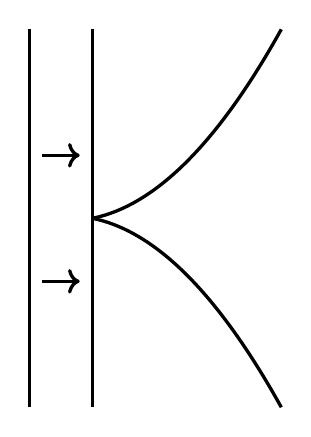
\begin{tikzpicture}[line width=1.2pt, scale=0.8] % 设置全局线条粗细

    % 1. 绘制左侧两条垂直的平行线（代表障碍物或狭缝）
    \draw (0, -3) -- (0, 3);
    \draw (1, -3) -- (1, 3);

    % 2. 绘制两个向右的入射箭头
    \draw[->] (0.2, 1) -- (0.8, 1);
    \draw[->] (0.2, -1) -- (0.8, -1);

    % 3. 绘制右侧向上和向下扩散的曲线（代表衍射波）
    % 使用贝塞尔曲线 (.. controls ..) 模拟平滑扩散的形状
    \draw (1, 0) .. controls (2, 0.2) and (3, 1.2) .. (4, 3);
    \draw (1, 0) .. controls (2, -0.2) and (3, -1.2) .. (4, -3);

\end{tikzpicture}
\end{center}
\end{aside}

\subsection*{射影平面曲线}

$k$ 上的射影平面是
\[
\mathbb{P}^2(k) = \{(x,y,z)\in k^3 \mid (x,y,z)\neq(0,0,0)\}/{\sim},
\]
其中 $(x,y,z)\sim(x',y',z')$ 当且仅当存在 $c\neq 0\in k$ 使 $(x',y',z') = (cx,cy,cz)$. 记 $(x:y:z)$ 为 $(x,y,z)$ 的等价类——冒号意在提示只有比值有意义. 设 $P\in\mathbb{P}^2(k)$, 表示 $P$ 的三元组 $(x,y,z)$ 落在 $k^3$ 中过原点的一条直线 $L(P)$ 上, 且 $P\mapsto L(P)$ 是 $\mathbb{P}^2(k)$ 到所有此类直线集合的双射. 射影 $n$-空间 $\mathbb{P}^n(k)$ 可类似定义.

设 $U_2(k) = \{(x:y:z) \mid z\neq 0\}$, $L_\infty(k) = \{(x:y:z) \mid z = 0\}$. 则
\[
(x,y)\mapsto(x:y:1)\colon\mathbb{A}^2(k)\to U_2(k), \qquad
(x,y)\mapsto(x:y:0)\colon\mathbb{P}^1(k)\to L_\infty(k)
\]
都是双射. 且 $\mathbb{P}^2(k)$ 是 ``仿射平面'' $U_2$ 与 ``无穷远直线'' $L_\infty$ 的无交并:
\[
\mathbb{P}^2(k) = U_2(k)\sqcup L_\infty(k).
\]
直线 $aX + bY + cZ = 0$ ($a,b$ 不全为零) 与 $L_\infty$ 交于点 $(-b:a:0)$, 它只依赖仿射直线 $aX + bY + c = 0$ 的斜率. 可以把 $\mathbb{P}^2$ 想象为仿射平面 $U_2$ 对每一族平行线恰好添上一个点.

一个非常数的齐次多项式 $F\in k[X,Y,Z]$, 假定其在 $k^{\mathrm{al}}$ 中无重复因子, 定义了 $k$ 上的一条射影平面曲线 (projective plane curve)\index{sheyingpingmianquxian@射影平面曲线(projective plane curve)} $C_F$, 它在任一包含 $k$ 的域 $K$ 中的点集为 $F$ 在 $\mathbb{P}^2(K)$ 中的零点:
\[
C_F(K) = \{(x:y:z)\in\mathbb{P}^2(K) \mid F(x,y,z) = 0\}.
\]
注意, 因 $F$ 齐次,
\[
F(cx,cy,cz) = c^{\deg F}F(x,y,z), \qquad c\in k^{\times},
\]
故虽然谈论 $F$ 在 $\mathbb{P}^2$ 的某点 $P$ 处的值无意义, 但谈论 $F$ 在 $P$ 处是否为零是有意义的. 同样, 我们不区分曲线 $C_F$ 与 $C_{cF}$ ($c\in k^{\times}$). 一条平面射影曲线 (唯一地) 是一些不可约射影平面曲线 (由不可约多项式定义的那些) 的并. $F$ 的次数称为曲线 $C_F$ 的次数 (degree).\index{quxiandecishu@曲线的次数(degree of a curve)}

\begin{example} \label{thm:1.1.15} 
曲线
\[
Y^2Z = X^3 + aXZ^2 + bZ^3
\]
与无穷远直线交于点 $(0:1:0)$, 即与所有竖直线相同的一点. 这在几何上是合理的, 因为当 $x\to\infty$ 时, 实仿射曲线 $Y^2 = X^3 + aX + b$ 的切线的斜率趋于无穷 (见前言 p.~\pageref{chapter:intro} 的图).
\end{example}

设 $U_1(k) = \{(x:y:z) \mid y\neq 0\}$, $U_0(k) = \{(x:y:z) \mid x\neq 0\}$. 则 $U_1$ 与 $U_0$ 也以自然方式成为仿射平面:
\[
(x,z)\longleftrightarrow(x:1:z)\colon\mathbb{A}^2(k)\cong U_1(k), \qquad
(y,z)\longleftrightarrow(1:y:z)\colon\mathbb{A}^2(k)\cong U_0(k).
\]
因 $x,y,z$ 至少有一个非零,
\[
\mathbb{P}^2 = U_0\cup U_1\cup U_2.
\]
射影平面曲线 $C = C_F$ 是三条仿射平面曲线的并:
\[
C = C_0\cup C_1\cup C_2, \qquad C_i = C\cap U_i.
\]
{\emergencystretch=3em 把每个 $U_i$ 以自然方式等同于 $\mathbb{A}^2$ 时, $C_0, C_1, C_2$ 分别等同于由多项式 $F(1,Y,Z)$, $F(X,1,Z)$, $F(X,Y,1)$ 定义的仿射曲线.\par}

\begin{example} \label{thm:1.1.16} 
曲线
\[
C\colon Y^2Z = X^3 + aXZ^2 + bZ^3
\]
由两条仿射曲线覆盖, 即
\[
C_2\colon Y^2 = X^3 + aX + b \qquad \text{与} \qquad C_1\colon Z = X^3 + aXZ^2 + bZ^3.
\]
\end{example}

切线、重数、相交数等概念可通过下述方式搬到射影曲线上: 射影曲线 $C$ 的每个点 $P$ 至少位于某个仿射曲线 $C_i$ 上. 若 $P\in C(k)$ 作为某仿射曲线 $C_i$ 的点是非奇异的, 则在所有包含 $P$ 的 $C_i$ 中都非奇异. 其他概念也有类似的结论.

\begin{exercise} \label{thm:1.1.17} 
设 $P$ 是射影平面曲线 $C = C_F$ 上的点. 证明 $P$ 奇异当且仅当
\[
\Bigl(\frac{\partial F}{\partial X}\Bigr)_P = \Bigl(\frac{\partial F}{\partial Y}\Bigr)_P = \Bigl(\frac{\partial F}{\partial Z}\Bigr)_P = 0.
\]
当 $P$ 非奇异时, 证明射影直线
\[
L\colon \Bigl(\frac{\partial F}{\partial X}\Bigr)_P X + \Bigl(\frac{\partial F}{\partial Y}\Bigr)_P Y + \Bigl(\frac{\partial F}{\partial Z}\Bigr)_P Z = 0
\]
具有性质: 对每个满足 $P\in U_i$ 的 $i$, $L\cap U_i$ 是仿射曲线 $C_i$ 在 $P$ 处的切线.
\end{exercise}

\subsection*{Bezout 定理}\index{Bezout@Bezout 定理(Bezout's theorem)}

\begin{theorem}[Bezout] \label{thm:1.1.18} 
设 $C$ 与 $D$ 为 $k$ 上次数分别为 $m$ 与 $n$ 的射影平面曲线, 且无公共分支. 则 $C$ 与 $D$ 在 $k^{\mathrm{al}}$ 上恰好相交于计入重数的 $mn$ 个点, 即
\[
\sum_{P\in C(k^{\mathrm{al}})\cap D(k^{\mathrm{al}})} I(P, C\cap D) = mn.
\]
\end{theorem}

\begin{proof}
初等证明见 \cite[\S5.3]{fulton1969}.
\end{proof}

设 $C$ 与 $D$ 为 $k$ 上次数分别为 $m$ 与 $n$ 的射影平面曲线. 若 $C(k^{\mathrm{al}})\cap D(k^{\mathrm{al}})$ 中恰有 $mn$ 个点, 则 Bezout 定理与 \ref{thm:1.1.13} 表明这些点在 $C$ 与 $D$ 上都非奇异; 若点多于 $mn$ 个, 则曲线必有公共分支.

\begin{aside} \label{thm:1.1.19} 
在 $\mathbb{C}$ 上, 映射
\[
(F,G) \mapsto \sum_{P\in C_F(\mathbb{C})\cap C_G(\mathbb{C})} I(P, C_F\cap C_G)
\]
关于 $F$ 与 $G$ 的系数 (对 $\mathbb{N}$ 的离散拓扑) 连续. 因此总相交数在齐次多项式的连续族上恒定, 这使得在证明 Bezout 定理时可取 $F = X^m$, $G = Y^n$. 则 $P = (0:0:0)$ 是两条曲线上唯一的公共点, 且
\[
I(P, C_{X^m}\cap C_{Y^n}) = I(X^m, Y^n) = mn,
\]
即证得定理. 类似论证对任意域都成立, 只要先证明总相交数在代数族上恒定 (cf.\ \cite[III, 2.2]{shafarevich1994}).
\end{aside}

\begin{example} \label{thm:1.1.20} 
由 Bezout 定理, 一条 $m$ 次曲线与无穷远直线计入重数地恰好交于 $m$ 个点. 我们钟爱的曲线
\[
C\colon Y^2Z = X^3 + aXZ^2 + bZ^3
\]
与 $L_\infty$ 交于唯一点 $P = (0:1:0)$, 但 (见~\ref{thm:1.1.8})
\[
I(P, L_\infty\cap C) = I(Z, Z - X^3 - aXZ - bZ^3) = I(Z, X^3) = 3.
\]
一般地, 曲线 $C$ 上的非奇异点 $P$ 若其切线与 $C$ 在 $P$ 处的相交重数 $\ge 3$, 则称为拐点 (point of inflection, 或 flex).\index{guaidian@拐点(point of inflection)}\footnote{有时还要求相交重数为奇数.} 若相交重数等于 $3$, 则称拐点为普通的 (ordinary).\index{guaidian@拐点(point of inflection)!putong@普通(ordinary)} 三次曲线上的拐点总是普通的.
\end{example}

\begin{remark} \label{thm:1.1.21} 
由 Bezout 定理, 射影平面曲线的任意两个不可约分支都有公共点 (可能在 $k$ 的某个有限扩张中), 该点由~\ref{thm:1.1.4}b 是奇异的. 因此, 非奇异射影平面曲线几何不可约.
\end{remark}

\subsection*{附录：结式}

设 $f(X) = s_0X^m + s_1X^{m-1} + \cdots + s_m$ 与 $g(X) = t_0X^n + t_1X^{n-1} + \cdots + t_n$ 为系数在 $k$ 中的多项式. $f$ 与 $g$ 的结式 (resultant)\index{jieshi@结式(resultant)} $\operatorname{Res}(f,g)$ 定义为行列式
\[
\begin{vmatrix}
s_0 & s_1 & \cdots & s_m & & \\
& s_0 & \cdots & s_{m-1} & s_m & \\
& & \ddots & & & \\
& & & s_0 & s_1 & \cdots & s_m\\
t_0 & t_1 & \cdots & t_n & & \\
& t_0 & \cdots & t_{n-1} & t_n & \\
& & \ddots & & & \\
& & & t_0 & t_1 & \cdots & t_n
\end{vmatrix}
\]
其中有 $n$ 行 $s_i$ 与 $m$ 行 $t_j$, 故矩阵为 $(m+n)\times(m+n)$; 所有空白处填零. 结式是 $f$ 与 $g$ 的系数的多项式.

\begin{proposition} \label{thm:1.1.22} 
结式 $\operatorname{Res}(f,g) = 0$ 当且仅当
\begin{enumerate}[label=\textup{(\alph*)}]
\item $s_0$ 与 $t_0$ 都为零; 或
\item 两多项式在 $k^{\mathrm{al}}$ 中有公共根.\footnote{校对注：原书把公共根写为在 $k$ 中. 对一般域，这应是在 $k^{\mathrm{al}}$ 中；例如在 $k=\mathbb{R}$ 时，$f=g=X^2+1$ 的结式为零，却没有实根. 下文相应地在代数闭包上作根的分解，并将最大公因子的域扩张不变性陈述为非常数公共因子的存在性不变.}
\end{enumerate}
\end{proposition}

\begin{proof}
若 (a) 成立, 则行列式第一列为零, 故 $\operatorname{Res}(f,g) = 0$. 设 $a$ 为 $f$ 与 $g$ 的公共根, 则存在次数分别为 $m-1$ 与 $n-1$ 的多项式 $f_1, g_1\in k^{\mathrm{al}}[X]$ 使
\[
f(X) = (X-a)f_1(X), \qquad g(X) = (X-a)g_1(X).
\]
由这些等式得
\begin{equation} \label{eq:2}
f(X)g_1(X) - g(X)f_1(X) = 0.
\tag{2}
\end{equation}
把 \eqref{eq:2} 中 $X^{m+n-1},\dots,X,1$ 的系数置零, 我们发现 $f_1$ 与 $g_1$ 的系数是 $m+n$ 个未知数、$m+n$ 个线性方程组的解. 方程组的系数矩阵是矩阵 \eqref{eq:3} 的转置:
\begin{equation} \label{eq:3}
\begin{pmatrix}
s_0 & s_1 & \cdots & s_m & & & & \\
& s_0 & \cdots & s_{m-1} & s_m & & & \\
& & \ddots & & & & & \\
& & & s_0 & s_1 & \cdots & s_m & \\
t_0 & t_1 & \cdots & t_n & & & & \\
& t_0 & \cdots & t_{n-1} & t_n & & & \\
& & \ddots & & & & & \\
& & & t_0 & t_1 & \cdots & t_n
\end{pmatrix}
\tag{3}
\end{equation}
解的存在表明该矩阵行列式为零, 由此推出 $\operatorname{Res}(f,g) = 0$.

反之, 设 $\operatorname{Res}(f,g) = 0$ 但 $s_0$ 与 $t_0$ 均非零. 因上述矩阵行列式为零, 可解线性方程找到满足 \eqref{eq:2} 的多项式 $f_1, g_1$. $f$ 的根 $a$ 必也是 $f_1$ 或 $g$ 的根. 若是前者, 从 \eqref{eq:2} 左边消去 $X-a$, 考虑 $f_1/(X-a)$ 的根. 因 $\deg f_1 < \deg f$, 此论证最终导致 $f$ 的一个不是 $f_1$ 的根的根, 故它必是 $g$ 的根.
\end{proof}

注意, $k[X]$ 中多项式 $f,g$ 在 $k[X]$ 中有非常数公共因子当且仅当它们在 $k^{\mathrm{al}}[X]$ 中有非常数公共因子, 因为 Euclid 算法表明两个多项式的最大公因子在域扩张下不变 (\cite[2.10]{milne-ft}).

\begin{example} \label{thm:1.1.23} 
对 $m$ 次首一多项式 $f(X)$, $\operatorname{Res}(f, f') = (-1)^{m(m-1)/2}\operatorname{disc}(f)$. 设 $c_1,\dots,c_{m+n}$ 为矩阵 \eqref{eq:3} 的列. 则
\[
\begin{pmatrix}X^{n-1}f(X)\\ X^{n-2}f\\ \vdots\\ f(X)\\ X^{m-1}g(X)\\ \vdots\\ g(X)\end{pmatrix}
= X^{m+n-1}c_1 + \cdots + 1\cdot c_{m+n},
\]
\footnote{校对注：矩阵 \eqref{eq:3} 有 $n$ 行 $f$ 的系数与 $m$ 行 $g$ 的系数，因此左侧的幂次分别从 $n-1$ 与 $m-1$ 开始；原书在此处把两者互换. 原书随后还混用了 $c_0$ 与 $c_1$，此处统一采用前面定义的 $c_1,\dots,c_{m+n}$.} 故 $\operatorname{Res}(f,g) \overset{\text{def}}{=} \det(c_1,\dots,c_{m+n}) = \det(c_1,\dots,c_{m+n-1}, c)$, 其中 $c$ 是上式左边的向量. 展开最后一个行列式, 得
\[
\operatorname{Res}(f,g) = a(X)f(X) + b(X)g(X),
\]
其中 $a(X)$ 与 $b(X)$ 分别是次数 $\le n-1$ 与 $\le m-1$ 的多项式. 若 $f(X)$ 与 $g(X)$ 的系数在整环 $R$ (例如 $\mathbb{Z}$ 或 $k[Y]$) 中, 则 $\operatorname{Res}(f,g)\in R$, 且多项式 $a(X)$, $b(X)$ 的系数也在 $R$ 中.
\end{example}

\begin{proposition} \label{thm:1.1.24} 
设 $f(X,Y), g(X,Y)\in k[X,Y]$, 且 $r(X)\in k[X]$ 为把 $f, g$ 视为系数在 $k[X]$ 中、关于 $Y$ 的多项式时的结式.
\begin{enumerate}[label=\textup{(\alph*)}]
\item 存在 $a(X,Y), b(X,Y)\in k[X,Y]$ 使
\[
af + bg = r(X)\in k[X]
\]
且 $\deg_Y(a) < \deg_Y(g)$, $\deg_Y(b) < \deg_Y(f)$.
\item 多项式 $r = 0$ 当且仅当 $f$ 与 $g$ 在 $k[X,Y]$ 中有关于 $Y$ 的次数为正的公共因子.\footnote{校对注：原书未限制公共因子关于 $Y$ 的次数. 例如 $f=X$、$g=X(Y+1)$ 有公共因子 $X$，但关于 $Y$ 的结式为 $X$，不为零. 这里的判据来自 $k(X)[Y]$ 中的公共因子，故须排除仅依赖 $X$ 的因子.}
\end{enumerate}
\end{proposition}

\begin{proof}
\begin{enumerate}[label=\textup{(\alph*)}]
\item 由上面的讨论直接得到.
\item 我们知道 $r = 0$ 当且仅当 $f$ 与 $g$ 在 $k(X)[Y]$ 中有公共因子, 但由 Gauss 引理 (\cite[4.5]{milne-ca}), 这等价于它们在 $k[X,Y]$ 中有关于 $Y$ 的次数为正的公共因子.
\end{enumerate}
\end{proof}

\begin{corollary} \label{thm:1.1.25} 
若多项式 $f$ 与 $g$ 在 $k[X,Y]$ 中无公共因子, 则对任意包含 $k$ 的域 $K$, 它们在 $K[X,Y]$ 中无公共因子.
\end{corollary}

\begin{proof}
因 $f$ 与 $g$ 的结式无论我们在 $k$ 上还是在 $K$ 上工作都相同, 这由命题的 (b) 推出.
\end{proof}

\paragraph{齐次多项式的结式}
齐次多项式
\[
F(X,Y) = s_0X^m + s_1X^{m-1}Y + \cdots + s_mY^m, \qquad
G(X,Y) = t_0X^n + t_1X^{n-1}Y + \cdots + t_nY^n
\]
的结式按非齐次情形定义.

\begin{proposition} \label{thm:1.1.26} 
结式 $\operatorname{Res}(F,G) = 0$ 当且仅当 $F$ 与 $G$ 在 $\mathbb{P}^1(k^{\mathrm{al}})$ 中有非平凡零点.
\end{proposition}

\begin{proof}
$F(X,Y)$ 在 $\mathbb{P}^1(k^{\mathrm{al}})$ 中的非平凡零点形如 (a) $(a:1)$, 其中 $a$ 是 $F(X,1)$ 的根; 或 (b) $(1:0)$, 当 $s_0 = 0$ 时. 由于对 $G(X,Y)$ 有类似结论, 本命题是命题 \ref{thm:1.1.22} 的重述.
\end{proof}

计算机代数程序可以计算结式. 例如, 在 Pari/gp 中输入
\begin{verbatim}
polresultant((x+a)^5,(x+b)^5,x)
\end{verbatim}
给出的答案是 $(b-a)^{25}$, 意思是两多项式有公共根当且仅当 $a = b$, 而这可能以 $25$ 种方式发生.

\begin{aside} \label{thm:1.1.27} 
最后一个命题有几何解释. 取 $k$ 代数闭, 把 $F$ 与 $G$ 的系数视为未定元. 设 $V$ 为 $\mathbb{A}^{m+n+2}\times\mathbb{P}^1$ 中 $F(s_0,\dots,s_m;X,Y)$ 与 $G(t_0,\dots,t_n;X,Y)$ 都为零的子集. 命题说 $V$ 在 $\mathbb{A}^{m+n+2}$ 上的投影是 $\operatorname{Res}(F,G)$ (视为 $s_i, t_i$ 的多项式) 为零的集合. 换言之, 命题告诉我们 Zariski 闭集 $V$ 的投影正是由 $F$ 与 $G$ 的结式定义的 Zariski 闭集.

{\emergencystretch=3em 消去理论 (elimination theory) 更一般地做这件事: 对在 $X_i$ 中齐次的多项式 $P_i(T_1,\dots,T_m;\allowbreak X_0,\dots,X_n)$, 它给出寻找多项式 $R_j(T_1,\dots,T_m)$ 的算法, 使 $P_i(a_1,\dots,a_m;\allowbreak X_0,\dots,X_n)$ 有公共零点当且仅当对所有 $j$ 有 $R_j(a_1,\dots,a_m) = 0$. 例如见 \cite[Chap. 8, \S5]{cox2007}.\par}
\end{aside}

\begin{remarkstar}
平面代数曲线的历史可追溯到 2000 多年前——见 \cite[第一章]{brieskorn1986}. Newton\index{Newton} 对实三次平面曲线作了首次系统研究, 把它们分成 72 类 (但漏掉 6 类).
\end{remarkstar}

\section{平面曲线上的有理点}\label{sec:1.2}

对 $\mathbb{Q}$ 上的射影平面曲线 $C_F$, 两个基本问题是:
\begin{enumerate}[label=\textup{(\alph*)}]
\item $C_F$ 是否有坐标在 $\mathbb{Q}$ 中的点, 即 $F(X,Y,Z)$ 是否在 $\mathbb{Q}$ 中有非平凡零点?
\item 若 (a) 的答案是肯定的, 能否描述点集?
\end{enumerate}
还可问是否存在回答这些问题的算法. 例如, 我们可能知道一条曲线只有有限个点, 却没有算法找到这些点或确定其数目.

本节给出该主题的概述. 为简单起见, 全文假设 $C = C_F$ 几何不可约, 即 $F(X,Y,Z)$ 在 $\mathbb{Q}[X,Y,Z]$ 中不可约且在 $\mathbb{Q}^{\mathrm{al}}$ 上仍不可约.

先作一个全书都很有用的观察. 设 $f(X,Y) = \sum a_{ij}X^iY^j$ 为系数 $a_{ij}$ 在域 $k$ 中的多项式, $K$ 为 $k$ 的 Galois 扩张 (可能无限). 若 $(a,b)\in K\times K$ 是 $f(X,Y)$ 的零点, 则对所有 $\sigma\in\operatorname{Gal}(K/k)$, $(\sigma a,\sigma b)$ 也是零点, 因为
\[
f(\sigma a,\sigma b) = \sum a_{ij}(\sigma a)^i(\sigma b)^j = \sigma\Bigl(\sum a_{ij}a^ib^j\Bigr) = \sigma f(a,b) = 0.
\]
因此 $\operatorname{Gal}(K/k)$ 作用在 $C_f(K)$ 上. 更一般地, 若 $C_1, C_2, \dots$ 是 $k$ 上的仿射平面曲线, 则 $\operatorname{Gal}(K/k)$ 稳定 $K\times K$ 的子集 $C_1(K)\cap C_2(K)\cap\cdots$. 把此结论应用于曲线
\[
f = 0, \qquad \frac{\partial f}{\partial X} = 0, \qquad \frac{\partial f}{\partial Y} = 0,
\]
我们看到 $\operatorname{Gal}(K/\mathbb{Q})$ 稳定 $C_f$ 的奇异点集. 对射影平面曲线有类似结论.

\subsection*{一次曲线}

此时曲线是直线
\[
C\colon aX + bY + cZ = 0, \qquad a,b,c\in\mathbb{Q}, \text{ 不全为零}.
\]
它总有坐标在 $\mathbb{Q}$ 中的点, 且可以参数化这些点——例如若 $c\neq 0$, 则映射
\[
(s:t)\mapsto(s:t:-\tfrac{a}{c}s - \tfrac{b}{c}t)
\]
对所有包含 $\mathbb{Q}$ 的域 $K$ 都是 $\mathbb{P}^1(K)$ 到 $C(K)$ 的双射.

\subsection*{二次曲线}

此时 $F(X,Y,Z)$ 是 3 个变量的二次型\index{ercixing@二次型(quadratic form)}, $C$ 是圆锥曲线 (conic). 注意 $C$ 不能奇异: 过重数 $m\ge 2$ 的点 $P$ 的非切线 $L$ 将与 $C$ 交于第二点 $Q$, 而总相交数
\[
I(P, L\cap C) + I(Q, L\cap C) \overset{\text{\ref{thm:1.1.13}}}{\ge} m + 1
\]
违反 Bezout 定理.

有时容易看出 $C(\mathbb{Q})$ 为空. 例如, $X^2 + Y^2 + Z^2$ 在 $\mathbb{Q}$ 中无非平凡零点, 因为它在 $\mathbb{R}$ 中无非平凡零点. 类似地, $X^2 + Y^2 - 3Z^2$ 无非平凡零点, 因为若有, 则它有零点 $(x,y,z)$ 满足 $x,y,z\in\mathbb{Z}$ 且 $\gcd(x,y,z) = 1$; $\mathbb{Z}/3\mathbb{Z}$ 中只有 $0$ 与 $1$ 是平方, 故
\[
x^2 + y^2 \equiv 0 \pmod{3} \implies x\equiv 0\equiv y \pmod{3};
\]
但此时 $3$ 整除 $z$, 与假设 $\gcd(x,y,z) = 1$ 矛盾.

1785 年, Legendre 表明此类论证可以变成判定 $C_F(\mathbb{Q})$ 是否非空的程序. 他先证明, 经初等变量替换, $F$ 可化为对角形式
\[
F = aX^2 + bY^2 + cZ^2, \qquad a,b,c\in\mathbb{Z}, \ a,b,c \text{ 无平方因子}.
\]
他再证明, 若 $abc\neq 0$ 且 $a,b,c$ 不全同号, 则 $F(X,Y,Z)$ 在 $\mathbb{Q}$ 中有非平凡零点当且仅当 $-bc$, $-ca$, $-ab$ 分别是模 $a$, $b$, $c$ 的平方. 由二次互反律\index{dingli@定理(theorem)!ercihufanlv@二次互反律(quadratic reciprocity law)} (IV\ref{thm:4.8.5}), 这蕴含: 存在以简单方式依赖于 $F$ 系数的整数 $m$, 使 $C_F(\mathbb{Q})\neq\varnothing$ 当且仅当 $F(X,Y,Z)\equiv 0\pmod{m}$ 有与 $m$ 互素的整数解. 见~\ref{thm:1.2.18}.

现在设 $C$ 有坐标在 $\mathbb{Q}$ 中的点 $P_0$. 能否描述所有点? $\mathbb{Q}$ 上的直线计入重数地总是与 $C$ 恰好交于两点 (Bezout 定理). 若两点重合, 则直线与 $C$ 相切. 否则, 点对在 $\operatorname{Gal}(\mathbb{Q}^{\mathrm{al}}/\mathbb{Q})$ 的作用下稳定, 故若其中一点系数在 $\mathbb{Q}$ 中, 则两点都在. $\mathbb{P}^2$ 中过 $P_0$ 的直线构成一个 ``$\mathbb{P}^1$'', 把过 $P_0$ 的直线送到其第二个交点, 是 $\mathbb{P}^1(\mathbb{Q})$ 到 $C(\mathbb{Q})$ 的双射. 例如, 取 $P_0$ 为曲线 $C\colon X^2 + Y^2 = Z^2$ 上的点 $(-1:0:1)$. 过 $P_0$、斜率为 $b/a$ ($a,b\in\mathbb{Q}$) 的直线 $bX - aY + bZ$ 与 $C$ 交于点 $(a^2-b^2 : 2ab : a^2+b^2)$. 这样, 我们得到 $C$ 上坐标在 $\mathbb{Q}$ 中的点的参数化 $(a:b)\mapsto(a^2-b^2:2ab:a^2+b^2)$.

\subsection*{三次曲线}

设 $C\colon F(X,Y,Z) = 0$ 为 $\mathbb{Q}$ 上次数 $3$ 的射影平面曲线. 若 $C$ 奇异, 则 Bezout 定理表明它只有一个奇异点, 且其重数为 $2$. 奇异点 $P_0$ 的坐标在 $\mathbb{Q}$ 的某个有限扩张 $K$ 中, 可取 $K$ 在 $\mathbb{Q}$ 上 Galois, 但 $\operatorname{Gal}(K/\mathbb{Q})$ 稳定 $C(K)$ 中的奇异点集, 故固定 $P_0$, 从而 $P_0\in C(\mathbb{Q})$. 此时过 $P_0$ 的直线与曲线恰好交于另一个点 (可能与 $P_0$ 重合), 故再次得到 $C$ 上坐标在 $\mathbb{Q}$ 中的点的参数化.

非奇异三次曲线将是本书其余部分的主题. 我们将看到 Legendre 的论证对非奇异三次曲线失败. 例如,
\[
3X^3 + 4Y^3 + 5Z^3
\]
有非平凡的实零点, 且对每个整数 $m$ 有非平凡模 $m$ 零点, 但它在 $\mathbb{Q}$ 中没有非平凡零点.

设 $C$ 为 $\mathbb{Q}$ 上的非奇异三次曲线. 由 Bezout 定理, 直线计入重数地与曲线交于三点. 若其中两点系数在 $\mathbb{Q}$ 中, 则第三点也系数在 $\mathbb{Q}$ 中.\footnote{把 $Y = aX + b$ 代入定义仿射三次曲线的多项式, 得到 $X$ 的系数在 $\mathbb{Q}$ 中的三次多项式, 其两个根在 $\mathbb{Q}$ 中; 于是第三个根也在 $\mathbb{Q}$ 中.} 因此, $C(\mathbb{Q})$ 中两点的弦与曲线交于 $C(\mathbb{Q})$ 中的第三点, 且 $C(\mathbb{Q})$ 中某点的切线与曲线交于 $C(\mathbb{Q})$ 中的另一点.

在一篇著名的论文 (1922 年发表) 中, Mordell\index{Mordell} 证明了以下定理.

\begin{theorem}[有限基定理] \label{thm:1.2.1}\index{dingli@定理(theorem)!youxianji@有限基定理(finite basis theorem)} 
设 $C$ 为 $\mathbb{Q}$ 上的非奇异三次曲线. 则存在 $C(\mathbb{Q})$ 中的有限点集, 使 $C(\mathbb{Q})$ 中其他每个点都能由这些点经反复的弦与切线构造而得到.
\end{theorem}

事实上, $C(\mathbb{Q})$ 若非空, 则有自然的交换群结构 (见下节), 而有限基定理说 $C(\mathbb{Q})$ 有限生成. 迄今仍无被证明的算法可求该群的秩.

\begin{remark} \label{thm:1.2.2} 
对 $\mathbb{Q}$ 上的奇异三次曲线 $C$, 非奇异点仍构成群, 可能同构于 $(\mathbb{Q},+)$ 或 $(\mathbb{Q}^{\times},\times)$ (见 II, \S\ref{sec:2.3}), 两者都不有限生成——$(\mathbb{Q},+)$ 的任何有限生成子群中元素有公共分母, 而 $(\mathbb{Q}^{\times},\times)$ 的有限生成子群只能含有限多个素数. 因此, 有限基定理对奇异三次曲线失败.
\end{remark}

\subsection*{亏格 $> 1$ 的曲线}

$\mathbb{Q}$ 上非奇异射影曲线 $C$ 的亏格 (genus)\index{kuige@亏格(genus)} 是 Riemann 曲面 $C(\mathbb{C})$ 的亏格. 更一般地, $\mathbb{Q}$ 上任意曲线的亏格是其函数域\index{hanshuyu@函数域(function field)}所对应的非奇异射影曲线的亏格 (\cite[\S7.5, Cor.\ to Theorem 3]{fulton1969}). Mordell 在 1922 年的论文中猜想, \cite{faltings1983} 证明了: 亏格 $> 1$ 的每条曲线都只有有限多个坐标在 $\mathbb{Q}$ 中的点. 这适用于次数至少为 $4$ 的每条非奇异射影平面曲线, 也适用于次数相对其奇点重数足够大的每条奇异射影平面曲线 (见本章后面的 \ref{thm:1.6.5}).

\begin{remark} \label{thm:1.2.3} 
设 $P\in\mathbb{P}^2(\mathbb{Q})$. 选取 $P$ 的代表元 $(a:b:c)$, 其中 $a,b,c$ 为无公因子的整数, 定义 $P$ 的高度 (height) $H(P) = \max(|a|,|b|,|c|)$. 对任意 $B > 0$, 只有有限多个 $P$ 满足 $H(P) < B$.

对亏格 $> 1$ 的曲线 $C$, 存在 $C(\mathbb{Q})$ 中点数的有效界, 但就定义 $C$ 的多项式而言, 对 $P\in C(\mathbb{Q})$ 的高度没有已知的有效界. 若有这样的界, 则通过有限搜索即可找到 $C(\mathbb{Q})$ 中的点. 见 \cite[F.4.2]{hindry2000} 对该问题的讨论.
\end{remark}

\begin{aside} \label{thm:1.2.4} 
对 Mordell 猜想有启发式解释. 设 $C$ 为 $\mathbb{Q}$ 上亏格 $g\ge 1$ 的曲线. 若 $C(\mathbb{Q})$ 非空, 则 $C$ 嵌入其 Jacobi 簇 $J$, 后者是维数 $g$、带群结构的射影簇, 即 阿贝尔簇. Weil\index{Weil} 推广的有限基定理说 $J(\mathbb{Q})$ 有限生成. 因此在 $g$ 维集合 $J(\mathbb{C})$ 中, 有可数集 $J(\mathbb{Q})$ 和 (看起来无关的) 一维集 $C(\mathbb{C})$. 若 $g > 1$, 第二个集合含第一个集合中多于有限多个元素将是非同寻常的巧合.
\end{aside}

为继续讨论, 我们需要 $p$-进数域.

\subsection*{$p$-进数简介}

设 $p$ 为素数. 非零有理数 $a$ 可唯一表示为 $a = p^r\frac{m}{n}$, 其中 $m, n, r$ 为整数且 $m, n$ 不被 $p$ 整除. 令 $|a|_p = \frac{1}{p^r}$, 且 $|0|_p = 0$. 称 $|a|_p$ 为 $a$ 的 $p$-进赋值. 它有如下性质:
\begin{enumerate}[label=\textup{(\alph*)}]
\item $|a|_p = 0$ 当且仅当 $a = 0$;
\item $|ab|_p = |a|_p|b|_p$;
\item $|a+b|_p\le\max\{|a|_p,|b|_p\}$ ($\le |a|_p + |b|_p$).
\end{enumerate}
这些论断蕴含
\[
d_p(a,b) \overset{\text{def}}{=} |a-b|_p
\]
是 $\mathbb{Q}$ 上的平移不变度量, 称为 $p$-进度量. 注意对此度量而言有理数 $a, b$ 接近意味着它们的差被 $p$ 的高次幂整除. $p$-进数域 $\mathbb{Q}_p$ 是 $\mathbb{Q}$ 关于此度量的完备化. 下面解释这是什么意思.

有理数序列 $a_1, a_2, a_3, \dots$ 关于 $p$-进度量是 Cauchy 序列\index{Cauchy-xulie@Cauchy 序列(Cauchy sequence)}, 若对每个实数 $\varepsilon > 0$, 存在自然数 $N(\varepsilon)$ 使当 $m, n > N(\varepsilon)$ 时有 $|a_m - a_n|_p < \varepsilon$. 序列 $a_1, a_2, a_3, \dots$ 收敛到 $a\in\mathbb{Q}$, 若对每个实数 $\varepsilon > 0$, 存在自然数 $N(\varepsilon)$ 使当 $n > N(\varepsilon)$ 时有 $|a_n - a|_p < \varepsilon$.

设 $R$ 为 $\mathbb{Q}$ 中关于 $p$-进度量的一切 Cauchy 序列的集合. 用显然的运算它成为环. $R$ 的元素称为零的 (null), 若它收敛到 $0$. 零序列的集合是 $R$ 的理想 $I$, 而 $\mathbb{Q}_p$ 定义为商环 $R/I$. 它是域.

若 $\alpha = (a_n)_{n\ge 1}$ 是 $\mathbb{Q}$ 中的 Cauchy 序列, 则由性质 (c), 序列 $|a_n|_p$ 对大 $n$ 变成常数, 设此常数值为 $|\alpha|_p$. 映射 $\alpha\mapsto|\alpha|_p\colon R\to\mathbb{Q}$ 穿过 $\mathbb{Q}_p$ 且具有上面列出的性质 (a), (b), (c). 因此 $\mathbb{Q}$ 上的 $p$-进度量延拓到 $\mathbb{Q}_p$.

\begin{theorem} \label{thm:1.2.5} 
\begin{enumerate}[label=\textup{(\alph*)}]
\item 域 $\mathbb{Q}_p$ 完备, 即 $\mathbb{Q}_p$ 中每个 Cauchy 序列收敛到 $\mathbb{Q}_p$ 中的极限.
\item 把 $a\in\mathbb{Q}$ 送到常数 Cauchy 序列 $a,a,a,\dots$ 的等价类的映射, 是像稠密的单射同态 $\mathbb{Q}\hookrightarrow\mathbb{Q}_p$.
\end{enumerate}
\end{theorem}

\begin{proof}
练习.
\end{proof}

$p$-进整数环 $\mathbb{Z}_p$ 定义为 $\mathbb{Z}$ 在 $\mathbb{Q}_p$ 中的闭包. 这正是满足 $|\alpha|_p\le 1$ 的 $\alpha\in\mathbb{Q}_p$ 的集合. 每个 $p$-进整数 $a$ 可由唯一的级数表示:
\[
a_0 + a_1p + \cdots + a_ip^i + \cdots, \qquad 0\le a_i\le p-1,
\]
即存在唯一的整数序列 $a_0, a_1, \dots$ ($0\le a_i\le p-1$) 使上述级数的部分和构成表示 $a$ 的 Cauchy 序列. $a_i$ (若存在) 满足同余式
\[
a_0\equiv a \pmod{p\mathbb{Z}}, \quad \dots, \quad a_i \equiv \frac{a - (a_0 + \cdots + a_{i-1}p^{i-1})}{p^i} \pmod{p\mathbb{Z}}, \ \dots
\]
这证明了唯一性, 而这些同余式可用于归纳地定义 $a_i$: 利用 $\mathbb{Z}$ 在 $\mathbb{Z}_p$ 中稠密, 可得
\[
\mathbb{Z}/p^m\mathbb{Z} \cong \mathbb{Z}_p/p^m\mathbb{Z}_p, \qquad \text{所有 } m\ge 1.
\]
取极限, 得同构
\[
\varprojlim \mathbb{Z}/p^m\mathbb{Z} \cong \varprojlim \mathbb{Z}_p/p^m\mathbb{Z}_p \cong \mathbb{Z}_p.
\]

\begin{remark} \label{thm:1.2.6} 
\begin{enumerate}[label=\textup{(\alph*)}]
\item 上面的构造若把 $|\cdot|_p$ 换成通常的绝对值, 得到的是 $\mathbb{R}$ 而非 $\mathbb{Q}_p$.
\item 正如实数可用小数表示, $p$-进数可表示为如下形式的无穷级数:
\[
a_{-n}p^{-n} + \cdots + a_0 + a_1p + \cdots + a_mp^m + \cdots, \qquad 0\le a_i\le p-1.
\]
这可通过 $\mathbb{Q}_p^{\times} = p^{\mathbb{Z}}\cdot\mathbb{Z}_p^{\times}$ (直积) 证明.
\end{enumerate}
$p$-进整数环 $\mathbb{Z}_p$ 紧致, 且它在 $\mathbb{Q}_p$ 中开. 因此 $\mathbb{Q}_p$ 局部紧致. $p$-进数与当前讨论的相关性由下一个论断解释.

设 $f(X_0,\dots,X_n)\in\mathbb{Z}[X_0,\dots,X_n]$ 为齐次型. 假设对每个自然数 $N$, 存在整数 $a_0^{(N)},\dots,a_n^{(N)}$, 不全被 $p$ 整除, 使
\begin{equation} \label{eq:4}
f(a_0^{(N)},\dots,a_n^{(N)}) \equiv 0 \pmod{p^N}.
\tag{4}
\end{equation}
因 $\mathbb{Z}_p^{n+1}$ 紧致, 集合 $\{(a_0^{(N)},\dots,a_n^{(N)}) \mid N\in\mathbb{N}\}$ 在 $\mathbb{Z}_p^{n+1}$ 中有极限点 $(\alpha_0,\dots,\alpha_n)$, 且容易看出
\begin{equation} \label{eq:5}
f(\alpha_0,\dots,\alpha_n) = 0.
\tag{5}
\end{equation}
反之, 设 $(\alpha_0,\dots,\alpha_n)\in\mathbb{Q}_p^{n+1}$ 满足 \eqref{eq:5} 且不全为零. 缩放后可设 $\max_i|\alpha_i|_p = 1$. 对每个 $N\in\mathbb{N}$, 选取整数 $a_0^{(N)},\dots,a_n^{(N)}$ 使对所有 $j$ 有 $|a_j^{(N)} - \alpha_j|\le p^{-N}$. 则 $(a_0^{(N)},\dots,a_n^{(N)})$ 满足 \eqref{eq:4}.
\end{remark}

\begin{notation} \label{thm:1.2.7}\index{padic@p-进赋值(p-adic valuation)}
对 $a\in\mathbb{Q}^{\times}$, 若 $a = p^r\frac{m}{n}$ 且 $m, n$ 不被 $p$ 整除, 则令 $\ord\nolimits_p(a) = r$; 且令 $\ord\nolimits_p(0) = \infty$. 关于 $\infty$ 采用显然的约定, 我们有
\begin{enumerate}[label=\textup{(\alph*)}]
\item $\ord\nolimits_p(a) = \infty$ 当且仅当 $a = 0$;
\item $\ord\nolimits_p(ab) = \ord\nolimits_p(a) + \ord\nolimits_p(b)$;
\item $\ord\nolimits_p(a+b)\ge\min\{\ord\nolimits_p(a),\ord\nolimits_p(b)\}$, 且除非 $\ord\nolimits_p(a) = \ord\nolimits_p(b)$ 否则严格大于.
\end{enumerate}
特别地, $\ord\nolimits_p$ 是同态 $\mathbb{Q}^{\times}\to\mathbb{Z}$. 该同态由连续性延拓到 $\mathbb{Q}_p^{\times}$.
\end{notation}

\begin{remarkstar}
关于 $p$-进数更从容的讲解, 例如见 \cite{koblitz1977} 的第一章. 据 Ostrowski 定理\index{Ostrowski@Ostrowski 定理(Ostrowski's theorem)}, $\mathbb{R}$ 与各 $p$-进域 $\mathbb{Q}_p$ 是 $\mathbb{Q}$ 关于非平凡赋值仅有的完备化.
\end{remarkstar}

\subsection*{二次曲线与三次曲线续}

显然, 曲线有坐标在 $\mathbb{Q}$ 中的点的必要条件是它在 $\mathbb{R}$ 与所有 $\mathbb{Q}_p$ 中有坐标在其中的点. 事实上, 我们上面已观察到 $X^2 + Y^2 + Z^2$ 在 $\mathbb{Q}$ 中无非平凡零点, 因为它在 $\mathbb{R}$ 中无非平凡实零点; 而我们对 $X^2 + Y^2 - 3Z^2$ 的论证表明它在 $3$-进数域 $\mathbb{Q}_3$ 中无非平凡零点. Legendre 定理的现代解释是: 对二次曲线, 该条件也是充分的.

\begin{theorem}[Legendre] \label{thm:1.2.8} 
系数在 $\mathbb{Q}$ 中的二次型 $F(X,Y,Z)$ 在 $\mathbb{Q}$ 中有非平凡零点, 当且仅当它在 $\mathbb{R}$ 与所有 $\mathbb{Q}_p$ 中有非平凡零点.
\end{theorem}

\begin{proof}
见 \cite[Chapter 3]{cassels1991} 或 \cite[Chapter IV]{serre1973}.
\end{proof}

见下面 \ref{thm:1.2.18} 关于此陈述与 Legendre 原始陈述的关系.

\begin{aside} \label{thm:1.2.9} 
定理 \ref{thm:1.2.8} 对任意变量个数的二次型成立 (Hasse\index{Hasse}--Minkowski 定理). 证明的很好的讲解见 \cite[Chap.~IV]{serre1973}. 关键情形是 $3$ 个与 $4$ 个变量 ($2$ 个变量容易, 对 $\ge 5$ 个变量用关于 $n$ 的归纳), 证明所需的关键结果是二次互反律 (IV\ref{thm:4.8.5}).

若对某类多项式 (或代数簇\index{daishucu@代数簇(algebraic variety)}) 已知: 它在 $\mathbb{Q}$ 中有零点当且仅当它在 $\mathbb{R}$ 与所有 $\mathbb{Q}_p$ 中有零点, 则称该类满足 Hasse 原理, 或局部--整体原理 (local-global principle).\index{Hasse@Hasse 原理(Hasse principle)}\index{jubuzhengtiliyuanli@局部--整体原理(local-global principle)}
\end{aside}

\subsection*{Hensel 引理}

\begin{lemma} \label{thm:1.2.10} 
设 $f(X_1,\dots,X_n)\in\mathbb{Z}[X_1,\dots,X_n]$, $a\in\mathbb{Z}^n$ 满足: 对某个 $m\ge 0$,
\[
f(a) \equiv 0 \pmod{p^{2m+1}},
\]
但对某个 $i$,
\[
\Bigl(\frac{\partial f}{\partial X_i}\Bigr)(a) \not\equiv 0 \pmod{p^{m+1}}.
\]
则存在 $b\in\mathbb{Z}^n$ 使
\[
b\equiv a \pmod{p^{m+1}} \qquad \text{且} \qquad f(b)\equiv 0 \pmod{p^{2m+2}}.
\]
\end{lemma}

\begin{proof}
考虑泰勒展开
\[
f(X_1,\dots,X_n) = f(a_1,\dots,a_n) + \sum_{i=1}^n\Bigl(\frac{\partial f}{\partial X_i}\Bigr)_a(X_i - a_i) + \text{次数 }\ge 2 \text{ 的项}.
\]
令 $b_i = a_i + h_ip^{m+1}$, $h_i\in\mathbb{Z}$. 则
\[
f(b_1,\dots,b_n) = f(a_1,\dots,a_n) + \sum_{i=1}^n\Bigl(\frac{\partial f}{\partial X_i}\Bigr)_a h_ip^{m+1} + \text{被 } p^{2m+2} \text{ 整除的项}.
\]
我们必须选取 $h_i$ 使
\[
f(a_1,\dots,a_n) + \sum_{i=1}^n\Bigl(\frac{\partial f}{\partial X_i}\Bigr)_a h_ip^{m+1}
\]
被 $p^{2m+2}$ 整除. 由假设, 存在 $k\le m$ 使 $p^k$ 整除所有的 $\bigl(\frac{\partial f}{\partial X_i}\bigr)_a$, 但 $p^{k+1}$ 不整除它们的全部. 任何满足下式的 $h_i$ 都可以:
\[
\frac{f(a_1,\dots,a_n)}{p^{k+m+1}} + \sum_{i=1}^n\frac{\bigl(\frac{\partial f}{\partial X_i}\bigr)_a}{p^k}h_i \equiv 0 \pmod{p}.
\]
\end{proof}

\begin{remark} \label{thm:1.2.11} 
若引理中 $a$ 满足条件 $f(a)\equiv 0\pmod{p^{2m+r}}$ 对某个 $r\ge 1$, 则证明中的构造给出 $b$ 使 $b\equiv a\pmod{p^{m+r}}$ 且 $f(b)\equiv 0\pmod{p^{2m+r+1}}$.
\end{remark}

\begin{theorem}[Hensel 引理] \label{thm:1.2.12}\index{yinli@引理(lemma)!Hensel@Hensel(Hensel)} 
在引理的假设下, 存在 $b\in\mathbb{Z}_p^n$ 使 $f(b) = 0$ 且 $b\equiv a\pmod{p^{m+1}}$.
\end{theorem}

\begin{proof}
{\emergencystretch=3em 对引理应用, 得到 $a_{2m+2}\in\mathbb{Z}^n$ 使 $a_{2m+2}\equiv a\pmod{p^{m+1}}$ 且 $f(a_{2m+2})\equiv 0\pmod{p^{2m+2}}$. 第一个同余蕴含\par}
\[
\Bigl(\frac{\partial f}{\partial X_i}\Bigr)(a_{2m+2}) \equiv \Bigl(\frac{\partial f}{\partial X_i}\Bigr)(a) \pmod{p^{m+1}},
\]
{\emergencystretch=3em 故对某个 $i$, $\bigl(\frac{\partial f}{\partial X_i}\bigr)(a_{2m+2})\not\equiv 0\pmod{p^{m+1}}$. 对引理后的注记应用, 得到 $a_{2m+3}\in\mathbb{Z}^n$ 使 $a_{2m+3}\equiv a_{2m+2}\pmod{p^{m+2}}$ 且 $f(a_{2m+3})\equiv 0\pmod{p^{2m+3}}$. 如此继续, 得到 $n$-元组 Cauchy 序列 $a, a_{2m+2},$
$a_{2m+3}, \dots$. 设 $b$ 为它在 $\mathbb{Z}_p^n$ 中的极限. 映射 $f\colon\mathbb{Z}^n\to\mathbb{Z}$ 关于 $p$-进拓扑连续, 故\par}
\[
f(b) = f\Bigl(\lim_r a_{2m+r}\Bigr) = \lim_r f(a_{2m+r}) = 0.
\]
\end{proof}

\begin{example} \label{thm:1.2.13} 
设 $f(X)\in\mathbb{Z}[X]$, $\bar{f}(X)\in\mathbb{F}_p[X]$ 为它的模 $p$ 约化. 设 $a\in\mathbb{Z}$ 使 $\bar{a}\in\mathbb{F}_p$ 是 $\bar{f}(X)$ 的单根. 则 $\frac{d\bar{f}}{dX}(\bar{a})\neq 0$, 故定理表明 $\bar{a}$ 提升为 $f(X)$ 在 $\mathbb{Z}_p$ 中的根.
\end{example}

\begin{example} \label{thm:1.2.14} 
设 $F(X,Y,Z)$ 为 $\mathbb{Z}[X,Y,Z]$ 中的齐次多项式, $(a:b:c)\in\mathbb{P}^2(\mathbb{F}_p)$ 为曲线 $C_F$ 在 $\mathbb{F}_p$ 上的非奇异点. 则如上例, $(a:b:c)$ 提升为曲线 $C_F$ 上坐标在 $\mathbb{Z}_p$ 中的点.
\end{example}

\begin{example} \label{thm:1.2.15} 
设 $f(X,Y,Z)$ 为系数在 $\mathbb{Z}$ 中、判别式 $D\neq 0$ 的二次型. 若 $p\nmid D$, 则 $\bar{f}(X,Y,Z)$ 是 $\mathbb{F}_p$ 上判别式非零的二次型, 已知这样的型在 $\mathbb{F}_p$ 中有非平凡零点 (\cite[I, \S2]{serre1973}). 因此 $f(X,Y,Z)$ 在 $\mathbb{Q}_p$ 中有非平凡零点. 若 $p\mid D$, 则 Hensel 引理表明 $f(X,Y,Z)$ 若有``近似''零点, 则在 $\mathbb{Q}_p$ 中有非平凡零点.
\end{example}

\begin{exercise} \label{thm:1.2.16} 
设
\[
F(X,Y,Z) = 5X^2 + 3Y^2 + 8Z^2 + 6(YZ + ZX + XY).
\]
求 $(a,b,c)\in\mathbb{Z}^3$, 不全被 $13$ 整除, 使
\[
F(a,b,c)\equiv 0 \pmod{13^2}.
\]
\end{exercise}

\begin{exercise} \label{thm:1.2.17} 
考虑仿射平面曲线 $C\colon Y^2 = X^3 + p$. 证明约化曲线 $\bar{C}$ 在 $\mathbb{F}_p$ 上的点 $(0,0)$ 不能提升为 $C$ 上坐标在 $\mathbb{Z}_p^2$ 中的点. 这为什么不违反 Hensel 引理?
\end{exercise}

\begin{aside} \label{thm:1.2.18} 
设 $f(X,Y,Z)$ 为系数在 $\mathbb{Q}$ 中、判别式非零的二次型. 经初等变量替换, 可设 $f = aX^2 + bY^2 + cZ^2$ 且 $a,b,c$ 为无平方因子的整数. 若 $a, b, c$ 有公共素因子 $p$, 则用 $p^{-1}f$ 替换 $f$. 若两个系数 (譬如 $a$ 与 $b$) 有公共素因子 $p$, 则把 $Z$ 换成 $pZ$ 再除以 $p$. 因此, 在研究 $f = 0$ 的解时, 可设
\[
f(X,Y,Z) = aX^2 + bY^2 + cZ^2, \qquad a,b,c\in\mathbb{Z}, \ abc \text{ 无平方因子}.
\]
回忆 Legendre 证明 $f = 0$ 有非零解当且仅当
\begin{enumerate}[label=\textup{(\alph*)}]
\item $a,b,c$ 不全同号, 且
\item $-bc$, $-ca$, $-ab$ 分别是模 $a$, $b$, $c$ 的平方.
\end{enumerate}
我们证明条件 (a), (b) 的必要性. 设 $f = 0$ 有非零解 $(x,y,z)\in\mathbb{Q}^3$. 则当然 (a) 成立. 可设 $x,y,z\in\mathbb{Z}$ 且两两互素. 若 $x$ 与 $c$ 有公共素因子 $p$, 则 $p$ 整除 $y$, 与假设矛盾. 因此 $x$ 模 $c$ 可逆, 由 $ax^2 + by^2 + cz^2 = 0$ 推出 $-ab = (byx^{-1})^2$ 模 $c$. 类似地, $-bc$ 与 $-ca$ 分别是模 $a$ 与 $b$ 的平方.

我们证明 Legendre 原始定理蕴含定理 \ref{thm:1.2.9}: 若 $f$ 在 $\mathbb{R}$ 与对所有整除 $abc$ 的 $p$ 在 $\mathbb{Q}_p$ 中有非平凡零点, 则 Legendre 条件 (a), (b) 成立. 当然 (a) 成立. 设 $c = \prod_i p_i^{r_i}$. 因 $f$ 在 $\mathbb{Q}_{p_i}$ 中有非平凡零点, 上段论证表明 $-ab$ 是 $\mathbb{Z}_{p_i}/c\mathbb{Z}_{p_i} = \mathbb{Z}_{p_i}/p_i^{r_i}\mathbb{Z}_{p_i}$ 中的平方. 由于
\[
\mathbb{Z}/c\mathbb{Z} \cong \prod_i \mathbb{Z}/p_i^{r_i}\mathbb{Z} \qquad \text{(中国剩余定理)} \cong \prod_i \mathbb{Z}_{p_i}/p_i^{r_i}\mathbb{Z}_{p_i},
\]
推出 $-ab$ 是 $\mathbb{Z}/c\mathbb{Z}$ 中的平方. 类似地, $-bc$ 与 $-ca$ 分别是模 $a$ 与 $b$ 的平方.

定理 \ref{thm:1.2.9} 蕴含 Legendre 原始定理的证明同样初等, 只稍微长一点 (\cite{liu2019}).
\end{aside}

\begin{remarkstar}
用于构造新有理点的切线法可追溯到丢番图 (Diophantus\index{Diophantus}, 约公元 250 年), 且``深受费马喜爱''; 弦法为 Newton 所知. Hilbert\index{Hilbert} 与 Hurwitz\index{Hurwitz} 在 1890 年证明: 亏格零的曲线若有一个有理点, 则有无限多个, 全部由参数的整数值给出. 1901 年, Poincar\'e 发表了一篇关于曲线上有理点的长文, 试图把该主题从仅仅是关于单个方程的临时结果的集合中拯救出来. 虽然他通常被归功于猜想了有限基定理, 但他实际上是简单地假设了它. Beppo Levi 是第一个明确询问有限基定理是否成立的人. 在他非凡的 1922 年论文中, Mordell 证明了有限基定理, 并以相当随意的态度猜想 $\mathbb{Q}$ 上所有亏格 $> 1$ 的曲线都只有有限多个有理点 (Mordell 猜想). 两者都极其重要: 前者是丢番图几何的第一个一般定理, 后者是该主题最重要的未解决猜想之一, 直到 1983 年被 Faltings\index{Faltings} 证明.

关于这些主题的更多历史, 见 \cite{cassels1986}, \cite{schappacher1990} 与 \cite{schappacher1996}, 上述注释大部分取材于此.
\end{remarkstar}

\section{三次平面曲线上的群结构}\label{sec:1.3}

设 $C$ 为域 $k$ (为简单起见取为完美域) 上次数 $3$ 的非奇异射影平面曲线. 假设 $C(k)$ 非空, 选取点 $O\in C(k)$. 本节给出 $C(k)$ 上以 $O$ 为零元的群结构的几何构造.

由 Bezout 定理, 直线计入重数地与曲线交于三点. 给定 $P,Q\in C(k)$ (两者都不在对方处的切线上), 记 $PQ$ 为过 $P$ 与 $Q$ 的直线与 $C$ 的第三个交点. 给定 $P\in C(k)$, 记 $PP$ 为 $C$ 在 $P$ 处的切线与 $C$ 的第二个交点. 点 $PQ$ 与 $PP$ 的坐标在 $k$ 中.\footnote{当然, 存在 $k$ 的有限 Galois 扩张 $K$ 使 $PQ\in C(K)$, 但此时 $\operatorname{Gal}(K/k)$ 作用在集合 $\{P,Q,PQ\}$ 上, 故固定 $PQ$. 类似地 $PP\in C(k)$.} 注意 $PP = P$ 当且仅当 $P$ 是拐点.

对一对点 $P,Q\in C(k)$, 定义
\[
P + Q = O(PQ),
\]
即先画过 $P$ 与 $Q$ 的直线得到 $PQ$, 再画过 $O$ 与 $PQ$ 的直线得到 $P+Q$, 如下图所示:

\begin{center}
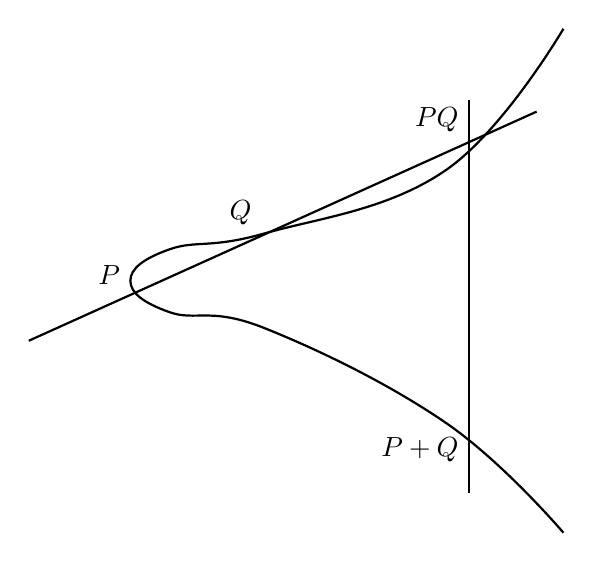
\begin{tikzpicture}[scale=1, thick]
    % 绘制椭圆曲线（上半支与下半支对称）
    \draw[thick] plot[smooth, tension=0.7] coordinates {
        (5, 3.2) (3.5, 1.4) (1.2, 0.6) (0, 0.4) (-0.5, 0) (0, -0.4) (1.2, -0.6) (3.
5, -1.8) (5, -3.2)
    };

    % 定义点坐标
    \coordinate (P) at (-0.5, -0.18);
    \coordinate (Q) at (0.9, 0.58);
    \coordinate (PQ) at (3.8, 1.76);
    \coordinate (PplusQ) at (3.8, -2.15);

    % 绘制割线（穿过 P, Q, PQ）
    \draw[thick] ($(P)!-0.3!(PQ)$) -- ($(P)!1.2!(PQ)$);

    % 绘制垂直线（穿过 PQ 和 P+Q）
    \draw[thick] (3.8, 2.3) -- (3.8, -2.7);

    % 标注各个点
    \node[above left] at (P) {$P$};
    \node[above] at (Q) {$Q$};
    \node[above left] at (PQ) {$PQ$};
    \node[left] at (PplusQ) {$P+Q$};
\end{tikzpicture}
\end{center}

\begin{theorem} \label{thm:1.3.1} 
上述构造使 $C(k)$ 成为交换群.
\end{theorem}

首先注意定义不依赖 $P,Q$ 的次序, 故
\[
P + Q = Q + P.
\]
其次注意
\[
O + P \overset{\text{def}}{=} O(OP) = P,
\]
故 $O$ 是中性元.

给定 $P\in C(k)$, 令 $P' = P(OO)$. 则 $PP' = OO$, 且 $O(PP') = O(OO) = O$, 即 $P + P' = O$.

\begin{center}
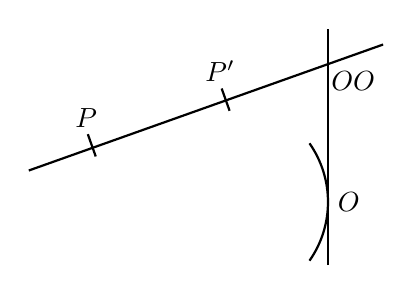
\begin{tikzpicture}[>=stealth, scale=1]
    % 1. 定义直线
    % 倾斜直线
    \draw[thick] (-0.5, 1.2) -- (4, 2.8) coordinate (L1_end);
    % 垂直直线
    \draw[thick] (3.3, 0) -- (3.3, 3) coordinate (L2_top);

    % 2. 定义交点和标记点
    % 手动指定 P 和 P' 的位置，使其看起来均匀
    \coordinate (P) at (0.3, 1.52);
    \coordinate (P_prime) at (2.0, 2.1);
    
    % 3. 绘制刻度线 (Ticks)
    % 角度大约是 19.6 度 (atan(1.6/4.5))，刻度线垂直于此
    \def\tickangle{109.6} 
    \draw[thick] ($(P) + (\tickangle:0.15)$) -- ($(P) + (\tickangle-180:0.15)$);
    \draw[thick] ($(P_prime) + (\tickangle:0.15)$) -- ($(P_prime) + (\tickangle-180:0.15)$);

    % 4. 绘制圆弧 (修正：凸面朝右)
    % 设定圆心在垂直线左侧，例如在 (2.0, 0.8) 处，半径 1.3
    % 这样圆弧会经过垂直线 (3.3, 0.8) 附近
    \draw[thick] (2.0, 0.8) ++(-35:1.3) arc (-35:35:1.3);

    % 5. 添加标签
    % P 和 P' 在上方
    \node[above=3pt, xshift=-2pt] at (P) {$P$};
    \node[above=3pt, xshift=-2pt] at (P_prime) {$P'$};
    
    % 右上角的两个 O
    \node[anchor=north west, inner sep=1pt] at (3.3, 2.5) {$OO$};
    
    % 圆弧交点处的 O
    \node[anchor=west] at (3.3, 0.8) {$O$};

\end{tikzpicture}
\end{center}

因此加法交换、有零元、且每个元素都有负元. 剩下需验证结合律, 即
\[
(P+Q) + R = P + (Q+R), \qquad \forall\, P,Q,R\in C(k).
\]
在第 \ref{sec:1.4} 节中, 我们将说明如何从 Riemann--Roch 定理推出它; 但这里我们概述一个优雅的几何证明.

\subsection*{结合律的几何证明}

在证明结合律时, 可以用更大的域替换 $k$, 故可设 $k$ 代数闭.

\begin{proposition} \label{thm:1.3.2} 
若 $\mathbb{P}^2$ 中两条三次曲线恰好交于九个点, 则经过其中八个点的每条三次曲线也经过第九个点.
\end{proposition}

\begin{proof}
三次型
\[
F(X,Y,Z) = a_1X^3 + a_2X^2Y + \cdots + a_{10}Z^3
\]
有 $10$ 个系数 $a_1,\dots,a_{10}$. 条件 ``$C_F$ 经过点 $P = (x:y:z)$'' 是 $a_1,\dots,a_{10}$ 的线性条件, 即
\[
a_1x^3 + a_2x^2y + \cdots + a_{10}z^3 = 0.
\]
若八个点 $P_1 = (x_1:y_1:z_1),\dots,P_8$ 处于``一般位置'', 具体地, 若向量 $(x_i^3, x_i^2y_i,\dots, z_i^3)$, $i = 1,\dots,8$, 线性无关, 则以 $P_1,\dots,P_8$ 为零点的三次型构成 $2$ 维空间, 故存在两个这样的型 $F$ 与 $G$, 使其余的可写为
\[
\alpha F + \beta G, \qquad \alpha,\beta\in k.
\]
现在 $F$ 与 $G$ 有一个公共的第九个零点 (由 Bezout), 而每条曲线 $\alpha F + \beta G = 0$ 都经过它.

当 $P_i$ 不处于一般位置时, 可逐情形完成证明 (\cite[III, 6.2]{walker1950}).
\end{proof}

现在记 $\ell(P,Q)$ 为 $\mathbb{P}^2$ 中过点 $P, Q$ 的直线. 设 $P,Q,R\in C(k)$, 且
\[
S = (P+Q)R, \qquad T = P(Q+R).
\]
则 $(P+Q)+R = OS$ 且 $P + (Q+R) = OT$. 要证结合律, 只需证 $S = T$.

考虑三条三次曲线
\begin{align*}
\ell(P,Q)\cdot\ell(R,P+Q)\cdot\ell(QR,O) &= 0,\\
\ell(P,Q+R)\cdot\ell(Q,R)\cdot\ell(PQ,O) &= 0,
\end{align*}
与 $C$ (见下图). 三者都经过八个点
\[
O,\ P,\ Q,\ R,\ PQ,\ QR,\ P+Q,\ Q+R,
\]
而前两条还经过
\[
U \overset{\text{def}}{=} \ell(P,Q+R)\cap\ell(R,P+Q).
\]
因此, 若六条直线 $\ell(P,Q),\dots,\ell(PQ,O)$ 互不相同, 则命题表明 $C$ 经过 $U$, 从而 $S = U = T$.

\begin{center}
\begin{tikzpicture}[scale=1.5, thick]

% ================ 左图 ================
\begin{scope}[shift={(0,0)}]
    % 竖主线 (x = 0)
    \draw (0, -0.3) -- (0, 2.3);
    % 横主线 (y = 1)
    \draw (-0.3, 1) -- (2.3, 1);

    % 局部的十字小短线
    \draw (-0.3, 2) -- (0.3, 2);    % 点 P 处
    \draw (-0.3, 0) -- (0.3, 0);    % 点 PQ 处
    \draw (1, 0.7) -- (1, 1.3);    % 点 R 处
    \draw (2, 0.7) -- (2, 1.3);    % 点 QR 处
    \draw (1.7, 0) -- (2.3, 0);    % 点 0 处横线
    \draw (2, -0.3) -- (2, 0.3);    % 点 0 处竖线

    % 点标签
    \node[above right] at (0, 2) {$P$};
    \node[above right] at (0, 1) {$Q$};
    \node[above right] at (0, 0) {$PQ$};
    \node[above right] at (1, 1) {$R$};
    \node[above right] at (2, 1) {$QR$};
    \node[above right] at (2, 0) {$0$};
\end{scope}

% ================ 右图 ================
\begin{scope}[shift={(3.5,0)}]
    % 3条横线
    \draw (-0.3, 2) -- (2.3, 2);
    \draw (-0.3, 1) -- (2.3, 1);
    \draw (-0.3, 0) -- (2.3, 0);

    % 3条竖线
    \draw (0, -0.3) -- (0, 2.3);
    \draw (1, -0.3) -- (1, 2.3);
    \draw (2, -0.3) -- (2, 2.3);

    % 标签
    \node[above right] at (0, 2) {$P$};
    \node[above right] at (2, 2) {$Q+R$};
    \node[above right] at (0, 1) {$Q$};
    \node[above right] at (1, 1) {$R$};
    \node[above right] at (2, 1) {$QR$};
    \node[above right] at (0, 0) {$PQ$};
    \node[above right] at (1, 0) {$P+Q$};
    \node[above right] at (2, 0) {$0$};

    % 指向第9个点的箭头
    \draw[-Stealth, thick] (0.5, 2.6) -- (0.9, 2.1);
    \node[above left] at (0.9, 2.6) {第$9$点.};
\end{scope}

\end{tikzpicture}
\end{center}

为处理两条直线重合的特殊情形, 使用 \ref{thm:1.3.2} 的如下更强形式:
\begin{quote}\small
设 $C, C', C''$ 为 $\mathbb{P}^2$ 中的三次曲线, $C$ 不可约, 且 $C\cdot C' = \sum_{i=1}^9[P_i]$, 其中 $P_i$ 是 $C$ 上非奇异 (不必不同) 的点; 若 $C\cdot C'' = \sum_{i=1}^8[P_i] + [Q]$, 则 $Q = P_9$ (\cite[\S5.6, Proposition 3]{fulton1969}).
\end{quote}
这里 $C\cdot C'$ 表示除子 $\sum_{P\in C\cap C'} I(P, C\cap C')\cdot[P]$ (见下节).

\begin{exercise} \label{thm:1.3.3} 
求直线 $L\colon Y = cX + d$ 为仿射曲线 $C\colon Y^2 = X^3 + aX + b$ 的拐切线 (inflectional tangent) 的充要条件, 即 $L$ 与 $C$ 在点 $P$ 处满足 $I(P, L\cap C) = 3$. 由此求规范形式下具有 $3$ 阶有理点的椭圆曲线 $C$ 的一般公式.
\end{exercise}

\begin{example} \label{thm:1.3.4} 
考虑三次曲线
\[
E\colon Y^2Z = X^3 + aXZ^2 + bZ^3, \qquad \Delta \overset{\text{def}}{=} 4a^3 + 27b^2 \neq 0, \quad \operatorname{char}(k)\neq 2.
\]
我们在 \ref{thm:1.1.5} 中看到 $E$ 非奇异. 由于 $O \overset{\text{def}}{=} (0:1:0)$ 是拐点 (\ref{thm:1.1.20}), 自然取它作为群律的零元. 过它的直线正是仿射平面中的竖直线, 故 $(x:y:1) + (x':y':1) = O$ 当且仅当 $x = x'$ 且 $y + y' = 0$. 特别地, $E$ 上的 $2$ 阶点正是使 $x$ 为 $x^3 + ax + b$ 的根的点 $(x:0:1)$.
\end{example}

\begin{remarkstar}
在 Weil 于 1920 年代推广 Mordell 有限基定理的论文中, 他系统地使用了 $E(\mathbb{Q})$ 上的交换群结构, 并且 (据 \cite{schappacher1990}) 或许是第一个这样做的人——早期的数学家用的是二元运算 $P,Q\mapsto PQ = -(P+Q)$, 它不结合.
\end{remarkstar}

\section{正则函数与 Riemann--Roch 定理}\label{sec:1.4}

为使叙述简化, 我们先在代数闭基域的情形说明主要结果.

\subsection*{代数闭基域}

本节全文中, $k$ 代数闭.

\paragraph{仿射曲线上的正则函数}
设 $C$ 为由不可约多项式 $f(X,Y)$ 定义的 $k$ 上的仿射平面曲线. 每个多项式 $g(X,Y)\in k[X,Y]$ 定义函数
\[
(a,b)\mapsto g(a,b)\colon C(k)\to k,
\]
这样得到的函数称为 $C$ 上的正则函数 (regular functions).\index{zhengzehanhanshu@正则函数(regular function)}

显然, $f(X,Y)$ 的每个倍数都在 $C(k)$ 上定义零函数, 而零点定理 (\cite[13.8]{milne-ca}) 蕴含这些是仅有的此类多项式. 因此, 把 $g$ 送到 $C(k)$ 上的函数 $(a,b)\mapsto g(a,b)$ 的映射定义了同构
\[
k[X,Y]/(f) \xrightarrow{\ \sim\ } \{C \text{ 上的正则函数环\index{zhengzehanhanshuhuan@正则函数环(ring of regular functions)}}\}.
\]
令
\[
k[C] = k[X,Y]/(f) = k[x,y],
\]
其中 $x = X\bmod(f)$, $y = Y\bmod(f)$. 则 $x$ 与 $y$ 是 $C(k)$ 上的坐标函数 $P\mapsto x(P)$ 与 $P\mapsto y(P)$, 且 $k[C]$ 的元素是 $x$ 与 $y$ 的多项式. $C$ 上的非零正则函数 $g$ 在 $C(k)$ 中只有有限多个零点, 因为 $C_f(k)\cap C_g(k)$ 有限 (见~\ref{thm:1.1.4}c).

因 $(f)$ 是素理想, $k[x,y]$ 是整环, 记其分式域为 $k(C) = k(x,y)$. 元素 $\varphi = g/h\in k(x,y)$ 定义函数
\[
(a,b)\mapsto\frac{g(a,b)}{h(a,b)}\colon C(k)\setminus\{\text{$h$ 的零点}\}\to k.
\]
称这样的 $\varphi$ 为 $C$ 上的有理函数 (rational function), 在 $h$ 的有限零点集外正则.

\begin{example} \label{thm:1.4.1} 
\begin{enumerate}[label=\textup{(\alph*)}]
\item 设 $C$ 为 $X$-轴, 即由方程 $Y = 0$ 定义的仿射平面曲线. 则 $k[C] = k[X,Y]/(Y)\cong k[X]$, $k(C)\cong k(X)$. $C$ 上的有理函数恰是商 $g(X)/h(X)$ ($h\neq 0$), 且这样的函数在 $h(X)$ 的有限零点集外正则.
\item 设 $C$ 为仿射曲线 $Y^2 = X^3 + aX + b$. 则
\[
k[C] = k[X,Y]/(Y^2 - X^3 - aX - b) = k[x,y].
\]
故 $C$ 上的正则函数是坐标函数 $x$ 与 $y$ 的多项式, 其中 $x$ 与 $y$ 满足关系 $y^2 = x^3 + ax + b$.
\end{enumerate}
\end{example}

\paragraph{射影曲线上的正则函数}
设 $C$ 为由不可约齐次多项式 $F(X,Y,Z)$ 定义的 $k$ (代数闭) 上的射影平面曲线. 若 $G(X,Y,Z)$ 与 $H(X,Y,Z)$ 是次数相同的齐次多项式且 $H$ 不是 $F$ 的倍数, 则
\[
(a:b:c)\mapsto\frac{G(a,b,c)}{H(a,b,c)}
\]
是 $C(k)$ 中 $H$ 的 (有限) 零点集之补上的良定义函数. 这是 $C$ 上的有理函数. 更精确地, 令
\[
k[x,y,z] = k[X,Y,Z]/(F),
\]
并令 $k(x,y,z)$ 为 $k[x,y,z]$ 的分式域. 因 $F$ 齐次, 有良定义的分解
\[
k[x,y,z] = \bigoplus_d k[x,y,z]_d,
\]
其中 $k[x,y,z]_d$ 由在 $k[X,Y,Z]$ 中有 $d$ 次齐次代表元的元素组成. 定义
\[
k(C) = k(x,y,z)_0 = \{g/h\in k(x,y,z) \mid g,h\in k[x,y,z]_d, \text{ 对某个 } d\}.
\]
它是 $k(x,y,z)$ 的子域, 其元素称为 $C$ 上的有理函数.\index{youlihanshu@有理函数(rational function)} 有理函数 $g/h$ 在 $C(k)$ 中 $h$ 的零点集之补上定义正则函数.

\begin{remark} \label{thm:1.4.2} 
回忆存在双射
\[
\mathbb{A}^2(k) \longleftrightarrow U_2(k)\subset\mathbb{P}^2(k), \qquad
\Bigl(\frac{a}{c},\frac{b}{c}\Bigr)\longleftrightarrow(a:b:c).
\]
为避免混淆, 用 $k[X',Y']$ 记隶属于 $\mathbb{A}^2$ 的多项式环, 用 $k[X,Y,Z]$ 记隶属于 $\mathbb{P}^2$ 的多项式环. 多项式 $g(X',Y')$ 定义函数 $\mathbb{A}^2(k)\to k$, 而复合
\[
U_2(k)\to\mathbb{A}^2(k)\xrightarrow{g}k
\]
是 $(a:b:c)\mapsto g\bigl(\frac{a}{c},\frac{b}{c}\bigr) = \frac{g^*(a,b,c)}{c^{\deg g}}$, 其中 $g^*(X,Y,Z) \overset{\text{def}}{=} g\bigl(\frac{X}{Z},\frac{Y}{Z}\bigr)\cdot Z^{\deg g}$ 是把 $g(X,Y)$ 通过添加最少可能的 $Z$ 齐次化. 因此 $g(X',Y')$ 作为 $\mathbb{A}^2\cong U_2$ 上的函数与 $\frac{g^*(X,Y,Z)}{Z^{\deg g}}$ 一致. 容易看出映射
\[
\frac{g(X',Y')}{h(X',Y')}\mapsto\frac{g^*(X,Y,Z)}{Z^{\deg g}}\cdot\frac{Z^{\deg h}}{h^*(X,Y,Z)}\colon k(X',Y')\to k(X,Y,Z)
\]
是单射, 其像是 $k(X,Y,Z)$ 的子域 $k(X,Y,Z)_0$, 即能表示为同次齐次多项式的商的元素组成的子域.

现在设 $C$ 为 $\mathbb{P}^2$ 中的不可约曲线, 且 $C\cap U_2\neq\varnothing$, 即 $C$ 不是``无穷远直线'' $Z = 0$. 则映射
\[
\frac{g(x',y')}{h(x',y')}\mapsto\frac{g^*(x,y,z)}{z^{\deg g}}\cdot\frac{z^{\deg h}}{h^*(x,y,z)}\colon k(x',y')\to k(x,y,z)_0
\]
是仿射曲线 $C\cap U_2$ 的有理函数域到 $C$ 的有理函数域的双射. 且若 $\varphi'\mapsto\varphi$, 则对每个使 $\varphi$ 有定义的 $C(k)\cap U_2$ 中的点 $(a:b:c)$, 有 $\varphi(a:b:c) = \varphi'\bigl(\frac{a}{c},\frac{b}{c}\bigr)$.
\end{remark}

\begin{example} \label{thm:1.4.3} 
$\mathbb{P}^1$ 上的有理函数是函数
\[
(a:b)\mapsto\frac{G(a,b)}{H(a,b)},
\]
其中 $G(X,Z)$ 与 $H(X,Z)$ 是次数相同的齐次多项式且 $H(X,Z)$ 不是零多项式.
\end{example}

\begin{example} \label{thm:1.4.4} 
设 $C$ 为 $\mathbb{C}$ 上的非奇异射影平面曲线. 则 $C(\mathbb{C})$ 有紧 Riemann 曲面结构, 且 $C(\mathbb{C})$ 上的亚纯函数与 $C$ 上的有理函数一致. 相反, 仿射曲线上的亚纯函数不必是有理的, 例如 $\mathbb{C} = \mathbb{A}^1(\mathbb{C})$ 上的 $e^z$ 不是有理的.
\end{example}

\paragraph{Riemann 不等式}
设 $C = C_F$ 为由齐次多项式 $F(X,Y,Z)$ 定义的 $k$ (代数闭) 上的非奇异射影曲线. 正如 Riemann 曲面上的亚纯函数那样, 我们试图根据其零点与极点来理解 $C$ 上的有理函数.

$C$ 上的除子群\index{chuziqun@除子群(group of divisors)} (divisor group) $\Div(C)$ 定义为集合 $C(k)$ 上的自由 Abel 群. 故 $\Div(C)$ 的元素是有限和
\[
D = \sum_{P} n_P[P], \qquad n_P\in\mathbb{Z},\ P\in C(k).
\]
$D$ 的次数 (degree) 是 $\sum n_P$. $\Div(C)$ 上有偏序:
\[
\sum n_P[P]\ge\sum m_P[P] \iff n_P\ge m_P \text{ 对所有 } P.
\]
特别地, $\sum n_P[P]\ge 0$ 当且仅当所有 $n_P$ 非负.

设 $\varphi$ 为 $C_F$ 上的非零有理函数. 则 $\varphi$ 由次数相同 (设为 $m$) 的两个多项式 $G(X,Y,Z)$ 与 $H(X,Y,Z)$ 的商 $\frac{G}{H}$ 定义, 且 $F$ 不整除 $H$. 因 $\varphi$ 不恒为零, $F$ 也不整除 $G$. 由 Bezout 定理
\[
(\deg F)\cdot m = \sum_{P\in C_F\cap C_G} I(P, C_F\cap C_G), \qquad
(\deg F)\cdot m = \sum_{P\in C_F\cap C_H} I(P, C_F\cap C_H).
\]
定义 $\varphi$ 的除子为
\[
\operatorname{div}(\varphi) = \sum_{P\in C_F\cap C_G} I(P, C_F\cap C_G)[P] - \sum_{P\in C_F\cap C_H} I(P, C_F\cap C_H)[P].
\]
若 $[P]$ 以正 (分别地负) 系数出现在 $\operatorname{div}(\varphi)$ 中, 则称 $P$ 为 $\varphi$ 的零点 (分别地极点), 系数即其重数. 注意 $\operatorname{div}(\varphi)$ 的次数为零, 故 $\varphi$ 的零点与极点 (计入重数) 一样多. 还注意只有常数函数没有零点与极点.

给定除子 $D$, 定义
\[
L(D) = \{\varphi \mid \operatorname{div}(\varphi) + D\ge 0\}\cup\{0\}.
\]
例如, 若 $D = [P] + 2[Q]$, 则 $L(D)$ 由那些在 $\{P,Q\}$ 外无极点、在 $P$ 处至多一个单极点、在 $Q$ 处至多一个二重极点的有理函数组成. 每个 $L(D)$ 都是 $k$ 上的向量空间, 且事实上是有限维向量空间. 记其维数为 $\ell(D)$.

\begin{theorem}[Riemann 不等式]\index{Riemann@Riemann 不等式(Riemann's inequality)} \label{thm:1.4.5} 
存在整数 $g$ 使对所有除子 $D$,
\[
\ell(D)\ge\deg D + 1 - g,
\]
且当 $\deg D$ 充分正时等式成立; 事实上, 若 $\deg D\ge 2g-2$, 则等式成立.
\end{theorem}

\begin{proof}
见 \cite[Chap. 8]{fulton1969}.
\end{proof}

由定理确定的整数 $g$ 称为 $C$ 的亏格 (genus).\index{kuige@亏格(genus)}

\begin{example} \label{thm:1.4.6} 
设 $a_1,\dots,a_m\in k = \mathbb{A}^1(k)\subset\mathbb{P}^1(k)$, $D = \sum r_i[a_i]$ 为所有 $r_i > 0$ 的除子. 极点都在 $\{a_1,\dots,a_m\}$ 中、在 $a_i$ 处至多 $r_i$ 阶极点的 $\mathbb{A}^1$ 上有理函数 $\varphi$ 正是形如
\[
\varphi = \frac{f(X)}{(X-a_1)^{r_1}\cdots(X-a_m)^{r_m}}, \qquad f(X)\in k[X]
\]
的函数. 函数 $\varphi$ 在 $\infty$ 处无极点当且仅当 $\deg f\le\sum r_i = \deg D$. 故 $L(D)$ 的维数是次数 $\le\deg D$ 的多项式 $f$ 空间的维数, 即 $\deg D + 1$. 因此 $\mathbb{P}^1$ 的亏格为 $0$.
\end{example}

\begin{remark} \label{thm:1.4.7} 
Riemann 不等式最初是对紧 Riemann 曲面上的亚纯函数证明的. 由于 $\mathbb{C}$ 上非奇异射影曲线上的有理函数与其相伴 Riemann 曲面上的亚纯函数一致, 两者的亏格相同.
\end{remark}

为使 Riemann 不等式有用, 我们需要能计算曲线的亏格. 对非奇异射影平面曲线, 它由公式
\begin{equation} \label{eq:6}
g(C) = \frac{(\deg C - 1)(\deg C - 2)}{2}
\tag{6}
\end{equation}
给出 (\cite[\S8.3, Proposition 3]{fulton1969}). 例如, 非奇异射影平面曲线次数为 $1$ 或 $2$ 时亏格为 $0$, 次数为 $3$ 时亏格为 $1$.

\begin{remark} \label{thm:1.4.8} 
注意并非所有整数 $g\ge 0$ 都能在公式~\eqref{eq:6} 中出现. 适当地定义 (见 \S\ref{sec:1.6}), 确实存在任意亏格 $g$ 的非奇异射影曲线——只是不是非奇异射影平面曲线.
\end{remark}

\paragraph{Picard 群 (Picard groups)}
设 $C$ 为 $k$ (代数闭) 上的非奇异射影平面曲线. $C$ 上有理函数的除子称为主除子 (principal).\index{chuzi@除子(divisor)!zhuchuzi@主除子(principal divisor)} 两个除子 $D$ 与 $D'$ 若 $D - D'$ 为主除子, 则称它们线性等价 (linearly equivalent)\index{xianxingdengjia@线性等价(linearly equivalent)}, 记作 $D\sim D'$. 我们有群
\[
\Div(C)\supset\Div^0(C)\supset P(C),
\]
其中 $\Div^0(C)$ 是 $C$ 上次数为 $0$ 的除子群, $P(C)$ 是主除子群.

定义 Picard 群\index{Picard@Picard 群(Picard group)}:
\[
\Pic(C) = \Div(C)/P(C), \qquad
\Pic^0(C) = \Div^0(C)/P(C).
\]

\begin{aside} \label{thm:1.4.9} 
对仿射曲线类似定义群 $\Pic(C)$. 当 $C$ 是非奇异仿射曲线时, 环 $k[C]$ 是 Dedekind 整环, 而 $\Pic(C)$ 是它的理想类群.
\end{aside}

\begin{proposition} \label{thm:1.4.10} 
设 $E$ 为亏格 $1$ 的非奇异射影曲线, $O\in E(k)$. 映射
\begin{equation} \label{eq:7}
P\mapsto[P] - [O]\colon E(k)\to\Pic^0(E)
\tag{7}
\end{equation}
是双射. 当我们给 $E(k)$ 配上上节定义的加法时, 它成为同构 (从而 $E(k)$ 上的加法律结合).
\end{proposition}

\begin{proof}
对 $E$ 上的除子 $D$, Riemann 不等式给出
\[
\ell(D) = \deg D \quad \text{若 } \deg D\ge 1.
\]
若 $P$ 与 $Q$ 在映射~\eqref{eq:7} 下有相同像, 则 $[P] - [Q]$ 是主除子, 设为 $\operatorname{div}(\varphi)$. 则 $\varphi\in L([Q])$, 而后者只含常数函数, 故 $P = Q$.

证满射: 设 $D$ 为次数 $0$ 的除子. 则 $D + [O]$ 次数为 $1$, 故存在有理函数 $\varphi$ (在相差非零常数的意义下唯一) 使 $\operatorname{div}(\varphi) + D + [O]\ge 0$. 次数 $1$ 的 $\ge 0$ 除子恰是形如 $[P]$ 的那些, 故存在唯一一点 $P$ 使 $D + [O]\sim[P]$, 即 $D\sim[P] - [O]$.

证第二个论断: 设 $P + Q = R$ 在 $E(k)$ 中. 设 $L_1$ 为过 $P$ 与 $Q$ 的直线, $L_2$ 为过 $O$ 与 $R$ 的直线. 由 $P+Q$ 的定义, $L_1$ 与 $L_2$ 都以 $PQ$ 为它们与 $E$ 的第三个交点. 把 $L_1$ 与 $L_2$ 视为 $X,Y,Z$ 的线性型, 令 $\varphi$ 为有理函数 $\frac{L_1}{L_2}$. 则 $\varphi$ 在 $P, Q, PQ$ 处有单零点, 在 $O, R, PQ$ 处有单极点, 故
\[
\operatorname{div}(\varphi) = [P] + [Q] + [PQ] - [O] - [R] - [PQ] = [P] + [Q] - [R] - [O].
\]
于是
\[
([P] - [O]) + ([Q] - [O]) \sim ([R] - [O]),
\]
正是所要的.
\end{proof}

\begin{remark} \label{thm:1.4.11} 
\begin{enumerate}[label=\textup{(\alph*)}]
\item 由命题显然, 选取不同的零元 $O\in E(k)$ 只是平移 $E$ 上的加法律.
\item 加法律的几何构造的好处是它表明映射 $(P,Q)\mapsto P+Q\colon E\times E\to E$ 正则. 本节构造的好处是它立即表明加法结合.
\item $(E,O)$ 上的群律由如下规则内在确定:
\[
\sum_{i=1}^n P_i = \sum_{i=1}^n Q_i \iff \sum_{i=1}^n[P_i]\sim\sum_{i=1}^n[Q_i]; \qquad
O + P = P \text{ 对所有 } P.
\]
当取 $O$ 为拐点时,
\[
P + Q + R = 0 \iff [P] + [Q] + [R]\sim 3[O],
\]
或等价地, $[P] + [Q] + [R]$ 是直线与 $E$ 的交除子. 当 $P,Q,R$ 互不相同时, 最后这句话说三点共线; 当 $P = Q\neq R$ 时, 说 $E$ 在 $P$ 处的切线与 $E$ 交于 $R$; 当 $P = Q = R$ 时, 说 $P$ 是拐点.
\end{enumerate}
\end{remark}

\subsection*{完美基域}

本节全文中, $k$ 是\textit{完美域} (perfect field, 例如特征零的域或有限域). 所有曲线要求几何不可约.

\paragraph{仿射曲线}
设 $C = C_f$ 为 $k$ 上的非奇异仿射平面曲线. 定义
\[
k[C] = k[X,Y]/(f) = k[x,y],
\]
并称其为 $C$ 上的正则函数环. 我们不能再把 $k[C]$ 等同于 $C(k)$ 上的函数环, 因为例如 $C(k)$ 可能为空. 但是, $k[C]$ 中每个 $g$ 对每个包含 $k$ 的域 $K$ 定义函数 $C(K)\to K$, 且 $k[C]$ 可等同于由坐标函数 $x$ 与 $y$ 的多项式定义的、与包含关系 $K\subset L$ 相容的此类函数族之环. 换言之, 曲线 $C$ 定义从包含 $k$ 的域范畴到集合范畴的函子, 正则函数是可表示为坐标函数多项式的函子映射 $C\to\mathbb{A}^1$. $C$ 上的有理函数是 $k[C]$ 的分式域 $k(C) = k(x,y)$ 的元素.

$C$ 上的素除子 (prime divisor) 是 $k[C]$ 中的非零素理想 $\mathfrak{p}$, 除子群 $\Div(C)$ 是素除子集上的自由 Abel 群. 当 $k$ 代数闭时, 零点定理表明 $k[C]$ 中的素理想正是理想 $(x-a, y-b)$ ($(a,b)\in C(k)$), 故此时定义与上节一致.

素除子 $\mathfrak{p}$ 的次数定义为 $k[C]/\mathfrak{p}$ 作为 $k$-向量空间的维数, 且
\[
\deg\Bigl(\sum_{\mathfrak{p}} n_\mathfrak{p}\mathfrak{p}\Bigr) = \sum_{\mathfrak{p}} n_\mathfrak{p}\deg(\mathfrak{p}).
\]
对素除子 $\mathfrak{p}$, $k[C]$ 在 $\mathfrak{p}$ 处的局部化
\[
k[C]_\mathfrak{p} = \{g/h\in k(C) \mid g,h\in k[C],\ h\notin\mathfrak{p}\}
\]
是离散赋值环\index{lisanfuzhihuan@离散赋值环(discrete valuation ring)} (discrete valuation ring), 即带唯一素元 $t_\mathfrak{p}$ (在相差相伴元素的意义下) 的主理想整环 (cf.\ \cite[\S3.2]{fulton1969}). 对 $h\in k(C)^{\times}$, 由方程 $h = h_0t_\mathfrak{p}^{\ord\nolimits_\mathfrak{p}(h)}$ ($h_0\in k[C]_\mathfrak{p}^{\times}$) 定义 $\ord\nolimits_\mathfrak{p}(h)$. 则每个 $h\in k(C)^{\times}$ 定义除子
\[
\operatorname{div}(h) = \sum_{\mathfrak{p}}\ord\nolimits_\mathfrak{p}(h)\cdot\mathfrak{p}.
\]

\paragraph{射影曲线}
设 $C = C_F$ 为 $k$ 上的非奇异射影平面曲线. 令
\[
k[x,y,z] = k[X,Y,Z]/(F(X,Y,Z)).
\]
它是整环, 且与任何域 $K\supset k$ 张量后仍是整环 (因 $C$ 几何不可约). 它是分次的, $k[x,y,z] = \bigoplus_d k[x,y,z]_d$, 且如前定义
\[
k(C) = k(x,y,z)_0 = \{g/h\in k(x,y,z) \mid g,h\in k[x,y,z]_d, \text{ 对某个 } d\}.
\]
它是 $k(x,y,z)$ 的子域, 其元素称为 $C$ 上的有理函数.

按通常方式把 $C$ 写成仿射曲线之并 $C = C_0\cup C_1\cup C_2$. 如前, 对每个 $i$ 有自然的等同 $k(C)\cong k(C_i)$. 某 $C_i$ 上的每个素除子 $\mathfrak{p}$ 都在 $k(C)$ 中定义离散赋值环, 而这样得到的离散赋值环恰是那些含 $k$、以 $k(C)$ 为分式域的离散赋值环. 我们把 $C$ 上的素除子定义为这样的离散赋值环. 用 $\mathfrak{p}$ 记 $C$ 上的素除子, 对应离散赋值环为 $\mathcal{O}_\mathfrak{p}$, 对应 $k(C)^{\times}$ 上的赋值为 $\ord\nolimits_\mathfrak{p}$. $C$ 上的除子群是 $C$ 上素除子生成的自由 Abel 群. 素除子 $\mathfrak{p}$ 的次数是 $\mathcal{O}_\mathfrak{p}$ 的剩余域作为 $k$-向量空间的维数, 且 $\deg(\sum n_\mathfrak{p}\mathfrak{p}) = \sum n_\mathfrak{p}\deg(\mathfrak{p})$.

每个 $h\in k(C)^{\times}$ 定义除子
\[
\operatorname{div}(h) = \sum_{\mathfrak{p}}\ord\nolimits_\mathfrak{p}(h)\,\mathfrak{p},
\]
其次数为零, 称为主除子.

\begin{example} \label{thm:1.4.12} 
考虑 $k$ 上的椭圆曲线
\[
E\colon Y^2Z = X^3 + aXZ^2 + bZ^3, \qquad a,b\in k, \ \Delta\neq 0.
\]
记 $E_2$ 为仿射曲线 $Y^2 = X^3 + aX + b$, $k[x,y]$ 为 $E_2$ 上的正则函数环. $E$ 上的除子是有限和
\[
D = \sum n_\mathfrak{p}\mathfrak{p},
\]
其中 $n_\mathfrak{p}\in\mathbb{Z}$, 且 $\mathfrak{p}$ 或对应 $k[x,y]$ 中的非零素理想, 或是另一个符号 $\mathfrak{p}_\infty$ (``对应无穷远点的素除子''). $\mathfrak{p}$ 的次数是域扩张的次数 $[k[x,y]/\mathfrak{p}:k]$ (若 $\mathfrak{p}\neq\mathfrak{p}_\infty$), 若 $\mathfrak{p} = \mathfrak{p}_\infty$ 则是 $1$.
\end{example}

\paragraph{Riemann--Roch 定理}
设 $C$ 为 $k$ 上的非奇异射影平面曲线. 对 $C$ 上的除子 $D$, 如前定义 $L(D) = \{\varphi \mid \operatorname{div}(\varphi) + D\ge 0\}\cup\{0\}$, 记其作为 $k$-向量空间的维数为 $\ell(D)$. 存在 $C$ 上的``典范''除子 (canonical divisor) $K_C$, 在相差线性等价的范围内良定义, 它等于 $C$ 上任何微分形式的除子. Riemann--Roch 定理陈述如下.

\begin{theorem}[Riemann--Roch]\index{Riemann-Roch@Riemann--Roch 定理(Riemann-Roch theorem)} \label{thm:1.4.13} 
对 $C$ 上的任意除子 $D$,
\[
\ell(D) = \deg(D) + 1 - g + \ell(K_C - D),
\]
其中 $K_C$ 为典范除子; 且 $K_C$ 的次数为 $2g-2$, 故若 $\deg(D) > 2g-2$, 则 $\ell(D) = \deg(D) + 1 - g$.
\end{theorem}

Riemann--Roch 定理的通常证明对任意域适用. 作为替代, 我们概述从 $k^{\mathrm{al}}$ 上的同一定理推出定理 \ref{thm:1.4.13} 的方法. 固定代数闭包 $k^{\mathrm{al}}$, 记 $\tilde{C}$ 为把 $C$ 视为 $k^{\mathrm{al}}$ 上的曲线. Galois 群\index{Galois-qun@Galois 群(Galois group)} $\Gamma = \operatorname{Gal}(k^{\mathrm{al}}/k)$ 作用在 $C(k^{\mathrm{al}}) = \tilde{C}(k^{\mathrm{al}})$ 上, 轨道有限, 因为每个 $P\in C(k^{\mathrm{al}})$ 的坐标在 $k$ 的某个有限扩张中.

设 $C_i$ 为 $C$ 的标准仿射片之一, $\mathfrak{p}$ 为 $C_i$ 上的素除子. 给出 $k$-同态 $k[C_i] = k[x,y]\to k^{\mathrm{al}}$ 等价于给出 $C_i(k^{\mathrm{al}})$ 中的元素, 而核含 $\mathfrak{p}$ 的同态对应于 $C(k^{\mathrm{al}})$ 中同一个 $\Gamma$-轨道内的点. 这样, 我们得到从 $C$ 上素除子集到 $C(k^{\mathrm{al}})$ 中 $\Gamma$-轨道集的双射. 因此有单射同态
\[
D\mapsto\tilde{D}\colon\Div(C)\to\Div(\tilde{C}),
\]
其像由那些在每个 $\Gamma$-轨道上 $n_P$ 为常数的除子 $\sum n_PP$ 组成. 该映射保持主除子、除子的次数与维数 $\ell$ (因为函数属于 $L(D)$ 的条件是线性的). 由此推出 $C$ 与 $\tilde{C}$ 有相同的亏格, 且 $\tilde{C}$ 的 Riemann--Roch 定理蕴含 $C$ 的 Riemann--Roch 定理.

\paragraph{Picard 群}
设 $C$ 为 $k$ 上的非奇异射影平面曲线, $\tilde{C}$ 为把 $C$ 视为 $k^{\mathrm{al}}$ 上的曲线. 则 $\Gamma$ 作用在 $\Pic(\tilde{C})$ 上, 我们定义
\[
\Pic(C) = \Pic(\tilde{C})^\Gamma, \qquad
\Pic^0(C) = \Pic^0(\tilde{C})^\Gamma.
\]
设 $C$ 为 $k$ 上亏格 $1$ 的曲线, $O\in C(k)$. 由 (\ref{thm:1.4.10}), 映射 $P\mapsto[P] - [O]\colon C(k^{\mathrm{al}})\to\Pic^0(\tilde{C})$ 是双射. 因 $O\in C(k)$, 该双射与 $\Gamma$ 的作用交换, 故定义双射 $C(k^{\mathrm{al}})^\Gamma\to\Pic^0(\tilde{C})^\Gamma$, 即
\begin{equation} \label{eq:8}
C(k) \xrightarrow{\ \sim\ } \Pic^0(C).
\tag{8}
\end{equation}
这是 Abel 群的同构 (因为在 $k^{\mathrm{al}}$ 上是).

\begin{remark} \label{thm:1.4.14} 
从 $C$ 上的除子类到 $\Pic(C)$ 的映射是单射, 但未必是满射, 即 $\Pic(C)$ 的每个元素未必由 $\Div(C)$ 的元素代表, 除非 $k$ 的 Brauer 群平凡, 例如 $k$ 有限时 (见 IV, \ref{thm:4.1.10}).
\end{remark}

\subsection*{曲线的正则映射}

本节全文中, $k$ 是完美域. 所有曲线要求几何不可约. 曲线的开子集指有限点集之补.

\paragraph{仿射平面曲线}
仿射平面曲线 $C_{g_1}$ 到 $C_{g_2}$ 的正则映射 (regular map)\index{zhengzeyingshe@正则映射(regular map)} 是 $C_{g_1}$ 上的正则函数对 $(f_1, f_2)$, 使对所有包含 $k$ 的域 $K$, 它把 $C_{g_1}(K)$ 送入 $C_{g_2}(K)$, 即对所有 $K\supset k$,
\[
P\in C_{g_1}(K) \implies (f_1(P), f_2(P))\in C_{g_2}(K).
\]
故正则映射定义函子式映射 $C_{g_1}(K)\to C_{g_2}(K)$, 且此函子式映射决定序对 $(f_1,f_2)$.

\begin{lemma} \label{thm:1.4.15} 
设 $(f_1,f_2)$ 为 $C_{g_1}$ 上的正则函数对. 映射
\[
P\mapsto(f_1(P), f_2(P))\colon C_{g_1}(K)\to\mathbb{A}^2(K)
\]
对所有域 $K\supset k$ 取值于 $C_{g_2}(K)$ 当且仅当 $g_2(f_1,f_2) = 0$ (在 $k[C_{g_1}]$ 中).
\end{lemma}

\begin{proof}
若 $g_2(f_1,f_2) = 0$, 则对所有 $P\in C_{g_1}(K)$ 有 $g_2(f_1(P), f_2(P)) = 0$, 故 $(f_1(P), f_2(P))\in C_{g_2}(K)$.

反之, 若对所有 $P\in C_{g_1}(k^{\mathrm{al}})$, $(f_1(P), f_2(P))\in C_{g_2}(k^{\mathrm{al}})$, 则 $g_2(f_1,f_2)$ 是 $C_{g_1}$ 上的零函数.
\end{proof}

\begin{proposition} \label{thm:1.4.16} 
设 $C_{g_1}$ 与 $C_{g_2}$ 为 $k$ 上几何不可约的仿射平面曲线. 下列对象之间存在自然的一一对应:
\begin{enumerate}[label=\textup{(\alph*)}]
\item 正则映射 $\varphi\colon C_{g_1}\to C_{g_2}$;
\item $C_{g_1}$ 上满足 $g_2(f_1,f_2) = 0$ (在 $k[C_{g_1}]$ 中) 的正则函数对 $(f_1,f_2)$;
\item 使 $x\circ\varphi(K)$ 与 $y\circ\varphi(K)$ 是 $C_{g_1}$ 上正则函数的函子式映射 $\varphi(K)\colon C_{g_1}(K)\to C_{g_2}(K)$;
\item $k$-代数同态 $k[C_{g_2}]\to k[C_{g_1}]$.
\end{enumerate}
\end{proposition}

\begin{proof}
引理表明 (a) 中定义 $\varphi$ 的序对 $(f_1,f_2)$ 满足 (b) 的条件. 且它表明该序对定义 (c) 中的函子式映射 $P\mapsto(f_1(P), f_2(P))$. 反之, (c) 中正则函数 $f_1 \overset{\text{def}}{=} x\circ\varphi$ 与 $f_2 = y\circ\varphi$ 满足 (b) 的条件. 最后, 写 $k[C_{g_2}] = k[x,y]$. 同态 $k[C_{g_2}]\to k[C_{g_1}]$ 由 $x, y$ 的像 $f_1, f_2$ 决定, 而 $f_1, f_2$ 可以是 $C_{g_1}$ 上满足 $g_2(f_1,f_2) = 0$ 的任意正则函数.
\end{proof}

\paragraph{射影平面曲线}
考虑次数相同的多项式 $F_0(X,Y,Z), F_1(X,Y,Z), F_2(X,Y,Z)$. 映射
\[
(a_0:a_1:a_2)\mapsto(F_0(a_0,a_1,a_2):F_1(a_0,a_1,a_2):F_2(a_0,a_1,a_2))
\]
在 $\mathbb{P}^2$ 中不是所有 $F_i$ 都消失的子集上定义到 $\mathbb{P}^2$ 的正则映射. 它在 $\mathbb{P}^2$ 中任何曲线上的限制在其定义处也正则. 用不同的多项式表示该映射, 可能把它延拓到更大的集合. 反之, $\mathbb{P}^2$ 的开子集到 $\mathbb{P}^2$ 的每个正则映射至少``局部地''由此方式产生. 与其给出精确的定义, 不如给出一个例子, 然后陈述我们将使用的判据.

\begin{example} \label{thm:1.4.17} 
我们证明 $\mathbb{C}$ 上的圆 $X^2 + Y^2 = Z^2$ 同构于 $\mathbb{P}^1$. 该方程可改写为 $(X+iY)(X-iY) = Z^2$, 故经变量替换变为 $C\colon XZ = Y^2$. 定义
\[
\varphi\colon\mathbb{P}^1\to C, \qquad (a:b)\mapsto(a^2:ab:b^2).
\]
逆映射定义 $\psi\colon C\to\mathbb{P}^1$ 为
\[
\begin{cases}
(a:b:c)\mapsto(a:b) & \text{若 } a\neq 0,\\
(a:b:c)\mapsto(b:c) & \text{若 } b\neq 0.
\end{cases}
\]
注意, 若 $a\neq 0\neq b$, 则 $ac = b^2$ 蕴含 $\frac{c}{b} = \frac{b}{a}$, 故两个映射在都定义处一致. $\varphi$ 与 $\psi$ 都正则, 且它们在点集上互为逆映射.
\end{example}

设 $L = aX + bY + cZ$ 为非零线性型. 映射
\[
(x:y:z)\mapsto\Bigl(\frac{x}{L(x,y,z)}:\frac{y}{L(x,y,z)}:\frac{z}{L(x,y,z)}\Bigr)
\]
是 $\mathbb{P}^2$ 中 $L\neq 0$ 的子集到 $\mathbb{A}^3$ 中平面 $L = 1$ 的双射. 后者可等同于 $\mathbb{A}^2$——例如若 $c\neq 0$, 投影 $(x,y,z)\mapsto(x,y)\colon\mathbb{A}^3\to\mathbb{A}^2$ 把平面 $L = 1$ 双射地映到 $\mathbb{A}^2$. 因此, 对不包含于平面 $L = 0$ 的每条曲线 $C\subset\mathbb{P}^2$, $C_L \overset{\text{def}}{=} C\cap\{P \mid L(P)\neq 0\}$ 是仿射平面曲线. 注意, 若 $L = Z$, 则 $C_L = C_2$.

\begin{proposition} \label{thm:1.4.18} 
设 $C$ 与 $C'$ 为 $k$ 上的非奇异射影平面曲线. 正则映射 $C\to C'$ 定义在 $k$ 上恒等的域同态 $k(C')\to k(C)$, 且每个这样的同态来自唯一正则映射 $C\to C'$, 即
\[
\operatorname{Hom}(C, C') \cong \operatorname{Hom}_k(k(C'), k(C)).
\]
\end{proposition}

\begin{proof}
见 \cite[\S7.5, Cor.\ to Theorem 3]{fulton1969}.
\end{proof}

\begin{remark} \label{thm:1.4.19} 
设 $C$ 与 $C'$ 如命题中, $U\subset C$ 与 $U'\subset C'$ 为仿射曲线. 每个正则映射 $U\to U'$ 唯一地延拓为正则映射 $C\to C'$ (因为它定义 $k$-同态 $k(C')\cong k(U')\to k(U)\cong k(C)$). 映射 $C\to C'$ 的图是映射 $U\to U'$ 的图的闭包. 只要所有奇点都包含在 $U$ 与 $U'$ 中, 该陈述对奇异曲线也成立.
\end{remark}

\begin{example} \label{thm:1.4.20} 
写
\[
E_{(a,b)}\colon Y^2Z = X^3 + aXZ^2 + bZ^3, \qquad
E_{(a,b)}^{\mathrm{aff}}\colon Y^2 = X^3 + aX + b.
\]
每个正则映射 $\varphi^{\mathrm{aff}}\colon E_{(a,b)}^{\mathrm{aff}}\to E_{(a',b')}^{\mathrm{aff}}$ 唯一延拓为正则映射 $\varphi\colon E_{(a,b)}\to E_{(a',b')}$. 曲线 $E_{(a,b)}$ 恰有一个无穷远点, 即 $(0:1:0)$, 它是 $E_{(a,b)}$ 与任何``竖直线'' $X = cZ$ 的第三个交点. 若 $\varphi^{\mathrm{aff}}$ 把竖直线 (直线 $X = c$) 送到竖直线, 则 $\varphi$ 必把 $E_{(a,b)}$ 的无穷远点送到 $E_{(a',b')}$ 的无穷远点.
\end{example}

\begin{definition} \label{thm:1.4.21} 
设 $\varphi\colon C\to C'$ 为 $k$ 上曲线的正则映射.
\begin{enumerate}[label=\textup{(\alph*)}]
\item 若对所有域 $K\supset k$, $\varphi(K)$ 的像是单点, 则称 $\varphi$ 为常数映射 (constant)\index{zhengzeyingshe@正则映射(regular map)!changshu@常数(constant)};
\item 若 $\varphi(k^{\mathrm{al}})$ 的像只遗漏 $C'(k^{\mathrm{al}})$ 中有限多个点, 则称 $\varphi$ 为支配映射 (dominant)\index{zhengzeyingshe@正则映射(regular map)!zhipei@支配(dominant)};
\item 若 $\varphi(k^{\mathrm{al}})$ 是满射, 则称 $\varphi$ 为满射 (surjective).\index{zhengzeyingshe@正则映射(regular map)!manshe@满射(surjective)}
\end{enumerate}
\end{definition}

\begin{example} \label{thm:1.4.22} 
设 $C = \mathbb{A}^1\setminus\{0\}$.
\begin{enumerate}[label=\textup{(\alph*)}]
\item 正则映射 $x\mapsto x\colon C\to\mathbb{A}^1$ 是支配映射，但不是满射.
\item 对 $n\in\mathbb{Z}$, 正则映射 $x\mapsto x^n\colon C\to C$ 在 $n = 0$ 时是常数, 否则满 (尽管 $x\mapsto x^n\colon k^{\times}\to k^{\times}$ 未必满).
\end{enumerate}
\end{example}

\begin{proposition} \label{thm:1.4.23} 
\begin{enumerate}[label=\textup{(\alph*)}]
\item 平面曲线的正则映射要么是支配映射，要么是常数映射.
\item 射影平面曲线的支配正则映射是满射.
\end{enumerate}
\end{proposition}

\begin{proof}
\begin{enumerate}[label=\textup{(\alph*)}]
\item 省略.
\item 见 \cite[\S8.3, Problem 8-18]{fulton1969}.
\end{enumerate}
\end{proof}

设 $C$ 与 $C'$ 为 $k$ 上的曲线. 支配正则映射 $\varphi\colon C\to C'$ 定义 (由复合) 同态 $k(C')\hookrightarrow k(C)$. $\varphi$ 的次数 (degree) 定义为 $k(C)$ 在 $k(C')$ 的像上的扩张次数.

\begin{proposition} \label{thm:1.4.24} 
设 $\varphi\colon C\to C'$ 为平面曲线的非常数映射.
\begin{enumerate}[label=\textup{(\alph*)}]
\item 若扩张 $k(C)/\varphi(k(C'))$ 可分、次数为 $n$, 则
\[
\varphi(k^{\mathrm{al}})\colon C(k^{\mathrm{al}})\to C'(k^{\mathrm{al}})
\]
在某个有限集外是 $n:1$.
\item 若在某点处切线上诱导的映射是同构, 则域扩张 $k(C)/\varphi(k(C'))$ 可分.
\item 若 $\varphi$ 的次数为 $1$, 且 $C$ 与 $C'$ 是非奇异射影曲线, 则 $\varphi$ 是同构.
\end{enumerate}
\end{proposition}

\begin{proof}
\begin{enumerate}[label=\textup{(\alph*)}]
\item 见 \cite[\S8.6, Problem 8.36]{fulton1969}.
\item 省略.
\item 若 $\varphi\colon C\to C'$ 诱导同构 $\varphi^*\colon k(C')\to k(C)$, 则 $\varphi^*$ 的逆由正则映射 $C'\to C$ 产生 (应用 \ref{thm:1.4.18}), 它是 $\varphi$ 的逆.
\end{enumerate}
\end{proof}

\begin{example} \label{thm:1.4.25} 
考虑映射 $(x,y)\mapsto x\colon E_{\mathrm{aff}}(k)\to\mathbb{A}^1(k)$, 其中 $E_{\mathrm{aff}}$ 是曲线
\[
E_{\mathrm{aff}}\colon Y^2 = X^3 + aX + b.
\]
正则函数环上的映射是
\[
X\mapsto x\colon k[X]\to k[x,y] \overset{\text{def}}{=} k[X,Y]/(Y^2 - X^3 - aX - b).
\]
显然 $k(x,y) = k(x)[\sqrt{x^3 + ax + b}]$, 故该映射次数为 $2$. 若 $\operatorname{char}(k)\neq 2$, 则域扩张可分, 且点上的映射在 $X^3 + aX + b$ 的根之上以外是 $2:1$. 若 $\operatorname{char}(k) = 2$, 则域扩张纯不可分, 且点上的映射是 $1:1$.
\end{example}

\begin{remark} \label{thm:1.4.26} 
{\emergencystretch=3em 非奇异射影曲线的满正则映射 $\varphi\colon C\to C'$ 以自然方式定义同态 $\varphi^*\colon\Div(C')\to\Div(C)$. 它把除子的次数乘以 $\deg(\varphi)$. 换言之, 计入重数时, 对所有 $P\in C'(k^{\mathrm{al}})$, $\varphi^{-1}(P)$ 有 $\deg(\varphi)$ 个点.\par}
\end{remark}

\section{在子域上定义代数曲线}\label{sec:1.5}

设 $\Omega\supset k$ 为域. $k$ 上的曲线 $C$ 由系数在 $k$ 中的多项式方程定义, 而这些相同方程定义 $\Omega$ 上的曲线 $C_\Omega$. 本节研究函子 $C\mapsto C_\Omega$. 该函子是忠实的 (Hom 集上的映射是单射), 但一般地既非全 (Hom 上的映射不onto) 也非本质满 ($\Omega$ 上的曲线不必同构于 $C_\Omega$ 形式的曲线).

\begin{example} \label{thm:1.5.1} 
\begin{enumerate}[label=\textup{(\alph*)}]
\item 曲线
\[
X^2 + Y^2 = 1, \qquad X^2 + Y^2 = -1
\]
在 $\mathbb{R}$ 上不同构 (第二个没有实点), 但在 $\mathbb{C}$ 上由映射 $(x,y)\mapsto(ix,iy)$ 同构.
\item $j$-不变量 $j(E)$ (见下面 II\ref{thm:2.2.1}) 的 $\Omega$ 上椭圆曲线 $E$ 来自 $k$ 上的椭圆曲线, 当且仅当 $j(E)\in k$.
\end{enumerate}
\end{example}

设 $\Gamma = \operatorname{Aut}(\Omega/k)$. 假设 $\Omega^\Gamma = k$. 例如当 $\Omega$ 在 $k$ 上 Galois, 或 $\Omega$ 代数闭且 $k$ 完美 (\cite[9.29]{milne-ft}) 时成立.

设 $C$ 为 $\Omega$ 上的曲线. 把 $\sigma\in\Gamma$ 施加于定义 $C$ 的方程的系数, 得到 $\Omega$ 上的曲线 $\,^\sigma C$. $C$ 上的下降系统 (descent system)\index{xiajiangxi@下降系(descent system)} 是同构族 $(\varphi_\sigma)_{\sigma\in\Gamma}$, $\varphi_\sigma\colon\,^\sigma C\to C$, 满足 cocycle 条件
\[
\varphi_\sigma\circ(\sigma\varphi_\tau) = \varphi_{\sigma\tau} \qquad \text{对所有 } \sigma,\tau\in\Gamma.
\]
由 $\Omega$ 上曲线与下降系统组成的序对可以构成范畴, 其中从 $(C, (\varphi_\sigma)_\sigma)$ 到 $(C', (\varphi'_\sigma)_\sigma)$ 的态射是满足 $\alpha\circ\varphi_\sigma = \varphi'_\sigma\circ\sigma\alpha$ (对所有 $\sigma\in\Gamma$) 的正则映射 $\alpha\colon C\to C'$. 对 $k$ 上曲线 $C$, $C_\Omega$ 有典范下降系统, 因为 $\sigma(C_\Omega) = C_\Omega$, 故可取 $\varphi_\sigma = \mathrm{id}$.

设 $C$ 为 $\Omega$ 上的曲线. $C$ 在 $k$ 上的模型 (model)\index{moxing@模型(model)} 是 $k$ 上曲线 $C_0$ 连同同构 $\varphi\colon C\to C_{0\Omega}$. 这样的模型 $(C_0, \varphi)$ 称为分裂下降系统 $(\varphi_\sigma)_{\sigma\in\Gamma}$ 于 $C$ 上, 若对所有 $\sigma\in\Gamma$ 有 $\varphi_\sigma = \varphi^{-1}\circ\sigma\varphi$. 下降系统称为有效的 (effective)\index{xiajiangxi@下降系(descent system)!youxiao@有效(effective)}, 若被某个 $k$ 上模型分裂.

\begin{proposition} \label{thm:1.5.2} 
把 $k$ 上曲线 $C$ 送到配上典范下降系统的 $C_\Omega$ 的函子是全忠实的, 其本质像由下降系统 $(\varphi_\sigma)$ 有效的序对 $(C, (\varphi_\sigma))$ 组成.
\end{proposition}

\begin{proof}
留作练习.
\end{proof}

设 $(\varphi_\sigma)$ 为 $C$ 上的下降系统. 对 $P\in C(\Omega)$, 定义
\[
{}^{\sigma}P = \varphi_\sigma(\sigma P).
\]
则
\[
\begin{aligned}
{}^{\sigma\tau}P
&= \varphi_{\sigma\tau}(\sigma\tau P)
= (\varphi_\sigma\circ\sigma\varphi_\tau)(\sigma\tau P)\\
&= \varphi_\sigma\bigl(\sigma({}^{\tau}P)\bigr)
= {}^{\sigma}({}^{\tau}P),
\end{aligned}
\]
故 $(\sigma, P)\mapsto{}^{\sigma}P$ 是 $\Gamma$ 在 $C(\Omega)$ 上的作用. 反之, $\Gamma$ 在 $C(\Omega)$ 上的作用 $(\sigma, P)\mapsto{}^{\sigma}P$ 来自下降系统, 当且仅当对每个 $\sigma\in\Gamma$, 映射 $\sigma P\mapsto{}^{\sigma}P\colon({}^{\sigma}C)(\Omega)\to C(\Omega)$ 正则; 此时称该作用为正则的 (regular).

$C(\Omega)$ 中的有限点集 $S$ 称为刚性化 $C$ (rigidify $C$), 若除恒等映射外, 没有 $C$ 的自同构固定 $S$ 中每一点.

\begin{proposition} \label{thm:1.5.3} 
下降系统 $(\varphi_\sigma)$ 于 $C$ 上是有效的, 若存在有限集 $S$ 刚性化 $C$, 以及 $\Omega$ 的在 $k$ 上有限生成的子域 $K$, 使对所有固定 $K$ 的 $\sigma$ 与所有 $P\in S$, 有 ${}^{\sigma}P = P$.
\end{proposition}

\begin{proof}
见 \cite[1.2]{milne1999}.
\end{proof}

\begin{remark} \label{thm:1.5.4} 
设 $C$ 为代数闭域上的非奇异射影曲线.
\begin{itemize}
\item 若 $C$ 亏格为零, 则它同构于 $\mathbb{P}^1$. $\mathbb{P}^1$ 的自同构是分式线性变换, 故任意三个不同点刚性化 $\mathbb{P}^1$.
\item 若 $C$ 亏格为 $1$, 则它只有有限多个固定给定点 $O\in C$ 的自同构 (见 II, \S\ref{sec:2.2}; IV\ref{thm:4.7.13}, \ref{thm:4.7.14}). 对每个自同构 $\alpha\neq\mathrm{id}$, 选取 $P$ 使 $\alpha(P)\neq P$. 则 $O$ 与诸点 $P$ 刚性化 $C$.
\item 若 $C$ 亏格大于 $1$, 则它只有有限多个自同构 (例如域特征零时见 \cite[IV, Exercise 5.2]{hartshorne1977}). 故 $C$ 被某个有限集刚性化.
\end{itemize}
\end{remark}

回忆 (\cite[\S 9]{milne-ft}) $\Gamma$ 有自然拓扑, 在此拓扑下 $\Gamma$ 的开子群与 $\Omega$ 的 $k$ 上有限生成的子域一一对应. $\Gamma$ 在 $C(\Omega)$ 上的作用连续, 当且仅当每个 $P\in C(\Omega)$ 的稳定子在 $\Gamma$ 中开.

\begin{proposition} \label{thm:1.5.5} 
假设 $\Omega$ 代数闭. 把 $k$ 上非奇异射影曲线 $C$ 送到配上 $\Gamma$ 在 $C(\Omega)$ 上自然作用的 $C_\Omega$ 的函子是全忠实的, 本质像是配上 $\Gamma$ 的连续正则作用\index{zhengzezuoyong@正则作用(regular action)}的非奇异射影曲线.
\end{proposition}

\begin{proof}
因 $\Omega$ 代数闭, 在 $\Omega$ 上曲线 $C'$ 上给出下降系统等价于给出 $\Gamma$ 在 $C'(\Omega)$ 上的正则作用. 且带下降系统的曲线的正则映射保持下降系统当且仅当它与作用交换. 由~\ref{thm:1.5.4}, $C'$ 被有限集 $S$ 刚性化, 而因作用连续, \ref{thm:1.5.3} 的条件成立. 故陈述由前面的命题推出.
\end{proof}

\section{一般代数曲线}\label{sec:1.6}

我们在评注 \ref{thm:1.4.8} 中看到, 并非所有代数曲线都能实现为非奇异平面曲线. 本节定义更一般的代数曲线. 它们主要在\hyperref[ch:5]{第五章}中需要. 全文中 $k$ 完美.

\subsection*{仿射代数曲线}

环 $R$ 中的理想 $\mathfrak{a}$ 称为根理想 (radical), 若 $R/\mathfrak{a}$ 无幂零元; 称为素理想 (prime), 若 $R/\mathfrak{a}$ 是整环. 例如, $k[X,Y]$ 中理想 $(f)$ 是根理想当且仅当 $f$ 无重因子, 是素理想当且仅当 $f$ 不可约. $k[X_1,\dots,X_n]$ 中的理想 $\mathfrak{a} = (f_1,\dots,f_r)$ 以相同的生成元定义 $k^{\mathrm{al}}[X_1,\dots,X_n]$ 中的理想.

{\emergencystretch=3em $k$ 上的仿射 $n$-空间是 $\mathbb{A}^n(k) = k^n$. $k[X_1,\dots,X_n]$ 中理想 $\mathfrak{a}$ (假设是根理想, 且在 $k^{\mathrm{al}}[X_1,\dots,X_n]$ 中保持根理想) 定义 $k$ 上的仿射代数簇 (affine algebraic variety) $V_\mathfrak{a}$, 其在任何包含 $k$ 的域 $K$ 中的点是其零点, 即 $V_\mathfrak{a}(K)$ 是使对所有 $f\in\mathfrak{a}$ (等价地, 对 $\mathfrak{a}$ 的一组生成元中的 $f$) 有 $f(x_1,\dots,x_n) = 0$ 的 $(x_1,\dots,x_n)\in K^n$ 的集合.\par}

若 $\mathfrak{a}$ 素, 则簇 $V_\mathfrak{a}$ 不可约 (irreducible); 若 $\mathfrak{a}$ 在 $k^{\mathrm{al}}[X_1,\dots,X_n]$ 中保持素, 则 $V_\mathfrak{a}$ 几何不可约. 根理想 $\mathfrak{a}$ 可写成素理想的有限交 $\mathfrak{a} = \mathfrak{p}_1\cap\cdots\cap\mathfrak{p}_r$, 且
\[
V_\mathfrak{a}(K) = V_{\mathfrak{p}_1}(K)\cup\cdots\cup V_{\mathfrak{p}_r}(K), \qquad K\supset k,
\]
其中每个 $V_{\mathfrak{p}_i}$ 不可约. 簇 $V_{\mathfrak{p}_i}$ 称为 $V_\mathfrak{a}$ 的 (不可约) 分支 (components).

不可约簇 $V_\mathfrak{p}$ 的维数 (dimension) 在 $V_\mathfrak{p}(k^{\mathrm{al}})$ 由单点组成时为零. 当其极大真闭子簇的维数为零时, 它为一, 且簇称为曲线 (curve). 归纳地, 若 $V_\mathfrak{p}$ 的极大真闭子簇的维数为 $m-1$, 则其维数为 $m$.

设 $P = (a_1,\dots,a_n)\in V_\mathfrak{p}(K)$. $V_\mathfrak{a}$ 在 $P$ 处的切空间 (tangent space) $T_P(V_\mathfrak{a})$ 是由方程
\[
\sum_i\Bigl(\frac{\partial f}{\partial X_i}\Bigr)_P (X_i - a_i) = 0
\]
{\emergencystretch=3em 定义的 (以 $P$ 为中心的) 线性子空间, 其中 $f$ 遍历 $\mathfrak{a}$ 的元素 (等价地, $\mathfrak{a}$ 的一组生成元). 则 $\dim_K(T_P(V_\mathfrak{a}))\ge\dim V$, 当 $P$ 非奇异时等式成立.\par}

\subsection*{射影代数曲线}

$k[X_0,\dots,X_n]$ 中的理想 $\mathfrak{a}$ 称为齐次 (homogeneous), 若与每个 $f$ 一起, 它包含 $f$ 的齐次分量. 射影代数簇 (projective algebraic variety) 由 $k[X_0,\dots,X_n]$ 中的齐次理想定义. $\mathbb{P}^n$ 中的每个射影代数簇都以自然方式是一些仿射代数簇的并. \S\ref{sec:1.4} 中的定义与陈述以显然的方式搬到射影代数曲线. 例如, Riemann--Roch 定理对所有非奇异射影代数曲线成立, 而命题 \ref{thm:1.4.18}, \ref{thm:1.4.23}, \ref{thm:1.4.24} 在去掉``平面''一词后成立. 不必假设 \S\ref{sec:1.5} 中的曲线是平面的.

\subsection*{非奇异射影曲线、平面曲线与函数域}

\begin{proposition} \label{thm:1.6.1} 
设 $C_f$ 为 $k$ 上的不可约仿射平面曲线. 域 $k(C_f)$ 在 $k$ 上有限生成、超越次数为 $1$, 且每个这样的域都来自某条曲线. 曲线 $C_f$ 几何不可约当且仅当 $k$ 在 $k(C_f)$ 中代数闭.
\end{proposition}

\begin{proof}
由定义, $k(C_f)$ 是 $k[X,Y]/(f)$ 的分式域, 故显然有限生成、超越次数为 $1$. 反之, 设 $F$ 在 $k$ 上有限生成、超越次数为 $1$. 由定义, 这意味着 $F$ 是 $k(X)$ 对某个超越元 $X\in F$ 的有限扩张. 利用 $k$ 完美, 可证能选取 $X$ 使 $F$ 是 $k(X)$ 的可分扩张, 故 $F = k(X)(y)$ 对某个 $y$. 设 $f(X,Y)\in k(X)[Y]$ 为 $y$ 在 $k(X)$ 上的最小多项式. 把 $f$ 乘以 $X$ 的幂后, 可设它属于 $k[X,Y]$. 则 $F = k(C_f)$.

设 $k_0$ 为 $k$ 在 $k(C_f)$ 中的代数闭包. 则
\[
k^{\mathrm{al}}\otimes_k k_0\subset k^{\mathrm{al}}\otimes_k k[X,Y]/(f) \cong k^{\mathrm{al}}[X,Y]/(f),
\]
故若 $k_0\neq k$, 则 $k^{\mathrm{al}}[X,Y]/(f)$ 不是整环. 逆命题的证明省略.
\end{proof}

\begin{definition} \label{thm:1.6.2} 
$k$ 上的一元函数域 (function field in one variable) 是含 $k$ 的域 $F$ 满足:
\begin{enumerate}[label=\textup{(\alph*)}]
\item $k$ 在 $F$ 中代数闭;
\item $F$ 在 $k$ 上有限生成 (超越次数为 $1$).
\end{enumerate}
\end{definition}

因此, 从 $k$ 上不可约仿射代数曲线到 $k$ 上一元函数域的函子 $C\mapsto k(C)$ 本质满.

\begin{theorem} \label{thm:1.6.3} 
函子 $C\mapsto k(C)$ 是 $k$ 上几何不可约非奇异射影曲线范畴到 $k$ 上一元函数域范畴的反变等价.
\end{theorem}

\begin{proof}
特别地, 当允许非奇异射影曲线而非平面曲线时, 函子 $C\mapsto k(C)$ 变成本质满 (cf.~\ref{thm:1.4.18}). 设 $F$ 为 $k$ 上一元函数域. 由命题 \ref{thm:1.6.1}, $F = k(C)$ 对 $k$ 上某仿射曲线 $C$. 下面的定理允许我们用非奇异射影曲线替换 $C$.
\end{proof}

\begin{theorem} \label{thm:1.6.4} 
设 $C$ 为完美域 $k$ 上的射影平面曲线. 存在 $k$ 上的非奇异射影曲线 $C'$ 与满射态射 $\varphi\colon C'\to C$ 满足:
\begin{enumerate}[label=\textup{(\alph*)}]
\item 由 $\varphi$ 定义的同态 $k(C)\to k(C')$ 是同构;
\item $\varphi(k^{\mathrm{al}})\colon C'(k^{\mathrm{al}})\to C(k^{\mathrm{al}})$ 限制为双射 $U'\to U$, 其中 $U$ 是 $C(k^{\mathrm{al}})$ 中非奇异点集, $U'$ 是其在 $C'(k^{\mathrm{al}})$ 中的逆像.
\end{enumerate}
若 $\varphi'\colon C''\to C$ 是第二对这样的曲线与态射, 则存在唯一同构 $\psi\colon C'\to C''$ 使 $\varphi'\circ\psi = \varphi$. $k$ 上每条非奇异射影曲线都以这种方式产生.
\end{theorem}

\begin{proof}
见 \cite{lorenzini1996} 或 \cite[Chap. 7]{fulton1969}.
\end{proof}

\begin{aside} \label{thm:1.6.5} 
对任何非奇异射影曲线 $C$, 存在正则映射 $\varphi\colon C\to C'$ 把 $C$ 映到平面射影曲线 $C'$ 上, 使 $\varphi$ 在某个有限集外是同构, 且 $C'$ 只有普通多重点作为奇点 (\cite[Chap. 7]{fulton1969}). $C$ 的亏格由下式给出:
\[
g(C) = \frac{(\deg C' - 1)(\deg C' - 2)}{2} - \sum_{P\in C(k)}\frac{m_P(C')(m_P(C')-1)}{2},
\]
其中 $m_P(C')$ 是 $P$ 在 $C'$ 上的重数 (\cite[Chap. 8, \S3]{fulton1969}).
\end{aside}

\begin{aside} \label{thm:1.6.6} 
定理 \ref{thm:1.6.3} 表明, 非奇异射影曲线的研究本质上等价于一元函数域的研究. 这一观察在复情形可追溯到 Dedekind 与 Weber 1882,\footnote{他们用代数方法对 Riemann 曲面的某些陈述给出了严格证明, 而此前这些陈述只能用分析与拓扑以非严格的方式证明.} 它允许我们用代数数\index{daishushu@代数数(algebraic number)}论的方法研究代数曲线, 并使该主题相当初等. 这是从 1880 年代 Dedekind 与 Weber 到 1950 年代 Deuring\index{Deuring} 与 Hasse 的德国学派所用的方法. 虽然初等, 但这种方法遗漏了几何, 且只在维数一时工作良好.
\end{aside}

\chapter{椭圆曲线的基本理论}\label{ch:2}

\section{椭圆曲线的定义}\label{sec:2.1}

\begin{definition} \label{thm:2.1.1} 
域 $k$ 上的椭圆曲线 (elliptic curve) 可以按口味被定义为:
\begin{enumerate}[label=\textup{(\alph*)}]
\item $k$ 上带有点 $O\in E(k)$ 的次数为 $3$ 的非奇异射影平面曲线 $E$;
\item 同 (a), 但要求 $O$ 为拐点 (point of inflection);
\item $k$ 上形如
\begin{equation} \label{eq:9}
Y^2Z + a_1XYZ + a_3YZ^2 = X^3 + a_2X^2Z + a_4XZ^2 + a_6Z^3
\tag{9}
\end{equation}
的非奇异射影平面曲线;
\item $k$ 上亏格为 $1$、带有点 $O\in E(k)$ 的非奇异完备曲线 $E$.
\end{enumerate}
\end{definition}

各定义之间的蕴含关系如下.

(a)$\implies$(d). 设 $E$ 如 (a). 则由公式~\eqref{eq:6}, $E$ 的亏格为 $1$.

(d)$\implies$(c). 设 $(E,O)$ 如 (d). 我们将在第~\pageref{subsec:genus1-embedding}~页看到 Riemann--Roch 定理蕴含 $k$-向量空间 $L(3O)$ 有基 $1, x, y$, 使得映射
\[
P\mapsto(x(P):y(P):1)\colon E\setminus\{O\}\to\mathbb{P}^2
\]
定义 $E$ 到曲线 \eqref{eq:9} 的同构, 把 $O$ 送到 $(0:1:0)$.

(b)$\iff$(c). 设 $(E,O)$ 如 (b). 我们将在命题 \ref{thm:2.1.2} 中证明变量的线性替换把 $E$ 化为形式 (c), 并把 $O$ 送到点 $(0:1:0)$. 反之, 设 $E$ 如 (c), 则 $O = (0:1:0)\in E(k)$ 且是拐点 (I\ref{thm:1.1.20}).

(b)$\implies$(a). 显然.

合并这些陈述, 我们看到如 (a) 的曲线 $E$ 可嵌入 $\mathbb{P}^2$, 使 $O$ 成为拐点. 我们也将给出这一点的直接证明 (第~\pageref{subsec:genus1-embedding}~页).

为明确起见, 我们采用 (d) 作为椭圆曲线的定义.

\subsection*{把三次方程化为标准形式}

\begin{proposition} \label{thm:2.1.2} 
设 $C$ 为 $k$ 上的非奇异三次射影平面曲线, $O\in C(k)$ 为拐点.
\begin{enumerate}[label=\textup{(\alph*)}]
\item 经过一次以 $k$ 中系数实施的线性可逆变量替换后, 点 $O$ 的坐标变为 $(0:1:0)$, 且 $C$ 在 $O$ 处的切线为直线 $Z = 0$.
\item 若 $O = (0:1:0)$ 且 $C$ 在 $O$ 处的切线为 $Z = 0$, 则 $C$ 的方程具有形式~\eqref{eq:9}.
\end{enumerate}
\end{proposition}

\begin{proof}
先证 (a). 设 $(a:b:c)\in\mathbb{P}^2(k)$, 且假设 $b\neq 0$. 正则映射
\[
(x:y:z)\mapsto(bx-ay:by:bz-cy)\colon\mathbb{P}^2\to\mathbb{P}^2
\]
把 $(a:b:c)$ 送到 $(0:b^2:0) = (0:1:0)$, 且是同构 (它有类似形式的逆). 若 $b = 0$ 而 $c\neq 0$, 例如, 则先交换 $y$ 与 $z$ 坐标. 因此可设 $O = (0:1:0)$.

设
\[
L\colon aX + bY + cZ = 0, \qquad a,b,c\in k,
\]
为 $(0:1:0)$ 处的切线. 设 $A = (a_{ij})$ 为前两列正交于 $(a,b,c)$ 的任意可逆 $3\times 3$ 矩阵, 并用下式定义变量替换:
\[
A\begin{pmatrix}X'\\ Y'\\ Z'\end{pmatrix} = \begin{pmatrix}X\\ Y\\ Z\end{pmatrix}.
\]
关于变量 $X', Y', Z'$, 直线 $L$ 的方程变为
\[
0 = (a,b,c)\begin{pmatrix}X\\ Y\\ Z\end{pmatrix} = (a,b,c)A\begin{pmatrix}X'\\ Y'\\ Z'\end{pmatrix} = (0,0,d)\begin{pmatrix}X'\\ Y'\\ Z'\end{pmatrix} = dZ'.
\]
且 $d\neq 0$, 故可把直线方程取为 $Z' = 0$. (a) 的证明完毕.

现在假设 $C$ 与 $O$ 满足 (b) 的条件. 一般三次型为
\[
c_1X^3 + c_2X^2Y + c_3X^2Z + c_4XY^2 + c_5XYZ + c_6XZ^2 + c_7Y^3 + c_8Y^2Z + c_9YZ^2 + c_{10}Z^3.
\]
设 $F(X,Y,Z)$ 为定义 $C$ 的多项式. 因 $C$ 非奇异, $F$ 几何不可约 (I\ref{thm:1.1.21}).

因 $O = (0:1:0)\in C(k)$, $c_7 = 0$.

回忆 $U_1 = \{(x:y:z) \mid y\neq 0\}$, 且把 $U_1$ 等同于 $\mathbb{A}^2$ 由 $(x:1:z)\leftrightarrow(x,z)$. 且 $C\cap U_1$ 是由 $F(X,1,Z)$ 定义的仿射曲线:
\[
c_1X^3 + c_2X^2 + c_3X^2Z + c_4X + c_5XZ + c_6XZ^2 + c_8Z + c_9Z^2 + c_{10}Z^3.
\]
$(0:1:0)\leftrightarrow(0,0)$ 处的切线是直线 $c_4X + c_8Z = 0$. 因它等于直线 $Z = 0$, $c_4 = 0$. 又因 $C$ 非奇异, $c_8\neq 0$.

设 $L$ 为直线 $Z = 0$. 相交数
\[
I(O, L\cap C) = I(Z, F(X,1,Z)) \overset{\text{\ref{thm:2.1.8}d}}{=} I(Z, c_1X^3 + c_2X^2).
\]
因 $O$ 是拐点, $I(O, L\cap C)\ge 3$, 故 $c_2 = 0$.

合并加框的结论, 我们发现三次型化为
\[
c_1X^3 + c_3X^2Z + c_5XYZ + c_6XZ^2 + c_8Y^2Z + c_9YZ^2 + c_{10}Z^3, \qquad c_8\neq 0.
\]
且 $c_1\neq 0$, 否则多项式被 $Z$ 整除. 除以 $c_1$ 并把 $Z$ 换成 $-c_1Z/c_8$ 后, 得到形如 \eqref{eq:9} 的方程.
\end{proof}

\subsection*{带有理点的亏格 $1$ 曲线的射影嵌入}\label{subsec:genus1-embedding}
设 $E$ 为域 $k$ 上亏格 $1$ 的完备非奇异曲线, $O\in E(k)$. 由 Riemann--Roch 定理 (I\ref{thm:1.4.13}), $E$ 上除在 $O$ 处有至多 $m\ge 1$ 阶极点外无其他极点的有理函数, 构成 $k$ 上的 $m$ 维向量空间, 即对 $m\ge 1$, $L(m[O])$ 的维数为 $m$. 常数函数属于 $L([O])$, 故 $\{1\}$ 是 $L([O])$ 的基. 选取 $x$ 使 $\{1,x\}$ 为 $L(2[O])$ 的基, 再取 $y$ 使 $\{1,x,y\}$ 为 $L(3[O])$ 的基. 集合 $\{1,x,y,x^2\}$ 线性无关, 因而是 $L(4[O])$ 的基, 否则 $x^2$ 将是 $1,x,y$ 的线性组合, 不可能在 $O$ 处有四重极点. 类似地, $\{1,x,y,x^2,xy\}$ 是 $L(5[O])$ 的基.

$L(6[O])$ 的子集 $\{1,x,y,x^2,xy,x^3,y^2\}$ 含 $7$ 个元素, 故必线性相关:
\[
a_0y^2 + a_1xy + a_3y = a_0'x^3 + a_2x^2 + a_4x + a_6, \qquad a_i\in k,
\]
作为 $E\setminus\{O\}$ 上的正则函数. $a_0$ 与 $a_0'$ 都非零, 因为去掉 $x^3$ 或 $y^2$ 后集合都线性无关; 把 $y$ 换成 $a_0y/a_0'$, 把 $x$ 换成 $a_0x/a_0'$, 并乘以 $a_0'^2/a_0^3$ 后, 可设两者都等于 $1$. 映射
\[
P\mapsto(x(P), y(P))
\]
把 $E\setminus\{O\}$ 送到仿射平面曲线
\[
C\colon Y^2 + a_1XY + a_3Y = X^3 + a_2X^2 + a_4X + a_6.
\]
函数 $x$ 在 $O$ 处有二重极点且无其他极点, 故它恰有两个零点. 类似地, 对每个 $c\in k$, $x + c$ 有两个零点 (计入重数), 故复合映射
\[
E\setminus\{O\}\to C\to\mathbb{A}^1, \qquad
P\mapsto(x(P), y(P))\mapsto x(P)
\]
的次数为 $2$ (见I~\ref{thm:1.4.24}, \ref{thm:1.4.26}). 类似地, 复合映射
\[
E\setminus\{O\}\to C\to\mathbb{A}^1, \qquad
P\mapsto(x(P), y(P))\mapsto y(P)
\]
的次数为 $3$. 因此 $P\mapsto(x(P), y(P))\colon E\setminus\{O\}\to C$ 的次数整除 $2$ 与 $3$, 故等于 $1$, 即 $k(C)\cong k(E)$. 若 $C$ 奇异, 则其相伴的非奇异曲线 $E$ 亏格为 $0$, 与假设矛盾. 因此 $C$ 非奇异, 该映射是同构, 并延拓为 $E$ 到
\[
\bar{C}\colon Y^2Z + a_1XYZ + a_3YZ^2 = X^3 + a_2X^2Z + a_4XZ^2 + a_6Z^3
\]
的同构 (见I~\ref{thm:1.4.24}c).

\subsection*{把点变为拐点}
设 $C$ 为 $k$ 上的非奇异射影平面三次曲线, $O\in C(k)$. 写
\[
C\colon F_1(X,Y)Z^2 + F_2(X,Y)Z + F_3(X,Y) = 0,
\]
其中 $F_i(X,Y)$ 是 $i$ 次齐次的, 并令 $C^{\mathrm{aff}} = C\cap\{Z\neq 0\}$, 故
\[
C^{\mathrm{aff}}\colon F_1(X,Y) + F_2(X,Y) + F_3(X,Y) = 0.
\]
因为我们希望把 $O$ 变为拐点, 可设它还不是拐点. 因此, $C$ 在 $O$ 处的切线与 $C$ 交于 $P\neq O$. 经线性变量替换, 可设 $P, O\in C^{\mathrm{aff}}(k)$, $P = (0:0:1)$, 且 $O = (0:y:1)$, $y\neq 0$. 则
\[
F_1(0,1)Y + F_2(0,1)Y^2 + F_3(0,1)Y^3 = 0
\]
以 $Y = 0$ 为根、以 $Y = y$ 为二重根, 故
\begin{equation} \label{eq:10}
F_2(0,1)^2 - 4F_1(0,1)F_3(0,1) = 0.
\tag{10}
\end{equation}
直线 $Y = tX$ 与 $C^{\mathrm{aff}}$ 交于 $x$-坐标满足
\[
xF_1(1,t) + x^2F_2(1,t) + x^3F_3(1,t) = 0
\]
的点. 解 $x = 0$ 给出原点, 故
\[
F_1(1,t) + xF_2(1,t) + x^2F_3(1,t) = 0
\]
给出函数 $P\mapsto x(P)$ 与 $P\mapsto t(P) = \frac{y(P)}{x(P)}$ 在 $C^{\mathrm{aff}}\setminus\{(0,0)\}$ 上的关系.

令 $s = 2F_3(1,t)x + F_2(1,t)$. 展开 $s^2$ 并利用
\[
F_1(1,t)F_3(1,t) + xF_2(1,t)F_3(1,t) + x^2F_3(1,t)^2 = 0,
\]
我们得到
\[
s^2 = G(t), \qquad
G(t) = F_2(1,t)^2 - 4F_1(1,t)F_3(1,t).
\]
现在
\[
\begin{cases}
s \mapsto 2F_3(1,y/x)x + F_2(1,y/x)\\
t \mapsto y/x
\end{cases}
\]
定义同态 $k[s,t]\to k[x,y][x^{-1}]$, 从而定义正则映射 $C^{\mathrm{aff}}\setminus\{O\}\to E$, 其中 $E$ 是仿射曲线 $s^2 = G(t)$ (见I~\ref{thm:1.4.16}). 由~\eqref{eq:10}, 多项式 $G(t)$ 的次数为 $3$, 且映射 $C^{\mathrm{aff}}\setminus\{O\}\to E$ 定义 $C$ 到 $E$ 的射影闭包的同构, 把 $O$ 送到 $(0:1:0)$ (见I~\ref{thm:1.4.19}).

\begin{remarkstar}
上述论证由 Nagell\index{Nagell} (1928--29) 发现. \cite[p.~34]{cassels1991} 指出: 虽然``旧的几何技术 (伴随曲线等) 已表明每条椭圆曲线双有理等价于一条三次曲线, Nagell 是第一个表明它可以化为规范形式''的人.
\end{remarkstar}

\begin{aside} \label{thm:2.1.3} 
射影平面曲线 $C_F$ 的 Hesse 行列式 (Hessian) 为
\[
H(X,Y,Z) = \begin{vmatrix}
\frac{\partial^2F}{\partial X^2} & \frac{\partial^2F}{\partial X\partial Y} & \frac{\partial^2F}{\partial X\partial Z}\\
\frac{\partial^2F}{\partial X\partial Y} & \frac{\partial^2F}{\partial Y^2} & \frac{\partial^2F}{\partial Y\partial Z}\\
\frac{\partial^2F}{\partial X\partial Z} & \frac{\partial^2F}{\partial Y\partial Z} & \frac{\partial^2F}{\partial Z^2}
\end{vmatrix}.
\]
假设 $\operatorname{char}(k)\neq 2$. 曲线 $C_F$ 上的非奇异点 $P = (a:b:c)$ 是拐点当且仅当 $H(a,b,c) = 0$, 此时 $I(P, C_F\cap H) = 1$ 当且仅当该拐点是普通的 (\cite[\S5.3, Theorem]{fulton1969}). 若 $F$ 的次数为 $d$, 则 $H$ 的次数为 $3(d-2)$, 故由 Bezout 定理, 非奇异三次曲线\index{tuoyuanquxian@椭圆曲线(elliptic curve)!qiyi@奇异(singular)}在 $k^{\mathrm{al}}$ 中恰有 $9$ 个拐点. 遗憾的是它可能没有坐标属于 $k$ 的拐点. 线性可逆变量替换不会改变这一点 (它只是把 Hesse 行列式乘以非零常数). 这解释了上面论证中为何需要非线性变量替换.
\end{aside}

\begin{aside} \label{thm:2.1.4} 
方程 $Y^2 = f(X)$, $\deg f = 4$, 定义了一条奇异曲线, 其相伴的非奇异曲线亏格为 $1$, 故若它有有理点则是一条椭圆曲线. 类似地, 两个二次曲面的交在它有有理点时定义一条椭圆曲线. 见 \cite[p.~35]{cassels1991}.
\end{aside}

\subsection*{同源\index{tongyuan@同源(isogenous)} (Isogenies)}
设 $(E,O)$ 与 $(E',O')$ 为 $k$ 上的椭圆曲线. 从 $E$ 到 $E'$ 的同源 (isogeny) 是非恒值正则映射 $\varphi\colon E\to E'$ 且 $\varphi(O) = O'$. 则 $\varphi(k^{\mathrm{al}})\colon E(k^{\mathrm{al}})\to E'(k^{\mathrm{al}})$ 是满射 (I\ref{thm:1.4.23}).

\begin{proposition} \label{thm:2.1.5} 
若 $\varphi\colon (E,O)\to(E',O')$ 是同源, 则映射 $\varphi(k^{\mathrm{al}})\colon E(k^{\mathrm{al}})\to E'(k^{\mathrm{al}})$ 是群同态.
\end{proposition}

\begin{proof}
可设 $k$ 代数闭. 则 $\varphi$ 定义同态
\[
\varphi_*\colon\operatorname{Div}(E)\to\operatorname{Div}(E'), \qquad \sum n_P[P]\mapsto\sum n_P[\varphi(P)],
\]
它显然保持次数. 它也保持主除子 (具体地, $\varphi_*(\operatorname{div}(f)) = \operatorname{div}(f_*)$, 其中 $f_*$ 是 $f$ 从 $k(E)$ 到 $\varphi^*k(E')$ 的范数; 见 \cite[4.1(c)]{milne-ant}), 故它落到 Picard 群. 我们有交换图
\[\begin{tikzcd}
	{E(k)} && {\operatorname{Pic}^0(E)} \\
	\\
	{E'(k)} && {\operatorname{Pic}^0(E')}
	\arrow["{P\mapsto [P]-[O]}", from=1-1, to=1-3]
	\arrow["{\varphi(k)}", from=1-1, to=3-1]
	\arrow["{\varphi_\ast}", from=1-3, to=3-3]
	\arrow["{P\mapsto [P]-[O']}"', from=3-1, to=3-3]
\end{tikzcd}\]
因水平映射是同构, 且除 $\varphi(k)$ 外所有映射都是同态, $\varphi(k)$ 也必是同态.
\end{proof}

\begin{aside} \label{thm:2.1.6} 
命题蕴含正则映射图
\[\begin{tikzcd}
	{E\times E} & E \\
	{E'\times E'} & {E'}
	\arrow["{+}", from=1-1, to=1-2]
	\arrow["{\varphi\times\varphi}", from=1-1, to=2-1]
	\arrow["\varphi", from=1-2, to=2-2]
	\arrow["{+}", from=2-1, to=2-2]
\end{tikzcd}\]
交换. 因此, 对每个包含 $k$ 的域 $K$, $\varphi(K)\colon E(K)\to E'(K)$ 是群同态.
\end{aside}

\begin{aside} \label{thm:2.1.7} 
设 $\varphi\colon E\to E'$ 与 $\varphi'\colon E\to E''$ 为同源. 若 $\operatorname{Ker}(\varphi)\subset\operatorname{Ker}(\varphi')$, 则存在同源 $\psi\colon E'\to E''$ 使 $\psi\circ\varphi = \varphi'$. 当 $\varphi$ 与 $\varphi'$ 的次数与 $\operatorname{char}(k)$ 互素时, 该假设意味着 $\operatorname{Ker}(\varphi(k^{\mathrm{al}}))\subset\operatorname{Ker}(\varphi'(k^{\mathrm{al}}))$; 否则它是对群概形核的条件.
\end{aside}

\begin{aside} \label{thm:2.1.8} 
椭圆曲线 $E$ 与 $E'$ 称为同源的 (isogenous), 若存在同源 $E\to E'$. 同源是等价关系. 它是自反的, 因为恒等映射是同源; 它是传递的, 因为同源的复合是同源. 设 $\varphi\colon E\to E'$ 为同源. $\varphi$ 的核有限, 故包含在 $E_n \mathrel{=_{\mathrm{def}}} \operatorname{Ker}(E\xrightarrow{n}E)$ 中 (对某个 $n$). 于是同源 $n\colon E\to E$ 分解为同源之复合
\[
E\xrightarrow{\varphi}E'\xrightarrow{\varphi'}E.
\]
\end{aside}

\section{椭圆曲线的 Weierstrass 方程}\label{sec:2.2}

本节列出描述椭圆曲线及其结构的许多方程.

\subsection*{特征 $\neq 2, 3$}

设 $E$ 为 $k$ 上由方程~\eqref{eq:9} 描述的椭圆曲线. 当 $k$ 的特征 $\neq 2, 3$ 时, 变量替换
\[
X' = X, \qquad Y' = Y + \frac{a_1}{2}X, \qquad Z' = Z
\]
将消去 \eqref{eq:9} 中的 $XYZ$ 项, 而变量替换
\[
X' = X + \frac{a_2}{3}Z, \qquad Y' = Y + \frac{a_3}{2}Z, \qquad Z' = Z
\]
将继而消去 $X^2Z$ 与 $YZ^2$ 项.\footnote{校对注：原书的第二个替换未写 $Z$ 因子，是仿射坐标 $Z=1$ 下的写法. 此处补成齐次的射影坐标替换；第二步的 $a_2,a_3$ 指第一步替换后重新记号的系数.} 于是我们得到方程
\[
Y^2Z = X^3 + aXZ^2 + bZ^3.
\]

\begin{theorem} \label{thm:2.2.1} 
设 $k$ 为特征 $\neq 2, 3$ 的域.
\begin{enumerate}[label=\textup{(\alph*)}]
\item $k$ 上每条椭圆曲线 $(E,O)$ 都同构于形如
\[
E_{(a,b)}\colon Y^2Z = X^3 + aXZ^2 + bZ^3, \qquad a,b\in k,
\]
且基点为 $(0:1:0)$ 的曲线. 反之, 当且仅当 $\Delta \mathrel{=_{\mathrm{def}}} 4a^3 + 27b^2\neq 0$ 时, 曲线 $E_{(a,b)}$ 非奇异 (从而配上 $(0:1:0)$ 后是椭圆曲线).
\item 设 $\varphi\colon E_{(a,b)}\to E_{(a',b')}$ 为把 $(0:1:0)$ 送到 $(0:1:0)$ 的同构, 则存在 $c\in k^{\times}$ 使 $a' = c^4a$, $b' = c^6b$, 且 $\varphi$ 是映射 $(x:y:z)\mapsto(c^2x:c^3y:z)$. 反之, 若对某个 $c\in k^{\times}$ 有 $a' = c^4a$, $b' = c^6b$, 则 $(x:y:z)\mapsto(c^2x:c^3y:z)$ 是 $E_{(a,b)}\to E_{(a',b')}$ 的保持基点的同构.
\item 当 $(E,O)$ 同构于 $(E_{(a,b)}, O)$ 时, 令
\[
j(E) = \frac{1728\cdot 4a^3}{4a^3 + 27b^2}.
\]
则 $j(E)$ 只依赖于 $(E,O)$; 两条椭圆曲线 $(E,O)$ 与 $(E',O')$ 在 $k^{\mathrm{al}}$ 上同构当且仅当 $j(E) = j(E')$.
\end{enumerate}
\end{theorem}

\begin{proof}\begin{enumerate}[label=\textup{(\alph*)}]

\item 第一个陈述上面已证. 点 $(0:1:0)$ 在 $E_{(a,b)}$ 上总是非奇异的, 且我们在 (I\ref{thm:1.1.5}) 中看到仿射曲线
\[
Y^2 = X^3 + aX + b
\]
非奇异当且仅当 $4a^3 + 27b^2\neq 0$.

\item 记 $\psi = \varphi^{-1}\colon E_{(a',b')}\to E_{(a,b)}$.\footnote{校对注：本书定理陈述的映射方向与作者官网勘误一致. 原书证明中的拉回计算使用相反方向的映射，此处显式记为 $\psi=\varphi^{-1}$，以免混淆.} $E_{(a',b')}$ 上的正则函数 $x\circ\psi$ 在 $O' = (0:1:0)$ 处有二重极点, 故对某个 $u_1\in k^{\times}$ 与 $r\in k$, $x\circ\psi = u_1x' + r$ (见~\ref{thm:2.1.1}d$\implies$\ref{thm:2.1.1}c 的证明). 类似地, 对某个 $u_2\in k^{\times}$ 与 $s,t\in k$, $y\circ\psi = u_2y' + sx' + t$. 但 $f\mapsto f\circ\psi$ 是同态 $k[x,y]\to k[x',y']$, 其中 $x,y$ 与 $x',y'$ 分别是 $E_{(a,b)}$ 与 $E_{(a',b')}$ 上的坐标函数. 因 $x$ 与 $y$ 满足 $Y^2 = X^3 + aX + b$, $x\circ\psi$ 与 $y\circ\psi$ 也满足, 即
\[
(u_2y' + sx' + t)^2 = (u_1x' + r)^3 + a(u_1x' + r) + b.
\]
但 $x',y'$ 满足的任何多项式都是 $Y^2 - X^3 - a'X - b'$ 的倍数, 由此推出 $u_2^2 = u_1^3$ 且 $r,s,t = 0$. 令 $c = u_1/u_2$; 则 $a' = c^4a$, $b' = c^6b$, 且 $\varphi$ 是所述映射. 逆命题显然.

\item 若 $(E,O)$ 同时同构于 $(E_{(a,b)}, O)$ 与 $(E_{(a',b')}, O')$, 则存在 $c\in k^{\times}$ 使 $a' = c^4a$, $b' = c^6b$, 故两条曲线显然给出相同的 $j$. 反之, 设 $j(E) = j(E')$. 首先注意
\[
a = 0 \iff j(E) = 0 \iff j(E') = 0 \iff a' = 0.
\]
因任何两条形如 $Y^2Z = X^3 + bZ^3$ 的曲线在 $k^{\mathrm{al}}$ 上同构, 只需考虑 $a$ 与 $a'$ 都非零的情形. 用 $c = (a'/a)^{1/4}$ 替换 $(a,b)$ 为 $(c^4a, c^6b)$ 后, 可有 $a = a'$. 现在 $j(E) = j(E')$ 蕴含 $b = \pm b'$. 用 $c = \sqrt{-1}$ 的变量替换可去掉负号.


\end{enumerate}\end{proof}

\begin{remark} \label{thm:2.2.2} 
两条椭圆曲线可以有相同的 $j$-不变量, 却在 $k$ 上不同构. 例如, 若 $c$ 不是 $k$ 中的平方, 则曲线
\[
Y^2Z = X^3 + ac^2XZ^2 + bc^3Z^3
\]
与 $E_{(a,b)}$ 有相同的 $j$-不变量, 但与之不同构.
\end{remark}

\begin{remark} \label{thm:2.2.3} 
对每个 $j\in k$, 都存在 $j(E) = j$ 的椭圆曲线 $E$, 例如
\[
Y^2Z = X^3 + Z^3 \quad (j = 0), \qquad
Y^2Z = X^3 + XZ^2 \quad (j = 1728),
\]
以及 ($j\neq 0, 1728$ 时)
\[
Y^2Z = X^3 - \frac{27}{4}\frac{j}{j-1728}XZ^2 - \frac{27}{4}\frac{j}{j-1728}Z^3.
\]
\end{remark}

下面给出椭圆曲线 $E\colon Y^2Z = X^3 + aXZ^2 + bZ^3$ ($a,b\in k$) 上点的加法与倍点公式. 它们可用 I, \S\ref{sec:1.3} 中群律的描述经直接计算证明 (见 \cite[Formulary]{cassels1991}).

\subsection*{加法公式 (Addition formula)}\index{jiafagongshi@加法公式(addition formula)}
设 $P = (x:y:1)$ 为 $P_1 = (x_1:y_1:1)$ 与 $P_2 = (x_2:y_2:1)$ 的和. 若 $P_2 = -P_1$, 则 $P = O$; 若 $P_1 = P_2$, 则可用下面的倍点公式. 否则 $x_1\neq x_2$, 且 $(x,y)$ 由下式确定:
\begin{align*}
x(x_1-x_2)^2 &= x_1x_2^2 + x_1^2x_2 - 2y_1y_2 + a(x_1+x_2) + 2b,\\
y(x_1-x_2)^3 &= W_2y_2 - W_1y_1,
\end{align*}
其中
\[
W_1 = 3x_1x_2^2 + x_2^3 + a(x_1+3x_2) + 4b, \qquad
W_2 = 3x_1^2x_2 + x_1^3 + a(3x_1+x_2) + 4b.
\]

\subsection*{倍点公式 (Duplication formula)}\index{beidiangongshi@倍点公式(duplication formula)}
\phantomsection\label{eq:dup}
设 $P = (x:y:1)$, $2P = (x_2:y_2:1)$. 若 $y = 0$, 则 $2P = O$. 否则 $y\neq 0$, 且 $(x_2,y_2)$ 由下式确定:
\begin{align*}
x_2 &= \frac{(3x^2+a)^2 - 8xy^2}{4y^2} = \frac{x^4 - 2ax^2 - 8bx + a^2}{4(x^3+ax+b)},\\
y_2 &= \frac{x^6 + 5ax^4 + 20bx^3 - 5a^2x^2 - 4abx - a^3 - 8b^2}{(2y)^3}.
\end{align*}

\subsection*{一般基域}

设 $E$ 为任意域 $k$ 上的椭圆曲线. 形如
\begin{equation} \label{eq:11}
Y^2Z + a_1XYZ + a_3YZ^2 = X^3 + a_2X^2Z + a_4XZ^2 + a_6Z^3
\tag{11}
\end{equation}
的方程称为 $E$ 的 Weierstrass 方程.\index{Weierstrass@Weierstrass 方程(Weierstrass equation)} 依附于方程~\eqref{eq:11} 有以下量:
\[
\begin{aligned}
b_2 &= a_1^2 + 4a_2, & c_4 &= b_2^2 - 24b_4,\\
b_4 &= a_1a_3 + 2a_4, & c_6 &= -b_2^3 + 36b_2b_4 - 216b_6,\\
b_6 &= a_3^2 + 4a_6,\\
b_8 &= b_2a_6 - a_1a_3a_4 + a_2a_3^2 - a_4^2,\\
\Delta &= -b_2^2b_8 - 8b_4^3 - 27b_6^2 + 9b_2b_4b_6,\\
j &= c_4^3/\Delta.
\end{aligned}
\]
下标表示权重 (weights).

\begin{theorem} \label{thm:2.2.4} 
设 $k$ 为任意域.
\begin{enumerate}[label=\textup{(\alph*)}]
\item 每条椭圆曲线 $(E,O)$ 同构于形如
\[
E_{(a_1,\dots)}\colon Y^2Z + a_1XYZ + a_3YZ^2 = X^3 + a_2X^2Z + a_4XZ^2 + a_6Z^3
\]
且基点为 $(0:1:0)$ 的曲线. 反之, 当且仅当 $\Delta\neq 0$ 时曲线 $E_{(a_1,\dots)}$ 非奇异 (从而配上 $(0:1:0)$ 后是椭圆曲线).
\item 设 $\varphi\colon E_{(a_1',\dots)}\to E_{(a_1,\dots)}$ 为把 $O$ 送到 $O'$ 的同构, 则存在 $u\in k^{\times}$ 与 $r,s,t\in k$ 满足
\[
\begin{aligned}
ua_1' &= a_1 + 2s,\\
u^2a_2' &= a_2 - sa_1 + 3r - s^2,\\
u^3a_3' &= a_3 + ra_1 + 2t,\\
u^4a_4' &= a_4 - sa_3 + 2ra_2 - (t+rs)a_1 + 3r^2 - 2st,\\
u^6a_6' &= a_6 + ra_4 + r^2a_2 + r^3 - ta_3 - rta_1 - t^2,\\
u^{12}\Delta' &= \Delta,
\end{aligned}
\]
且 $\varphi$ 是映射 $(x:y:z)\mapsto(u^2x + rz : u^3y + su^2x + tz : z)$. 反之, 若存在满足这些方程的 $u\in k^{\times}$ 与 $r,s,t\in k$, 则 $(x:y:z)\mapsto(u^2x + rz : u^3y + su^2x + tz : z)$ 是 $E_{(a_1',\dots)}\to E_{(a_1,\dots)}$ 的保持基点的同构.
\item 当 $(E,O)$ 同构于 $(E_{(a_1,\dots)}, O)$ 时, 令 $j(E) = c_4^3/\Delta$. 则 $j(E)$ 只依赖于 $(E,O)$, 且两条椭圆曲线 $(E,O)$ 与 $(E',O')$ 在 $k^{\mathrm{al}}$ 上同构当且仅当 $j(E) = j(E')$.
\end{enumerate}
\end{theorem}

\begin{proof}
证明与定理 \ref{thm:2.2.1} 相同, 只是更复杂.
\end{proof}

\begin{remark} \label{thm:2.2.5} 
在把亏格 $1$ 曲线实现为非奇异平面三次曲线时, 关键在于曲线具有 $E(k)$ 中的点. 若无此假设, 曲线可能只能实现为次数可能高得多的奇异平面曲线.
\end{remark}

\begin{remarkstar}
1965 年前后, Tate 整理出定理~\ref{thm:2.2.4} 的公式, 并把它们写在一封给 Cassels\index{Cassels} 的信中, 即后来发表的 \cite{tate1975}. 这些公式被后来所有作者复制, 有时还误抄. 把~\eqref{eq:11} 称为 ``Weierstrass 方程'' 之名略具误导性, 因为 Weierstrass 本人把他的椭圆曲线写成
\begin{equation} \label{eq:12}
(\wp')^2 = 4\wp^3 - g_2\wp - g_3,
\tag{12}
\end{equation}
但正如 \cite[\S2]{tate1974} 所写: 我们称 \eqref{eq:11} 为 Weierstrass 方程, 因为在特征 $\neq 2, 3$ 时, 可把 $x$ 与 $y$ 换成
\[
\wp = x + \frac{a_1^2 + 4a_2}{12}, \qquad
\wp' = 2y + a_1x + a_3,
\]
则 \eqref{eq:11} 变成 \eqref{eq:12} (其中 $c_4 = 12g_2$, $c_6 = 216g_3$, $\Delta = g_2^2 - 27g_3^2$).
\end{remarkstar}

\subsection*{零点附近的展开；椭圆曲线的形式群}

椭圆曲线 (连同其群结构) 可以``在 $O$ 附近''用两个变量的单个幂级数描述. 这就是曲线的形式群.

\begin{definition} \label{thm:2.2.6} 
交换环 $R$ 上的一参数交换形式群 (commutative formal group)\index{xingshiqun@形式群(formal group)} 是满足以下条件的幂级数 $F(X,Y) = \sum_{i,j\ge 0}a_{ij}X^iY^j\in R[[X,Y]]$:
\begin{enumerate}[label=\textup{(\alph*)}]
\item $F(X,Y) = X + Y + \text{次数 }\ge 2\text{ 的项}$;
\item $F(X, F(Y,Z)) = F(F(X,Y), Z)$;
\item $F(X,Y) = F(Y,X)$.
\end{enumerate}
这些条件蕴含 $F(X,0) = X$, $F(0,Y) = Y$, 且存在唯一的幂级数 $i(T) = -T + \sum_{n\ge 2}a_nT^n\in R[[T]]$ 使 $F(T, i(T)) = 0$.
\end{definition}

设 $F$ 为完备离散赋值环 $R$ (极大理想为 $\mathfrak{m}$, 例如 $R = \mathbb{Z}_p$, $\mathfrak{m} = (p)$) 上的一参数形式群. 对 $a,b\in\mathfrak{m}$, 幂级数 $F(a,b)$ 收敛到 $\mathfrak{m}$ 中元素, 且 $F$ 在 $\mathfrak{m}$ 上定义交换群结构 $+_F$.

\begin{aside} \label{thm:2.2.7} 
考虑由 Weierstrass 方程~\eqref{eq:11} 给出的椭圆曲线 $(E,O)$ 于域 $k$ 上. 在仿射曲线 $E_{\mathrm{aff}} \mathrel{=_{\mathrm{def}}} E\cap\{y\neq 0\}$ 上, $O$ 变为原点 $(0,0)$. 用符号 $Z = -X/Y$ 与 $W = -1/Y$ 重写 $E_{\mathrm{aff}}$ 的方程, 它变成
\[
W = Z^3 + a_1ZW + a_2Z^2W + a_3W^2 + a_4ZW^2 + a_6W^3.
\]
把右边反复代入 $W$, 得到 $W$ 关于 $Z$ 的幂级数表达式
\[
W = Z^3 + a_1Z^4 + (a_1^2 + a_2)Z^5 + (a_1^3 + 2a_1a_2 + a_3)Z^6 + \cdots
\]
该幂级数的系数是 $a_1, a_2, a_3, a_4, a_6$ 的系数在 $\mathbb{N}$ 中的多项式. 更形式地说, 把环 $k[z,w]$ 在理想 $(z,w)$ 处局部化并完备化后, 所得完备局部环包含符号 $z$ 的幂级数环作为子环, 且等于它. 由 $X = Z/W$ 与 $Y = -1/W = -X/Z$, 我们发现在 Laurent 级数环 $k((Z))$ 中,
\begin{align*}
X &= Z^{-2} - a_1Z^{-1} - a_2 - a_3Z - (a_4 + a_1a_3)Z^2 - \cdots,\\
Y &= -Z^{-3} + a_1Z^{-2} + \cdots.
\end{align*}
最后, 若在 $E(k)$ 中 $P_1 + P_2 = P_3$, 即 $(z_1, w_1) + (z_2, w_2) = (z_3, w_3)$, 则 $z_3$ 可表示为 $z_1, z_2$ 的幂级数 $F(z_1, z_2)$, 其中
\[
F(Z_1, Z_2) = Z_1 + Z_2 - a_1Z_1Z_2 - a_2(Z_1^2Z_2 + Z_1Z_2^2) + \cdots.
\]
{\emergencystretch=3em 更形式地说, 由 $E$ 上的加法定义的同态 $k[[Z]]\to k[[Z]]\hat{\otimes}_k k[[Z]]\cong k[[Z_1, Z_2]]$ 把 $Z$ 送到 $F(Z_1, Z_2)$. 幂级数 $F$ 是 $E$ 的一参数交换形式群. 它描述了 $E$ 在 $O$ 附近的结构. 见 \cite[\S3]{tate1974}.\par}
\end{aside}

\section{\texorpdfstring{椭圆曲线的模 $p$ 约化}{椭圆曲线的模 p 约化}}\label{sec:2.3}

考虑 $\mathbb{Q}$ 上的椭圆曲线. 经变量替换, 其 Weierstrass 方程系数落在 $\mathbb{Z}$ 中, 故可模 $p$ 得到域 $\mathbb{F}_p \mathrel{=_{\mathrm{def}}} \mathbb{Z}/p\mathbb{Z}$ 上的曲线. $\mathbb{F}_p$ 上的曲线仍是平面三次曲线, 但可能有奇点. 不过, 去掉奇点后曲线获得典范的群结构. 本节先描述具有由正则映射定义的群结构的代数曲线, 再讨论奇异三次曲线及其典范群结构, 最后描述椭圆曲线的约化.

全文中, $k$ 为完美域.

\subsubsection{一维代数群}

设 $C$ 为 $k$ 上具有由正则映射定义的群结构的曲线. 因 $k$ 完美, $C(k^{\mathrm{al}})$ 中存在非奇异点 $P$ (见~\ref{thm:2.1.4}d). 由此, $C(k^{\mathrm{al}})$ 中每一点 $Q$ 都非奇异, 因为映射 $R\mapsto R + (Q-P)$ 是把 $P$ 送到 $Q$ 的正则同构 $C_{k^{\mathrm{al}}}\to C_{k^{\mathrm{al}}}$. 故曲线非奇异.

$k$ 上的一维代数群 (algebraic group of dimension 1) 是 $k$ 上配有由正则映射定义的群结构的代数曲线. 下面是 $k$ 上连通一维代数群的完整列表.

\subsubsection{椭圆曲线 (Elliptic curves)} 它们是仅有的具有群结构的射影曲线.

\subsubsection{加性群 (The additive group)}\index{daishuqun@代数群(algebraic group)!jiaxing@加性(additive)} 仿射直线 $\mathbb{A}^1$ 在加法下成为群:
\[
\mathbb{A}^1(k) = k, \qquad (x,y)\mapsto x + y\colon k\times k\to k.
\]
记配此群结构的 $\mathbb{A}^1$ 为 $\mathbb{G}_a$.

\subsubsection{乘性群 (The multiplicative group)}\index{daishuqun@代数群(algebraic group)!chengxing@乘性(multiplicative)} 去掉原点的仿射直线在乘法下成为群:
\[
\mathbb{A}^1(k)\setminus\{0\} = k^{\times}, \qquad (x,y)\mapsto xy\colon k^{\times}\times k^{\times}\to k^{\times}.
\]
记配此群结构的 $\mathbb{A}^1\setminus\{0\}$ 为 $\mathbb{G}_m$. 注意映射 $x\mapsto(x, x^{-1})$ 把 $\mathbb{G}_m$ 实现为仿射平面曲线 $XY = 1$.

\subsubsection{扭乘性群 (Twisted multiplicative groups)}\label{subsec:twisted-multiplicative}\index{daishuqun@代数群(algebraic group)!niuchengxing@扭乘性(twisted multiplicative)} 设 $a\in k^{\times}$ 非平方, $L = k[\sqrt{a}]$. 定义 $k$ 上的代数群 $\mathbb{G}_m[a]$ 使
\[
\mathbb{G}_m[a](k) = \{\lambda\in L^{\times} \mid N_{L/k}\lambda = 1\}.
\]
设 $\alpha = \sqrt{a}$, 故 $\{1,\alpha\}$ 是 $L$ 作为 $k$-向量空间的基. 则
\begin{align*}
(x+\alpha y)(x'+\alpha y') &= xx' + ayy' + \alpha(xy' + x'y),\\
\operatorname{Nm}(x+\alpha y) &= (x+\alpha y)(x-\alpha y) = x^2 - ay^2.
\end{align*}
把 $\mathbb{G}_m[a]$ 定义为仿射平面曲线 $X^2 - aY^2 = 1$, 配备群结构
\[
(x,y)\cdot(x',y') = (xx' + ayy',\ xy' + x'y).
\]
例如, 当 $k = \mathbb{R}$, $a = -1$ 时, 这就是圆群 $X^2 + Y^2 = 1$.

可逆变量替换把 $\mathbb{G}_m[a]$ 变为 $\mathbb{G}_m[ac^2]$ ($c\in k^{\times}$), 故在此类替换的意义下, $\mathbb{G}_m[a]$ 只依赖域 $k[\sqrt{a}]$. 定义 $\mathbb{G}_m[a]$ 的方程在 $a$ 是 $k$ 中的平方 (设 $a = \alpha^2$) 时仍定义代数群, 但此时 $X^2 - aY^2 = (X+\alpha Y)(X-\alpha Y)$, 故变量替换 $X' = X+\alpha Y$, $Y' = X-\alpha Y$ 把该群变为 $\mathbb{G}_m$. 特别地, 这表明 $\mathbb{G}_m[a]$ 在 $k[\sqrt{a}]$ 上同构于 $\mathbb{G}_m$, 故它是 $\mathbb{G}_m$ 的``扭'' (twist).

\begin{remark} \label{thm:2.3.1} 
设 $k = \mathbb{F}_q$ 为 $q$ 元域. 则
\[
\#\mathbb{G}_a(k) = q, \qquad \#\mathbb{G}_m(k) = q-1, \qquad \#\mathbb{G}_m[a](k) = q+1 \quad (\text{$a$ 不是 $k$ 中的平方}).
\]
只有最后一个不显然. 因 $\mathbb{F}_q[\sqrt{a}]$ 是域 $\mathbb{F}_{q^2}$, 有正合序列
\[
1\to\mathbb{G}_m[a](\mathbb{F}_q)\to\mathbb{F}_{q^2}^{\times}\xrightarrow{\operatorname{Nm}}\mathbb{F}_q^{\times}.
\]
范数映射是满射, 因为有限域上至少三个变量的每个二次型都有非平凡零点 (\cite[I, \S2]{serre1973}), 故
\[
\#\mathbb{G}_m[a](\mathbb{F}_q) = (q^2-1)/(q-1) = q+1.
\]
\end{remark}

关于上述陈述的证明作几点说明. 我们已经看到, 非奇异射影曲线亏格为 $1$ 时具有群结构, 但为什么逆命题成立? $k = \mathbb{C}$ 时最简单的解释来自拓扑. 若 $M$ 是紧定向流形, $\alpha\colon M\to M$ 是连续映射, 则 Lefschetz 不动点定理\index{dingli@定理(theorem)!Lefschetz-budongdian@Lefschetz 不动点(Lefschetz fixed point)}说
\[
(\Delta\cdot\Gamma_\alpha) = \sum_i (-1)^i\operatorname{Trace}(\alpha\mid H^i(M,\mathbb{Q})).
\]
这里 $\Delta$ 是 $M\times M$ 中的对角线, $\Gamma_\alpha$ 是 $\alpha$ 的图, 故 $(\Delta\cdot\Gamma_\alpha)$ 是``计入重数的 $\alpha$ 的不动点数''. 记右边整数为 $L(\alpha)$, 假设 $M$ 有群结构. 对 $M$ 中非零元 $a$, 平移映射 $\tau_a = (x\mapsto x+a)$ 无不动点, 故
\[
L(\tau_a) = (\Delta\cdot\Gamma_\alpha) = 0.
\]
映射 $a\mapsto L(\tau_a)\colon M\to\mathbb{Z}$ 连续, 故在 $M$ 的每个连通分支上为常数. 令 $a\to 0$, 得 $L(\tau_0) = 0$. 但 $\tau_0$ 是恒等映射, 故
\[
L(\tau_0) \mathrel{=_{\mathrm{def}}} \sum_i (-1)^i\operatorname{Tr}(\mathrm{id}\mid H^i(M,\mathbb{Q})) = \sum_i (-1)^i\dim_{\mathbb{Q}}H^i(M,\mathbb{Q}).
\]
我们已证明: 若 $M$ 有群结构, 则其 Euler--Poincar\index{Poincaré}\'e 示性数为零. 亏格 $g$ 的紧 Riemann 曲面的 Euler--Poincar\'e 示性数为 $2-2g$, 故它有群结构时 $g = 1$.

类似论证对任意域成立. 若 $C$ 是带群结构的射影曲线, 则对 $C\times C$ 中的对角线 $\Delta$ 直接证明
\[
(\Delta\cdot\Gamma_{\tau_a}) = 0 \quad \text{若 } a\neq 0, \qquad
(\Delta\cdot\Delta) = 2-2g,
\]
再由``连续性''得 $(\Delta\cdot\Delta) = (\Delta\cdot\Gamma_{\tau_a})$.

为证明 $\mathbb{G}_a$ 与 $\mathbb{G}_m$ 是 $k^{\mathrm{al}}$ 上仅有的带群结构的仿射曲线 $C$, 把 $C$ 作为有限点集 $S$ 的补嵌入非奇异射影曲线 $C'$. $C(k^{\mathrm{al}})$ 中元素定义的平移给出稳定 $S$ 的 $C'$ 的无限自同构集, 由此可推出 $C' = \mathbb{P}^1$ 且 $S$ 由一个或两个点组成 (例如见 \cite[16.16]{milne2017}). 把该陈述延拓到 $k$ 是 Galois 上同调的练习 (IV\ref{thm:4.7.17}).

\subsubsection{奇异三次曲线}

设 $E$ 为 $k$ 上的奇异三次射影平面曲线. 则 $E$ 恰有一个奇异点 $S$, 且因 $k$ 完美, $S$ 的坐标属于 $k$ (见 I, \S\ref{sec:1.2} 的论证). 假设 $E(k)$ 含有 $S\neq O$ 的点 $O$. 则与非奇异情形相同的定义把 $E_{\mathrm{ns}}(k) \mathrel{=_{\mathrm{def}}} E(k)\setminus\{S\}$ 变为以 $O$ 为零元的群. 具体地, 考虑过两个非奇异点 $P$ 与 $Q$ 的直线. 由 Bezout 定理与 (I\ref{thm:1.1.13}), 它与曲线恰好交于另一个额外的点 $PQ$, 它不可能奇异. 定义 $P + Q$ 为过 $PQ$ 与 $O$ 的直线与三次曲线的第三个交点. 这给出群结构.

我们先在两个基本例子中考察.

\subsubsection{带尖点的三次曲线 (A cubic curve with a cusp)}
射影平面曲线
\[
E\colon Y^2Z = X^3
\]
在 $S = (0:0:1)$ 处有尖点, 因为仿射曲线 $Y^2 = X^3$ 在 $(0,0)$ 处有尖点 (见I~\ref{thm:1.1.12}). 注意 $S$ 是 $E$ 上唯一 $Y$-坐标为零的点, 故 $E_{\mathrm{ns}}$ 是仿射平面曲线
\[
E_1\colon Z = X^3.
\]
直线 $Z = \alpha X + \beta$ 与 $E_1$ 交于点 $(x_1, z_1)$, $(x_2, z_2)$, $(x_3, z_3)$, 其中 $x_1, x_2, x_3$ 是
\[
X^3 - \alpha X - \beta
\]
的根. 因该多项式中 $X^2$ 的系数为零, 和 $x_1 + x_2 + x_3$ 为零. 因此映射
\[
P\mapsto x(P)\colon E_1(k)\to k
\]
具有性质
\[
P_1 + P_2 + P_3 = 0 \implies x(P_1) + x(P_2) + x(P_3) = 0.
\]
由于 $O = (0,0)$, 映射 $P\mapsto-P$ 是 $(x,z)\mapsto(-x,-z)$, 故映射 $P\mapsto x(P)$ 具有性质
\[
x(-P) = -P.
\]
这两个性质蕴含 $P\mapsto x(P)\colon E_1(k)\to k$ 是同态. 事实上, 它定义同构 $E_1\to\mathbb{G}_a$. 换言之, 映射
\[
(x:y:z)\mapsto\frac{x}{y}\colon E_{\mathrm{ns}}\to\mathbb{G}_a
\]
是代数群的同构.

\subsubsection{带结点的三次曲线 (A cubic curve with a node)}
射影平面曲线
\[
E\colon Y^2Z = X^3 + cX^2Z, \qquad c\neq 0,
\]
在 $S = (0:0:1)$ 处有结点, 因为仿射曲线 $Y^2 = X^3 + cX^2$ ($c\neq 0$) 在 $(0,0)$ 处有结点 (见I, \ref{thm:1.1.6}). $(0,0)$ 处的切线由方程 $Y^2 - cX^2 = 0$ 给出. 若 $c$ 是 $k$ 中的平方 (设 $c = \delta^2$), 则它分解为 $(Y+\delta X)(Y-\delta X) = 0$, 且切线定义在 $k$ 上 (我们说切线是有理的). $E$ 的方程可写成 $(Y^2 - cX^2)Z = X^3$. 令 $U = Y + \delta X$, $V = Y - \delta X$, 它变为
\[
\frac{8}{3}UVZ = (U - V)^3.
\]
直线 $Z = \alpha X + \beta Y$ 与 $E$ 交于点 $(u_i:v_i:z_i)$, $i = 1,2,3$, 满足
\[
(U - V)^3 - \frac{8}{3}UV(\alpha X + \beta Y) = 0.
\]
因 $V^3$ 的系数是 $-1$, 我们看到
\[
\frac{u_1}{v_1}\cdot\frac{u_2}{v_2}\cdot\frac{u_3}{v_3} = 1.
\]
由于 $(x:y:z)\mapsto(x:-y:z)$ 使 $u/v$ 取逆, 我们看到映射 $(x:y:z)\mapsto u/v\colon E_{\mathrm{ns}}(k)\to k^{\times}$ 是同态. 事实上, 映射
\begin{equation} \label{eq:13}
(x:y:z)\mapsto\frac{y + \delta x}{y - \delta x}\colon E_{\mathrm{ns}}\to\mathbb{G}_m
\tag{13}
\end{equation}
是代数群的同构.

若 $c$ 不是平方, 则切线不定义在 $k$ 上, 而映射~\eqref{eq:13} 只定义在 $k[\delta]$ ($\delta = \sqrt{c}$) 上. 这是 $k$ 的 Galois 扩张, 且 \eqref{eq:13} 在视为映射 $(E_{\mathrm{ns}})_{k[\delta]}\to(\mathbb{G}_m[c])_{k[\delta]}$ 时与 $\operatorname{Gal}(k[\delta]/k)$ 的作用交换. 因此, \eqref{eq:13} 定义 $k$ 上代数群的同构 $E_{\mathrm{ns}}\to\mathbb{G}_m[c]$ (I\ref{thm:1.5.5}).

\subsubsection{一般情形 (The general case)}
先设 $\operatorname{char}(k)\neq 2, 3$, 故曲线 $E$ 可写成
\[
E\colon Y^2Z = X^3 + aXZ^2 + bZ^3, \qquad a,b\in k, \ \Delta = 4a^3 + 27b^2 = 0.
\]
因点 $(0:1:0)$ 总是非奇异的, 只需研究仿射曲线
\[
Y^2 = X^3 + aX + b.
\]
我们尝试找 $t$ 使该方程变为
\[
Y^2 = (X-t)^2(X+2t) = X^3 - 3t^2X + 2t^3.
\]
为此需选 $t$ 满足
\[
t^2 = -\frac{a}{3}, \qquad t^3 = \frac{b}{2}.
\]
故 $t = \frac{b/2}{-a/3} = -\frac{3}{2}\frac{b}{a}$. 利用 $\Delta = 0$, 可检验这行得通.

用此 $t$ 值, $E$ 的方程变为
\[
Y^2 = (X-t)^3 + 3t(X-t)^2.
\]
它在 $(t,0)$ 处有奇点, 若 $3t = 0$ 则是尖点, 若 $3t$ 是 $k^{\times}$ 中的平方则是带有理切线\index{youliqiexian@有理切线(rational tangents)}的结点, 若 $3t$ 是 $k^{\times}$ 中的非平方则是带非有理切线的结点. 注意
\[
-2ab = -2(-3t^2)(2t^3) = (2t^2)^2(3t),
\]
故 $3t$ 为零或非零、平方或非平方, 依 $-2ab$ 而定. 在每种情形, 经线性变量替换曲线变成上述例子之一. 可把情形总结如下.

若 $ab = 0$, 则曲线有尖点 $S$, 且映射
\[
P\mapsto\frac{1}{(\text{直线 } PS \text{ 的斜率})-(\text{$S$ 处切线的斜率})}
\]
是代数群的同构 $E_{\mathrm{ns}}\to\mathbb{G}_a$.

若 $-2ab\neq 0$, 则曲线有结点 $S$. 设 $Y = \alpha_1X + \beta_1$ 与 $Y = \alpha_2X + \beta_2$ 为 $S$ 处的切线. 若 $-2ab$ 是 $k$ 中的平方, 则切线有理, 且映射
\[
P = (x,y)\mapsto\frac{y - \alpha_1x - \beta_1}{y - \alpha_2x - \beta_2}
\]
是代数群的同构 $E_{\mathrm{ns}}\to\mathbb{G}_m$. 若 $-2ab$ 不是 $k$ 中的平方, 则该映射只定义在 $k[\sqrt{-2ab}]$ 上, 且确定代数群的同构 $E_{\mathrm{ns}}\to\mathbb{G}_m[-2ab]$.

当允许 $k$ 的特征任意, 并把 $E$ 的方程写成一般 Weierstrass 形式~\eqref{eq:11} 且 $\Delta = 0$ 时, 奇点在 $c_4 = 0$ 时是尖点, 在 $c_4\neq 0$ 时是结点. $E_{\mathrm{ns}}$ 与 $\mathbb{G}_a$ 或 $\mathbb{G}_m$ (的扭) 的同构如上所述 (\cite[p.~182]{tate1974}).

\subsection*{椭圆曲线的约化}

设 $E$ 为 $\mathbb{Q}$ 上的椭圆曲线, 且
\begin{equation} \label{eq:14}
Y^2Z + a_1XYZ + a_3YZ^2 = X^3 + a_2X^2Z + a_4XZ^2 + a_6Z^3
\tag{14}
\end{equation}
为 $E$ 的 Weierstrass 方程. 我们作变量替换
\begin{equation} \label{eq:15}
\begin{cases}
X\mapsto u^2X + r\\
Y\mapsto u^3Y + su^2X + t\\
Z\mapsto Z
\end{cases}
\tag{15}
\end{equation}
其中 $u,r,s,t\in\mathbb{Q}$, $u\neq 0$, 选得使新的 $a_i$ 为整数且 $|\Delta|$ 最小——此时方程称为极小的 (minimal). 两个极小方程由带 $u,r,s,t\in\mathbb{Z}$, $u\in\mathbb{Z}^{\times}$ 的变量替换 \eqref{eq:15} 关联. 大部分理论与极小方程的选取无关. 例如, 把 $E$ 的极小方程~\eqref{eq:14} 模素数 $p$ 约化得到的曲线 $\tilde{E}$ 在带 $u,r,s,t\in\mathbb{F}_p$, $u\neq 0$ 的变量替换 \eqref{eq:15} 下良定义; 它称为 $E$ 的模 $p$ 约化 (reduction of $E$ modulo $p$).

当我们只对模素数 $p\neq 2,3$ 的约化感兴趣时, 可改用方程
\begin{equation} \label{eq:16}
Y^2Z = X^3 + aXZ^2 + bZ^3, \qquad a,b\in\mathbb{Q}.
\tag{16}
\end{equation}
此时作变量替换 $X\mapsto X/c^2$, $Y\mapsto Y/c^3$ ($c\in\mathbb{Q}^{\times}$), 选得使新的 $a,b$ 为整数且 $|\Delta|$ 最小.

椭圆曲线可能有形如 \eqref{eq:14} 的方程, 它比任何形如 \eqref{eq:16} 的方程``更极小'', 即有更小的判别式. 这对素数 $\neq 2,3$ 无关紧要, 但例如
\[
Y^2 + Y = X^3 - X^2
\]
在 $\mathbb{F}_2$ 上定义非奇异曲线, 而所有形如 \eqref{eq:16} 的方程都定义奇异曲线 (I\ref{thm:1.1.5}).

\subsection*{约化的不同类型}

设 $E$ 为 $\mathbb{Q}$ 上的椭圆曲线, 由极小方程~\eqref{eq:14} 给出, $\tilde{E}$ 为其模 $p$ 约化, 由方程
\[
Y^2Z + \tilde{a}_1XYZ + \tilde{a}_3YZ^2 = X^3 + \tilde{a}_2X^2Z + \tilde{a}_4XZ^2 + \tilde{a}_6Z^3
\]
给出, 其中 $\tilde{a}_i = a_i\bmod p$.

\paragraph{好约化 (Good reduction)}\index{yuehua@约化(reduction)!hao@好(good)}
若 $p\nmid\Delta$, 则 $\tilde{E}$ 是 $\mathbb{F}_p$ 上的椭圆曲线. 对 $E$ 上的点 $P = (x:y:z)$, 可选取 $P$ 的代表元 $(x,y,z)$, 使 $x,y,z\in\mathbb{Z}$ 且无公因子, 则 $\tilde{P} \mathrel{=_{\mathrm{def}}} (\tilde{x}:\tilde{y}:\tilde{z})$ 是 $\tilde{E}$ 上的良定义点. 因 $(0:1:0)$ 约化为 $(0:1:0)$, 直线约化为直线, 映射 $E(\mathbb{Q})\to\tilde{E}(\mathbb{F}_p)$ 是同态.

\paragraph{尖点, 或加性, 约化 (Cuspidal, or additive, reduction)}\index{yuehua@约化(reduction)!jiaxing@加性(additive)}
这是 $\tilde{E}$ 有尖点 (故 $\tilde{E}_{\mathrm{ns}}\cong\mathbb{G}_a$) 的情形. 它恰在 $p$ 同时整除 $\Delta$ 与 $c_4$ 时发生. 对 $p\neq 2,3$, 它恰在 $p$ 同时整除 $4a^3 + 27b^2$ 与 $-2ab$ 时发生.

\paragraph{结点, 或乘性, 约化 (Nodal, or multiplicative, reduction)}\index{yuehua@约化(reduction)!jiedian@结点(nodal)}
这是 $\tilde{E}$ 有结点 (故 $\tilde{E}_{\mathrm{ns}}\cong\mathbb{G}_m$ 或其扭) 的情形. 它恰在 $p$ 整除 $\Delta$ 但不整除 $c_4$ 时发生. 对 $p\neq 2,3$, 它恰在 $p$ 整除 $4a^3 + 27b^2$ 但不整除 $-2ab$ 时发生; 此时结点处的切线在 $\mathbb{F}_p$ 上有理\index{yuehua@约化(reduction)!chengxing@乘性(multiplicative)}\index{yuehua@约化(reduction)!fenliechengxing@分裂乘性(split multiplicative)}当且仅当 $-2ab$ 在 $\mathbb{F}_p$ 中成为平方, 此时 $\tilde{E}_{\mathrm{ns}}\cong\mathbb{G}_m$, 且称 $E$ 有分裂乘性约化 (split multiplicative reduction). 若 $-2ab$ 模 $p$ 不是平方, 则 $\tilde{E}_{\mathrm{ns}}\cong\mathbb{G}_m[-2ab]$, 且称 $E$ 有非分裂乘性约化 (nonsplit multiplicative reduction).\index{yuehua@约化(reduction)!feifenliechengxing@非分裂乘性(nonsplit multiplicative)}

在结点与尖点情形, 存在良定义的约化映射 $E(\mathbb{Q})\to\tilde{E}(\mathbb{F}_p)$, 当从 $\tilde{E}(\mathbb{F}_p)$ 中省去奇点并从 $E(\mathbb{Q})$ 中省去映射到它的点时, 它成为同态.

\paragraph{半稳定约化 (Semistable reduction)}\index{yuehua@约化(reduction)!banwending@半稳定(semistable)}
若 $E$ 有好或结点约化, 则把基域换成更大的域后极小方程保持极小. 对尖点约化则不然. 考虑例如曲线
\[
E\colon Y^2Z = X^3 + pXZ^2 + pZ^3.
\]
经过到 $p$ 成为六次幂 ($\varpi^6 = p$) 的扩张域后, 可作变量替换使方程变为
\[
E\colon Y^2Z = X^3 + \varpi^2XZ^2 + Z^3.
\]
模 $\varpi$ 它变为
\[
Y^2Z = X^3 + Z^3,
\]
在特征 $\neq 2,3$ 时非奇异. 事实上, 对任何在 $p$ 处有尖点约化的曲线 $E$, 存在基域的有限扩张使 $E$ 在 $p$ 之上的素数处有好或结点约化.

总结: 好与结点约化不被域扩张改变 (事实上极小方程保持极小), 但尖点约化在适当的有限扩张中总是变好或结点约化 (且极小方程改变). 因此, 若 $E$ 在 $p$ 处有好或结点约化, 则称它在 $p$ 处有半稳定约化 (semistable reduction).

\begin{center}
\renewcommand{\arraystretch}{1.35}
\begin{tabular}{lcccc}
\hline
类型 & 切线 & $\Delta\bmod p$ & $-2ab\bmod p$ & $\tilde{E}_{\mathrm{ns}}$\\
\hline
好 & & $\neq 0$ & & $\tilde{E}$\\
尖点 & & $0$ & $0$ & $\mathbb{G}_a$\\
结点 & 有理 & $0$ & $\square$ & $\mathbb{G}_m$\\
结点 & 非有理 & $0$ & $\neq\square$ & $\mathbb{G}_m[-2ab]$\\
\hline
\end{tabular}
\end{center}

\subsection*{其他域}

本节全文中, 可把 $\mathbb{Q}$ 与 $\mathbb{Z}$ 换成 $\mathbb{Q}_p$ 与 $\mathbb{Z}_p$, 或事实上 $\mathbb{Q}_p$ 的任何有限扩张及其整数环. $E$ 在 $\mathbb{Q}$ 上的极小模型\index{jixiaomoxing@极小模型(minimal model)}在 $\mathbb{Q}_p$ 上保持极小. 也可把 $\mathbb{Q}$ 与 $\mathbb{Z}$ 换成数域 $K$ 及其整数环, 但要当心: 若 $K$ 的整数环不是主理想整环, 则可能找不到对所有素数同时极小的椭圆曲线方程, 即对所有局部域都保持极小的方程.

\begin{exercise} \label{thm:2.3.2} 
证明曲线
\[
E\colon Y^2 + Y = X^3 - X^2 - 10X - 20
\]
除 $11$ 外在所有素数处有好约化.
\end{exercise}

\begin{exercise} \label{thm:2.3.3} 
\begin{enumerate}[label=\textup{(\alph*)}]
\item 找出 $\mathbb{Q}$ 上椭圆曲线 $E$ 与素数 $p$ 的例子, 使
\begin{enumerate}[label=\textup{(\roman*)}]
\item $\tilde{E}_p$ 有可提升为 $E(\mathbb{Q}_p)$ 中点的尖点 $S$;
\item $\tilde{E}_p$ 有可提升为 $E(\mathbb{Q}_p)$ 中点的结点 $S$;
\item $\tilde{E}_p$ 有不能提升为 $E(\mathbb{Q}_p)$ 中点的结点 $S$.
\end{enumerate}
这里 $\tilde{E}_p$ 是曲线模素数 $p\neq 2,3$ 的约化. 给出的 $E$ 的方程应是标准形式 $Y^2Z = X^3 + aXZ^2 + bZ^3$ 的极小方程.
\item 对 (a)(i) 中给出的例子, 判断它在 $\mathbb{Q}$ 的有限扩张中是否获得好或结点约化.
\end{enumerate}
\end{exercise}

\begin{exercise} \label{thm:2.3.4} 
设 $\alpha,\beta,\gamma$ 为非零互素整数满足
\[
\alpha^\ell + \beta^\ell = \gamma^\ell,
\]
其中 $\ell$ 为素数 $\neq 2,3$, 考虑椭圆曲线\index{Qp@Qp}
\[
E\colon Y^2Z = X(X - \alpha^\ell Z)(X - \gamma^\ell Z).
\]
\begin{enumerate}[label=\textup{(\alph*)}]
\item 证明 $E$ 有判别式 $\Delta = 16\alpha^{2\ell}\beta^{2\ell}\gamma^{2\ell}$.
\item 证明若 $p$ 不整除 $\alpha\beta\gamma$, 则 $E$ 在 $p$ 处有好约化.
\item 证明若 $p$ 是整除 $\alpha\beta\gamma$ 的奇素数, 则 $E$ 在 $p$ 处至多有结点约化.
\item 证明 ($E$ 的极小方程) 在 $2$ 处至多有结点约化.
\end{enumerate}
[经过可能的重新排序 $\alpha,\beta,\gamma$, 可先设 $\gamma$ 偶, 再设 $\alpha^\ell\equiv 1\pmod{4}$. 作变量替换 $x = 4X$, $y = 8Y + 4X$, 验证所得方程有整数系数.]
\end{exercise}

\begin{aside} \label{thm:2.3.5} 
$\mathbb{Q}$ 上椭圆曲线 $E$ 的导子 (conductor)\index{daozi@导子(conductor)} 是 $\prod_p p^{f_p}$, 其中 $f_p = 0, 1$ 或 $\ge 2$, 依 $E$ 在 $p$ 处有好、结点或尖点约化而定. 注意习题 \ref{thm:2.3.4} 的 (b), (c), (d) 表明 $E$ 的导子 $N$ 整除 $\prod_{p\mid\alpha\beta\gamma}p$, 从而远小于 $\Delta$. 这足以让我们在\hyperref[ch:5]{第五章}中证明 $E$ 不存在, 但爱好者可能想验证 $N = \prod_{p\mid\alpha\beta\gamma}p$. [提示: 先证明若 $p\nmid c_4$, 则方程在 $p$ 处极小.]
\end{aside}

\section{\texorpdfstring{$\mathbb{Q}_p$ 上的椭圆曲线}{Qp 上的椭圆曲线}}\label{sec:2.4}

考虑椭圆曲线
\[
E\colon Y^2Z = X^3 + aXZ^2 + bZ^3, \qquad a,b\in\mathbb{Q}_p, \ 4a^3 + 27b^2\neq 0.
\]
经变量替换 $X\mapsto X/c^2$, $Y\mapsto Y/c^3$, $Z\mapsto Z$ 后, 可设 $a,b\in\mathbb{Z}_p$. 也可设 $\ord\nolimits_p(\Delta)$ 最小, 但这并非必要. 如上节, 从 $E$ 得到 $\mathbb{F}_p$ 上的曲线 $\tilde{E}$ 与约化映射
\[
P\mapsto\tilde{P}\colon E(\mathbb{Q}_p)\to\tilde{E}(\mathbb{F}_p).
\]
我们将定义滤过
\[
E(\mathbb{Q}_p)\supset E^0(\mathbb{Q}_p)\supset E^1(\mathbb{Q}_p)\supset\cdots\supset E^n(\mathbb{Q}_p)\supset\cdots
\]
并识别各个商. 首先定义
\[
E^0(\mathbb{Q}_p) = \{P \mid \tilde{P} \text{ 非奇异}\}.
\]
它是子群, 因为 $(0:1:0)$ 总是非奇异, 且过三次曲线上两个非奇异点 (或与非奇异点相切) 的直线将再次在非奇异点处与三次曲线相交.

记 $\tilde{E}_{\mathrm{ns}}$ 为去掉奇点 (若有) 的 $\tilde{E}$. 约化映射
\[
P\mapsto\tilde{P}\colon E^0(\mathbb{Q}_p)\to\tilde{E}_{\mathrm{ns}}(\mathbb{F}_p)
\]
是同态, 定义 $E^1(\mathbb{Q}_p)$ 为其核. 因此 $E^1(\mathbb{Q}_p)$ 由可表示为 $x$ 与 $z$ 被 $p$ 整除、$y$ 与 $p$ 互素的点 $(x:y:z)$ 组成. 特别地,
\[
P\in E^1(\mathbb{Q}_p) \implies y(P)\neq 0.
\]
定义
\[
E^n(\mathbb{Q}_p) = \Bigl\{P\in E^1(\mathbb{Q}_p) \;\Big|\; \frac{x(P)}{y(P)}\in p^n\mathbb{Z}_p\Bigr\}.
\]

\begin{theorem} \label{thm:2.4.1} 
滤过
\[
E(\mathbb{Q}_p)\supset E^0(\mathbb{Q}_p)\supset E^1(\mathbb{Q}_p)\supset\cdots\supset E^n(\mathbb{Q}_p)\supset\cdots
\]
有以下性质:
\begin{enumerate}[label=\textup{(\alph*)}]
\item 商 $E(\mathbb{Q}_p)/E^0(\mathbb{Q}_p)$ 有限;
\item 映射 $P\mapsto\tilde{P}$ 定义同构
\[
E^0(\mathbb{Q}_p)/E^1(\mathbb{Q}_p) \xrightarrow{\ \sim\ }\tilde{E}_{\mathrm{ns}}(\mathbb{F}_p);
\]
\item 对 $n\ge 1$, $E^n(\mathbb{Q}_p)$ 是 $E(\mathbb{Q}_p)$ 的子群, 且映射
\[
P\mapsto p^{-n}\frac{x(P)}{y(P)}\bmod p\colon E^n(\mathbb{Q}_p)/E^{n+1}(\mathbb{Q}_p)\to\mathbb{F}_p
\]
是群同构;
\item 滤过穷尽, 即 $\bigcap_n E^n(\mathbb{Q}_p) = \{0\}$.
\end{enumerate}
\end{theorem}

\begin{proof}\begin{enumerate}[label=\textup{(\alph*)}]

\item 我们证明 $E(\mathbb{Q}_p)$ 有自然拓扑, 相对于它 $E(\mathbb{Q}_p)$ 紧致且 $E^0(\mathbb{Q}_p)$ 是开子群. 因 $E(\mathbb{Q}_p)$ 是 $E^0(\mathbb{Q}_p)$ 的陪集之并, 由此推出陪集只有有限多个.

给 $\mathbb{Q}_p\times\mathbb{Q}_p\times\mathbb{Q}_p$ 配乘积拓扑, 给 $\mathbb{Q}_p^3\setminus\{(0,0,0)\}$ 配子空间拓扑, 并通过 $\mathbb{Q}_p^3\setminus\{(0,0,0)\}\to\mathbb{P}^2(\mathbb{Q}_p)$ 给 $\mathbb{P}^2(\mathbb{Q}_p)$ 配商拓扑. 则 $\mathbb{P}^2(\mathbb{Q}_p)$ 是集合 $\mathbb{Z}_p^{\times}\times\mathbb{Z}_p\times\mathbb{Z}_p$, $\mathbb{Z}_p\times\mathbb{Z}_p^{\times}\times\mathbb{Z}_p$, $\mathbb{Z}_p\times\mathbb{Z}_p\times\mathbb{Z}_p^{\times}$ 的像之并, 而每个都紧致且开. 故 $\mathbb{P}^2(\mathbb{Q}_p)$ 紧致. 其子集 $E(\mathbb{Q}_p)$ 因是多项式的零点集而闭, 故也紧致. 相对于 $\mathbb{P}^2(\mathbb{Q}_p)$ 上的此拓扑, 接近的两点有相同的模 $p$ 约化. 因此 $E^0(\mathbb{Q}_p)$ 是 $E(\mathbb{Q}_p)$ 与 $\mathbb{P}^2(\mathbb{Q}_p)$ 某开子集的交.

\item Hensel 引理 (I\ref{thm:1.2.13}) 蕴含约化映射 $E^0(\mathbb{Q}_p)\to\tilde{E}_{\mathrm{ns}}(\mathbb{F}_p)$ 是满射, 而 $E^1(\mathbb{Q}_p)$ 定义为其核.

\item 归纳假设 $E^n(\mathbb{Q}_p)$ 是 $E(\mathbb{Q}_p)$ 的子群. 若 $P = (x:y:1)\in E^1(\mathbb{Q}_p)$, 则 $y\notin\mathbb{Z}_p$. 令 $x = p^{-m}x_0$, $y = p^{-m'}y_0$, 其中 $x_0, y_0$ 为 $\mathbb{Z}_p$ 中的单位且 $m'\ge 1$. 则
\[
p^{-2m'}y_0^2 = p^{-3m}x_0^3 + ap^{-m}x_0 + b.
\]
对两边取 $\ord\nolimits_p$, 得 $2m' = 3m$. 因 $m'$ 与 $m$ 是整数, 这蕴含存在整数 $n\ge 1$ 使 $m = 2n$, $m' = 3n$; 事实上 $n = m' - m$.

上面的讨论表明, 若
\[
P = (x:y:z)\in E^n(\mathbb{Q}_p)\setminus E^{n+1}(\mathbb{Q}_p), \qquad n\ge 1,
\]
则
\[
\begin{cases}
\ord\nolimits_p(x) = \ord\nolimits_p(z) - 2n,\\
\ord\nolimits_p(y) = \ord\nolimits_p(z) - 3n.
\end{cases}
\]
故 $P$ 可表示为 $P = (p^nx_0:y_0:p^{3n}z_0)$, 其中 $\ord\nolimits_p(y_0) = 0$ 且 $x_0, z_0\in\mathbb{Z}_p$; 事实上这对所有 $P\in E^n(\mathbb{Q}_p)$ 成立. 因 $P$ 在 $E$ 上,
\[
p^{3n}y_0^2z_0 = p^{3n}x_0^3 + ap^{7n}x_0z_0^2 + bp^{9n}z_0^3,
\]
故 $P_0 \mathrel{=_{\mathrm{def}}} (\bar{x}_0:\bar{y}_0:\bar{z}_0)$ 位于曲线
\[
E_0\colon Y^2Z = X^3
\]
上. 因 $\bar{y}_0\neq 0$, $P_0$ 不是 $E_0$ 的奇异点. 由弦与切线描述的群律, 我们看到映射
\[
P\mapsto P_0\colon E^n(\mathbb{Q}_p)\to E_0(\mathbb{F}_p)
\]
是同态. 其核是 $E^{n+1}(\mathbb{Q}_p)$, 故后者是子群, 且由 Hensel 引理其像是 $E_0(\mathbb{F}_p)$ 的非奇异点集. 由上节我们知道 $Q\mapsto\frac{x(Q)}{y(Q)}$ 是同构 $E_{0\mathrm{ns}}(\mathbb{F}_p)\to\mathbb{F}_p$. 复合 $P\mapsto P_0\mapsto\frac{x(P_0)}{y(P_0)}$ 正是 $P\mapsto p^{-n}\frac{x(P)}{y(P)}\bmod p$.

\item 若 $P\in\bigcap_n E^n(\mathbb{Q}_p)$, 则 $x(P) = 0$, $y(P)\neq 0$. 这蕴含或者 $z(P) = 0$, 或者 $y(P)^2 = bz(P)^3$, 但第二个等式与 $P\in E^1(\mathbb{Q}_p)$ 矛盾. 故 $z(P) = 0$ 且 $P = (0:1:0)$.


\end{enumerate}\end{proof}

\begin{corollary} \label{thm:2.4.2} 
设 $m$ 为与 $p$ 互素的整数.
\begin{enumerate}[label=\textup{(\alph*)}]
\item 映射 $P\mapsto mP\colon E^1(\mathbb{Q}_p)\to E^1(\mathbb{Q}_p)$ 是双射.
\item 若 $E$ 有好约化, 则约化映射 $E(\mathbb{Q}_p)\to\tilde{E}(\mathbb{F}_p)$ 在被 $m$ 杀掉的点上诱导同构, 即 $E(\mathbb{Q}_p)_m\cong\tilde{E}(\mathbb{F}_p)_m$.
\end{enumerate}
\end{corollary}

\begin{proof}\begin{enumerate}[label=\textup{(\alph*)}]

\item 设 $P\in E^1(\mathbb{Q}_p)$ 满足 $mP = 0$. 若 $P\neq 0$, 则对某个 $n$ 有 $P\in E^n(\mathbb{Q}_p)\setminus E^{n+1}(\mathbb{Q}_p)$ (由~\ref{thm:2.4.1}d), 但 $E^n(\mathbb{Q}_p)/E^{n+1}(\mathbb{Q}_p)\cong\mathbb{Z}/p\mathbb{Z}$ (由~\ref{thm:2.4.1}c). $P$ 在 $\mathbb{Z}/p\mathbb{Z}$ 中的像非零, 故它的 $m$ 倍也非零, 与 $mP = 0$ 矛盾. 故映射单.

设 $P\in E^1(\mathbb{Q}_p)$. 因 $E^1(\mathbb{Q}_p)/E^2(\mathbb{Q}_p)\cong\mathbb{Z}/p\mathbb{Z}$ 且 $p$ 不整除 $m$, 乘以 $m$ 在 $E^1(\mathbb{Q}_p)/E^2(\mathbb{Q}_p)$ 上是同构. 故存在 $Q_1\in E^1(\mathbb{Q}_p)$ 使
\[
P\equiv mQ_1 \pmod{E^2(\mathbb{Q}_p)}.
\]
类似地, 存在 $Q_2\in E^2(\mathbb{Q}_p)$ 使
\[
P - mQ_1\equiv mQ_2 \pmod{E^3(\mathbb{Q}_p)}.
\]
如此继续, 得到 $E(\mathbb{Q}_p)$ 中的点序列 $Q_1, Q_2, \dots$ 满足
\[
Q_i\in E^i(\mathbb{Q}_p), \qquad P - m\sum_1^n Q_i\in E^{n+1}(\mathbb{Q}_p).
\]
第一个条件蕴含级数 $\sum Q_i$ 收敛到 $E(\mathbb{Q}_p)$ 中的点 (回忆 $E(\mathbb{Q}_p)$ 紧致), 第二个条件蕴含其极限 $Q$ 具有性质 $P = mQ$.

\item 因 $E$ 有好约化, $E^0(\mathbb{Q}_p) = E(\mathbb{Q}_p)$. 对图
\[\begin{tikzcd}
	0 & {E^1(\Q_p)} & {E(\Q_p)} & {\bar E(\F_p)} & 0 \\
	0 & {E^1(\Q_p)} & {E(\Q_p)} & {\bar E(\F_p)} & 0
	\arrow[from=1-1, to=1-2]
	\arrow[from=1-2, to=1-3]
	\arrow["\simeq", from=1-2, to=2-2]
	\arrow[from=1-3, to=1-4]
	\arrow["m", from=1-3, to=2-3]
	\arrow[from=1-4, to=1-5]
	\arrow["m", from=1-4, to=2-4]
	\arrow[from=2-1, to=2-2]
	\arrow[from=2-2, to=2-3]
	\arrow[from=2-3, to=2-4]
	\arrow[from=2-4, to=2-5]
\end{tikzcd}\]
应用蛇引理.


\end{enumerate}\end{proof}

\begin{remark} \label{thm:2.4.3} 
隐含地, 我们假设了 $p\neq 2,3$. 通过使用完整的 Weierstrass 方程, 可以避免该假设.

对关于离散赋值完备的任意域 $K$ 上的椭圆曲线, 类似陈述也成立, 除了: 当剩余域 $k$ 无限时, 必须使用极小方程才能使商 $E(K)/E^0(K)$ 有限, 而其有限性的证明更困难. 否则同样的论证适用. 特别地, 若 $E$ 有好约化且 $m$ 与剩余特征互素, 则 $E(K)_m\cong\tilde{E}(k)_m$.
\end{remark}

\begin{aside} \label{thm:2.4.4} 
除直接证明上述结果外, 也可从相伴形式群的性质推出它们.

考虑关于离散赋值完备的域 $K$ 上的椭圆曲线 $E$, 设 $R$ 为 $K$ 的整数环, 例如 $K = \mathbb{Q}_p$, $R = \mathbb{Z}_p$. 选 $E$ 的极小 Weierstrass 方程. 特别地, 方程系数 $a_1, a_2, \dots$ 在 $R$ 中, 这意味着 \ref{thm:2.2.7} 中的所有幂级数系数都在 $R$ 中. 因此得到 $R$ 上的形式群律. 映射 $P\mapsto z(P) = -x(P)/y(P)$ 定义群同构 $(\mathfrak{m}, +_F)\to E^1(K)$. 见 \cite[\S6]{tate1974}.
\end{aside}

\begin{aside} \label{thm:2.4.5} 
具有分裂乘性约化的 $\mathbb{Q}_p$ 上椭圆曲线都可描述为商 $\mathbb{Q}_p^{\times}/q^{\mathbb{Z}}$, 即作为 ``Tate 曲线''. 见\hyperref[ch:3]{第三章}第~\pageref{subsec:tate-curves}~页.
\end{aside}

\section{挠点}\label{sec:2.5}

对 $\mathbb{Q}$ (分别地 $\mathbb{Q}_p$) 上的椭圆曲线 $E$, 固定方程
\[
Y^2Z = X^3 + aXZ^2 + bZ^3, \qquad \Delta = 4a^3 + 27b^2\neq 0,
\]
系数 $a,b$ 在 $\mathbb{Z}$ (分别地 $\mathbb{Z}_p$) 中. 特别是, 这使我们能谈论 $E$ 上点的坐标. $E(\mathbb{Q})$ 的挠子群\index{naoziqun@挠子群(torsion subgroup)} (torsion subgroup) $E(\mathbb{Q})_{\mathrm{tors}}$ 是有限阶点的子群.

\begin{theorem}[Lutz--Nagell] \label{thm:2.5.1}\index{dingli@定理(theorem)!Lutz-Nagell@Lutz--Nagell(Lutz-Nagell)} 
设 $E$ 为 $\mathbb{Q}$ 上的椭圆曲线. 若 $P = (x:y:1)\in E(\mathbb{Q})_{\mathrm{tors}}$, 则 $x, y\in\mathbb{Z}$, 且或者 $y = 0$, 或者 $y\mid\Delta$.
\end{theorem}

该定理由下面的命题 \ref{thm:2.5.3} 与 \ref{thm:2.5.4} 推出, 其中第一个说: 若 $P$ 与 $2P$ 有整数坐标, 则或者 $y = 0$, 或者 $y\mid\Delta$; 第二个蕴含挠点都有整数坐标.

\begin{remark} \label{thm:2.5.2} 
\begin{enumerate}[label=\textup{(\alph*)}]
\item 定理给出了找出 $E$ 上全部挠点的算法: 对每个 $y = 0$ 或 $y\mid\Delta$, 求 $X^3 + aX + b - y^2$ 的整数根 $x$ (它们整除 $b - y^2$), 再检验 $(x:y:1)$ 是否为挠点. 若已选取 $E$ 的极小方程, 则更快.
\item 定理的逆不真: $E(\mathbb{Q})$ 中满足定理条件的点可以不是挠点.
\item 该定理常可用来证明 $E(\mathbb{Q})$ 中某点是无限阶的: 计算 $nP$ 直到其坐标不再是整数, 或更好, 用\hyperref[eq:dup]{倍点公式}直接计算 $2P, 4P, 8P$ 的 $x$-坐标.
\end{enumerate}
\end{remark}

\begin{proposition} \label{thm:2.5.3} 
设 $E$ 为 $\mathbb{Q}$ 上的椭圆曲线, $P = (x_1:y_1:1)\in E(\mathbb{Q})$. 若 $P$ 与 $2P$ 有整数坐标 (令 $z = 1$), 则或者 $y_1 = 0$, 或者 $y_1\mid\Delta$.
\end{proposition}

\begin{proof}
假设 $y_1\neq 0$, 令 $2P = (x_2:y_2:1)$. 则 $-2P = (x_2:-y_2:1)$ 是 $P$ 处切线与仿射曲线 $Y^2 = X^3 + aX + b$ 的第二个交点. 设 $f(X) = X^3 + aX + b$. $P$ 处的切线是 $Y = \alpha X + \beta$, 其中 $\alpha = \bigl(\frac{dY}{dX}\bigr)_P = \frac{f'(x_1)}{2y_1}$, 故它与曲线交点的 $X$-坐标满足
\[
0 = (\alpha X + \beta)^2 - (X^3 + aX + b) = -X^3 + \alpha^2X^2 + \cdots.
\]
但我们知道这些 $X$-坐标是 $x_1$, $x_1$, $x_2$, 故
\[
x_1 + x_1 + x_2 = \alpha^2.
\]
由假设 $x_1, x_2$ 是整数, 故 $\alpha^2$ 与 $\alpha = f'(x_1)/2y_1$ 是整数. 于是 $y_1\mid f'(x_1)$, 且直接从方程 $y_1^2 = f(x_1)$ 看到 $y_1\mid f(x_1)$. 故 $y_1$ 同时整除 $f(x_1)$ 与 $f'(x_1)$. 由结式理论 (I, \S\ref{sec:1.1}),\footnote{实际上，$\Delta=-27(X^3+aX-b)f(X)+(3X^2+4a)(3X^2+a)f'(X)$.} $\Delta = r(X)f(X) + s(X)f'(X)$ 对某些 $r(X), s(X)\in\mathbb{Z}[X]$ 成立, 故这蕴含 $y_1\mid\Delta$.
\end{proof}

\begin{proposition} \label{thm:2.5.4} 
设 $E$ 为 $\mathbb{Q}_p$ 上的椭圆曲线. 则群 $E^1(\mathbb{Q}_p)$ 无挠.
\end{proposition}

在证明命题之前, 我们先推出一些推论.

\begin{corollary} \label{thm:2.5.5} 
若 $P = (x:y:1)\in E(\mathbb{Q}_p)_{\mathrm{tors}}$, 则 $x, y\in\mathbb{Z}_p$.
\end{corollary}

\begin{proof}
回忆 $\tilde{P}$ 是从 $P$ 选取本原坐标 $(x:y:z)$ (即坐标满足 $x,y,z\in\mathbb{Z}_p$ 但不全在 $p\mathbb{Z}_p$ 中) 并令 $\tilde{P} = (\tilde{x}:\tilde{y}:\tilde{z})$ 得到的, 且 $E^1(\mathbb{Q}_p) = \{P\in E(\mathbb{Q}_p) \mid \tilde{P} = (0:1:0)\}$.

若 $P = (x:y:1)$ 且 $(x,y)\notin\mathbb{Z}_p^2$, 而 $(x_0:y_0:z_0)$ 是 $P$ 的本原坐标组, 则 $z_0\in p\mathbb{Z}_p$. 故 $z(\tilde{P}) = 0$, 这蕴含 $\tilde{P} = (0:1:0)$, 从而 $P\in E^1(\mathbb{Q}_p)$. 因此 (逆否命题) 若 $P = (x:y:1)\notin E^1(\mathbb{Q}_p)$, 则 $x, y\in\mathbb{Z}_p$.

由命题, 若 $P = (x:y:1)$ 非零且是挠点, 则 $P\notin E^1(\mathbb{Q})$, 故 $x, y\in\mathbb{Z}_p$.
\end{proof}

\begin{corollary} \label{thm:2.5.6} 
设 $E$ 为 $\mathbb{Q}$ 上的椭圆曲线. 若 $P = (x:y:1)\in E(\mathbb{Q})_{\mathrm{tors}}$, 则 $x, y\in\mathbb{Z}$.
\end{corollary}

\begin{proof}
这由推论 \ref{thm:2.5.5} 推出, 因为有理数若对所有 $p$ 都在 $\mathbb{Z}_p$ 中, 则它是整数.
\end{proof}

\begin{corollary} \label{thm:2.5.7} 
设 $E$ 为 $\mathbb{Q}$ 上的椭圆曲线. 若 $E$ 在 $p$ 处有好约化, 则约化映射
\[
E(\mathbb{Q})_{\mathrm{tors}}\to\tilde{E}(\mathbb{F}_p)
\]
是单射.
\end{corollary}

\begin{proof}
因 $E$ 有好约化, $E^0(\mathbb{Q}_p) = E(\mathbb{Q}_p)$. 约化映射 $E(\mathbb{Q}_p)\to\tilde{E}(\mathbb{F}_p)$ 的核是 $E^1(\mathbb{Q}_p)$, 它与 $E(\mathbb{Q})_{\mathrm{tors}}$ 只交于 $\{O\}$.
\end{proof}

\begin{remark} \label{thm:2.5.8} 
这严重限制了 $E(\mathbb{Q})_{\mathrm{tors}}$ 的大小. 例如, 若 $E$ 在 $5$ 处有好约化, 则由 Riemann 假设 (IV, \S\ref{sec:4.9}), $\tilde{E}$ 在 $\mathbb{F}_5$ 上至多有 $5 + 1 + 2\sqrt{5}$ 个点, 故 $E$ 至多有 10 个坐标在 $\mathbb{Q}$ 中的挠点.
\end{remark}

\begin{proof}[命题~\ref{thm:2.5.4} 的证明]
由推论 \ref{thm:2.4.2} 之后, 只需证 $E^1(\mathbb{Q}_p)$ 不含满足 $pP = 0$ 的非零点 $P$. 为此分析 $E^1(\mathbb{Q}_p)$ 上的滤过 (见 \S\ref{sec:2.4}).

对 $P\in E^1(\mathbb{Q}_p)$, 有 $y(P)\neq 0$, 这提示我们考察仿射曲线
\begin{equation} \label{eq:17}
E\cap\{(x:y:z) \mid y\neq 0\}: \qquad
E_1\colon Z = X^3 + aXZ^2 + bZ^3.
\tag{17}
\end{equation}
$E$ 上的点 $P = (x:y:z)$ 在 $E_1$ 上有坐标 $x_0(P) \mathrel{=_{\mathrm{def}}} \frac{x(P)}{y(P)}$, $z_0(P) \mathrel{=_{\mathrm{def}}} \frac{z(P)}{y(P)}$. 例如 $O = (0:1:0)$ 在 $E_1$ 上变为原点, 故 $P\mapsto-P$ 变为关于原点的反射 $(x_0, z_0)\mapsto(-x_0, -z_0)$. 如前, $P + Q + R = 0$ 当且仅当 $P, Q, R$ 共线. 用新图像的语言,
\[
E^n(\mathbb{Q}_p) = \{P\in E^1(\mathbb{Q}_p) \mid x_0(P)\in p^n\mathbb{Z}_p\}.
\]
因此 $E^n(\mathbb{Q}_p)$ 构成 $E^1(\mathbb{Q}_p)$ 中零点的邻域基. 关键引理如下:

\begin{lemma} \label{thm:2.5.9} 
设 $P_1, P_2, P_3\in E(\mathbb{Q}_p)$ 满足 $P_1 + P_2 + P_3 = O$. 若 $P_1, P_2\in E^n(\mathbb{Q}_p)$, 则 $P_3\in E^n(\mathbb{Q}_p)$, 且
\[
x_0(P_1) + x_0(P_2) + x_0(P_3)\in p^{5n}\mathbb{Z}_p.
\]
\end{lemma}

{
\noindent\textbf{证明}\quad
在定理 \ref{thm:2.4.1} 的证明中我们看到, 若
\[
P = (x:y:1)\in E^n(\mathbb{Q}_p)\setminus E^{n+1}(\mathbb{Q}_p),
\]
则 $\ord\nolimits_p(x) = -2n$, $\ord\nolimits_p(y) = -3n$. 用齐次坐标 $P = (x:y:z)$ 表示, 这意味着
\[
P\in E^n(\mathbb{Q}_p)\setminus E^{n+1}(\mathbb{Q}_p)
\implies
\begin{cases}
\ord\nolimits_p\frac{x(P)}{z(P)} = -2n\\
\ord\nolimits_p\frac{y(P)}{z(P)} = -3n
\end{cases}
\implies
\begin{cases}
\ord\nolimits_p\frac{x(P)}{y(P)} = n\\
\ord\nolimits_p\frac{z(P)}{y(P)} = 3n.
\end{cases}
\]
故
\[
P\in E^n(\mathbb{Q}_p) \implies x_0(P)\in p^n\mathbb{Z}_p, \quad z_0(P)\in p^{3n}\mathbb{Z}_p.
\]
设 $x_0^i = x_0(P_i)$, $z_0^i = z_0(P_i)$, $i = 1,2,3$. 过 $P_1, P_2$ (假设不同) 的直线是 $Z = \alpha X + \beta$, 其中
\begin{align*}
\alpha &= \frac{z_0^2 - z_0^1}{x_0^2 - x_0^1}\\
&= \frac{(x_0^2)^3 - (x_0^1)^3 + a\bigl(x_0^2(z_0^2)^2-x_0^1(z_0^1)^2\bigr) + b\bigl((z_0^2)^3-(z_0^1)^3\bigr)}{x_0^2 - x_0^1}\\
&= \frac{(x_0^2)^2 + x_0^1x_0^2 + (x_0^1)^2 + a(z_0^2)^2}{1-ax_0^1(z_0^2 + z_0^1)-b\bigl((z_0^2)^2+z_0^2z_0^1+(z_0^1)^2\bigr)}. 
\qquad\text{(由~\eqref{eq:17})}
\end{align*}
分母是 $\mathbb{Z}_p$ 中的单位, 故 $\alpha\in p^{2n}\mathbb{Z}_p$. 且
\[
\beta = z_0^1 - \alpha x_0^1\in p^{3n}\mathbb{Z}_p.
\]
把 $\alpha X + \beta$ 代入 $E_1$ 的方程中的 $Z$, 得方程
\[
\alpha X + \beta = X^3 + aX(\alpha X + \beta)^2 + b(\alpha X + \beta)^3.
\]
我们知道该方程的解是 $x_0^1, x_0^2, x_0^3$, 故
\[
x_0^1 + x_0^2 + x_0^3 = -\frac{2a\alpha\beta + 3b\alpha^2\beta}{1 + a\alpha^2 + b\alpha^3}\in p^{5n}\mathbb{Z}_p.
\]
\footnote{校对注：原书斜率推导的第二个等式中，$a$ 项误写为两个差式的乘积；由方程 \eqref{eq:17} 应取 $a\bigl(x_0^2(z_0^2)^2-x_0^1(z_0^1)^2\bigr)$. 原书随后求三根之和时漏了负号，此处依 Vi\`ete 公式更正.} $P_1 = P_2$ 时的证明类似.
\par\noindent\hfill\openbox\par
}

现在完成命题 \ref{thm:2.5.4} 的证明. 对 $P\in E^n(\mathbb{Q}_p)$, 令 $\bar{x}(P) = x_0(P)\bmod p^{5n}\mathbb{Z}_p$. 引理表明映射
\[
P\mapsto\bar{x}(P)\colon E^n(\mathbb{Q}_p)\to p^n\mathbb{Z}_p/p^{5n}\mathbb{Z}_p
\]
具有性质
\[
P_1 + P_2 + P_3 = 0 \implies \bar{x}(P_1) + \bar{x}(P_2) + \bar{x}(P_3) = 0.
\]
因 $\bar{x}(-P) = -\bar{x}(P)$, $P\mapsto\bar{x}(P)$ 是 Abel 群的同态. 假设 $P\in E^1(\mathbb{Q}_p)$ 有阶 $p$. 因 $P$ 非零, 它对某个 $n$ 位于 $E^n(\mathbb{Q}_p)\setminus E^{n+1}(\mathbb{Q}_p)$ 中. 则 $\bar{x}(P)\in p^n\mathbb{Z}_p\setminus p^{n+1}\mathbb{Z}_p \bmod p^{5n}\mathbb{Z}_p$, 故
\[
\bar{x}(pP) = p\bar{x}(P)\in p^{n+1}\mathbb{Z}_p\setminus p^{n+2}\mathbb{Z}_p \bmod p^{5n}\mathbb{Z}_p.
\]
这与 $pP = 0$ 矛盾.
\end{proof}

\subsection*{补充}

\begin{aside} \label{thm:2.5.10} 
对数域 $K$ 上的椭圆曲线 $E$, 挠点的坐标未必是代数整数 (当取 $z = 1$ 时). 设 $K_v$ 为 $K$ 在位于 $p$ 之上的素点处的完备化, $\varpi$ 为 $K_v$ 中的素元. 与上面相同的论证表明存在同构
\[
E^n(K_v)/E^{5n}(K_v) \to \varpi^n\mathcal{O}_v/\varpi^{5n}\mathcal{O}_v.
\]
然而, 若 $p$ 是 $\varpi$ 的高次幂 (即扩张 $K/\mathbb{Q}$ 在 $v$ 处高度分歧) 且 $n$ 小, 则这不再排除 $E^n(K_v)$ 含有 $p$ 阶元素的可能性.
\end{aside}

\begin{aside} \label{thm:2.5.11} 
Beppo Levi 在 1908 年国际数学家大会上猜想，\footnote{此猜想一度被遗忘，后由 Ogg 于 1975 年再次提出（\cite{schappacher1996}）.} \cite[III, 5.1]{mazur1977} 证明: $E(\mathbb{Q})$ 的挠子群同构于下列群之一:
\[
\mathbb{Z}/m\mathbb{Z} \quad \text{对 } m = 1,2,\dots,10,12; \qquad
\mathbb{Z}/2\mathbb{Z}\times\mathbb{Z}/m\mathbb{Z} \quad \text{对 } m = 2,4,6,8.
\]
这可以解释为关于\hyperref[ch:5]{第五章}中考虑的曲线 $X_1(N)$ 的陈述 (见V~\ref{thm:5.2.8}). 下面练习中的 15 条曲线 (按顺序) 展示了所有可能的挠子群. 相反, $E(\mathbb{Q}^{\mathrm{al}})_{\mathrm{tors}}\cong\mathbb{Q}/\mathbb{Z}\times\mathbb{Q}/\mathbb{Z}$.
\end{aside}

\begin{aside} \label{thm:2.5.12} 
$E(\mathbb{Q})_{\mathrm{tors}}$ 比 $E(\mathbb{Q}^{\mathrm{al}})_{\mathrm{tors}}$ 小得多这一事实表明, Galois 群在 $E(\mathbb{Q}^{\mathrm{al}})_{\mathrm{tors}}$ 的自同构群中的像很大. 事实上, 对 $\mathbb{Q}$ 上每个无复乘法的椭圆曲线 $E$ (在 $\mathbb{Q}^{\mathrm{al}}$ 上), 存在整数 $N$ (不依赖 $n$) 使同态
\[
\begin{aligned}
\rho_n\colon\operatorname{Gal}(\mathbb{Q}^{\mathrm{al}}/\mathbb{Q})
&\to\operatorname{Aut}(E(\mathbb{Q}^{\mathrm{al}})_n)\\
&\cong\operatorname{GL}_2(\mathbb{Z}/n\mathbb{Z})
\end{aligned}
\]
的像在 $\operatorname{GL}_2(\mathbb{Z}/n\mathbb{Z})$ 中的指标至多为 $N$ (\cite{serre1972}).
\end{aside}

\begin{exercise} \label{thm:2.5.13} 
对下列每条椭圆曲线, 计算 $E(\mathbb{Q})$ 的挠子群:
\begin{align*}
&Y^2 = X^3 + 2, && Y^2 = X^3 + X,\\
&Y^2 = X^3 + 4, && Y^2 = X^3 + 4X,\\
&Y^2 + Y = X^3 - X^2, && Y^2 = X^3 + 1,\\
&Y^2 - XY + 2Y = X^3 + 2X^2, && Y^2 + 7XY - 6Y = X^3 - 6X^2,\\
&Y^2 + 3XY + 6Y = X^3 + 6X^2, && Y^2 - 7XY - 36Y = X^3 - 18X^2,\\
&Y^2 + 43XY - 210Y = X^3 - 210X^2, && Y^2 = X^3 - X,\\
&Y^2 = X^3 + 5X^2 + 4X, && Y^2 + 5XY - 6Y = X^3 - 3X^2,\\
&Y^2 = X^3 + 337X^2 + 20736X.
\end{align*}
\end{exercise}

\section{自同态}\label{sec:2.6}

设 $E$ 为 $k$ 上的椭圆曲线. $E$ 的自同态 (endomorphism)\index{zitongtai@自同态(endomorphism)} 是指满足 $\alpha(O) = O$ 的正则映射 $\alpha\colon E\to E$. 则对每个包含 $k$ 的域 $K$, $\alpha(K)\colon E(K)\to E(K)$ 是同态 (见~\ref{thm:2.1.6}). 定义
\[
(\alpha+\beta)(P) = \alpha(P) + \beta(P), \qquad
(\alpha\beta)(P) = \alpha(\beta(P)),
\]
$E$ 的自同态成为环 (不必交换). 第一个是正则映射, 因为它是正则映射的复合
\[
E\xrightarrow{(\alpha,\beta)}E\times E\xrightarrow{+}E,
\]
第二个就是正则映射 $\alpha$ 与 $\beta$ 的复合. 注意
\begin{equation} \label{eq:18}
\deg(\alpha\beta) = \deg(\alpha)\cdot\deg(\beta).
\tag{18}
\end{equation}
对 $m\in\mathbb{Z}$, 用 $m$ 表示自同态 $m\,\mathrm{id}_E = (P\mapsto mP)$.

\begin{theorem} \label{thm:2.6.1} 
设 $\alpha$ 与 $\beta$ 为 $E$ 的自同态. 存在只依赖于 $\alpha$ 与 $\beta$ 的整数 $r, s, t$ 使
\[
\deg(m\beta + n\alpha) = rm^2 + smn + tn^2
\]
对所有 $m, n\in\mathbb{Z}$ 成立. 且
\[
r = \deg(\beta)\ge 0, \qquad t = \deg(\alpha)\ge 0, \qquad 4rt - s^2\ge 0.
\]
\end{theorem}

\begin{proof}
第一个陈述的证明推迟到本节后面. 对第二个陈述, 显然 $r = \deg(\beta)\ge 0$, $t = \deg(\alpha)\ge 0$. 由定义,
\[
rm^2 + smn + tn^2 = \deg(m\beta + n\alpha)\ge 0
\]
对所有 $m, n\in\mathbb{Z}$ 成立, 故
\[
rq^2 + sq + t\ge 0
\]
对所有 $q\in\mathbb{Q}$ 成立. 因
\[
rq^2 + sq + t = r\Bigl(q + \frac{s}{2r}\Bigr)^2 + \Bigl(t - \frac{s^2}{4r}\Bigr),
\]
取 $q = -s/2r$, 得 $4rt - s^2\ge 0$.
\end{proof}

\begin{corollary} \label{thm:2.6.2} 
$E$ 的每个自同态 $\alpha$ 都满足二次方程
\[
\alpha^2 - s\alpha + t = 0
\]
其中 $s, t\in\mathbb{Z}$, $t = \deg(\alpha)$. 且 $4t - s^2\ge 0$.
\end{corollary}

\begin{proof}
由定理, 存在整数 $s$ 与 $t = \deg(\alpha)$ 使
\[
\deg(\alpha + m) = m^2 + sm + t = \deg(\alpha - m - s),
\]
故 (由~\eqref{eq:18})
\[
\deg((\alpha+m)(\alpha - m - s)) = (m^2 + sm + t)^2.
\]
但
\[
(\alpha+m)(\alpha - m - s) = \alpha^2 - s\alpha - m(m+s),
\]
故对所有形如 $n = -m(s+m)$ ($m\in\mathbb{Z}$) 的整数 $n$,
\[
\deg(\alpha^2 - s\alpha + n) = (-n + t)^2.
\]
把定理 \ref{thm:2.6.1} 应用于 $\alpha^2 - s\alpha$ 与 $1$, 得 $\deg(\alpha^2 - s\alpha + n)$ 是 $n$ 的整系数二次多项式, 故最后的等式对所有整数 $n$ 成立. 特别地,
\[
\deg(\alpha^2 - s\alpha + t) = 0.
\]
但次数为 $0$ 的唯一自同态是常数自同态 $0$.
\end{proof}

多项式 $f(T) = T^2 - sT + t$ 称为 $\alpha$ 的特征多项式.\index{tezhengduoxiangshi@特征多项式(characteristic polynomial)} 它是 $\mathbb{Z}[T]$ 中满足对所有 $m\in\mathbb{Z}$ 有 $f(m) = \deg(m - \alpha)$ 的唯一多项式.

\begin{proposition} \label{thm:2.6.3} 
设 $E$ 为域 $k$ 上的椭圆曲线. 对所有与 $k$ 的特征互素的整数 $m > 0$, $E(k^{\mathrm{al}})_m$ 是秩为 $2$ 的自由 $\mathbb{Z}/m\mathbb{Z}$-模.
\end{proposition}

\begin{proof}
当 $k = \mathbb{C}$ 时, 存在 $\mathbb{C}$ 中的格 $\Lambda$ 使 $E(\mathbb{C})\cong\mathbb{C}/\Lambda$ (见III~\ref{thm:3.3.10})\footnote{\hyperref[ch:3]{第三章}不使用\hyperref[ch:2]{第二章}第\ref{sec:2.2}节之后的内容.}, 故
\[
E(\mathbb{C})_m\cong\frac{1}{m}\Lambda/\Lambda\cong\Lambda/m\Lambda\cong(\mathbb{Z}/m\mathbb{Z})^2.
\]
这蕴含该陈述对所有特征零的域成立 (见III~\ref{thm:3.3.12}).

设 $k$ 为特征 $p\neq 0$ 的完美域, $W(k)$ 为系数在 $k$ 中的 Witt 向量环 (\cite[Chapter II]{serre1979}). 它是含 $\mathbb{Z}$ 且满足 $W(k)/pW(k) = k$ 的完备离散赋值环. 例如 $k = \mathbb{F}_p$ 时 $W(k) = \mathbb{Z}_p$. 设 $E$ 为 $k$ 上的椭圆曲线. 选取 $E$ 的 Weierstrass 方程并提升到 $W(k)$. 这样得到 $W(k)$ 的分式域 $K$ 上的椭圆曲线 $\tilde{E}$. 对 $K$ 的每个有限扩张 $K'$, 约化映射 $\tilde{E}(K')_m\to E(k')_m$ (其中 $k'$ 是 $K'$ 的剩余域) 是同构 (\ref{thm:2.4.2}, \ref{thm:2.4.3}). 因 $K$ 的特征为零, 对充分大的 $K'$, $\tilde{E}(K')_m$ 是秩为 $2$ 的自由 $\mathbb{Z}/m\mathbb{Z}$-模, 由此推出对 $k$ 的充分大的有限扩张 $k'$, $E(k')_m$ 是秩为 $2$ 的自由 $\mathbb{Z}/m\mathbb{Z}$-模.
\end{proof}

\phantomsection\label{pg:tate-module}设 $E$ 为完美域 $k$ 上的椭圆曲线, $\ell$ 为不等于 $k$ 的特征的素数. $E$ 的 Tate 模 (Tate module)\index{Tate@Tate 模(Tate module)} 定义为
\[
T_\ell E = \varprojlim_n E(k^{\mathrm{al}})_{\ell^n}.
\]
换言之, $T_\ell E$ 的元素是满足 $\ell a_n = a_{n-1}$ ($n\ge 0$) 且 $\ell a_1 = 0$ 的序列 $a_1, a_2, a_3, \dots$. $\mathbb{Z}_\ell$ 在 $T_\ell E$ 上有自然作用, 使它成为秩为 $2$ 的自由 $\mathbb{Z}_\ell$-模, 且 $T_\ell E/\ell^nT_\ell E\cong E(k^{\mathrm{al}})_{\ell^n}$. 令 $V_\ell E = T_\ell E\otimes_{\mathbb{Z}_\ell}\mathbb{Q}_\ell$.

\begin{proposition} \label{thm:2.6.4} 
设 $E$ 与 $\ell$ 如上, $\alpha$ 为 $E$ 的非零自同态. $\alpha$ 作为 $E$ 的自同态的特征多项式等于 $\alpha$ 作用在 $V_\ell E$ 上的特征多项式. 特别地,
\[
\det(\alpha\mid T_\ell E) = \deg\alpha.
\]
\end{proposition}

\begin{proof}
当 $k = \mathbb{C}$ 时, 这由 $T_\ell E\cong\mathbb{Z}_\ell\otimes\Lambda$ 推出——见 III, \S\ref{sec:3.3}. 一般情况下, 若 $\alpha\in\mathbb{Z}$, 则两个多项式都等于 $(T-\alpha)^2$, 故可设 $\alpha\notin\mathbb{Z}$. 设 $P(T)$ 为 $\alpha$ 作为 $E$ 的自同态的特征多项式, 视为 $\mathbb{Q}[T]$ 的元素. 若 $P(T)$ 在 $\mathbb{Q}_\ell[T]$ 中不可约, 则两个多项式都是 $\alpha$ 满足的首一二次多项式, 故相等. 否则
\[
\mathbb{Q}[\alpha]\otimes_{\mathbb{Q}}\mathbb{Q}_\ell\cong\mathbb{Q}_\ell\times\mathbb{Q}_\ell, \qquad
\alpha\otimes 1\leftrightarrow(\alpha_1, \alpha_2),
\]
其中 $\alpha_1$ 与 $\alpha_2$ 是 $P(T)$ 在 $\mathbb{Q}_\ell$ 中的根. 若 $\mathbb{Q}[\alpha]$ 通过因子 $\mathbb{Q}_\ell$ 之一作用在 $V_\ell(E)$ 上, 则与下一个命题矛盾. 因此 $\alpha$ 以特征多项式 $(T-\alpha_1)(T-\alpha_2) = P(T)$ 作用在 $V_\ell E$ 上.
\end{proof}

\begin{corollary} \label{thm:2.6.5} 
设 $T^2 - sT + t$ 为 $\alpha$ 作用在 $T_\ell E$ 上的特征多项式. 则
\begin{enumerate}[label=\textup{(\alph*)}]
\item $s, t$ 在 $\mathbb{Z}$ 中且与 $\ell$ 无关;
\item $4t - s^2\ge 0$; 且
\item $\alpha^2 - s\alpha + t = 0$ (作为 $E$ 的自同态).
\end{enumerate}
\end{corollary}

\begin{proof}
$\alpha$ 作为 $E$ 的自同态的特征多项式具有这些性质.
\end{proof}

\begin{lemma} \label{thm:2.6.6} 
设 $\alpha$ 为同源 $E\to E'$. 若 $\alpha$ 在 $\operatorname{Hom}(T_\ell E, T_\ell E')$ 中被 $\ell^n$ 整除, 则它在 $\operatorname{Hom}(E, E')$ 中被 $\ell^n$ 整除.
\end{lemma}

\begin{proof}
假设蕴含 $\alpha$ 在 $E_{\ell^n}(k^{\mathrm{al}})$ 上为零, 故 (见~\ref{thm:2.1.7}) $\alpha$ 分解为 $\alpha = \alpha'\circ\ell^n$,
\[\begin{tikzcd}
	0 & {E_{\ell^n}} & E & E & 0 \\
	&&& {E'.}
	\arrow[from=1-1, to=1-2]
	\arrow[from=1-2, to=1-3]
	\arrow["{\ell^n}", from=1-3, to=1-4]
	\arrow["\alpha"', from=1-3, to=2-4]
	\arrow[from=1-4, to=1-5]
	\arrow["{\alpha'}", from=1-4, to=2-4]
\end{tikzcd}\]
\end{proof}

\begin{proposition} \label{thm:2.6.7} 
对所有素数 $\ell\neq\operatorname{char}(k)$, 自然映射
\[
\mathbb{Z}_\ell\otimes\operatorname{End}(E)\to\operatorname{End}(T_\ell E)
\]
是单射, 且其余核无挠.
\end{proposition}

\begin{proof}
引理 \ref{thm:2.6.6} 表明映射 $\mathbb{Z}_\ell\otimes\operatorname{End}(E)\to\operatorname{End}(T_\ell E)$ 有余核无挠. 剩下证单射. $\mathbb{Z}_\ell\otimes\operatorname{End}(E)$ 的元素是有限和 $\sum c_i\otimes a_i$, $c_i\in\mathbb{Z}_\ell$, $a_i\in\operatorname{End}(E)$, 故只需证对 $\operatorname{End}(E)$ 的每个有限生成子模 $M$, 映射 $\mathbb{Z}_\ell\otimes M\to\operatorname{End}(T_\ell E)$ 是单射. 设 $e_1,\dots,e_m$ 为这样的 $M$ 的基; 需证 $T_\ell(e_1),\dots,T_\ell(e_m)$ 在 $\operatorname{End}(T_\ell E)$ 中在 $\mathbb{Z}_\ell$ 上线性无关. 把 $\deg$ 线性延拓为函数 $\mathbb{Q}\otimes\operatorname{End}(E)\to\mathbb{Q}$. 由定理 \ref{thm:2.6.1}, 映射 $\deg\colon\mathbb{Q}M\to\mathbb{Q}$ 关于实拓扑连续, 故 $U = \{v \mid \deg(v) < 1\}$ 是 $0$ 的开邻域. 因
\[
(\mathbb{Q}M\cap\operatorname{End}(E))\cap U\subset\operatorname{End}(E)\cap U = 0,
\]
我们看到 $\mathbb{Q}M\cap\operatorname{End}(E)$ 在 $\mathbb{Q}M$ 中离散, 故是有限生成的 $\mathbb{Z}$-模 (\cite[4.15]{milne-ant}). 因此 $\mathbb{Q}M\cap\operatorname{End}(E)$ 的元素有公共分母:
\begin{quote}\small
($*$) 存在整数 $N$ 使 $N(\mathbb{Q}M\cap\operatorname{End}(E))\subset M$.
\end{quote}
设 $T_\ell(e_1),\dots,T_\ell(e_m)$ 线性相关, 则存在不全为零的 $a_i\in\mathbb{Z}_\ell$ 使 $\sum a_iT_\ell(e_i) = 0$. 对每个 $n\in\mathbb{N}$, 存在 $n_i\in\mathbb{Z}$ 使 $\ell^n\mid(a_i - n_i)$ 于 $\mathbb{Z}_\ell$ 中 ($\forall i$). 则 $\sum n_iT_\ell(e_i)$ 在 $\operatorname{End}(T_\ell E)$ 中被 $\ell^n$ 整除, 故 $\sum n_ie_i$ 在 $\operatorname{End}(E)$ 中被 $\ell^n$ 整除 (由~\ref{thm:2.6.6}). 故 $N\bigl(\sum n_ie_i/\ell^n\bigr)\in N(\mathbb{Q}M\cap\operatorname{End}(E))$. 当 $n$ 充分大时, $|n_i|_\ell = |a_i|_\ell$ 且对某个 $a_i\neq 0$ 有 $|Na_i|_\ell > 1/\ell^n$. 则 $|Nn_i/\ell^n|_\ell = |Na_i|_\ell\cdot\ell^n > 1$, 故 $Nn_i/\ell^n\notin\mathbb{Z}$. 因此 $N\bigl(\sum n_ie_i/\ell^n\bigr)$ 不在 $M$ 中, 与 ($*$) 矛盾. 证明完毕.
\end{proof}

命题表明 $\operatorname{End}^0(E) \mathrel{=_{\mathrm{def}}} \operatorname{End}(E)\otimes\mathbb{Q}$ 是有限维 $\mathbb{Q}$-代数: 对特征多项式为 $T^2 - sT + t$ 的 $E$ 的非零自同态, 令
\[
\alpha' = s - \alpha.
\]

\begin{proposition} \label{thm:2.6.8} 
设 $\alpha$ 与 $\beta$ 为 $E$ 的自同态. 则 $(\alpha+\beta)' = \alpha' + \beta'$, $(\alpha\beta)' = \beta'\alpha'$, 且
\[
\alpha\alpha' = \deg(\alpha) = \alpha'\alpha.
\]
\end{proposition}

\begin{proof}
设 $\ell$ 为素数 $\neq\operatorname{char}(k)$, $\alpha$ 以矩阵 $A = \begin{pmatrix}a & b\\ c & d\end{pmatrix}$ 作用在 $T_\ell E$ 上. 则 $s$ 是 $A$ 的迹 $a + d$, 且 $\alpha'$ 以矩阵 $A' = \begin{pmatrix}d & -b\\ -c & a\end{pmatrix}$ 作用在 $T_\ell E$ 上, 故所有陈述显然.
\end{proof}

有限维 $\mathbb{Q}$-代数 $R$ 的对合 (involution)\index{duihe@对合(involution)} 是满足对所有 $\alpha,\beta\in R$ 有 $(\alpha\beta)^* = \beta^*\alpha^*$ 的 $\mathbb{Q}$-线性映射 $\alpha\mapsto\alpha^*\colon R\to R$. 若对所有 $\alpha\neq 0$ 有 $\operatorname{Tr}_{R/\mathbb{Q}}(\alpha^*\alpha) > 0$, 则称其为正的 (positive)\index{duihe@对合(involution)!zheng@正(positive)}. 命题表明 $\alpha\mapsto\alpha'$ 定义 $\operatorname{End}^0(E)$ 的正对合.

\begin{theorem} \label{thm:2.6.9} 
设 $E$ 为 $k$ 上的椭圆曲线, $R = \operatorname{End}^0(E)$. 则配对 $(R, {}')$ 同构于下列之一:
\begin{enumerate}[label=\textup{(\alph*)}]
\item $\mathbb{Q}$, 其中 $'$ 为恒等映射;
\item 虚二次域 $F$, 其中 $'$ 为复共轭;
\item $\mathbb{Q}$ 上的四元数除代数 $Q$.
\end{enumerate}
第三种情形只出现在特征 $p\neq 0$ 时, 且 $Q$ 在 $p$ 与 $\infty$ 处不分裂, 在其余素数处分裂.
\end{theorem}

\begin{proof}
先列出 $(R, {}')$ 的一些性质, 然后证明任何具有这些性质的配对都同构于上表之一.
\begin{enumerate}[label=\textup{(\roman*)}]
\item $R$ 是 $\mathbb{Q}$ 上的除代数 (因为对 $\operatorname{End}(E)$ 的每个非零元 $\alpha$, 存在 $\beta\in\operatorname{End}(E)$ 使 $\alpha\beta = m$ 对某个非零整数 $m$; 见~\ref{thm:2.1.8}).
\item $R$ 的每个元素满足二次方程 (见~\ref{thm:2.6.2}).
\item 映射 $\alpha\mapsto\alpha'$ 是 $R$ 的正对合 (见~\ref{thm:2.6.8}).
\item 若 $\operatorname{char}(k) = 0$, 则 $R$ 忠实作用在 $\mathbb{Q}$ 上的二维向量空间上 (把 $k$ 嵌入 $\mathbb{C}$, 令 $E(\mathbb{C}) = \mathbb{C}/\Lambda$; 则 $\operatorname{End}^0(E)$ 忠实作用在 $\Lambda\otimes\mathbb{Q}$ 上; 见III, \ref{thm:3.3.3}).
\item 对所有素数 $\ell\neq\operatorname{char}(k)$, $R\otimes_{\mathbb{Q}}\mathbb{Q}_\ell$ 忠实作用在 $\mathbb{Q}_\ell$ 上的二维向量空间上 (见~\ref{thm:2.6.7}).
\end{enumerate}
由 (v), $[R:\mathbb{Q}]\le 4$. 设 $F$ 为 $R$ 的中心. 则
\[
[R:\mathbb{Q}] = [R:F][F:\mathbb{Q}],
\]
且由 Wedderburn 定理, $[R:F]$ 是平方. 只有四种可能, 即
\begin{enumerate}[label=\textup{(\alph*)}]
\item $[R:\mathbb{Q}] = 1$ 且 $R = \mathbb{Q}$;
\item $[R:\mathbb{Q}] = 2$ 且 $R$ 是域 (指交换域);
\item $[R:\mathbb{Q}] = 4$ 且 $R$ 是四元数除代数;
\item $[R:\mathbb{Q}] = 3$ 或 $4$ 且 $R$ 是域.
\end{enumerate}
在情形 (a), $\mathbb{Q}$ 上唯一的 (正) 对合是恒等映射. 在情形 (b), $R$ 上不存在正对合, 除非 $R$ 虚二次, 此时唯一正对合是复共轭. 因 (iv), 情形 (c) 只可能出现在非零特征 $p$ 时. 因 $R$ 是除代数, 它必须在非零的偶数个素数处不分裂. 由 (v), 它在所有 $\ell\neq p,\infty$ 处分裂, 故它必在 $p$ 与 $\infty$ 处不分裂. 情形 (d) 被 (ii) 与本原元素定理 (\cite[5.1]{milne-ft}) 排除.
\end{proof}

定理中的所有情形都确实出现.\footnote{域 $k$ 上的四元数代数 $R$\index{siyuanshudaishu@四元数代数(quaternion algebra)} 是以 $k$ 为中心的 $4$ 维单 $k$-代数. 域 $K\supset k$ 若满足 $R\otimes_k K\cong M_2(K)$ 则称分裂 $R$. 对 $\mathbb{Q}$ 上的四元数代数 $R$, 记 $S(R)$ 为使 $R$ 不分裂的素数或 $\infty$ 的集合. （校对注：原书此处的 degree $4$ 按正文的 $[R:\mathbb{Q}]=4$ 应理解为维数 $4$，不是中心单代数的标准次数. 原书还把 $S(R)$ 写成使 $R$ 分裂的素数集合. 但前面的证明表明四元数除代数在除 $p,\infty$ 之外的所有素数处分裂；与后面的有限性、偶数个元素以及矩阵代数对应空集相容的，应是不分裂处的集合.） 则 $S(R)$ 是确定 $R$ 到同构的有限集. 形如 $S(R)$ 的集合恰是含有限偶数个元素的集合. 当且仅当 $R\cong M_2(\mathbb{Q})$ 时 $S(R)$ 为空. (见 Wikipedia: quaternion algebra.)}

\subsection*{定理 \ref{thm:2.6.1} 的证明}

剩下证明定理 \ref{thm:2.6.1} 的第一个陈述. 由初等引理 (IV\ref{thm:4.4.8}), 只需证 $\deg$ 满足平行四边形律:
\[
\deg(\alpha+\beta) + \deg(\alpha-\beta) = 2\deg(\alpha) + 2\deg(\beta), \qquad \forall\,\alpha,\beta\in\operatorname{End}(E).
\]
该定理对一切 阿贝尔簇成立的几何证明见 \cite[\S12]{milne1986a}.

或者, 可直接证明: 对 $E$ 的任何自同态 $\alpha$, 存在唯一自同态 $\alpha'$ 使 $\alpha\circ\alpha' = \deg(\alpha) = \alpha'\circ\alpha$; 且对所有 $\alpha,\beta$ 有 $(\alpha+\beta)' = \alpha' + \beta'$ (\cite[III, 6.2c]{silverman2009}). 但现在
\begin{align*}
\deg(\alpha+\beta) + \deg(\alpha-\beta) &= (\alpha+\beta)(\alpha+\beta)' + (\alpha-\beta)(\alpha-\beta)'\\
&= (\alpha+\beta)(\alpha' + \beta') + (\alpha-\beta)(\alpha' - \beta')\\
&= 2\alpha\alpha' + 2\beta\beta' = 2\deg(\alpha) + 2\deg(\beta),
\end{align*}
正如所需.

最后, 在本节其余部分, 跟随 \cite[\S24]{cassels1991}, 我们给出平行四边形律的初等证明.

设 $k = k_0(T)$, $P = (w_0:w_1:\dots)\in\mathbb{P}^n(k)$. 若 $w_0, w_1, \dots$ 在 $k_0[T]$ 中且最大公因子为 $1$, 则称 $(w_0:w_1:\dots)$ 为 $P$ 的本原代表元. $P$ 的高度 (height) $h(P)$ 定义为
\[
h(P) = \max(\deg(w_0), \deg(w_1), \dots).
\]
对 $k$ 上的椭圆曲线 $E$ 与点 $P = (x:y:z)\in E(K)$ 且 $(x:z)\in\mathbb{P}^1(k)$, 定义
\[
h(P) = h(x(P):z(P)).
\]

\begin{lemma} \label{thm:2.6.10} 
设 $P_1, P_2\in E(K)$ 且 $h(P_1)$ 与 $h(P_2)$ 有定义. 则 $h(P_1 + P_2)$ 与 $h(P_1 - P_2)$ 有定义, 且
\[
h(P_1+P_2) + h(P_1-P_2)\le 2h(P_1) + 2h(P_2) + C
\]
对某个常数 $C$ (与 $P_1, P_2$ 无关).
\end{lemma}

\begin{proof}
设 $P_1 + P_2 = P_3$, $P_1 - P_2 = P_4$, $P_i = (x_i:y_i:z_i)$. 则
\[
(x_3x_4:x_3z_4 + x_4z_3:z_3z_4) = (w_0:w_1:w_2),
\]
其中
\begin{align*}
w_0 &= x_1^2x_2^2 - 2ax_1x_2z_1z_2 - 4b(x_1z_1z_2^2 + x_2z_2^2z_1) + a^2z_1^2z_2^2,\\
w_1 &= 2(x_1x_2 + az_1z_2)(x_1z_2 + x_2z_1) + 4bz_1^2z_2^2,\\
w_2 &= (x_2z_1 - x_1z_2)^2.
\end{align*}
选取 $(x_1:z_1)$ 与 $(x_2:z_2)$ 的本原代表元后, 显然
\[
h(w_0:w_1:w_2)\le 2h(P_1) + 2h(P_2) + C
\]
对某个常数 $C$ 成立.\footnote{校对注：原书此处写为 $h(P_1)^2+h(P_2)^2+C$，并选取三坐标的本原代表元. 上面的高度由 $(x_i:z_i)$ 定义，而 $w_j$ 关于每一对 $(x_i,z_i)$ 都是二次齐次的，故按次数估计应为 $2h(P_1)+2h(P_2)+C$，也与引理陈述一致.} 这里 $h(w_0:w_1:w_2)$ 是 $(w_0:w_1:w_2)$ 作为 $\mathbb{P}^2(k)$ 中点的高度. 另一方面, 容易看到
\[
h(w_0:w_1:w_2)\ge h(P_3) + h(P_4).
\]
合并这两个不等式, 得所需不等式.
\end{proof}

现在考虑 $k_0$ 上由 Weierstrass 多项式定义的椭圆曲线 $E$, 故 $k(E) = k_0(x,y)$ 且 $x$ 在 $k_0$ 上超越. 设 $\alpha$ 为 $k$ 上 $E$ 的自同态, 考虑 $\alpha^*\colon k(E)\to k(E)$.

\begin{lemma} \label{thm:2.6.11} 
设 $P$ 为 $E$ 上的泛点 (generic point, 故 $P\in E(k)$). 有 $\alpha^*(x)\in k_0(x)$, 且
\[
\deg(\alpha) = h(\alpha P).
\]
\end{lemma}

\begin{proof}
练习.
\end{proof}

\begin{lemma} \label{thm:2.6.12} 
设 $\alpha, \beta$ 为 $E$ 的自同态. 则
\[
\deg(\alpha+\beta) + \deg(\alpha-\beta) = 2\deg(\alpha) + 2\deg(\beta).
\]
\end{lemma}

\begin{proof}
设 $P$ 为 $E$ 上的泛点 (故 $P\in E(k)$). 则
\[
(\alpha+\beta)^*(P) = \alpha^*(P) + \beta^*(P), \qquad
(\alpha-\beta)^*(P) = \alpha^*(P) - \beta^*(P),
\]
故最后两个引理表明存在常数 $C$ 使
\[
\deg(\alpha+\beta) + \deg(\alpha-\beta)\le 2\deg(\alpha) + 2\deg(\beta) + C.
\]
因 $\deg(2) = 4$, $\deg(2^n\alpha) = 4^n\deg(\alpha)$. 把 $\alpha$ 与 $\beta$ 换成 $2^n\alpha$ 与 $2^n\beta$, 除以 $4^n$, 令 $n\to\infty$, 得到不等式
\[
\deg(\alpha+\beta) + \deg(\alpha-\beta)\le 2\deg(\alpha) + 2\deg(\beta).
\]
在其中代入 $\alpha' = \alpha+\beta$, $\beta' = \alpha-\beta$, 得反向不等式.
\end{proof}

\begin{remarkstar}
本节大部分结果可追溯到 1930 年代 Hasse 的工作. 它们在 Hasse 证明椭圆曲线 Riemann 假设的过程中起重要作用 (见 IV, \S\ref{sec:4.9}). \cite{hasse1936} 证明椭圆曲线 $E$ 的自同态代数 $\operatorname{End}^0(E)$ 是 $\mathbb{Q}$, 虚二次域或定四元数代数. \cite{deuring1941} 确定了非零特征下椭圆曲线自同态环的结构.

在 $\mathbb{C}$ 上, 若相应椭圆曲线 $E$ 有 $\operatorname{End}(E)\neq\mathbb{Z}$, 则称 $j(\Lambda)$ 为 $j$ 的奇异值 (singular value). 故 $\operatorname{End}(E)\neq\mathbb{Z}$ 的椭圆曲线 $E$ 是``$j$-不变量奇异的椭圆曲线''. 后来简称为``奇异椭圆曲线''. 由此延伸, Deuring 把自同态环在 $\mathbb{Z}$ 上秩为 $4$ 的椭圆曲线称为超奇异 (supersingular) 的. 此时他证明自同态环是极大阶.
\end{remarkstar}

\section{N\'eron 模型}\label{sec:2.7}

回忆 $\mathbb{Q}_p$ 上的椭圆曲线 $E$ 有 Weierstrass 方程
\[
Y^2Z + a_1XYZ + a_3YZ^2 = X^3 + a_2X^2Z + a_4XZ^2 + a_6Z^3, \qquad a_i\in\mathbb{Q}_p,
\]
它在变换
\[
X = u^2X' + r, \qquad Y = u^3Y' + su^2X' + t
\]
($u, r, s, t\in\mathbb{Q}_p$, $u\neq 0$) 下确定到唯一. 在此变换下, 判别式按 $\Delta = u^{12}\Delta'$ 变换. 作变量替换使 $a_i\in\mathbb{Z}_p$ 且 $\ord\nolimits_p(\Delta)$ 尽可能小. 新的``极小''方程在带 $u, r, s, t\in\mathbb{Z}_p$, $u\in\mathbb{Z}_p^{\times}$ 的上述变换下确定到唯一. 可把此极小 Weierstrass 方程视为定义 $\mathbb{Z}_p$ 上的曲线, 它是 $E$ 在 $\mathbb{Z}_p$ 上的、平面射影曲线中最好的``模型''. 我们称它为 $E$ 的 Weierstrass 极小模型.\index{fangcheng@方程(equation)!jixiaoWeierstrass@极小 Weierstrass(minimal Weierstrass)}

N\'eron 表明, 若允许模型为不必嵌入 $\mathbb{P}^2$ 的 $\mathbb{Z}_p$ 上曲线, 则可得到在若干方面优于任何平面模型的模型. 本节尝试解释这些 N\'eron 模型是什么. 遗憾的是, 这是一个困难的课题, 需要概形理论才能满意地解释,\footnote{N\'eron 本人不用概形. 很长一段时期, 代数几何唯一的严格基础由 \cite{weil1946}、\cite{weil1962} 提供, 而它不允许混合特征. 因此, 在混合特征中工作的人们被迫自行设计 Weil 基础的推广, 这使他们的工作难以被现代读者理解. 当然, 这一切在 1960 年代初期随着 Grothendieck\index{Grothendieck} 的概形而改变, 但有些作者 (包括 N\'eron) 继续用旧方法.} 故叙述将非常粗略. 详细说明见 \cite[Chap.~IV]{silverman1994}.

为能陈述 N\'eron 的结果与更早的 Kodaira 的结果, 我们需要把曲线概念推广为允许``多重分支''. 对仿射平面曲线, 这只是允许曲线由有重复因子的多项式 $f$ 定义. 例如, 方程
\[
(Y-X)(Y-pX)(Y-p^2X) = 0
\]
按\hyperref[ch:1]{第一章}的意义定义了仿射平面曲线. 它由三个不可约分支组成, 即过原点的三条直线. 模 $p$, 方程变为
\[
(Y-X)Y^2 = 0,
\]
它是两条直线 $Y - X = 0$ 与 $Y = 0$ 的并, 其中第二条有重数 $2$.

\begin{center}
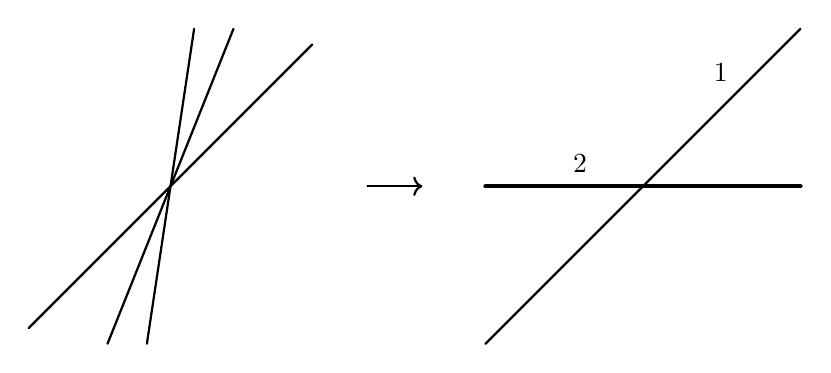
\begin{tikzpicture}[line cap=round, line join=round]

  % --- 左侧图形：三条交汇的直线 ---
  \begin{scope}
    % 最平缓的线
    \draw[thick] (-1.8, -1.8) -- (1.8, 1.8);
    % 中间坡度的线
    \draw[thick] (-0.8, -2)   -- (0.8, 2);
    % 最陡的线
    \draw[thick] (-0.3, -2)   -- (0.3, 2);
  \end{scope}

  % --- 中间的箭头 ---
  \draw[->, thick] (2.5, 0) -- (3.2, 0);

  % --- 右侧图形：水平线和斜线 ---
  \begin{scope}[shift={(6,0)}]
    % 加粗的水平线
    \draw[ultra thick] (-2, 0) -- (2, 0);
    % 斜线
    \draw[thick] (-2, -2) -- (2, 2);

    % 标注数字 2 (在水平线上方)
    \node[above] at (-0.8, 0.05) {2};
    % 标注数字 1 (在斜线上方)
    \node[above left] at (1.2, 1.2) {1};
  \end{scope}

\end{tikzpicture}
\end{center}


对更一般的曲线, 想法相同.

\subsection*{Kodaira 的工作}

在考虑 N\'eron 模型之前, 我们考察一个类似的情形, 即它的先驱. 考虑方程
\[
Y^2Z = X^3 + a(T)XZ^2 + b(T)Z^3, \qquad
\Delta(T) \mathrel{=_{\mathrm{def}}} 4a(T)^3 + 27b(T)^2\neq 0,
\]
其中 $a(T), b(T)\in\mathbb{C}[T]$. 可把它视为定义三个不同对象:
\begin{enumerate}[label=\textup{(\alph*)}]
\item 域 $\mathbb{C}(T)$ 上的椭圆曲线 $E$;
\item $\mathbb{P}^2(\mathbb{C})\times\mathbb{A}^1(\mathbb{C})$ 中的曲面 $S$, 其点是满足方程的序对 $((x:y:z), t)$;
\item 由 $T$ 参数化的 (可能退化的) 椭圆曲线族 $E(T)$.
\end{enumerate}
(c) 的含义如下: 对每个 $t_0\in\mathbb{C}$, 有曲线
\[
E(t_0)\colon Y^2Z = X^3 + a(t_0)XZ^2 + b(t_0)Z^3, \qquad a(t_0), b(t_0)\in\mathbb{C},
\]
带判别式 $\Delta(t_0)$. 当且仅当 $t_0$ 不是多项式 $\Delta(T)$ 的根时它非奇异, 从而是椭圆曲线; 否则它有奇点, 我们把它视为退化椭圆曲线. 注意投影 $\mathbb{P}^2(\mathbb{C})\times\mathbb{A}^1(\mathbb{C})\to\mathbb{A}^1(\mathbb{C})$ 诱导映射 $S\to\mathbb{A}^1(\mathbb{C})$, 其纤维\index{xianwei@纤维(fibre)}正是曲线 $E(t)$. 可把 $S$ 视为 $E$ 在 $\mathbb{C}[T]$ 上 (或 $\mathbb{A}^1(\mathbb{C})$ 上) 的``模型''. 我们应选取 $E$ 的方程使 $\Delta(T)$ 的次数尽可能小, 从而使奇异纤维尽可能少.

为方便, 现在省去 $Z$, 考虑方程
\[
S\colon Y^2 = X^3 + a(T)X + b(T), \qquad a(T), b(T)\in\mathbb{C}[T].
\]
(严格地说, 我们应在射影曲线族上工作.)

设 $P = (x,y,t)\in S(\mathbb{C})$, 令 $f(X,Y,T) = X^3 + a(T)X + b(T) - Y^2$. 则 $P$ 在曲线 $E(t)$ 上奇异当且仅当它满足方程
\[
\frac{\partial f}{\partial Y} = -2Y = 0, \qquad
\frac{\partial f}{\partial X} = 3X^2 + a(T) = 0.
\]
若此外它满足方程
\[
\frac{\partial f}{\partial T} = \frac{da}{dT}X + \frac{db}{dT} = 0,
\]
则它在曲面 $S$ 上奇异. 故 $P$ 可能在纤维 $E(t)$ 中奇异, 而不在 $S$ 上奇异.

\begin{example} \label{thm:2.7.1} 
\begin{enumerate}[label=\textup{(\alph*)}]
\item 考虑方程 $Y^2 = X^3 - T$, $\Delta(T) = 27T^2$. 原点视为曲线 $E(0)\colon Y^2 = X^3$ 上的点时奇异 (事实上是尖点), 但视为曲面 $S\colon Y^2 = X^3 - T$ 上的点时却不奇异. 事实上, $S$ 在原点的切平面是 $(X,Y)$-平面 $T = 0$.
\item 考虑方程 $Y^2 = X^3 - T^2$, $\Delta(T) = 27T^4$. 此时原点视为 $E(0)$ 上的点时奇异, 视为 $S$ 上的点也奇异.
\item 考虑方程
\[
Y^2 = (X - 1 + T)(X - 1 - T)(X + 2) = X^3 - (3 + T^2)X + 2 - 2T^2.
\]
判别式为 $\Delta(T) = -324T^2 + 72T^4 - 4T^6$. 曲线 $E(0)$ 是
\[
Y^2 = X^3 - 3X + 2 = (X-1)^2(X+2),
\]
在 $(1,0)$ 处有结点. 为把 $(1,0,0)$ 平移到原点, 在原方程中用 $X$ 替换 $X - 1$, 方程变为
\[
Y^2 = (X + T)(X - T)(X + 3) = (X^2 - T^2)(X + 3) = X^3 + 3X^2 - T^2X - 3T^2.
\]
此曲面在原点处有奇点, 因为其方程没有线性项.
\end{enumerate}
\end{example}

\cite{kodaira1960} 表明, 通过吹胀 (blowing up) 点、吹缩 (blowing down) 曲线等, 可以从曲面
\[
S\colon Y^2Z = X^3 + a(T)XZ^2 + b(T)Z^3, \qquad a(T), b(T)\in\mathbb{C}[T], \ \Delta(T)\neq 0
\]
得到新曲面 $S_0$ 与正则映射 $S_0\to\mathbb{A}^1$, 具有以下性质:
\begin{enumerate}[label=\textup{(\alph*)}]
\item $S_0$ 非奇异;
\item 把 $S_0$ 视为 $\mathbb{C}(T)$ 上的曲线等于把 $S$ 视为 $\mathbb{C}(T)$ 上的曲线 (对专家: 映射 $S\to\mathbb{A}^1$ 与 $S_0\to\mathbb{A}^1$ 有相同的普通纤维);
\item $S_0$ 在 $\mathbb{A}^1(\mathbb{C})$ 之上的纤维 $E'(t_0)$ 是射影曲线; 且若 $E(t_0)$ 的点视为 $S$ 上的点时非奇异 (例如 $E(t_0)$ 本身非奇异), 则 $E'(t_0) = E(t_0)$;
\item $S_0$ 关于上述性质极小: 若 $S''\to\mathbb{A}^1$ 是具有性质 (a,b,c) 的第二个映射, 则在普通纤维上是同构的每个正则映射 $S_0\to S''$ (在 $\mathbb{A}^1$ 上) 都是同构.
\end{enumerate}
映射 $S_0\to\mathbb{A}^1$ 由这些性质在唯一同构的意义下唯一确定. Kodaira 分类了 $S_0\to\mathbb{A}^1$ 的可能纤维.

``吹胀''曲面 $S$ 的非奇异点 $P$ 保持曲面不变, 只是把点 $P$ 换成 $S$ 在 $P$ 处切平面中过原点的直线射影空间. 对过 $P$ 的曲线 $C$, $C\setminus\{P\}$ 的逆像是吹胀簇中的曲线, 其闭包在射影空间中交于对应 $C$ 在 $P$ 处切线方向的那一点. 即使 $S\subset\mathbb{P}^m$, 吹胀后的曲面也没有自然嵌入射影空间.

\begin{example} \label{thm:2.7.2} 
为说明``吹胀''现象, 考虑映射
\[
\psi\colon k^2\to k^2, \qquad (x,y)\mapsto(x, xy).
\]
它的像只遗漏 $Y$-轴上 $Y\neq 0$ 的点. 像中的点除 $(0,0)$ 外都是 $k^2$ 中唯一点的像, 而 $(0,0)$ 被``吹胀''成整个 $Y$-轴. 换言之, 该映射一对一, 只是 $Y$-轴被``吹缩''成一点. 直线 $L\colon Y = \alpha X$ 的逆像是 $XY = \alpha X$, 它是 $Y$-轴与直线 $Y = \alpha$ 的并; $L\setminus\{(0,0)\}$ 的逆像的闭包是直线 $Y = \alpha$. 奇异曲线
\[
C\colon Y^2 = X^3 + \alpha X^2
\]
的逆像是曲线
\[
Y^2X^2 = X^3 + \alpha X^2,
\]
它是曲线 $X^2 = 0$ (``重数''为 $2$ 的 $Y$-轴) 与非奇异曲线 $Y^2 = X + \alpha$ 的并. 注意后者与 $Y$-轴交于点 $(0,\pm\sqrt{\alpha})$, 即对应 $C$ 在 $(0,0)$ 处切线的斜率的那两点.

此例中, $\mathbb{A}^2(k)$ 中的 $(0,0)$ 被吹胀成一条仿射直线. 在真正的吹胀中, 它将被换成一条射影直线, 且映射的描述更复杂. ($\mathbb{P}^2$ 中点的吹胀见 \cite[Chap. 7]{fulton1969}.)
\end{example}

\subsection*{N\'eron 的工作}

N\'eron 对 $\mathbb{Q}_p$ 上的椭圆曲线证明了 Kodaira 结果的类似物.\footnote{更准确地说, 他证明了 Kodaira 对离散赋值环 $\mathbb{C}[[T]]$ 上曲线得到的结果, 也适用于剩余域完美的任意完备赋值环上的曲线.} 为解释他的结果, 需要谈论概形. 对非专家, $\mathbb{Z}_p$ 上的概形 $\mathcal{E}$ 不过是由系数在 $\mathbb{Z}_p$ 中的多项式方程族定义的对象. 由相同方程 (视为系数在 $\mathbb{Q}_p$ 中) 定义的对象是 $\mathbb{Q}_p$ 上的簇 $E$, 称为 $\mathcal{E}/\mathbb{Z}_p$ 的普通纤维 (generic fibre); 由把系数模 $p$ 的方程定义的对象是 $\mathbb{F}_p$ 上的簇 $\tilde{E}$, 称为 $\mathcal{E}/\mathbb{Z}_p$ 的特殊纤维\index{xianwei@纤维(fibre)!teshu@特殊(special)} (special fibre). 例如, 若 $\mathcal{E}$ 是由方程
\[
Y^2Z + a_1XYZ + a_3YZ^2 = X^3 + a_2X^2Z + a_4XZ^2 + a_6Z^3, \qquad a_i\in\mathbb{Z}_p
\]
定义的概形, 则 $E$ 是由相同方程定义的 $\mathbb{Q}_p$ 上椭圆曲线, $\tilde{E}$ 是由方程
\[
Y^2Z + \tilde{a}_1XYZ + \tilde{a}_3YZ^2 = X^3 + \tilde{a}_2X^2Z + \tilde{a}_4XZ^2 + \tilde{a}_6Z^3
\]
定义的 $\mathbb{F}_p$ 上椭圆曲线, 其中 $\tilde{a}_i$ 是 $a_i$ 在 $\mathbb{Z}/p\mathbb{Z} = \mathbb{F}_p$ 中的像.

给定椭圆曲线 $E/\mathbb{Q}_p$, N\'eron 构造具有如下性质的 $\mathbb{Z}_p$ 上概形 $\mathcal{E}$:
\begin{enumerate}[label=\textup{(\alph*)}]
\item $\mathcal{E}$ 正则 (regular), 即所有相伴局部环都是正则局部环 (若局部环维数为 $d$, 则其极大理想可由 $d$ 个元素生成). (对代数闭域上的代数簇, ``正则''等价于``非奇异''.)
\item $\mathcal{E}$ 的普通纤维是原来的曲线 $E$;
\item $\mathcal{E}$ 在 $\mathbb{Z}_p$ 上真 (proper), 即 $\tilde{E}$ 是射影曲线;
\item $\mathcal{E}$ 关于上述性质极小: 若 $\mathcal{E}'$ 是 $\mathbb{Z}_p$ 上具有性质 (a,b,c) 的第二个概形, 则在普通纤维上是同构的每个 $\mathbb{Z}_p$ 上正则映射 $\mathcal{E}\to\mathcal{E}'$ 都是同构.
\end{enumerate}
且 N\'eron 分类了 $\mathbb{F}_p^{\mathrm{al}}$ 上可能的特殊纤维, 得到与 Kodaira 本质上相同的列表.

$\mathbb{Z}_p$ 上的曲线 $\mathcal{E}$ 称为完全 N\'eron (极小) 模型.\index{moxing@模型(model)!wanquan-Neron@完全 N\'eron(complete Néron model)} 它有些缺点: 未必有 $\mathcal{E}(\mathbb{Z}_p)\cong E(\mathbb{Q}_p)$; 它没有群结构; 其特殊纤维 $\tilde{E}$ 可能奇异. 三个缺点都可通过简单地去掉特殊纤维中的全部奇点与多重曲线来消除. 由此得到光滑 N\'eron (极小) 模型\index{moxing@模型(model)!guanghua-Neron@光滑 N\'eron(smooth Néron model)}, 但它的缺点是不再真.

给定 $\mathbb{Q}_p$ 上的椭圆曲线 $E$, 我们现在在 $\mathbb{Z}_p$ 上有三个模型:
\begin{enumerate}[label=\textup{(\alph*)}]
\item $\mathcal{E}_w$, $E$ 的 Weierstrass 极小模型;
\item $\mathcal{E}$, $E$ 的完全 N\'eron 模型;
\item $\mathcal{E}^0$, $E$ 的光滑 N\'eron 模型.
\end{enumerate}
它们的关系如下: 从 $\mathcal{E}$ 得到 $\mathcal{E}^0$, 需去掉全部多重曲线与奇点; 从 $\mathcal{E}^0$ 得到去掉闭纤维中奇异点的 Weierstrass 模型, 需去掉特殊纤维中除含 $O$ 的分支外的所有连通分支.

\begin{aside} \label{thm:2.7.3} 
按定义, 阿贝尔簇 (abelian variety)\index{abeiercu@阿贝尔簇(abelian variety)} 是带有正则映射定义的群结构的射影代数簇. 故一维阿贝尔簇即椭圆曲线. 椭圆曲线理论的许多 (但非全部) 内容可推广到所有阿贝尔簇, 但因不再能写出方程, 证明需要多得多的代数几何机器. 对维数 $> 1$ 的阿贝尔簇, 只有光滑 N\'eron 极小模型存在.
\end{aside}

\subsection*{不同类型}

我们描述十种 (或按计数方式不同为十一种) 可能模型类型中的三种, 同时使用 Kodaira 编号 ($I_0, I_n, II, \dots$) 与 N\'eron 编号 ($a, b_n, c_1, \dots$). 我们描述 $\mathbb{F}_p$ 的代数闭包而非 $\mathbb{F}_p$ 本身上的特殊纤维. 例如, 在结点约化 (型 $(I_n, b_n)$) 情形, 光滑 N\'eron 模型的特殊纤维的单位连通分支将是 $\mathbb{F}_p$ 上扭的 $\mathbb{G}_m$, 除非切线有理, 且特殊纤维的某些分支在 $\mathbb{F}_p$ 上可能不有理.

\subsection*{($I_0$, a)} 此时 $E$ 有好约化, 三个模型都相同.

\paragraph*{($I_n$, $b_n$), $n>1$} 此时 $E$ 有结点约化; 设 $n = \ord\nolimits_p(\Delta)$; 三个模型的特殊纤维如下:
\begin{enumerate}[label=\textup{(\alph*)}]
\item 带结点的三次曲线;
\item $n$ 条亏格 $0$ 的曲线, 每条恰与另外两条相交;
\item 代数群 $G$, 其单位连通分支 $G^\circ$ 是 $\mathbb{G}_m$, 且 $G/G^\circ$ 是 $n$ 阶循环群.
\end{enumerate}

\begin{center}
\begin{tikzpicture}[line cap=round, line join=round, thick]

  % --- 图 (a): 节点三次曲线 (Nodal Cubic) ---
  \begin{scope}[shift={(0,0)}]
    % 使用参数方程绘制曲线: x = 1 - t^2, y = t(1 - t^2)
    % 调整系数以匹配原图比例
    \draw plot[domain=-1.4:1.4, samples=100] ({-1.5*(\x*\x-1)}, {1.5*\x*(\x*\x-1)});
    \node at (0, -2.5) {(a)};
  \end{scope}

  % --- 图 (b): 带延长线交点的六边形 ---
  \begin{scope}[shift={(5,0)}]
    % 定义六边形的顶点坐标
    \foreach \a [count=\i] in {60, 120, 180, 240, 300, 360} {
      \coordinate (V\i) at (\a:1.3);
    }
    
    % 绘制边，并向两端延长以产生交点效果
    % 这里的 \shorten 是负值，表示向外延长
    \draw[shorten <=-0.3cm, shorten >=-0.3cm] (V1) -- (V2);
    \draw[shorten <=-0.3cm, shorten >=-0.3cm] (V2) -- (V3);
    \draw[shorten <=-0.3cm, shorten >=-0.3cm] (V3) -- (V4);
    \draw[shorten <=-0.3cm, shorten >=-0.3cm] (V4) -- (V5);
    \draw[shorten <=-0.3cm, shorten >=-0.3cm] (V6) -- (V1);
    
    % 图中右下角的边是虚线 (dotted)
    \draw[dotted, shorten <=-0.1cm, shorten >=-0.1cm] (V5) -- (V6);

    \node at (0, -2.5) {(b)};
  \end{scope}

  % --- 图 (c): 文字描述 ---
  \begin{scope}[shift={(9.5,0)}]
    \node[align=center, text width=3cm] at (0,0) {
      相同, 但是没有交点.
    };
    \node at (0, -2.5) {(c)};
  \end{scope}

\end{tikzpicture}
\end{center}

\paragraph*{($I_0^*$, $c_4$)} 此时 $E$ 有尖点约化且 $\ord\nolimits_p(\Delta) = 6$ ($p\neq 2$); 三个模型的特殊纤维如下:
\begin{enumerate}[label=\textup{(\alph*)}]
\item 带尖点的三次曲线;
\item 四条不相交的、重数 $1$ 的亏格 $0$ 曲线, 连同一条重数 $2$、横截穿过四条曲线中每一条的亏格 $0$ 曲线;
\item 代数群 $G$, 其单位连通分支是 $\mathbb{G}_a$, 且 $G/G^\circ$ 是同构于 $\mathbb{Z}/2\mathbb{Z}\times\mathbb{Z}/2\mathbb{Z}$ 的 $4$ 阶群.
\end{enumerate}

\begin{center}
\begin{tikzpicture}[line cap=round, line join=round, thick]

  % --- 图 (a): 尖点曲线 (Cusp Curve) ---
  % 使用参数方程 x = -t^2, y = t^3 来绘制典型的尖点形状
  \begin{scope}[shift={(0,0)}]
    \draw plot[domain=-1.4:1.4, samples=100] ({1.5 - \x*\x}, {0.7*\x*\x*\x});
    \node at (0.5, -2.5) {(a)};
  \end{scope}

  % --- 图 (b): 带有数字标注的相交直线 ---
  \begin{scope}[shift={(5,0)}]
    % 垂直主线
    \draw (0, -1.8) -- (0, 1.8);
    
    % 上方的两条平行斜线 (向下倾斜)
    \draw (-0.8, 1.8) -- (1, 0.8);
    \draw (-0.8, 1.3) -- (1, 0.3);
    
    % 下方的两条平行斜线 (向上倾斜)
    \draw (-0.8, -1.8) -- (1, -0.8);
    \draw (-0.8, -1.3) -- (1, -0.3);
    
    % 数字标注
    \node[above] at (-0.2, 1.4) {1};
    \node[above] at (-0.2, 0.9) {1};
    \node[left]  at (0, 0)   {2};
    \node[above] at (-0.2, -0.8) {1};
    \node[above] at (-0.2, -1.4) {1};

    \node at (0.1, -2.5) {(b)};
  \end{scope}

  % --- 图 (c): 多行文字说明 ---
  \begin{scope}[shift={(9.5,0)}]
    \node[align=center, text width=3.5cm] at (0,0) {
      相同, 但没有多重曲线包括其交点.
    };
    \node at (0, -2.5) {(c)};
  \end{scope}

\end{tikzpicture}
\end{center}

(从 (a) 到 (b) 需去掉重曲线包括其交点; 从 (b) 到 (c) 再去掉.)

使用极小方程时, \S\ref{sec:2.4} 中神秘的商 $E(\mathbb{Q}_p)/E^0(\mathbb{Q}_p)$ 等于 $G(\mathbb{F}_p)/G^\circ(\mathbb{F}_p)$, 其中 $G$ 是光滑 N\'eron 模型的特殊纤维, $G^\circ$ 是 $G$ 的单位连通分支. 在上述三个例子中, 它分别是 (a) 平凡群; (b) $n$ 阶循环群的子群 (若 $E$ 有分裂结点约化则等于 $n$ 阶循环群); (c) $(\mathbb{Z}/2\mathbb{Z})^2$ 的子群.

\subsection*{极小模型的总结}

\begin{center}
\renewcommand{\arraystretch}{1.3}
\begin{tabular}{lccc}
\hline
& Weierstrass & 完全 N\'eron & 光滑 N\'eron\\
\hline
$E$ 是平面曲线 & 是 & 不一定 & 不一定\\
$E$ 正则 & 不一定 & 是 & 是\\
$\tilde{E}$ 射影 & 是 & 是 & 不一定\\
$\tilde{E}$ 非奇异 & 不一定 & 不一定 & 是\\
$\tilde{E}$ 是群 & 不一定 & 不一定 & 是\\
\hline
\end{tabular}
\end{center}

\section{椭圆曲线的算法}\label{sec:2.8}

1965 年前后, Weil 提出 $\mathbb{Q}$ 上固定导子 $N$ 的椭圆曲线与 $\Gamma_0(N)$ 的 $-2$ 维尖点形式之间存在精确对应 (\cite{weil1967}; 见 V, \S\ref{sec:5.5}). 这促使 Tate\footnote{``同一年 (65--66 年), 我从巴黎给 Cassels 写信. 我记得那是在秋天. 那年夏初, Weil 告诉了我所有 $\mathbb{Q}$ 上椭圆曲线都是模曲线的想法. 这激励 Swinnerton-Dyer 对判别式不太大的 $\mathbb{Q}$ 上椭圆曲线做大型计算机搜索, 以检验 Weil 的想法. 但当然必须能计算导子才能做那个检验. 那是我主要的动机. 我不知道为什么我写信给 Cassels 而不是 Swinnerton-Dyer. 也许因为我更了解他.'' Tate, 私人通信.} 找出计算 $\mathbb{Q}$ 上椭圆曲线极小 Weierstrass 方程、判别式、导子、$j$-不变量、N\'eron 模型纤维等的算法, 以便检验 Weil 的想法. 他把它们写进前面提到的给 Cassels 的信中, 即后来发表的 \cite{tate1975}. 这些算法对人类来说痛苦, 但对计算机容易. 幸运的是, 它们已在计算机程序中实现, 例如专门为代数数论 (包括椭圆曲线) 计算设计的 Pari/gp 程序. 下面我解释如何把 Pari 当作超级计算器使用. 也可以编程, 但那需要读手册.

回忆域 $k$ 上椭圆曲线 $E$ 的一般 Weierstrass 方程~\eqref{eq:11} 为
\[
Y^2Z + a_1XYZ + a_3YZ^2 = X^3 + a_2X^2Z + a_4XZ^2 + a_6Z^3,
\]
且依附于曲线量 $b_2, b_4, b_6, b_8, c_4, c_6$ 与
\[
\Delta = -b_2^2b_8 - 8b_4^3 - 27b_6^2 + 9b_2b_4b_6, \qquad j = c_4^3/\Delta.
\]
曲线非奇异当且仅当 $\Delta\neq 0$. 微分形式 $\omega = \frac{dx}{2y + a_1x + a_3}$ 在平移下不变. 椭圆曲线 $E$ 的 Weierstrass 方程在如下坐标变换下确定到唯一:
\[
X = u^2X' + r, \qquad Y = u^3Y' + su^2X' + t, \qquad u,r,s,t\in k, \ u\neq 0.
\]
量 $\Delta$, $j$, $\omega$ 按如下规则变换:
\[
u^{12}\Delta' = \Delta, \qquad j' = j, \qquad \omega' = u\omega.
\]
$\mathbb{Q}$ 上椭圆曲线 $E$ 的极小 Weierstrass 方程是上述形式的、$a_i\in\mathbb{Z}$ 且 $\Delta$ 极小的方程. 它在带 $r,s,t,u\in\mathbb{Z}$, $u\in\mathbb{Z}^{\times} = \{\pm 1\}$ 的上述坐标变换下确定到唯一.

在 gp (grande calculatrice pari) 中, 椭圆曲线由向量
\[
v = [a_1, a_2, a_3, a_4, a_6]
\]
指定.

\begin{center}
\renewcommand{\arraystretch}{1.35}
\begin{tabular}{@{}p{0.38\linewidth}p{\dimexpr0.62\linewidth-2\tabcolsep\relax}@{}}
\texttt{e=ellinit(v,1)} & 把 $e$ 定义为椭圆曲线 $Y^2 + a_1XYZ + \cdots$, 并计算 13 分量向量\\
& $[a_1,\allowbreak a_2,\allowbreak a_3,\allowbreak a_4,\allowbreak a_6,\allowbreak b_2,\allowbreak b_4,\allowbreak b_6,\allowbreak b_8,\allowbreak c_4,\allowbreak c_6,\allowbreak \Delta,\allowbreak j]$\\
\texttt{e=ellinit(v)} & 把 $e$ 定义为椭圆曲线 $Y^2 + a_1XYZ + \cdots$, 并计算上述 13 分量向量\\
& 连同一些对其他计算有用的额外信息\\
\texttt{elladd(e,z1,z2)} & 计算 $e$ 上点 $z_1 = [x_1, y_2]$ 与 $z_2 = [x_2, y_2]$ 的和\\
\texttt{elltors(e)} & 计算 $[t, v_1, v_2]$, 其中 $t$ 是 $E(\mathbb{Q})_{\mathrm{tors}}$ 的阶, $v_1$ 给出\\
& $E(\mathbb{Q})_{\mathrm{tors}}$ 作为循环群乘积的结构, $v_2$ 给出循环群的生成元\\
\texttt{ellglobalred(e)} & 计算向量 $[N, v, c]$, 其中 $N$ 是曲线的导子, $v = [u, r, s, t]$\\
& 是化为 Weierstrass 极小模型的坐标变换 (其中 $a_1 = 0$ 或 $1$, $a_2 = 0, 1, -1$,\\
& $a_3 = 0, 1$). 这样的模型唯一\\
\texttt{e0=ellchangecurve(e,v)} & 把 $e$ 换成 $e_0$, 其中 $e_0$ 是对应于由坐标变换\\
& $v = [u, r, s, t]$ 得到的曲线的 $13{+}$ 分量向量\\
\texttt{ellocalred(e,p)} & 用 Kodaira 记号计算在 $p$ 处约化的类型. 产生 $[f, n, \dots]$,\\
& 其中 $f$ 是 $p$ 在 $e$ 的导子中的指数, $n = 1$ 表示好约化 (型 $I_0$),\\
& $n = 2, 3, 4$ 表示型 $II, III, IV$ 的约化, $n = 4+\nu$ 表示型 $I_\nu$,\\
& $-1, -2$ 等表示 $I_0^*, II^*, \dots$\\
\texttt{ellap(e,p)} & 计算 $a_p \mathrel{=_{\mathrm{def}}} p + 1 - \#E(\mathbb{F}_p)$. 要求 $e$ 在 $p$ 处极小\\
\texttt{ellan(e,n)} & 计算前 $n$ 个 $a_k$. 要求 $e$ 在 $p$ 处极小\\
\texttt{ellgenerators(e)} & 计算 $E(\mathbb{Q})/\mathrm{tors}$ 的基 (要求 John Cremona 的椭圆曲线数据可用)
\end{tabular}
\end{center}

\subsection*{例子 (Example)}

启动 gp.
\begin{verbatim}
gp>  v=[0,-4,0,0,16]
\end{verbatim}
把 $v$ 设为向量 $(0,-4,\dots)$.
\begin{verbatim}
%1 = [0,-4,0,0,16]
gp>  ellinit(v,1)
\end{verbatim}
计算向量 $(a_1,\dots,j)$.
\begin{verbatim}
%2 = [0,-4,0,0,16,-16,0,64,-256,256,-9728,-45056,-4096/11]
\end{verbatim}
例如, $\Delta = -45056$, $j = -4096/11$.
\begin{verbatim}
gp>  e=ellinit(v)
\end{verbatim}
计算向量 $(a_1,\dots,j,\dots)$, 并把 $e$ 设为椭圆曲线 $Y^2 = X^3 - 4X^2 + 16$.
\begin{verbatim}
%3 = [0,-4,0,0,16,...]
gp>  elltors(e)
\end{verbatim}
计算挠子群 (它是 $5$ 阶循环群).
\begin{verbatim}
%4 = [5,[5],[0,4]]
gp>  ellglobalred(e)
\end{verbatim}
计算最小导子与给出极小方程所需的坐标变换.
\begin{verbatim}
%5 = [11, [2,0,0,4], 1]
gp>  ellchangecurve(e,[2,0,0,4])
%6 = [0,-1,1,0,0,-4,0,1,-1,16,-152,-11,-4096/11,...]
\end{verbatim}
计算 $E$ 的极小方程 $Y^2 + Y = X^3 - X^2$, 它现在有判别式 $-11$, 但 (当然) 相同的 $j$-不变量.
\begin{verbatim}
gp>  elllocalred(%6,2)
%7 = [0,1,[1,0,0,0],1]
\end{verbatim}
所以 $E$ 现在在 $2$ 处有好约化.
\begin{verbatim}
gp>  elllocalred(%6,11)
%8 = [1,5,[1,0,0,0],1]
\end{verbatim}
所以 $E$ 在 $11$ 处有坏约化, 导子为 $11^1$ (故奇点是结点), 且 N\'eron 模型特殊纤维的 Kodaira 型是 $I_1$.
\begin{verbatim}
gp>  ellap(%6,13)
\end{verbatim}
计算 $a_{13}$.
\begin{verbatim}
%9 = 4
\end{verbatim}
所以 $\#E(\mathbb{F}_{13}) = 13 + 1 - 4 = 10$.
\begin{verbatim}
gp>  ellgenerators(e)
%10 = []
\end{verbatim}
所以 $E(\mathbb{Q})$ 有限.
\begin{verbatim}
gp>  ellinit([6,-3,9,-16,-14])
%11 = [6,-3,9,-16,-14,24,22,25,29,48,-216,37,110592/37,...]
gp>  ellgenerators(%11)
%12 = [[-2,2]]
\end{verbatim}
所以 $E(\mathbb{Q})/\mathrm{tors}$ 是由 $(-2,2)$ 生成的秩 $1$ 自由模.

{\emergencystretch=3em Pari/gp 可从 \url{https://pari.math.u-bordeaux.fr/} 免费获取. 推荐以下资料: 书 \cite{cohen1993}、\cite{cohen2000} 与 \cite{cremona1997}; 数据库 \textit{The L-functions and Modular Forms Database} (\url{https://www.lmfdb.org/}); 文章 \cite{best2020}.\par}

\chapter{复数域上的椭圆曲线}\label{ch:3}

\begin{quote}\small\itshape
基域为 $\mathbb{C}$ 的情形正是经典的椭圆函数理论，这一理论可见于任何一本足够传统的分析学教科书.
\end{quote}
\vspace{-0.5em}
\hfill \small \cite{cassels1966}.

当基域为复数域时, 椭圆曲线的理论大为简化.

\section{格与基}\label{sec:3.1}

$\mathbb{C}$ 中的格 (lattice)\index{ge@格(lattice)} 是由两个在 $\mathbb{R}$ 上线性无关的复数生成的子群. 故
\[
\Lambda = \mathbb{Z}\omega_1 + \mathbb{Z}\omega_2, \qquad \text{某些 } \omega_1, \omega_2\in\mathbb{C},
\]
且因 $\omega_1$ 与 $\omega_2$ 互不为实倍数, 可把它们排序使 $\Im(\omega_1/\omega_2) > 0$. 若 $\{\omega_1', \omega_2'\}$ 是 $\Lambda$ 的第二对元素, 则
\[
\omega_1' = a\omega_1 + b\omega_2, \qquad \omega_2' = c\omega_1 + d\omega_2, \qquad \text{某些 } a, b, c, d\in\mathbb{Z},
\]
即
\[
\begin{pmatrix}\omega_1'\\ \omega_2'\end{pmatrix} = A\begin{pmatrix}\omega_1\\ \omega_2\end{pmatrix},
\]
其中 $A$ 是整系数 $2\times 2$ 矩阵. 序对 $(\omega_1', \omega_2')$ 是 $\Lambda$ 的 $\mathbb{Z}$-基当且仅当 $A$ 可逆, 从而行列式为 $\pm 1$. 令 $z = \omega_1/\omega_2$, $z' = \omega_1'/\omega_2'$, 则
\[
\Im(z') = \Im\Bigl(\frac{az+b}{cz+d}\Bigr) = \frac{\Im(adz + bc\bar{z})}{|cz+d|^2} = \frac{(ad-bc)\Im(z)}{|cz+d|^2},
\]
故 $\Im(\omega_1'/\omega_2') > 0$ 当且仅当 $\det A > 0$. 因此, 整系数行列式为 $1$ 的矩阵群 $\mathrm{SL}_2(\mathbb{Z})$ 传递地作用在 $\Lambda$ 的满足 $\Im(\omega_1/\omega_2) > 0$ 的基集上. 我们证明了以下陈述.

\begin{proposition} \label{thm:3.1.1} 
设 $M$ 为满足 $\Im(\omega_1/\omega_2) > 0$ 的复数对 $(\omega_1, \omega_2)$ 的集合, $L$ 为 $\mathbb{C}$ 中格的集合. 则映射 $(\omega_1, \omega_2)\mapsto\mathbb{Z}\omega_1 + \mathbb{Z}\omega_2$ 诱导双射
\begin{equation} \label{eq:19}
\mathrm{SL}_2(\mathbb{Z})\setminus M \to L.
\tag{19}
\end{equation}
\end{proposition}

这里 $\mathrm{SL}_2(\mathbb{Z})\setminus M$ 表示 $M$ 在如下作用下的轨道集:
\[
\begin{pmatrix}a & b\\ c & d\end{pmatrix}\begin{pmatrix}\omega_1\\ \omega_2\end{pmatrix} = \begin{pmatrix}a\omega_1 + b\omega_2\\ c\omega_1 + d\omega_2\end{pmatrix}.
\]

设 $\mathbb{H}$ 为复上半平面:
\[
\mathbb{H} = \{z\in\mathbb{C} \mid \Im(z) > 0\}.
\]
令 $z\in\mathbb{C}^{\times}$ 按规则 $z(\omega_1, \omega_2) = (z\omega_1, z\omega_2)$ 作用在 $M$ 上, 按规则 $z\Lambda = \{z\lambda \mid \lambda\in\Lambda\}$ 作用在 $L$ 上. 映射 $(\omega_1, \omega_2)\mapsto\omega_1/\omega_2$ 诱导双射
\begin{equation} \label{eq:20}
M/\mathbb{C}^{\times}\to\mathbb{H}.
\tag{20}
\end{equation}
$\mathrm{SL}_2(\mathbb{Z})$ 在 $M$ 上的作用对应于它在 $\mathbb{H}$ 上的作用
\[
\begin{pmatrix}a & b\\ c & d\end{pmatrix}\tau = \frac{a\tau + b}{c\tau + d}.
\]
合并 \eqref{eq:19} 与 \eqref{eq:20}, 得双射
\[
\begin{array}{ccccc}
L/\mathbb{C}^{\times} & & \mathrm{SL}_2(\mathbb{Z})\setminus M/\mathbb{C}^{\times} & & \mathrm{SL}_2(\mathbb{Z})\setminus\mathbb{H}\\
(\mathbb{Z}\omega_1 + \mathbb{Z}\omega_2)\mathbb{C}^{\times} & \longleftrightarrow & \mathrm{SL}_2(\mathbb{Z})\cdot(\omega_1, \omega_2)\mathbb{C}^{\times} & \longleftrightarrow & \mathrm{SL}_2(\mathbb{Z})\cdot\frac{\omega_1}{\omega_2}.
\end{array}
\]

对具有基 $\{\omega_1, \omega_2\}$ 的格 $\Lambda$, 以 $z_0$, $z_0+\omega_1$, $z_0+\omega_2$, $z_0+\omega_1+\omega_2$ 为顶点的任何平行四边形的内部称为 $\Lambda$ 的基本区域 (fundamental domain)\index{jibenyu@基本域(fundamental domain)} 或周期平行四边形 (period parallelogram).\index{zhouqipingxingsibianxing@周期平行四边形(period parallelogram)} 通常选取 $z_0$ 使该区域包含 $0$.

\section{双周期函数}\label{sec:3.2}

设 $\Lambda$ 为 $\mathbb{C}$ 中的格. 给出 $\mathbb{C}/\Lambda$ 上的函数等价于给出 $\mathbb{C}$ 上满足
\begin{equation} \label{eq:21}
f(z+\lambda) = f(z) \qquad (\text{作为 } \mathbb{C} \text{ 上的函数})
\tag{21}
\end{equation}
(对所有 $\lambda\in\Lambda$) 的函数 $f$. 若 $\{\omega_1, \omega_2\}$ 是 $\Lambda$ 的基, 则此条件等价于
\[
\begin{cases}
f(z+\omega_1) = f(z)\\
f(z+\omega_2) = f(z).
\end{cases}
\]
为此, 满足 \eqref{eq:21} 的函数称为双周期的 (doubly periodic).\index{hanshu@函数(function)!shuangzhouqi@双周期(doubly periodic)} 本节研究 $\mathbb{C}$ 上对格 $\Lambda$ 双周期亚纯的函数, 下节把这些函数解释为商 Riemann 曲面 $\mathbb{C}/\Lambda$ 上的亚纯函数\index{hanshu@函数(function)!yachun@亚纯(meromorphic)}.

\begin{proposition} \label{thm:3.2.1} 
设 $f(z)$ 为对 $\Lambda$ 双周期、不恒为零的亚纯函数, $D$ 为 $\Lambda$ 的基本域, 且 $f$ 在 $D$ 的边界上无零点或极点. 则
\begin{enumerate}[label=\textup{(\alph*)}]
\item $\sum\limits_{P\in D}\operatorname{Res}_P(f) = 0$;
\item $\sum\limits_{P\in D}\operatorname{ord}_P(f) = 0$;
\item $\sum\limits_{P\in D}\operatorname{ord}_P(f)\cdot P\equiv 0 \pmod{\Lambda}$.
\end{enumerate}
第一个和遍历 $D$ 中 $f$ 有极点的点, 其他和遍历 $f$ 有零点或极点的点 ($\operatorname{ord}_P(f)$ 是零点的阶或极点的负阶). 每个和都有限.
\end{proposition}

\begin{proof}
由留数定理 (\cite[III, 5.2]{cartan1963}),
\[
\int_{\partial D} f(z)\,dz = 2\pi i\sum\limits_{P\in D}\operatorname{Res}_P(f),
\]
其中 $\partial D$ 是 $D$ 的边界. 因 $f$ 周期, $D$ 对边的积分抵消, 故积分为零. 这给出 (a). 对 (b), 把留数定理应用于 $f'/f$, 注意它仍双周期且 $\operatorname{Res}_P(f'/f) = \operatorname{ord}_P(f)$. 对 (c), 把留数定理应用于 $z\cdot f'(z)/f(z)$. 它不再双周期, 但它绕 $\partial D$ 的积分属于 $\Lambda$.
\end{proof}

\begin{corollary} \label{thm:3.2.2} 
非常数的双周期亚纯函数至少有两个极点 (或一个二重极点).
\end{corollary}

\begin{proof}
全纯的双周期函数在任何基本域的闭包上有界 (由紧致性), 从而在整个平面上有界 (由周期性). 由 Liouville 定理 (\cite[III, 1.2]{cartan1963}), 它是常数. 双周期亚纯函数不可能在周期平行四边形中只有一个单极点, 因为由命题的 (a), 该极点处的留数必须为零, 从而该极点不是单极点.
\end{proof}

\subsection*{Weierstrass $\wp$ 函数}

设 $\Lambda$ 为 $\mathbb{C}$ 中的格. 把 Riemann--Roch 定理应用于商 $\mathbb{C}/\Lambda$ 可证明 $\Lambda$ 的非常数双周期亚纯函数的存在性, 但这里我们显式地构造它们. 当 $G$ 是作用在集合 $S$ 上的有限群时, 构造在 $G$ 作用下不变的函数很容易: 取任意函数 $f\colon S\to\mathbb{C}$, 定义
\[
F(s) = \sum\limits_{g\in G} f(gs);
\]
则 $F(g_0s) = \sum\limits_{g\in G} f(g_0gs) = F(s)$, 因为当 $g$ 遍历 $G$ 时 $g_0g$ 也遍历 $G$; 故 $F$ 不变, 且 (显然) 所有不变函数都有此形式. 当 $G$ 不有限时, 必须验证级数收敛——事实上, 为使结果与求和次序无关, 需要 (至少) 绝对收敛.

设 $D$ 为 $\mathbb{C}$ 的开子集, $f_0, f_1, \dots$ 为 $D$ 上的全纯函数序列. 回忆 (\cite[I, 2]{cartan1963}) 级数 $\sum\limits_n f_n$ 称为在 $D$ 的子集 $A$ 上正规收敛\index{zhengguishoulian@正规收敛(converge normally)} (normally convergent), 若正项级数 $\sum\limits_n\|f_n\|$ 收敛, 其中 $\|f_n\| = \sup_{z\in A}|f_n(z)|$. 级数 $\sum\limits_n f_n$ 于是 在 $A$ 上一致且绝对收敛. 当 $f_0, f_1, \dots$ 是亚纯函数序列时, 称级数在 $A$ 上正规收敛, 若去掉有限多个项 $f_n$ 后变成全纯函数的正规收敛级数 (\cite[V, 2]{cartan1963}). 若亚纯函数级数 $\sum\limits_n f_n$ 在 $D$ 的紧子集上正规收敛, 则其和 $f$ 是 $D$ 上的亚纯函数; 且导数级数在 $D$ 的紧子集上正规收敛, 其和是 $f$ 的导数 (\cite[V, 2]{cartan1963}).

现在设 $\varphi(z)$ 为 $\mathbb{C}$ 上的亚纯函数, 令
\[
\Phi(z) = \sum\limits_{\omega\in\Lambda}\varphi(z+\omega).
\]
假设当 $|z|\to\infty$ 时 $\varphi(z)\to 0$ 足够快, 使 $\Phi(z)$ 的级数在紧子集上正规收敛. 则 $\Phi(z)$ 关于 $\Lambda$ 双周期, 因为把 $z$ 换成 $z+\omega_0$ ($\omega_0\in\Lambda$) 只是重排求和中的项.

为证明我们感兴趣函数的正规收敛, 需要下面的结果.

\begin{lemma} \label{thm:3.2.3} 
对 $\mathbb{C}$ 中每个格 $\Lambda$, 级数 $\sum\limits_{\omega\in\Lambda, \omega\neq 0}1/|\omega|^3$ 收敛.
\end{lemma}

\begin{proof}
设 $\omega_1, \omega_2$ 为 $\Lambda$ 的基, 对每个整数 $n\ge 1$, 考虑平行四边形
\[
P(n) = \{a_1\omega_1 + a_2\omega_2 \mid a_1, a_2\in\mathbb{R}, \max(|a_1|, |a_2|) = n\}.
\]
$P(n)$ 上有 $8n$ 个 $\Lambda$ 的点, 且 $0$ 与其中任一点的距离至少为 $kn$, 其中 $k$ 是 $0$ 到 $P(1)\cap\Lambda$ 中点的最短距离. 因此, $P(n)$ 上的点对求和的贡献以 $8n/k^3n^3$ 为界, 故
\[
\sum\limits_{\omega\in\Lambda, \omega\neq 0}\frac{1}{|\omega|^3}\le\frac{8}{k^3}\sum\limits_n\frac{1}{n^2} < \infty.
\]
\end{proof}

由~\ref{thm:3.2.2} 我们知道, 最简单的非常数双周期亚纯函数是在 $\Lambda$ 的每一点有二重极点且无其他极点的函数. 设 $f(z)$ 是这样的函数. 则 $f(z) - f(-z)$ 双周期, 除在 $\Lambda$ 的点处可能有单极点外无其他极点. 故它必为常数, 且因它是奇函数必为零. 于是 $f(z)$ 偶, 且可通过归一化条件使唯一:
\[
f(z) = z^{-2} + 0 + z^2g(z),
\]
其中 $g(z)$ 在 $z = 0$ 附近全纯. 存在这样的函数, 即 Weierstrass 函数 $\wp(z)$, 但不能直接用本小节开头的方法从 $1/z^2$ 定义它, 因为 $\sum\limits_{\omega\in\Lambda}1/(z+\omega)^2$ 不正规收敛. 取而代之, 我们定义
\begin{align*}
\wp(z) &= \frac{1}{z^2} + \sum\limits_{\omega\in\Lambda, \omega\neq 0}\Bigl(\frac{1}{(z-\omega)^2} - \frac{1}{\omega^2}\Bigr),\\
\wp'(z) &= \sum\limits_{\omega\in\Lambda}\frac{-2}{(z-\omega)^3}.
\end{align*}

\begin{proposition} \label{thm:3.2.4} 
上述两级数在 $\mathbb{C}$ 的紧子集上正规收敛, 且其和 $\wp$ 与 $\wp'$ 是 $\mathbb{C}$ 上的双周期亚纯函数, 且 $\wp' = \frac{d\wp}{dz}$.
\end{proposition}

\begin{proof}
注意 $\wp'(z) = \sum\limits_{\omega\in\Lambda}\varphi(z+\omega)$, 其中 $\varphi(z) = \frac{-2}{z^3} = \frac{d}{dz}\bigl(\frac{1}{z^2}\bigr)$, 而级数 $\sum\limits_{\omega\in\Lambda}\varphi(z+\omega)$ 通过与 $\sum 1/|\omega|^3$ 比较在任何紧圆盘 $|z|\le r$ 上正规收敛. 因此由上面的说明, $\wp'(z)$ 是 $\mathbb{C}$ 上的双周期亚纯函数.

对 $|z|\le r$, 除有限多个满足 $|\omega|\le 2r$ 的 $\omega$ 外, 有
\[
\Bigl|\frac{1}{(z-\omega)^2} - \frac{1}{\omega^2}\Bigr|
= \Bigl|\frac{-z^2 + 2\omega z}{\omega^2(z-\omega)^2}\Bigr|
= \frac{|z|\,|2 - \frac{z}{\omega}|}{|\omega|^3\,|1 - \frac{z}{\omega}|^2}
\le \frac{r\cdot\frac{5}{2}}{|\omega|^3\cdot\frac{1}{4}} = \frac{10r}{|\omega|^3},
\]
故 $\wp(z)$ 也在紧圆盘 $|z|\le r$ 上正规收敛. 因其导数双周期, $\wp(z)$ 也双周期.
\end{proof}

\subsection*{Eisenstein 级数}

设 $\Lambda$ 为 $\mathbb{C}$ 中的格, 考虑和
\[
\sum\limits_{\omega\in\Lambda, \omega\neq 0}\frac{1}{\omega^n}.
\]
映射 $\omega\mapsto-\omega\colon\Lambda\to\Lambda$ 的阶为 $2$, 其唯一不动点是 $0$. 故 $\Lambda\setminus\{0\}$ 是其轨道的无交并, 由此推出 $n$ 为奇数时该和为零. 我们写
\[
G_{2k}(\Lambda) = \sum\limits_{\omega\in\Lambda, \omega\neq 0}\frac{1}{\omega^{2k}},
\]
并令 $G_{2k}(z) = G_{2k}(\mathbb{Z}z + \mathbb{Z})$, $z\in\mathbb{H}$. 注意对 $c\in\mathbb{C}^{\times}$ 有
\[
G_{2k}(c\Lambda) = c^{-2k}G_{2k}(\Lambda),
\]
故 $G_{2k}(\mathbb{Z}\omega_1 + \mathbb{Z}\omega_2) = \omega_2^{-2k}G_{2k}(\mathbb{Z}\frac{\omega_1}{\omega_2} + \mathbb{Z})$.

\begin{proposition} \label{thm:3.2.5} 
对所有整数 $k\ge 2$, $G_{2k}(z)$ 收敛到 $\mathbb{H}$ 上的全纯函数.
\end{proposition}

\begin{proof}
设
\[
D = \{z\in\mathbb{C} \mid |z|\ge 1, \ |\Re(z)|\le 1/2\}.
\]
对 $z\in D$,
\[
|mz + n|^2 = m^2z\bar{z} + 2mn\Re(z) + n^2\ge m^2 - mn + n^2 = |m\rho - n|^2,
\]
其中 $\rho = e^{2\pi i/3}$. 因此, 引理 \ref{thm:3.2.3} 表明对 $k\ge 2$, $G_{2k}(z)$ 在 $D$ 上正规收敛. 对所有 $A\in\mathrm{SL}_2(\mathbb{Z})$, $G_{2k}(A^{-1}z)$ 也在 $D$ 上正规收敛, 这表明 $G_{2k}(z)$ 在 $AD$ 上正规收敛. 在 V\ref{thm:5.1.3} 中我们将看到集合 $AD$ 覆盖 $\mathbb{H}$, 故这表明 $G_{2k}(z)$ 在整个 $\mathbb{H}$ 上全纯.
\end{proof}

函数 $G_{2k}(\Lambda)$ 与 $G_{2k}(z)$ 称为 Eisenstein 级数.\index{Eisenstein@Eisenstein 级数(Eisenstein series)}

\subsection*{双周期亚纯函数的域}

固定 $\mathbb{C}$ 中的格 $\Lambda$, 令 $\wp(z)$ 为 $\Lambda$ 的 Weierstrass $\wp$ 函数. 对 $\Lambda$ 双周期的函数构成 $\mathbb{C}$ 上亚纯函数域 $M(\mathbb{C})$ 的子域, 我们现在确定它.

\begin{proposition} \label{thm:3.2.6} 
$\wp$ 与 $\wp'$ 之间有关系
\[
\wp'(z)^2 = 4\wp(z)^3 - g_4\wp(z) - g_6,
\]
其中 $g_4 = 60G_4(\Lambda)$, $g_6 = 140G_6(\Lambda)$.
\end{proposition}

\begin{proof}
计算 $\wp(z)$ 在 $0$ 附近的 Laurent 展开. 回忆对 $|t| < 1$,
\[
\frac{1}{1-t} = 1 + t + t^2 + \cdots.
\]
求导, 得
\[
\frac{1}{(1-t)^2} = \sum\limits_{n\ge 1}nt^{n-1} = \sum\limits_{n\ge 0}(n+1)t^n.
\]
故对 $|z| < |\omega|$,
\[
\frac{1}{(z-\omega)^2} - \frac{1}{\omega^2} = \frac{1}{\omega^2}\Bigl(\frac{1}{(1-\frac{z}{\omega})^2} - 1\Bigr) = \sum\limits_{n\ge 1}(n+1)\frac{z^n}{\omega^{n+2}}.
\]
代入 $\wp(z)$ 的定义并交换求和次序, 对 $|z| < |\omega|$ 有
\begin{align*}
\wp(z) &= \frac{1}{z^2} + \sum\limits_{n\ge 1}\sum\limits_{\omega\neq 0}(n+1)\frac{z^n}{\omega^{n+2}}
= \frac{1}{z^2} + \sum\limits_{k\ge 1}(2k+1)G_{2k+2}(\Lambda)z^{2k}\\
&= \frac{1}{z^2} + 3G_4z^2 + 5G_6z^4 + \cdots.
\end{align*}
因此
\[
\wp'(z) = -\frac{2}{z^3} + 6G_4z + 20G_6z^3 + \cdots.
\]
这些表达式包含足够的项, 足以说明
\[
\wp'(z)^2 - 4\wp(z)^3 + 60G_4(\Lambda)\wp(z) + 140G_6(\Lambda)
\]
的 Laurent 展开中没有 $n\le 0$ 的非零 $z^n$ 项. 故该函数在 $0$ 处全纯且取值为 $0$. 由于它双周期且在含 $0$ 的适当基本域中无极点, 我们看到它是常数, 事实上为零.
\end{proof}

\begin{proposition} \label{thm:3.2.7} 
双周期亚纯函数的域是 $M(\mathbb{C})$ 中由 $\wp$ 与 $\wp'$ 生成的子域 $\mathbb{C}(\wp, \wp')$, 即每个双周期亚纯函数都可表示为 $\wp$ 与 $\wp'$ 的有理函数.
\end{proposition}

\begin{proof}
先证每个偶双周期亚纯函数 $f$ 属于 $\mathbb{C}(\wp)$.

观察, 因 $f(z) = f(-z)$, $f$ 的 $k$ 阶导数满足 $f^{(k)}(z) = (-1)^k f^{(k)}(-z)$. 因此, 若 $f$ 在 $z_0$ 处有 $m$ 阶零点, 则它在 $-z_0$ 处有 $m$ 阶零点. 把此说明应用于 $1/f$, 得到``零点''换成``极点''的相同陈述.

类似地, 因 $f^{(2k+1)}(z_0) = -f^{(2k+1)}(-z_0)$, 若 $z_0\equiv-z_0\pmod{\Lambda}$, 则 $f$ 在 $z_0$ 处零点 (或极点) 的阶是偶数.

{\emergencystretch=3em 选 $f$ 在 $\Lambda$ 之外 (且不在 $\Lambda$ 中) 的零点与极点的模 $\Lambda$ 代表元集, 编号为 $z_1, \dots, z_m$, $-z_1, \dots, -z_m$, $z_{m+1}, \dots, z_n$, 使 (模 $\Lambda$)\par}
\[
z_i\not\equiv -z_i \ (1\le i\le m), \qquad z_i\equiv -z_i\not\equiv 0 \ (m < i\le n).
\]
令 $m_i$ 为 $f$ 在 $z_i$ 处的阶; 由第二个观察, 对 $i > m$, $m_i$ 偶. 现在 $\wp(z) - \wp(z_i)$ 也是偶双周期函数. 由于它在基本域中恰有两个极点, 它必在其中恰有两个零点. 当 $i\le m$ 时, 它在 $\pm z_i$ 处有单零点; 当 $i > m$ 时, 它在 $z_i$ 处有二重零点 (由第二个观察). 定义
\[
g(z) = \prod_{i=1}^{m}\bigl(\wp(z) - \wp(z_i)\bigr)^{m_i}\cdot\prod_{i=m+1}^{n}\bigl(\wp(z) - \wp(z_i)\bigr)^{m_i/2}.
\]
则 $f(z)$ 与 $g(z)$ 在不在 $\Lambda$ 上的点处有完全相同的零点与极点. 由~\ref{thm:3.2.1}b, 它们在 $z = 0$ 处也有相同的阶, 故 $f/g$ 全纯且双周期, 从而是常数: $f = cg\in\mathbb{C}(\wp)$.

现在考虑任意双周期亚纯函数 $f$. 可把 $f$ 写成偶与奇双周期函数之和:
\[
f(z) = \frac{f(z) + f(-z)}{2} + \frac{f(z) - f(-z)}{2}.
\]
我们知道偶双周期亚纯函数属于 $\mathbb{C}(\wp)$, 而显然奇双周期亚纯函数属于 $\wp'\cdot\mathbb{C}(\wp)$.
\end{proof}

令
\[
\mathbb{C}[x, y] = \frac{\mathbb{C}[X, Y]}{(Y^2 - 4X^3 + g_4X + g_6)},
\]
{\emergencystretch=3em 并令 $\mathbb{C}[\wp, \wp']$ 为由 $\wp$ 与 $\wp'$ 生成的 $\mathbb{C}$ 上亚纯函数 $\mathbb{C}$-代数. 命题 \ref{thm:3.2.6} 表明映射 $(X, Y)\mapsto(\wp(z), \wp'(z))$ 定义同态\par}
\[
\mathbb{C}[x, y]\to\mathbb{C}[\wp, \wp'],
\]
我们将证明它是同构. 为此, 需证使 $g(\wp, \wp') = 0$ 的 $g(X, Y)\in\mathbb{C}[X, Y]$ 只有那些被 $f(X, Y) \overset{\text{def}}{=} Y^2 - 4X^3 + g_4X + g_6$ 整除的. 由结式理论 (I\ref{thm:1.1.24}), 对任何多项式 $g(X, Y)$, 存在多项式 $a(X, Y)$ 与 $b(X, Y)$ 使
\[
a(X, Y)f(X, Y) + b(X, Y)g(X, Y) = r(X)\in\mathbb{C}[X]
\]
且 $\deg_Y(b) < \deg_Y(f)$. 若 $g(\wp, \wp') = 0$, 则 $r(\wp) = 0$, 但容易看出 $\wp$ 在 $\mathbb{C}$ 上超越 (例如它有无穷多个极点). 故 $r = 0$, 从而 $f(X, Y)$ 整除 $b(X, Y)g(X, Y)$. 因 $f(X, Y)$ 不可约, 它必整除 $b(X, Y)$ 或 $g(X, Y)$. 由次数原因它不能整除 $b$, 故必整除 $g$.

同构 $\mathbb{C}[x, y]\to\mathbb{C}[\wp, \wp']$ 在分式域上诱导同构
\[
\mathbb{C}(x, y)\to\mathbb{C}(\wp, \wp').
\]
故 $\mathbb{C}(x, y)$ 典范同构于 $\Lambda$ 的全部双周期亚纯函数的域.

\section{作为 Riemann 曲面的椭圆曲线}\label{sec:3.3}

\subsection*{Riemann 曲面的概念}

设 $X$ 为连通 Hausdorff 拓扑空间, 具有可数开集基. $X$ 的坐标邻域 (coordinate neighbourhood)\index{zuobiaolinyu@坐标邻域(coordinate neighbourhood)} 是序对 $(U, z)$, 其中 $U\subset X$ 为开集, $z$ 把 $U$ 同胚地映到复平面 $\mathbb{C}$ 的开子集上. 两个坐标邻域 $(U_1, z_1)$ 与 $(U_2, z_2)$ 相容 (compatible), 若函数
\[
z_1\circ z_2^{-1}\colon z_2(U_1\cap U_2)\to z_1(U_1\cap U_2)
\]
及其逆全纯. 坐标邻域族 $(U_i, z_i)_{i\in I}$ 若满足 $X = \bigcup_i U_i$, 且对一切 $(i, j)\in I\times I$, $(U_i, z_i)$ 与 $(U_j, z_j)$ 相容, 则称为坐标覆盖\index{zuobiaofugai@坐标覆盖(coordinate covering)} (coordinate covering). 两个坐标覆盖称为等价的, 若它们的并也是坐标覆盖. 这在坐标覆盖集上定义了等价关系, 等价类称为 $X$ 上的复结构 (complex structure).\index{fujiegou@复结构(complex structure)} 配上复结构的空间 $X$ 称为 Riemann 曲面.\index{Riemann@Riemann 曲面(Riemann surface)}

设 $X$ 为 Riemann 曲面. 开集 $U\subset X$ 上的函数 $f\colon U\to\mathbb{C}$ 称为全纯的 (holomorphic)\index{quanchunyingshe@全纯映射(holomorphic map)}, 若它满足: 对定义复结构的等价类中的一个 (从而每个) 坐标覆盖 $(U_i, z_i)_{i\in I}$, 对一切 $i\in I$, $f\circ z_i^{-1}\colon z_i(U\cap U_i)\to\mathbb{C}$ 全纯.

从 Riemann 曲面 $X$ 到第二个 Riemann 曲面 $X'$ 的映射 $f\colon X\to X'$ 称为全纯的 (holomorphic), 若 $g\circ f$ 在 $X'$ 的开子集上的全纯函数 $g$ 是 (情形下) 全纯的. 为此, 只需对 $X$ 与 $X'$ 的某些坐标覆盖检验: 对 $X$ 中每一点 $P$, 存在 $P$ 的坐标邻域 $(U, z)$ 与 $f(P)$ 的坐标邻域 $(U', z')$ 使 $z'\circ f\circ z^{-1}\colon z(U)\to z'(U')$ 全纯. Riemann 曲面的同构 (isomorphism) 是双射全纯映射.

回忆 $\mathbb{C}$ 的开子集 $U$ 上的亚纯函数 (meromorphic function) 是 $U\setminus\Sigma$ 上的全纯函数 $f$ (其中 $\Sigma\subset U$ 为某离散子集), 它在 $\Sigma$ 的每一点 $a$ 处至多有极点, 即存在 $m$ 使 $(z-a)^mf(z)$ 在 $a$ 的邻域内全纯. Riemann 曲面的开子集上的亚纯函数类似定义. 等价地, 它是从 Riemann 曲面到 Riemann 球面的全纯映射 (\cite[VI, 4.5]{cartan1963}).

\begin{example} \label{thm:3.3.1} 
$\mathbb{C}$ 的每个开子集 $U$ 都是 Riemann 曲面, 只需取单个坐标邻域, 即 $U$ 本身 (映射为恒等 $z$).
\end{example}

\begin{example} \label{thm:3.3.2} 
考虑 $\mathbb{R}^3$ 中的单位球面
\[
S^2\colon X^2 + Y^2 + Z^2 = 1,
\]
设 $P$ 为北极 $(0, 0, 1)$. 从 $P$ 出发的球极投影 (stereographic projection) 是映射
\[
(x, y, z)\mapsto\frac{x + iy}{1 - z}\colon S^2\setminus\{P\}\to\mathbb{C}.
\]
取它为 $S^2$ 的坐标邻域. 从南极出发的球极投影给出第二个坐标邻域. 这两个坐标邻域在 $S^2$ 上定义了复结构, 配上此复结构的 $S^2$ 称为 Riemann 球面 (Riemann sphere).\index{Riemann@Riemann 球面(Riemann sphere)} 另一方面, $\mathbb{P}^1(\mathbb{C})$ 从坐标覆盖
\begin{align*}
\mathbb{P}^1(\mathbb{C}) &= U_0(\mathbb{C})\cup U_1(\mathbb{C}),\\
U_0(\mathbb{C}) &\overset{\text{def}}{=} \{(x:y) \mid x\neq 0\}\cong\mathbb{C}, \qquad
U_1(\mathbb{C}) \overset{\text{def}}{=} \{(x:y) \mid y\neq 0\}\cong\mathbb{C},
\end{align*}
\[
(x:y)\mapsto y/x, \qquad (x:y)\mapsto x/y
\]
获得复结构. 映射 $(x, y, z)\mapsto(x:y:z)\colon S^2\to\mathbb{P}^1(\mathbb{C})$ 是 Riemann 曲面的同构.
\end{example}

\subsection*{Riemann 曲面上的微分形式}

$\mathbb{C}$ 的开子集上的微分形式 (differential one-form) 只是表达式 $\omega = fdz$, 其中 $f$ 为亚纯函数. 给定光滑曲线
\[
t\mapsto z(t)\colon[a, b]\to\mathbb{C}, \qquad [a, b] = \{t\in\mathbb{R} \mid a\le t\le b\},
\]
可作积分
\[
\int_\gamma\omega = \int_a^b f(z(t))\cdot z'(t)\cdot dt\in\mathbb{C}.
\]
现在考虑紧 Riemann 曲面 $X$. 若 $\omega$ 是 $X$ 上的微分形式, $(U_i, z_i)$ 是 $X$ 的坐标邻域, 则 $\omega|_{U_i} = f_i(z_i)dz_i$. 若 $(U_j, z_j)$ 是第二个坐标邻域, 使在 $U_i\cap U_j$ 上 $z_j = w(z_i)$, 则在 $U_i\cap U_j$ 上
\[
f_i(z_i)dz_i = f_j(w(z_i))w'(z_i)dz_i.
\]
因此, 给出 $X$ 上的微分形式等价于给出每个 $U_i$ 上满足重叠处方程的微分形式 $f_idz_i$. 对任何 (实) 曲线 $\gamma\colon I\to X$ 与 $X$ 上的微分形式 $\omega$, 积分 $\int_\gamma\omega$ 有意义.

若微分形式在坐标邻域上由全纯函数 $f$ 的形式 $fdz$ 表示, 则称为全纯的 (holomorphic).

{\emergencystretch=3em 一个重要事实: 亏格 $g$ 的 Riemann 曲面上的全纯微分形式\index{quanchunweifengxingshi@全纯微分形式(holomorphic one-form)}构成维数为 $g$ 的复向量空间 $\Omega^1(X)$.\par}

例如, Riemann 球面 $S$ 亏格为 $0$, 故它应无非零全纯微分形式. 注意 $dz$ 在 $\mathbb{C} = S\setminus\{\text{北极}\}$ 上全纯, 但 $z = 1/z'$ 在 $S\setminus\{\text{极点}\}$ 上, 故 $dz = -\frac{1}{z'^2}dz'$, 在北极处有极点. 因而 $dz$ 不能延拓为整个 $S$ 上的全纯微分形式.

\subsection*{格对 $\mathbb{C}$ 的商}

设 $\Lambda$ 为 $\mathbb{C}$ 中的格. 拓扑上商 $\mathbb{C}/\Lambda$ 同构于 $\mathbb{R}^2/\mathbb{Z}^2$, 它是单孔环面 (甜甜圈的表面). 记 $\pi\colon\mathbb{C}\to\mathbb{C}/\Lambda$ 为商映射. 则 $\mathbb{C}/\Lambda$ 有唯一的复结构使 $\pi$ 是 Riemann 曲面的局部同构. 可描述如下: 对所有 $P\in\mathbb{C}/\Lambda$ 与 $Q\in\pi^{-1}(P)$, 存在 $P$ 的开邻域 $U$ 与 $Q$ 的开邻域 $V$ 使 $\pi|_V\colon V\to U$ 是同胚; 坐标邻域 $(U, (\pi|_V)^{-1}\colon U\to V)$ 构成 $\mathbb{C}/\Lambda$ 的坐标覆盖, 从而定义 $\mathbb{C}/\Lambda$ 上的复结构. 相对于此结构, $\mathbb{C}/\Lambda$ 的开子集 $U$ 上的函数 $\varphi\colon U\to\mathbb{C}$ 全纯 (分别地亚纯), 当且仅当复合 $\varphi\circ\pi\colon\pi^{-1}(U)\to\mathbb{C}$ 按通常意义全纯 (分别地亚纯).

我们将看到, 虽然任意两个商 $\mathbb{C}/\Lambda$, $\mathbb{C}/\Lambda'$ 同胚, 但它们作为 Riemann 曲面同构仅当 $\Lambda' = \alpha\Lambda$ 对某个 $\alpha\in\mathbb{C}^{\times}$.

\subsection*{全纯映射 $\mathbb{C}/\Lambda\to\mathbb{C}/\Lambda'$}

设 $\Lambda$ 与 $\Lambda'$ 为 $\mathbb{C}$ 中的格. 映射 $\pi\colon\mathbb{C}\to\mathbb{C}/\Lambda$ 把 $\mathbb{C}$ 实现为 $\mathbb{C}/\Lambda$ 的万有覆盖空间. 因 $\pi'\colon\mathbb{C}\to\mathbb{C}/\Lambda'$ 同理, 每个使 $\varphi(0) = 0$ 的连续映射 $\varphi\colon\mathbb{C}/\Lambda\to\mathbb{C}/\Lambda'$ 唯一提升为连续映射 $\tilde{\varphi}\colon\mathbb{C}\to\mathbb{C}$ 且 $\tilde{\varphi}(0) = 0$,
\[\begin{tikzcd}
	\CC & \CC \\
	{\CC/\Lambda} & {\CC/\Lambda'}
	\arrow["{\tilde\varphi}", dashed, from=1-1, to=1-2]
	\arrow["\pi"', from=1-1, to=2-1]
	\arrow["{\pi'}", from=1-2, to=2-2]
	\arrow["\varphi", from=2-1, to=2-2]
\end{tikzcd}\]
因 $\pi$ 与 $\pi'$ 是 Riemann 曲面的局部同构, 映射 $\varphi$ 全纯当且仅当 $\tilde{\varphi}$ 全纯.

\begin{proposition} \label{thm:3.3.3} 
设 $\Lambda$ 与 $\Lambda'$ 为 $\mathbb{C}$ 中的格. 满足 $\alpha\Lambda\subset\Lambda'$ 的复数 $\alpha$ 定义了全纯映射
\[
[z]\mapsto[\alpha z]\colon\mathbb{C}/\Lambda\to\mathbb{C}/\Lambda'
\]
(把 $0$ 送到 $0$), 且每个把 $0$ 送到 $0$ 的全纯映射 $\mathbb{C}/\Lambda\to\mathbb{C}/\Lambda'$ 都有此形式 (对唯一的 $\alpha$).
\end{proposition}

\begin{proof}
由上面的说明显然 $\alpha$ 定义全纯映射 $\mathbb{C}/\Lambda\to\mathbb{C}/\Lambda'$. 反之, 设 $\varphi\colon\mathbb{C}/\Lambda\to\mathbb{C}/\Lambda'$ 为全纯映射且 $\varphi(0) = 0$, $\tilde{\varphi}$ 为它到把 $0$ 送到 $0$ 的全纯映射 $\mathbb{C}\to\mathbb{C}$ 的唯一提升. 对每个 $\omega\in\Lambda$, 映射 $z\mapsto\tilde{\varphi}(z+\omega) - \tilde{\varphi}(z)$ 连续且取值于 $\Lambda'\subset\mathbb{C}$; 因 $\mathbb{C}$ 连通而 $\Lambda'$ 离散, 该映射必为常数, 故其导数为零:
\[
\tilde{\varphi}'(z+\omega) = \tilde{\varphi}'(z).
\]
因此 $\tilde{\varphi}'(z)$ 双周期. 因它全纯, 必为常数, 设 $\tilde{\varphi}'(z) = \alpha$ 对所有 $z$. 积分, 得 $\tilde{\varphi}(z) = \alpha z + \beta$, 且 $\beta = \tilde{\varphi}(0) = 0$.
\end{proof}

\begin{corollary} \label{thm:3.3.4} 
Riemann 曲面 $\mathbb{C}/\Lambda$ 与 $\mathbb{C}/\Lambda'$ 同构当且仅当 $\Lambda' = \alpha\Lambda$ 对某个 $\alpha\in\mathbb{C}^{\times}$.
\end{corollary}

\begin{proof}
若 $\mathbb{C}/\Lambda$ 与 $\mathbb{C}/\Lambda'$ 同构, 则每个同构 $\mathbb{C}/\Lambda\to\mathbb{C}/\Lambda'$ 对某个 $\alpha\in\mathbb{C}$ 有 $[z]\mapsto[\alpha z]$ 的形式, 故 $\Lambda' = \alpha\Lambda$. 反之, 若 $\Lambda' = \alpha\Lambda$, 则 $[z]\mapsto[\alpha z]$ 是同构 $\mathbb{C}/\Lambda\to\mathbb{C}/\Lambda'$.
\end{proof}

\begin{corollary} \label{thm:3.3.5} 
每个把 $0$ 送到 $0$ 的全纯映射 $\mathbb{C}/\Lambda\to\mathbb{C}/\Lambda'$ 是群同态.
\end{corollary}

\begin{proof}
显然 $[z]\mapsto[\alpha z]$ 是群同态.
\end{proof}

命题表明
\[
\operatorname{Hom}(\mathbb{C}/\Lambda, \mathbb{C}/\Lambda') \cong \{\alpha\in\mathbb{C} \mid \alpha\Lambda\subset\Lambda'\},
\]
而第一个推论表明有一一对应
\[
\{\mathbb{C}/\Lambda \text{ 模同构}\}\to L/\mathbb{C}^{\times}.
\]

\subsection*{椭圆曲线 $E(\Lambda)$}

设 $\Lambda$ 为 $\mathbb{C}$ 中的格.

\begin{lemma} \label{thm:3.3.6} 
多项式 $f(X) = 4X^3 - g_4(\Lambda)X - g_6(\Lambda)$ 有互不相同的根.
\end{lemma}

\begin{proof}
函数 $\wp'(z)$ 奇, 故 $\wp'(\omega_1/2) = -\wp'(-\omega_1/2)$; 又双周期, 故 $\wp'(\omega_1/2) = \wp'(-\omega_1/2)$. 于是 $\wp'(\omega_1/2) = 0$, 而命题 \ref{thm:3.2.6} 表明 $\wp(\omega_1/2)$ 是 $f(X)$ 的根. 同样的论证表明 $\wp(\omega_2/2)$ 与 $\wp((\omega_1+\omega_2)/2)$ 也是 $f(X)$ 的根. 剩下证这三个数互不相同.

函数 $\wp(z) - \wp(\omega_1/2)$ 在 $\omega_1/2$ 处有零点, 因其导数也在那里为零, 该零点必为二重零点. 由于 $\wp(z) - \wp(\omega_1/2)$ 在含 $0$ 的基本域 $D$ 中只有一个 (二重) 极点, 命题 \ref{thm:3.2.1} 表明 $\omega_1/2$ 是 $\wp(z) - \wp(\omega_1/2)$ 在 $D$ 中的唯一零点, 即 $\wp(z)$ 在 $D$ 中只在 $z = \omega_1/2$ 处取值 $\wp(\omega_1/2)$. 特别地, $\wp(\omega_1/2)$ 不等于 $\wp(\omega_2/2)$ 或 $\wp((\omega_1+\omega_2)/2)$. 类似地, $\wp(\omega_2/2)$ 不等于 $\wp((\omega_1+\omega_2)/2)$.
\end{proof}

引理表明
\[
E(\Lambda)\colon Y^2Z = 4X^3 - g_4(\Lambda)XZ^2 - g_6(\Lambda)Z^3
\]
是椭圆曲线. 回忆对 $c\in\mathbb{C}^{\times}$ 有 $c^4g_4(c\Lambda) = g_4(\Lambda)$, $c^6g_6(c\Lambda) = g_6(\Lambda)$, 故 $c\Lambda$ 定义本质上与 $\Lambda$ 相同的椭圆曲线.

对椭圆曲线
\[
E\colon Y^2Z = X^3 + a_4XZ^2 + a_6Z^3,
\]
$\mathbb{P}^2(\mathbb{C})$ 的闭子集 $E(\mathbb{C})$ 有自然复结构——例如在满足 $y(P)\neq 0\neq z(P)$ 的点 $P\in E(\mathbb{C})$ 的邻域内, 函数 $x/z$ 提供局部坐标.

\begin{proposition} \label{thm:3.3.7} 
映射
\[
\begin{cases}
z\mapsto(\wp(z):\wp'(z):1), & z\neq 0,\\
0\mapsto(0:1:0)
\end{cases}
\]
是 Riemann 曲面的同构 $\mathbb{C}/\Lambda\to E(\Lambda)(\mathbb{C})$.
\end{proposition}

\begin{proof}
它当然是良定义的映射. 函数 $\wp(z)\colon\mathbb{C}/\Lambda\to\mathbb{P}^1(\mathbb{C})$ 在含 $0$ 的基本域中是 $2:1$ 的, 除在点 $\frac{\omega_1}{2}, \frac{\omega_2}{2}, \frac{\omega_1+\omega_2}{2}$ 处一对一. 因此, $\wp$ 把 $\mathbb{C}/\Lambda$ 实现为 Riemann 球面的 $2$ 重覆盖, 且在列出的四个点之外是局部同构. 类似地, $x/z$ 把 $E(\Lambda)(\mathbb{C})$ 实现为 Riemann 球面的 $2$ 重覆盖, 且在 $(0:1:0)$ 与 $y = 0$ 的三个点之外是局部同构. 由此推出 $\mathbb{C}/\Lambda\to E(\Lambda)(\mathbb{C})$ 在两组四个点之外是同构, 从而是同构.
\end{proof}

\subsection*{加法公式}

对固定的 $z_0$, $\wp(z+z_0)$ 是 $z$ 的双周期函数, 因而是 $\wp$ 与 $\wp'$ 的有理函数. 下一个结果给出该有理函数.

\begin{proposition} \label{thm:3.3.8} 
下面的公式成立:
\[
\wp(z+z_0) = \frac{1}{4}\Bigl(\frac{\wp'(z) - \wp'(z_0)}{\wp(z) - \wp(z_0)}\Bigr)^2 - \wp(z) - \wp(z_0).
\]
\end{proposition}

\begin{proof}
令 $f(z)$ 表示左右两边的差. 它唯一的可能极点 (在 $\Lambda$ 的基本域中) 在 $0$ 或 $\pm z_0$, 而检验 $f(z)$ 在这些点附近的 Laurent 展开可见它在 $0$ 或 $-z_0$ 处无极点, 在 $z_0$ 处至多有单极点. 由于它双周期, 必为常数, 而因 $f(0) = 0$, 它恒为零.
\end{proof}

\begin{corollary} \label{thm:3.3.9} 
映射 $z\mapsto(\wp(z):\wp'(z):1)\colon\mathbb{C}/\Lambda\to E(\Lambda)$ 是群同态.
\end{corollary}

\begin{proof}
设 $Y = mX + c$ 为曲线 $Y^2 = 4X^3 - g_4X - g_6$ 上过点 $P = (x, y)$ 与 $P' = (x', y')$ 的直线. 则 $x$, $x'$ 与 $x(P+P')$ 是多项式
\[
(mX + c)^2 - 4X^3 + g_4X + g_6
\]
的根, 故
\[
x(P+P') + x + x' = \frac{m^2}{4} = \frac{1}{4}\Bigl(\frac{y - y'}{x - x'}\Bigr)^2.
\]
这与命题中的公式一致.
\end{proof}

\subsection*{$\mathbb{C}$ 上椭圆曲线的分类}

\begin{theorem} \label{thm:3.3.10} 
$\mathbb{C}$ 上每条椭圆曲线 $E$ 都同构于某个格 $\Lambda$ 的 $E(\Lambda)$.
\end{theorem}

\begin{proof}
回忆 (II\ref{thm:2.2.1}c) 在代数闭域上椭圆曲线由 $j$-不变量分类到同构. 对 $\mathbb{C}$ 中的格 $\Lambda$, 曲线
\[
E(\Lambda)\colon Y^2Z = 4X^3 - g_4(\Lambda)XZ^2 - g_6(\Lambda)Z^3
\]
有判别式 $\Delta(\Lambda) = g_4(\Lambda)^3 - 27g_6(\Lambda)^2$ 与 $j$-不变量
\[
j(\Lambda) = \frac{1728g_4(\Lambda)^3}{g_4(\Lambda)^3 - 27g_6(\Lambda)^2}.
\]
对 $c\in\mathbb{C}^{\times}$, $g_4(c\Lambda) = c^{-4}g_4(\Lambda)$, $g_6(c\Lambda) = c^{-6}g_6(\Lambda)$, 故 $E(\Lambda)$ 的同构类只依赖 $\Lambda$ 模缩放. 定义
\[
j(\tau) = j(\mathbb{Z}\tau + \mathbb{Z}).
\]
则对所有 $\begin{pmatrix}a & b\\ c & d\end{pmatrix}\in\mathrm{SL}_2(\mathbb{Z})$,
\[
j\Bigl(\frac{a\tau + b}{c\tau + d}\Bigr) = j(\tau).
\]
在 V\ref{thm:5.2.2} 中我们将证明 $j\colon\mathbb{H}\to\mathbb{C}$ 是满射, 这就完成了证明.
\end{proof}

设 $k$ 为 $\mathbb{C}$ 的子域. 下图总结了这些情形:
\[\begin{tikzcd}
	{\dfrac{\{\CC\text{上的椭圆曲线}\}}{\approx}} & {\mathcal{L}/\CC^\times} & {\SL_2(\Z)\setminus\mathbb{H}} & \CC \\
	{\dfrac{\{k\text{上的椭圆曲线}\}}{\approx}} &&& {k.}
	\arrow["{1:1}", tail reversed, from=1-1, to=1-2]
	\arrow["{1:1}", tail reversed, from=1-2, to=1-3]
	\arrow["j", from=1-3, to=1-4]
	\arrow[from=2-1, to=1-1]
	\arrow["j", from=2-1, to=2-4]
	\arrow[hook, from=2-4, to=1-4]
\end{tikzcd}\]
上面的 $j$ 是双射 (V\ref{thm:5.2.2}), 下面的 $j$ 是满射 (II\ref{thm:2.2.3}). 若 $k$ 代数闭, 则两个映射 $j$ 都是双射.

\begin{remark} \label{thm:3.3.11} 
上面的图像可更精确化. 考虑同构 $z\mapsto(\wp(z):\wp'(z):1)\colon\mathbb{C}/\Lambda\to E(\mathbb{C})$. 因 $x = \wp(z)$, $y = \wp'(z)$,
\[
\frac{dx}{y} = \frac{\wp'(z)dz}{\wp'(z)} = dz.
\]
故 $\mathbb{C}$ 上的微分形式 $dz$ 对应于 $E(\mathbb{C})$ 上的微分形式 $dx/y$. 反之, 从 $E(\mathbb{C})$ 上的全纯微分形式 $\omega$, 可得到 $E$ 作为商 $\mathbb{C}/\Lambda$ 的实现, 过程如下. 对 $P\in E(\mathbb{C})$, 考虑 $\varphi(P) = \int_O^P\omega\in\mathbb{C}$. 它不良定义, 因为它依赖从 $O$ 到 $P$ 的路径. 但若选取 $H_1(E(\mathbb{C}), \mathbb{Z})$ 的 $\mathbb{Z}$-基 $(\gamma_1, \gamma_2)$, 令 $\omega_1 = \int_{\gamma_1}\omega$, $\omega_2 = \int_{\gamma_2}\omega$, 则 $\Lambda = \mathbb{Z}\omega_1 + \mathbb{Z}\omega_2$ 是 $\mathbb{C}$ 中的格, 且 $P\mapsto\varphi(P)$ 是同构 $E(\mathbb{C})\to\mathbb{C}/\Lambda$. 这样, 我们得到 $L$ 与由 $\mathbb{C}$ 上椭圆曲线 $E$ 与 $E$ 上全纯微分形式 $\omega$ 组成的序对 $(E, \omega)$ 的同构类集之间的自然一一对应:
\[\begin{tikzcd}
	{\{(E,\omega)\text{的同构类}\}} & {\mathcal{L}} \\
	{\{E\text{的同构类}\}} & {\mathcal{L}/\CC^\times.}
	\arrow["{1:1}", tail reversed, from=1-1, to=1-2]
	\arrow[from=1-1, to=2-1]
	\arrow[from=1-2, to=2-2]
	\arrow["{1:1}", tail reversed, from=2-1, to=2-2]
\end{tikzcd}\]
\end{remark}

\subsection*{挠点}

设 $E$ 为 $\mathbb{C}$ 上的椭圆曲线. 由同构 $E(\mathbb{C})\cong\mathbb{C}/\Lambda$ 得到同构
\[
E(\mathbb{C})_n \cong \operatorname{Ker}(n\colon\mathbb{C}/\Lambda\to\mathbb{C}/\Lambda) = \frac{1}{n}\Lambda/\Lambda.
\]
由于此描述, 椭圆曲线上的挠点常称为分点 (division points).\index{fendian@分点(division point)} 若 $\Lambda = \mathbb{Z}\omega_1 + \mathbb{Z}\omega_2$, 则
\[
\begin{aligned}
\frac{1}{n}\Lambda/\Lambda
&= \frac{\{\frac{a}{n}\omega_1 + \frac{b}{n}\omega_2 \mid a,b\in\mathbb{Z}\}}{\mathbb{Z}\omega_1 + \mathbb{Z}\omega_2}\\
&\cong \frac{1}{n}\mathbb{Z}/\mathbb{Z}\oplus\frac{1}{n}\mathbb{Z}/\mathbb{Z}\\
&\cong \mathbb{Z}/n\mathbb{Z}\oplus\mathbb{Z}/n\mathbb{Z},
\end{aligned}
\]
故 $E(\mathbb{C})_n$ 是秩为 $2$ 的自由 $\mathbb{Z}/n\mathbb{Z}$-模.

\begin{theorem} \label{thm:3.3.12} 
设 $E$ 为特征零的代数闭域 $k$ 上的椭圆曲线. 对所有 $n\ge 1$, $E(k)_n$ 是秩为 $2$ 的自由 $\mathbb{Z}/n\mathbb{Z}$-模.
\end{theorem}

\begin{proof}
若存在 $k$ 到 $\mathbb{C}$ 的嵌入, 这由下一个命题推出. 一般地, 存在 $\mathbb{Q}$ 上有限超越次数 $k_0$ 的代数闭子域使 $E$ 来自 $k_0$ 上的曲线 $E_0$ (例如, 取 $k_0$ 为 $k$ 中由定义 $E$ 的方程系数在 $\mathbb{Q}$ 上生成的子域的代数闭包). 现在 $k_0$ 可嵌入 $\mathbb{C}$, 且可应用下一个命题 (两次).
\end{proof}

\begin{proposition} \label{thm:3.3.13} 
设 $k\subset\Omega$ 为代数闭域, $E$ 为 $k$ 上的椭圆曲线. 映射 $E(k)\to E(\Omega)$ 在挠子群上诱导同构.
\end{proposition}

\begin{proof}
下面的第一个引理表明 $E(k)_n$ 的元素是方程组
\[
\begin{cases}
Y^2 = X^3 + aX + b\\
\varphi_n(X, Y) = 0
\end{cases}
\]
的公共解, 其中 $\varphi_n$ 是不被 $Y^2 - X^3 - aX - b$ 整除的多项式, 故可应用下面第二个引理.
\end{proof}

\begin{lemma} \label{thm:3.3.14} 
设 $E$ 为特征零域上椭圆曲线 $Y^2Z = X^3 + aXZ^2 + bZ^3$. 令
\begin{align*}
  \psi_1 &= 1, \qquad \psi_2 = 2Y,\\
  \psi_3 &= 3X^4 + 6aX^2 + 12bX - a^2,\\
  \psi_4 &= 4Y(X^6 + 5aX^4 + 20bX^3 - 5a^2X^2 - 4abX - 8b^2 - a^3),
\end{align*}
并归纳地,
\[
\begin{aligned}
2Y\psi_{2n} &= \psi_n(\psi_{n-1}^2\psi_{n+2} - \psi_{n-2}\psi_{n+1}^2),\\
\psi_{2n+1} &= \psi_{n+2}\psi_n^3 - \psi_{n+1}^3\psi_{n-1}.
\end{aligned}
\]
\footnote{校对注：原书偶数递推左侧写为 $Y\psi_{2n}$，译稿此前又漏掉了 $Y$. 按本引理 $\psi_2=2Y$ 的归一化及随后倍点坐标式，左侧应为 $2Y\psi_{2n}$；此处更正并保持多项式恒等式的形式. 后面的坐标式按有理映射理解；当 $\psi_n(P)=0$ 时应取 $nP=O$，不能把全零坐标当作射影点.} 则对 $E$ 的点 $P = (x:y:1)$，当 $\psi_n(P)\neq 0$ 时，
\[
nP = \bigl(2x\psi_n^4-2\psi_{n-1}\psi_n^2\psi_{n+1}:\psi_{2n}:2\psi_n^4\bigr).
\]
\end{lemma}

\begin{proof}
当 $k = \mathbb{C}$ 时, 这些是 Weierstrass $\wp$ 函数理论的标准公式 (\cite[III, \S 58]{weber1908}). 优雅的代数证明见 \cite[Formulary]{cassels1991}.
\end{proof}

\begin{lemma} \label{thm:3.3.15} 
设 $k\subset\Omega$ 为代数闭域. 若 $F, G\in k[X, Y]$ 无公共因子, 则方程 $F(X, Y) = 0$, $G(X, Y) = 0$ 的坐标在 $\Omega$ 中的每个公共解坐标都在 $k$ 中.
\end{lemma}

\begin{proof}
由结式理论 (I~\ref{thm:1.1.22}, \ref{thm:1.1.24}), 存在系数在 $k$ 中的多项式 $a(X, Y)$, $b(X, Y)$, $r(X)$ 使
\[
a(X, Y)F(X, Y) + b(X, Y)G(X, Y) = r(X),
\]
且 $r(x_0) = 0$ 当且仅当 $F(x_0, Y)$ 与 $G(x_0, Y)$ 有公共零点. 换言之, $r$ 的根正是 $F(X, Y)$ 与 $G(X, Y)$ 的公共零点的 $x$-坐标. 因 $r(X)$ 是一元多项式, 其根都在 $k$ 中. 类似地, 对给定 $x_0\in k$, $F(x_0, Y)$ 与 $G(x_0, Y)$ 的公共根都在 $k$ 中.
\end{proof}

\begin{remark} \label{thm:3.3.16} 
定理 \ref{thm:3.3.12} 在特征 $p\neq 0$ 且 $p\nmid n$ 时也成立 (II\ref{thm:2.6.3}). 对 $p$ 的幂 $p^m$, 要么 $E(k)_{p^m}$ 是秩为 $1$ 的自由 $\mathbb{Z}/p^m\mathbb{Z}$-模 (``普通''情形), 要么为零 (``超奇异''情形).
\end{remark}

\subsection*{自同态}

设 $K$ 为数域. $K$ 中每个 $\alpha$ 满足首一方程:
\begin{equation} \label{eq:22}
\alpha^m + a_1\alpha^{m-1} + \cdots + a_m = 0, \qquad a_i\in\mathbb{Q}, \ m = [K:\mathbb{Q}].
\tag{22}
\end{equation}
若它满足系数 $a_i\in\mathbb{Z}$ 的此类方程, 则称 $\alpha$ 为 $K$ 的代数整数 (algebraic integer).\index{daishuzhengshu@代数整数(algebraic integer)} 代数整数构成 $K$ 的子环 $\mathcal{O}_K$. 例如, 对无平方因子的 $d\in\mathbb{Z}$, 若 $K = \mathbb{Q}[\sqrt{d}]$, 则
\[
\mathcal{O}_K = \begin{cases} \mathbb{Z} + \mathbb{Z}\sqrt{d}, & d\not\equiv 1\pmod{4},\\ \mathbb{Z} + \mathbb{Z}\frac{1+\sqrt{d}}{2}, & d\equiv 1\pmod{4}. \end{cases}
\]
$K$ 的子环 $R$ 若作为 $\mathbb{Z}$-模由 $K$ 的 $\mathbb{Q}$-基生成, 则称 $R$ 为 $K$ 中的阶 (order). 例如 $\mathcal{O}_K$ 是阶, 且包含所有其他阶. $K = \mathbb{Q}[\sqrt{d}]$ 中的阶是子环 $\mathbb{Z}1 + c\mathcal{O}_K$ ($c$ 为正整数).

\begin{proposition} \label{thm:3.3.17} 
设 $\Lambda = \mathbb{Z}\omega_1 + \mathbb{Z}\omega_2$ 为 $\mathbb{C}$ 中的格, $\tau = \omega_1/\omega_2\in\mathbb{H}$. Riemann 曲面 $\mathbb{C}/\Lambda$ 的自同态环为 $\mathbb{Z}$, 除非 $[\mathbb{Q}[\tau]:\mathbb{Q}] = 2$, 此时它是 $\mathbb{Q}[\tau]$ 中的阶.
\end{proposition}

\begin{proof}
设存在 $\alpha\in\mathbb{C}$, $\alpha\notin\mathbb{Z}$, 使 $\alpha\Lambda\subset\Lambda$. 则
\[
\alpha\omega_1 = a\omega_1 + b\omega_2, \qquad
\alpha\omega_2 = c\omega_1 + d\omega_2,
\]
其中 $a, b, c, d\in\mathbb{Z}$. 除以 $\omega_2$, 得方程
\[
\alpha\tau = a\tau + b, \qquad \alpha = c\tau + d.
\]
注意 $c\neq 0$. 消去 $\alpha$, 得
\[
c\tau^2 + (d-a)\tau + b = 0.
\]
故 $\mathbb{Q}[\tau]$ 在 $\mathbb{Q}$ 上的次数为 $2$. 消去 $\tau$, 得
\[
\alpha^2 - (a+d)\alpha - bc = 0.
\]
故 $\alpha$ 在 $\mathbb{Z}$ 上整, 从而包含在 $\mathbb{Q}[\tau]$ 的整数环中. 故 $\mathbb{Z}\neq\operatorname{End}(\mathbb{C}/\Lambda)\subset\mathcal{O}_{\mathbb{Q}[\tau]}$, 这蕴含 $\operatorname{End}(\mathbb{C}/\Lambda)$ 是 $\mathcal{O}_{\mathbb{Q}[\tau]}$ 中的阶.
\end{proof}

注意: 若 $\mathbb{Q}[\tau]$ 是 $\mathbb{Q}$ 的二次扩张, 则它必为虚二次, 故对某个整数 $d > 0$ 有 $\mathbb{Q}[\tau] = \mathbb{Q}[\sqrt{-d}]$. $E(\Lambda) = \mathbb{C}/\Lambda$ 的自同态无论视为椭圆曲线还是 Riemann 曲面都相同. 因此, $\mathbb{C}$ 上椭圆曲线 $E$ 的自同态环为 $\mathbb{Z}$ 或虚二次域 $\mathbb{Q}[\sqrt{-d}]$ 中的阶. 在第二种情形, 称曲线 $E$ 有复乘法 (complex multiplication).\index{fucheng@复乘(complex multiplication)}

\begin{example} \label{thm:3.3.18} 
我们展示一些不属于 $\mathbb{Z}$ 的自同态.
\begin{enumerate}[label=\textup{(\alph*)}]
\item 考虑
\[
E\colon Y^2Z = X^3 + aXZ^2,
\]
令 $i = \sqrt{-1}$ 为 $4$ 次本原单位根. 则 $(x:y:z)\mapsto(-x:iy:z)$ 是 $E$ 的 $4$ 阶自同态, 且 $\operatorname{End}(E) = \mathbb{Z}[i]$. 注意 $E$ 的 $j$-不变量为 $1728$.
\item 考虑
\[
E\colon Y^2Z = X^3 + bZ^3,
\]
令 $\rho = \frac{-1+\sqrt{-3}}{2}$ 为 $3$ 次本原单位根. 则 $(x:y:z)\mapsto(\rho x:y:z)$ 是 $E$ 的 $3$ 阶自同态, 且 $\operatorname{End}(E) = \mathbb{Z}[\rho]$. 注意 $E$ 的 $j$-不变量为 $0$.
\end{enumerate}
\end{example}

\begin{aside} \label{thm:3.3.19} 
复数 $\alpha$ 若在 $\mathbb{Q}$ 上代数, 则称为代数的 (algebraic), 否则称为超越的\index{chaoyueshu@超越数(transcendental number)} (transcendental). 有一个普遍哲学: 超越亚纯函数 $f$ 应在 $\mathbb{C}$ 的代数点取超越值, 除某些``特殊''点之外, 在这些点它有有趣的``特殊值''. 我们为两个函数说明之.
\begin{enumerate}[label=\textup{(\alph*)}]
\item 定义 $e(z) = e^{2\pi iz}$. 若 $z$ 代数而非有理, 则 $e(z)$ 超越. 另一方面, 若 $z\in\mathbb{Q}$, 则 $e(z)$ 代数——事实上它是单位根, 且 $\mathbb{Q}[e(z)]$ 是 $\mathbb{Q}$ 的有限 Abel 扩张. 著名的 Kronecker--Weber 定理说: $\mathbb{Q}$ 的每个 Abel 扩张都包含在某个 $\mathbb{Q}[e(\frac{1}{m})]$ 中.
\item 设 $\tau\in\mathbb{H}$ 代数. 若 $\tau$ 生成 $\mathbb{Q}$ 的二次扩张, 则 $j(\tau)$ 代数, 否则 $j(\tau)$ 超越 (后一陈述由 Siegel\index{Siegel} 于 1949 年证明). 事实上, 当 $[\mathbb{Q}[\tau]:\mathbb{Q}] = 2$ 时可说得更多. 假设 $\mathbb{Z}[\tau]$ 是 $K \overset{\text{def}}{=} \mathbb{Q}[\tau]$ 的整数环. 则 $j(\tau)$ 是代数整数, 且
\[
[\mathbb{Q}[j(\tau)]:\mathbb{Q}] = [K[j(\tau)]:K] = h_K,
\]
其中 $h_K$ 是 $K$ 的类数. 且 $K[j(\tau)]$ 是 $K$ 的 Hilbert 类域 (含所有有限素点与无限素点都不分歧的 $K$ 的最大 Abel 扩张).
\end{enumerate}
\end{aside}

\subsection*{自同态的特征多项式}

对环 $R$ 上有限秩自由模 $\Lambda$ 的 $R$-线性自同态 $\alpha$, 记 $\det(\alpha)$ 为 $\alpha$ 相对 $\Lambda$ 某组基的矩阵的行列式. 它与基的选取无关.

\begin{lemma} \label{thm:3.3.20} 
设 $\Lambda$ 为有限秩自由 $\mathbb{Z}$-模, $\alpha\colon\Lambda\to\Lambda$ 为行列式非零的 $\mathbb{Z}$-线性映射.
\begin{enumerate}[label=\textup{(\alph*)}]
\item $\alpha$ 的余核有限, 其阶等于 $|\det(\alpha)|$.
\item 由 $\alpha$ 定义的映射 $\bar{\alpha}\colon(\Lambda\otimes\mathbb{Q})/\Lambda\to(\Lambda\otimes\mathbb{Q})/\Lambda$ 的核有限, 其阶等于 $|\det(\alpha)|$.
\end{enumerate}
\end{lemma}

\begin{proof}\begin{enumerate}[label=\textup{(\alph*)}]

\item 因 $\alpha$ 行列式非零, 它把 $\Lambda$ 同构地映到 $\Lambda$ 的子群 $\alpha(\Lambda)$ 上. 由基本结构定理, 存在 $\Lambda$ 的基 $e_1, \dots, e_m$ 与 $e_1', \dots, e_m'$ 使
\[
\alpha(e_i) = n_ie_i', \qquad n_i\in\mathbb{Z}, \ n_i > 0, \ i = 1, \dots, n.
\]
{\emergencystretch=3em 故 $\alpha$ 的余核有限, 阶等于 $n_1\cdots n_m$. $\alpha$ 相对基 $e_1, \dots, e_m$ 与 $e_1', \dots, e_m'$ 的矩阵是 $\operatorname{diag}(n_1, \dots, n_m)$. 因从一组基到另一组的过渡矩阵行列式为 $\pm 1$, 可见 $\det(\alpha) = \pm\det(\operatorname{diag}(n_1, \dots, n_m)) = \pm n_1\cdots n_m$.\par}

\item 考虑交换图
\[
\begin{tikzcd}
0 \ar[r] &
\Lambda \ar[r] \ar[d, "\alpha"] &
\Lambda \otimes \mathbb{Q} \ar[r] \ar[d, "\alpha \otimes 1"] &
(\Lambda \otimes \mathbb{Q})/\Lambda \ar[r] \ar[d, "\bar{\alpha}"] &
0 \\
0 \ar[r] &
\Lambda \ar[r] &
\Lambda \otimes \mathbb{Q} \ar[r] &
(\Lambda \otimes \mathbb{Q})/\Lambda \ar[r] &
0.
\end{tikzcd}
\]
因 $\det(\alpha)\neq 0$, 映射 $\alpha\otimes 1$ 是同构. 故蛇引理给出同构 $\operatorname{Ker}(\bar{\alpha})\to\operatorname{Coker}(\alpha)$, 从而 (b) 由 (a) 推出.


\end{enumerate}\end{proof}

\begin{proposition} \label{thm:3.3.21} 
椭圆曲线 $E$ ($E(\mathbb{C}) = \mathbb{C}/\Lambda$) 的非零自同态 $\alpha$ 的次数是 $\alpha$ 作用在 $\Lambda$ 上的行列式.
\end{proposition}

\begin{proof}
我们有 $E(\mathbb{C})_{\mathrm{tors}} = \mathbb{Q}\Lambda/\Lambda$, 其中
\[
\mathbb{Q}\Lambda = \{r\lambda \mid r\in\mathbb{Q}, \lambda\in\Lambda\} = \{z\in\mathbb{C} \mid mz\in\Lambda \text{ 对某个 } m\in\mathbb{Z}\setminus\{0\}\} \cong \mathbb{Q}\otimes_{\mathbb{Z}}\Lambda.
\]
\footnote{校对注：原书在这里未排除 $m=0$；若允许零，集合会包含任意复数，不能表示 $\mathbb{Q}\Lambda$. 此处补明 $m\neq 0$.} 设 $\alpha$ 为 $E$ 的非零自同态, $n$ 为其在 $E(\mathbb{C})$ 上的核的阶 (等于其在 $E(\mathbb{C})_{\mathrm{tors}}$ 上的核的阶). 因 $\alpha(\mathbb{C})$ 是群同态, 它是 $n:1$ 的, 故 $\alpha$ 的次数为 $n$ (见I~\ref{thm:1.4.24}a). 故陈述由引理推出.
\end{proof}

\begin{theorem} \label{thm:3.3.22} 
设 $E$ 为 $\mathbb{C}$ 上的椭圆曲线, $\alpha$ 与 $\beta$ 为 $E$ 的自同态. 存在只依赖于 $\alpha, \beta$ 的整数 $r, s, t$ 使
\[
\deg(m\alpha + n\beta) = rm^2 + smn + tn^2
\]
对所有 $m, n\in\mathbb{Z}$ 成立.
\end{theorem}

\begin{proof}
取同构 $E(\mathbb{C})\cong\mathbb{C}/\Lambda$, 设 $A = (a_{ij})$ 与 $B = (b_{ij})$ 为 $\alpha$ 与 $\beta$ 相对 $\Lambda$ 某组基作用的矩阵. 则
\[
\deg(m\alpha + n\beta) = \det(mA + nB) = m^2\det(A) + smn + n^2\det(B) = m^2\deg(\alpha) + smn + n^2\deg(\beta),
\]
其中 $s = a_{11}b_{22} + a_{22}b_{11} - a_{12}b_{21} - a_{21}b_{12}$.
\end{proof}

设 $\alpha$ 为 $\mathbb{C}$ 上椭圆曲线 $E$ 的自同态. 定义 $\alpha$ 的特征多项式为它作为 $\Lambda\otimes\mathbb{Q}$ 的自同态的特征多项式. 它是满足 $f(n) = \deg(n-\alpha)$ (对所有 $n\in\mathbb{Z}$) 的唯一多项式 $f(T) = T^2 - sT + t\in\mathbb{Z}[T]$. 注意 $f(\alpha) = 0$.

回忆 (p.~\pageref{pg:tate-module}) 域 $k$ 上椭圆曲线 $E$ 的 Tate 模 $T_\ell E$ 定义为 $T_\ell E = \varprojlim_n E(k^{\mathrm{al}})_{\ell^n}$. 它是秩为 $2$ 的自由 $\mathbb{Z}_\ell$-模, 且对所有 $n$ 有 $T_\ell E/\ell^nT_\ell E\cong E(k)_{\ell^n}$. 若 $k = \mathbb{C}$ 且 $E(\mathbb{C}) = \mathbb{C}/\Lambda$, 则
\[
E(\mathbb{C})_{\ell^n} = \frac{1}{\ell^n}\Lambda/\Lambda\cong\Lambda/\ell^n\Lambda\cong\Lambda\otimes(\mathbb{Z}/\ell^n\mathbb{Z}),
\]
故
\[
T_\ell E\cong\Lambda\otimes_{\mathbb{Z}}\mathbb{Z}_\ell.
\]
因此 $\alpha$ 的特征多项式等于它作为 $T_\ell E\otimes_{\mathbb{Z}_\ell}\mathbb{Q}_\ell$ 的自同态的特征多项式. 特别地,
\[
\deg(\alpha) = \det(T_\ell\alpha).
\]

\begin{exercise} \label{thm:3.3.23} 
(a) 证明对所有 $z_1, z_2$,
\[
\begin{vmatrix}
\wp(z_1) & \wp'(z_1) & 1\\
\wp(z_2) & \wp'(z_2) & 1\\
\wp(z_1+z_2) & -\wp'(z_1+z_2) & 1
\end{vmatrix} = 0.
\]
(b) 计算 $\wp'(z)$, $\wp'(z)^2$ 等的 Laurent 展开中足够多的初始项, 以验证命题 \ref{thm:3.2.6} 中的方程.
\end{exercise}

\subsection*{$p$-进类比: Tate 曲线}\label{subsec:tate-curves}

对 $\mathbb{C}$ 上的椭圆曲线, 我们看到选取微分形式 $\omega$ 把 $E(\mathbb{C})$ 实现为 $\mathbb{C}$ 对周期格 $\Lambda$ 的商 $\mathbb{C}/\Lambda\cong E(\mathbb{C})$. 更准确地说, 它把 Riemann 曲面 $E$ 实现为 Riemann 曲面 $\mathbb{C}$ 对离散群 $\Lambda$ 的作用的商.

对 $\mathbb{Q}_p$ 上的椭圆曲线 $E$, $\mathbb{Q}_p$ 中没有非零离散子群 (若 $\lambda\in\mathbb{Q}_p$, 则当 $n\to\infty$ 时 $p^n\lambda\to 0$), 故 $E(\mathbb{Q}_p)$ 没有类似的描述. 但 $\mathbb{C}$ 上的椭圆曲线有另一均匀化. 设 $\Lambda = \mathbb{Z} + \mathbb{Z}\tau$ 为 $\mathbb{C}$ 中的格. 指数映射 $e\colon\mathbb{C}\to\mathbb{C}^{\times}$ 把 $\mathbb{C}/\Lambda$ 同构地映到 $\mathbb{C}^{\times}/q^{\mathbb{Z}}$, 其中 $q = e(\tau)$, 故 $\mathbb{C}^{\times}/q^{\mathbb{Z}}\cong E$ (作为 Riemann 曲面). 若 $\Im(\tau) > 0$, 则 $|q| < 1$, 椭圆曲线 $E_q$ 由方程
\begin{equation} \label{eq:23}
Y^2Z + XYZ = X^3 - b_2XZ^2 - b_3Z^3
\tag{23}
\end{equation}
给出, 其中
\begin{equation} \label{eq:24}
\begin{cases}
b_2 = 5\sum\limits_{n=1}^{\infty}\dfrac{n^3q^n}{1-q^n} = 5q + 45q^2 + 140q^3 + \cdots,\\
b_3 = \sum\limits_{n=1}^{\infty}\dfrac{7n^5 + 5n^3}{12}\dfrac{q^n}{1-q^n} = q + 23q^2 + 154q^3 + \cdots
\end{cases}
\tag{24}
\end{equation}
是整数系数的幂级数. $E_q$ 的判别式与 $j$-不变量由通常公式给出:
\begin{equation} \label{eq:25}
\Delta = q\prod_{n\ge 1}(1-q^n)^{24},
\tag{25}
\end{equation}
\begin{equation} \label{eq:26}
j(E_q) = \frac{(1+48b_2)^3}{q\prod_{n\ge 1}(1-q^n)^{24}} = \frac{1}{q} + 744 + 196884q + \cdots.
\tag{26}
\end{equation}
现在设 $q\in\mathbb{Q}_p^{\times}$ 满足 $|q| < 1$. 级数 \eqref{eq:24} 在 $\mathbb{Q}_p$ 中收敛, Tate 于 1959 年证明 \eqref{eq:24} 是椭圆曲线 $E_q$, 且对 $\mathbb{Q}_p$ 的每个有限扩张 $K$,
\[
K^{\times}/q^{\mathbb{Z}}\cong E_q(K).
\]
由对 $\mathbb{Z}$ 成立的幂级数恒等式, $E_q$ 的判别式与 $j$-不变量由~\eqref{eq:25} 与 \eqref{eq:26} 给出. 每个满足 $|j| > 1$ 的 $j\in\mathbb{Q}_p^{\times}$ 都来自某个 $q$ (\eqref{eq:26} 可把 $q$ 表为 $1/j$ 的整系数幂级数). $E_q$ 的函数域由 Laurent 级数
\[
F = \sum\limits_{-\infty}^{\infty}a_nz^n, \qquad G = \sum\limits_{-\infty}^{\infty}b_nz^n, \qquad a_n, b_n\in\mathbb{Q}_p,
\]
(对所有非零 $z$ 收敛) 的商 $F/G$ 组成, 满足
\[
F(qz)/G(qz) = F(z)/G(z).
\]
$|j(E)| > 1$ 的 $\mathbb{Q}_p$ 上椭圆曲线 $E$ 以这种方式产生的, 恰是那些在 $\mathbb{F}_p$ 上约化具有有理切线结点的曲线. 它们称为 Tate 曲线 (Tate curves)\index{Tate@Tate 曲线(Tate curve)}. 见 \cite[Chap.~V]{silverman1994}.

\begin{remarkstar}
Hensel 在 1890 年代引入 $p$-进数域 $\mathbb{Q}_p$ 之后, 有人尝试发展 $\mathbb{Q}_p$ 上的解析函数理论, 最著名的是 Krasner. 问题在于 $\mathbb{Q}_p$ 中每个圆盘都可写成任意多个互不相交的开闭小子盘之并, 故 $D$ 上能由幂级数局部表示的函数太多. Tate 发现均匀化 $\mathbb{Q}_p^{\times}/q^{\mathbb{Z}} = E_q(\mathbb{Q}_p)$ 后, 他确信应存在一个范畴, 其中 $E$ 本身 (而不只是它的点) 是商; 换言之, 存在一个范畴, 其中 $E$ 作为``解析空间''是 $\mathbb{Q}_p^{\times}$ 作为``解析空间''对离散群 $q^{\mathbb{Z}}$ 的商. 两年后, Tate 构造了``刚性解析空间'' (rigid analytic spaces) 的正确范畴, 从而在数学中创立了一个新学科``刚性解析几何''.
\end{remarkstar}

\chapter{椭圆曲线的算术}\label{ch:4}

本章证明的基本定理是有限基定理.

\begin{theorem}[有限基定理] \label{thm:4.0.1} 
对数域 (number field) $K$ 上的椭圆曲线 $E$, 群 $E(K)$ 是有限生成的.
\end{theorem}

换言之, 从 $E$ 上的有限个点出发, 通过作切线与弦可构造出所有点. 该定理在 $K = \mathbb{Q}$ 时由 \cite{mordell1922} 证明, 对一切数域由 Weil 在他的学位论文 (1928) 中证明. 在 $\mathbb{Q}$ 上它也称为 Mordell 定理, 在一般数域上称为 Mordell--Weil 定理. 群 $E(K)$ 称为 $E$ 的 Mordell--Weil 群\index{Mordell-Weil-qun@Mordell-Weil 群(Mordell-Weil group)}, 其秩 (rank) 称为\index{zhi@秩(rank)} $E$ 的秩.

证明该定理的第一步是证明较弱的结果.

\begin{theorem}[弱有限基定理] \label{thm:4.0.2} 
对数域 $K$ 上的每条椭圆曲线 $E$ 与整数 $n\ge 1$, $E(K)/nE(K)$ 是有限的.
\end{theorem}

显然, 对 Abel 群 $M$,
\[
M \text{ 有限生成} \implies M/nM \text{ 对所有 } n\ge 1 \text{ 有限},
\]
但逆不真. 例如 $(\mathbb{Q},+)$ 有性质 $\mathbb{Q} = n\mathbb{Q}$ (对所有 $n\ge 1$), 但它不有限生成, 因为任何有限生成子群中元素有公共分母.

我们在 $K = \mathbb{Q}$ 情形概述弱定理蕴含强定理的证明. 定义 $E(\mathbb{Q})$ 中某点 $P$ 的高度为它作为 $\mathbb{P}^2(\mathbb{Q})$ 中元素的高度 (见I~\ref{thm:1.2.3}). 假设 $E(\mathbb{Q})/2E(\mathbb{Q})$ 有限, 令 $P_1, \dots, P_s\in E(\mathbb{Q})$ 为 $E(\mathbb{Q})/2E(\mathbb{Q})$ 中元素的一组代表元. 则每个点 $Q\in E(\mathbb{Q})$ 可写成
\[
Q = P_i + 2Q'
\]
其中 $Q'\in E(\mathbb{Q})$. 高度 $h$ 具有性质: 存在常数 $C$ 使 $h(Q) > C$ 蕴含 $h(Q') < h(Q)$.

现在考虑 $Q\in E(\mathbb{Q})$. 若 $h(Q) > C$, 则 $h(Q') < h(Q)$. 若还有 $h(Q') > C$, 则对 $Q'$ 重复该论证. 如此继续, 得到
\[
Q = P_i + 2Q' = P_i + 2(P_{i'} + 2Q'') = \cdots, \qquad
h(Q) > h(Q') > h(Q'') > \cdots.
\]
最终 $h(Q^{(n)})\le C$, 而 $Q$ 将是 $P_i$ 的线性组合与 $2^nQ^{(n)}$ 的和. 故 $P_i$ 连同高度 $\le C$ 的有限点集生成 $E(\mathbb{Q})$.

\begin{remarkstar}
(a) 上一段的论证称为``下降证明'' (proof by descent). 费马用它回答了 Pisano 的一个古老问题: 求所有有理平方 $x^2, y^2$ 使 $x^2 + y^2$ 与 $x^2 - y^2$ 都是平方. 若 $(x,y)$ 是满足 $y\neq 0$ 的一个解, 费马证明存在另一个解 $(x', y')$ 满足 $0 < |y'| < |y|$, 若 $(x,y)$ 选得使 $|y|$ 最小则矛盾 (\cite[p.~207]{cassels1966}). 费马通常被归功于开创下降证明, 但在某种意义上这可追溯到古希腊人. 考虑 $Y^2 = 2X^2$ 无整数解的证明. 定义整数对 $(m,n)$ 的高度为 $\max(|m|, |n|)$. 通常的论证表明, 若 $(m,n)$ 是方程的一个解, 则存在另一个高度更小的解, 又得到矛盾.

(b) Weil 在其论文中证明: 对任意亏格 $g$ 曲线 $C$ 于数域 $K$ 上, 次数为 $0$ 的除子模线性等价的群 $\operatorname{Pic}^0(C)$ 有限生成.\footnote{Weil 的叙述有时粗略, 且不用高度. 在他写``il est ais\'e de combler cette lacune'' (容易填补这个缺口) 并随后提出不充分论证的地方, 今天最自然的是用高度理论. 见 Weil 对他的 Collected Papers 中文章的评论. Hadamard 著名地劝阻 Weil 不要发表他的论文, 直到他``完成''了 Mordell 猜想的证明.} 对椭圆曲线, $\operatorname{Pic}^0(C) = C(K)$ (见I, \ref{thm:1.4.10}); 对一般曲线 $\operatorname{Pic}^0(C) = J_C(K)$, 其中 $J_C$ 是 $C$ 的 Jacobi 簇. 因此, 一旦数域上曲线 $C$ 的 Jacobi 簇 $J_C$ 被定义, Weil 的结果就表明 $J_C(K)$ 有限生成. 对数域 $K$ 上任意 阿贝尔簇 $A$, $A$ 上的每条曲线 $C$ 定义同态 $J_C\to A$, 当 $C$ 足够一般时它是满射 (例如 \cite[10.1]{milne1986b}). 由此 $A$ 是 $J_C$ 的直接因子 (例如 \cite[12.1]{milne1986a}), 故 $A(K)$ 有限生成. 这也称为 Mordell--Weil 定理.
\end{remarkstar}

\section{群上同调}\label{sec:4.1}

在证明弱有限基定理, 以及稍后研究 Tate--Shafarevich 群\index{Tate-Shafarevich-qun@Tate-Shafarevich 群(Tate-Shafarevich group)}时, 我们将用到一些群上同调.

\subsection*{群的上同调}

设 $G$ 为群, $M$ 为 Abel 群. $G$ 在 $M$ 上的作用 (action) 是映射 $G\times M\to M$ 满足:
\begin{enumerate}[label=\textup{(\alph*)}]
\item $\sigma(m + m') = \sigma m + \sigma m'$, 对所有 $\sigma\in G$, $m, m'\in M$;
\item $(\sigma\tau)(m) = \sigma(\tau m)$, 对所有 $\sigma, \tau\in G$, $m\in M$;
\item $1_G m = m$, 对所有 $m\in M$.
\end{enumerate}
因此, 给出 $G$ 在 $M$ 上的作用等价于给出同态 $G\to\Aut(M)$. $G$-模\index{G-mo@G-模(G-module)} (G-module) 是带 $G$ 作用的 Abel 群.

\begin{example} \label{thm:4.1.1} 
设 $L$ 为域 $K$ 的有限 Galois 扩张, Galois 群为 $G$, $E$ 为 $K$ 上的椭圆曲线. 则 $L$, $L^{\times}$ 与 $E(L)$ 都有显然的 $G$-作用.
\end{example}

对 $G$-模 $M$, 定义
\[
H^0(G, M) = M^G = \{m\in M \mid \sigma m = m, \ \forall\sigma\in G\}.
\]
在上述例子中,
\[
H^0(G, L) = K, \qquad H^0(G, L^{\times}) = K^{\times}, \qquad H^0(G, E(L)) = E(K).
\]
交叉同态 (crossed homomorphism)\index{jiaochatongtai@交叉同态(crossed homomorphism)} 是满足
\[
f(\sigma\tau) = f(\sigma) + \sigma f(\tau), \qquad \forall\sigma,\tau\in G
\]
的映射 $f\colon G\to M$. 注意该条件蕴含 $f(1) = f(1\cdot 1) = f(1) + f(1)$, 故 $f(1) = 0$. 对每个 $m\in M$, 令
\[
f(\sigma) = \sigma m - m, \qquad \forall\sigma\in G,
\]
得到交叉同态. 这样的交叉同态称为主的 (principal).\index{jiaochatongtai@交叉同态(crossed homomorphism)!zhu@主(dominant)} 两个交叉同态的和与差仍是交叉同态, 两个主交叉同态的和与差仍是主的. 因此可定义
\[
H^1(G, M) = \frac{\{\text{交叉同态}\}}{\{\text{主交叉同态}\}}
\]
(商 Abel 群). 对 $n > 1$ 还有上同调群 $H^n(G, M)$, 但我们将不需要它们.

\begin{example} \label{thm:4.1.2} 
当 $G$ 平凡作用在 $M$ 上 (即对所有 $\sigma\in G$, $m\in M$ 有 $\sigma m = m$) 时, 交叉同态就是同态, 而每个主交叉同态为零. 故 $H^1(G, M) = \operatorname{Hom}(G, M)$.
\end{example}

\begin{proposition} \label{thm:4.1.3} 
设 $L$ 为 $K$ 的有限 Galois 扩张, Galois 群为 $G$, 则 $H^1(G, L^{\times}) = 0$, 即每个交叉同态 $G\to L^{\times}$ 都是主的.
\end{proposition}

\begin{proof}
设 $f$ 为交叉同态 $G\to L^{\times}$. 用乘法记号, 这意味着
\[
f(\sigma\tau) = f(\sigma)\cdot\sigma(f(\tau)), \qquad \sigma, \tau\in G,
\]
且我们要找 $\lambda\in L^{\times}$ 使 $f(\sigma) = \sigma\lambda/\lambda$ 对所有 $\sigma\in G$. 因 $f(\tau)$ 非零, Dedekind 特征标独立性定理 (\cite[5.14]{milne-ft}) 表明
\[
\sum_{\tau\in G}f(\tau)\tau\colon L\to L
\]
不是零映射, 即存在 $\alpha\in L$ 使
\[
\beta \overset{\text{def}}{=} \sum_{\tau\in G}f(\tau)\tau\alpha\neq 0.
\]
但对 $\sigma\in G$,
\begin{align*}
\sigma\beta &= \sum_{\tau\in G}\sigma(f(\tau))\cdot\sigma\tau(\alpha) = \sum_{\tau\in G}f(\sigma)^{-1}\cdot f(\sigma\tau)\cdot\sigma\tau(\alpha)\\
&= f(\sigma)^{-1}\sum_{\tau\in G}f(\sigma\tau)\cdot\sigma\tau(\alpha) = f(\sigma)^{-1}\beta,
\end{align*}
故 $f(\sigma) = \beta/\sigma\beta = \sigma(\beta^{-1})/\beta^{-1}$.
\end{proof}

\begin{corollary} \label{thm:4.1.4} 
点 $P = (x_0:\dots:x_n)\in\mathbb{P}^n(L)$ 被 $G$ 固定, 当且仅当它由 $K$ 中的 $n+1$ 元组表示.
\end{corollary}

\begin{proof}
若 $\sigma P = P$ ($\sigma\in G$), 则
\[
\sigma(x_0, \dots, x_n) = c(\sigma)(x_0, \dots, x_n)
\]
对某个 $c(\sigma)\in L^{\times}$. 映射 $\sigma\mapsto c(\sigma)$ 是交叉同态, 故 $c(\sigma) = \sigma c^{-1}/c^{-1}$ 对某个 $c\in L^{\times}$. 现在
\[
\sigma(cx_0, \dots, cx_n) = (cx_0, \dots, cx_n),
\]
故诸 $cx_i$ 位于 $K$ 中.
\end{proof}

\begin{proposition} \label{thm:4.1.5} 
对 $G$-模的任何正合列
\[
0\to M\to N\to P\to 0,
\]
有典范正合列
\[
0\to H^0(G, M)\to H^0(G, N)\to H^0(G, P)
\xrightarrow{\delta} H^1(G, M)\to H^1(G, N)\to H^1(G, P).
\]
\end{proposition}

\begin{proof}
映射 $\delta$ 定义如下: 设 $p\in P^G$; 存在映射到 $p$ 的 $n\in N$, 且对所有 $\sigma\in G$ 有 $\sigma n - n\in M$; 映射 $\sigma\mapsto\sigma n - n\colon G\to M$ 是交叉同态, 其类定义为 $\delta(p)$. 映射到 $p$ 的另一个 $n'$ 产生与第一个相差主交叉同态 $\sigma\mapsto\sigma(n'-n) - (n'-n)$ 的交叉同态, 故 $\delta(p)$ 良定义. 证明的其余部分按惯例 (所有不熟悉群上同调的读者都应写出来).
\end{proof}

设 $H$ 为 $G$ 的子群, $M$ 为 $G$-模. $G$ 的交叉同态限制为 $H$ 的交叉同态, 由此得到``限制'' (restriction) 同态
\[
\operatorname{Res}\colon H^1(G, M)\to H^1(H, M).
\]
现在假设 $H$ 在 $G$ 中指标有限, 设 $S$ 为 $G/H$ 的代表元集, 故 $G = \bigsqcup_{s\in S}sH$. 设 $f$ 为 $H$ 的交叉同态. 则 $\sigma\mapsto\sum_{s\in S}t\cdot f(t^{-1}\cdot\sigma s)$ (其中 $t$ 是满足 $tH = \sigma sH$ 的 $S$ 中唯一元素) 是 $G$ 的交叉同态, 由此得到``余限制'' (corestriction) 同态
\[
\operatorname{Cor}\colon H^1(H, M)\to H^1(G, M).
\]
复合 $\operatorname{Cor}\circ\operatorname{Res} = (G:H)$. 见 \cite[VIII, \S 2]{serre1979}.

\begin{proposition} \label{thm:4.1.6} 
若 $G$ 的阶为 $m$, 则 $mH^1(G, M) = 0$.
\end{proposition}

\begin{proof}
在上面讨论中取 $H = 1$, 我们看到 $H^1(G, M)$ 上乘以 $m$ 穿过 $H^1(1, M) = 0$.
\end{proof}

\begin{remark} \label{thm:4.1.7} 
设 $H$ 为群 $G$ 的正规子群, $M$ 为 $G$-模. 则 $M^H$ 是 $G/H$-模, 交叉同态 $f\colon G/H\to M^H$ 由复合定义 $G$ 的交叉同态:
\[\begin{tikzcd}
	G & M \\
	{G/H} & {M^H.}
	\arrow[dashed, from=1-1, to=1-2]
	\arrow[from=1-1, to=2-1]
	\arrow["f", from=2-1, to=2-2]
	\arrow[hook, from=2-2, to=1-2]
\end{tikzcd}\]
由此得到``膨胀'' (inflation) 同态
\[
\operatorname{Inf}\colon H^1(G/H, M^H)\to H^1(G, M),
\]
且容易验证序列
\[
0\to H^1(G/H, M^H)\xrightarrow{\operatorname{Inf}}H^1(G, M)\xrightarrow{\operatorname{Res}}H^1(H, M)
\]
正合.
\end{remark}

\subsection*{无限 Galois 群的上同调}

设 $k$ 为完美域, $k^{\mathrm{al}}$ 为 $k$ 的代数闭包. 固定 $k$ 中元素的 $k^{\mathrm{al}}$ 的自同构群 $G$ 有自然拓扑, 称为 Krull 拓扑 (Krull topology)\index{Krull@Krull 拓扑(Krull topology)}, 其中子群开当且仅当它由固定 $k^{\mathrm{al}}$ 中 $k$ 的某个有限扩张元素的那些自同构组成. 配 Krull 拓扑时, $G$ 称为 $k^{\mathrm{al}}/k$ 的 Galois 群 (Galois group). $G$ 的开子群构成恒等元的邻域基. 开子群总是闭的, 故开子群的任何交闭; 反之, 每个闭子群是开子群的交. 群 $G$ 紧致, 故 $G$ 的开子群指标有限, 且 $G$ 的连续映射一致连续. 通常的 Galois 理论延拓给出中间域 $K$ ($k\subset K\subset k^{\mathrm{al}}$) 与 $G$ 的闭子群之间的一一对应, 其中在 $k$ 上有限次的域对应 $G$ 的开子群. 对 $k^{\mathrm{al}}$ 中 $k$ 的每个有限 Galois 扩张 $K$, 映射 $\Gal(k^{\mathrm{al}}/k)\to\Gal(K/k)$ 是带开正规核的满射, 且这些映射把 $\Gal(k^{\mathrm{al}}/k)$ 实现为逆极限
\[
\Gal(k^{\mathrm{al}}/k) = \varprojlim_K\Gal(K/k).
\]
细节见 FT, \S7.

$G$-模 $M$ 称为离散的 (discrete)\index{lisanmo@离散模(discrete module)}, 若映射 $G\times M\to M$ 相对于 $M$ 的离散拓扑与 $G$ 的 Krull 拓扑连续. 这等价于要求
\[
M = \bigcup_H M^H, \qquad H \text{ 在 } G \text{ 中开},
\]
即要求 $M$ 的每个元素被固定 $k$ 的某个有限扩张的 $G$ 的子群固定. 例如 $k^{\mathrm{al}}$, $k^{\mathrm{al}\times}$ 与 $E(k^{\mathrm{al}})$ 都是离散 $G$-模, 因为
\[
k^{\mathrm{al}} = \bigcup_K K, \qquad k^{\mathrm{al}\times} = \bigcup_K K^{\times}, \qquad E(k^{\mathrm{al}}) = \bigcup_K E(K),
\]
其中每个情形中并集遍历 $k^{\mathrm{al}}$ 中 $k$ 的有限扩张 $K$. 当 $M$ 离散时, 交叉同态 $f\colon G\to M$ 连续当且仅当它在 $G$ 的某个开正规子群 $H$ 的陪集上为常数, 从而由 $G/H\to M^H$ 的交叉同态经膨胀产生. 每个主交叉同态连续, 因为 $M$ 的每个元素被 $G$ 的开正规子群固定.

对无限 Galois 群 $G$ 与离散 $G$-模 $M$, 定义 $H^1(G, M)$ 为连续交叉同态 $f\colon G\to M$ 模主交叉同态子群. 用此定义,
\[
H^1(G, M) = \varinjlim_H H^1(G/H, M^H),
\]
其中 $H$ 遍历 $G$ 的开正规子群. 明确地, 这意味着:
\begin{enumerate}[label=\textup{(\alph*)}]
\item $H^1(G, M)$ 是膨胀映射 $\operatorname{Inf}\colon H^1(G/H, M^H)\to H^1(G, M)$ ($H$ 遍历 $G$ 的开正规子群) 的像之并;
\item 若 $\xi\in H^1(G, M)$ 且 $H$ 使 $\xi$ 来自 $H^1(G/H, M^H)$, 则 $\xi$ 在 $\operatorname{Res}\colon H^1(G, M)\to H^1(H, M)$ 下的像为零.
\end{enumerate}

\begin{example} \label{thm:4.1.8} 
\begin{enumerate}[label=\textup{(\alph*)}]
\item 命题 \ref{thm:4.1.3} 表明
\[
H^1(G, k^{\mathrm{al}\times}) = \varinjlim_K H^1(\Gal(K/k), K^{\times}) = 0.
\]
\item 对域 $L$ 与整数 $n > 1$, 令
\[
\mu_n(L) = \{\zeta\in L^{\times} \mid \zeta^n = 1\}.
\]
由正合列
\[
1 \to \mu_n(k^{\mathrm{al}}) \to k^{\mathrm{al}\times} \xrightarrow{n} k^{\mathrm{al}\times} \to 1,
\]
得上同调群的正合列
\[
1 \to \mu_n(k) \to k^{\times} \xrightarrow{n} k^{\times} \to H^1(G, \mu_n(k^{\mathrm{al}})) \to 1,
\]
故有典范同构
\[
H^1(G, \mu_n(k^{\mathrm{al}})) \simeq k^{\times}/k^{\times n}.
\]
当 $k$ 是数域时, 该群无限. 例如, 数
\[
(-1)^{\varepsilon(\infty)}\prod_{p\text{ 素数}}p^{\varepsilon(p)},
\]
(其中每个指数为 $0$ 或 $1$ 且除有限多个外全为零) 构成 $\mathbb{Q}^{\times}/\mathbb{Q}^{\times2}$ 的元素的一组代表元, 故它是 $\mathbb{F}_2$ 上无限维向量空间.
\item 若 $G$ 平凡作用在 $M$ 上, 则 $H^1(G, M)$ 是连续同态 $\alpha\colon G\to M$ 的集合. 因 $M$ 离散, 这样的 $\alpha$ 的核 $H$ 开, 且 $\alpha$ 定义单同态 $\Gal(K/k)\to M$, 其中 $K$ 是 $H$ 的不动域.
\end{enumerate}
\end{example}


对 $k$ 上的椭圆曲线 $E$, 我们把 $H^i(\Gal(k^{\mathrm{al}}/k), E(k^{\mathrm{al}}))$ 简写为 $H^i(k, E)$.

\begin{aside} \label{thm:4.1.9}
设 $E$ 为 $\mathbb{Q}$ 上的椭圆曲线, $\mathbb{Q}^{\mathrm{al}}$ 为 $\mathbb{Q}$ 在 $\mathbb{C}$ 中的代数闭包. 选取 $\mathbb{Q}$ 的 $p$-进赋值到 $\mathbb{Q}^{\mathrm{al}}$ 的一个延拓, 令 $\mathbb{Q}_p^{\mathrm{al}}$ 为 $\mathbb{Q}_p$ 在由该赋值定义的 $\mathbb{Q}^{\mathrm{al}}$ 的完备化中的代数闭包. 则 $\mathbb{Q}_p^{\mathrm{al}}$ 是 $\mathbb{Q}_p$ 的代数闭包, 且有交换图
\begin{equation} \label{eq:27}
\begin{tikzcd}
{\mathbb{Q}^{\mathrm{al}}} & {\mathbb{Q}_p^{\mathrm{al}}} \\
{\mathbb{Q}} & {\mathbb{Q}_p}
\arrow[hook, from=2-1, to=1-1]
\arrow[hook, from=2-2, to=1-2]
\arrow[hook, from=2-1, to=2-2]
\arrow[hook, from=1-1, to=1-2]
\end{tikzcd}
\tag{27}
\end{equation}
$\Gal(\mathbb{Q}_p^{\mathrm{al}}/\mathbb{Q}_p)$ 在 $\mathbb{Q}^{\mathrm{al}}\subset\mathbb{Q}_p^{\mathrm{al}}$ 上的作用定义同态
\[
\Gal\left(\mathbb{Q}_p^{\mathrm{al}}/\mathbb{Q}_p\right)\to\Gal\left(\mathbb{Q}^{\mathrm{al}}/\mathbb{Q}\right).
\]
于是每个交叉同态 $\Gal(\mathbb{Q}^{\mathrm{al}}/\mathbb{Q})\to E(\mathbb{Q}^{\mathrm{al}})$ (经复合) 定义交叉同态 $\Gal(\mathbb{Q}_p^{\mathrm{al}}/\mathbb{Q}_p)\to E(\mathbb{Q}_p^{\mathrm{al}})$. 这样得到同态
\[
H^1(\mathbb{Q}, E)\to H^1(\mathbb{Q}_p, E),
\]
它与图~\eqref{eq:27} 的选取无关. 对 $\mu_n$ 与 $E_n$ 的上同调群有类似注记. 见 \cite[VII, \S 5, Proposition 3]{serre1979}. 在下面的 \S\ref{sec:4.7} 中, 我们将给出这些``局部化''同态更自然的几何解释.
\end{aside}

\begin{example} \label{thm:4.1.10}
设 $k$ 为完美域, $\Gamma$ 为其 Galois 群. 设 $C$ 为 $k$ 上曲线, $\bar{C}$ 为 $k^{\mathrm{al}}$ 上相应的曲线. 我们考察 $\operatorname{Pic}(C) \mathrel{=_{\mathrm{def}}} \operatorname{Pic}(\bar{C})^{\Gamma}$ 是否是 $C$ 上除子模主除子得到的群. 由 $\Gamma$-模的正合列
\[
0\to k^{\mathrm{al}}(\bar{C})^{\times}/k^{\mathrm{al}\times}\to\operatorname{Div}(\bar{C})\to\operatorname{Pic}(\bar{C})\to 0
\]
得上同调正合列
\[
\left(k^{\mathrm{al}}(\bar{C})^{\times}/k^{\mathrm{al}\times}\right)^{\Gamma}\to\operatorname{Div}(\bar{C})^{\Gamma}\to\left(\operatorname{Pic}(\bar{C})\right)^{\Gamma}\to H^1(\Gamma, k^{\mathrm{al}}(\bar{C})^{\times}/k^{\mathrm{al}\times}),
\]
而由正合列
\[
0\to k^{\mathrm{al}\times}\to k^{\mathrm{al}}(\bar{C})^{\times}\to k^{\mathrm{al}}(\bar{C})^{\times}/k^{\mathrm{al}\times}\to 0,
\]
(用~\ref{thm:4.1.8}) 得上同调正合列
\[
0\to k^{\times}\to k(C)^{\times}\to\left(k^{\mathrm{al}}(\bar{C})^{\times}/k^{\mathrm{al}\times}\right)^{\Gamma}\to 0,\qquad
0\to H^1(\Gamma, k^{\mathrm{al}}(\bar{C})^{\times}/k^{\mathrm{al}\times})\to H^2(\Gamma, k^{\mathrm{al}\times}).
\]
当用后两个序列替换前一上同调序列中的项, 并用 $\operatorname{Div}(\bar{C})^{\Gamma} = \operatorname{Div}(C)$ (见 I, \S\ref{sec:1.5}) 时, 得正合列
\[
0\to k^{\times}\to k(C)^{\times}\to\operatorname{Div}(C)\to\operatorname{Pic}(C)\to H^2(\Gamma, k^{\mathrm{al}\times}).
\]
现 $H^2(\Gamma, k^{\mathrm{al}\times})$ 是 $k$ 的 Brauer 群\index{Brauer@Brauer 群(Brauer group)} (\cite[X, \S 5]{serre1979}). 于是, 若 $k$ 的 Brauer 群为零, 例如 $k$ 有限时 (Wedderburn 定理; \cite[X, \S 7]{serre1979}), 则 $\operatorname{Pic}(C)$ 是 $C$ 上除子类的群.
\end{example}

\begin{remark} \label{thm:4.1.11}
若 $k$ 不完美, 则 $k^{\mathrm{al}}$ 不是 $k$ 的 Galois 扩张; 特别地, $k$ 不是 $k^{\mathrm{al}}/k$ 的自同构群的不动域. 但当把 $k^{\mathrm{al}}$ 换成 $k$ 的可分闭包 $k^{\mathrm{sep}}$ 时, 上面的讨论本质不变, 只是在~\ref{thm:4.1.8}b 中, 必须取 $n$ 与 $k$ 的特征互素, 才能使 $k^{\mathrm{sep}\times}\xrightarrow{n}k^{\mathrm{sep}\times}$ 是满射.
\end{remark}

\section{Selmer 群\index{Selmer-qun@Selmer 群(Selmer group)}与 Tate--Shafarevich 群}\label{sec:4.2}

令 $\mathbb{Q}_\infty = \mathbb{R}$.

\begin{lemma} \label{thm:4.2.1} 
对代数闭域 $k$ 上的每条椭圆曲线 $E$ 与整数 $n\ge 1$, 映射 $P\mapsto nP\colon E(k)\to E(k)$ 是满射.
\end{lemma}

\begin{proof}
当 $k = \mathbb{C}$ 时, 这由III, \ref{thm:3.3.10} 推出. 若 $k$ 特征为零, 则如 III, \ref{thm:3.3.12} 的证明, 可设 $k\subset\mathbb{C}$. 给定点 $P\in E(k)$, 证存在点 $Q$ 使 $nQ = P$ 等价于证某些 $X$ 与 $Y$ 的多项式有公共零点 (见III, \ref{thm:3.3.14}). 因这些方程在 $\mathbb{C}$ 中有解, 多项式生成 $k[X, Y]$ 的真理想, 由零点定理在 $k$ 中有解.

对任意代数闭 $k$, 利用对每个 $m\neq\operatorname{char}(k)$, 存在 $E(k)$ 中阶为 $m$ 的非零点 $P$ (见II, \ref{thm:2.6.3}). 特别地, 存在阶与 $n$ 互素的非零点 $P\in E(k)$. 则 $nP\neq 0$, 故正则映射 $n\colon E\to E$ 非常数, 从而是支配映射 (I \ref{thm:1.4.23}a), 因而是满射 (I\ref{thm:1.4.23}b).
\end{proof}

设 $E$ 为 $\mathbb{Q}$ 上的椭圆曲线. 对整数 $n > 1$, 令 $E_n$ 为满足
\[
E_n(\mathbb{Q}^{\mathrm{al}}) = E(\mathbb{Q}^{\mathrm{al}})_n \overset{\text{def}}{=} \operatorname{Ker}(E(\mathbb{Q}^{\mathrm{al}})\xrightarrow{n}E(\mathbb{Q}^{\mathrm{al}}))
\]
的 $E$ 的代数子簇. 由引理得正合列
\[
0\to E_n(\mathbb{Q}^{\mathrm{al}})\to E(\mathbb{Q}^{\mathrm{al}})\xrightarrow{n}E(\mathbb{Q}^{\mathrm{al}})\to 0
\]
与上同调正合列
\[
0\to E_n(\mathbb{Q})\to E(\mathbb{Q})\xrightarrow{n}E(\mathbb{Q})\to H^1(\mathbb{Q}, E_n)\to H^1(\mathbb{Q}, E)\xrightarrow{n}H^1(\mathbb{Q}, E),
\]
从中取出序列
\begin{equation} \label{eq:28}
\boxed{0\to E(\mathbb{Q})/nE(\mathbb{Q})\to H^1(\mathbb{Q}, E_n)\to H^1(\mathbb{Q}, E)_n\to 0.}
\tag{28}
\end{equation}
{\emergencystretch=3em 这里, 如常, $H^1(\mathbb{Q}, E)_n$ 是被 $n$ 杀掉的 $H^1(\mathbb{Q}, E)$ 的子群. 若 $H^1(\mathbb{Q}, E_n)$ 有限, 则能推出 $E(\mathbb{Q})/nE(\mathbb{Q})$ 有限, 但它未必. 例如, 若 $E$ 上所有 $2$ 阶点的坐标都在 $\mathbb{Q}$ 中, 使 $\Gal(\mathbb{Q}^{\mathrm{al}}/\mathbb{Q})$ 平凡作用在 $E_2(\mathbb{Q}^{\mathrm{al}})\cong(\mathbb{Z}/2\mathbb{Z})^2$ 上, 则\par}
\[
H^1(\mathbb{Q}, E_2)\cong H^1(\mathbb{Q}, \mu_2\times\mu_2)\cong\mathbb{Q}^{\times}/\mathbb{Q}^{\times2}\times\mathbb{Q}^{\times}/\mathbb{Q}^{\times2},
\]
我们在 \ref{thm:4.1.8}b 中看到这是无限的. 相反, 我们用 $H^1(\mathbb{Q}, E_n)$ 的某个子群 (Selmer 群 $S$) 替换它, 它足够大以包含 $E(\mathbb{Q})/nE(\mathbb{Q})$ 的像, 但我们可以证明它有限.

把 $E$ 视为 $\mathbb{Q}_p$ 上的椭圆曲线, 得到 \eqref{eq:28} 的类似正合列, 以及交换图 (见 \ref{thm:4.1.9}):
\[
\begin{tikzcd}[column sep=large]
0 \ar[r] &
E(\mathbb{Q})/nE(\mathbb{Q}) \ar[d] \ar[r] &
H^1(\mathbb{Q}, E_n) \ar[d] \ar[r] &
H^1(\mathbb{Q}, E)_n \ar[d] \ar[r] &
0 \\
0 \ar[r] &
E(\mathbb{Q}_p)/nE(\mathbb{Q}_p) \ar[r] &
H^1(\mathbb{Q}_p, E_n) \ar[r] &
H^1(\mathbb{Q}_p, E)_n \ar[r] &
0
\end{tikzcd}
\]
若 $\xi\in H^1(\mathbb{Q}, E_n)$ 来自 $E(\mathbb{Q})$ 的元素, 则当然它的像 $\xi_p\in H^1(\mathbb{Q}_p, E_n)$ 来自 $E(\mathbb{Q}_p)$ 的元素. 这提示定义
\begin{align*}
S^{(n)}(E/\mathbb{Q}) &= \{\xi\in H^1(\mathbb{Q}, E_n) \mid \text{对所有 } p, \ \xi_p \text{ 来自 } E(\mathbb{Q}_p)\}\\
&= \operatorname{Ker}\Bigl(H^1(\mathbb{Q}, E_n)\to\prod_{p = 2, 3, 5, \dots, \infty}H^1(\mathbb{Q}_p, E)\Bigr).
\end{align*}
群 $S^{(n)}(E/\mathbb{Q})$ 称为 Selmer 群. 本着同样的精神, 定义 Tate--Shafarevich 群为
\[
\Sha(E/\mathbb{Q}) = \operatorname{Ker}\Bigl(H^1(\mathbb{Q}, E)\to\prod_{p = 2, 3, 5, \dots, \infty}H^1(\mathbb{Q}_p, E)\Bigr).
\]
我们需要一个初等引理.

\begin{lemma} \label{thm:4.2.2} 
任何 Abel 群同态对
\[
A\xrightarrow{\alpha}B\xrightarrow{\beta}C
\]
给出正合 (核--余核) 序列\index{heyuhexulie@核--余核序列(kernel-cokernel sequence)}
\[
0\to\operatorname{Ker}(\alpha)\to\operatorname{Ker}(\beta\circ\alpha)\xrightarrow{\alpha}\operatorname{Ker}(\beta)
\xrightarrow{}\operatorname{Coker}(\alpha)\xrightarrow{\beta}\operatorname{Coker}(\beta\circ\alpha)\to\operatorname{Coker}(\beta)\to 0.
\]
\end{lemma}

\begin{proof}
直接证明, 或把蛇引理应用于图
\[\begin{tikzcd}
	& A & B & {\Coker(\alpha)} & 0 \\
	0 & C & C & 0.
	\arrow["\alpha"', from=1-2, to=1-3]
	\arrow["{\beta\circ\alpha}", from=1-2, to=2-2]
	\arrow[from=1-3, to=1-4]
	\arrow["\beta", from=1-3, to=2-3]
	\arrow[from=1-4, to=1-5]
	\arrow[from=1-4, to=2-4]
	\arrow[from=2-1, to=2-2]
	\arrow["\id", from=2-2, to=2-3]
	\arrow[from=2-3, to=2-4]
\end{tikzcd}\]
\end{proof}

把引理应用于映射
\[
H^1(\mathbb{Q}, E_n)\to H^1(\mathbb{Q}, E)_n\to\prod_{p = 2, 3, \dots, \infty}H^1(\mathbb{Q}_p, E)_n,
\]
得到基本正合列
\begin{equation} \label{eq:29}
0\to E(\mathbb{Q})/nE(\mathbb{Q})\to S^{(n)}(E/\mathbb{Q})\to\Sha(E/\mathbb{Q})_n\to 0.
\tag{29}
\end{equation}
我们将通过证明 $S^{(n)}(E/\mathbb{Q})$ 有限来证明 $E(\mathbb{Q})/nE(\mathbb{Q})$ 有限.

注意 $\Sha(E/\mathbb{Q})$ 是挠群 (见 \ref{thm:4.5.5}). 稍后我们将给出 $\Sha(E/\mathbb{Q})$ 的几何解释, 它表明 $\Sha(E/\mathbb{Q})$ 提供了 $\mathbb{Q}$ 上亏格 $1$ 曲线 Hasse 原理失败的量度. 我们还将看到这些定义可推广到所有数域上的椭圆曲线.

\begin{remarkstar}
群 $H^1(k, E)$ 也称为 Weil--Ch\^atelet 群, 记为 $\operatorname{WC}(E/k)$ (\cite{lang1958}; \cite{tate1958}). Selmer 群由 \cite{cassels1962a} 命名, 他同时承担了用西里尔字母 $\Sha$ 表示 Tate--Shafarevich 群的责任 (\cite[p.~109]{cassels1991}),\footnote{他声称这是他对该主题``最持久的贡献''.}
\end{remarkstar}

\section{Selmer 群的有限性}\label{sec:4.3}

本节证明以下定理.

\begin{theorem} \label{thm:4.3.1} 
对 $\mathbb{Q}$ 上的每条椭圆曲线 $E$ 与整数 $n\ge 1$, Selmer 群 $S^{(n)}(E/\mathbb{Q})$ 是有限的.
\end{theorem}

事实上, 我们证明任意数域 $L$ 上的相应陈述.

\subsection*{预备}

\begin{lemma} \label{thm:4.3.2} 
设 $E$ 为 $\mathbb{Q}_p$ 上具有好约化的椭圆曲线, $n$ 为与 $p$ 互素的整数. 点 $P\in E(\mathbb{Q}_p)$ 对某个 $Q\in E(\mathbb{Q}_p)$ 具有 $nQ$ 的形式, 当且仅当它的像 $\tilde{P}\in\tilde{E}(\mathbb{F}_p)$ 对某个 $\tilde{Q}\in\tilde{E}(\mathbb{F}_p)$ 具有 $n\tilde{Q}$ 的形式.
\end{lemma}

\begin{proof}
因 $P\mapsto\tilde{P}$ 是同态, 必要性显然; 充分性由图追查
\[\begin{tikzcd}
	0 & {E^1(\mathbb{Q}_p)} & {E(\mathbb{Q}_p)} & {\tilde{E}(\mathbb{F}_p)} & 0 \\
	0 & {E^1(\mathbb{Q}_p)} & {E(\mathbb{Q}_p)} & {\tilde{E}(\mathbb{F}_p)} & 0
	\arrow[from=1-1, to=1-2]
	\arrow[from=1-2, to=1-3]
	\arrow["n", from=1-2, to=2-2]
	\arrow["\simeq"', draw=none, from=1-2, to=2-2]
	\arrow[from=1-3, to=1-4]
	\arrow["n", from=1-3, to=2-3]
	\arrow[from=1-4, to=1-5]
	\arrow["n", from=1-4, to=2-4]
	\arrow[from=2-1, to=2-2]
	\arrow[from=2-2, to=2-3]
	\arrow[from=2-3, to=2-4]
	\arrow[from=2-4, to=2-5]
\end{tikzcd}\]
推出, 其中第一个垂直箭头是同构 (II\ref{thm:2.4.2}). 详细地, 设 $P\in E(\mathbb{Q}_p)$ 使 $\tilde{P} = n\tilde{Q}$ ($Q\in E(\mathbb{Q}_p)$); 则 $P - nQ$ 在 $\tilde{E}(\mathbb{F}_p)$ 中映射为零, 故位于 $E^1(\mathbb{Q}_p)$ 中. 因此 $P - nQ = nQ'$ 对某个 $Q'\in E^1(\mathbb{Q}_p)$, 从而 $P = n(Q + Q')$.
\end{proof}

我们将用到一些局部代数数论. 对 $\mathbb{Q}_p$ 的有限扩张 $K$, $\mathbb{Z}_p$ 在 $K$ 中的整闭包 $\mathcal{O}_K$ 是带唯一极大理想 $(\varpi)$ 的主理想整环. 故 $p = \text{单位}\cdot\varpi^e$, 其中 $e$ 称为 $K$ 在 $\mathbb{Q}_p$ 上的分歧指数\index{fenqizhishu@分歧指数(ramification index)} (ramification index). 当 $e = 1$ (即 $\mathcal{O}_K$ 中极大理想是 $(p)$) 时, 称 $K$ 在 $\mathbb{Q}_p$ 上非分歧\index{feifenqi@非分歧(unramified)} (unramified).

\begin{lemma} \label{thm:4.3.3} 
对 $\mathbb{F}_p$ 的每个有限扩张 $k$, 存在 $\mathbb{Q}_p$ 的次数为 $[k:\mathbb{F}_p]$ 的非分歧扩张 $K$, 使 $\mathcal{O}_K/p\mathcal{O}_K = k$.
\end{lemma}

\begin{proof}
设 $a$ 为 $k$ 在 $\mathbb{F}_p$ 上的本原元, $f_0(X)$ 为 $a$ 在 $\mathbb{F}_p$ 上的最小多项式, 故
\[
k = \mathbb{F}_p[a]\cong\mathbb{F}_p[X]/(f_0(X))
\]
(\cite[5.1]{milne-ft}). 设 $f(X)$ 为 $f_0(X)$ 到 $\mathbb{Z}_p[X]$ 中首一多项式的任一提升. 因 $a$ 是 $f_0$ 的单根, 它提升为 $f(X)$ 的根 $\alpha$ (见I~\ref{thm:1.2.14}), 且 $\alpha\in\mathcal{O}_K$. 则 $K = \mathbb{Q}_p[\alpha]$ 具有所需性质.
\end{proof}

\begin{remark} \label{thm:4.3.4} 
与上面引理一样, 设 $K\supset\mathcal{O}_K\to k$. 设 $q$ 为 $k$ 的阶, 故 $k$ 中元素是 $X^q - X$ 的根. 则 Hensel 引理 (I\ref{thm:1.2.13}) 对 $\mathcal{O}_K$ 成立, 故 $X^q - X$ 在 $k$ 中的所有根都提升到 $\mathcal{O}_K$. 因此 $K$ 含 $X^q - X$ 的分裂域, 且等于它.
\end{remark}

设 $K$ 如引理 \ref{thm:4.3.3} 中. 因 $\mathcal{O}_K$ 是以 $p$ 为唯一素元 (在相差单位的意义下) 的主理想整环, $K^{\times}$ 中每个元素 $\alpha$ 可唯一写成 $up^m$, 其中 $u\in\mathcal{O}_K^{\times}$, $m\in\mathbb{Z}$. 定义 $\ord\nolimits_p(\alpha) = m$. 则 $\ord\nolimits_p$ 是延拓 $\ord\nolimits_p\colon\mathbb{Q}_p^{\times}\to\mathbb{Z}$ 的同态 $K^{\times}\to\mathbb{Z}$.

\hyperref[ch:2]{第二章}, \S\ref{sec:2.4} 对把 $\mathbb{Q}_p$ 换成非分歧扩张 $K$ 逐字成立, 只是此时
\[
E^0(K)/E^1(K)\cong\tilde{E}_{\mathrm{ns}}(k), \qquad
E^n(K)/E^{n+1}(K)\cong k.
\]
因此, 引理 \ref{thm:4.3.2} 在把 $\mathbb{Q}_p$ 换成 $K$、$\mathbb{F}_p$ 换成 $k$ 后仍有效.

\begin{lemma} \label{thm:4.3.5} 
设 $E$ 为 $\mathbb{Q}_p$ 上具有好约化的椭圆曲线, $n$ 为与 $p$ 互素的整数. 对每个 $P\in E(\mathbb{Q}_p)$, 存在 $\mathbb{Q}_p$ 的有限非分歧扩张 $K$ 使 $P\in nE(K)$.
\end{lemma}

\begin{proof}
设 $P\in E(\mathbb{Q}_p)$. 则 $\tilde{P}\in n\tilde{E}(k)$ 对 $\mathbb{F}_p$ 的某个有限扩张 $k$ (见~\ref{thm:4.2.1}). 设 $K$ 为剩余域 $k$ 的非分歧扩张 (见~\ref{thm:4.3.3}). 则用 $K$ 代替 $\mathbb{Q}_p$, 由引理 \ref{thm:4.3.2} 得 $P\in nE(K)$.
\end{proof}

\begin{proposition} \label{thm:4.3.6} 
设 $E$ 为 $\mathbb{Q}$ 上的椭圆曲线. 对每个 $\xi\in S^{(n)}(E/\mathbb{Q})$ 与不整除 $n$ 的好约化素数 $p$, 存在 $\mathbb{Q}_p$ 的有限非分歧扩张 $K$ 使 $\xi$ 在 $H^1(K, E_n)$ 中映射为零.
\end{proposition}

\begin{proof}
由 Selmer 群的定义, 存在映射到 $\xi$ 的像 $\xi_p\in H^1(\mathbb{Q}_p, E_n)$ 的 $P\in E(\mathbb{Q}_p)$. 因 $E$ 在 $p$ 处有好约化, 存在 $\mathbb{Q}_p$ 的非分歧扩张 $K$ 使 $P\in nE(K)$. 由此 $\xi_p$ 在 $H^1(K, E_n)$ 中映射为零,
\[
\begin{tikzcd}[
    row sep=large, 
    column sep=large,
    % 设置元素映射箭头的样式
    mapsto/.style={|->}
]
    % 第一行
    & & H^1(\mathbb{Q}, E_n) \dar & & & \gamma \dar[mapsto] \\
    % 第二行
    E(\mathbb{Q}_p) \rar["n"] \dar & E(\mathbb{Q}_p) \rar \dar & H^1(\mathbb{Q}_p, E_n) \dar & & P \rar[mapsto] \dar[mapsto] & \gamma_p \\
    % 第三行
    E(K) \rar["n"] & E(K) \rar & H^1(K, E_n) & Q \rar[mapsto] & P & 
\end{tikzcd}
\]
\end{proof}

\subsection*{特殊情形的有限性证明}

我们证明在 $E$ 的 2 阶点坐标属于 $\mathbb{Q}$ 的情形, $S^{(2)}(E/\mathbb{Q})$ 有限. 此条件意味着 $E$ 的方程形如
\[
Y^2Z = (X-\alpha Z)(X-\beta Z)(X-\gamma Z), \qquad \alpha, \beta, \gamma\in\mathbb{Q}
\]
(I\ref{thm:1.3.4}). 它蕴含
\[
E_2(\mathbb{Q}^{\mathrm{al}})\cong E_2(\mathbb{Q})\cong(\mathbb{Z}/2\mathbb{Z})^2\cong(\mu_2)^2,
\]
全都带 $\Gal(\mathbb{Q}^{\mathrm{al}}/\mathbb{Q})$ 的平凡作用, 故
\[
H^1(\mathbb{Q}, E_2)\cong H^1(\mathbb{Q}, \mu_2)^2\cong(\mathbb{Q}^{\times}/\mathbb{Q}^{\times2})^2
\]
(\ref{thm:4.1.8}b). 这些同构只依赖同构 $E_2(\mathbb{Q})\cong(\mathbb{Z}/2\mathbb{Z})^2$ 的选取, 我们固定之.

设 $\xi\in S^{(2)}(E/\mathbb{Q})\subset H^1(\mathbb{Q}, E_2)$. 对每个不整除 $2\Delta$ 的素数 $p_0$, 由~\ref{thm:4.3.6} 存在 $\mathbb{Q}_{p_0}$ 的有限非分歧扩张 $K$ 使 $\xi_{p_0}$ 在 $H^1(K, E_2)$ 中映射为零,
\[
\begin{tikzcd}[row sep=large, column sep=1.5cm]
    % 第一行：元素
    \xi & \xi_{p_0} & 0 \\
    % 第二行：第一层群
    H^1(\mathbb{Q}, E_2) \arrow[r] \arrow[d, "{\ref{thm:4.1.8}}"', "\simeq"] & 
    H^1(\mathbb{Q}_{p_0}, E_2) \arrow[r] \arrow[d, "{\ref{thm:4.1.8}}"', "\simeq"] & 
    H^1(K, E_2) \arrow[d, "{\ref{thm:4.1.8}}"', "\simeq"] \\
    % 第三行：第二层群
    (\mathbb{Q}^\times / \mathbb{Q}^{\times 2})^2 \arrow[r] & 
    (\mathbb{Q}_{p_0}^\times / \mathbb{Q}_{p_0}^{\times 2})^2 \arrow[r] & 
    (K^\times / K^{\times 2})^2.
\end{tikzcd}
\]
设 $\xi$ 在第一个同构下对应于
\[
\Bigl(((-1)^{\varepsilon(1)}\prod_p p^{\varepsilon(p)}), \ ((-1)^{\varepsilon'(1)}\prod_p p^{\varepsilon'(p)})\Bigr), \qquad 0\le\varepsilon(p), \varepsilon'(p)\le 1.
\]
则 $\xi_{p_0}$ 在第二个同构下对应于 $(p_0^{\varepsilon(p_0)}, p_0^{\varepsilon'(p_0)})$, 而它在 $(K^{\times}/K^{\times2})^2$ 中映射为零. 因 $p_0$ 是 $K$ 的整数环的素元, 这蕴含 $\varepsilon(p_0) = \varepsilon'(p_0) = 0$. 由于这对所有不整除 $2\Delta$ 的 $p_0$ 成立, $\xi$ 只有有限多种可能.

\begin{remark} \label{thm:4.3.7} 
在此情形可不提上同调群证明 $E(\mathbb{Q})/2E(\mathbb{Q})$ 有限. 考虑椭圆曲线
\[
Y^2Z = (X-\alpha Z)(X-\beta Z)(X-\gamma Z), \qquad \alpha, \beta, \gamma\in\mathbb{Z}.
\]
定义 $\varphi_\alpha\colon E(\mathbb{Q})/2E(\mathbb{Q})\to\mathbb{Q}^{\times}/\mathbb{Q}^{\times2}$ 为
\[
\varphi_\alpha((x:y:z)) = \begin{cases}
(x/z - \alpha)\mathbb{Q}^{\times2}, & z\neq 0, x\neq\alpha z,\\
(\alpha-\beta)(\alpha-\gamma)\mathbb{Q}^{\times2}, & z\neq 0, x = \alpha z,\\
\mathbb{Q}^{\times2}, & (x:y:z) = (0:1:0).
\end{cases}
\]
\footnote{校对注：原书在无穷远点的分支写为 $\mathbb{Q}^{\times}$，但值域是 $\mathbb{Q}^{\times}/\mathbb{Q}^{\times2}$，且群同态须把单位元送到单位平方类；此处及后文的同一公式均改为 $\mathbb{Q}^{\times2}$.} 类似定义 $\varphi_\beta$. 可直接证明 $\varphi_\alpha$ 与 $\varphi_\beta$ 是同态, 映射 $(\varphi_\alpha, \varphi_\beta)\colon E(\mathbb{Q})\to(\mathbb{Q}^{\times}/\mathbb{Q}^{\times2})^2$ 的核是 $2E(\mathbb{Q})$, 且 $\varphi_\alpha(P)$ 与 $\varphi_\beta(P)$ 由整除 $2\Delta$ 的素数的 $\pm$ 乘积表示 (见 \cite[Chap. 15]{cassels1991}).
\end{remark}

\subsection*{一般情形的有限性证明: 概述}

我们在\hyperref[ch:1]{第一章}看到 $\mathbb{Q}$ 对每个非零素理想 $(p)$ 有一个赋值, 从而有一个完备化 $\mathbb{Q}_p$, 还有一个方便记为 $\mathbb{Q}_\infty$ 的完备化 $\mathbb{R}$. 类似地, 数域 $L$ 对 $\mathcal{O}_L$ 的每个素理想有一个赋值 (从而完备化), 对 $L$ 到 $\mathbb{R}$ 的每个嵌入或 $L$ 到 $\mathbb{C}$ 的复共轭嵌入对有一个赋值. 记 $P(p)$ 为 $L$ 上延拓 $|\cdot|_p$ 的赋值集. 则 (\cite[8.2]{milne-ant}),
\[
L\otimes_{\mathbb{Q}}\mathbb{Q}_p\cong\prod_{v\in P(p)}L_v,
\]
其中 $L_v$ 是 $L$ 对 $v$ 的完备化. 令 $P = \bigcup_{p = 2, 3, \dots, \infty}P(p)$.

对数域 $L$ 上的椭圆曲线 $E$, 定义
\[
S^{(n)}(E/L) = \operatorname{Ker}\Bigl(H^1(L, E_n)\to\prod_{v\in P}H^1(L_v, E)\Bigr).
\]
下面的引理表明, 在证明 $S^{(n)}(E/L)$ 有限时, 可用更大的域替换 $L$.

\begin{lemma} \label{thm:4.3.8} 
设 $E$ 为数域 $L$ 上的椭圆曲线, $L'$ 为 $L$ 的有限 Galois 扩张. 对所有 $n\ge 1$, 映射 $S^{(n)}(E/L)\to S^{(n)}(E/L')$ 的核有限.
\end{lemma}

\begin{proof}
\footnote{校对注：原书两处写为 $\Gal(L'/\mathbb{Q})$. 本引理的 Galois 扩张为 $L'/L$，依注记 \ref{thm:4.1.7} 的膨胀--限制正合列，核应为 $H^1(\Gal(L'/L),E_n(L'))$.}
{\emergencystretch=3em 因 $S^{(n)}(E/L)$ 与 $S^{(n)}(E/L')$ 分别是 $H^1(L, E_n)$ 与 $H^1(L', E_n)$ 的子群, 只需证 $H^1(L, E_n)\to H^1(L', E_n)$ 的核有限. 但 (cf.~\ref{thm:4.1.7}) 此核是 $H^1(\Gal(L'/L), E_n(L'))$, 因 $\Gal(L'/L)$ 与 $E_n(L')$ 都有限, 故有限.\par}
\end{proof}

在特殊情形的有限性证明中, 我们用了以下事实:
\begin{enumerate}[label=\textup{(\Alph*)}]
\item $\mathbb{Q}$ 含 $1$ 的本原平方根;
\item $E(\mathbb{Q})_2 = E(\mathbb{Q}^{\mathrm{al}})_2$ (对 $E$ 的假设);
\item 对任何有限素数集 $T$, 映射
\[
r\mapsto(\ord\nolimits_p(r)\bmod 2)\colon\mathbb{Q}^{\times}/\mathbb{Q}^{\times2}\to\bigoplus_{p\notin T}\mathbb{Z}/2\mathbb{Z}
\]
的核有限.
\end{enumerate}
设 $E$ 为数域 $L$ 上的椭圆曲线. 在证明 $S^{(n)}(E/L)$ 有限时, 引理 \ref{thm:4.3.8} 允许我们假设 $L$ 含 $1$ 的 $n$ 次本原根, 且 $E(L)$ 含 $E(\mathbb{Q}^{\mathrm{al}})$ 中所有 $n$ 阶点. 在命题 \ref{thm:4.3.13} 中, 我们证明 (C) 对 $L$ 与 $n$ 的类似物由代数数论课程中证明的三个基本定理推出. 现在, 特殊情形的有限性证明可搬到 $E/L$ 的情形.

\subsection*{代数数论复习}

本节中, $L$ 是 $\mathbb{Q}$ 的有限扩张, $\mathcal{O}_L$ 是 $L$ 中全部代数整数的环 ($\mathbb{Z}$ 在 $L$ 中的整闭包); 见 III~\ref{thm:3.3.19}.

$\mathcal{O}_L$ 中每个元素是不可约 (即``不可分解'') 元素的乘积, 但此分解可能不唯一. 例如在 $\mathbb{Z}[\sqrt{-5}]$ 中,
\[
6 = 2\cdot 3 = (1+\sqrt{-5})(1-\sqrt{-5}),
\]
且 $2$, $3$, $1+\sqrt{-5}$, $1-\sqrt{-5}$ 不可约且没有两个相差一个单位. Kummer 与 Dedekind 为补救此问题而提出扩充``理想数'' (现在称为理想) 之集, 以恢复唯一分解. 对理想 $\mathfrak{a}$ 与 $\mathfrak{b}$, 有限和 $\sum a_ib_i$ ($a_i\in\mathfrak{a}$, $b_i\in\mathfrak{b}$) 的集合是理想, 记为 $\mathfrak{ab}$. 环 $\mathcal{O}_L$ 是唯一分解整环当且仅当它是主理想整环.

\begin{theorem}[Dedekind] \label{thm:4.3.9} 
$\mathcal{O}_L$ 中每个理想都可唯一写成素理想的乘积.
\end{theorem}

\begin{proof}
见 \cite[3.7, 3.29]{milne-ant} 或 \cite[\S 3.4]{samuel2008}.
\end{proof}

例如, 在 $\mathbb{Z}[\sqrt{-5}]$ 中,
\[
(6) = (2, 1+\sqrt{-5})^2(3, 1+\sqrt{-5})(3, 1-\sqrt{-5}).
\]
对元素 $a\in\mathcal{O}_L$ 与 $\mathcal{O}_L$ 中素理想 $\mathfrak{p}$, 记 $\ord\nolimits_\mathfrak{p}(a)$ 为 $\mathfrak{p}$ 在理想 $(a)$ 的唯一分解中的指数, 故
\[
(a) = \prod_{\mathfrak{p}}\mathfrak{p}^{\ord\nolimits_\mathfrak{p}(a)}.
\]
对 $x = \frac{a}{b}\in L$, 定义 $\ord\nolimits_\mathfrak{p}(x) = \ord\nolimits_\mathfrak{p}(a) - \ord\nolimits_\mathfrak{p}(b)$. $\mathcal{O}_L$ (或 $L$) 的理想类群 (ideal class group)\index{lixiangleiqun@理想类群(ideal class group)} $C$ 定义为零化的同态
\[
L^{\times}\xrightarrow{x\mapsto(\ord\nolimits_\mathfrak{p}(x))}\bigoplus_{\mathfrak{p}\subset\mathcal{O}_L, \ \mathfrak{p}\text{ 素}}\mathbb{Z}\to C\to 0
\]
的余核. 定理 \ref{thm:4.3.9} 允许我们把 $\mathcal{O}_L$ 中理想幺半群等同于 $\bigoplus_{\mathfrak{p}}\mathbb{N}\subset\bigoplus_{\mathfrak{p}}\mathbb{Z}$. $C$ 的每个元素由 $\mathcal{O}_L$ 中的非零理想表示, 且两个非零理想 $\mathfrak{a}, \mathfrak{b}\in\mathcal{O}_L$ 表示 $C$ 的同一元素当且仅当 $(a)\mathfrak{a} = (b)\mathfrak{b}$ 对某些 $a, b\in\mathcal{O}_L$. 当且仅当 $\mathcal{O}_L$ 是主理想整环时 $C = 0$, 故 $C$ 度量了 $\mathcal{O}_L$ 中分解不唯一性的程度.

\begin{theorem}[类数有限性] \label{thm:4.3.10} 
理想类群 $C$ 有限.
\end{theorem}

\begin{proof}
理想 $\mathfrak{a}$ 的数值范数 (numerical norm) $\Nm\mathfrak{a}$ 定义为指标 $(\mathcal{O}_L:\mathfrak{a})$. 若 $\mathfrak{a} = \prod\mathfrak{p}_i^{r_i}$, 则 $\Nm\mathfrak{a} = \prod(\Nm\mathfrak{p})^{r_i}$. 由此, 以及 $\mathbb{Z}$ 的每个素理想 $(p)$ 之上只有有限多个 $\mathcal{O}_L$ 的素理想 $\mathfrak{p}$, 我们看到对任何实数 $B$, 只有有限多个满足 $\Nm\mathfrak{a}\le B$ 的理想 $\mathfrak{a}$. 为证 $C$ 有限, (更精确地) 证明 $C$ 的每个元素由满足
\[
\Nm\mathfrak{a}\le\frac{n!}{n^n}\Bigl(\frac{4}{\pi}\Bigr)^s|\Delta_L|^{1/2}
\]
的理想表示, 其中 $n = [L:\mathbb{Q}]$, $2s$ 是 $L$ 的非实复嵌入数, $\Delta_L$ 是 $\mathcal{O}_L$ 在 $\mathbb{Z}$ 上的判别式. 见 \cite[4.3]{milne-ant} 或 \cite[\S 4.3]{samuel2008}.
\end{proof}

我们还需理解 $\mathcal{O}_L$ 的单位群 $\mathcal{O}_L^{\times}$. 群 $\mathbb{Z}^{\times} = \{\pm 1\}$, 但已经对 $\mathbb{Q}[\sqrt{2}]$ 中整数环 $\mathbb{Z}[\sqrt{2}]$, 该群无限, 因为 $\sqrt{2}+1$ 是 $\mathbb{Z}[\sqrt{2}]$ 中的单位:
\[
(\sqrt{2}+1)(\sqrt{2}-1) = 1.
\]
事实上
\[
\mathbb{Z}[\sqrt{2}]^{\times} = \{\pm(1+\sqrt{2})^n \mid n\in\mathbb{Z}\}\cong\mathbb{Z}/2\mathbb{Z}\oplus\mathbb{Z}.
\]

\begin{theorem}[Dedekind 单位定理] \label{thm:4.3.11} 
$\mathcal{O}_L$ 的单位群 $\mathcal{O}_L^{\times}$ 有限生成.
\end{theorem}

\begin{proof}
$L$ 中单位根群 $\mu(L)$ 有限 (因为对所有 $n\ge 1$, $n$ 次分圆多项式在 $\mathbb{Q}$ 上不可约; \cite[5.9]{milne-ft}) 且循环 (因为对所有 $n\ge 1$, 它含至多 $n$ 个阶整除 $n$ 的元素).

选取同构
\[
L\otimes_{\mathbb{Q}}\mathbb{R}\to\mathbb{R}^r\times\mathbb{C}^s, \qquad
\alpha\otimes 1\mapsto(\sigma_1\alpha, \dots, \sigma_r\alpha, \sigma_{r+1}\alpha, \dots, \sigma_{r+s}\alpha).
\]
这给出同态
\[
\mathcal{O}_L^{\times}\to\mathbb{R}^{r+s}, \qquad
\alpha\mapsto(\log|\sigma_1\alpha|, \dots, \log|\sigma_r\alpha|, \log|\sigma_{r+1}\alpha|, \dots, \log|\sigma_{r+s}\alpha|).
\]
定理的证明是证明该同态的核是 $L^{\times}$ 的有限子群 $\mu(L^{\times})$, 像是超平面
\[
H\colon x_1 + \cdots + x_r + 2x_{r+1} + \cdots + 2x_{r+s}
\]
中 $\mathbb{R}^{r+s}$ 的满格, 故
\[
\mathcal{O}_L^{\times}\cong\mu(L)\oplus\mathbb{Z}^{r+s-1}.
\]
见 \cite[Chapter 5]{milne-ant} 或 \cite[\S 4.4]{samuel2008}.
\end{proof}

$\mathcal{O}_L$ 的元素 $a$ 是单位当且仅当 $(a) = \mathcal{O}_L$. 这等价于对所有素理想 $\mathfrak{p}$ 有 $\ord\nolimits_\mathfrak{p}(a) = 0$, 故有正合序列
\[
0\to U\to L^{\times}\to\bigoplus_{\mathfrak{p}}\mathbb{Z}\to C\to 0
\]
其中 $U$ 有限生成, $C$ 有限. 更一般地, 有下面的陈述.

\begin{corollary} \label{thm:4.3.12} 
设 $T$ 为 $\mathcal{O}_L$ 的有限素理想集, 由正合序列
\begin{align*}
    0\longrightarrow U_T\longrightarrow L^{\times}& \longrightarrow\bigoplus_{\mathfrak{p}\notin T}\mathbb{Z}\longrightarrow C_T\longrightarrow 0\\
    x & \longmapsto (\ord\nolimits_\mathfrak{p}(x)).
\end{align*}
定义 $U_T$ 与 $C_T$. 则 $U_T$ 有限生成, $C_T$ 有限.
\end{corollary}

\begin{proof}
映射对 $L^{\times}\longrightarrow\bigoplus_{\text{所有 }\mathfrak{p}}\mathbb{Z}\longrightarrow\bigoplus_{\mathfrak{p}\notin T}\mathbb{Z}$ (投影) 的核--余核序列 (\ref{thm:4.2.2}) 是正合序列
\[
0\longrightarrow U\longrightarrow U_T\longrightarrow\bigoplus_{\mathfrak{p}\in T}\mathbb{Z}\longrightarrow C\longrightarrow C_T\longrightarrow 0.
\]
\end{proof}

\subsection*{一般情形的有限性证明: 完成}

先推广陈述 (C).

\begin{proposition} \label{thm:4.3.13} 
对代数数域 $L$ 与 $n\ge 1$, 设 $N$ 为映射 $a\mapsto(\ord\nolimits_\mathfrak{p}(a)\bmod n)\colon L^{\times}/L^{\times n}\to\bigoplus_{\mathfrak{p}\notin T}\mathbb{Z}/n\mathbb{Z}$ 的核. 则有正合序列
\[
0\to U_T/U_T^n\to N\to(C_T)_n\to 0.
\]
\end{proposition}

\begin{proof}
令 $P = \operatorname{Ker}\bigl(\bigoplus_{\mathfrak{p}\notin T}\mathbb{Z}\to C_T\bigr)$. 所需序列是映射对
\[
L^{\times}/L^{\times n}\xrightarrow{a}P/nP\xrightarrow{b}\bigoplus_{\mathfrak{p}\notin T}\mathbb{Z}/n\mathbb{Z}
\]
的核--余核序列. 为计算 $a$ 与 $b$ 的核与余核, 把蛇引理应用于图
\[\begin{tikzcd}
	& {U_T} & {L^\times} & P & 0 & P & {\bigoplus_{\mathfrak{p}\notin T}\Z} & {C_T} & 0 \\
	0 & {U_T} & {L^\times} & P & 0 & P & {\bigoplus_{\mathfrak{p}\notin T}\Z} & {C_T}.
	\arrow[from=1-2, to=1-3]
	\arrow["n", from=1-2, to=2-2]
	\arrow[from=1-3, to=1-4]
	\arrow["n", from=1-3, to=2-3]
	\arrow[from=1-4, to=1-5]
	\arrow["n", from=1-4, to=2-4]
	\arrow[from=1-6, to=1-7]
	\arrow["n", from=1-6, to=2-6]
	\arrow[from=1-7, to=1-8]
	\arrow["n", from=1-7, to=2-7]
	\arrow[from=1-8, to=1-9]
	\arrow["n", from=1-8, to=2-8]
	\arrow[from=2-1, to=2-2]
	\arrow[from=2-2, to=2-3]
	\arrow[from=2-3, to=2-4]
	\arrow[from=2-5, to=2-6]
	\arrow[from=2-6, to=2-7]
	\arrow[from=2-7, to=2-8]
\end{tikzcd}\]
\end{proof}

\begin{corollary} \label{thm:4.3.14} 
群 $N$ 有限.
\end{corollary}

\begin{proof}
这由~\ref{thm:4.3.12} 与 \ref{thm:4.3.13} 推出.
\end{proof}

现在与特殊情形相同的论证证明 $S^{(n)}(E/L)$ 有限. 由引理 \ref{thm:4.3.8}, 可设 $L$ 含 $1$ 的 $n$ 次本原根且 $E(L)_n = E(L^{\mathrm{al}})_n$, 故
\begin{equation} \label{eq:30}
H^1(L, E_n)\cong L^{\times}/L^{\times n}\times L^{\times}/L^{\times n}.
\tag{30}
\end{equation}
设 $T$ 为 $\mathcal{O}_L$ 中与 $n$ 不互素或 $E$ 有坏约化的 (有限) 素理想集. 设 $\xi\in S^{(n)}(E/L)$. 对每个 $\mathfrak{p}\notin T$, 有交换图
\[\begin{tikzcd}[row sep=large, column sep=large]
    H^1(L, E_n) \arrow[r] \arrow[d, "\simeq"'] & 
    H^1(L_{\mathfrak{p}}, E_n) \arrow[r] \arrow[d, "\simeq"'] & 
    H^1(L'_{\mathfrak{p}}, E_n) \arrow[d, "\simeq"'] \\
    (L^\times/L^{\times n})^2 \arrow[r] & 
    (L_{\mathfrak{p}}^\times/L_{\mathfrak{p}}^{\times n})^2 \arrow[r] \arrow[d, "(\text{ord}_{\mathfrak{p}})^2"] & 
    (L_{\mathfrak{p}}'^\times/L_{\mathfrak{p}}'^{\times n})^2 \arrow[d, "(\text{ord}_{\mathfrak{p}})^2"] \\
    & (\mathbb{Z}/n\mathbb{Z})^2 \arrow[r, equal] & 
    (\mathbb{Z}/n\mathbb{Z})^2
\end{tikzcd}\]
其中 $L_\mathfrak{p}'$ 是 $L_\mathfrak{p}$ 的非分歧扩张, 使 $\xi$ 在 $H^1(L_\mathfrak{p}', E_n)$ 中映射为零 (cf.~\ref{thm:4.3.6}). 由此, 在同构~\eqref{eq:30} 下, $\xi$ 映射入有限群 $N\times N$.

\begin{aside} \label{thm:4.3.15} 
上述 Selmer 群有限性的证明比标准证明简单, 标准证明不必要地``把 $E(L)/nE(L)$ 的推测有限性转译成关于 $L$ 的某些域扩张的陈述''. 然而, 其他论证可能更明显地算法化.
\end{aside}

\section{高度；有限基定理的证明}\label{sec:4.4}

设 $P = (a_0:\dots:a_n)\in\mathbb{P}^n(\mathbb{Q})$. 若 $a_0, \dots, a_n\in\mathbb{Z}$ 且 $\gcd(a_0, \dots, a_n) = 1$, 则称 $(a_0, \dots, a_n)$ 为 $P$ 的本原代表元 (primitive representative).\index{benyuandaibiaoyuan@本原代表元(primitive representative)} $P$ 的高度 (height) $H(P)$ 定义为
\[
H(P) = \max_i|a_i|,
\]
其中 $|\cdot|$ 是通常的绝对值. $P$ 的对数高度 (logarithmic height)\index{gaodu@高度(height)!duishu@对数(logarithmic)} $h(P)$ 定义为 $\log H(P)$.

\subsection*{$\mathbb{P}^1$ 上的高度}

设 $F(X, Y)$ 与 $G(X, Y)$ 为 $\mathbb{Q}[X, Y]$ 中在 $\mathbb{P}^1(\mathbb{Q}^{\mathrm{al}})$ 上无公共零点的 $m$ 次齐次多项式. 则 $F$ 与 $G$ 定义映射
\[
\varphi\colon\mathbb{P}^1(\mathbb{Q})\to\mathbb{P}^1(\mathbb{Q}), \qquad
(x:y)\mapsto(F(x,y):G(x,y)).
\]

\begin{lemma} \label{thm:4.4.1} 
存在常数 $B$ 使
\[
|h(\varphi(P)) - mh(P)|\le B, \qquad \forall P\in\mathbb{P}^1(\mathbb{Q}).
\]
\end{lemma}

\begin{proof}
因用非零常数乘 $F$ 与 $G$ 不改变 $\varphi$, 可设 $F$ 与 $G$ 有整数系数. 设 $P\in\mathbb{P}^1(\mathbb{Q})$, $(a:b)$ 为其本原代表元. 对任何单项式 $cX^iY^{m-i}$,
\[
|ca^ib^j|\le|c|\max(|a|^m, |b|^m),
\]
故
\[
|F(a,b)|, |G(a,b)|\le C\cdot\max(|a|, |b|)^m
\]
其中 $C = (m+1)\max(|F \text{ 或 } G \text{ 的系数}|)$. 因 $F(a,b), G(a,b)\in\mathbb{Z}$,
\begin{align}
    H(\varphi(P))& \le\max(|F(a,b)|, |G(a,b)|) \tag{31}\label{eq:31}\\
    & \le C\cdot\max(|a|, |b|)^m = C\cdot H(P)^m. \tag{32}\label{eq:32}
\end{align}
取对数, 得不等式 $h(\varphi(P))\le mh(P) + \log C$.

证明反向不等式的困难在于 $F(a,b)$ 与 $G(a,b)$ 可能有大的公共因子, 从而 \eqref{eq:31} 可能严格. 我们用 $F$ 与 $G$ 在 $\mathbb{Q}^{\mathrm{al}}$ 上无公共零点的假设来限制此问题.

该假设说 $F$ 与 $G$ (作为齐次多项式) 的结式 $R$ 非零 (I\ref{thm:1.1.26}). 考虑 $Y^{-m}F(X, Y) = F\bigl(\frac{X}{Y}, 1\bigr)$ 与 $Y^{-m}G(X, Y) = G\bigl(\frac{X}{Y}, 1\bigr)$. 视为单变量 $\frac{X}{Y}$ 的多项式, $F\bigl(\frac{X}{Y}, 1\bigr)$ 与 $G\bigl(\frac{X}{Y}, 1\bigr)$ 有与 $F(X, Y)$ 与 $G(X, Y)$ 相同的结式, 故 (见 I, \S\ref{sec:1.1}) 存在次数 $m-1$ 的多项式 $U\bigl(\frac{X}{Y}\bigr)$, $V\bigl(\frac{X}{Y}\bigr)\in\mathbb{Z}\bigl[\frac{X}{Y}\bigr]$ 使
\[
U\Bigl(\frac{X}{Y}\Bigr)F\Bigl(\frac{X}{Y}, 1\Bigr) + V\Bigl(\frac{X}{Y}\Bigr)G\Bigl(\frac{X}{Y}, 1\Bigr) = R.
\]
两边乘以 $Y^{2m-1}$ 并把 $Y^{m-1}U\bigl(\frac{X}{Y}\bigr)$ 改名为 $U(X, Y)$, 把 $Y^{m-1}V\bigl(\frac{X}{Y}\bigr)$ 改名为 $V(X, Y)$, 得方程
\[
U(X, Y)F(X, Y) + V(X, Y)G(X, Y) = RY^{2m-1}.
\]
类似地, 存在次数 $m-1$ 的齐次多项式 $U'(X, Y)$ 与 $V'(X, Y)$ 使
\[
U'(X, Y)F(X, Y) + V'(X, Y)G(X, Y) = RX^{2m-1}.
\]
把 $(a, b)$ 代入 $(X, Y)$, 得方程
\begin{equation} \label{eq:33}
U(a, b)F(a, b) + V(a, b)G(a, b) = Rb^{2m-1}, \qquad
U'(a, b)F(a, b) + V'(a, b)G(a, b) = Ra^{2m-1}.
\tag{33}
\end{equation}
由这些方程, 推出 $\gcd(F(a,b), G(a,b))$ 整除 $\gcd(Ra^{2m-1}, Rb^{2m-1}) = R$. 如证明第一部分, 存在 $C > 0$ 使
\[
U(a,b), U'(a,b), V(a,b), V'(a,b)\le C\cdot\max(|a|, |b|)^{m-1}.
\]
因此, 方程~\eqref{eq:33} 表明
\[
2C\cdot\max(|a|, |b|)^{m-1}\cdot\max(|F(a,b)|, |G(a,b)|)\ge |R||a|^{2m-1}, \quad |R||b|^{2m-1},
\]
即
\[
\max(|F(a,b)|, |G(a,b)|)\ge\frac{|R|\cdot H(P)^{2m-1}}{2C\cdot H(P)^{m-1}} = \frac{|R|}{2C}H(P)^m.
\]
\footnote{校对注：原书上式分母误用 $h(P)$，末项又写为 $H(P)^{m-1}$. 依 $H(P)=\max(|a|,|b|)$ 及前一式，分母应为 $H(P)^{m-1}$，而指数 $(2m-1)-(m-1)=m$；此处统一更正.} 因 $\gcd(F(a,b), G(a,b))\mid R$,
\[
H(\varphi(P))\ge\frac{1}{|R|}\max(|F(a,b)|, |G(a,b)|)\ge\frac{1}{2C}H(P)^m.
\]
取对数, 得不等式 $h(\varphi(P))\ge mh(P) - \log 2C$.
\end{proof}

\begin{lemma} \label{thm:4.4.2} 
设 $R$ 为 $(P, Q)$ 在映射
\[
(a:b), (c:d)\mapsto(ac:ad+bc:bd)\colon\mathbb{P}^1(\mathbb{Q})\times\mathbb{P}^1(\mathbb{Q})\to\mathbb{P}^2(\mathbb{Q})
\]
下的像. 则
\[
\frac{1}{2}\le\frac{H(R)}{H(P)H(Q)}\le 2.
\]
\end{lemma}

\begin{proof}
选 $P$ 与 $Q$ 的本原代表元 $(a:b)$ 与 $(c:d)$. 则
\[
H(R)\le\max(|ac|, |ad+bc|, |bd|)\le 2\max(|a|, |b|)\max(|c|, |d|) = 2H(P)H(Q).
\]
若素数 $p$ 同时整除 $ac$ 与 $bd$, 则要么它整除 $a$ 与 $d$ 但不整除 $b$ 与 $c$, 要么反之. 任一种情形它都不整除 $ad + bc$, 故 $(ac, ad+bc, bd)$ 是 $R$ 的本原代表元. 剩下证
\[
\max(|ac|, |ad+bc|, |bd|)\ge\frac{1}{2}(\max(|a|, |b|))(\max(|c|, |d|)),
\]
但这是初等练习 (例如把 $a, b, c, d$ 视为实数, 缩放两对使 $a = 1 = c$).
\end{proof}

\subsection*{$E$ 上的高度}

设 $E$ 为椭圆曲线
\[
E\colon Y^2Z = X^3 + aXZ^2 + bZ^3, \qquad a, b\in\mathbb{Q}, \ \Delta = 4a^3 + 27b^2\neq 0.
\]
对 $P\in E(\mathbb{Q})$, 定义
\[
H(P) = \begin{cases} H((x(P):z(P))), & \text{若 } z(P)\neq 0,\\ 1, & \text{若 } P = (0:1:0), \end{cases}
\qquad
h(P) = \log H(P).
\]
还有 $h$ 的其他定义, 但它们相差有界量, 因此给出相同的典范高度 (见下).

\begin{lemma} \label{thm:4.4.3} 
对任何常数 $B$, 集合 $\{P\in E(\mathbb{Q}) \mid h(P) < B\}$ 有限.
\end{lemma}

\begin{proof}
当然, 对任何 $B$, 集合 $\{P\in\mathbb{P}^1(\mathbb{Q}) \mid H(P)\le B\}$ 有限, 但对每个点 $(x_0:z_0)\in\mathbb{P}^1(\mathbb{Q})$, 至多有两个点 $(x_0:y:z_0)\in E(\mathbb{Q})$, 故 $\{P\in E(\mathbb{Q}) \mid H(P)\le B\}$ 有限.
\end{proof}

\begin{lemma} \label{thm:4.4.4} 
存在常数 $A$ 使
\[
|h(2P) - 4h(P)|\le A.
\]
\end{lemma}

\begin{proof}
设 $P = (x:y:z)$, $2P = (x_2:y_2:z_2)$. 由\hyperref[eq:dup]{倍点公式}，
\[
(x_2:z_2) = (F(x):G(x)),
\]
其中 $F(X, Z)$ 与 $G(X, Z)$ 是满足
\[
\frac{F(X, 1)}{G(X, 1)} = \frac{(3X^2+a)^2 - 8X(X^3+aX+b)}{4(X^3+aX+b)}
\]
的 $4$ 次齐次多项式. 因 $X^3 + aX + b$ 与其导数 $3X^2 + a$ 无公共根, $F(X, 1)$ 与 $G(X, 1)$ 也无公共根, 故引理 \ref{thm:4.4.1} 表明对某个常数 $A$,
\[
|h(2P) - 4h(P)|\le A.
\]
\end{proof}

\begin{lemma} \label{thm:4.4.5} 
至多存在一个满足下列条件的函数 $\hat{h}\colon E(\mathbb{Q})\to\mathbb{R}$:
\begin{enumerate}[label=\textup{(\alph*)}]
\item $\hat{h}(P) - h(P)$ 在 $E(\mathbb{Q})$ 上有界;
\item $\hat{h}(2P) = 4\hat{h}(P)$.
\end{enumerate}
\end{lemma}

\begin{proof}
若 $\hat{h}$ 满足 (a) 且界为 $B$, 则
\[
\Bigl|\hat{h}(2^nP) - h(2^nP)\Bigr|\le B.
\]
若它还满足 (b), 则
\[
\Bigl|\hat{h}(P) - \frac{h(2^nP)}{4^n}\Bigr|\le\frac{B}{4^n},
\]
故
\[
\hat{h}(P) = \lim_{n\to\infty}h(2^nP)/4^n.
\]
\end{proof}

满足引理中条件 (a) 与 (b) 的任何函数 $\hat{h}\colon E(\mathbb{Q})\to\mathbb{R}$ 都称为典范 (canonical) 或 N\'eron--Tate 高度函数.\index{gaodu@高度(height)!Neron-Tate@N\'eron--Tate(Néron-Tate)}\footnote{文献中典范高度的归一化不同, 其中一个是另一个的两倍 (见 \cite[3.4]{cremona1997}).} 由证明, 若 $\hat{h}$ 存在, 则 $\hat{h}(P)$ 必是序列 $h(2^nP)/4^n$ 的极限.

\begin{lemma} \label{thm:4.4.6} 
对所有 $P\in E(\mathbb{Q})$, 序列 $h(2^nP)/4^n$ 在 $\mathbb{R}$ 中是 Cauchy 列.
\end{lemma}

\begin{proof}
由引理 \ref{thm:4.4.4}, 存在常数 $A$ 使对所有 $P$,
\[
|h(2P) - 4h(P)|\le A.
\]
对 $N\ge M\ge 0$ 与 $P\in E(\mathbb{Q})$,
\begin{align*}
    \Bigl|\frac{h(2^NP)}{4^N} - \frac{h(2^MP)}{4^M}\Bigr|
    & = \Bigl|\sum_{n=M}^{N-1}\Bigl(\frac{h(2^{n+1}P)}{4^{n+1}} - \frac{h(2^nP)}{4^n}\Bigr)\Bigr|
    \\ & \le\sum_{n=M}^{N-1}\frac{1}{4^{n+1}}|h(2^{n+1}P) - 4h(2^nP)|
    \\ & \le\sum_{n=M}^{N-1}\frac{1}{4^{n+1}}A 
    \\ & \le\frac{A}{4^{M+1}}\Bigl(1 + \frac{1}{4} + \frac{1}{4^2} + \cdots\Bigr) 
    \\ & = \frac{A}{3\cdot 4^M}.
\end{align*}
故序列 $h(2^nP)/4^n$ 是 Cauchy 列.
\end{proof}

引理允许我们定义
\[
\hat{h}(P) = \lim_{n\to\infty}\frac{h(2^nP)}{4^n}, \qquad \forall P\in E(\mathbb{Q}).
\]

\begin{theorem} \label{thm:4.4.7} 
函数 $\hat{h}\colon E(\mathbb{Q})\to\mathbb{R}$ 是 N\'eron--Tate 高度函数. 且
\begin{enumerate}[label=\textup{(\alph*)}]
\item 对所有 $C\ge 0$, 集合 $\{P\in E(\mathbb{Q}) \mid \hat{h}(P)\le C\}$ 有限;
\item $\hat{h}(P)\ge 0$, 等号当且仅当 $P$ 是有限阶点.
\end{enumerate}
\end{theorem}

\begin{proof}
在引理 \ref{thm:4.4.6} 的证明中取 $M = 0$, 不等式变为
\[
\Bigl|\frac{h(2^NP)}{4^N} - h(P)\Bigr|\le\frac{A}{3}.
\]
令 $N\to\infty$, 得 $\hat{h}$ 满足引理 \ref{thm:4.4.5} 的条件 (a). 对条件 (b), 注意
\[
\hat{h}(2P) = \lim_{n\to\infty}\frac{h(2^{n+1}P)}{4^n} = 4\cdot\lim_{n\to\infty}\frac{h(2^{n+1}P)}{4^{n+1}} = 4\cdot\hat{h}(P).
\]
故 $\hat{h}$ 是 N\'eron--Tate 高度函数.

集合 $\{P \mid \hat{h}(P)\le C\}$ 有限, 因为 $h$ 有此性质且 $\hat{h}(P) - h(P)$ 有界.

因 $H(P)$ 是 $\ge 1$ 的整数, $h(P)$ 与 $\hat{h}(P)$ 都 $\ge 0$. 若 $P$ 是挠点, 则 $\{2^nP \mid n\ge 0\}$ 有限, 故 $\hat{h}$ 在其上有界, 设界为 $D$, 则对所有 $n$, $\hat{h}(P) = \hat{h}(2^nP)/4^n\le D/4^n$; 故 $\hat{h}(P) = 0$. 另一方面, 若 $P$ 无限阶, 则 $\{2^nP \mid n\ge 0\}$ 无限, 且 (由 (a)) $\hat{h}$ 在其上无界. 故对某个 $n$, $\hat{h}(2^nP) > 1$, 从而 $\hat{h}(P) > 4^{-n} > 0$.
\end{proof}

设 $f\colon M\to K$ 为从 Abel 群 $M$ 到特征 $\neq 2$ 的域 $K$ 的函数. 若 $f(2x) = 4f(x)$ 且
\[
B(x, y) \overset{\text{def}}{=} f(x+y) - f(x) - f(y)
\]
双加性, 则称 $f$ 为二次型 (quadratic form). 则 $B$ 对称, 且它是满足 $f(x) = \frac{1}{2}B(x, x)$ 的唯一对称双加性形式 $B\colon M\times M\to K$. 我们需要下面的判据.

\begin{lemma} \label{thm:4.4.8} 
从 Abel 群到特征 $\neq 2$ 的域 $K$ 的函数 $f\colon M\to K$ 若满足平行四边形律 (parallelogram law)\footnote{在初等线性代数中, 平行四边形定律说的是, 对于$\R^n$中的向量$u,v$, 成立\[\|u+v\|^2 + \|u-v\|^2 = 2\|u\|^2+2\|v\|^2.\]}
\[
f(x+y) + f(x-y) = 2f(x) + 2f(y), \qquad \forall x, y\in M,
\]
则是二次型.
\end{lemma}

\begin{proof}
设 $f$ 满足平行四边形律. 在其中取 $x = y = 0$, 得 $f(0) = 0$; 取 $x = y$, 得 $f(2x) = 4f(x)$; 取 $x = 0$, 得 $f(-y) = f(y)$. 因 $B(x, y)$ 对称, 剩下证 $B(x+y, z) = B(x, z) + B(y, z)$, 即
\[
f(x+y+z) - f(x+y) - f(x+z) - f(y+z) + f(x) + f(y) + f(z) = 0.
\]
现在四次应用平行四边形律表明
\begin{align*}
    f(x+y+z) + f(x+y-z) - 2f(x+y) - 2f(z) = 0,\\
    f(x+y-z) + f(x-y+z) - 2f(x) - 2f(y-z) = 0,\\
    f(x+y+z) + f(x-y+z) - 2f(x+z) - 2f(y) = 0,\\
    2f(y+z) + 2f(y-z) - 4f(y) - 4f(z) = 0.
\end{align*}
这些方程的交替和是 (两倍的) 所需方程.
\end{proof}

\begin{proposition} \label{thm:4.4.9} 
高度函数 $\hat{h}\colon E(\mathbb{Q})\to\mathbb{R}$ 是二次型.
\end{proposition}

我们必须证明平行四边形律.

\begin{lemma} \label{thm:4.4.10} 
存在常数 $C$ 使
\[
H(P_1+P_2)\cdot H(P_1-P_2)\le C\cdot H(P_1)^2\cdot H(P_2)^2
\]
对所有 $P_1, P_2\in E(\mathbb{Q})$ 成立.
\end{lemma}

\begin{proof}
设 $P_1 + P_2 = P_3$, $P_1 - P_2 = P_4$, $P_i = (x_i:y_i:z_i)$. 则
\[
(x_3x_4:x_3z_4 + x_4z_3:z_3z_4) = (w_0:w_1:w_2),
\]
其中
\begin{align*}
    w_0 & = x_1^2x_2^2 - 2ax_1x_2z_1z_2 - 4b(x_1z_1z_2^2 + x_2z_1^2z_2) + a^2z_1^2z_2^2,\\
    w_1 & = 2(x_1x_2 + az_1z_2)(x_1z_2 + x_2z_1) + 4bz_1^2z_2^2,\\
    w_2 & = (x_2z_1 - x_1z_2)^2.
\end{align*}
例如, 由 II~\S\ref{sec:2.2} 的加法公式,
\begin{align*}
    x_3(x_1 - x_2)^2 = x_1x_2^2 + x_1^2x_2 - 2y_1y_2 + a(x_1 + x_2) + 2b,\\
    x_4(x_1 - x_2)^2 = x_1x_2^2 + x_1^2x_2 + 2y_1y_2 + a(x_1 + x_2) + 2b.
\end{align*}
相加这些方程并齐次化, 得方程 $x_3z_4 + x_4z_3 = w_1/w_2$. 类似地, $x_3x_4 = w_0/w_2$.

选取 $P_1$ 与 $P_2$ 的本原代表元 $(x_1:y_1:z_1)$ 与 $(x_2:y_2:z_2)$ 后, 显然对某个常数 $C$ 有
\[
H(w_0:w_1:w_2)\le C\cdot H(P_1)^2\cdot H(P_2)^2.
\]
这里 $H(w_0:w_1:w_2)$ 是 $(w_0:w_1:w_2)$ 作为 $\mathbb{P}^2(\mathbb{Q})$ 中点的极高. 由引理 \ref{thm:4.4.2},
\[
H(w_0:w_1:w_2)\ge\frac{1}{2}H(P_3)H(P_4).
\]
合并这两个不等式, 得所需不等式 (常数 $2C$).
\end{proof}

\begin{lemma} \label{thm:4.4.11} 
典范高度函数 $\hat{h}\colon E(\mathbb{Q})\to\mathbb{R}$ 满足平行四边形律:
\[
\hat{h}(P+Q) + \hat{h}(P-Q) = 2\hat{h}(P) + 2\hat{h}(Q).
\]
\end{lemma}

\begin{proof}
对前一引理取对数, 得
\[
h(P+Q) + h(P-Q)\le 2h(P) + 2h(Q) + \log C.
\]
把 $P$ 与 $Q$ 换成 $2^nP$ 与 $2^nQ$, 除以 $4^n$, 令 $n\to\infty$, 得不等式
\[
\hat{h}(P+Q) + \hat{h}(P-Q)\le 2\hat{h}(P) + 2\hat{h}(Q).
\]
在其中代入 $P' = P+Q$, $Q' = P-Q$, 得反向不等式:
\[
\hat{h}(P') + \hat{h}(Q')\le 2\hat{h}\Bigl(\frac{P'+Q'}{2}\Bigr) + 2\hat{h}\Bigl(\frac{P'-Q'}{2}\Bigr) = \frac{1}{2}\hat{h}(P'+Q') + \frac{1}{2}\hat{h}(P'-Q').
\]
\end{proof}

\begin{remark} \label{thm:4.4.12} 
设 $K$ 为数域. 当 $\mathcal{O}_K$ 不是主理想整环时, $\mathbb{P}^n(K)$ 中的点 $P$ 可能没有本原代表元,\footnote{更准确地说, 可能不存在 $a_0, \dots, a_n\in\mathcal{O}_K$ 使 $P = (a_0:\dots:a_n)$ 且由 $a_i$ 生成的理想为 $\mathcal{O}_K$.} 故我们对 $\mathbb{P}^n(\mathbb{Q})$ 中极高所给的定义不能直接推广到数域. 相反, 我们需要略微不同的方法. 注意对 $c\in\mathbb{Q}^{\times}$,
\[
\prod_{p = 2, \dots, \infty}|c|_p = 1
\]
(积公式, product formula). 这里 $p = \infty$ 时 $|\cdot|_p$ 是通常绝对值, 否则是 I, \S\ref{sec:1.2} 定义的 $p$-进赋值. 故对 $P = (a_0:a_1:\dots:a_n)\in\mathbb{P}^n(\mathbb{Q})$,
\[
H(P) \overset{\text{def}}{=} \prod_{p = 2, \dots, \infty}\max_i(|a_i|_p)
\]
与 $P$ 代表元的选取无关. 且当选取本原代表元 $(a_0, \dots, a_n)$ 时, 对所有 $p\neq\infty$ 有 $\max_i|a_i|_p = 1$, 故 $H(P) = \max_i|a_i|_\infty$, 与先前定义一致. 对数域 $K$, 可归一化赋值使积公式成立 (见 \cite[8.8]{milne-ant}), 则
\[
H(P) \overset{\text{def}}{=} \prod_v \max_i(|a_i|_v), \qquad P = (a_0:a_1:\dots:a_n),
\]
给出 $\mathbb{P}^n(K)$ 上良好的极高概念. 用此定义, 本节所有结果都推广到数域上的椭圆曲线.
\end{remark}

\begin{remarkstar}
数域 $K$ 上射影簇的每个射影嵌入 $X\hookrightarrow\mathbb{P}^n$ 都在 $X(K)$ 上定义高度函数, 对应同一线丛的两个嵌入定义的对数高度函数相差有界量.\footnote{校对注：原书未限定两个嵌入所对应的线丛，但任意两个射影嵌入的高度未必相差有界量. 例如将 $\mathbb{P}^1$ 的恒等嵌入换为二次 Veronese 嵌入 $(a:b)\mapsto(a^2:ab:b^2)$，对数高度变为原来的两倍；此处补明比较高度时应固定的条件.} 在 1958 年国际数学家大会的短通讯中, N\'eron 猜想: 当 $X$ 是 阿贝尔簇时, 可能的高度函数 $X(K)\to\mathbb{R}$ 中有一个是二次型. Tate 于 1962 年用上述论证证明了它. N\'eron 后来找到二次高度的另一种构造, 更复杂, 但优点是把它表示为局部高度之和.
\end{remarkstar}

\subsection*{有限基定理的证明}

我们证明下面更精确的陈述.

\begin{proposition} \label{thm:4.4.13} 
设 $C > 0$ 使 $S \overset{\text{def}}{=} \{P\in E(\mathbb{Q}) \mid \hat{h}(P)\le C\}$ 含 $2E(\mathbb{Q})$ 在 $E(\mathbb{Q})$ 中的陪集代表元集, 则 $S$ 生成 $E(\mathbb{Q})$.
\end{proposition}

\begin{proof}
设存在 $Q\in E(\mathbb{Q})$ 不属于 $S$ 生成的子群. 因 $\hat{h}$ 取离散值, 可选 $Q$ 使 $\hat{h}(Q)$ 尽可能小. 由 $S$ 的定义, 存在 $P\in S$ 使 $Q = P + 2R$, $R\in E(\mathbb{Q})$. 显然 $R$ 不能属于 $S$ 生成的子群, 故 $\hat{h}(R)\ge\hat{h}(Q)$. 于是
\begin{align*}
    2\hat{h}(P) & = \hat{h}(P+Q) + \hat{h}(P-Q) - 2\hat{h}(Q)\qquad\text{(由~\ref{thm:4.4.11})}\\
    & \ge 0 + \hat{h}(2R) - 2\hat{h}(Q)  \qquad (\text{因 } h(\cdot)\ge 0)\\
    & = 4\hat{h}(R) - 2\hat{h}(Q)\qquad \text{(见~\ref{thm:4.4.5}b)}\\
    & \ge 2\hat{h}(Q),
\end{align*}
这与 $\hat{h}(P)\le C$ 且 $\hat{h}(Q) > C$ 矛盾.
\end{proof}

由引理 \ref{thm:4.4.12}, 该论证对任何数域 $K$ 无需修改即可成立.

\begin{remark} \label{thm:4.4.14} 
设 $C$ 如命题的陈述中, 令 $P_1, \dots, P_s$ 为 $E(\mathbb{Q})/2E(\mathbb{Q})$ 中元素的代表元集. 设 $Q\in E(\mathbb{Q})$ 有 $\hat{h}(Q) > C$, 写 $Q = P_i + 2R$, $R\in E(\mathbb{Q})$. 则 $\hat{h}(R) < \hat{h}(Q)$, 否则命题中的论证会给出矛盾. 故 $C$ 具有证明概述中使用的性质.
\end{remark}

\section{\texorpdfstring{计算 $E(\mathbb{Q})$ 的秩的问题}{计算 E(Q) 的秩的问题}}\label{sec:4.5}

据 Weil 的说法, 数学中两个最古老的未解决问题之一就是寻找确定群 $E(\mathbb{Q})$ 的算法.\footnote{以同余数问题的形式. 另一个是是否存在奇完全数的问题. 我曾向 Weil 建议后者不太有趣, 但他回答说在它被回答之前我们不会知道.} 我们知道 $E(\mathbb{Q})$ 有限生成, 故
\[
E(\mathbb{Q})\cong E(\mathbb{Q})_{\mathrm{tors}}\oplus\mathbb{Z}^r
\]
对某个称为秩 (rank) 的 $r\ge 0$ 成立. 由于我们知道如何计算 $E(\mathbb{Q})_{\mathrm{tors}}$ (见II, \ref{thm:2.5.1}), 问题归结为求 $r$ 的算法, 或更好, 求 $E(\mathbb{Q})/E(\mathbb{Q})_{\mathrm{tors}}$ 的基的算法. 我们把 Selmer 群 $S^{(n)}(E/\mathbb{Q})$ 视为 $r$ 的可计算上界, 以 $\Sha(E/\mathbb{Q})_n$ 为误差项 (见基本正合列~\eqref{eq:29}). 问题在于确定 $E(\mathbb{Q})$ 在 $S^{(n)}(E/\mathbb{Q})$ 中的像.

固定素数 $p$. 从
\[\begin{tikzcd}[column sep=large]
	0 & {E[p^n]} & E & E & 0 \\
	0 & {E[p^{n+1}]} & E & E & 0
	\arrow[from=1-1, to=1-2]
	\arrow[from=1-2, to=1-3]
	\arrow["{p^n}", from=1-3, to=1-4]
	\arrow[from=1-4, to=1-5]
	\arrow[from=2-1, to=2-2]
	\arrow["p", from=2-2, to=1-2]
	\arrow[from=2-2, to=2-3]
	\arrow["p", from=2-3, to=1-3]
	\arrow["{p^{n+1}}", from=2-3, to=2-4]
	\arrow["1", from=2-4, to=1-4]
	\arrow[from=2-4, to=2-5]
\end{tikzcd}\]
得交换图
\[\begin{tikzcd}
	0 & {E(\mathbb{Q})/p^n E(\mathbb{Q})} & {H^1(\mathbb{Q}, E_{p^n})} & {H^1(\mathbb{Q}, E)_{p^n}} & 0 \\
	0 & {E(\mathbb{Q})/p^{n+1} E(\mathbb{Q})} & {H^1(\mathbb{Q}, E_{p^{n+1}})} & {H^1(\mathbb{Q}, E)_{p^{n+1}}} & 0
	\arrow[from=1-1, to=1-2]
	\arrow[from=1-2, to=1-3]
	\arrow[from=1-3, to=1-4]
	\arrow[from=1-4, to=1-5]
	\arrow[from=2-1, to=2-2]
	\arrow[from=2-2, to=1-2]
	\arrow[from=2-2, to=2-3]
	\arrow[from=2-3, to=1-3]
	\arrow[from=2-3, to=2-4]
	\arrow["p"', from=2-4, to=1-4]
	\arrow[from=2-4, to=2-5]
\end{tikzcd}\]
从而得交换图
\[\begin{tikzcd}
	0 & {E(\mathbb{Q})/pE(\mathbb{Q})} & {S^{(p)}(E/\mathbb{Q})} & {\Sha(E/\mathbb{Q})_p} & 0 \\
	0 & {E(\mathbb{Q})/p^2E(\mathbb{Q})} & {S^{(p^2)}(E/\mathbb{Q})} & {\Sha(E/\mathbb{Q})_{p^2}} & 0 \\
	& \vdots & \vdots & \vdots \\
	0 & {E(\mathbb{Q})/p^nE(\mathbb{Q})} & {S^{(p^n)}(E/\mathbb{Q})} & {\Sha(E/\mathbb{Q})_{p^n}} & 0
	\arrow[from=1-1, to=1-2]
	\arrow[from=1-2, to=1-3]
	\arrow[from=1-3, to=1-4]
	\arrow[from=1-4, to=1-5]
	\arrow[from=2-1, to=2-2]
	\arrow[from=2-2, to=1-2]
	\arrow[from=2-2, to=2-3]
	\arrow[from=2-3, to=1-3]
	\arrow[from=2-3, to=2-4]
	\arrow["p", from=2-4, to=1-4]
	\arrow[from=2-4, to=2-5]
	\arrow[from=3-2, to=2-2]
	\arrow[from=3-3, to=2-3]
	\arrow["p", from=3-4, to=2-4]
	\arrow[from=4-1, to=4-2]
	\arrow[from=4-2, to=3-2]
	\arrow[from=4-2, to=4-3]
	\arrow[from=4-3, to=3-3]
	\arrow[from=4-3, to=4-4]
	\arrow["p", from=4-4, to=3-4]
	\arrow[from=4-4, to=4-5]
\end{tikzcd}\]
左边的垂直映射是自然商映射. 记 $S^{(p,n)}(E/\mathbb{Q})$ 为 $S^{(p^n)}(E/\mathbb{Q})$ 在 $S^{(p)}(E/\mathbb{Q})$ 中的像.

\begin{proposition} \label{thm:4.5.1} 
有包含
\[
E(\mathbb{Q})/pE(\mathbb{Q})\subset\bigcap_n S^{(p,n)}(E/\mathbb{Q}),
\]
当 $\Sha(E/\mathbb{Q})$ 中没有被 $p$ 的所有幂整除的非零元素时等式成立. 在后一情形,
\[
E(\mathbb{Q})/pE(\mathbb{Q})\cong S^{(p,n_0)}(E/\mathbb{Q})
\]
对一切充分大的 $n_0$ 成立.
\end{proposition}

\begin{proof}
因上面图中的左垂直箭头是满射, $E(\mathbb{Q})/pE(\mathbb{Q})$ 在 $S^{(p)}$ 中的像等于 $E(\mathbb{Q})/p^nE(\mathbb{Q})$ 的像, 由图的交换性它包含在 $S^{(p,n)}$ 中. 反之, 设 $\xi$ 位于 $\bigcap_n S^{(p,n)}$, 则对每个 $n$, 存在映射到 $\xi$ 的 $\xi_n\in S^{(p^n)}$. 设 $\delta_n$ 为 $\xi_n$ 在 $\Sha_{p^n}$ 中的像. 则对所有 $n$, $p^{n-1}\delta_n = \delta_1$, 故 $\delta_1$ 被 $p$ 的所有幂整除. 若 $\Sha$ 中唯一这样的元素为零, 则 $\xi$ 在 $E(\mathbb{Q})/pE(\mathbb{Q})$ 的像中.

群 $\Sha$ 是挠群, 且对所有 $n$, $\Sha_{p^n}$ 有限. 若 $\Sha$ 中没有被 $p$ 的所有幂整除的非零元素, 则 $\Sha$ 的 $p$-主分量 $\Sha(p)$ 有限.\footnote{设 $A$ 为挠 Abel 群, 对所有 $n$, $A_{p^n}$ 有限且非零. 对每个 $N$, 设 $A^{(N)}$ 为满足 $a_n\in A_{p^n}$ (对所有 $n$) 且对 $n\le N$ 有 $pa_n = a_{n-1}$ 的无限序列 $a_1, \dots, a_n, \dots$ 的集合. 每个 $A^{(N)}$ 是紧空间 $\prod_n A_{p^n}$ 的非空闭子集, 且 $A^{(1)}\supset A^{(2)}\supset\cdots$. 拓扑学的标准结果表明 $\bigcap_N A^{(N)}$ 非空, 故 $A$ 含被 $p$ 的所有幂整除的非零元素.} 因此存在 $n_0$ 使 $p^{n_0-1}\Sha(p) = 0$. 则 $S^{(p,n_0)}$ 在 $\Sha_p$ 中映射为零, 故
\[
E(\mathbb{Q})/pE(\mathbb{Q})\cong S^{(p,n_0)}(E/\mathbb{Q}).
\]
\end{proof}

\begin{remark} \label{thm:4.5.2} 
这给出计算 $r$ 的策略. 计算 $S^{(p)}$, 让计算机整夜运行计算由高度 $h(P)\le 10$ 的点生成的 $E(\mathbb{Q})$ 的子群 $T^{(1)}$. 若 $T^{(1)}$ 映满 $S^{(p)}$, 就找到了 $r$, 甚至找到 $E(\mathbb{Q})$ 的一组生成元. 若没有, 计算 $S^{(p^2)}$, 再让计算机整夜运行计算由高度 $h(P)\le 10^2$ 的点生成的 $E(\mathbb{Q})$ 的子群 $T^{(2)}$. 若 $T^{(2)}$ 在 $S^{(p)}$ 中的像是 $S^{(p,2)}$, 就找到了 $r$. 若没有, 继续……

噩梦般的可能性: Tate--Shafarevich 群含有被 $p$ 的所有幂整除的非零元素, 此时``我们注定要永远计算下去'' (\cite[p.~193]{tate1974}). 例如 $\Sha(E/\mathbb{Q})$ 含 $\mathbb{Q}_p/\mathbb{Z}_p$ 的拷贝时就会如此. 人们广泛猜想这不会发生.
\end{remark}

\begin{conjecture} \label{thm:4.5.3} 
Tate--Shafarevich 群总是有限的.
\end{conjecture}

等价地, $\Sha(E/\mathbb{Q})$ 无非零可除元素, 且对除有限多个 $p$ 外的所有 $p$, $\Sha(E/\mathbb{Q})_p = 0$.

直到 Kolyvagin\index{Kolyvagin} 与 Rubin\index{Rubin} 1987 年左右的工作之前 (\cite{kolyvagin1988a, kolyvagin1988b}; \cite{rubin1987}), 对 $\mathbb{Q}$ 上单条椭圆曲线都不知 $\Sha$ 有限. 在函数域上, 有限 Tate--Shafarevich 群的椭圆曲线例子在 20 年前就已知道 (\cite{milne1968})——见 \S\ref{sec:4.10}.

\subsection*{Selmer 猜想与 Cassels 配对}

基本正合列~\eqref{eq:29} 表明 $\Sha_m$ 度量了用 $S^{(m)}$ 估计 $E(\mathbb{Q})/mE(\mathbb{Q})$ 时的误差. 借助电子计算机, \cite{selmer1954} 在大量情形中经验性地发现, 由 $S^{(m)}$ 与 $S^{(m^2)}$ 得到的 $E(\mathbb{Q})$ 生成元数估计之差是偶数. 他猜想这总是对的.

Selmer 观察的可能解释如下. 设 $\Sha(E/\mathbb{Q})$ 有限, 且允许取值于 $\mathbb{Q}/\mathbb{Z}$ 的、以 $l(\xi, \xi) = 0$ ($\forall\xi\in\Sha$) 为交错的非退化双线性型 $l$. 则 $\Sha$ 的阶是平方.\footnote{若 $\Sha$ 被 $p$ 杀掉, 从而是 $\mathbb{F}_p$ 上的向量空间, 这是线性代数的标准结果. 有限 Abel 群的一般陈述可由此经归纳论证推出.} 当限制在 $\Sha_m$ 上时, 双线性型 $l$ 的核是子群 $\Sha_m\cap m\Sha$. 这蕴含 $\Sha_m\cap m\Sha$ 在 $\Sha_m$ 中的指标是平方, 从而蕴含 Selmer 猜想.

此论证激励 Cassels 证明下面的定理.

\begin{theorem}[Cassels 1962b] \label{thm:4.5.4} 
设 $E$ 为 $\mathbb{Q}$ 上的椭圆曲线. 在 $\Sha(E/\mathbb{Q})$ 上存在取值于 $\mathbb{Q}/\mathbb{Z}$ 的典范交错双线性型 $l$, 其核恰是 $\Sha(E/\mathbb{Q})$ 的可除元素群.
\end{theorem}

这可能是 Cassels 对该主题最持久的贡献. 由定理, 若 $\Sha(E/\mathbb{Q})$ 没有被 $p$ 的所有幂整除的元素, 则 Selmer 猜想对 $p$ 成立. 换言之, 若 Selmer 猜想对单个 $p$ 失败, 则猜想 \ref{thm:4.5.3} 为假.

\begin{remarkstar}
设 $C$ 为使序列
\[
0\to\Sha(E/\mathbb{Q})\to H^1(\mathbb{Q}, E)\to\bigoplus_{p = 2, \dots, \infty}H^1(\mathbb{Q}_p, E)\to C\to 0
\]
正合的群, 并给序列中每个群配离散拓扑. 当 $\Sha(E/\mathbb{Q})$ 有限时, \cite{cassels1964} 证明该序列的 Pontryagin 对偶是正合序列
\begin{equation} \label{eq:34}
0\to\widehat{\Sha}(E/\mathbb{Q})\to\prod_{p = 2, \dots, \infty}H^1(\mathbb{Q}_p, E)\to\widehat{E(\mathbb{Q})}\to 0,
\tag{34}
\end{equation}
其中 $\widehat{E(\mathbb{Q})}$ 是 $E(\mathbb{Q})$ 的 pro-有限完备化, 即 $\widehat{E(\mathbb{Q})} = \varprojlim_n E(\mathbb{Q})/nE(\mathbb{Q})$.

Tate 把 Cassels 的工作推广为 阿贝尔簇与其对偶的 Tate--Shafarevich 群之间的对偶 (Cassels--Tate 对偶), 并为 阿贝尔簇构造了对偶正合序列~\eqref{eq:34} (Cassels--Tate 对偶正合序列). 见 \cite{tate1963}.
\end{remarkstar}

\subsection*{秩的显式计算}

显式计算 $E(\mathbb{Q})$ 的秩 $r$ 可能困难\footnote{当然, 人们总是可以在 Pari 中输入 ellgenerators, 希望别人已经做了艰苦工作.} (也许不可能), 但偶尔它直截了当. 为避免处理 $\mathbb{Q}$ 以外数域 $L$ 的问题, 我们假设椭圆曲线在 $\mathbb{Q}$ 上的所有 2 阶点都有理, 故它由方程
\[
Y^2Z = (X-\alpha Z)(X-\beta Z)(X-\gamma Z), \qquad \alpha, \beta, \gamma \text{ 两两不同的整数},
\]
给出. $(X-\alpha)(X-\beta)(X-\gamma)$ 的判别式是
\[
\Delta = (\alpha-\beta)^2(\beta-\gamma)^2(\gamma-\alpha)^2.
\]

\begin{proposition} \label{thm:4.5.5} 
$E(\mathbb{Q})$ 的秩 $r$ 满足不等式
\[
r\le 2\cdot\#\{p \mid p \text{ 整除 } 2\Delta\}.
\]
\end{proposition}

\begin{proof}
设 $T = E(\mathbb{Q})_{\mathrm{tors}}$. 因 $E(\mathbb{Q})\cong T\oplus\mathbb{Z}^r$, 有 $E(\mathbb{Q})/2E(\mathbb{Q})\cong T/2T\oplus(\mathbb{Z}/2\mathbb{Z})^r$. 因 $T$ 有限, 映射 $T\xrightarrow{2}T$ 的核与余核同阶, 故 $T/2T\cong(\mathbb{Z}/2\mathbb{Z})^2$. 有单射
\[
E(\mathbb{Q})/2E(\mathbb{Q})\hookrightarrow(\mathbb{Q}^{\times}/\mathbb{Q}^{\times2})^2,
\]
其像包含在由 $-1$ 与 $E$ 有坏约化 (即整除 $2\Delta$) 的素数生成的 $\mathbb{Q}^{\times}/\mathbb{Q}^{\times2}$ 的子群的乘积中 (见~\ref{thm:4.3.7}).
\end{proof}

可以改进此估计. 设 $T_1$ 为使约化为结点型的整除 $\Delta$ 的素数集, $T_2$ 为使约化为尖点型的素数集. 故 $T_1$ 由使 $(X-\alpha)(X-\beta)(X-\gamma)$ 的根中两个模该素数重合的那些素数组成, $T_2$ 由三个根都重合的那些素数组成. 分别记 $T_1$ 与 $T_2$ 的元素数为 $t_1$ 与 $t_2$.

\begin{proposition} \label{thm:4.5.6} 
$E(\mathbb{Q})$ 的秩 $r$ 满足 $r\le t_1 + 2t_2 - 1$.
\end{proposition}

\begin{proof}
如 (\ref{thm:4.3.7}) 定义 $\varphi_\alpha\colon E(\mathbb{Q})/2E(\mathbb{Q})\to\mathbb{Q}^{\times}/\mathbb{Q}^{\times2}$:
\[
\varphi_\alpha((x:y:z)) = \begin{cases}
(x/z - \alpha)\mathbb{Q}^{\times2}, & z\neq 0, x\neq\alpha z,\\
(\alpha-\beta)(\alpha-\gamma)\mathbb{Q}^{\times2}, & z\neq 0, x = \alpha z,\\
\mathbb{Q}^{\times2}, & (x:y:z) = (0:1:0).
\end{cases}
\]
类似定义 $\varphi_\beta$——映射
\[
P\mapsto(\varphi_\alpha(P), \varphi_\beta(P))\colon E(\mathbb{Q})/2E(\mathbb{Q})\to(\mathbb{Q}^{\times}/\mathbb{Q}^{\times2})^2
\]
是单射. 对每个素数 $p$, 令 $\varphi_p(P)$ 为 $(\mathbb{Z}/2\mathbb{Z})^2$ 中分量是 $\ord\nolimits_p(\varphi_\alpha(P))\bmod 2$ 与 $\ord\nolimits_p(\varphi_\beta(P))\bmod 2$ 的元素, 令 $\varphi_\infty(P)$ 为 $\{\pm\}^2$ 中分量是 $\operatorname{sign}(\varphi_\alpha(P))$ 与 $\operatorname{sign}(\varphi_\beta(P))$ 的元素.

为证命题, 只需证以下陈述:
\begin{enumerate}[label=\textup{(\alph*)}]
\item 若 $p\nmid\Delta$, 则对所有 $P$, $\varphi_p(P) = 0$;
\item 若 $p\in T_1$, 则对所有 $P$, $\varphi_p(P)$ 包含在 $\mathbb{F}_2^2$ 的对角线中;
\item 当 $\alpha < \beta < \gamma$ 排序时, 对所有 $P$, $\varphi_\infty(P)$ 等于 $(+,+)$ 或 $(+,-)$.
\end{enumerate}
除 $p = 2$ 外, (a) 在 (\ref{thm:4.3.7}) 前一段已证.

我们证 $P = (x:y:1)$, $x\neq\alpha,\beta,\gamma$ 且 $\alpha\equiv\beta\pmod{p}$ 情形下的 (b). 令
\[
a = \ord\nolimits_p(x-\alpha), \qquad b = \ord\nolimits_p(x-\beta), \qquad c = \ord\nolimits_p(x-\gamma).
\]
因 $(x-\alpha)(x-\beta)(x-\gamma)$ 是平方, $a + b + c\equiv 0\pmod{2}$.

若 $a < 0$, 则 (因 $\alpha\in\mathbb{Z}$) $p^{-a}$ 作为 $x$ (最简形式) 分母的因子出现, 由此 $b = a = c$. 因 $a+b+c\equiv 0\pmod{2}$, 这蕴含 $a\equiv b\equiv c\equiv 0\pmod{2}$, 故 $\varphi_p(P) = 0$. 若 $b < 0$ 或 $c < 0$, 同样的论证适用.

若 $a > 0$, 则 $p$ 整除 $x-\alpha$ 的分子. 因 $p$ 不整除 $(\alpha-\gamma)$, 它不整除 $(\alpha-\gamma) + (x-\alpha) = (x-\gamma)$, 故 $c = 0$. 现在 $a + b\equiv 0\pmod{2}$ 蕴含 $\varphi_p(P)$ 位于 $\mathbb{F}_2^2$ 的对角线中. 若 $b > 0$ 或 $c > 0$, 类似论证适用.

(b) 的其余情形类似证明.

证 (c). 设 $P = (x:y:1)$, $x\neq\alpha,\beta,\gamma$. 可设 $\alpha < \beta < \gamma$, 故 $x-\alpha > x-\beta > x-\gamma$. 则 $\varphi_\infty(P) = (+,+)$, $(+,-)$ 或 $(-,-)$. 但因 $(x-\alpha)(x-\beta)(x-\gamma)$ 是 $\mathbb{Q}$ 中的平方, 序对 $(-,-)$ 不可能. $x = \alpha$ 等情形同样容易.
\end{proof}

\begin{example} \label{thm:4.5.7} 
曲线
\[
E\colon Y^2Z = X^3 - XZ^2
\]
属于上述形式, $(\alpha, \beta, \gamma) = (-1, 0, 1)$. 唯一坏素数是 $2$, 而此处约化为结点型. 故 $r = 0$, $E$ 无无限阶点,
\[
E(\mathbb{Q})\cong(\mathbb{Z}/2\mathbb{Z})^2.
\]
\end{example}

\begin{aside} \label{thm:4.5.8} 
$E(\mathbb{Q})$ 的秩是否有界或可任意大, 是一个古老但仍未解决的问题.\footnote{\cite[p.~257]{cassels1966} 写道: ``人们曾广泛猜想秩有只依赖基域的上界. 这在我看来不可信, 因为理论清楚地表明 [椭圆曲线] 只有在由系数非常大的方程定义时才可能有高秩.'' \cite[p.~194]{tate1974} 写道``我猜测秩没有界.'' 此后, 观点又转回认为秩有界. \cite{park2019} 提出启发式, 表明 $\mathbb{Q}$ 上秩大于 $21$ 的椭圆曲线只有有限多个. 也见 \cite{poonen2018}.} 目前 (2020) 已知的最高秩是 $28$——这自本书第 1 版 (2006) 以来没有改变. 对有限域 $k$ 上 $k(T)$ 上的椭圆曲线, 已知秩可任意大 (\cite{tateshafarevich1967}).
\end{aside}

\begin{exercise} \label{thm:4.5.9} 
做下面两个问题之一 (知道二次互反律的应做 \hyperref[item:4.5.9.2]{\ref*{item:4.5.9.2}}).
\begin{enumerate}[label=\textup{(\arabic*)}]
\item 证明若 $E$ 有方程 $Y^2Z = X^3 - 4XZ^2$, 则 $E(\mathbb{Q})$ 有限. 提示: 设 $P$ 为 $E(\mathbb{Q})$ 中无限阶点, 证明在可能把 $P$ 换成 $P + Q$ ($2Q = 0$) 后, $\varphi_2(P)$ 为零. 然后证明 $\varphi_\infty(P) = (+,+)$——矛盾.
\item\label{item:4.5.9.2} 设 $E$ 为椭圆曲线 $Y^2Z = X^3 - p^2XZ^2$, $p$ 为奇素数. 证明 $E(\mathbb{Q})$ 的秩 $r$ 满足:
\[
r\le 2 \quad \text{若 } p\equiv 1\pmod{8}, \qquad r = 0 \quad \text{若 } p\equiv 3\pmod{8}, \qquad r\le 1 \quad \text{否则}.
\]
提示: 设 $P$ 为 $E(\mathbb{Q})$ 中无限阶点, 证明在可能把 $P$ 换成 $P + Q$ ($2Q = 0$) 后, $\varphi_p(P)$ 为零.
\end{enumerate}
这些是标准例子.
\end{exercise}

\section{N\'eron--Tate 配对}\label{sec:4.6}

我们在 \S\ref{sec:4.4} 中看到有典范的 $\mathbb{Z}$-双线性配对
\[
B\colon E(\mathbb{Q})\times E(\mathbb{Q})\to\mathbb{R}, \qquad
B(x, y) = \hat{h}(x+y) - \hat{h}(x) - \hat{h}(y).
\]
此配对唯一地延拓为 $\mathbb{R}$-双线性配对
\[
B\colon E(\mathbb{Q})\otimes\mathbb{R}\times E(\mathbb{Q})\otimes\mathbb{R}\to\mathbb{R}.
\]
若 $\{e_1, \dots, e_r\}$ 是 $E(\mathbb{Q})/E(\mathbb{Q})_{\mathrm{tors}}$ 的 $\mathbb{Z}$-基, 则 $\{e_1\otimes 1, \dots, e_r\otimes 1\}$ 是 $E(\mathbb{Q})\otimes_{\mathbb{Z}}\mathbb{R}$ 的 $\mathbb{R}$-基, 相对于它 $B$ 有矩阵 $(B(e_i, e_j))$.

\begin{theorem} \label{thm:4.6.1} 
双线性配对
\[
B\colon E(\mathbb{Q})\otimes\mathbb{R}\times E(\mathbb{Q})\otimes\mathbb{R}\to\mathbb{R}
\]
是正定\index{zhengding@正定(positive definite)}的; 特别地, 它非退化.
\end{theorem}

这由定理 \ref{thm:4.4.7} 与下一个引理推出. $\mathbb{R}$-向量空间 $V$ 中的格 (lattice) 指由 $V$ 的基生成的 $\mathbb{Z}$-子模 (有时称为满格, full lattice).

\begin{lemma} \label{thm:4.6.2} 
设 $q\colon V\to\mathbb{R}$ 为有限维 $\mathbb{R}$-向量空间 $V$ 上的二次型. 若存在 $V$ 中的格 $\Lambda$ 满足
\begin{enumerate}[label=\textup{(\alph*)}]
\item 对每个常数 $C$, 集合 $\{P\in\Lambda \mid q(P)\le C\}$ 有限,
\item $\Lambda$ 中满足 $q(P) = 0$ 的唯一 $P$ 是 $P = 0$,
\end{enumerate}
则 $q$ 在 $V$ 上正定.
\end{lemma}

\begin{proof}
存在 $V$ 的基使 $q$ 取如下形式:
\[
q(X) = X_1^2 + \cdots + X_s^2 - X_{s+1}^2 - \cdots - X_t^2, \qquad t\le\dim V.
\]
假设 $s\neq\dim V$ 并推出矛盾. 用该基把 $V$ 等同于 $\mathbb{R}^n$. 设 $\delta$ 为 $\Lambda$ 中最短向量的长度, 即
\[
\delta = \inf\{q(P) \mid P\in\Lambda, P\neq 0\}.
\]
条件 (a, b) 蕴含 $\delta > 0$. 考虑集合
\[
B(\varepsilon) = \Bigl\{(x_i)\in\mathbb{R}^n \;\Big|\; x_1^2 + \cdots + x_s^2\le\frac{\delta}{2}, \ x_{s+1}^2 + \cdots + x_t^2\le\varepsilon\Bigr\}.
\]
$B(\varepsilon)$ 中每个向量 (用 $q$) 的长度 $\le\delta/2$, 故 $B(\varepsilon)\cap\Lambda = \{0\}$, 但取 $\varepsilon$ 大可使 $B(\varepsilon)$ 的体积任意大, 从而违反下面著名的 Minkowski 定理\index{dingli@定理(theorem)!Minkowski@Minkowski(Minkowski)}.
\end{proof}

\begin{theorem}[Minkowski] \label{thm:4.6.3} 
设 $\Lambda$ 为 $\mathbb{R}^n$ 中带基本平行六面体 $D_0$ 的格, $B$ 为 $\mathbb{R}^n$ 中紧、凸、关于原点对称的子集. 若
\[
\operatorname{Vol}(B)\ge 2^n\operatorname{Vol}(D_0),
\]
则 $B$ 含 $\Lambda$ 中异于原点的点.
\end{theorem}

\begin{proof}
先证 $\mathbb{R}^n$ 中满足 $\operatorname{Vol}(S) > \operatorname{Vol}(D_0)$ 的可测集 $S$ 含不同的点 $\alpha, \beta$ 使 $\alpha-\beta\in\Lambda$. 显然
\[
\operatorname{Vol}(S) = \sum\operatorname{Vol}(S\cap D),
\]
其中和对 $D_0$ 被 $\Lambda$ 中元素平移所得的所有 $D$ 进行. 基本平行六面体 $D_0$ 将含每个集合 $S\cap D$ 的 (被 $\Lambda$ 中元素平移所得) 唯一平移. 因 $\operatorname{Vol}(S) > \operatorname{Vol}(D_0)$, 这些集合中至少有两个重叠, 故存在元素 $\alpha, \beta\in S$ 使
\[
\alpha - \lambda = \beta - \lambda', \qquad \text{某些不同的 } \lambda, \lambda'\in\Lambda.
\]
则 $\alpha-\beta = \lambda-\lambda'\in\Lambda\setminus\{0\}$.

把此应用于 $S = \frac{1}{2}B \overset{\text{def}}{=} \{\frac{x}{2} \mid x\in B\}$. 它的体积为 $\frac{1}{2^n}\operatorname{Vol}(B) > \operatorname{Vol}(D_0)$, 故存在不同的 $\alpha, \beta\in B$ 使 $\alpha/2 - \beta/2\in\Lambda$. 因 $B$ 关于原点对称, $-\beta\in B$, 且因它凸, $(\alpha + (-\beta))/2\in B$.
\end{proof}

\begin{remark} \label{thm:4.6.4} 
由实向量空间 $V$、$V$ 中的格 $\Lambda$ 与 $V$ 上的正定二次型 $q$ 组成的系统在数学中极受关注——它们通常就简称为格 (lattices). 存在 $V$ 的基把 $(V, q)$ 等同于 $(\mathbb{R}^n, X_1^2 + \cdots + X_n^2)$. 寻找 $\mathbb{R}^n$ 中以格的点为中心的球堆积 (sphere packing)\index{qiuduiji@球堆积(sphere packing)} 的稠密堆积, 归结为寻找使
\[
\frac{\|\text{最短向量}\|^n}{\operatorname{Vol}(\text{基本平行六面体})}
\]
大的格 $\Lambda$. 许多格, 例如 Leech 格, 有非常有趣的自同构群. 见 \cite{conway1999}.

$\mathbb{Q}$ 上椭圆曲线 $E$ 给出这样的系统, 即 $V = E(\mathbb{Q})\otimes\mathbb{R}$, $\Lambda = E(\mathbb{Q})/E(\mathbb{Q})_{\mathrm{tors}}$, $q = \hat{h}$. 据我所知, 它们并不有趣——目前没有已知的椭圆曲线有 $\operatorname{rank}(E(\mathbb{Q})) > 28$. 但把数域换成一元函数域时, 得到非常有趣的格的无限族. 我们在下面的 \S\ref{sec:4.11} 中讨论.
\end{remark}

\section{上同调群的几何解释；Jacobi 簇}\label{sec:4.7}

本节全文中, $k$ 为完美域, $\Gamma = \Gal(k^{\mathrm{al}}/k)$.

对 $k$ 上的椭圆曲线 $E$ 与整数 $n > 1$, 我们有上同调群的正合列 (见 \S\ref{sec:4.2}):
\[
0\to E(k)/nE(k)\to H^1(k, E_n)\to H^1(k, E)_n\to 0.
\]
这里 $H^1(k, E_n)$ 与 $H^1(k, E)$ 定义为从 $\Gamma$ 到 $E(k^{\mathrm{al}})_n$ 与 $E(k^{\mathrm{al}})$ 的连续交叉同态模主交叉同态的群. 本节给出这些群——从而也给 Selmer 与 Tate--Shafarevich 群——的几何解释. 我们将给 $k$ 上亏格 $1$ 的曲线 $W$ (可能没有有理点) 配上椭圆曲线 $E$, 称为它的 Jacobi 簇 (jacobian)\index{Jacobi@Jacobi 簇(jacobian variety)}, 并且将看到椭圆曲线 $E$ 的 Tate--Shafarevich 群对以 $E$ 为 Jacobi 簇、使 Hasse 原理失败的 $k$ 上亏格 $1$ 曲线分类, 即那些在每个 $\mathbb{Q}_p$ 与 $\mathbb{R}$ 中都有点但没有 $\mathbb{Q}$ 中点的曲线.

一般地, $H^1(k, G)$ 对在 $k^{\mathrm{al}}$ 上同构于自同构群为 $G$ 的固定对象的 $k$ 上对象分类. 我们将看到几个例子.

\subsection*{集合的主齐性空间}

设 $A$ 为交换群. $A$ 的右 $A$-集 (right $A$-set)
\[
(w, a)\mapsto w + a\colon W\times A\to W
\]
若满足 $W\neq\varnothing$ 且映射
\[
(w, a)\mapsto(w, w+a)\colon W\times A\to W\times W
\]
双射, 即对每对 $w_1, w_2\in W$, 存在唯一的 $a\in A$ 使 $w_1 + a = w_2$, 则称为 $A$ 的主齐性空间 (principal homogeneous space).\index{zhuqixingkongjian@主齐性空间(principal homogeneous space)}

\begin{example} \label{thm:4.7.1} 
(a) 加法 $A\times A\to A$ 使 $A$ 成为 $A$ 的主齐性空间.
(b) 向量空间的主齐性空间 (例如按 Newton 的宇宙) 称为仿射空间\index{fangshekongjian@仿射空间(affine space)} (affine space). 本质上仿射空间是没有优选原点的向量空间.
\end{example}

主齐性空间的态射 $\varphi\colon W\to W'$ 只是 $A$-集的映射. 我们把下面的陈述留给读者验证.

\begin{aside} \label{thm:4.7.2} 
设 $W$ 与 $W'$ 为 $A$ 的主齐性空间.
\begin{enumerate}[label=\textup{(\alph*)}]
\item 对任何点 $w_0\in W$, $w_0'\in W'$, 存在唯一的态射 $\varphi\colon W\to W'$ 把 $w_0$ 送到 $w_0'$.
\item 每个态射 $W\to W'$ 都是同构 (即也有逆态射).
\end{enumerate}
\end{aside}

\begin{aside} \label{thm:4.7.3} 
设 $W$ 为 $A$ 的主齐性空间.
\begin{enumerate}[label=\textup{(\alph*)}]
\item 对任何点 $w_0\in W$, 存在唯一态射 $A\to W$ (主齐性空间的) 把 $0$ 送到 $w_0$.
\item $a\in A$ 定义 $W$ 的自同构 $w\mapsto w + a$, 而 $W$ 的每个自同构对唯一的 $a\in A$ 都有此形式.
\end{enumerate}
最后这个陈述表明 $\Aut(W)\cong A$, 故我们定义了一类以 $A$ 为自同构群的对象.
\end{aside}

\subsection*{曲线的主齐性空间}

设 $E$ 为域 $k$ 上的椭圆曲线. $E$ 的主齐性空间\footnote{也使用``torsor''一词. 主齐性空间是算术几何中拓扑学主丛 (principal bundles) 的类比.}是 $k$ 上的曲线 $W$ 连同由正则映射给出的 $E$ 的右作用
\[
(w, P)\mapsto w + P\colon W\times E\to W,
\]
使
\[
(w, P)\mapsto(w, w + P)\colon W\times E\to W\times W
\]
是代数簇的同构. 这些条件蕴含: 对每个域 $K\supset k$, 集合 $W(K)$ 要么为空, 要么是群 $E(K)$ 的主齐性空间.

\begin{example} \label{thm:4.7.4} 
加法 $E\times E\to E$ 使 $E$ 成为 $E$ 的主齐性空间. 同构于这个主齐性空间的主齐性空间称为平凡的 (trivial).
\end{example}

$E$ 的主齐性空间的态射是满足
\[
\begin{array}{ccc}
W\times E & \to & W\\
\downarrow{\varphi\times\mathrm{id}_E} & & \downarrow{\varphi}\\
W'\times E & \to & W'
\end{array}
\]
交换的正则映射 $\varphi\colon W\to W'$. 上一小节中的陈述经必要修改后推广到椭圆曲线的主齐性空间.

\begin{aside} \label{thm:4.7.5} 
设 $W$ 与 $W'$ 为 $E$ 的主齐性空间.
\begin{enumerate}[label=\textup{(\alph*)}]
\item 对任何域 $K\supset k$ 与点 $w_0\in W(K)$, $w_0'\in W'(K)$, 存在唯一态射 $\varphi\colon W\to W'$ (在 $K$ 上) 把 $w_0$ 送到 $w_0'$.
\item 每个态射 $W\to W'$ 都是同构.
\end{enumerate}
\end{aside}

\begin{aside} \label{thm:4.7.6} 
设 $W$ 为 $E$ 的主齐性空间. 对任何点 $w_0\in W(k)$, 存在唯一同态 $E\to W$ (主齐性空间的) 把 $0$ 送到 $w_0$. 故 $W$ 平凡当且仅当 $W(k)\neq\varnothing$. 因 $W$ 在 $k$ 的某个有限扩张中有坐标在该扩张中的点 (由零点定理), 它在该扩张上变平凡.
\end{aside}

\begin{aside} \label{thm:4.7.7} 
设 $W$ 为 $E$ 的主齐性空间. 点 $P\in E(K)$ 定义 $W$ 的自同构 $w\mapsto w + P$, 而 $W$ 在 $K$ 上的每个自同构对唯一的 $P\in E(K)$ 都有此形式. 特别地, $\Aut(W_{k^{\mathrm{al}}})\cong E(k^{\mathrm{al}})$.
\end{aside}

\subsection*{主齐性空间的分类}

设 $W$ 为 $E$ 在 $k$ 上的主齐性空间. 则 $\Gamma$ 连续作用在 $W(k^{\mathrm{al}})$ 上. 选点 $w_0\in W(k^{\mathrm{al}})$. 对 $\sigma\in\Gamma$, 对唯一的 $f(\sigma)\in E(k^{\mathrm{al}})$ 有 $\sigma w_0 = w_0 + f(\sigma)$. 比较等式
\begin{align*}
(\sigma\tau)w_0 &= w_0 + f(\sigma\tau) && \qquad (f \text{ 的定义})\\
(\sigma\tau)w_0 &= \sigma(\tau w_0) = \sigma(w_0 + f(\tau)) = \sigma w_0 + \sigma(f(\tau)) = w_0 + f(\sigma) + \sigma f(\tau),
\end{align*}
我们看到 $f$ 是交叉同态 $\Gamma\to E(k^{\mathrm{al}})$. 因 $w_0$ 的坐标在 $k$ 的有限扩张中, $f$ 连续. 第二个点 $w_1\in W(k^{\mathrm{al}})$ 由 $\sigma w_1 = w_1 + f_1(\sigma)$ 定义另一个交叉同态 $f_1$; 但 $w_1 = w_0 + P$ 对某个 $P\in E(\mathbb{Q}^{\mathrm{al}})$, 故
\[
\sigma w_1 = \sigma(w_0 + P) = \sigma w_0 + \sigma P = w_0 + f(\sigma) + \sigma P = w_1 + f(\sigma) + \sigma P - P,
\]
这表明 $f$ 与 $f_1$ 相差一个主交叉同态. 故 $f$ 的上同调类只依赖 $W$. 若此类为零, 则 $f(\sigma) = \sigma P - P$ 对某个 $P\in E(k^{\mathrm{al}})$, 且
\[
\sigma(w_0 - P) = \sigma w_0 - \sigma P = w_0 + \sigma P - P - \sigma P = w_0 - P.
\]
这蕴含 $w_0 - P\in W(k)$, 故 $W$ 是平凡主齐性空间\index{zhuqixingkongjian@主齐性空间(principal homogeneous space)!pingfan@平凡(trivial)} (见~\ref{thm:4.7.6}).

\begin{theorem} \label{thm:4.7.8} 
映射 $W\mapsto[f]$ 定义双射
\begin{equation} \label{eq:35}
\{E \text{ 的主齐性空间}\}\xrightarrow{\ \sim\ }H^1(k, E),
\tag{35}
\end{equation}
把平凡主齐性空间送到零元素.
\end{theorem}

\begin{proof}
{\emergencystretch=3em 设 $\varphi\colon W\to W'$ 为 $E$ 的主齐性空间 (在 $k$ 上) 的同构, $w_0\in W(k^{\mathrm{al}})$. 则 $(W, w_0)$ 与 $(W', \varphi(w_0))$ 定义相同的交叉同态, 故映射\par}
\[
\{E \text{ 的主齐性空间}\}\to H^1(k, E)
\]
在同构类上为常数.

若 $W$ 与 $W'$ 定义相同的上同调类, 则可选 $w_0\in W(k^{\mathrm{al}})$ 与 $w_0'\in W'(k^{\mathrm{al}})$ 使 $(W, w_0)$ 与 $(W', w_0')$ 定义相同的交叉同态. 由~\ref{thm:4.7.5}, 存在 $k^{\mathrm{al}}$ 上主齐性空间 $E$ 的唯一同构 $\varphi\colon W\to W'$ 把 $w_0$ 送到 $w_0'$. 设 $w\in W(k^{\mathrm{al}})$, 且 $w = w_0 + P$, $P\in E(k^{\mathrm{al}})$. 则
\begin{align*}
\varphi(\sigma w) &= \varphi(\sigma(w_0 + P)) = \varphi(\sigma w_0 + \sigma P) = \varphi(w_0 + f(\sigma) + \sigma P)\\
&= w_0' + f(\sigma) + \sigma P = \sigma w_0' + \sigma P = \sigma\varphi(w),
\end{align*}
这蕴含映射 $\varphi$ 定义在 $k$ 上 (见I, \ref{thm:1.5.5}). 故映射~\eqref{eq:35} 一对一.

最后设 $f\colon\Gamma\to E(k^{\mathrm{al}})$ 为连续交叉同态. 令 $W$ 表示代数曲线 $E_{k^{\mathrm{al}}}$, 但 $\Gamma$ 按如下规则作用:
\[
{}^{\sigma}P = \sigma P + f(\sigma), \qquad P\in W(k^{\mathrm{al}}) = E(k^{\mathrm{al}}).
\]
则
\[
\begin{aligned}
{}^{\sigma\tau}P
&= \sigma\tau P + f(\sigma\tau)
= \sigma\tau P + f(\sigma) + \sigma f(\tau),\\
{}^{\sigma}({}^{\tau}P)
&= \sigma\bigl(\tau P + f(\tau)\bigr) + f(\sigma)\\
&= \sigma\tau P + \sigma f(\tau) + f(\sigma),
\end{aligned}
\]
故这是 $\Gamma$ 在 $W(k^{\mathrm{al}})$ 上的作用. 该作用连续 (因 $f$ 连续) 且正则, 故来自 $W$ 在 $k$ 上的模型 $W_0$ (I\ref{thm:1.5.5}). 曲线 $W_0$ 有 $E$ 在 $k$ 上主齐性空间的自然结构.
\end{proof}

\begin{aside} \label{thm:4.7.9} 
记 $\operatorname{WC}(E/k)$ 为 $E$ 在 $k$ 上主齐性空间的同构类集. 定理中的双射在 $\operatorname{WC}(E/k)$ 上定义交换群结构, 可描述如下: 对主齐性空间 $W$ 与 $W'$, 定义 $W\wedge W'$ 为 $W\times W'$ 在 $E$ 的反对角作用下的商, 故
\[
(W\wedge W')(k^{\mathrm{al}}) = (W(k^{\mathrm{al}})\times W'(k^{\mathrm{al}}))/{\sim}, \qquad
(w, w')\sim(w + P, w' - P), \ P\in E(k^{\mathrm{al}}).
\]
\footnote{校对注：原书写为对角作用 $(w+P,w'+P)$. 若要使商代表上同调类之和，应取反对角作用 $(w+P,w'-P)$；选取几何基点后，商中的和坐标具有两余循环之和. 商上的 $E$-作用可由仅在第一因子上平移诱导.} 则 $W\wedge W'$ 有主齐性空间的自然结构, 且表示 $W$ 与 $W'$ 在 $\operatorname{WC}(E/k)$ 中的和.
\end{aside}

\subsection*{$H^1(\mathbb{Q}, E_n)$ 的几何解释}

现在给出 $H^1(k, E_n)$ 的几何解释. $n$-覆盖 (n-covering\index{n-fugai@n-覆盖(n-covering)}) 是由 $E$ 的主齐性空间 $W$ 与 (定义在 $k$ 上的) 正则映射 $\alpha\colon W\to E$ 组成的序对 $(W, \alpha)$, 具有如下性质:
存在 $w_1\in W(k^{\mathrm{al}})$ 使对所有 $P\in E(k^{\mathrm{al}})$ 有 $\alpha(w_1 + P) = nP$.
$n$-覆盖的态射 $(W, \alpha)\to(W', \alpha')$ 是主齐性空间 $E$ 的态射 $\varphi\colon W\to W'$ 使 $\alpha = \alpha'\circ\varphi$.

对 $\sigma\in\Gamma$, 写
\begin{equation} \label{eq:36}
\sigma w_1 = w_1 + f(\sigma), \qquad f(\sigma)\in E(k^{\mathrm{al}}).
\tag{36}
\end{equation}
如前, $f$ 是取值于 $E(k^{\mathrm{al}})$ 的交叉同态. 对 \eqref{eq:36} 两边应用 $\alpha$ 并利用
\[
\alpha(\sigma w_1) = \sigma(\alpha w_1) = \sigma(\alpha(w_1 + O)) = O,
\]
我们发现 $nf = 0$, 故 $f$ 取值于 $E_n(k^{\mathrm{al}})$. 元素 $w_1$ 在换为 $w_1 + Q$ ($Q\in E_n(k^{\mathrm{al}})$) 的意义下唯一, 由此 $f$ 在 $H^1(k, E_n)$ 中的类与 $w_1$ 的选取无关.

\begin{theorem} \label{thm:4.7.10} 
映射 $(W, \alpha)\mapsto[f]$ 定义双射
\[
\dfrac{\{n\text{-覆盖}\}}{\approx}\xrightarrow{\ \sim\ }H^1(k, E_n).
\]
\end{theorem}

\begin{proof}
记 $\operatorname{WC}(E_n/k)$ 为 $n$-覆盖模同构的集合. ``忘记 $\alpha$'' 的映射 $(W, \alpha)\mapsto W$ 定义满射
\[
\operatorname{WC}(E_n/k)\to\operatorname{WC}(E/k)_n,
\]
其纤维以自然方式是群 $E(k)/nE(k)$ 的主齐性空间. 例如, 若 $W$ 平凡, 从而存在 $w_0\in W(k)$, 则 $\alpha(w_0)\in E(k)$; 若 $w_0'\in W(k)$ 也, 则 $w_0' = w_0 + P$ 对某个 $P\in E(k)$, 且 $\alpha(w_0') = \alpha(w_0) + nP$, 故 $\alpha(w_0)$ 作为 $E(k)/nE(k)$ 中元素良定义. 现在考虑
\[\begin{tikzcd}
	&& {\operatorname{WC}(E_n/k)} & {\operatorname{WC}(E/k)_n} & \\
	0 & {E(k)/nE(k)} & {H^1(k,E_n)} & {H^1(k, E)_n} & 0
	\arrow["b", from=1-3, to=1-4]
	\arrow["a", from=1-3, to=2-3]
	\arrow["\simeq", from=1-4, to=2-4]
	\arrow[from=2-1, to=2-2]
	\arrow[from=2-2, to=2-3]
	\arrow["c", from=2-3, to=2-4]
	\arrow[from=2-4, to=2-5]
\end{tikzcd}\]
图交换, 故 $a$ 把 $b$ 的纤维映到 $c$ 的纤维中. 因这些纤维是 $E(k)/nE(k)$ 的主齐性空间, 由 (\ref{thm:4.7.2}), $a$ 在每个纤维上双射, 故在整个集合上双射.
\end{proof}

证明中的图给出了正合列~\eqref{eq:28} 的几何解释.

传统上, 在实施评注 \ref{thm:4.5.2} 的策略时, 用 $p^n$-覆盖而非上同调类工作, 而 $p^n$-覆盖的构造在文献中通常称为第 $n$ 次下降 (nth descent).\index{xiajiang@下降(descent)!di-n-ci@第 n 次(nth descent)} 见 \cite[\S 26]{cassels1966}.

\begin{aside} \label{thm:4.7.11} 
设 $\varphi\colon E\to E'$ 为椭圆曲线的同态. $E$ 的主齐性空间 $W$ 给出 $E'$ 的良定义主齐性空间 $W' = \varphi_*W$ 与 $\varphi$-等变映射 $W\to W'$. 给出 $n$-覆盖等价于给出 $E$ 的主齐性空间 $W$ 与 $n_*E$ 的平凡化.
\end{aside}

\subsection*{椭圆曲线的扭}

本小节研究如下问题:
\begin{quote}
给定 $k$ 上的椭圆曲线 $E_0$, 求所有在 $k^{\mathrm{al}}$ 上同构于 $E_0$ 的 $k$ 上椭圆曲线 $E$.
\end{quote}
这样的曲线 $E$ 称为 $E_0$ 的扭 (twist).\index{niuquxian@扭曲线(twist)} 回忆 $k$ 上椭圆曲线 $E$ 有指定点 $O\in E(k)$. 为简单, 假设 $k$ 的特征 $\neq 2, 3$, 故可把椭圆曲线写为
\[
E_{(a,b)}\colon Y^2Z = X^3 + aXZ^2 + bZ^3, \qquad a, b\in k, \ \Delta\neq 0.
\]
回忆 (I\ref{thm:1.2.1}) $E_{(a,b)}$ 与 $E_{(a',b')}$ 同构当且仅当存在 $c\in k^{\times}$ 使 $a' = c^4a$, $b' = c^6b$. 每个这样的 $c$ 定义同构
\[
(x:y:z)\mapsto(c^2x:c^3y:z)\colon E_{(a,b)}\to E_{(a',b')},
\]
而所有同构都有此形式.

\begin{example} \label{thm:4.7.12} 
对所有 $d\in k^{\times}$,
\[
E_d\colon dY^2Z = X^3 + aXZ^2 + bZ^3
\]
是 $E_{(a,b)}$ 的扭. 事实上, 作变量替换 $dZ\leftrightarrow Z$ 后, 方程变为
\[
Y^2Z = X^3 + \frac{a}{d^2}XZ^2 + \frac{b}{d^3}Z^3,
\]
故 $E_d$ 在 $d$ 为平方的任何域上与 $E_{(a,b)}$ 同构.
\end{example}

为能应用上同调, 需要计算固定零元素的 $E$ 的自同构群 $\Aut(E, O)$. 这样的自同构与群结构交换 (I\ref{thm:1.1.5}), 故可把 II\ref{thm:2.2.1}b 应用于 $(a', b') = (a, b)$.

\paragraph{} 
\begin{description}
    \item[情形 $ab\neq 0$:] 此时求满足 $c^4 = 1 = c^6$ 的 $c\in k^{\times}$. 这些方程蕴含 $c = \pm 1$, 故 $(E, O)$ 的唯一自同构是恒等映射与
    \[
    (x:y:z)\mapsto(x:-y:z).
    \]
    \item[情形 $a = 0$:] 此时 $c$ 可以是 $k$ 中 $1$ 的任意 $6$ 次根 $\zeta$, 而 $(E, O)$ 的自同构是映射\[
    (x:y:z)\mapsto(\zeta^{2i}x:\zeta^{3i}y:z), \qquad i = 0, 1, 2, 3, 4, 5.
    \]
    \item[情形 $b = 0$:] 此时 $c$ 可以是 $k$ 中 $1$ 的任意 $4$ 次根 $\zeta$, 而 $(E, O)$ 的自同构是映射
    \[
    (x:y:z)\mapsto(\zeta^{2i}x:\zeta^{3i}y:z), \qquad i = 0, 1, 2, 3.
    \]
\end{description}

\begin{proposition} \label{thm:4.7.13} 
设 $(E, O)$ 为特征 $\neq 2, 3$ 的域 $k$ 上的椭圆曲线. $(E, O)$ 的自同构群为 $\{\pm 1\}$, 除非 $j(E) = 0$ 或 $1728$, 此时它分别同构于 $\mu_6(k)$ 或 $\mu_4(k)$.
\end{proposition}

\begin{proof}
因 $j(E) = \dfrac{1728\cdot 4a^3}{4a^3 + 27b^2}$, 这由上面的讨论推出.
\end{proof}

对 $k$ 上的椭圆曲线 $E_0$, 记 $\Aut_{k^{\mathrm{al}}}(E) = \Aut(E_{k^{\mathrm{al}}})$.

\begin{remark} \label{thm:4.7.14} 
\begin{enumerate}[label=\textup{(\alph*)}]
\item 注意命题与 III\ref{thm:3.3.17} 一致, 后者说 (在 $\mathbb{C}$ 上) $\operatorname{End}(E)$ 同构于 $\mathbb{Z}$ 或域 $\mathbb{Q}[\sqrt{-d}]$ ($d > 0$) 的整数环的子环. 这样的环中唯一单位是单位根, 且只有 $\mathbb{Q}[\sqrt{-1}]$ 与 $\mathbb{Q}[\sqrt{-3}]$ 含除 $\pm 1$ 外的单位根.
\item 若允许 $k$ 有特征 $2$ 或 $3$, 则当 $j(E)\neq 0, 1728$ 时仍有 $\Aut(E, O) = \{\pm 1\}$.
然而, 若 $k$ 特征 $2$ 代数闭且 $j = 0 = 1728$, 则 $E$ 同构于曲线 $Y^2 - Y = X^3$. 此时 $\Aut(E, O)$ 是 $24$ 阶非交换群. 它在 $E_3(k)\cong\mathbb{F}_3^2$ 上的作用定义同构 $\Aut(E, O)\cong\SL_2(\mathbb{F}_3)$.
若 $k$ 特征 $3$ 代数闭且 $j = 0 = 1728$, 则 $E$ 同构于曲线 $Y^2 = X^3 - X$. 此时 $\Aut(E, O)$ 是 $12$ 阶非交换群. 它在 $E_2(k)\cong\mathbb{F}_2^2$ 上的作用定义同构 $\Aut(E, O)/\{\pm 1\}\cong\SL_2(\mathbb{F}_2)\cong S_3$.
\end{enumerate}
\end{remark}

固定 $k$ 上的椭圆曲线 $E_0$, 设 $E$ 为在 $k^{\mathrm{al}}$ 上同构于 $E_0$ 的 $k$ 上椭圆曲线. 选 $k^{\mathrm{al}}$ 上的同构 $\varphi\colon E_0\to E$. 对每个 $\sigma\in\Gamma$, 得到第二个同构 $\sigma\varphi \overset{\text{def}}{=} \sigma\circ\varphi\circ\sigma^{-1}\colon E_0\to E$ (在 $k^{\mathrm{al}}$ 上). 例如, 若 $\varphi$ 是 $(x:y:z)\mapsto(c^2x:c^3y:z)$, 则 $\sigma\varphi$ 是 $(x:y:z)\mapsto((\sigma c)^2x:(\sigma c)^3y:z)$. 两个同构 $\varphi, \sigma\varphi\colon E_0\to E$ (在 $k^{\mathrm{al}}$ 上) 相差 $E_0$ 在 $k^{\mathrm{al}}$ 上的自同构:
\[
\sigma\varphi = \varphi\circ\alpha(\sigma), \qquad \alpha(\sigma)\in\Aut_{k^{\mathrm{al}}}(E_0, O).
\]
比较等式
\begin{align*}
(\sigma\tau)\varphi &= \varphi\circ\alpha(\sigma\tau) && \qquad \text{(由定义)}\\
(\sigma\tau)\varphi &= \sigma(\tau\varphi) = \sigma(\varphi\circ\alpha(\tau)) = \varphi\circ\alpha(\sigma)\circ\sigma\alpha(\tau),
\end{align*}
我们看到 $\alpha$ 是交叉同态 $\Gamma\to\Aut_{k^{\mathrm{al}}}(E_0, O)$. 选不同的同构 $\varphi$ 把 $\alpha(\sigma)$ 换成它与主交叉同态的复合.

\begin{theorem} \label{thm:4.7.15} 
映射 $E\mapsto[\alpha]$ 定义一一对应
\[
\{E_0 \text{ 的扭}\}\xrightarrow{\ \sim\ }H^1(\Gamma, \Aut_{k^{\mathrm{al}}}(E_0)).
\]
\end{theorem}

\begin{proof}
证明与定理 \ref{thm:4.7.8} 类似.
\end{proof}

\begin{corollary} \label{thm:4.7.16} 
若 $j(E_0)\neq 0, 1728$, 则 $E_0$ 的扭恰是例 \ref{thm:4.7.12} 中的曲线 $E_d$.
\end{corollary}

\begin{proof}
此时 $\Aut_{k^{\mathrm{al}}}(E, O) = \mu_2$, 故 $H^1(\Gamma, \mu_2)\cong k^{\times}/k^{\times2}$ (见~\ref{thm:4.1.8}). 在定理的对应下, $E_d\leftrightarrow d\bmod k^{\times2}$.
\end{proof}

\begin{remark} \label{thm:4.7.17} 
同样的论证可用于得到 第~\pageref{subsec:twisted-multiplicative}~页中扭乘性群的描述. 代数群 $\mathbb{G}_m = \mathbb{A}^1\setminus\{0\}$ 的自同态是映射 $t\mapsto t^m$, $m\in\mathbb{Z}$. 故 $\operatorname{End}(\mathbb{G}_m)\cong\mathbb{Z}$, $\Aut(\mathbb{G}_m) = (\operatorname{End}(\mathbb{G}_m))^{\times} = \{\pm 1\}$. $\mathbb{G}_m$ 的扭形式由
\[
H^1(k, \{\pm 1\})\cong H^1(k, \mu_2)\cong k^{\times}/k^{\times2}
\]
分类. 对应于 $a\in k^{\times}/k^{\times2}$ 的扭乘性群是 $\mathbb{G}_m[a]$.
\end{remark}

\begin{remark} \label{thm:4.7.18} 
设 $\Aut(E)$ 为 $E$ 的所有自同构 (不必保持 $O$) 的群. 映射 $Q\mapsto t_Q$ (其中 $t_Q$ 是平移 $P\mapsto P + Q$) 把 $E(k)$ 等同于 $\Aut(E)$ 的子群. 我断言 $\Aut(E)$ 是半直积:
\[
\Aut(E) = E(k)\rtimes\Aut(E, O),
\]
即:
\begin{enumerate}[label=\textup{(\alph*)}]
\item $E(k)$ 是 $\Aut(E)$ 的正规子群;
\item $E(k)\cap\Aut(E, O) = \{0\}$;
\item $\Aut(E) = E(k)\cdot\Aut(E, O)$.
\end{enumerate}
设 $Q\in E(k)$, $\alpha\in\Aut(E, O)$. 则 $\alpha$ 是同态, 故对每个 $P\in E$,
\[
(\alpha\circ t_Q\circ\alpha^{-1})(P) = \alpha(\alpha^{-1}(P) + Q) = P + \alpha(Q) = t_{\alpha(Q)}(P),
\]
这证明了 (a). 断言 (b) 显然. 对 (c), 设 $\psi\in\Aut(E)$, 且 $\psi(0) = Q$; 则 $\psi = t_Q\circ(t_{-Q}\circ\psi)$, 而 $t_{-Q}\circ\psi\in\Aut(E, O)$.
\end{remark}

\subsection*{亏格 $1$ 的曲线}

设 $W$ 为 $k$ 上椭圆曲线 $E$ 的主齐性空间. 则 $W$ 在 $k^{\mathrm{al}}$ 上同构于 $E$, 故 $W$ 射影、非奇异、亏格 $1$ (至少在 $k^{\mathrm{al}}$ 上, 这蕴含它在 $k$ 上也). 下面的定理表明, 反之, $k$ 上每个射影非奇异亏格 $1$ 曲线 $W$ 都作为某个 $k$ 上椭圆曲线的主齐性空间出现.

\begin{theorem} \label{thm:4.7.19} 
设 $W$ 为 $k$ 上亏格 $1$ 的非奇异射影曲线. 存在 $k$ 上椭圆曲线 $E_0$ 使 $W$ 是 $E_0$ 的主齐性空间. 且 $E_0$ 在 (在 $k$ 上) 同构的意义下唯一.
\end{theorem}

\begin{proof}
选 $W(k^{\mathrm{al}})$ 中的点, 用它定义同构
\[
W_{k^{\mathrm{al}}}\xrightarrow{\varphi}E\subset\mathbb{P}^2
\]
从 $W_{k^{\mathrm{al}}}$ 到椭圆曲线
\[
Y^2Z + a_1XYZ + a_3YZ^2 = X^3 + a_2X^2Z + a_4XZ^2 + a_6Z^3, \qquad a_i\in k^{\mathrm{al}}
\]
(见II, \ref{thm:2.1.1} 中 (d)$\implies$(c) 的证明). 设 $\sigma\in\Gamma$. 则 $\sigma\varphi$ 是同构 $\sigma(W_{k^{\mathrm{al}}})\to\sigma E$. 这里 $\sigma(W_{k^{\mathrm{al}}})$ 与 $\sigma E$ 是分别把 $\sigma$ 应用于定义 $W_{k^{\mathrm{al}}}$ 与 $E$ 的多项式系数得到的. 例如 $\sigma E$ 由与 $E$ 相同但把 $a_i$ 换成 $\sigma a_i$ 的方程定义. 因 $W$ 由系数在 $k$ 中的多项式定义, $\sigma(W_{k^{\mathrm{al}}}) = W_{k^{\mathrm{al}}}$. 故 $E\cong W_{k^{\mathrm{al}}}\cong\sigma E$, 从而 $j(E) = j(\sigma E) = \sigma j(E)$. 因这对所有 $\sigma\in\Gamma$ 成立, $j(E)\in k$. 由 II, \ref{thm:2.2.3}, 存在 $j(E_0) = j(E)$ 的 $k$ 上曲线 $E_0$. 事实上, $k$ 上会有许多这样的曲线, 故必须确保选对. 我们选一个 $E_0$, 再把它扭成正确的那个.

选 $k^{\mathrm{al}}$ 上的同构 $\varphi\colon E_0\to W$, 对 $\sigma\in\Gamma$, 令 $\sigma\varphi = \varphi\circ\alpha(\sigma)$, 其中 $\alpha(\sigma)\in\Aut_{k^{\mathrm{al}}}(E_0)$. 则 $\sigma\mapsto\alpha(\sigma)$ 是到 $\Aut_{k^{\mathrm{al}}}(E_0)$ 中的交叉同态, 从而定义 $H^1(k, \Aut_{k^{\mathrm{al}}}(E_0))$ 中的类 $[\alpha]$. 由~\ref{thm:4.7.18}, 有正合序列
\[
1\to E_0(k^{\mathrm{al}})\to\Aut_{k^{\mathrm{al}}}(E_0)\to\Aut_{k^{\mathrm{al}}}(E_0, O)\to 1.
\]
若 $[\alpha]$ 位于 $H^1(k, \Aut_{k^{\mathrm{al}}}(E_0))$ 的子群 $H^1(k, E_0)$ 中, 则 $W$ 是 $E_0$ 的主齐性空间. 若否, 用 $[\alpha]$ 在 $H^1(k, \Aut_{k^{\mathrm{al}}}(E_0, O))$ 中的像扭 $E_0$, 得到 $k$ 上第二个具有相同 $j$-不变量的曲线 $E_1$. 现在可验证交叉同态 $[\alpha]$ 的类位于 $H^1(k, E_1)$ 中, 故 $W$ 是 $E_1$ 的主齐性空间.
\end{proof}

定理给出的曲线 $E_0$ 称为 $W$ 的 Jacobi 簇 (Jacobian vartiety). 它由如下性质刻画: 存在 $k^{\mathrm{al}}$ 上的同构 $\varphi\colon E_0\to W$ 使对每个 $\sigma\in\Gamma$, 存在点 $Q_\sigma\in E_0(k^{\mathrm{al}})$ 使
\[
(\sigma\varphi)(P) = \varphi(P + Q_\sigma), \qquad \forall P\in E(k^{\mathrm{al}}).
\]
为构造 $\mathbb{Q}$ 上曲线 $W$ 的 Jacobi 簇, 用以下步骤:
\begin{enumerate}[label=\textup{(\alph*)}]
\item 经 $\mathbb{Q}^{\mathrm{al}}$ 上的变量替换, 得同构 $W\cong E$, 其中 $E$ 是 $\mathbb{Q}^{\mathrm{al}}$ 上标准形式的椭圆曲线;
\item 写下 $\mathbb{Q}$ 上标准形式、在 $\mathbb{Q}^{\mathrm{al}}$ 上同构于 $E$ 的椭圆曲线 $E_0$;
\item 必要时修改 $E_0$, 使它具有刻画 Jacobi 簇的性质.
\end{enumerate}

\begin{remark} \label{thm:4.7.20} 
上面证明中用了取值于不必交换的群 $\Aut_{k^{\mathrm{al}}}(E_0)$ 的交叉同态. 但 $M$ 不交换时仍可定义 $H^1(G, M)$. 用乘法写 $M$. 如交换情形, 交叉同态是满足 $f(\sigma\tau) = f(\sigma)\cdot\sigma f(\tau)$ 的映射 $f\colon G\to M$. 若存在 $m\in M$ 使对所有 $\sigma\in G$ 有 $g(\sigma) = m^{-1}\cdot f(\sigma)\cdot\sigma m$, 则称两个交叉同态 $f$ 与 $g$ 等价, 而 $H^1(G, M)$ 定义为交叉同态的等价类集. 它是带指定元素 (常数映射 $\sigma\mapsto 1$ 的类) 的集合.
\end{remark}

\begin{remarkstar}
设 $C$ 为 $k$ 上亏格 $1$ 的曲线, $D$ 为 $C$ 上次数 $n+1\ge 2$ 的除子. 由 Riemann--Roch 定理, $L(D)$ 的维数为 $n+1$. 基 $f_0, f_1, \dots, f_n$ 定义态射 $P\mapsto(f_0(P):\dots:f_n(P))\colon C\to\mathbb{P}^n$. 这提出两个问题: 如何找到描述 $C$ 在 $\mathbb{P}^n$ 中像的方程; 以及由这些方程, 如何找到 $C$ 的 Jacobi 簇的 Weierstrass 方程. 关于这些问题的最新文章, 见 \cite{fisher2018}.
\end{remarkstar}

\subsection*{$\mathbb{Q}$ 上亏格 $1$ 曲线的分类}

总结上述结果.

\begin{aside} \label{thm:4.7.21} 
设 $(E, O)$ 为 $\mathbb{Q}$ 上的椭圆曲线. 给它附上不变量 $j(E)\in\mathbb{Q}$. $\mathbb{Q}$ 中每个元素都作为 $\mathbb{Q}$ 上椭圆曲线的 $j$-不变量出现, 且 $\mathbb{Q}$ 上两条椭圆曲线有相同的 $j$-不变量当且仅当它们在 $\mathbb{Q}^{\mathrm{al}}$ 上同构 (II\ref{thm:2.2.1}).
\end{aside}

\begin{aside} \label{thm:4.7.22} 
固定 $j\in\mathbb{Q}$, 考虑 $j(E) = j$ 的 $\mathbb{Q}$ 上椭圆曲线 $(E, O)$. 选一条, 例如 II\ref{thm:2.2.3} 中那条. 这样的曲线的同构类与 $H^1(\mathbb{Q}, \Aut(E, O))$ 的元素自然一一对应. 例如, 当 $j\neq 0, 1728$ 时, $\Aut(E, O) = \mu_2$, $H^1(\mathbb{Q}, \Aut(E, O))\cong\mathbb{Q}^{\times}/\mathbb{Q}^{\times2}$, 而对应于 $d\in\mathbb{Q}^{\times}$ 的曲线是例 \ref{thm:4.7.12} 中的曲线 $E_d$.
\end{aside}

\begin{aside} \label{thm:4.7.23} 
固定 $\mathbb{Q}$ 上的椭圆曲线 $(E, O)$, 考虑以 $E$ 为 Jacobi 簇的 $\mathbb{Q}$ 上亏格 $1$ 曲线. 这样的曲线有 $E$ 的主齐性空间的结构, 而每个 $E$ 的主齐性空间以 $E$ 为 Jacobi 簇. $E$ 的主齐性空间由群 $H^1(\mathbb{Q}, E)$ (非常大的群) 分类.
\end{aside}

\begin{aside} \label{thm:4.7.24} 
$\mathbb{Q}$ 上每条亏格 $1$ 曲线都有 Jacobi 簇, 它是 $\mathbb{Q}$ 上的椭圆曲线 $E$, 且该曲线是 $E$ 的主齐性空间.
\end{aside}

\begin{exercise} \label{thm:4.7.25} 
求曲线
\[
W\colon aX^3 + bY^3 + cZ^3 = 0, \qquad a, b, c\in\mathbb{Q}^{\times}
\]
的 Jacobi 簇. 提示: 曲线 $E\colon X^3 + Y^3 + dZ^3 = 0$ ($d\in\mathbb{Q}^{\times}$) 有基点 $O\colon(1:-1:0)$——序对 $(E, O)$ 是 $\mathbb{Q}$ 上的椭圆曲线. 它可通过变量替换 $X = X' + Y'$, $Y = X' - Y'$ 化为标准形式.
\end{exercise}

\section{Hasse (局部--整体) 原理的失败}\label{sec:4.8}

设 $E$ 为 $\mathbb{Q}$ 上的椭圆曲线. 回忆其 Tate--Shafarevich 群是 $H^1(\mathbb{Q}, E)\to\prod_p H^1(\mathbb{Q}_p, E)$ 的核. 因此, $E$ 的主齐性空间 $W$ 的上同调类位于 Tate--Shafarevich 群中当且仅当对所有 $p$ (包括 $p = \infty$) 有 $W(\mathbb{Q}_p)\neq\varnothing$. 故 $\Sha(E/\mathbb{Q})$ 的非零元素由以 $E$ 为 Jacobi 簇、使 Hasse 原理失败的 $\mathbb{Q}$ 上曲线表示.

本节描述一族 Tate--Shafarevich 群非零的曲线, 从而给出亏格 $1$ 曲线 Hasse 原理失败的例子.

\begin{proposition} \label{thm:4.8.1} 
若 $p\equiv 1\pmod{8}$, 则椭圆曲线
\[
E\colon Y^2Z = X^3 + pXZ^2
\]
的 $2$-Selmer 群 $S^{(2)}(E/\mathbb{Q})$ 同构于 $(\mathbb{Z}/2\mathbb{Z})^3$.
\end{proposition}

陈述中的曲线族与习题 \ref{thm:4.5.9}\hyperref[item:4.5.9.2]{\ref*{item:4.5.9.2}} 中的类似, 但因 $E$ 上只有 $2$ 阶点之一坐标在 $\mathbb{Q}$ 中, 我们没有 $H^1(\mathbb{Q}, E_2)$ 的简单描述. 当然, 可以过渡到 $\mathbb{Q}[\sqrt{p}]$, 但更简单是如下进行. 设 $E_0$ 为 $E$ 对由它的 $2$ 阶点 $P = (0:0:1)$ 生成的子群的商. 有同态
\[
E\xrightarrow{\pi}E_0\xrightarrow{\varphi}E
\]
其复合是乘以 $2$. 研究正合列
\begin{gather*}
0\to\langle P\rangle\to E(\mathbb{Q}^{\mathrm{al}})\xrightarrow{\pi}E_0(\mathbb{Q}^{\mathrm{al}})\to 0,\\
0\to\operatorname{Ker}\to E_0(\mathbb{Q}^{\mathrm{al}})\xrightarrow{\varphi}E(\mathbb{Q}^{\mathrm{al}})\to 0
\end{gather*}
{\emergencystretch=3em 的上同调序列, 可以得到关于 $E(\mathbb{Q})/2E(\mathbb{Q})$, $S^{(2)}(E/\mathbb{Q})$ 与 $\Sha(E/\mathbb{Q})_2$ 的信息. 例如, 映射对 $E(\mathbb{Q})\xrightarrow{\pi}E_0(\mathbb{Q})\xrightarrow{\varphi}E(\mathbb{Q})$ 的核--余核序列是正合序列\par}
\[
E(\mathbb{Q})/\pi(E(\mathbb{Q}))\to E(\mathbb{Q})/2E(\mathbb{Q})\to E(\mathbb{Q})/\varphi(E(\mathbb{Q}))\to 0.
\]
见 \cite[X, 6.2]{silverman2009}.

假设命题成立. 因 $E(\mathbb{Q})_2\cong\mathbb{Z}/2\mathbb{Z}$, 由基本正合列~\eqref{eq:29},
\[
\operatorname{rank}(E(\mathbb{Q})) + 1 + \dim_{\mathbb{F}_2}\Sha(E/\mathbb{Q})_2 = \dim_{\mathbb{F}_2}S^{(2)}(E/\mathbb{Q}).
\]
故 $E$ 的秩 $r$ 为 $0, 1$ 或 $2$. 若 $\Sha(E/\mathbb{Q})(2)$ 有限, 其阶已知是平方 (见~\ref{thm:4.5.4}), 故按猜想, 唯一可能是 $r = 0, 2$.

\begin{proposition} \label{thm:4.8.2} 
设 $E$ 如命题 \ref{thm:4.8.1} 中. 若 $2$ 模 $p$ 不是四次幂, 则 $\operatorname{rank}(E(\mathbb{Q})) = 0$ 且 $\Sha(E/\mathbb{Q})_2\cong(\mathbb{Z}/2\mathbb{Z})^2$.
\end{proposition}

我们在下面讨论证明.

\begin{remark} \label{thm:4.8.3} 
为应用命题, 必须找使 $2$ 模 $p$ 为四次幂的素数 $p$. Gauss 找到\index{Gauss}有效检验, 现在解释. 由基础代数, Gauss 整数环 $\mathbb{Z}[i]$ 是主理想整环. 奇素数 $p$ 要么在 $\mathbb{Z}[i]$ 中保持素数, 要么分解为 $p = (A+iB)(A-iB)$. 第一种情形恰在 $\mathbb{Z}[i]/p\mathbb{Z}[i]$ 是 $\mathbb{F}_p$ 上 $2$ 次域时发生. 故 $p$ 保持素数当且仅当 $\mathbb{F}_p$ 不含 $1$ 的 $4$ 次本原根. 因 $\mathbb{F}_p^{\times}$ 循环, 它含 $4$ 阶元素当且仅当 $4$ 整除其阶 $p-1$. 我们得出结论: 可表为 $p = A^2 + B^2$ ($A, B\in\mathbb{Z}$) 的奇素数 $p$ 恰是满足 $p\equiv 1\pmod{4}$ 的那些. 对满足 $p\equiv 1\pmod{8}$ 的素数 $p$, Gauss 表明 $2$ 是模 $p$ 的四次幂当且仅当 $8\mid AB$. 因此, 命题适用于素数
\[
17 = 1^2 + 4^2, \qquad 41 = 5^2 + 4^2, \qquad 97 = 9^2 + 4^2, \qquad 193 = 7^2 + 12^2, \dots
\]
Gauss 判据的证明相当初等, 见 \cite[X, 6.6]{silverman2009}. 数论学者会希望证明这样的素数 $p$ 有无限多个 (并求其密度).

为证明椭圆曲线的秩小于 Selmer 群给出的界, 必须展示 $\Sha(E/\mathbb{Q})_2$ 的非平凡元素. 对命题中曲线 $E\colon Y^2Z = X^3 + pZ^3$, 有以下曲线:
\[
Y^2 = 4pX^4 - 1, \qquad Y^2 = 2pX^4 - 2, \qquad -Y^2 = 2pX^4 - 2.
\]
可直接验证它们是 $E\colon Y^2Z = X^3 + pZ^3$ 的主齐性空间, 但从命题 \ref{thm:4.8.1} 的证明更容易推出 (\cite[X, 6.2(b)]{silverman2009}).
\end{remark}

\begin{remark} \label{thm:4.8.4} 
应解释上面列出的曲线的含义. 更一般地, 考虑曲线
\[
C\colon Y^2 = aX^4 + bX^3 + cX^2 + dX + e.
\]
假设右边的多项式无重根, 且特征 $\neq 2, 3$. 则这是非奇异仿射曲线, 但它的射影闭包
\[
\bar{C}\colon Y^2Z^2 = aX^4 + bX^3Z + cX^2Z^2 + dXZ^3 + eZ^4
\]
奇异, 因为令 $Y = 1$, 得方程
\[
Z^2 = aX^4 + bX^3Z + cX^2Z^2 + dXZ^3 + eZ^4,
\]
它在 $(0,0)$ 处显然奇异. $d$ 次平面射影曲线的亏格是
\[
g = \frac{(d-1)(d-2)}{2} - \sum_{P \text{ 奇异}}\delta_P.
\]
对 $P = (0,0)$, $\delta_P = 2$, 故 $\bar{C}$ 的亏格是 $3 - 2 = 1$. 可消解奇点得到非奇异曲线 $C'$ 与正则映射 $C'\to\bar{C}$, 它在奇异点之外是同构. 写 $C$ 时真正指的是 $C'$.
\end{remark}

我们将证明曲线
\[
C\colon Y^2 = 2 - 2pX^4
\]
在 $\mathbb{Q}$ 中没有点, 但在 $\mathbb{R}$ 与对所有 $p$ 的 $\mathbb{Q}_p$ 中有点. 为此需要二次互反律. 对不被素数 $p$ 整除的整数 $a$, Legendre 符号\index{Legendre-fuhao@Legendre 符号(Legendre symbol)}\index{Legendre} $\bigl(\frac{a}{p}\bigr)$ 在 $a$ 是模 $p$ 的平方 (即二次剩余) 时为 $+1$, 否则为 $-1$.

\begin{theorem}[二次互反律] \label{thm:4.8.5} 
对奇素数 $p, q$,
\[
\Bigl(\frac{p}{q}\Bigr)\Bigl(\frac{q}{p}\Bigr) = (-1)^{\frac{p-1}{2}\frac{q-1}{2}}.
\]
且
\[
\Bigl(\frac{2}{p}\Bigr) = (-1)^{\frac{p^2-1}{8}}.
\]
\end{theorem}

\begin{proof}
该定理的已发表证明可能比数学中任何其他定理都多.\footnote{与之竞争的有勾股定理与平行公设 (其全部证明都是错的).} 前六个完整证明由 Gauss 找到. 两个初等证明见 \cite[Chapter I]{serre1973}. 用分圆域的短证明见 ANT, Chap. 8, Examples, 或 \cite[\S 6.5]{samuel2008}.
\end{proof}

现在证明 $C\colon Y^2 = 2 - 2pX^4$ 没有坐标在 $\mathbb{Q}$ 中的点. 设 $(x, y)$ 为曲线上的点. 令 $x = r/t$, $r$ 与 $t$ 为无公因子的整数. 则
\[
y^2 = \frac{2t^4 - 2pr^4}{t^4}.
\]
右边的分子与分母是整数且无公因子, 故 $2t^4 - 2pr^4$ 是整数的平方, 它必为偶. 故存在整数 $s$ 使
\[
2s^2 = t^4 - pr^4.
\]
设 $q$ 为整除 $s$ 的奇素数. 则 $t^4\equiv pr^4\pmod{q}$, 故 $\bigl(\frac{p}{q}\bigr) = 1$. 由二次互反律, 这蕴含 $\bigl(\frac{q}{p}\bigr) = 1$. 由二次互反律, $\bigl(\frac{2}{p}\bigr) = 1$, 故 $s$ 的所有素因子都是模 $p$ 的平方. 于是 $s^2$ 是模 $p$ 的四次幂. 方程
\[
2s^2\equiv t^4 \pmod{p}
\]
现在表明 $2$ 是模 $p$ 的四次幂, 与假设矛盾.

还应确保无穷远处没有潜伏的点. $C$ 的射影闭包是
\[
\bar{C}\colon Y^2Z^2 = 2Z^4 - 2pX^4,
\]
而刚刚证明了 $\bar{C}$ 没有 $Z = 1$ 的有理点. 对 $Z = 0$, 有有理解 $(0:1:0)$, 但它是曲线 $Z^2 = 2Z^4 - 2pX^4$ 上的奇异点 $(0,0)$. 在 $\bar{C}$ 的消解 $C'\to\bar{C}$ 上, 没有 $\mathbb{Q}$ 点位于 $(0:1:0)$ 之上.

曲线 $C$ 显然在 $\mathbb{R}$ 中有点. Hensel 引理 (I\ref{thm:1.2.13}) 表明若 $C$ 模素数 $q$ 的约化在 $\mathbb{F}_q$ 中有非奇异点, 则 $C$ 在 $\mathbb{Q}_q$ 中有点. 对 $q\neq 2, p$, 曲线 $C$ 在 $q$ 处有好约化, 而下面的推论 \ref{thm:4.9.3} 表明它在 $\mathbb{F}_p$ 中有点. 故 $C$ 自动在 $\mathbb{Q}_q$ 中有点, 除非 $q$ 等于 $2$ 或 $p$. 这两个素数需要对 Hensel 引理更精细的应用, 留作读者练习.

\begin{remarkstar}
Hasse 原理失败的第一个亏格 $1$ 曲线例子是
\[
X^4 - 17 = 2Y^2
\]
(\cite{lind1940}). 这里, 跟随 \cite{cassels1966}, 是 Lind 的论证, 证明它没有 $\mathbb{Q}$-有理点. 设 $(u, v, w)$ 为
\[
u^4 - 17v^2 = 2w^2
\]
在互素整数中的解. 若 $p$ 是整除 $w$ 的奇素数, 则 $u^4 - 17v^2\equiv 0\pmod{p}$, 故 $17$ 是 $p$ 的二次剩余. 由二次互反律, 这蕴含 $p$ 是 $17$ 的二次剩余. 因 $2$ 是 $17$ 的二次剩余 (再由二次互反律), 我们看到 $w$ 的所有素因子都是 $17$ 的二次剩余, 故 $w$ 模 $17$ 是平方. 故 $w^2$ 模 $17$ 是四次幂, 而方程蕴含 $2$ 模 $17$ 是四次幂, 这不成立.
\end{remarkstar}

\section{有限域上的椭圆曲线}\label{sec:4.9}

固定 $\mathbb{F}_p$ 的代数闭包 $\bar{\mathbb{F}}$, 令 $\Gamma = \Gal(\bar{\mathbb{F}}/\mathbb{F}_p)$. 映射 $a\mapsto a^p$ 是 $\Gamma$ 的拓扑生成元, 称为 Frobenius 自同构\index{Frobenius@Frobenius(Frobenius)!zitonggou@自同构(automorphism)} (\cite[7.16]{milne-ft}).

记 $\mathbb{F}_{p^m}$ 为元素是 $X^{p^m} - X$ 的根的子域. 故 $\mathbb{F}_{p^m}$ 有 $p^m$ 个元素, 且 $\mathbb{F}_{p^m}\subset\mathbb{F}_{p^n}$ 当且仅当 $m\mid n$. $X^{p^m} - X$ 在 $\mathbb{F}_p[X]$ 中的不可约因子恰是 $\mathbb{F}_p[X]$ 中次数整除 $m$ 的首一不可约多项式 (\cite[4.22, \ref{thm:1.4.23}]{milne-ft}).

我们将利用微积分中许多幂级数恒等式在 $\mathbb{Q}$ 上有效的事实. 例如, 若在幂级数环 $\mathbb{Q}[[T]]$ 中定义
\begin{align*}
    \log(1+T) & = T - \frac{1}{2}T^2 + \frac{1}{3}T^3 - \frac{1}{4}T^4 + \frac{1}{5}T^5 - \cdots,\\
    \exp(T) & = 1 + T + \frac{1}{2!}T^2 + \cdots + \frac{1}{n!}T^n + \cdots,
\end{align*}
则
\begin{align*}
    \log\frac{1}{1-T} & = -\log(1-T) = T + \frac{1}{2}T^2 + \frac{1}{3}T^3 + \frac{1}{4}T^4 + \frac{1}{5}T^5 + \cdots,\\
    \exp(\log(1+T)) & = 1 + T.
\end{align*}

\subsection*{数 $a_p$}

设 $E_{(a,b)}\colon Y^2Z = X^3 + aXZ^2 + bZ^3$ 为 $\mathbb{F}_p$ ($p\neq 2$) 上的椭圆曲线, $N_p$ 为 $E$ 上坐标在 $\mathbb{F}_p$ 中的点数. 有一个``无穷远''点 $(0:1:0)$, 其余是 $Y^2 = X^3 + aX + b$ 在 $\mathbb{F}_p$ 中的解. 计数它们的一种方法是列出 $\mathbb{F}_p$ 中的平方, 再把 $x^3 + ax + b$ 的值 ($x\in\mathbb{F}_p$) 与列表对照. 对 $z\in\mathbb{F}_p^{\times}$, 若 $z$ 是 $\mathbb{F}_p^{\times}$ 中的平方则令 $\chi(z) = 1$, 否则 $-1$; 把 $\chi$ 延拓到 $\mathbb{F}_p$ 上令 $\chi(0) = 0$. 则
\[
N_p = 1 + \sum_{x\in\mathbb{F}_p}(\chi(x^3 + ax + b) + 1) = p + 1 - a_p,
\]
其中
\begin{equation} \label{eq:37}
-a_p = \sum_{x\in\mathbb{F}_p}\chi(x^3 + ax + b).
\tag{37}
\end{equation}
因 $\mathbb{F}_p^{\times}$ 偶阶循环, 恰有一半元素是平方. 由于没有理由期望 $x^3 + ax + b$ 比非平方更可能是平方, 可能期望 $-a_p$ 是 $p$ 个在 $+1$ 与 $-1$ 之间随机分布项的和. $|a_p|$ 的期望值将约为 $\sqrt{p}$ 的量级. 当固定 $a, b\in\mathbb{Z}$ 并对不同素数 $p$ 计算曲线 $E_{(a,b)}$ 模 $p$ 的 $a_p$ 时, 计算支持这一点. 但对好约化, 我们总是发现
\begin{equation} \label{eq:38}
|a_p| < 2\sqrt{p}.
\tag{38}
\end{equation}
而若 \eqref{eq:37} 中各项真正随机, 则 $0$ 与 $p-1$ 之间每个值都可能. 我们将稍后证明不等式~\eqref{eq:38}, 并在本书其余部分看到看似无害的数 $a_p$ 变成关键角色.

\subsection*{Frobenius 映射}

设 $C$ 为 $\mathbb{F}_p$ 上次数 $d$ 的射影平面曲线, 故 $C$ 由多项式
\[
F(X, Y, Z) = \sum_{i+j+k=d}a_{ijk}X^iY^jZ^k, \qquad a_{ijk}\in\mathbb{F}_p
\]
定义. 若 $P = (x:y:z)\in C(\bar{\mathbb{F}})$, 则 $\sum_{i+j+k=d}a_{ijk}x^iy^jz^k = 0$. 把此方程提升到 $p$ 次幂, 并利用我们处于特征 $p$ 中且对 $a\in\mathbb{F}_p$ 有 $a^p = a$, 得方程
\[
\sum_{i+j+k=d}a_{ijk}x^{ip}y^{jp}z^{kp} = 0,
\]
这说 $(x^p:y^p:z^p)$ 也在 $C$ 上. 故有映射
\[
(x:y:z)\mapsto(x^p:y^p:z^p)\colon C(\bar{\mathbb{F}})\to C(\bar{\mathbb{F}}),
\]
它由多项式定义, 故正则. 称为 Frobenius 映射.\index{Frobenius@Frobenius(Frobenius)!yingshe@映射(map)}

\begin{proposition} \label{thm:4.9.1} 
(a) Frobenius 映射的次数是 $p$.

(b) Frobenius 映射在 $E$ 的每一点的切线上为零.
\end{proposition}

\begin{proof}
(a) 由图
\[\begin{tikzcd}
	{k(x,y)} && {k(x,y)} \\
	{k(X)} && {k(X)}
	\arrow["{(x,y)\mapsto(x^p,y^p)}", from=1-1, to=1-3]
	\arrow["2"', no head, from=1-1, to=2-1]
	\arrow["2", no head, from=1-3, to=2-3]
	\arrow["{X\mapsto X^p}", from=2-1, to=2-3]
\end{tikzcd}\]
看到 $\deg(\operatorname{Frob}) \overset{\text{def}}{=} [k(x,y):k(x^p,y^p)] = [k(X):k(X^p)] = p$.
(b) 考虑由多项式 $f(X, Y)$ 与 $g(X, Y)$ 定义的正则映射 $\alpha\colon\mathbb{A}^2\to\mathbb{A}^2$, $(a, b)\mapsto(f(a, b), g(a, b))$. 映射 $(d\alpha)_P$ 在 $\mathbb{A}^2$ 的点 $P$ 处的切空间上由矩阵$\begin{pmatrix}
\bigl(\frac{\partial f}{\partial X}\bigr)_P & \bigl(\frac{\partial f}{\partial Y}\bigr)_P\\
\bigl(\frac{\partial g}{\partial X}\bigr)_P & \bigl(\frac{\partial g}{\partial Y}\bigr)_P
\end{pmatrix}$
给出. 若 $\alpha$ 把曲线 $C$ 映到曲线 $C'$, 则 $(d\alpha)_P$ 把 $C$ 的切空间映到 $C'$ 的. 对 Frobenius 映射, $(f(X, Y), g(X, Y)) = (X^p, Y^p)$, 故 $\frac{\partial f}{\partial X}$, $\frac{\partial f}{\partial Y}$, $\frac{\partial g}{\partial X}$, $\frac{\partial g}{\partial Y}$ 都恒为零. 故切空间上的映射都为零.
\end{proof}

\subsection*{$\mathbb{F}_p$ 上亏格 $1$ 的曲线}

\begin{proposition} \label{thm:4.9.2} 
设 $E$ 为 $\mathbb{F}_p$ 上的椭圆曲线. 则 $H^1(\mathbb{F}_p, E) = 0$, 故 $E$ 在 $\mathbb{F}_p$ 上的一切主齐性空间平凡.
\end{proposition}

\begin{proof}
为证命题, 必须证每个连续交叉同态 $f\colon\Gamma\to E(\bar{\mathbb{F}})$ 都是主的. 设 $\varphi\colon E\to E$ 为 Frobenius 映射. 它以 Frobenius 自同构 $\sigma\in\Gamma$ 作用在 $E(\bar{\mathbb{F}})$ 上. 正则映射 $\varphi - \mathrm{id}_E\colon E\to E$ 非常数, 故 $P\mapsto\varphi(P) - P\colon E(\bar{\mathbb{F}})\to E(\bar{\mathbb{F}})$ 是满射 (I\ref{thm:1.4.23}). 特别地, 存在 $P\in E(\bar{\mathbb{F}})$ 使 $\varphi(P) - P = f(\sigma)$, 即 $f(\sigma) = \sigma P - P$. 现在
\[
f(\sigma^2) = f(\sigma) + \sigma f(\sigma) = \sigma P - P + \sigma^2P - \sigma P = \sigma^2P - P,
\]
且归纳地, $f(\sigma^n) = \sigma^nP - P$. 故 $f$ 与主交叉同态 $\gamma\mapsto\gamma P - P$ 在一切 $\sigma^n$ 上一致. 因两者都连续, 这蕴含它们在整个 $\Gamma$ 上一致.

陈述的第二部分由第一部分经定理 \ref{thm:4.7.8} 推出.
\end{proof}

\begin{corollary} \label{thm:4.9.3} 
$\mathbb{F}_p$ 上亏格 $1$ 的每条非奇异射影曲线 $C$ 都有坐标在 $\mathbb{F}_p$ 中的点.
\end{corollary}

\begin{proof}
由定理 \ref{thm:4.7.19}, 存在 $\mathbb{F}_p$ 上椭圆曲线 $E$ 使 $C$ 有 $E$ 的主齐性空间的结构. 由命题, $C$ 平凡, 即 $C(\mathbb{F}_p)\neq\varnothing$.
\end{proof}

\subsection*{椭圆曲线 Riemann 假设的证明}

\begin{theorem}[Riemann 假设] \label{thm:4.9.4} 
对 $\mathbb{F}_p$ 上椭圆曲线 $E$, $|\#E(\mathbb{F}_p) - (p+1)|\le 2\sqrt{p}$.
\end{theorem}

\begin{proof}
映射 $\mathrm{id}_E - \varphi\colon E(\bar{\mathbb{F}})\to E(\bar{\mathbb{F}})$ 的核是 $E$ 上满足 $(x^p:y^p:z^p) = (x:y:z)$ 的点 $(x:y:z)$ 的集合. 这些正是有代表元 $x, y, z\in\mathbb{F}_p$ 的点 (见~\ref{thm:4.1.4}). 因 $\varphi$ 在 $O$ 处的切空间上为零, $\mathrm{id}_E - \varphi$ 作为恒等映射作用, 故 $\mathrm{id}_E - \varphi$ 可分 (I\ref{thm:1.4.24}b). 由此 (I\ref{thm:1.4.24}a),
\[
\#E(\mathbb{F}_p) = \deg(\mathrm{id}_E - \varphi).
\]
设 $f(T) = T^2 - sT + t$ 为 $\varphi$ 作为 $E$ 的自同态的特征多项式. 则 $s, t\in\mathbb{Z}$, $4t\ge s^2$, 且对所有 $n\in\mathbb{Z}$ 有 $f(n) = \deg(n - \varphi)$ (II\ref{thm:2.6.2}). 特别地,
\[
t = f(0) = \deg(\varphi) = p, \qquad 1 - s + p = f(1) = \deg(1 - \varphi) = \#E(\mathbb{F}_p),
\]
故 $|\#E(\mathbb{F}_p) - (p+1)| = |s|\le 2\sqrt{p}$.
\end{proof}

这个简短证明之后, 本节其余部分解释为什么此不等式称为 Riemann 假设.

前三节中所有内容在把 $p$ 换成 $q$ 后仍成立.

\begin{aside} \label{thm:4.9.5} 
设 $E$ 为 $\mathbb{Q}$ 上的椭圆曲线. 由定理 \ref{thm:4.9.4}, 对 $E$ 有好约化的素数 $p$, $E$ 模 $p$ 的点数是 $N_p = p + 1 - a_p$, 且 $|a_p|\le 2\sqrt{p}$. 可写 $a_p = 2\sqrt{p}\cos\theta_p$, $0\le\theta_p\le\pi$. 当 $E$ 在 $\mathbb{C}$ 上无复乘法 (即 $\operatorname{End}_{\mathbb{C}}(E) = \mathbb{Z}$) 时, 佐藤 (Mikio Sato\index{Sato})\footnote{据 Sarnak (2018 年演讲), 佐藤做的远多于计算, 可能第一个理解对称张量幂在此语境中的用途.} 于 1963 年 3 月从计算中发现 $\theta_p$ 似乎有密度分布 $\frac{2}{\pi}\sin^2\theta$, 即对 $0\le c < d\le\pi$,
\[
\lim_{N\to\infty}\frac{\#\{p \mid p \text{ 素数}, p\le N, c\le\theta_p\le d\}}{\#\{p \mid p \text{ 素数}, p\le N\}} = \frac{2}{\pi}\int_c^d\sin^2\theta\,d\theta.
\]
1963 年 12 月, Tate 宣布他著名的猜想, 把代数簇上的代数闭链与其 zeta 函数的极点联系起来. 在考察 $\mathbb{Q}$ 上椭圆曲线的幂时, Tate 发现 (启发式地) Sato 分布是唯一使 zeta 函数的极点与其猜想预测一致的对称密度分布. \cite{serre1968} (Chap.~I 附录) 给出 Tate 论证的严格处理, 并把 $\theta_p$ 按 $\frac{2}{\pi}\sin^2\theta$ 分布这一陈述称为 Sato--Tate 猜想. Sato 没有继续在数论中工作, 但 Sato 与 Tate 的名字在四十年后再次联系在一起, 因为他们都被授予 2002/3 年 Wolf 奖.

Sato--Tate 猜想现已被 Michael Harris, Richard Taylor 及其合作者证明. 见 Barnet-Lamb et al.\ 2011, 其中陈述: ``顺带我们注意到, Sato--Tate 猜想现在可对全实域上任意椭圆曲线证明.''
\end{aside}

\subsection*{数域的 zeta 函数}

首先回忆最初的 Riemann zeta 函数是
\begin{equation} \label{eq:39}
\zeta(s) = \prod_{p\text{ 素数}}\frac{1}{1-p^{-s}} = \sum_{n\ge 1}n^{-s}, \qquad s\in\mathbb{C}, \ \Re(s) > 1.
\tag{39}
\end{equation}
第二个表达式由把第一个展开 \[\prod_p\frac{1}{1-p^{-s}} = \prod_p(1 + p^{-s} + (p^{-s})^2 + \cdots)\] 得到各项之和 $(p_1^{r_1}\cdots p_t^{r_t})^{-s}$ 并应用唯一分解而得到.

\eqref{eq:39} 中的和与积都在 $\Re(s) > 1$ 收敛, 故 $\zeta(s)$ 在 $\Re(s) > 1$ 全纯且非零. 事实上, $\zeta(s)$ 延拓为整个复平面上的亚纯函数, 在 $s = 1$ 处有单极点. 且函数 $\Lambda(s) = \pi^{-s/2}\Gamma(\frac{s}{2})\zeta(s)$ 满足函数方程 $\Lambda(s) = \Lambda(1-s)$, 在 $s = 0, 1$ 处有单极点, 此外全纯. 这里 $\Gamma(s)$ 是 Gamma 函数. 因 $\Gamma(s)$ 在 $s = 0, -1, -2, -3, \dots$ 处有极点, 这迫使 $\zeta$ 在 $s = -2n$ ($n > 0$, $n\in\mathbb{Z}$) 处为零. 这些称为 zeta 函数的平凡零点 (trivial zeros).

\begin{conjecture}[Riemann 假设] \label{thm:4.9.6} 
$\zeta(s)$ 的非平凡零点位于直线 $\Re(s) = \frac{1}{2}$ 上.
\end{conjecture}

这可能是数学中最著名的未解决问题.

Dedekind 把 Riemann 的定义推广到每个数域 $K$, 为之附上 zeta 函数 $\zeta_K(s)$. 他定义
\[
\zeta_K(s) = \prod_{\mathfrak{p}}\frac{1}{1 - \Nm(\mathfrak{p})^{-s}} = \sum_{\mathfrak{a}}\Nm(\mathfrak{a})^{-s}, \qquad s\in\mathbb{C}, \ \Re(s) > 1,
\]
其中 $\mathfrak{p}$ 遍历 $\mathcal{O}_K$ 中非零素理想, $\mathfrak{a}$ 遍历 $\mathcal{O}_K$ 中非零理想. 回忆理想 $\mathfrak{a}$ 的数值范数 $\Nm\mathfrak{a}$ 是商环 $\mathcal{O}_K/\mathfrak{a}$ 的阶. 第二个表达式由第一个经唯一分解 $\mathfrak{a} = \prod\mathfrak{p}_i^{r_i}$ (见~\ref{thm:4.3.9}) 且 $\Nm(\mathfrak{a}) = \prod \Nm(\mathfrak{p}_i)^{r_i}$ 得到. 注意对 $K = \mathbb{Q}$, 此定义回到 $\zeta(s)$. 函数 $\zeta_K(s)$ 延拓为整个复平面上带 $s = 1$ 处单极点的亚纯函数, 且它的某个倍数 $\Lambda_K(s)$ 满足函数方程 $\Lambda_K(s) = \Lambda_K(1-s)$. 人们猜想 $\zeta_K(s)$ 的非平凡零点位于直线 $\Re(s) = \frac{1}{2}$ 上 (广义 Riemann 假设).

\subsection*{有限域上仿射平面曲线的 zeta 函数}

考虑 $\mathbb{F}_p$ 上的非奇异仿射平面曲线 $C\colon f(X, Y) = 0$. 仿照 Dedekind 的定义, 定义
\[
\zeta(C, s) = \prod_{\mathfrak{p}}\frac{1}{1 - \Nm\mathfrak{p}^{-s}}, \qquad \Re(s) > 1,
\]
其中 $\mathfrak{p}$ 遍历 $\mathbb{F}_p[x, y] \overset{\text{def}}{=} \mathbb{F}_p[X, Y]/(f(X, Y))$ 中非零素理想, $\Nm\mathfrak{p}$ 是商环 $\mathbb{F}_p[x, y]/\mathfrak{p}$ 的阶.

因 $\mathbb{F}_p[x, y]/\mathfrak{p}$ 有限且是整环, 它是域, 记其 $\mathbb{F}_p$ 上的次数为 $\deg(\mathfrak{p})$. 则 $\Nm\mathfrak{p} = p^{\deg\mathfrak{p}}$, 这使我们在 zeta 函数中可作变量替换. 当我们定义\footnote{$Z$ 是大写 zeta.}
\[
Z(C, T) = \prod_{\mathfrak{p}}\frac{1}{1 - T^{\deg\mathfrak{p}}},
\]
则 $\zeta(C, s) = Z(C, p^{-s})$. 乘积 $\prod\frac{1}{1 - T^{\deg\mathfrak{p}}}$ 对所有小 $T$ 收敛, 但通常只把它视为形式幂级数
\[
Z(C, T) = \prod_{\mathfrak{p}}(1 + T^{\deg\mathfrak{p}} + T^{2\deg\mathfrak{p}} + \cdots)\in\mathbb{Z}[[T]].
\]

\begin{example} \label{thm:4.9.7} 
可把 $\mathbb{A}^1$ 实现为仿射平面曲线 $Y = 0$, 故 $\mathbb{F}_p[x, y] = \mathbb{F}_p[X]$. $\mathbb{F}_p[X]$ 上非零理想与首一多项式 $f\in\mathbb{F}_p[X]$ 一一对应, 且理想 $(f)$ 素当且仅当 $f$ 不可约. 故
\[
Z(\mathbb{A}^1, T) = \prod_{f\text{ 首一不可约}}\frac{1}{1 - T^{\deg f}}.
\]
两边取对数并求导:
\begin{align*}
    \frac{Z'(\mathbb{A}^1, T)}{Z(\mathbb{A}^1, T)} & = \sum_f\frac{\deg f\cdot T^{\deg f - 1}}{1 - T^{\deg f}} \\
    & = \sum_f\sum_{n\ge 0}\deg f\cdot T^{(n+1)\deg f - 1}.
\end{align*}
在此幂级数中, $T^{m-1}$ 的系数是 $\sum\deg f$ ($f$ 遍历次数整除 $m$ 的首一不可约多项式), 即 $p^m$. 故
\[
\frac{Z'(\mathbb{A}^1, T)}{Z(\mathbb{A}^1, T)} = \sum p^mT^{m-1}.
\]
积分，得
\begin{equation}\label{eq:40}
\log Z(\mathbb{A}^1, T) = \sum_m\frac{p^mT^m}{m} = \log\frac{1}{1-pT}.
\tag{40}
\end{equation}
因此，$Z(\mathbb{A}^1, T) = \frac{1}{1-pT}$.
\end{example}

\subsection*{用 $C$ 的点表达 $Z(C, T)$}

设 $N_m = \#\mathbb{A}^1(\mathbb{F}_{p^m}) = p^m$. 则 \eqref{eq:40} 可改写为 $\log Z(\mathbb{A}^1, T) = \sum\frac{N_mT^m}{m}$. 我们证明对 $\mathbb{F}_p$ 上每个非奇异仿射曲线也有类似公式.

设 $C\colon f(X, Y) = 0$ 为 $\mathbb{F}_p$ 上非奇异仿射曲线, $\mathbb{F}_p[x, y] = \mathbb{F}_p[X, Y]/(f)$. 如 $\mathbb{A}^1$ 的情形,
\begin{align*}
    \frac{Z'(C, T)}{Z(C, T)} &= \sum_{\mathfrak{p}}\frac{\deg\mathfrak{p}\cdot T^{\deg\mathfrak{p}-1}}{1 - T^{\deg\mathfrak{p}}} \\ & = \sum_{\mathfrak{p}}\sum_{n\ge 0}\deg\mathfrak{p}\cdot T^{(n+1)\deg\mathfrak{p}}/T.
\end{align*}
在此幂级数中，$T^{m-1}$ 的系数是 $\sum\deg\mathfrak{p}$，其中 $\mathfrak{p}$ 遍历 $\deg\mathfrak{p}$ 整除 $m$ 的非零素理想. 但 $\deg\mathfrak{p} = [\mathbb{F}_p[x, y]/\mathfrak{p}:\mathbb{F}_p]$，故条件 $\deg\mathfrak{p}\mid m$ 意味着存在同态 $\mathbb{F}_p[C]/\mathfrak{p}\hookrightarrow\mathbb{F}_{p^m}$；由于 $\mathbb{F}_p[C]/\mathfrak{p}$ 在 $\mathbb{F}_p$ 上可分，这样的同态恰有 $\deg\mathfrak{p}$ 个. 反之，每个同态 $\mathbb{F}_p[x, y]\to\mathbb{F}_{p^m}$ 都通过某个满足 $\deg\mathfrak{p}\mid m$ 的素理想所对应的商 $\mathbb{F}_p[x, y]/\mathfrak{p}$ 因式分解. 因此，上述幂级数中 $T^{m-1}$ 的系数是 $\mathbb{F}_p$-代数同态 $\mathbb{F}_p[x, y]\to\mathbb{F}_{p^m}$ 的个数. 这样的同态由 $x, y$ 的像 $a, b$ 决定；反之，一对 $(a,b)\in\mathbb{F}_{p^m}^2$ 所定义的同态
\[
P(X,Y)\mapsto P(a,b)\colon\mathbb{F}_p[X,Y]\to\mathbb{F}_{p^m}
\]
当且仅当 $f(a,b)=0$ 时通过商 $\mathbb{F}_p[x,y]$ 因式分解. 因此有自然的一一对应 $\{\mathbb{F}_p\text{-代数同态 }\mathbb{F}_p[C]\to\mathbb{F}_{p^m}\}\leftrightarrow C(\mathbb{F}_{p^m})$，且
\[
\log Z(C, T) = \sum_{m\ge 1}N_m\frac{T^m}{m}, \qquad N_m = \#C(\mathbb{F}_{p^m}).
\]

\begin{proposition} \label{thm:4.9.8} 
设 $Z(C, T)$ 为 $\mathbb{F}_p$ 上非奇异仿射平面曲线 $C$ 的 zeta 函数, 则
\[
Z(C, T) = \exp\Bigl(\sum_{m\ge 1}N_m\frac{T^m}{m}\Bigr).
\]
\end{proposition}

\begin{proof}
对前面的等式取 exp.
\end{proof}

\subsection*{函数域的 zeta 函数}

设 $C$ 为 $\mathbb{F}_p$ 上非奇异仿射平面曲线. 若 $\mathfrak{p}$ 是 $k[C]$ 中的素理想, 则 $k[C]_\mathfrak{p}$ 是 $k(C)$ 中带极大理想 $\mathfrak{p}k[C]_\mathfrak{p}$ 与剩余域 $k[C]_\mathfrak{p}/\mathfrak{p}k[C]_\mathfrak{p}\cong k[C]/\mathfrak{p}$ 的离散赋值环. 故 $\zeta(C, s) = \prod_R\frac{1}{1-(R:\mathfrak{m}_R)^{-s}}$, 其中 $R$ 遍历对应 $k[C]$ 中素理想的离散赋值环, $\mathfrak{m}_R$ 是 $R$ 中的极大理想.

设 $K$ 为 $\mathbb{F}_p$ 上一元函数域. 上面的讨论提示定义 $\zeta(K, s) = \prod_R\frac{1}{1-(R:\mathfrak{m}_R)^{-s}}$, 其中 $R$ 遍历 $K$ 中以 $K$ 为分式域的离散赋值环. 类似定义 $Z(K, T)$. 则例如
\begin{align*}
\zeta(\mathbb{F}_p(T), s) &= \frac{1}{(1-p^{-s})}\zeta(\mathbb{A}^1, s) = \frac{1}{(1-p^{-s})(1-p^{1-s})},\\
Z(\mathbb{F}_p(T), s) &= \frac{1}{1-T}Z(\mathbb{A}^1, T) = \frac{1}{(1-T)(1-pT)}.
\end{align*}

\subsection*{射影曲线的 zeta 函数}

设 $C$ 为 $\mathbb{F}_p$ 上非奇异射影曲线. 把 $C$ 的 zeta 函数定义为它的函数域的 zeta 函数. 例如,
\[
Z(\mathbb{P}^1, T) = \frac{1}{(1-T)(1-pT)}, \qquad
\zeta(\mathbb{P}^1, s) = \frac{1}{(1-p^{-s})(1-p^{1-s})}.
\]
如仿射情形, 有表达式
\[
Z(C, T) = \exp\Bigl(\sum_{m\ge 1}N_m\frac{T^m}{m}\Bigr), \qquad N_m = \#C(\mathbb{F}_{p^m}); \qquad
\zeta(C, s) = Z(C, p^{-s}).
\]
例如, $N_m(\mathbb{P}^1) = N_m(\mathbb{A}^1) + 1$, 故 $\log Z(\mathbb{P}^1, T) = \log Z(\mathbb{A}^1, T) + \log\frac{1}{1-T}$, 从而
\[
Z(\mathbb{P}^1, T) = \frac{1}{(1-T)(1-pT)}.
\]
类似地, 对 $\mathbb{F}_p$ 上椭圆曲线 $E$, $Z(E, T) = \frac{1}{1-T}Z(E_{\mathrm{aff}}, T)$, 其中 $E_{\mathrm{aff}}$ 是仿射曲线 $E\cap\{Z\neq 0\}$.

\subsection*{计数固定次数的正除子}

\begin{proposition} \label{thm:4.9.9} 
设 $E$ 为 $\mathbb{F}_p$ 上的椭圆曲线. 对所有 $m\ge 1$, 次数为 $m$ 的正除子恰好有 $\#E(\mathbb{F}_p)(p^m-1)/(p-1)$ 个.
\end{proposition}

\begin{proof}
固定除子 $D_0$, 令 $P(D_0)$ 为 $E$ 上满足 $D\sim D_0$ (即 $D = D_0 + (f)$ 对某个 $f\in\mathbb{F}_p(E)^{\times}$) 的所有正除子 $D$ 的集合. 则 $f\mapsto D_0 + (f)\colon L(D_0)\setminus\{0\}\to P(D_0)$ 是满射, 且两个函数有相同像当且仅当一个是另一个的常数倍. 故有双射 $(L(D_0)\setminus\{0\})/\mathbb{F}_p^{\times}\to P(D_0)$. 当 $\deg D_0 = m\ge 1$ 时, Riemann--Roch 定理 (I\ref{thm:1.4.13}) 表明 $L(D_0)$ 的维数为 $m$, 故 $P(D_0)$ 有 $(p^m-1)/(p-1)$ 个元素.

设 $\operatorname{Pic}(E) = \operatorname{Div}(E)/\{(f) \mid f\in k(E)^{\times}\}$——由 \ref{thm:4.1.10}, 这与 I, \S\ref{sec:1.4} 的定义一致. 因主除子的次数为零, 次数映射穿过 $\operatorname{Pic}(E)$: $\deg\colon\operatorname{Pic}E\to\mathbb{Z}$. 注意 $\deg$ 是满射, 因为 $\mathfrak{p}_\infty\mapsto 1$. 定义 $\operatorname{Pic}^mE = \{d\in\operatorname{Pic}(E) \mid \deg d = m\}$. 则:
\begin{enumerate}[label=\textup{(\alph*)}]
\item 映射 $\operatorname{Pic}^0(E)\to\operatorname{Pic}^m(E)$, $d\mapsto d + m\mathfrak{p}_\infty$, 是双射 (显然);
\item 存在双射 $E(k)\to\operatorname{Pic}^0(E)$ (I~\eqref{eq:8}).
\end{enumerate}
现在能计数 $E$ 上次数 $m$ 的正除子类. 上面看到 $\operatorname{Pic}^m(E)$ 中每个类有 $\frac{p^m-1}{p-1}$ 个元素, 且类数 $\#\operatorname{Pic}^m(E) = \#E(\mathbb{F}_p)$. 因此, 总共 $\#E(\mathbb{F}_p)\frac{p^m-1}{p-1}$ 个次数为 $m$ 的正除子.
\end{proof}

\subsection*{椭圆曲线 zeta 函数的有理性}

\begin{theorem} \label{thm:4.9.10} 
设 $E$ 为 $\mathbb{F}_p$ 上的椭圆曲线. 则
\[
Z(E, T) = \frac{1 + (N_1 - p - 1)T + pT^2}{(1-T)(1-pT)}, \qquad N_1 = \#E(\mathbb{F}_p).
\]
\end{theorem}

\begin{proof}
这里 $Z(E, T) = \frac{1}{1-T}Z(E_{\mathrm{aff}}, T) = \frac{1}{1-T}\prod_{\mathfrak{p}}\frac{1}{1 - T^{\deg\mathfrak{p}}}$, 其中 $\mathfrak{p}$ 遍历 $\mathbb{F}_p[C]$ 的素理想. 展开乘积, 得 $Z(E, T) = \sum d_mT^m$, 其中 $d_0 = 1$, $d_m$ 是次数 $m$ 的正除子数. 由命题 \ref{thm:4.9.9}, $d_m = N_1\frac{p^m-1}{p-1}$. 故
\[
Z(E, T) = 1 + \frac{N_1}{p-1}\Bigl(\frac{1}{1-pT} - \frac{1}{1-T}\Bigr)
= \frac{1 + (N_1 - p - 1)T + pT^2}{(1-T)(1-pT)}.
\]
\end{proof}

\begin{remark} \label{thm:4.9.11} 
(a) 写 $1 + (N_1 - p - 1)T + pT^2 = (1-\alpha T)(1-\beta T)$, 故 $\alpha, \beta$ 是满足 $N_1 - p - 1 = -\alpha - \beta$, $\alpha\beta = p$ 的代数整数. 则
\[
\log Z(E, T) = \log\frac{(1-\alpha T)(1-\beta T)}{(1-T)(1-pT)} = \sum_m\frac{(1 + p^m - \alpha^m - \beta^m)T^m}{m},
\]
{\emergencystretch=3em 故 $N_m(E) = 1 + p^m - \alpha^m - \beta^m$. 因此, 若知道 $N_1$, 就能求 $\alpha$ 与 $\beta$, 从而知道整个序列 $N_1(E), N_2(E), N_3(E), \dots$.
(b) 用 (a) 的记号, $\zeta(E, s) = \frac{(1-\alpha p^{-s})(1-\beta p^{-s})}{(1-p^{-s})(1-p^{1-s})}$. 它在 $s = 0$ 与 $s = 1$ 有单极点, 在 $p^s = \alpha$ 与 $p^s = \beta$ 处有零点. 写 $s = \sigma + it$, 则 $|p^s| = p^\sigma$, 而 $\zeta(E, s)$ 的零点实部为 $\frac{1}{2}$ 当且仅当 $\alpha$ 与 $\beta$ 的绝对值为 $p^{1/2}$.\par}
\end{remark}

按定义, $\alpha$ 与 $\beta$ 是多项式 $1 + bT + pT^2$ ($b = N_1 - p - 1$) 的逆根. 若 $b^2 - 4p\le 0$, 则 $\alpha$ 与 $\beta$ 是复共轭, 因它们的乘积是 $p$, 这蕴含它们各有绝对值 $p^{1/2}$. 反之, 若 $|\alpha| = p^{1/2} = |\beta|$, 则 $|N_1 - p - 1| = |\alpha + \beta|\le 2\sqrt{p}$. 故由定理 \ref{thm:4.9.10}, $E$ 的 Riemann 假设等价于 $|N_1 - p - 1|\le 2\sqrt{p}$.

\begin{exercise} \label{thm:4.9.12} 
证明 $\mathbb{F}_p$ 上椭圆曲线 $E$ 的 zeta 函数满足函数方程 $\zeta(E, s) = \zeta(E, 1-s)$.
\end{exercise}

\begin{exercise} \label{thm:4.9.13} 
计算曲线 $E\colon Y^2Z + YZ^2 = X^3 - X^2Z$ 在域 $\mathbb{F}_2, \mathbb{F}_3, \mathbb{F}_5, \mathbb{F}_7$ 上的 zeta 函数, 并在每种情形验证 Riemann 假设. 该曲线在含 $625$ 个元素的域上有多少个点?
\end{exercise}

\begin{exercise} \label{thm:4.9.14} 
(a) 设 $E$ 为椭圆曲线 $E\colon Y^2Z = X^3 - 4X^2Z + 16Z^3$. 对所有素数 $3\le p\le 13$ 计算 $N_p \overset{\text{def}}{=} \#E(\mathbb{F}_p)$ (若用计算机可更多).
(b) 设 $F(q)$ 为无穷乘积 $F(q) = q\prod_{n=1}^{\infty}(1-q^n)^2(1-q^{11n})^2 = q - 2q^2 - q^3 + 2q^4 + \cdots$ 给出的 (形式) 幂级数. 对 $n\le 13$ 计算 $F(q)$ 中 $q^n$ 的系数 $M_n$ (若用计算机可更多).
(c) 对每个素数 $p$, 计算和 $M_p + N_p$. 对 $M_p + N_p$ 一般应为多少提出猜想.
(d) 证明你的猜想. [这可能非常困难, 甚至用课程中覆盖的信息或许不可能.] (你的猜想是, 或至少应该是 Eichler--Shimura 定理的特殊情形. Wiles (及他人) 的重大结果是 Eichler--Shimura 定理适用于 $\mathbb{Q}$ 上所有椭圆曲线.)
\end{exercise}

\subsection*{zeta 的简史}

自本书第 1 版出版以来, Roquette 对特征 $p$ 下 Riemann 假设早期历史的详尽论述已可获取 (\cite{roquette2018}). 我在修改这些简短注释时取材于它及 \cite{oort2016}, 并向读者推荐两者. 关于``从 Weil 到今日''的故事, 见 \cite{milne2016}. 故事像数论中多数故事一样, 从 Gauss 开始.

\paragraph{Gauss 1814}\label{para:gauss1814}
1796 到 1814 年, Gauss 记了一本数学笔记本, 其最后一条写道:
\begin{quote}\small
若 $a + bi$ 是素数, 且 $a - 1 + bi$ 被 $2 + 2i$ 整除, 则同余方程
\[
1\equiv xx + yy + xxyy \pmod{a + bi},
\]
(含 $x = 1$, $y = \pm i$, $x = \pm i$, $y = 1$) 的解数等于 $(a-1)^2 + bb$.
\end{quote}
Gauss 的曲线 $X^2 + Y^2 + X^2Y^2 = 1$ 仿射且奇异, 但其相伴的非奇异曲线是椭圆曲线 $E\colon Y^2Z = X^3 + 4XZ^2$, 而 Gauss 的陈述蕴含: 当 $p$ 是满足 $p\equiv 1\pmod{4}$ 的素数时, $|N - p - 1| < 2p^{1/2}$ ($N = \#E(\mathbb{F}_p)$). 对其余奇素数, 易见 $N = p + 1$, 故 Gauss 是在断言 Riemann 假设对 $E$ 成立. Herglotz 于 1921 年给出了 Gauss 陈述的证明.\footnote{曲线 $E$ 有 $i$ 的复乘法, 而 Gauss 更精确的陈述可视为椭圆曲线复乘法理论的开始.} 见 \cite[3.4]{roquette2018}.

\paragraph{Emil Artin 1921\index{Artin}}
在学位论文中, Artin 研究了形如 $\mathbb{F}_p(X)[\sqrt{f(X)}]$ ($f(X)\in\mathbb{F}_p[X]$) 的函数域的代数数论, 并定义了它们的 zeta 函数. 他证明 zeta 函数是 $p^{-s}$ 的有理函数且满足函数方程, 并对约 40 个多项式 $f$ 检验其零点在直线 $R(s) = 1/2$ 上. Artin 于 1921 年完成学位论文. 同年他得到进一步结果, 未发表, 但写在给导师 Herglotz 的信中. 例如, 他证明了下面的判据:
\begin{quote}\small
设 $C$ 为 $\mathbb{F}_p$ 上仿射曲线, $N_m = \#C(\mathbb{F}_{p^m})$; $C$ 的 Riemann 假设成立当且仅当
\[
|N_m - p^m| < Ap^{m/2}, \qquad m = 1, 2, 3, \dots
\]
对某个与 $m$ 无关的常数 $A$ 成立.
\end{quote}

\paragraph{F.~K. Schmidt\index{Schmidt} 1925--1931}
Schmidt 对任意域 $k$ 上非奇异射影曲线 $C$ 证明了 Riemann--Roch 定理. 当 $k = \mathbb{F}_q$ 时, 他用它 (如我们对椭圆曲线所做) 证明
\[
Z(C, T) = \frac{P(T)}{(1-T)(1-qT)}, \qquad P(T) = 1 + \cdots\in\mathbb{Z}[T], \ \deg P(T) = 2g.
\]
且 $Z(1/qT) = q^{1-g}T^{2-2g}Z(T)$, 故 $\zeta(1-s) = q^{1-g}(q^{2-2g})^{-s}\zeta(s)$. 写 $P(T) = \prod(1-\alpha_jT)$. 则公式表明 $N_m = 1 + q^m - \sum\alpha_j^m$. 故一旦知道 $\alpha_1, \dots, \alpha_{2g}$, 就知道所有 $N_m$. 但不同于椭圆曲线情形, $N_1$ 不决定 $\alpha_j$——需要知道若干 $N_m$.

\paragraph{Davenport\index{Davenport}, Mordell, Hasse 1932}
Davenport 与 Mordell 感兴趣的问题是: 设 $f(X, Y)\in\mathbb{Z}[X, Y]$, $p$ 为使 $f$ 模 $p$ 几何不可约的素数; 求 $f(X, Y) = 0$ 在 $\mathbb{F}_p$ 中解数 $N$ 的如下形式的估计:
\begin{equation} \label{eq:41}
|N - p|\le Ap^\theta
\tag{41}
\end{equation}
其中 $A$ 是正常数, 指数 $\theta < 1$ 尽可能小; $\theta$ 与 $A$ 都不应依赖 $p$. 他们用特设方法得到若干结果. 例如对多项式 $aX^m + bY^n + c$, Davenport 证明估计 \eqref{eq:41} 对最优可能的 $\theta = 1/2$ 成立. Hasse 改进 Davenport 的结果, 证明把 $p$ 换成 $p^r$ 时估计对相同常数 $A$ 仍成立. 当被告知此陈述时, Artin 向 Hasse 解释它等价于曲线 $aX^m + bY^n + c = 0$ 的 Riemann 假设, 且事实上 Davenport--Mordell 问题在延拓到任意有限基域 $\mathbb{F}_{p^r}$ 时等价于特征 $p$ 的 Riemann 假设. 正是这促使 Hasse 对函数域 Riemann 假设产生兴趣.\footnote{鉴于此, 令人惊讶的是公式 $Z(C, T) = \exp(\sum N_mT^m/m)$ 在 1940 年前似乎没有出现在文献中 (\cite[2.3]{oort2016}).}

\paragraph{Hasse, Deuring, Roquette 1932--1951}
Hasse\index{Hasse} 证明了有限域上椭圆曲线的 Riemann 假设. 他的证明如我们所给, 基于椭圆曲线的自同态环. Deuring 正确地看到把 Hasse 的证明推广到任意亏格曲线的关键, 是把椭圆曲线的自同态环换成曲线与自身的对应环 (ring of correspondences). 但德国学派所用的函数域方法很不适合研究对应, 这需要在``双重域''上工作, 直到 1951 年 Hasse 的学生 Roquette\index{Roquette} 才循此路线完成了有限域上曲线 Riemann 假设的证明.

\paragraph{Weil 1940--1948}
1940 年, Weil 宣布对一切曲线的 Riemann 假设的证明, 即对 $1\le i\le 2g$ 有 $|\alpha_i| = p^{1/2}$. 他的证明假设存在任意域上的代数几何理论, 包括 Jacobi 簇与 阿贝尔簇, 而当时只在 $\mathbb{C}$ 上知道. Weil 用 1940 年代大部分时间发展所需的代数几何, 并在 1948 年出版的书中给出了曲线 Riemann 假设的详细证明.

\paragraph{Weil 1949}
Weil 对曲线、阿贝尔簇及一些其他特殊代数簇的 zeta 函数的了解, 使他陈述出著名的``Weil 猜想''. 对 $\mathbb{F}_p$ 上非奇异射影簇 $V$, 可 (如曲线那样) 定义
\[
Z(V, T) = \exp\Bigl(\sum_{m\ge 1}N_m\frac{T^m}{m}\Bigr), \qquad N_m = \#V(\mathbb{F}_{p^m}); \qquad
\zeta(V, s) = Z(V, p^{-s}).
\]
Weil 猜想 $Z(V, T)$ 是 $T$ 的有理函数, $\zeta(V, s)$ 满足函数方程, 且 $\zeta(V, s)$ 的``Riemann 假设''成立. Weil 知道有理性与函数方程将随任意域上簇的上同调理论的存在而推出, 该理论给出``正确的'' Betti 数并允许 Lefschetz 不动点公式与 Poincar\'e 对偶定理.\footnote{不清楚 Weil 是否相信这样的上同调应存在. Hasse 的结果 (II~\ref{thm:2.6.9}) 表明特征 $p$ 中簇上不存在系数在 $\mathbb{Q}$ (甚至 $\mathbb{Q}_p$ 或 $\mathbb{R}$) 中的这样的上同调.}

\paragraph{Dwork\index{Dwork} 1960}
Weil 陈述其猜想后, 人们开始寻找具有证明有理性与函数方程所需性质的公理化上同调. Dwork 出人意料地找到 $Z(V, T)$ 是 $T$ 的有理函数的``初等''证明.

\paragraph{Grothendieck 等 1963/64}
Grothendieck 定义了平展上同调, 并在 M.~Artin 与 Verdier 的帮助下充分发展它, 以证明 $Z(V, T)$ 有理且满足函数方程. Grothendieck, Artin 与 Verdier 的结果表明, 对 $\mathbb{F}_p$ 上非奇异射影簇 $V$,
\[
Z(V, T) = \frac{P_1(T)P_3(T)\cdots P_{2d-1}(T)}{(1-T)P_2(T)P_4(T)\cdots P_{2d-2}(T)(1-p^dT)},
\]
其中 $d = \dim V$, $P_i(T)\in\mathbb{Z}[T]$. 且 $Z(V, 1/p^dT) = \pm T^\chi p^{d\chi/2}Z(V, T)$, 其中 $\chi$ 是 $V\times V$ 中对角线的自交数.

\paragraph{Deligne 1973}
Deligne 用平展上同调证明了剩余的 Weil 猜想, 即 Riemann 假设:
\[
P_i(T) = \prod_j(1-\alpha_{ij}T), \qquad |\alpha_{ij}| = p^{i/2}.
\]
最后这个陈述说 $\zeta(V, s)$ 的零点在直线 $\Re(s) = \frac{1}{2}, \frac{3}{2}, \dots, \frac{2d-1}{2}$ 上, 极点在线 $\Re(s) = 0, 1, 2, \dots, d$ 上.

\begin{exercise} \label{thm:4.9.15} 
设 $C$ 为 $\mathbb{F}_q$ 上亏格 $g$ 的非奇异射影曲线.
\begin{enumerate}[label=\textup{(\alph*)}]
	\item 证明
	\[
	Z(C, T) = \frac{P(T)}{(1-T)(1-qT)}, \qquad P(T) = 1 + \cdots\in\mathbb{Z}[T], \ \deg P(T) = 2g.
	\]
	\item 证明 $Z\bigl(\frac{1}{qT}\bigr) = q^{1-g}T^{2-2g}Z(T)$, 由此推出若 $\alpha$ 是 $P$ 的逆根, 则 $q/\alpha$ 也是.
	\item (Artin 判据) 证明 $C$ 的 Riemann 假设成立当且仅当
	\[
	|N_m - q^m - 1|\le 2g\sqrt{q^m}, \qquad \forall m\ge 1,
	\]
{\emergencystretch=3em 	其中 $N_m = \#C(\mathbb{F}_{q^m})$.\par}
	\begin{hint}
{\emergencystretch=3em 		对 (a), 见定理 \ref{thm:4.9.10} 的证明. 对 (b), 令 $Z(C, T) = \prod_{\mathfrak{p}}\frac{1}{1-T^{\deg(\mathfrak{p})}} = \sum_{n\ge 0}a_nT^n$, $a_n = \sum_d\frac{q^n-1}{q-1}$ (其中 $d$ 遍历次数 $n$ 的除子类), 并应用 Riemann--Roch 定理. 对 (c), 用不等式证明 $\log P(T^{-1}) = \log\prod_{1\le i\le 2g}(1-\alpha_iT^{-1}) = \sum_{m\ge 1}\frac{(N_m - q^m - 1)T^{-m}}{m}$ 在 $q^{1/2}|T|^{-1} < 1$ 时收敛, 并推出 $P(T^{-1})$ 在此区域无零点.\par}
	\end{hint}
\end{enumerate}
\end{exercise}

\begin{remarkstar}
Hasse 与 Deuring 在 1930 年代的工作为任意特征下椭圆曲线的现代理论奠定了基础. 除了计算椭圆曲线可能有的自同态环 (II~\S\ref{sec:2.6}) 与 Hasse 证明 Riemann 假设 (本节) 之外, Deuring 还得到若干其他重要结果.
\end{remarkstar}

\section{Birch\index{Birch} 与 Swinnerton-Dyer\index{Swinnerton-Dyer} 猜想}\label{sec:4.10}

\subsection*{引言}

回到计算 $E(\mathbb{Q})$ 秩的问题. 我们纯代数的方法只提供秩的上界 (用 Selmer 群表示), 而上界与实际秩之差由神秘的 Tate--Shafarevich 群度量. 很难决定 $S^{(2)}(E/\mathbb{Q})$ 的某个元素是来自无限阶元素, 还是存活下来给出 $\Sha(E/\mathbb{Q})$ 的非平凡元素——事实上, 没有已被证明的算法做到这一点. 显然, 有另一个方法会有帮助.

设 $E$ 为 $\mathbb{Q}$ 上的椭圆曲线. 对每个好约化素数 $p$, 令
\[
N_p = \#E_p(\mathbb{F}_p),
\]
其中 $E_p$ 表示 $E$ 在 $\mathbb{F}_p$ 上的约化.

一个想法是: 也许 $E(\mathbb{Q})$ 的秩应与群 $E_p(\mathbb{F}_p)$ 的阶有关. 对好素数 $p$, 有约化映射 $E(\mathbb{Q})\to E_p(\mathbb{F}_p)$, 但一般地它远非单射或满射. 例如, 若 $E(\mathbb{Q})$ 无限, 则其核也无限; 若 $E(\mathbb{Q})$ 有限 (故阶 $\le 16$), 则对所有大 $p$, 它将不可能是满射 (因 $\#E_p(\mathbb{F}_p)\ge p + 1 - 2\sqrt{p}$).

五十年代末, Birch 与 Swinnerton-Dyer 有了如下想法:\footnote{更详细地, Birch 在 1956--57 学年于 Princeton 期间得知了``线性代数群的自然 Tamagawa 测度对 Siegel 关于二次型工作的优美重述'', 他们想知道对 $\mathbb{Q}$ 上椭圆曲线 $E$ 是否有类似现象. 作为 $E$ 的 Tamagawa 数的替代, 他们取 $E(\mathbb{Q}_p)$ 的 $p$-进测度对小于某个界 $P$ 的素数的乘积. 对好约化的 $p$, 测度是 $N_p/p$, 故这本质上就是 $f(P)$.} 若 $E(\mathbb{Q})$ 大, 这应迫使 $N_p$ 比通常大. 由于他们能用当时仅存的少数计算机之一, 他们得以计算检验这一点. 对大的数 $P$ (取决于计算机速度), 令
\[
f(P) = \prod_{p\le P}\frac{N_p}{p}.
\]
回忆 $N_p$ 近似 $p$. 他们的计算引导他们提出下面的猜想.

\begin{conjecture} \label{thm:4.10.1} 
对 $\mathbb{Q}$ 上每条椭圆曲线 $E$, 存在常数 $c(E)$ 使
\[
\lim_{P\to\infty}f(P) = c(E)\log(P)^r,
\]
其中 $r = \operatorname{rank}(E(\mathbb{Q}))$.
\end{conjecture}

可把猜想更简洁地写成
\[
f(P)\sim c(E)\log(P)^r \qquad \text{当 } P\to\infty.
\]
注意此猜想的非凡性质: 它预测可以从数列 $N_p$ 确定 $E(\mathbb{Q})$ 的秩. 且连同对误差项的估计, 它将提供求 $r$ 的算法.

Birch 与 Swinnerton-Dyer 实际能相当一致地用此猜想预测 $r$, 但他们发现 $f(P)$ 随 $P$ 增加剧烈振荡, 且似乎没有希望以小于 10\% 的误差找到 $c(E)$. 相反, 在 Davenport 与 Cassels 的提示下, 他们用 $E$ 的 zeta 函数重述其猜想.

\subsection*{$\mathbb{Q}$ 上簇的 zeta 函数}

设 $V$ 为 $\mathbb{Q}$ 上非奇异射影簇. 这样的簇是一族齐次多项式
\[
F(X_0, \dots, X_n)\in\mathbb{Q}[X_0, \dots, X_n]
\]
{\emergencystretch=3em 的零点集. 缩放每个这样的多项式使其系数在 $\mathbb{Z}$ 中且无公因子, 令 $\bar{F}(X_0, \dots, X_n)\in\mathbb{F}_p[X_0, \dots, X_n]$ 为缩放后多项式模 $p$ 的约化. 若多项式 $\bar{F}$ 定义 $\mathbb{F}_p$ 上非奇异簇 $V_p$, 则称 $V$ 在 $p$ 处有好约化, 或 $p$ 对 $V$ 为好. 对给定簇, 除有限多个素数外都是好的.\par}

对每个好素数 $p$, 有 zeta 函数
\[
Z(V_p, T) = \exp\Bigl(\sum_{m\ge 1}N_m\frac{T^m}{m}\Bigr), \qquad N_m = \#V_p(\mathbb{F}_{p^m}); \qquad
\zeta(V_p, s) = Z(V_p, p^{-s}),
\]
并定义
\[
\zeta(V, s) = \prod_p\zeta(V_p, s).
\]
因 $V_p$ 的 Riemann 假设成立, 通过与 $\prod_p\frac{1}{1-p^{-s}}$ 比较, 乘积对 $\Re(s) > \dim V + 1$ 收敛.

设 $\ast$ 为 $\mathbb{Q}$上的点, 即 $\ast = \mathbb{A}^0 = \mathbb{P}^0$. 对此簇, 所有素数都好, 且
\[
\log Z(\ast_p, T) = \sum\frac{1\cdot T^m}{m} = \log\frac{1}{1-T}.
\]
故
\[
\zeta(\ast, s) = \prod_p\frac{1}{1-p^{-s}},
\]
这正是 Riemann zeta 函数, 已是有趣的函数.

设 $V = \mathbb{P}^n$. 所有素数都好, 且
\[
\#\mathbb{P}^n(\mathbb{F}_q) = \frac{q^{n+1}-1}{q-1} = 1 + q + \cdots + q^n, \qquad q = p^m,
\]
由此推出
\[
\zeta(\mathbb{P}^n, s) = \zeta(s)\zeta(s-1)\cdots\zeta(s-n),
\]
其中 $\zeta(s)$ 是 Riemann zeta 函数.

\begin{conjecture}[Hasse--Weil] \label{thm:4.10.2} 
对 $\mathbb{Q}$ 上任何非奇异射影簇 $V$, $\zeta(V, s)$ 可解析延拓为整个复平面上的亚纯函数, 且满足联系 $\zeta(V, s)$ 与 $\zeta(V, d+1-s)$ 的函数方程, 其中 $d = \dim V$.
\end{conjecture}

该猜想被广泛相信为真, 但只在少数情形已知. 注意上面计算表明, 对 $V = \mathbb{P}^n$, 它由 $\zeta(s)$ 的类似陈述推出.

当然, $\zeta(V, s)$ 预期满足 Riemann 假设, 但这对任何簇 (甚至点) 都未知.

\begin{remarkstar}
据 Weil 的回忆 (Collected Papers, II, p.~529), Hasse 对 $\mathbb{Q}$ 上椭圆曲线定义了 Hasse--Weil zeta 函数, 并把此情形的 Hasse--Weil 猜想设为学位论文问题! 起初 Weil 怀疑该猜想, 但他对 $Y^m = aX^n + b$ 形式的曲线在数域上证明了它, 方法是把它们的 zeta 函数用 Hecke $L$-函数表示. 特别地, Weil 表明椭圆曲线 $Y^2 = aX^3 + b$ 与 $Y^2 = aX^4 + b$ 的 zeta 函数可用 Hecke $L$-函数表示, 并提出对一切带复乘法的椭圆曲线应同样成立. 这在 Deuring 的``优美系列''论文中被证明. Deuring 的结果被 Shimura 与 Taniyama 及 Weil 推广到一切带复乘法的 阿贝尔簇. 在另一个方向上, Eichler 与 Shimura 通过把模椭圆曲线\index{motuoyuanquxian@模椭圆曲线(modular elliptic curve)}的 zeta 函数等同于模形式的 Mellin 变换\index{Mellin-bianhuan@Mellin 变换(Mellin transform)}, 证明了模椭圆曲线的 Hasse--Weil 猜想. 见\hyperref[ch:5]{第五章}.
\end{remarkstar}

\subsection*{$\mathbb{Q}$ 上椭圆曲线的 zeta 函数}

设 $E$ 为 $\mathbb{Q}$ 上椭圆曲线, $S$ 为 $E$ 有坏约化的素数集. 由上面定义
\[
\zeta(E, s) = \prod_{p\notin S}\frac{1 + (N_p - p - 1)p^{-s} + p^{1-2s}}{(1-p^{-s})(1-p^{1-s})}
= \frac{\zeta_S(s)\zeta_S(s-1)}{L_S(s)},
\]
其中 $\zeta_S(s)$ 是省去 $S$ 中素数对应因子的 Riemann zeta 函数,
\[
L_S(E, s) = \prod_{p\notin S}\frac{1}{1 + (N_p - p - 1)p^{-s} + p^{1-2s}}.
\]
写 $1 + (N_p - p - 1)T + pT^2 = (1-\alpha_pT)(1-\beta_pT)$, 故
\[
L_S(E, s) = \prod_p\frac{1}{1-\alpha_pp^{-s}}\frac{1}{1-\beta_pp^{-s}}.
\]
乘积 $\prod_p\frac{1}{1-p^{-s}}$ 对 $\Re(s) > 1$ 收敛, 且 $|\alpha_p| = p^{1/2} = |\beta_p|$, 故通过与 $\prod_p\frac{1}{1-p^{1/2}p^{-s}}$ 比较, $L_S(E, s)$ 对 $\Re(s) > \frac{3}{2}$ 收敛.

给 $L_S(E, s)$ 补充坏素数的因子. 定义
\[
L_p(T) = \begin{cases}
1 - a_pT + pT^2, & \text{若 } p \text{ 好},\ a_p = p + 1 - N_p,\\
1 - T, & \text{若 } E \text{ 有分裂乘性约化},\\
1 + T, & \text{若 } E \text{ 有非分裂乘性约化},\\
1, & \text{若 } E \text{ 有加性约化}.
\end{cases}
\]
在四种情形中 $L_p(p^{-1}) = \frac{N_p}{p}, \frac{p-1}{p}, \frac{p+1}{p}, \frac{p}{p}$, 每种情形都等于 $\#E_p^{\mathrm{ns}}(\mathbb{F}_p)/p$, 其中 $E_p^{\mathrm{ns}}$ 是曲线模 $p$ 的非奇异部分 (见 II~\S\ref{sec:2.3} 的表). 定义
\[
L(E, s) = \prod_p\frac{1}{L_p(p^{-s})},
\]
其中乘积现遍历一切素数. $E$ 的导子 (conductor) $N_{E/\mathbb{Q}}$ 定义为 $\prod_{p\text{ 坏}}p^{f_p}$, 其中
\[
f_p = \begin{cases} f_p = 1, & \text{若 } E \text{ 在 } p \text{ 处有乘性约化},\\ f_p\ge 2, & \text{若 } E \text{ 在 } p \text{ 处有加性约化; } p\neq 2, 3 \text{ 时等于 } 2. \end{cases}
\]
当 $E$ 有加性约化时 $f_p$ 的精确定义有点复杂. 但有一个 Ogg 公式可用于所有情形的计算:
\[
f_p = \ord\nolimits_p(\Delta) + 1 - m_p,
\]
其中 $m_p$ 是 N\'eron 模型 (不计数重数) 不可约分支数, $\Delta$ 是 $E$ 的极小 Weierstrass 方程 \eqref{eq:11}, p.~\pageref{eq:11} 的判别式.

定义
\[
\Lambda(E, s) = N_{E/\mathbb{Q}}^{s/2}(2\pi)^{-s}\Gamma(s)L(E, s).
\]
对 $E$ 在数域上的情形可类似定义完备 $L$-函数 $\Lambda(E, s)$. 下面是椭圆曲线情形 Hasse--Weil 猜想的精确版本.

\begin{conjecture} \label{thm:4.10.3} 
函数 $\Lambda(E, s)$ 可解析延拓为整个复平面上的亚纯函数, 且满足函数方程
\[
\Lambda(E, s) = w_E\Lambda(E, 2-s), \qquad w_E = \pm 1.
\]
\end{conjecture}

关于$w_E$的具体取值, 甚至已有明确的计算法则.

如前面所述, 对带复乘法的曲线, 该猜想在 1950 年代早期由 Deuring 证明. 关键点是总存在与 Gauss 对曲线 $Y^2Z = X^3 + 4XZ^2$ 证明的类似公式 (见 p.~\pageref{para:gauss1814}) 的 $N_p$``公式'', 它允许把 $E$ 的 $L$-函数等同于 Hecke 已定义并研究过的一类 $L$-函数 (``Hecke $L$-函数''), 对其已知解析延拓与函数方程.

本书其余大部分篇幅讨论的一个远为重要的结果是下面的. 令
\[
\Gamma_0(N) = \left\{\begin{pmatrix}a & b\\ c & d\end{pmatrix}\in\SL_2(\mathbb{Z}) \;\middle|\; c\equiv 0\pmod{N}\right\}.
\]
则 $\Gamma_0(N)$ 作用在复上半平面上, 商 $\Gamma_0(N)\setminus\mathbb{H}$ 有 Riemann 曲面结构. $\mathbb{Q}$ 上椭圆曲线 $E$ 称为模的 (modular), 若对某个 $N$ 存在 Riemann 曲面的非常数映射 $\Gamma_0(N)\setminus\mathbb{H}\to E(\mathbb{C})$. Eichler 与 Shimura (在五十、六十年代) 对模椭圆曲线证明了猜想 \ref{thm:4.10.3} 的略弱形式 (见\hyperref[ch:5]{第五章}, \S\ref{sec:5.7}).

回忆曲线在 $p$ 处有半稳定约化 (semistable reduction) 若它在该处有好或乘性约化; 等价地, 若 $p^2$ 不整除导子. Wiles (与 Richard Taylor) 证明无平方因子导子的椭圆曲线是模的. 此工作被多位作者推广到 $\mathbb{Q}$ 上所有椭圆曲线 (见\hyperref[ch:5]{第五章}). 故猜想 \ref{thm:4.10.3} 对 $\mathbb{Q}$ 上所有椭圆曲线已知.

\begin{remark} \label{thm:4.10.4} 
	\begin{enumerate}[label=\textup{(\alph*)}]
		\item Deuring 的结果对数域上带复乘法的椭圆曲线有效. Eichler, Shimura, Wiles 等人的结果只对 $\mathbb{Q}$ 上椭圆曲线有效. 即使今天, 对数域上椭圆曲线的 $L$-函数所知甚少, 除了一些全实域.
		\item 两个结果都证明远多于猜想 \ref{thm:4.10.3} 的简单陈述——它们成功识别了函数 $\Lambda(E, s)$.
	\end{enumerate}
\end{remark}

\subsection*{Birch 与 Swinnerton-Dyer 猜想的陈述}

设 $E$ 为 $\mathbb{Q}$ 上椭圆曲线. 令
\[
Y^2Z + a_1XYZ + a_3YZ^2 = X^3 + a_2X^2Z + a_4XZ^2 + a_6Z^3
\]
为 $E$ 在 $\mathbb{Q}$ 上的极小 Weierstrass 方程, 并令
\[
\omega = \frac{dx}{2y + a_1x + a_3}.
\]
回忆 (\S\ref{sec:4.6}) 有典范 N\'eron--Tate 高度配对
\[
\langle\cdot,\cdot\rangle\colon E(\mathbb{Q})\times E(\mathbb{Q})\to\mathbb{R}, \qquad
\langle P, Q\rangle = \hat{h}(P+Q) - \hat{h}(P) - \hat{h}(Q).
\]

\begin{conjecture}[Birch 与 Swinnerton-Dyer] \label{thm:4.10.5} 
设 $r$ 为 $E(\mathbb{Q})$ 的秩, $P_1, \dots, P_r$ 为 $E(\mathbb{Q})$ 中 $\mathbb{Z}$-线性无关的元素; 则
\[
L(E, s)\sim\Bigl(\Omega\prod_{p\text{ 坏}}c_p\Bigr)\frac{[\Sha(E/\mathbb{Q})]\det(\langle P_i, P_j\rangle)}{(E(\mathbb{Q}):\sum_i\mathbb{Z}P_i)^2}(s-1)^r \qquad \text{当 } s\to 1,
\]
其中
\begin{itemize}
	\item $[\ast] = \ast$的阶(别处记为 $\#\ast$);
	\item $\Omega = \int_{E(\mathbb{R})}|\omega|$;
	\item $c_p = (E(\mathbb{Q}_p):E^0(\mathbb{Q}_p)).$
\end{itemize}
特别地, 猜想预测 $E(\mathbb{Q})$ 的秩等于 $L(E, s)$ 在 $s = 1$ 处零点的阶. 在文献中, 此陈述称为弱 BSD (weak BSD) 猜想\index{caixiang@猜想(conjecture)!ruo-BSD@弱 BSD(weak BSD)}\index{caixiang@猜想(conjecture)!Birch-Swinnerton-Dyer@Birch--Swinnerton-Dyer(Birch and Swinnerton-Dyer)}, 而 \ref{thm:4.10.5} 称为全 BSD (full BSD) 猜想.\index{caixiang@猜想(conjecture)!quan-BSD@全 BSD(full BSD)}\footnote{``弱''猜想的证明已足以赢得百万美元的千禧年奖.}
\end{conjecture}

\begin{remark} \label{thm:4.10.6} 
	\begin{enumerate}[label=\textup{(\alph*)}]
		\item 对模椭圆曲线, 猜想中除 Tate--Shafarevich 群外的所有项都可计算, 事实上可由 Pari 计算 (见 II, \S \ref{sec:2.7}).
		\item 商 \[\frac{\det(\langle P_i, P_j\rangle)}{(E(\mathbb{Q}):\sum_i\mathbb{Z}P_i)^2}\] 与 $P_1, \dots, P_r$ 的选取无关. 当它们选为 $E(\mathbb{Q})$ 模挠的基时, 商等于 \[\frac{D}{[E(\mathbb{Q})_{\mathrm{tors}}]^2},\] 其中 $D$ 是 N\'eron--Tate 配对的判别式.
		\item 积分 $\int_{E(\mathbb{Q}_p)}|\omega|$ 有意义, 事实上它等于 $(E(\mathbb{Q}_p):E^1(\mathbb{Q}_p))/p$. 确实 (见II~\ref{thm:2.2.7}) 有双射 $E^1(\mathbb{Q}_p)\cong p\mathbb{Z}_p$, 在此下 $\omega$ 对应 $\mathbb{Z}_p$ 上使 $\mathbb{Z}_p$ 测度为 $1$ (从而 $p\mathbb{Z}_p$ 测度为 $1/(\mathbb{Z}_p:p\mathbb{Z}_p) = 1/p$) 的 Haar 测度. 故
		\[
		\int_{E(\mathbb{Q}_p)}|\omega| = (E(\mathbb{Q}_p):E^1(\mathbb{Q}_p))\int_{E^1(\mathbb{Q}_p)}|\omega| = (E(\mathbb{Q}_p):E^1(\mathbb{Q}_p))/p = c_p\frac{N_p}{p}.
		\]
		对包含所有 $E$ 有坏约化素数的任何有限素数集 $S$, 定义
		\[
		L_S^*(s) = \Bigl(\prod_{p\in S\cup\{\infty\}}\int_{E(\mathbb{Q}_p)}|\omega|\Bigr)^{-1}\prod_{p\notin S}\frac{1}{L_p(p^{-s})}, \qquad
		L_p(T) = 1 + (N_p - p - 1)T + pT^2.
		\]
		回忆 $p = \infty$ 时 $\mathbb{Q}_p = \mathbb{R}$. 当 $p$ 好时,
		\[
		L_p(p^{-1}) = \frac{N_p}{p} = \int_{E(\mathbb{Q}_p)}|\omega|,
		\]
		故 $L_S^*(s)$ 在 $s = 1$ 附近的行为与满足条件的 $S$ 无关,\footnote{更精确地, 对任何两个这样的集合 $S, S'$, $\lim_{s\to 1}L_S^*(s)/L_{S'}^*(s) = 1$.} 而 Birch--Swinnerton-Dyer 猜想可陈述为
		\[
		L_S^*(E, s)\sim\frac{[\Sha(E/\mathbb{Q})]\cdot D}{[E(\mathbb{Q})_{\mathrm{tors}}]^2}(s-1)^r \qquad \text{当 } s\to 1.
		\]
	\end{enumerate}
\end{remark}

\begin{aside} \label{thm:4.10.7} 
形式地 $L_p(1) = \prod_p\frac{p}{N_p}$, 故猜想 \ref{thm:4.10.5} 与猜想 \ref{thm:4.10.1} 有一致的气息. 假设 $E$ 模, \cite{goldfeld1982} 证明: 若 $\prod_{p\le x}N_p/p\sim C(\log x)^{-r}$ 对某 $C > 0$ 与 $r$, 则 $L(E, s)\sim C'\cdot(s-1)^r$ 当 $s\to 1$, 且 $L(E, s)$ 的广义 Riemann 假设成立, 即对 $\Re(s) > 1$ 有 $L(E, s)\neq 0$. 不用说, 猜想 \ref{thm:4.10.1} 对单条曲线都没有证明. 事实上, 它比广义 Riemann 假设强: 对固定的模椭圆曲线 $E/\mathbb{Q}$, 下面陈述等价:
\begin{align*}
\prod_{p\le x}N_p/p&\sim C(\log x)^r && \text{对某非零 } C \text{ 与 } r;\\
\Psi_E(x) &= o(x\log x), && \text{其中 } \Psi_E(x) = \sum_{p\le x}(\alpha_p^k + \bar{\alpha}_p^k)\log p.
\end{align*}
$L$-函数 $L(E, s)$ 的广义 Riemann 假设等价于 $\Psi_E(x) = O(x(\log x)^2)$, 故 $\Psi_E(x) = o(x\log x)$ 可视为它的更深 (但仍合理的) 形式.
\end{aside}

\begin{aside} \label{thm:4.10.8} 
椭圆曲线与高维 阿贝尔簇的一个区别是 阿贝尔簇成对出现: 对每个 阿贝尔簇 $A$ 有对偶 阿贝尔簇 $A^\vee$ ($A$ 的 Picard 簇). 对椭圆曲线, $A$ 与 $A^\vee$ 典范同构. N\'eron--Tate 高度给出配对 $A^\vee(\mathbb{Q})\times A(\mathbb{Q})\to\mathbb{R}$, 而 Cassels--Tate 配对给出 $\Sha(A^\vee/\mathbb{Q})$ 与 $\Sha(A/\mathbb{Q})$ 之间的对偶. 对 $\mathbb{Q}$ 上 阿贝尔簇 $A$, Birch--Swinnerton-Dyer 猜想推广为陈述
\[
L_S^*(A, s)\sim\frac{[\Sha(A/\mathbb{Q})]\cdot D}{[A^\vee(\mathbb{Q})_{\mathrm{tors}}][A(\mathbb{Q})_{\mathrm{tors}}]}(s-1)^r \qquad \text{当 } s\to 1,
\]
其中 $D$ 是高度配对 $A^\vee(\mathbb{Q})\times A(\mathbb{Q})\to\mathbb{R}$ 的判别式. 我们有 $L_S^*(A^\vee, s) = L_S^*(A, s)$, 因为 $A^\vee$ 与 $A$ 等种, 且 $[\Sha(A^\vee/\mathbb{Q})] = [\Sha(A/\mathbb{Q})]$, 因为 Cassels--Tate 对偶, 故该陈述在 $A$ 与 $A^\vee$ 之间对称. 见 \cite{tate1966b}.
\end{aside}

\subsection*{关于 Birch--Swinnerton-Dyer 猜想的已知结果}

始于 Birch 与 Swinnerton-Dyer \cite{birch1963, birch1965} 的工作, 大量计算证据不断积累支持这些猜想: 对数千条曲线计算了猜想中除 $\Sha$ 外的所有项; 计算预测的 $[\Sha]$ 值总是平方; 每当计算出 $[\Sha]$ 的某个 $p$-主分量的阶, 它都与猜想一致.

对 $\mathbb{Q}$ 上一对等种椭圆曲线, 全 BSD 猜想中的大多数项对两条曲线不同, 但 \cite{cassels1965} 证明若猜想对一条曲线成立, 则对两者都成立, 即椭圆曲线的全 BSD 猜想有效性只依赖曲线的等种类. 对函数域上某些椭圆曲线, 该猜想已知 (见下节).

到 1970 年代中期, 在 $\mathbb{Q}$ 上证明全 BSD 猜想几乎没有进展. 正如 \cite{tate1974} 所说: ``这个非凡的猜想把函数 $L$ 在目前未知其有定义的点处的行为, 与目前未知有限的群 $\Sha$ 的阶联系起来.''

Coates 与 Wiles \cite{coates1977} 证明: 若 $E$ 有类数 $1$ 的虚二次域的复乘法且 $E(\mathbb{Q})$ 无限, 则 $L(E, 1) = 0$.

从现在起, 假设 $E/\mathbb{Q}$ 模. 故 $L(E/\mathbb{Q}, s)$ 延拓到整个复平面, 且满足函数方程 (猜想 \ref{thm:4.10.3}).

\cite{heegner1952} 是第一个找到系统构造数域上椭圆曲线无限阶点的方法的人. 模曲线含某些称为``特殊''的点, 它们对应带复乘法的椭圆曲线, 而这些点可被推前给出模椭圆曲线上的有理点. Heegner\index{Heegner} 的论文风格缺乏说服力, 且假设了很少有人掌握的 \cite{weber1908} 的知识, 故在很大程度上被忽视, 直到 Birch 在 1960 年代末接起它.

对模椭圆曲线 $E/\mathbb{Q}$ 与 $\mathbb{Q}$ 的复二次扩张 $K$, Birch \cite{birch1969a, birch1969b, birch1970, birch1975} 定义``Heegner 点'' $P_K\in E(K)$, 并建议它常应为无限阶. 基于数值证据, 他观察到 Heegner 点的高度似乎与某些椭圆曲线的 $L$-函数在 $1$ 处的值及其一阶导数有关 (Harvard 研讨会, 1973). 证实 Birch 的观察, Gross 与 Zagier \cite{gross1986} 证明: 若 $E$ 为 $\mathbb{Q}$ 上模椭圆曲线, 则
\[
L'(E/K, 1) = C\cdot\hat{h}(P_K), \qquad C\neq 0.
\]
故 $P_K$ 无限阶当且仅当 $L'(E/K, 1)\neq 0$. 此工作的历史说明见 \cite{birch2004}.

\cite{kolyvagin1988a, kolyvagin1988b} 表明椭圆曲线上的 Heegner 点系统控制 Selmer 群的大小与结构. 到约 1990 年, 已知 (感谢 Gross, Zagier, Kolyvagin 等人):
\begin{quote}\small
($*$) 若 $L(E/\mathbb{Q}, s)$ 在 $s = 1$ 处零点的阶至多为 $1$, 则弱 BSD 猜想对 $E$ 成立且 $\Sha(E/\mathbb{Q})$ 有限.
\end{quote}
事实上 Kolyvagin 表明更多. 在 ($*$) 的假设下, 为完成 $E$ 全 BSD 猜想的证明, 只需对所有 $p$ 证明 $\Sha(E/\mathbb{Q})$ 的 $p$-主分量有预测的阶. 用 Iwasawa 理论, Kato, Rubin, Skinner, Urban 等对许多 $E$ 与 $p$ 做到了.

没有关于 $L(E/\mathbb{Q}, s)$ 零点阶的假设, 所知甚少. 例如, 不知道如何证明 $\operatorname{rank}(E(\mathbb{Q}))\le 1$ 蕴含弱 BSD 猜想. 预印本 \cite{bhargava2019} 表明, 按高度排序时, $\mathbb{Q}$ 上椭圆曲线 $E$ 的同构类中的多数满足 ($*$) 的假设. 关于 $\mathbb{Q}$ 上椭圆曲线 BSD 猜想工作的近期综述, 见 \cite{coates2013, coates2016}.

\subsection*{同余数}\label{subsec:congruent}

回忆自然数 $n$ 若是有理边的直角三角形的面积, 则称为同余的 (congruent).\footnote{此名来自 Fibonacci, \textit{Liber Quadratorum} (平方之书), 1225.} 有两个基本问题.
\begin{enumerate}[label=\textup{(\alph*)}]
\item 是否存在判定给定 $n$ 是否同余的算法?
\item 所有模 $8$ 同余于 $5, 6$ 或 $7$ 的整数 $n$ 是否都是同余数 (如数值证据所暗示)?
\end{enumerate}
先解释同余数与椭圆曲线的关系. 设 $n$ 同余, 故存在正有理数 $a, b, c$ 使 $a^2 + b^2 = c^2$ 且 $ab/2 = n$. 则 $x = n(a+c)/b$, $y = 2n^2(a+c)/b^2$ 是椭圆曲线
\[
E(n)\colon Y^2 = X^3 - n^2X
\]
上满足 $y\neq 0$ 的点. 反之, 设存在点 $(x, y)\in E(n)(\mathbb{Q})$ 且 $y\neq 0$. 则
\[
a = |(n^2 - x^2)/y|, \qquad b = |2nx/y|, \qquad c = |(n^2 + x^2)/y|
\]
是面积为 $n$ 的直角三角形的边.

$E(n)$ 的射影闭包上仅有的有限阶有理点是 $(0:1:0)$, $(0:0:1)$, $(n:0:1)$ 与 $(-n:0:1)$, 它们都有阶 $2$. 我们得出结论:
\[
n \text{ 同余} \iff E(n) \text{ 有无限阶有理点}.
\]
在他 1952 年的论文中, Heegner 实际上对同余数感兴趣. 他证明 (用 Heegner 点): 若 $p$ 是模 $8$ 同余于 $5$ 或 $7$ 的素数, 则 $p$ 是同余数; 若 $p$ 模 $8$ 同余于 $3$ 或 $7$, 则 $2p$ 是同余数.

设 $n$ 模 $8$ 同余于 $5, 6$ 或 $7$. 则 $L(E(n), s)$ 函数方程中的常数 $w_E$ 是 $-1$, 故 $L(E(n), s)$ 在 $s = 1$ 处有零点. 因此, 弱 BSD 猜想蕴含 $n$ 同余.\index{tongyushu@同余数(congruent number)} 或者, 可直接从 Selmer 猜想证明 $n$ 同余 (\cite{stephens1975}). 已知在模 $8$ 同余于 $5, 6$ 或 $7$ 的无平方因子整数中, 是同余数的那些密度为 $1$ (\cite{kriz2020}).

若 $E(n)$ 的 Tate--Shafarevich 群有限, 则存在求 $E(n)$ 上有理点的算法, 从而判定 $n$ 是否同余. Tunnell 给出更显式的算法. 设 $n$ 奇且无平方因子; 若 $n$ 同余, 则满足 $2x^2 + y^2 + 8z^2 = n$ 的三元组数是满足 $2x^2 + y^2 + 32z^2 = n$ 的三元组数的两倍, 且逆命题在弱 BSD 猜想对 $E(n)$ 成立时真. 对偶 $n$ 有类似陈述. 关于同余数工作的近期综述, 见 \cite{coates2017}.

\section{椭圆曲线与球堆积}\label{sec:4.11}

Birch--Swinnerton-Dyer 猜想预期不仅对 $\mathbb{Q}$ 上椭圆曲线成立, 而且对全局域 ($\mathbb{Q}$ 或 $\mathbb{F}_p(T)$ 的有限扩张) 上一切椭圆曲线成立. 对函数域, 该猜想已在一些重要情形被证明, 而 Elkies\index{Elkies}, Shioda\index{Shioda} 等人用它表明这样得到的格 $(E(K), \langle\cdot,\cdot\rangle)$ 给出非常稠密的球堆积.\footnote{``最令人兴奋的发展之一是 Elkies 与 Shioda 从函数域上椭圆曲线的 Mordell--Weil 群构造格堆积. 这样的格在约 80 到 4096 维中比以往已知的任何堆积都更稠密.'' \cite[p.~xviii]{conway1999}.}

\subsection*{函数域上的 Birch--Swinnerton-Dyer 猜想}

设 $K$ 为 $\mathbb{F}_p(T)$ 的有限扩张, $\mathbb{F}_q$ 为 $\mathbb{F}_p$ 在 $K$ 中的代数闭包. 存在 $\mathbb{F}_q$ 上非奇异射影曲线 $C$ 使 $K = \mathbb{F}_q(C)$ (I\ref{thm:1.6.3}). 如 \S\ref{sec:4.9} 所讨论, $C$ 在 $\mathbb{F}_q$ 上的 zeta 函数形如
\[
Z(C, T) = \frac{\prod_{i=1}^{2g}(1-\omega_iT)}{(1-T)(1-qT)}, \qquad |\omega_i| = q^{1/2},
\]
其中 $g$ 是 $C$ 的亏格. 设 $E$ 为 $K$ 上常数椭圆曲线 (constant elliptic curve), 即由系数 $a_i\in\mathbb{F}_q\subset K$ 的方程
\[
Y^2Z + a_1XYZ + a_3YZ^2 = X^3 + a_2X^2Z + a_4XZ^2 + a_6Z^3
\]
定义的曲线. 把 $E$ 在 $\mathbb{F}_q$ 上的 zeta 函数写为
\[
Z(E, T) = \frac{(1-\alpha_1T)(1-\alpha_2T)}{(1-T)(1-qT)}.
\]

\begin{theorem} \label{thm:4.11.1} 
弱 Birch--Swinnerton-Dyer 猜想对 $E/K$ 成立.
\end{theorem}

\begin{proof}
此时弱猜想说 $E(K)$ 的秩 $r$ 等于满足 $1\le i\le 2$, $1\le j\le 2g$ 且 $\alpha_i = \omega_j$ 的序对 $(i, j)$ 的个数. $E(K)$ 的秩等于 $\operatorname{Hom}(J, E)$ 的秩, 其中 $J$ 是 $C$ 的 Jacobi 簇. \cite{tate1966a} 证明 $\operatorname{Hom}(J, E)$ 的秩等于满足 $\alpha_i = \omega_j$ 的序对 $(i, j)$ 的个数.
\end{proof}

\begin{theorem} \label{thm:4.11.2} 
全 Birch--Swinnerton-Dyer 猜想对 $E/K$ 成立.
\end{theorem}

\begin{proof}
此时全猜想说
\[
q^g\prod_{\alpha_i\neq\omega_j}\Bigl(1 - \frac{\omega_j}{\alpha_i}\Bigr) = [\Sha(E/K)]\cdot D,
\]
其中 $D$ 是配对
\[
\operatorname{Hom}(J, E)\times\operatorname{Hom}(E, J)\xrightarrow{(a,b)\mapsto b\circ a}\operatorname{End}(J)\xrightarrow{\text{trace}}\mathbb{Z}
\]
的判别式. 这在 \cite{milne1968} 中证明.
\end{proof}

更一般地, 对函数域上常数 阿贝尔簇, 弱 BSD 猜想是 \cite{tate1966a} 的定理, 全 BSD 猜想是 \cite{milne1968} 的定理. 且对函数域上椭圆曲线, 已知弱猜想蕴含全猜想 (\cite{milne1975, milne1981}). 弱 BSD 猜想对由系数 $a_i = a_i(T)$ 满足 $\deg a_i(T)\le 2i$ 的多项式的 Weierstrass 方程在 $\mathbb{F}_q(T)$ 上定义的椭圆曲线已知 (\cite{artin1973}).

设 $E_1$ 与 $E_2$ 为 $\mathbb{F}_q$ 上椭圆曲线, 把 $E_2$ 视为域 $K = \mathbb{F}_q(E_1)$ 上的椭圆曲线. 若 $E_1$ 与 $E_2$ 不等种, 则 Tate--Shafarevich 群 $\Sha(E/K)$ 的阶为 $(n_1 - n_2)^2$, 其中 $n_1 = \#E_1(k)$, $n_2 = \#E_2(k)$. 若 $E_1 = E_2 = E$ 非超奇异\index{tuoyuanquxian@椭圆曲线(elliptic curve)!chaoqiyi@超奇异(supersingular)}, 则 Tate--Shafarevich 群 $\Sha(E/K)$ 的阶为 $(\operatorname{End}(E):\mathbb{Z}[F])^2$, 其中 $F$ 是 Frobenius 映射. (由上面公式的练习.)

\subsection*{球堆积}

如评注 \ref{thm:4.6.4} 所注意, 由有限秩自由 $\mathbb{Z}$-模 $L$ 与 $V \overset{\text{def}}{=} L\otimes\mathbb{R}$ 上的正定二次型 $q$ 组成的序对极受关注. 可选 $V$ 的基把 $(V, q)$ 等同于 $(\mathbb{R}^r, X_1^2 + \cdots + X_r^2)$. 与 $q$ 相伴的双线性型是 $\langle x, y\rangle = q(x+y) - q(x) - q(y)$. 给定这样的序对 $(L, q)$, 需计算的数是
\begin{enumerate}[label=\textup{(\alph*)}]
\item $L$ 的秩 $r$;
\item 最短向量长度的平方 $m(L) = \inf_{v\in L, v\neq 0}\langle v, v\rangle$;
\item $L$ 的判别式 (discriminant) $\disc L = \det(\langle e_i, e_j\rangle)$, 其中 $e_1, \dots, e_r$ 是 $L$ 的基.
\end{enumerate}
判别式与 $L$ 的基的选取无关. 令 $\delta(L) = m(L)/\disc (L)^{1/r}$. $L$ 的基本平行六面体体积为 $\sqrt{\disc L}$. 与 $L$ 相伴的球堆积由半径为 $\frac{1}{2}\sqrt{m(L)}$ 的球组成, 故其密度为
\[
d(L) = 2^{-r}b_r\delta(L)^{r/2},
\]
其中 $b_r = \pi^{r/2}/\Gamma(\frac{r+2}{2})$ 是 $r$ 维单位球的体积. 为使 $d(L)$ 最大, 需使 $\delta(L)$ 最大.

设 $E$ 为域 $K = \mathbb{F}_q(C)$ 上常数椭圆曲线如前, $L = E(K)/E(K)_{\mathrm{tors}}$ 配二次型 $q = 2\hat{h}$. 若知道数 $\omega_i$ 与 $\alpha_j$, 则定理 \ref{thm:4.11.1} 给出 $r$, 而定理 \ref{thm:4.11.2} 给出 $\disc L$ 的上界:
\[
\disc L = q^g\cdot\prod_{\alpha_i\neq\omega_j}\Bigl(1 - \frac{\omega_j}{\alpha_i}\Bigr)\cdot[\Sha]^{-1}\le q^g\cdot\prod_{\alpha_i\neq\omega_j}\Bigl(1 - \frac{\omega_j}{\alpha_i}\Bigr).
\]
最后, 一个容易但非初等的论证\footnote{$E(K)$ 的元素 $P$ 定义映射 $u\colon C\to E$, 且 $\hat{h}(P)$ 与 $u$ 的次数有关. 故得到用 $\omega_i$ 与 $\alpha_j$ 表示的 $m(L)$ 下界.} 表明对所有有限 $k\supset\mathbb{F}_q$,
\[
m(L)\ge 2[C(k)]/[E(k)].
\]

\subsection*{例子}

考虑曲线
\[
C\colon X^{q+1} + Y^{q+1} + Z^{q+1} = 0
\]
在 $\mathbb{F}_{q^2}$ 上 (注意, 不是在 $\mathbb{F}_q$ 上).

\begin{lemma} \label{thm:4.11.3} 
	\begin{enumerate}[label=\textup{(\alph*)}]
		\item 曲线 $C$ 非奇异, 亏格 $g = \frac{q(q-1)}{2}$.
		\item $\#C(\mathbb{F}_{q^2}) = q^3 + 1$.
		\item $Z(C, T) = \frac{(1+qT)^{q(q-1)}}{(1-T)(1-q^2T)}$.
	\end{enumerate}
\end{lemma}

\begin{proof}
	\begin{enumerate}[label=\textup{(\alph*)}]
		\item 定义方程对 $X, Y, Z$ 的偏导数是 $X^q, Y^q, Z^q$, 而它们在 $\mathbb{P}^2$ 中无公共零点. 故曲线非奇异, 公式 \eqref{eq:6}, p.~\pageref{eq:6} 表明其亏格为 $q(q-1)/2$.
		\item 群 $\mathbb{F}_{q^2}^{\times}$ 循环, 阶为 $q^2-1 = (q+1)(q-1)$, 而 $\mathbb{F}_q^{\times}$ 是其 $q-1$ 阶子群. 故 $x^{q+1}\in\mathbb{F}_q^{\times}$, 且 $x\mapsto x^{q+1}\colon\mathbb{F}_{q^2}^{\times}\to\mathbb{F}_q^{\times}$ 是核为 $q+1$ 阶循环群的满射同态. 当 $x$ 遍历 $\mathbb{F}_{q^2}$ 时, $x^{q+1}$ 取值 $0$ 一次, 而 $\mathbb{F}_q^{\times}$ 中每个非零值 $q+1$ 次. 对 $y^{q+1}$ 与 $z^{q+1}$ 有类似说明. 可缩放 $X^{q+1} + Y^{q+1} + Z^{q+1} = 0$ 的每个解, 使 $x = 0$ 或 $1$.
		\begin{enumerate}[label=\textup{情形\arabic*:}]
			\item $x = 1$, $1 + y^{q+1}\neq 0$. $y$ 有 $q^2 - q - 1$ 种可能, 然后 $z$ 有 $q+1$ 种可能. 故 $(q^2 - q - 1)(q+1) = q^3 - 2q - 1$ 个解.
			\item $x = 1$, $1 + y^{q+1} = 0$. $y$ 有 $q+1$ 种可能, 然后 $z$ 有一种. 故 $q+1$ 个解.
			\item $x = 0$. 可取 $y = 1$, 然后 $z$ 有 $q+1$ 种可能.
		总计 $q^3 + 1$ 个解.
		\end{enumerate}
		\item 我们知道 \[\#C(\mathbb{F}_{q^2}) = 1 + q^2 - \sum_{i=1}^{2g}\omega_i.\] \footnote{校对注：原书此处写为 $\#C(\mathbb{F}_q)$，但曲线按本例在 $\mathbb{F}_{q^2}$ 上考虑，且右侧的 $1+q^2$ 以及 (b) 的点数均对应 $\mathbb{F}_{q^2}$.} 故 $\sum_{i=1}^{2g}\omega_i = q^2 - q^3 = -2gq$. 因 $|\omega_i| = q$, 这迫使 $\omega_i = -q$.
	\end{enumerate}
\end{proof}

对所有 $q$, 已知存在 $\mathbb{F}_{q^2}$ 上椭圆曲线 $E$ 使 $E(\mathbb{F}_{q^2})$ 有 $q^2 + 2q + 1$ 个元素 (Riemann 假设允许的最大值). 对这样的曲线,
\[
Z(E, T) = \frac{(1+qT)^2}{(1-T)(1-q^2T)}.
\]

\begin{proposition} \label{thm:4.11.4} 
设 $L = E(K)/E(K)_{\mathrm{tors}}$, 其中 $E$ 与 $K = \mathbb{F}_{q^2}(C)$ 如前.\footnote{校对注：原书此处的 $K$ 写为 $\mathbb{F}_q(C)$，但本例及证明 (c) 明确以 $\mathbb{F}_{q^2}$ 为基域，故相应函数域应为 $\mathbb{F}_{q^2}(C)$.} 则:
\begin{enumerate}[label=\textup{(\alph*)}]
	\item $L$ 的秩 $r$ 为 $2q(q-1)$;
	\item $m(L)\ge 2(q-1)$;
	\item $[\Sha(E/K)]\disc (L) = q^{q(q-1)}$;
	\item $\delta(L)\ge 2(q-1)/\sqrt{q}$.
\end{enumerate}
\end{proposition}

\begin{proof}
	\begin{enumerate}[label=\textup{(\alph*)}]
		\item 因所有 $\alpha_i$ 与 $\omega_j$ 都等于 $-q$, 由 (\ref{thm:4.11.2}a) 秩为 $2\cdot 2g = 2q(q-1)$.
		\item 我们有\footnote{校对注：原书上式漏了前文点数下界中的因子 $2$，并把已知的 $[E(\mathbb{F}_{q^2})]=(q+1)^2$ 写为 $(q^2+1)^2$. 此处按前文更正；在常数曲线的情形，高度来自映射次数，格范数取偶整数，故由严格下界 $m(L)>2(q-2)$ 得 $m(L)\ge 2(q-1)$.} \[m(L)\ge 2\frac{[C(\mathbb{F}_{q^2})]}{[E(\mathbb{F}_{q^2})]} = \frac{2(q^3 + 1)}{(q + 1)^2} > 2(q - 2).\]

		\item 这是 (\ref{thm:4.11.2}) 的特殊情形, 注意到我们的域是 $\mathbb{F}_{q^2}$ (不是 $\mathbb{F}_q$) 且 $g = q(q-1)/2$.
		\item 立即由前推得.
	\end{enumerate}
\end{proof}

\begin{remark} \label{thm:4.11.5} 
	\begin{enumerate}[label=\textup{(\alph*)}]
		\item \cite{dummigan1995} 在上面及密切相关的情形获得 Tate--Shafarevich 群的信息. 例如, 若 $q = p$ 或 $p^2$, 则 $\Sha(E/K)$ 为零; 若 $q = p^3$, 则其基数为至少 $p^{p^3(p-1)^3/2}$.
		\item 对 $q = 2$, $L$ 同构于记为 $D_4$ 的格; 对 $q = 3$, 同构于 Coxeter--Todd 格 $K_{12}$; 对 $q = 3$ 它与 Leech 格类似.
	\end{enumerate}
	椭圆曲线对格的更详细应用见 \cite{oesterle1990}.
\end{remark}

\begin{exercise} \label{thm:4.11.6} 
考虑曲线 $E\colon Y^2Z + YZ^2 = X^3$.
\begin{enumerate}[label=\textup{(\alph*)}]
	\item 证明 $E$ 是 $\mathbb{F}_2$ 上非奇异曲线.
	\item 计算 $\#E(\mathbb{F}_4)$, 其中 $\mathbb{F}_4$ 是含 $4$ 个元素的域.
	\item 设 $K$ 为整环 $\mathbb{F}_4[X, Y]/(X^3 + Y^3 + 1)$ 的分式域. 令 $L = E(K)/E(K)_{\mathrm{tors}}$, 把它视为配高度配对的格 $V = L\otimes\mathbb{R}$ 中的格. 计算 $L$ 的秩, $m(L)$ 与 $\delta(L)$.
\end{enumerate}
\end{exercise}

\chapter{椭圆曲线与模形式}\label{ch:5}

\begin{quote}\small\itshape
{\emergencystretch=3em Fermat 是有史以来最令人着迷的数学人物之一，是解析几何的创立者（与 Descartes 共同创立）、微积分的奠基人之一，以及无可争议的现代数论奠基人.\par}
\end{quote}
\vspace{-0.5em}
\hfill \small \cite{weil1973}.

我们希望理解 $\mathbb{Q}$ 上椭圆曲线 $E$ 的 $L$-函数 $L(E/\mathbb{Q}, s)$, 即希望理解数列
\[
N_2, N_3, N_5, \dots, N_p, \dots, \qquad N_p = \#E_p(\mathbb{F}_p),
\]
或等价地数列 $a_2, a_3, a_5, \dots, a_p, \dots$, 其中 $a_p = p + 1 - N_p$. 没有直接方法做到这一点. 相反, 我们将看到模曲线与模形式的研究如何导向那些可能是 $\mathbb{Q}$ 上椭圆曲线的 $L$-函数的函数, 然后看到 Wiles 等人如何证明 $\mathbb{Q}$ 上椭圆曲线的所有 $L$-函数确实来自模形式.

\section{\texorpdfstring{Riemann 曲面 $X_0(N)$}{Riemann 曲面 X0(N)}}\label{sec:5.1}

\subsection*{群作用\index{qunzuoyong@群作用(group action)}下的 Riemann 曲面商}

我们需要把 Riemann 曲面定义为其他更简单的 Riemann 曲面在群作用下的商. 这可以相当复杂. 下面的例子会有帮助.

\begin{example} \label{thm:5.1.1} 
令 $n\in\mathbb{Z}$ 按 $z\mapsto z + n$ 作用在 $\mathbb{C}$ 上. 拓扑上 $\mathbb{C}/\mathbb{Z}$ 是圆柱面. 记 $\pi\colon\mathbb{C}\to\mathbb{C}/\mathbb{Z}$ 为商映射. 则 $\mathbb{C}/\mathbb{Z}$ 有唯一的复结构使 $\pi$ 是 Riemann 曲面的局部同构. $\mathbb{C}/\mathbb{Z}$ 的开子集上的函数 $f\colon U\to\mathbb{C}$ 对此结构全纯 (分别地亚纯), 当且仅当 $f\circ\pi$ 全纯 (分别地亚纯). 故 $U\subset\mathbb{C}/\mathbb{Z}$ 上的全纯函数可等同于 $\pi^{-1}(U)$ 上在 $\mathbb{Z}$ 下不变 (即满足 $g(z+1) = g(z)$) 的全纯函数 $g$. 例如 $q(z) = e^{2\pi iz}$ 定义 $\mathbb{C}/\mathbb{Z}$ 上的全纯函数. 事实上它给出同构 $\mathbb{C}/\mathbb{Z}\to\mathbb{C}^{\times}$, 其逆 $\mathbb{C}^{\times}\to\mathbb{C}/\mathbb{Z}$ (由定义) 是 $(2\pi i)^{-1}\log$.
\end{example}

\begin{example} \label{thm:5.1.2} 
设 $D$ 为单位开圆盘 $\{z \mid |z| < 1\}$, $\Gamma$ 为作用在 $D$ 上并固定 $0$ 的有限群. Schwarz 引理 (\cite[III, 3]{cartan1963}) 表明 $D$ 的固定 $0$ 的自同构是映射 $z\mapsto\zeta z$, $|\zeta| = 1$, 故
\[
\operatorname{Aut}(D) = \{z\in\mathbb{C} \mid |z| = 1\}\cong\mathbb{R}/\mathbb{Z}.
\]
由此 $\Gamma$ 是有限循环群. 设 $z\mapsto\zeta z$ 生成之, 且 $\zeta$ 的阶为 $m$. 则 $z^m$ 在 $\Gamma$ 下不变, 故定义 $\Gamma\setminus D$ 上的函数, 它事实上是同胚 $\Gamma\setminus D\to D$, 从而定义 $\Gamma\setminus D$ 上的复结构.

设 $\pi\colon D\to\Gamma\setminus D$ 为商映射. 开集 $U\subset\Gamma\setminus D$ 上的全纯函数空间可等同于 $\pi^{-1}(U)$ 上满足 $g(\zeta z) = g(z)$ (对所有 $z$) 的全纯函数空间, 故形如 $g(z) = h(z^m)$ ($h$ 全纯). 注意若 $\pi(Q) = P = 0$, 则 $\operatorname{ord}_P(f) = \frac{1}{m}\operatorname{ord}_Q(f\circ\pi)$.
\end{example}

设 $\Gamma$ 为作用在 Riemann 曲面 $X$ 上的群. $\Gamma$ 的基本区域 (fundamental domain) 是 $X$ 的连通开子集 $D$ 满足:
\begin{enumerate}[label=\textup{(\alph*)}]
\item $D$ 中没有两个点在 $\Gamma$ 的同一轨道中;
\item $D$ 的闭包 $\bar{D}$ 含每个轨道至少一个元素.
\end{enumerate}
例如,
\[
D = \{z\in\mathbb{C} \mid 0 < \Re(z) < 1\}
\]
是 $\mathbb{Z}$ 如 \ref{thm:5.1.1} 作用在 $\mathbb{C}$ 上的基本区域, 而
\[
D_0 = \{z\in D \mid 0 < \arg z < 2\pi/m\}
\]
是 $\mathbb{Z}/m\mathbb{Z}$ 如 \ref{thm:5.1.2} 作用在单位圆盘上的基本区域.

\subsection*{Riemann 曲面 $X(\Gamma)$}

设 $\Gamma$ 为 $\SL_2(\mathbb{Z})$ 中有限指数的子群. 我们想在商 $\Gamma\setminus\mathbb{H}$ 上定义 Riemann 曲面结构. 可以做到, 但所得曲面不紧. 相反, 需形成商 $\Gamma\setminus\mathbb{H}^*$, 其中 $\mathbb{H}^*$ 真包含 $\mathbb{H}$.

\paragraph{$\SL_2(\mathbb{Z})$ 在上半平面上的作用 (The action of $\SL_2(\mathbb{Z})$ on the upper half-plane)}
回忆 (III, \S\ref{sec:3.1}) $\SL_2(\mathbb{Z})$ 按规则
\[
\begin{pmatrix}a & b\\ c & d\end{pmatrix}z = \frac{az+b}{cz+d}
\]
作用在 $\mathbb{H} = \{z \mid \Im(z) > 0\}$ 上. 注意 $-I$ 平凡作用, 故该作用穿过模群 (modular group)\index{moqun@模群(modular group)} $\PSL_2(\mathbb{Z}) \overset{\text{def}}{=} \SL_2(\mathbb{Z})/\{\pm I\}$.

令
\[
S = \begin{pmatrix}0 & -1\\ 1 & 0\end{pmatrix}, \quad z\mapsto Sz = -\frac{1}{z}
\]
(``反演对称''), 与
\[
T = \begin{pmatrix}1 & 1\\ 0 & 1\end{pmatrix}, \quad z\mapsto Tz = z + 1
\]
(平移). 在 $\PSL_2(\mathbb{Z})$ 中, $S^2 = 1$, $(ST)^3 = 1$.

\begin{proposition} \label{thm:5.1.3} 
设
\[
D = \left\{z\in\mathbb{H} \;\Big|\; |z| > 1, \ -\frac{1}{2} < \Re(z) < \frac{1}{2}\right\}.
\]
\begin{minipage}[t]{0.62\textwidth}
\begin{enumerate}[label=\textup{(\alph*)}]
\item $D$ 是 $\PSL_2(\mathbb{Z})$ 的基本区域; 且 $\bar{D}$ 中两个元素 $z\neq z'$ 在同一轨道当且仅当
\begin{enumerate}[label=\textup{(\roman*)}]
\item $\Re(z) = \pm\frac{1}{2}$ 且 $z' = z\mp 1$ (即 $z' = Tz$ 或 $z = Tz'$); 或
\item $|z| = 1$ 且 $z' = -1/z = Sz$.
\end{enumerate}
特别地, $z$ 与 $z'$ 位于 $\bar{D}$ 的边界中.

\end{enumerate}
\begin{enumerate}[label=\textup{(\alph*)}]\setcounter{enumi}{1}
\item 设 $z\in\bar{D}$. $z$ 在 $\PSL_2(\mathbb{Z})$ 中的稳定子是 $\{1\}$, 除以下三种情形:
\begin{enumerate}[label=\textup{(\roman*)}]
\item $z = i$, 稳定子 $\langle S\rangle$;
\item $z = \rho = e^{2\pi i/6}$, 稳定子 $\langle TS\rangle$;
\item $z = \rho^2 = e^{2\pi i/3}$, 稳定子 $\langle ST\rangle$.
\end{enumerate}
群 $\PSL_2(\mathbb{Z})$ 由 $S$ 与 $T$ 生成.
\end{enumerate}
\end{minipage}%
\hfill
\begin{minipage}[t]{0.35\textwidth}
  \[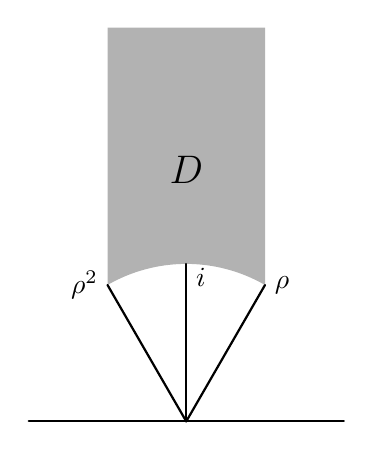
\begin{tikzpicture}[scale=2, line cap=round, line join=round]
        % 1. 定义基本参数
        % 这里的几何关系基于单位圆: rho = e^{i*pi/3}, rho^2 = e^{i*2pi/3}
        % 点的坐标: rho = (0.5, sqrt(3)/2), rho^2 = (-0.5, sqrt(3)/2)
        \def\sqthree{1.732/2} % sqrt(3)/2 约等于 0.866
        
        % 2. 绘制灰色阴影区域 D
        % 区域边界: 左垂直线 x=-0.5, 右垂直线 x=0.5, 下边界是单位圆弧
        \fill[gray!60] (-0.5, 2.5) -- (-0.5, \sqthree) 
            arc (120:60:1) -- (0.5, 2.5) -- cycle;

        % 3. 绘制辅助直线
        % 底部水平线 (实轴)
        \draw[thick] (-1, 0) -- (1, 0);
        
        % 从原点出发的三条射线
        \draw[thick] (0,0) -- (-0.5, \sqthree) coordinate (rho2);
        \draw[thick] (0,0) -- (0, 1) coordinate (i_point);
        \draw[thick] (0,0) -- (0.5, \sqthree) coordinate (rho);

        % 4. 绘制阴影区域的边界线（只画下方弧线, 两侧通常在示意图中由阴影界定）
        % 如果需要强化边界, 可以取消下面这行的注释: 
        % \draw[thick] (-0.5, 2.5) -- (-0.5, \sqthree) arc (120:60:1) -- (0.5, 2.5);

        % 5. 添加标签
        % D 标签在区域中心
        \node at (0, 1.6) {\Large $D$};
        
        % rho^2 标签（左侧）
        \node[left] at (rho2) {$\rho^2$};
        
        % rho 标签（右侧）
        \node[right] at (rho) {$\rho$};
        
        % i 标签（垂直线与圆弧交点处）
        % 原图中 i 放在交点右侧
        \node[below right, yshift=2pt] at (0, 1) {$i$};

    \end{tikzpicture}
    \]
\end{minipage}
\end{proposition}

\begin{proof}
定义 $G$ 为由 $S$ 和 $T$ 生成的 $\PSL_2(\mathbb{Z})$ 的子群 $\langle S, T \rangle$, 并设 $z \in \mathbb{H}$. 我们将证明存在一个 $g \in G$ 使得 $gz \in \bar{D}$. 若 $g = \begin{pmatrix} a & b \\ c & d \end{pmatrix} \in G$, 则
\[ \Im(gz) = \frac{\Im(z)}{|cz + d|^2} \]
对于任何 $N$, 满足 $|cz + d| < N$ 的整数对 $c, d \in \mathbb{Z}$ 只有有限多个, 因此可以选择 $g$ 使得 $|cz + d|$ 最小; 此时 $\Im(gz)$ 最大. 接下来我们选择 $n$ 使得
\[ -\frac{1}{2} \le \Re(T^n gz) \le \frac{1}{2}. \]
那么 $T^n gz \in \bar{D}$, 否则 $|T^n gz| < 1$, 并且
\[ \Im(ST^n gz) = \frac{\Im(T^n gz)}{|T^n gz|^2} > \Im(T^n gz) = \Im(gz), \]
这与 $g$ 的选择相矛盾. 我们已经证明了 $G \cdot \bar{D} = \mathbb{H}$; 特别地, $\PSL_2(\mathbb{Z}) \cdot \bar{D} = \mathbb{H}$. 

(b) 的证明以及 (a) 的其余部分是常规的 \cite[VII, 1.2]{serre1973}. 

对于 (c), 设 $h \in \PSL_2(\mathbb{Z})$, 并在 $D$ 中选择一个点 $z_0$. 存在 $G$ 中的元素 $g$ 使得 $ghz_0 \in \bar{D}$. 由于 $ghz_0$ 和 $z_0$ 处于同一个 $\PSL_2(\mathbb{Z})$ 轨道上, 根据 (a) 可知它们相等, 于是 (b) 表明 $gh = 1$. 因此 $h \in G$. 
\end{proof}

\begin{remark} \label{thm:5.1.4} 
\begin{enumerate}[label=\textup{(\alph*)}]
\item 可以证明模群 $\PSL_2(\mathbb{Z})$ 具有群展示(group presentation) $\langle S, T \mid S^2, (ST)^3 \rangle$. 换句话说, 它是 2 阶群 $\langle S \rangle$ 与 3 阶群 $\langle ST \rangle$ 的自由积. 许多有趣的有限群（例如, 除了四个之外的所有散在有限单群）都是由一个 2 阶元素和一个 3 阶元素生成的, 因此它们是 $\PSL_2(\mathbb{Z})$ 的商群. 
\item 设 $\Gamma$ 是 $\SL_2(\mathbb{Z})$ 的一个有限指数子群, 并记
\[ \SL_2(\mathbb{Z}) = \Gamma \gamma_1 \cup \dots \cup \Gamma \gamma_m \quad (\text{不交并}). \]
那么 $D' = \bigcup \gamma_i D$ 满足作为 $\Gamma$ 基本域的条件, 除了它可能不是连通的. 然而, 我们可以选取 $\gamma_i$ 使得 $D'$ 的闭包是连通的, 在这种情况下, 闭包的内部将成为 $\Gamma$ 的一个基本域. 
\end{enumerate}
\end{remark}

\subsection*{扩充上半平面}

$\SL_2(\mathbb{Z})$ 的元素通过射影线性变换作用于 $\mathbb{P}^1(\mathbb{C})$: 
\[ \begin{pmatrix} a & b \\ c & d \end{pmatrix} (z_1 : z_2) = (az_1 + bz_2 : cz_1 + \dd z_2). \]
我们将 $\mathbb{H}$、$\mathbb{Q}$ 和 $\{\infty\}$ 识别为 $\mathbb{P}^1(\mathbb{C})$ 的子集, 对应关系如下: 
\begin{align*}
    z &\leftrightarrow (z : 1) \quad z \in \mathbb{H} \\
    r &\leftrightarrow (r : 1) \quad r \in \mathbb{Q} \\
    \infty &\leftrightarrow (1 : 0).
\end{align*}

$\SL_2(\mathbb{Z})$ 在 $\mathbb{P}^1(\mathbb{C})$ 上的作用稳定了 $\mathbb{H}^* \stackrel{\text{def}}{=} \mathbb{H} \cup \mathbb{Q} \cup \{\infty\}$. 事实上: 
\begin{itemize}
    \item 若 $z \in \mathbb{H}$, 则 $\begin{pmatrix} a & b \\ c & d \end{pmatrix} (z : 1) = (az + b : cz + d) = \left( \frac{az+b}{cz+d} : 1 \right)$, 
    \item 若 $r \in \mathbb{Q}$, 则 $\begin{pmatrix} a & b \\ c & d \end{pmatrix} (r : 1) = (ar + b : cr + d) = 
    \begin{cases} 
        \left( \frac{ar+b}{cr+d} : 1 \right) & r \neq -\frac{d}{c} \\
        \infty & r = -\frac{d}{c},
    \end{cases}$
    \item $\begin{pmatrix} a & b \\ c & d \end{pmatrix} \infty = (a : c) = 
    \begin{cases} 
        \left( \frac{a}{c} : 1 \right) & c \neq 0 \\
        \infty & c = 0.
    \end{cases}$
\end{itemize}

在从 $\mathbb{H}$ 转换到 $\mathbb{H}^*$ 的过程中, 我们增加了一个额外的 $\SL_2(\mathbb{Z})$ 轨道. $\mathbb{H}^*$ 中不在 $\mathbb{H}$ 内的点被称为\emph{尖点 (cusps)}. 

\subsection*{$\mathbb{H}^*$ 上的拓扑}

我们按照以下方式赋予 $\mathbb{H}^*$ 拓扑: $\mathbb{H}$ 上的拓扑继承自 $\mathbb{C}$; 
集合
\[ \{z \mid \Im(z) > M\}, \quad M > 0 \]
构成了 $\infty$ 的一个基本邻域系; 集合
\[ \{z \mid |z - (a + ir)| < r\} \cup \{a\} \]
构成了 $a \in \mathbb{Q}$ 的一个基本邻域系. 可以证明 $\mathbb{H}^*$ 是Hausdorff空间, 且 $\SL_2(\mathbb{Z})$ 的作用是连续的. 

% TikZ 图表
\begin{center}
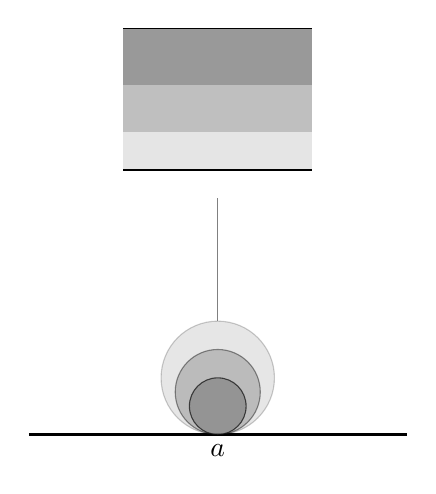
\begin{tikzpicture}[scale=1.2]
    % 绘制实轴
    \draw[thick] (-2,0) -- (2,0);
    \node[below] at (0,0) {$a$};

    % 绘制 a 处的邻域（圆/Horoballs）
    \foreach \r in {0.6, 0.45, 0.3} {
        \filldraw[fill=gray, opacity={1.1-\r*1.5}] (0,\r) circle (\r);
    }

    % 垂直连接线
    \draw[thin, gray] (0, 1.2) -- (0, 2.5);

    % 绘制无穷远处的邻域（水平带）
    \fill[gray!80] (-1, 3.7) rectangle (1, 4.3);
    \fill[gray!50] (-1, 3.2) rectangle (1, 3.7);
    \fill[gray!20] (-1, 2.8) rectangle (1, 3.2);
    \draw (-1, 2.8) -- (1, 2.8);
    \draw (-1, 4.3) -- (1, 4.3);

\end{tikzpicture}
\end{center}

\subsection*{$\Gamma \backslash \mathbb{H}^*$ 上的拓扑}

回想一下, 如果 $\pi: X \to Y$ 是一个满射且 $X$ 是拓扑空间, 那么 $Y$ 上的商拓扑定义为: 集合 $U$ 是开集当且仅当 $\pi^{-1}(U)$ 是开集. 通常情况下, 豪斯多夫空间在群作用下的商空间不一定是豪斯多夫空间, 即使轨道是闭的——这需要不同的轨道具有不交的开邻域. 

设 $\Gamma$ 是 $\SL_2(\mathbb{Z})$ 的有限指数子群. 离散群 $\Gamma$ 连续作用于 $\mathbb{H}$, 并且可以证明该作用是固有的\footnote{因此, 可以说 $\Gamma$ 在 $\mathbb{H}$ 上连续且固有地作用. 但在文献中, 通常称 $\Gamma$ 作用是“固有不连续的 (properly discontinuously)”. 参见 Lee 2003, p. 225 关于此术语的讨论. }. 即, 对于 $\mathbb{H}$ 中的任意一对点 $x, y$, 存在 $x$ 的邻域 $U$ 和 $y$ 的邻域 $V$ 使得集合
\[ \{ \gamma \in \Gamma \mid \gamma U \cap V \neq \emptyset \} \]
是有限的. 特别地, 这意味着 $\mathbb{H}$ 中每个点的稳定子群 (stabilizer) 都是有限的（这点我们已经知道了）. 


\begin{proposition} \label{thm:5.1.5}
\begin{enumerate}[label=\textup{(\alph*)}]
\item 对 $\mathbb{H}$ 的所有紧集 $A$ 与 $B$, $\{\gamma\in\Gamma \mid \gamma A\cap B\neq\varnothing\}$ 有限.
\item 每个 $z\in\mathbb{H}$ 有邻域 $U$ 使对 $\gamma\in\Gamma$, $\gamma U$ 与 $U$ 不相交, 除非 $\gamma z = z$.
\item 对 $\mathbb{H}$ 中不在同一 $\Gamma$-轨道中的点 $x, y$, 存在 $x$ 的邻域 $U$ 与 $y$ 的邻域 $V$ 使对所有 $\gamma\in\Gamma$ 有 $\gamma U\cap V = \varnothing$.
\end{enumerate}
\end{proposition}

\begin{proof}
\begin{enumerate}[label=\textup{(\alph*)}]
\item 由 $\Gamma$ 连续且真作用容易推出.

\item 设 $V$ 为 $z$ 的紧邻域, $S$ 为使 $V\cap\gamma V\neq\varnothing$ 但 $\gamma$ 不固定 $z$ 的 $\gamma\in\Gamma$ 的集合. 由 (a), $S$ 有限. 对每个 $\gamma\in S$, 选取 $z$ 的邻域 $V_\gamma$ 与 $\gamma z$ 的邻域 $W_\gamma$ 不相交, 令
\[
U = V\cap\bigcap_{\gamma\in S}(V_\gamma\cap\gamma^{-1}W_\gamma).
\]
对 $\gamma\in S$, $\gamma U\subset W_\gamma$. 因 $W_\gamma$ 与 $V_\gamma$ 不相交且 $V_\gamma$ 含 $U$, 这蕴含 $\gamma U$ 与 $U$ 不相交.

\item 选取 $x$ 的紧邻域 $A$ 与 $y$ 的紧邻域 $B$, 令 $S$ 为使 $\gamma A\cap B\neq\varnothing$ 的 (有限) $\gamma$ 集. 因 $\gamma x\neq y$, 对每个 $\gamma\in S$ 存在 $\gamma x$ 与 $y$ 的不相交邻域 $U_\gamma$ 与 $V_\gamma$. 则 $U = A\cap\bigcap_{\gamma\in S}\gamma^{-1}U_\gamma$ 与 $V = B\cap\bigcap_{\gamma\in S}V_\gamma$ 分别是 $x$ 与 $y$ 的邻域, 使对所有 $\gamma\in\Gamma$, $\gamma U$ 与 $V$ 不相交.
\end{enumerate}
\end{proof}

\begin{corollary} \label{thm:5.1.6}
空间 $\Gamma\setminus\mathbb{H}$ 是 Hausdorff 的.
\end{corollary}

\begin{proof}
设 $x$ 与 $y$ 是 $\mathbb{H}$ 中不在同一 $\Gamma$-轨道中的点, 按上一命题的 (c) 选取 $x$ 与 $y$ 的邻域 $U$ 与 $V$. 则 $\Gamma U$ 与 $\Gamma V$ 是 $\Gamma x$ 与 $\Gamma y$ 的不相交邻域.
\end{proof}

\begin{proposition} \label{thm:5.1.7}
空间 $\Gamma\setminus\mathbb{H}^*$ 是 Hausdorff 的且紧致.
\end{proposition}

\begin{proof}
由推论 \ref{thm:5.1.6}, 为证 $\Gamma\setminus\mathbb{H}^*$ Hausdorff, 只剩检验尖点附近, 留给读者 (见下一小节). 空间 $\Gamma\setminus\mathbb{H}^*$ 是 $\SL_2(\mathbb{Z})\setminus\mathbb{H}^*$ 的商, 后者紧致, 因 $\bar{D}\cup\{\infty\}$ 紧致.
\end{proof}

\subsection*{$\Gamma_0(N)\setminus\mathbb{H}^*$ 上的复结构}

我们将特别感兴趣的 $\SL_2(\mathbb{Z})$ 的子群是 Hecke 子群\index{Hecke@Hecke 子群(Hecke subgroups)}
\[
\Gamma_0(N) = \left\{\begin{pmatrix}a & b\\ c & d\end{pmatrix}\;\Big|\; c\equiv 0\pmod{N}\right\}.
\]
记 $\Gamma_0(1) = \SL_2(\mathbb{Z})$. 整数 $N$ 称为 $\Gamma_0(N)$ 的级 (level)\index{ji@级(level)}.

现在定义 $\Gamma_0(N)\setminus\mathbb{H}^*$ 上的复结构. 对 $z_0\in\mathbb{H}$, 选取 $z_0$ 的邻域 $V$ 使
\[
\gamma V\cap V\neq\varnothing\Rightarrow\gamma z_0 = z_0,
\]
令 $U = \pi(V)$——它开, 因 $\pi^{-1}U = \bigcup\gamma V$ 开.

若 $z_0$ 在 $\Gamma_0(N)$ 中的稳定子是 $\pm I$, 则 $\pi\colon V\to U$ 是同胚, 以 $\varphi$ 记其逆, 要求 $(U, \varphi)$ 是坐标邻域.

若 $z_0$ 在 $\Gamma_0(N)$ 中的稳定子 $\neq\{\pm I\}$, 则它是 $2m$ 阶循环群且 $m = 2$ 或 $3$ (它在 $\Gamma_0(N)/\{\pm I\}$ 中的像阶为 $2$ 或 $3$)——见 \ref{thm:5.1.3}b. 分式线性变换
\[
\lambda\colon\mathbb{H}\to D, \quad z\mapsto\frac{z - z_0}{z - \bar{z}_0},
\]
把 $z_0$ 送到单位圆盘 $D$ 中的 $0$. 存在良定义的映射 $\varphi\colon U\to\mathbb{C}$ 使 $\varphi(\pi(z)) = \lambda(z)^m$, 要求 $(U, \varphi)$ 是坐标邻域 (参看例 \ref{thm:5.1.2}).

再考虑 $z_0 = \infty$. 选取 $V$ 为 $\infty$ 的邻域 $\{z\mid \Im(z) > 2\}$, 令 $U = \pi(V)$. 若
\[
z\in V\cap\gamma V, \quad \gamma = \begin{pmatrix}a & b\\ c & d\end{pmatrix}\in\Gamma_0(N),
\]
则
\[
2\le\Im(\gamma z) = \frac{\Im(z)}{|cz + d|^2}\le\frac{1}{|c|^2\Im(z)}\le\frac{1}{2|c|^2}
\]
故 $c = 0$. 因此
\[
\gamma = \pm\begin{pmatrix}1 & m\\ 0 & 1\end{pmatrix},
\]
故存在良定义的映射 $\varphi\colon U\to\mathbb{C}$ 使 $\varphi(\pi(z)) = e^{2\pi iz}$, 要求 $(U, \varphi)$ 是坐标邻域 (参看例 \ref{thm:5.1.1}).

对 $z_0\in\mathbb{Q}$, 选取 $\beta\in\SL_2(\mathbb{Z})$ 使 $\beta(z_0) = \infty$, 类似处理.

\begin{proposition} \label{thm:5.1.8}
上面定义的坐标邻域相容, 故在 $\Gamma_0(N)\setminus\mathbb{H}^*$ 上定义 Riemann 曲面结构.
\end{proposition}

\begin{proof}
常规练习.
\end{proof}

把 Riemann 曲面 $\Gamma_0(N)\setminus\mathbb{H}^*$ 记为 $X_0(N)$, 其开子曲面 $\Gamma_0(N)\setminus\mathbb{H}$ 记为 $Y_0(N)$.

\subsection*{$X_0(N)$ 的亏格}

Riemann 曲面的亏格可通过``三角剖分''并使用公式
\[
2 - 2g = V - E + F
\]
计算, 其中 $V$ 是顶点数, $E$ 是边数, $F$ 是面数. 例如, 球面可从正四面体投影出去来三角剖分, 此时 $V = 4$, $E = 6$, $F = 4$, 故如愿 $g = 0$.

\begin{proposition} \label{thm:5.1.9}
Riemann 曲面 $X_0(1)$ 亏格为零.
\end{proposition}

\begin{proof}
取赤道上三点及上下半球为面, 得球面的一个``假''三角剖分, 它给出正确的亏格 $2 = 3 - 3 + 2$, 但违反三角剖分的通常定义 (要求任两个三角形交于单边、单点或不交). 加上北极点为顶点并与赤道三顶点相连, 可变成合法三角剖分.

取三个顶点 $\rho$, $i$ 与 $\infty$ 及连接它们的显然曲线 ($D$ 的边界上两条及从 $i$ 到 $\infty$ 的虚轴一条), 得 $X_0(1)$ 的一个假三角剖分. 在 $D$ 中实部 $> 0$ 处加上第四点并与 $\rho$, $i$, $\infty$ 相连, 可变成合法三角剖分.
\end{proof}

对紧 Riemann 曲面的有限映射 $\pi\colon Y\to X$, Riemann--Hurwitz 公式把 $Y$ 的亏格 $g_Y$ 与 $X$ 的亏格 $g_X$ 联系起来:
\[
2g_Y - 2 = (2g_X - 2)m + \sum_{Q\in Y}(e_Q - 1).
\]
这里 $m$ 是映射的次数, 故除有限多个 $P$ 外 $\pi^{-1}(P)$ 有 $m$ 个元素; $e_Q$ 是分歧指数, 故除至少两叶在 $\pi(Q)$ 之上相交于 $Q$ 外 $e_Q = 1$, 此时 $e_Q$ 是这种叶数.

例如, 若 $E$ 是椭圆曲线
\[
E\colon Y^2Z = X^3 + aXZ^2 + bZ^3, \quad a,b\in\mathbb{C}, \quad\Delta\neq 0,
\]
而 $\pi$ 是映射
\[
\infty\mapsto\infty, \quad (x:y:z)\mapsto(x:z)\colon E(\mathbb{C})\to\mathbb{P}^1(\mathbb{C}),
\]
则 $m = 2$ 且除 $Q = \infty$ 或 $E$ 的三个 $2$ 阶点之一外 $e_Q = 1$, 此时 $e_Q = 2$. 这与 $E(\mathbb{C})$ 亏格 $1$ 而 $\mathbb{P}^1(\mathbb{C})$ (Riemann 球面) 亏格 $0$ 相符.

Riemann--Hurwitz 公式的证明: 三角剖分 $Y$ 使分歧点为顶点且 $Y$ 的三角剖分位于 $X$ 的三角剖分之上.

现在可通过研究商映射 $X_0(N)\to X_0(1)$ 来计算 $X_0(N)$ 的亏格. 仅有的 (可能) 分歧点是 $\Gamma_0(1)$-等价于 $i$, $\rho$ 或 $\infty$ 的点. 显式公式见 \cite[pp.~23--25]{shimura1971}. 例如, 对素数 $p > 3$,
\[
\operatorname{genus}(X_0(p)) = \begin{cases} n - 1 & \text{若 } p = 12n + 1,\\ n & \text{若 } p = 12n + 5, 12n + 7,\\ n + 1 & \text{若 } p = 12n + 11.\end{cases}
\]
此外,
\begin{gather*}
g = 0 \text{ 若 } N = 1, 2, 3, \dots, 10, 12, 13, 16, 18, 25,\\
g = 1 \text{ 若 } N = 11, 14, 15, 17, 19, 20, 21, 24, 27, 32, 36, 49,\\
g = 2 \text{ 若 } N = 22, 23, 26, 28, 29, 31, 37, 50.
\end{gather*}

\begin{exercise} \label{thm:5.1.10}
对素数 $p$, 证明 $\Gamma_0(p)$ 在 $\mathbb{P}^1(\mathbb{Q})$ 上的自然作用只有两个轨道, 以 $0$ 与 $\infty = (1:0)$ 为代表. 推出 $X_0(p)\setminus Y_0(p)$ 恰有两个元素.
\end{exercise}


\section{\texorpdfstring{$X_0(N)$ 作为 $\mathbb{Q}$ 上的代数曲线}{X0(N) 作为 Q 上的代数曲线}}\label{sec:5.2}

上一节定义了紧 Riemann 曲面 $X_0(N)$. 一般定理说每个紧 Riemann 曲面 $X$ 可等同于 $\mathbb{C}$ 上唯一的非奇异射影代数曲线 $C$ 的复点集. 但一般地 $C$ 不能定义在 $\mathbb{Q}$ 上 (甚至 $\mathbb{Q}^{\mathrm{al}}$ 上)——例如考虑\hyperref[ch:3]{第三章}中 $j$-不变量超越的 Riemann 曲面 $\mathbb{C}/\Lambda$——且当 $C$ 能定义在 $\mathbb{Q}$ 上时, 一般地它不能以任何典范方式定义——考虑 $j(E)\in\mathbb{Q}$ 的 $\mathbb{C}$ 上椭圆曲线 $E$.

本节将看到 $X_0(N)$ 有非凡性质: 它是 $\mathbb{Q}$ 上典范曲线的复点集.

\subsection*{模函数\index{hanshu@函数(function)!mo@模(modular)}}

对连通紧 Riemann 曲面 $X$, $X$ 上的亚纯函数构成 $\mathbb{C}$ 上超越次数 $1$ 的域. 我们确定 $X = X_0(N)$ 的此域.

对 $\SL_2(\mathbb{Z})$ 中有限指数的子群 $\Gamma$, $\Gamma\setminus\mathbb{H}^*$ 上的亚纯函数称为 $\Gamma$ 的模函数 (modular functions). 若 $\pi\colon\mathbb{H}\to\Gamma\setminus\mathbb{H}^*$ 是商映射, 则 $g\mapsto\pi\circ g$ 把 $\Gamma$ 的模函数等同于满足下列条件的 $\mathbb{H}$ 上的函数 $f$:
\begin{enumerate}[label=\textup{(\alph*)}]
\item $f$ 在 $\mathbb{H}$ 上亚纯;
\item 对所有 $\gamma\in\Gamma$, $f(\gamma z) = f(z)$;
\item $f$ 在尖点 (即 $\mathbb{H}^*\setminus\mathbb{H}$ 的点) 处亚纯.
\end{enumerate}

\subsection*{$X_0(1)$ 上的亚纯函数}

设 $S$ 为 Riemann 球面 $S = \mathbb{C}\cup\{\infty\}$ (III\ref{thm:3.3.2}). $S$ 上的亚纯函数是 $z$ 的有理函数, $S$ 的自同构是分式线性变换
\[
z\mapsto\frac{az+b}{cz+d}, \qquad a, b, c, d\in\mathbb{C}, \ ad-bc\neq 0.
\]
{\emergencystretch=3em 事实上 $\operatorname{Aut}(S) = \mathrm{PGL}_2(\mathbb{C}) \overset{\text{def}}{=} \GL_2(\mathbb{C})/\mathbb{C}^{\times}$. 且给定 $S$ 上两组不同点集 $\{P_1, P_2, P_3\}$ 与 $\{Q_1, Q_2, Q_3\}$, 存在唯一的分式线性变换把每个 $P_i$ 送到 $Q_i$. (最后陈述的证明是线性代数的容易的练习: 给定 $\mathbb{C}^2$ 中两组不同直线 $\{L_1, L_2, L_3\}$ 与 $\{M_1, M_2, M_3\}$, 存在把每个 $L_i$ 送到 $M_i$ 的线性变换, 且该线性变换在相差非零常数乘法的意义下唯一.)\par}

回忆 $1, i$ 与 $\rho$ 是 $\mathbb{H}^*$ 中的点. 用相同符号记它们在 $X_0(1)$ 中的像.

\begin{proposition} \label{thm:5.2.1} 
存在 $X_0(1)$ 上唯一的亚纯函数 $J$, 除在 $\infty$ 处有单极点外全纯, 且取值
\[
J(i) = 1, \qquad J(\rho) = 0.
\]
$X_0(1)$ 上的亚纯函数是 $J$ 的有理函数.
\end{proposition}

\begin{proof}
由上一节, $X_0(1)$ 作为 Riemann 曲面同构于 Riemann 球面 $S$. 设 $f\colon X_0(1)\to S$ 为同构, $P, Q, R$ 为 $\rho, i, \infty$ 的像. 存在唯一的分式线性变换 $L$ 把 $P, Q, R$ 送到 $0, 1, \infty$, 而复合 $J = L\circ f$ 具有所需性质. 若 $J'$ 是第二个具有所需性质的函数, 则复合 $J'\circ J^{-1}$ 是固定 $0, 1, \infty$ 的 $S$ 的自同构, 故是恒等映射. 对第二个陈述, 注意 $J$ 定义 $X_0(1)$ 到 Riemann 球面的同构, 在此下 Riemann 球面上的亚纯函数 $z$ 对应 $X_0(1)$ 上的 $J$.
\end{proof}

我们希望识别函数 $J$. 回忆\hyperref[ch:3]{第三章}, 对 $\mathbb{C}$ 中的格 $\Lambda$, $G_{2k}(\Lambda) \overset{\text{def}}{=} \sum_{\omega\in\Lambda, \omega\neq 0}\frac{1}{\omega^{2k}}$, 且 $G_{2k}(z) \overset{\text{def}}{=} G_{2k}(\mathbb{Z}z + \mathbb{Z})$, $z\in\mathbb{H}$. 且 (III\ref{thm:3.2.6}) 映射 $z\mapsto(\wp(z):\wp'(z):1)$ 是从 $\mathbb{C}/\mathbb{Z}z + \mathbb{Z}$ 到椭圆曲线
\[
Y^2Z = 4X^3 - g_4(z)XZ^2 - g_6(z)Z^3, \qquad \Delta = g_4(z)^3 - 27g_6(z)^2\neq 0
\]
的同构, 其中 $g_4(z) = 60G_4(z)$, $g_6(z) = 140G_6(z)$. 此曲线的 $j$-不变量是
\[
j(z) = \frac{1728g_4(z)^3}{\Delta}.
\]
由定义显然 $G_{2k}(z)$, $\Delta(z)$ 与 $j(z)$ 在 $T\colon z\mapsto z+1$ 下不变, 故可用变量 $q = e^{2\pi iz}$ 表示. 在 \cite[VII, 方程 (23, 33, 42)]{serre1973} 中, 可找到以下展开:
\begin{align}
G_{2k}(z) &= 2\zeta(2k) + \frac{2(2\pi i)^{2k}}{(2k-1)!}\sum_{n=1}^{\infty}\sigma_{2k-1}(n)q^n, \qquad \sigma_k(n) = \sum_{d\mid n}d^k, \tag{42} \label{eq:42} \\
\Delta &= (2\pi)^{12}(q - 24q^2 + 252q^3 - 1472q^4 + \cdots), \tag{43} \label{eq:43} \\
j &= \frac{1}{q} + 744 + 196884q + 21493760q^2 + \sum_{n\ge 3}c(n)q^n, \qquad c(n)\in\mathbb{Z}. \tag{44} \label{eq:44}
\end{align}
$G_{2k}(z)$ 公式的证明初等, 其余由它与 $\zeta(2k)$ 的初等结果推出. 传统上在 $j$ 的公式中包含因子 $1728$, 使它在无穷远处留数为 $1$.

函数 $j$ 在 $\Gamma_0(1) = \SL_2(\mathbb{Z})$ 下不变, 因为 $j(z)$ 只依赖格 $\mathbb{Z}z + \mathbb{Z}$. 且:
\begin{itemize}
\item $j(\rho) = 0$, 因为 $\mathbb{C}/\mathbb{Z}\rho + \mathbb{Z}$ 有 $\rho^2 = \sqrt[3]{1}$ 的复乘法, 故形如 $Y^2 = X^3 + b$, 其 $j$-不变量为 $0$;
\item $j(i) = 1728$, 因为 $\mathbb{C}/\mathbb{Z}i + \mathbb{Z}$ 有 $i$ 的复乘法, 故形如 $Y^2 = X^3 + aX$.
\end{itemize}
故 $j = 1728J$, 可把命题 \ref{thm:5.2.1} 重述如下.

\begin{proposition} \label{thm:5.2.2} 
函数 $j$ 是 $X_0(1)$ 上除在 $\infty$ 处有单极点外全纯、且取值
\[
j(i) = 1728, \qquad j(\rho) = 0
\]
的唯一亚纯函数. 它定义从 $X_0(1)$ 到 Riemann 球面的同构, 故 $X_0(N)$ 上的亚纯函数域是 $\mathbb{C}(j)$.
\end{proposition}

\subsection*{$X_0(N)$ 上的亚纯函数}

定义 $j_N$ 为 $\mathbb{H}$ 上满足 $j_N(z) = j(Nz)$ 的函数. 对 $\gamma\in\Gamma_0(1)$, 人们想写
\[
j_N(\gamma z) \overset{\text{def}}{=} j(N\gamma z) = j(\gamma Nz) = j(Nz) \overset{\text{def}}{=} j_N(z),
\]
但一般地, 这是不对的, 因为 $N\gamma z\neq\gamma Nz$. 不过, 若 $\gamma\in\Gamma_0(N)$, 则 $j_N(\gamma z) = j_N(z)$ 为真. 为看到这点, 设 $\gamma = \begin{pmatrix}a & b\\ c & d\end{pmatrix}\in\Gamma_0(N)$, 故 $c = Nc'$, $c'\in\mathbb{Z}$. 则
\[
j_N(\gamma z) = j\left(\frac{Naz + Nb}{cz + d}\right) = j\left(\frac{a(Nz) + Nb}{c'(Nz) + d}\right) = j(\gamma' Nz),
\]
其中 $\gamma' = \begin{pmatrix}a & Nb\\ c' & b\end{pmatrix}\in\Gamma_0(1)$, 故 $j(\gamma' Nz) = j(Nz) = j_N(z)$. 因此 $j_N$ 在 $\Gamma_0(N)$ 下不变, 故定义 $X_0(N)$ 上的亚纯函数.

\begin{theorem} \label{thm:5.2.3} 
$X_0(N)$ 上的亚纯函数域是 $\mathbb{C}(j, j_N)$.
\end{theorem}

\begin{proof}
曲线 $X_0(N)$ 是 $X_0(1)$ 的度数 $m$ 等于 $(\Gamma_0(1):\Gamma_0(N))$ 的覆盖. 一般理论蕴含 $X_0(N)$ 上亚纯函数域在 $\mathbb{C}(j)$ 上的次数为 $m$, 但我们再证一遍. 设 $\{\gamma_1 = 1, \dots, \gamma_m\}$ 为 $\Gamma_0(N)$ 在 $\Gamma_0(1)$ 中右陪集的代表元集, 故
\[
\Gamma_0(1) = \bigsqcup_{i=1}^{m}\Gamma_0(N)\gamma_i
\]
(无交并). $\Gamma_0(1)$ 中元素 $\gamma$ 的右乘置换陪集 $\Gamma_0(N)\gamma_i$, 故 $\{\gamma_1, \dots, \gamma_m\}$ 也是 $\Gamma_0(N)$ 在 $\Gamma_0(1)$ 中右陪集的代表元集.

若 $f(z)$ 是 $\Gamma_0(N)$ 的模函数, 则 $f(\gamma_i z)$ 只依赖陪集 $\Gamma_0(N)\gamma_i$. 故函数 $\{f(\gamma_i' z)\}$ 是函数 $\{f(\gamma_i z)\}$ 的置换, 且 $f(\gamma_i z)$ 的每个对称多项式在 $\Gamma_0(1)$ 下不变; 因这样的多项式显然满足其他条件, 它是 $\Gamma_0(1)$ 的模函数, 从而是 $j$ 的有理函数. 故 $f(z)$ 满足系数在 $\mathbb{C}(j)$ 中、次数 $m$ 的多项式, 即 $\prod(Y - f(\gamma_i z))$. 因这对 $X_0(N)$ 上每个亚纯函数成立, 我们看到此类函数的域在 $\mathbb{C}(j)$ 上的次数至多为 $m$ (应用本原元素定理, \cite[5.1]{milne-ft}).

接着我断言所有 $f(\gamma_i z)$ 都在 $\mathbb{C}(j)$ 上与 $f(z)$ 共轭: 设 $F(j, Y)$ 为 $f(z)$ 在 $\mathbb{C}(j)$ 上的最小多项式, 故把 $F(j, Y)$ 视为 $Y$ 的系数在 $\mathbb{C}(j)$ 中的多项式时首一且不可约; 把 $z$ 换成 $\gamma_i z$ 并记得 $j(\gamma_i z) = j(z)$, 得 $F(j(z), f(\gamma_i z)) = 0$, 这证明断言.

若能证明函数 $j(N\gamma_i z)$ 互不相同, 则 $j_N$ 在 $\mathbb{C}(j)$ 上的最小多项式次数为 $m$, 且 $X_0(N)$ 上亚纯函数域在 $\mathbb{C}(j)$ 上的次数为 $m$, 由 $j_N$ 生成.

设对某些 $i\neq j$, $j(N\gamma_i z) = j(N\gamma_j z)$. 回忆 (\ref{thm:5.2.2}) $j$ 定义同构 $\Gamma_0(1)\setminus\mathbb{H}^*\to S$ (Riemann 球面), 故
\[
j(N\gamma_i z) = j(N\gamma_j z) \ \forall z \implies \exists\gamma\in\Gamma_0(1) \text{ 使 } N\gamma_i z = \gamma N\gamma_j z \ \forall z,
\]
这蕴含
\[
\begin{pmatrix}N & 0\\ 0 & 1\end{pmatrix}\gamma_i = \pm\gamma\begin{pmatrix}N & 0\\ 0 & 1\end{pmatrix}\gamma_j.
\]
故
\[
\gamma_i\gamma_j^{-1}\in\Gamma_0(1)\cap\begin{pmatrix}N & 0\\ 0 & 1\end{pmatrix}^{-1}\Gamma_0(1)\begin{pmatrix}N & 0\\ 0 & 1\end{pmatrix} = \Gamma_0(N),
\]
这与 $\gamma_i$ 与 $\gamma_j$ 在不同陪集中矛盾.
\end{proof}

由证明, $j_N$ 在 $\mathbb{C}(j)$ 上的最小多项式是
\[
F_N(j, Y) = \prod_{i=1}^{m}(Y - j(N\gamma_i z)).
\]
{\emergencystretch=3em $j(N\gamma_i z)$ 的对称多项式在 $\mathbb{H}$ 上全纯. 因它们是有理函数 $j(z)$, 它们必是 $j(z)$ 的多项式, 故 $F_N(j, Y)\in\mathbb{C}[j, Y]$ (而非 $\mathbb{C}(j)[Y]$).\par}

把 $j$ 换成变量 $X$, 得多项式 $F_N(X, Y)\in\mathbb{C}[X, Y]$,
\[
F_N(X, Y) = \sum c_{r,s}X^rY^s, \qquad c_{r,s}\in\mathbb{C}, \ c_{0,m} = 1.
\]
我断言 $F_N(X, Y)$ 是满足 $c_{0,m} = 1$ 的 $Y$ 的次数 $\le m$ 的唯一多项式, 使 $F_N(j, j_N) = 0$. 事实上, $F_N(X, Y)$ 生成 $\mathbb{C}[X, Y]$ 中满足 $G(j, j_N) = 0$ 的一切多项式 $G(X, Y)$ 的理想, 由此推出断言.

\begin{proposition} \label{thm:5.2.4} 
多项式 $F_N(X, Y)$ 的系数在 $\mathbb{Q}$ 中.
\end{proposition}

\begin{proof}
我们知道
\[
j(z) = q^{-1} + \sum_{n\ge 0}c(n)q^n, \qquad c(n)\in\mathbb{Z}.
\]
把它代入方程 $F_N(j(z), j(Nz)) = 0$, 令 $q$ 的幂的系数相等, 得到系数在 $\mathbb{Q}$ 中、未知数 $c_{r,s}$ 的线性方程组, 而附加方程 $c_{0,m} = 1$ 后, 该系统唯一决定 $c_{r,s}$. 因线性方程组在 $\mathbb{C}$ 中有解, 它在 $\mathbb{Q}$ 中也有解 (看矩阵的秩); 因解唯一, $\mathbb{C}$ 中的解必在 $\mathbb{Q}$ 中. 故 $c_{r,s}\in\mathbb{Q}$.
\end{proof}

\begin{aside} \label{thm:5.2.5} 
多项式 $F_N(X, Y)$ 由 Kronecker 在 100 多年前引入. 已知它有整数系数且在 $X$ 与 $Y$ 中对称. 对 $N = 2$, 它是
\begin{align*}
  X^3 + Y^3 - X^2Y^2 + 1488XY(X+Y) - 162000(X^2+Y^2)\\
  + 40773375XY + 8748000000(X+Y) - 157464000000000.
\end{align*}
对 $N = 2, 3, 5, 7$ 分别由 Smith (1878, 1879), Berwick (1916) 与 Herrmann (1974) 计算. 此时人类放弃了, 改用计算机, 1984 年找到 $F_{11}$. 这最后计算在 VAX-780 上用了约 20 小时, 结果是系数高达 $10^{60}$、写出来要五页的多项式. 此后计算 $F_N(X, Y)$ 的算法有改进, 且对至少到 $3{,}600$ 的一切素数 $\ell$ 计算了 $F_\ell(X, Y)$ (\cite{broker2012}). 对我们重要的是知道该多项式存在; 知道它是什么并不重要.
\end{aside}

\subsection*{$\mathbb{Q}$ 上的曲线 $X_0(N)$}

设 $C_N$ 为方程 $F_N(X, Y) = 0$ 的 $\mathbb{Q}$ 上仿射曲线, $\bar{C}_N$ 为由齐次化的 $F_N$ 定义的射影曲线. 映射 $z\mapsto(j(z), j(Nz))$ 是 $X_0(N)\setminus\Sigma\to C_N(\mathbb{C})$ 的映射, 其中 $\Sigma$ 是 $j$ 或 $j_N$ 有极点的集合. 该映射唯一延拓为 $X_0(N)\to\bar{C}_N(\mathbb{C})$ 的映射, 它在 $\bar{C}_N$ 的奇异点之外是同构, 而序对 $(X_0(N), X_0(N)\to\bar{C}_N(\mathbb{C}))$ 由 $\bar{C}_N$ 唯一确定 (在唯一同构的意义下): 它是 $\bar{C}_N$ 在 $\mathbb{C}$ 上的典范``消解'' (desingularization).\footnote{正则映射 $X_0(N)\setminus\Sigma\to C_N$ 在函数域上诱导同构, 它把 $X_0(N)$ 实现为 $\bar{C}_N$ 的规范化.}

现在考虑 $\mathbb{Q}$ 上的 $\bar{C}_N$. 存在 $\mathbb{Q}$ 上的典范消解 $X\to\bar{C}_N$, 即 $\mathbb{Q}$ 上射影非奇异曲线 $X$ 与正则映射 $X\to\bar{C}_N$, 它在 $\bar{C}_N$ 的奇异点之外是同构, 且序对 $(X, X\to\bar{C}_N)$ 由 $\bar{C}_N$ 唯一确定 (在唯一同构的意义下). 见 I, 定理~\ref{thm:1.6.4}. 过渡到 $\mathbb{C}$-点, 我们看到 $(X(\mathbb{C}), X(\mathbb{C})\to\bar{C}_N(\mathbb{C}))$ 具有刻画 $(X_0(N), X_0(N)\to\bar{C}_N(\mathbb{C}))$ 的性质, 故存在与到 $\bar{C}_N(\mathbb{C})$ 的映射相容的唯一 Riemann 曲面同构 $X_0(N)\to X(\mathbb{C})$.

总结: 有良定义的 $\mathbb{Q}$ 上曲线 $X$, $\mathbb{Q}$ 上正则映射 $\psi\colon X\to\bar{C}_N$, 与同构 $X_0(N)\to X(\mathbb{C})$, 其与 $\psi(\mathbb{C})$ 的复合 (在某个有限集之外) 是 $z\mapsto(j(z), j(Nz))$.

今后, 常用 $X_0(N)$ 表示 $\mathbb{Q}$ 上曲线 $X$——从上下文应清楚指 $\mathbb{Q}$ 上曲线还是 Riemann 曲面. 仿射曲线 $X_0(N)\setminus\{\text{尖点}\}\subset X_0(N)$ 记为 $Y_0(N)$; 故 $Y_0(N)(\mathbb{C}) = \Gamma_0(N)\setminus\mathbb{H}$.

\begin{remark} \label{thm:5.2.6} 
曲线 $F_N(X, Y) = 0$ 高度奇异, 因为若无奇点, 公式~\eqref{eq:6} 将预测过高的亏格.
\end{remark}

\subsection*{$X_0(N)$ 上的点}

由于不能写下 $X_0(N)$ 作为 $\mathbb{Q}$ 上非奇异射影曲线的方程, 我们至少想知道它在任何含 $\mathbb{Q}$ 的域中的点是什么. 这可以做到.

先看 $X_0(N)$ 的复点, 即 Riemann 曲面 $X_0(N)$. 此时有图
\[
\begin{tikzcd}[row sep=3em, column sep=3em]
    \{(E,S)\}/\approx \arrow[d] \arrow[r, leftrightarrow] & 
    \{(\Lambda,S)\}/\mathbb{C}^\times \arrow[d] \arrow[r, leftrightarrow] & 
    \Gamma_0(N)\backslash M/\mathbb{C}^\times \arrow[d] \arrow[r, leftrightarrow] & 
    \Gamma_0(N)\backslash \mathbb{H} \arrow[d] \\
    \{E\}/\approx \arrow[r, leftrightarrow] & 
    \mathcal{L}/\mathbb{C}^\times \arrow[r, leftrightarrow] & 
    \Gamma_0(1)\backslash M/\mathbb{C}^\times \arrow[r, leftrightarrow] & 
    \Gamma_0(1)\backslash \mathbb{H}
\end{tikzcd}
\]
其中各项现在解释. 所有符号 $\longleftrightarrow$ 都是自然双射. 底行合并了\hyperref[ch:3]{第三章}的映射.

回忆 $M$ 是满足 $\Im(\omega_1/\omega_2) > 0$ 的序对 $(\omega_1, \omega_2)\in\mathbb{C}\times\mathbb{C}$ 的集合 (故 $M/\mathbb{C}^{\times}\cong\mathbb{P}^1(\mathbb{C})$), 而双射 $M/\mathbb{C}^{\times}\to\mathbb{H}$ 把 $(\omega_1, \omega_2)$ 送到 $\omega_1/\omega_2$. 右方格其余部分现在显然.

回忆 $L$ 是 $\mathbb{C}$ 中格的集合, 且 $M$ 中两个序对定义的格相等当且仅当序对位于同一 $\Gamma_0(1)$-轨道中. 故从 $M$ 的元素过渡到其 $\Gamma_0(1)$-轨道时, 忘记基而只记住格. 从 $M$ 的元素过渡到其 $\Gamma_0(N)$-轨道时, 记下基的一点点, 因为设
\[
\begin{pmatrix}\omega_1'\\ \omega_2'\end{pmatrix} = \begin{pmatrix}a & b\\ c & d\end{pmatrix}\begin{pmatrix}\omega_1\\ \omega_2\end{pmatrix}, \qquad \begin{pmatrix}a & b\\ c & d\end{pmatrix}\in\Gamma_0(N).
\]
则 $\omega_1' = a\omega_1 + b\omega_2$, $\omega_2' = c\omega_1 + d\omega_2\equiv d\omega_2\pmod{N\Lambda}$. 故 $\frac{1}{N}\omega_2'\equiv\frac{d}{N}\omega_2\pmod{\Lambda}$. 注意因 $\begin{pmatrix}a & b\\ c & d\end{pmatrix}$ 行列式为 $1$, $\gcd(d, N) = 1$, 故 $\frac{1}{N}\omega_2'$ 与 $\frac{1}{N}\omega_2$ 在 $\mathbb{C}/\Lambda$ 中生成同一 $N$ 阶循环子群 $S$. 因此, 映射
\[
(\omega_1, \omega_2)\mapsto\left(\Lambda(\omega_1, \omega_2), \left\langle\frac{1}{N}\omega_2\right\rangle\right)
\]
定义从 $\Gamma_0(N)\setminus M$ 到由 $\mathbb{C}$ 中格 $\Lambda$ 与 $\mathbb{C}/\Lambda$ 中 $N$ 阶循环子群 $S$ 组成的序对之集的双射. 现在 $(\Lambda, S)\mapsto(\mathbb{C}/\Lambda, S)$ 定义最后这个集合与由 $\mathbb{C}$ 上椭圆曲线 $E$ 与 $E(\mathbb{C})$ 中 $N$ 阶循环子群 $S$ 组成的序对 $(E, S)$ 的同构类集之间的一一对应. 同构 $(E, S)\to(E', S')$ 是把 $S$ 送入 $S'$ 的同构 $E\to E'$.

注意 $E$ 对 $S$ 的商
\[
E/S\cong\mathbb{C}/\Lambda(\omega_1, \frac{1}{N}\omega_2),
\]
且 $\omega_1/(\frac{1}{N}\omega_2) = N\frac{\omega_1}{\omega_2}$. 故若 $j(E) = j(z)$, 则 $j(E/S) = j(Nz)$.

现在, 对任何域 $k\supset\mathbb{Q}$, 定义 $\mathcal{E}_0(N)(k)$ 为序对 $(E,S)$ 的同构类集, 其中 $E$ 是 $k$ 上椭圆曲线, $S\subset E(k^{\mathrm{al}})$ 为 $\Gal(k^{\mathrm{al}}/k)$ 稳定的 $N$ 阶循环子群——故子群 $S$ 定义在 $k$ 上, 但其个体元素未必. 上面说明表明有典范双射
\[
\mathcal{E}_0(N)(\mathbb{C})/{\sim}\to Y_0(N),
\]
其与映射 $Y_0(N)\to C_N(\mathbb{C})$ 的复合是
\[
(E, S)\mapsto(j(E), j(E/S)).
\]
这里 $Y_0(N)$ 表示 Riemann 曲面 $\Gamma_0(N)\setminus\mathbb{H}$.

\begin{theorem} \label{thm:5.2.7} 
对任何域 $k\supset\mathbb{Q}$, 存在映射
\[
\mathcal{E}_0(N)(k)\to Y_0(N)(k),
\]
关于 $k$ 函子式, 满足:
(a) 复合 $\mathcal{E}_0(N)(k)\to Y_0(N)(k)\to C_N(k)$ 是 $(E, S)\mapsto(j(E), j(E/S))$;
(b) 映射 $\mathcal{E}_0(N)(k)/{\sim}\to Y_0(N)(k)$ 对所有 $k$ 满, 对所有代数闭 $k$ 双射.
\end{theorem}

关于 $k$ 的函子性意味着: 对每个域同态 $\sigma\colon k\to k'$, 图
\[
\begin{tikzcd}[row sep=3em, column sep=3em]
    \mathcal{E}_0(N)(k') \arrow[r] & Y_0(N)(k') \\
    \mathcal{E}_0(N)(k) \arrow[u, "\sigma"] \arrow[r] & Y_0(N)(k) \arrow[u, "\sigma"]
\end{tikzcd}
\]
交换. 特别地, $\mathcal{E}_0(N)(k^{\mathrm{al}})\to Y_0(N)(k^{\mathrm{al}})$ 与 $\Gal(k^{\mathrm{al}}/k)$ 的作用交换. 因 $Y_0(N)(k^{\mathrm{al}})^{\Gal(k^{\mathrm{al}}/k)} = Y_0(N)(k)$, 这蕴含对任何域 $k\supset\mathbb{Q}$,
\[
Y_0(N)(k) = (\mathcal{E}_0(N)(k^{\mathrm{al}})/{\sim})^{\Gal(k^{\mathrm{al}}/k)}.
\]
此点的描述可通过向 $\mathcal{E}_0(N)$ 添加某些``退化''椭圆曲线延拓到 $X_0(N)$.

以下是定理 \ref{thm:5.2.7} 证明的概述. 由双射 $\mathcal{E}_0(N)(\mathbb{C})/{\sim}\cong Y_0(N)(\mathbb{C})$ 得到 $\operatorname{Aut}(\Omega/\mathbb{Q})$ 在 $Y_0(N)(\mathbb{C})$ 上的作用, 可证明它连续且正则, 故定义 $Y_0(N)$ 在 $\mathbb{Q}$ 上的模型 $E_0(N)$ (见I~\ref{thm:1.5.5}). 在 $\mathbb{C}$ 上, 有正则映射
\[
E_0(N)\to Y_0(N)\to C_N
\]
其复合 (在点上) 是 $(E, S)\mapsto(j(E), j(E/S))$. 因该映射与 $\mathbb{C}$ 的自同构交换, 正则映射 $E_0(N)\to C_N$ 定义在 $\mathbb{Q}$ 上 (loc. cit.), 故 $E_0(N)\to Y_0(N)$ 也定义在 $\mathbb{Q}$ 上. 因它在 $\mathbb{C}$-点上同构, 它是同构 (I \ref{thm:1.4.24}). 可证对任何域 $k\subset\mathbb{C}$, 映射 $\mathcal{E}_0(N)(k)\to E_0(N)(k)$ 满, 其纤维等于序对 $(E, S)$ 的几何同构类, 其中两个序对几何同构若它们在 $\mathbb{C}$ (等价地 $k^{\mathrm{al}}$) 上同构.

\subsection*{变体}

\begin{aside} \label{thm:5.2.8} 
对我们对椭圆曲线的应用, 只需用子群 $\Gamma_0(N)$ 对 $\mathbb{H}^*$ 的商, 但其他子群的商也有趣. 例如, 设
\begin{align*}
  \Gamma_1(N) & = \left\{\begin{pmatrix}a & b\\ c & d\end{pmatrix}\;\Big|\; a\equiv 1\equiv d\pmod{N}, \ c\equiv 0\pmod{N}\right\}
  \\ & = \left\{\begin{pmatrix}a & b\\ c & d\end{pmatrix}\;\Big|\; \begin{pmatrix}a & b\\ c & d\end{pmatrix}\equiv\begin{pmatrix}1 & b\\ 0 & 1\end{pmatrix}\pmod{N}\right\}.
\end{align*}
商 $X_1(N) = \Gamma_1(N)\setminus\mathbb{H}^*$ 同样定义 $\mathbb{Q}$ 上曲线 (也记为 $X_1(N)$), 且有与 \ref{thm:5.2.7} 类似的定理, 只是 $\mathcal{E}_1(N)(k)$ 是由 $k$ 上椭圆曲线 $E$ 与 $E(k)$ 中 $N$ 阶点 $P$ 组成的序对 $(E, P)$ 的集合. 此时映射 $\mathcal{E}_1(N)(k)/{\sim}\to Y_1(N)(k)$ 对一切域在 $4\mid N$ 时双射. 曲线 $X_1(N)$ 恰对 $N = 1, 2, \dots, 10, 12$ 亏格为 $0$. 因对这些 $N$, $X_1(N)$ 有坐标在 $\mathbb{Q}$ 中的点 (即确实存在 $\mathbb{Q}$ 上具有该阶点的椭圆曲线 (II, \S\ref{sec:2.5})), $X_1(N)$ 同构于 $\mathbb{P}^1$ (见 I, \S\ref{sec:1.2}), 故 $X_1(N)$ 有无限多个有理点. 因此, 对 $N = 1, 2, \dots, 10, 12$, 有无限多个不同构的 $\mathbb{Q}$ 上椭圆曲线具有坐标在 $\mathbb{Q}$ 中的 $N$ 阶点. Mazur 表明\index{Mazur}, 对所有其他 $N$, $Y_1(N)$ 为空, 故这些是 $\mathbb{Q}$ 上椭圆曲线上点可能有的唯一次数 (见II~\ref{thm:2.5.11}).
\end{aside}

\section{模形式}\label{sec:5.3}

在 $\SL_2(\mathbb{Z})$ 的有限指数子群 $\Gamma$ 下不变的 $\mathbb{H}$ 上函数难以构造. 一种策略是构造不在 $\Gamma$ 下不变、但按某种固定方式变换的函数. 两个按同样方式变换的函数的商将在 $\Gamma$ 下不变.\footnote{这类似于把 $\mathbb{P}^1$ 上的有理函数构造为两个同次齐次多项式的商.} 此想法引出了模形式的概念.

\subsection*{模形式的定义}

\begin{definition} \label{thm:5.3.1} 
设 $\Gamma$ 为 $\SL_2(\mathbb{Z})$ 中有限指数的子群. $\Gamma$ 的权\footnote{也用 $k$ 与 $-k$.}为 $2k$ 的模形式 (modular form)\index{moxingshi@模形式(modular form)} 是满足下列条件的函数 $f\colon\mathbb{H}\to\mathbb{C}$:
\begin{enumerate}[label=\textup{(\alph*)}]
\item $f$ 在 $\mathbb{H}$ 上全纯;
\item 对所有 $\gamma = \begin{pmatrix}a & b\\ c & d\end{pmatrix}\in\Gamma$, $f(\gamma z) = (cz+d)^{2k}f(z)$;
\item $f$ 在尖点处全纯.
\end{enumerate}
\end{definition}

回忆尖点是 $\mathbb{H}^*\setminus\mathbb{H}$ 中的点. 因 $\Gamma$ 在 $\SL_2(\mathbb{Z})$ 中指标有限, 对某整数 $h > 0$ (可取尽可能小), $T^h = \begin{pmatrix}1 & h\\ 0 & 1\end{pmatrix}\in\Gamma$. 则条件 (b) 蕴含 $f(T^hz) = f(z)$, 即 $f(z+h) = f(z)$, 故 $f(z) = f^*(q)$, $q = e^{2\pi iz/h}$, 且 $f^*$ 是 $\mathbb{C}$ 中 $0$ 的邻域 (去掉 $0$) 上的函数. 说 $f$ 在 $\infty$ 处全纯意味着 $f^*$ 在 $0$ 处全纯, 故
\[
f(z) = \sum_{n\ge 0}c(n)q^n, \qquad q = e^{2\pi iz/h}.
\]
对 $r\neq\infty$ 的尖点, 选 $\gamma\in\SL_2(\mathbb{Z})$ 使 $\gamma(\infty) = r$, 则要求 $f\circ\gamma$ 在 $\infty$ 处全纯. 只需对每个 $\Gamma$-轨道中的一个尖点检验条件.

若 $f$ 在尖点处为零, 则称模形式 $f$ 为尖点形式 (cusp form)\index{jiandianxingshi@尖点形式(cusp form)}. 在尖点 $\infty$ 处这意味着 $c(0) = 0$, 故 $f(z) = \sum_{n\ge 1}c(n)q^n$.

\begin{remark} \label{thm:5.3.2} 
注意对 $\gamma = \begin{pmatrix}a & b\\ c & d\end{pmatrix}\in\SL_2(\mathbb{Z})$,
\[
\dd \gamma z = d\left(\frac{az+b}{cz+d}\right) = \frac{a(cz+d) - c(az+b)}{(cz+d)^2}\dd z = (cz+d)^{-2}\dd z.
\]
故条件 (\ref{thm:5.3.1}b) 说 $f(z)(\dd z)^k$ 在群 $\Gamma$ 的作用下不变.
\end{remark}

记 $M_{2k}(\Gamma)$ 为权为 $2k$ 的模形式向量空间, $S_{2k}(\Gamma)$ 为尖点形式子空间.\footnote{$S$ 来自``Spitzenform'', 尖点形式的德语名. 法语名是``forme parabolique''.} 权为 $0$ 的模形式是全纯模函数, 即紧 Riemann 曲面 $X(\Gamma)$ 上的全纯函数, 故为常数: $M_0(\Gamma) = \mathbb{C}$. 权为 $2k$ 与 $2k'$ 的模形式之积是权为 $2(k+k')$ 的模形式, 若其中一个形式是尖点形式则之积是尖点形式. 故 $\bigoplus_{k\ge 0}M_{2k}(\Gamma)$ 是含 $\bigoplus_{k\ge 0}S_{2k}(\Gamma)$ 作为理想的 $\mathbb{C}$-分次代数.

\begin{proposition} \label{thm:5.3.3} 
设 $\pi$ 为商映射 $\mathbb{H}^*\to\Gamma_0(N)\setminus\mathbb{H}^*$, 若 $\omega$ 是 $\Gamma_0(N)\setminus\mathbb{H}^*$ 上的全纯微分形式, 则令 $\pi^*\omega = f\dd z$. 则 $\omega\mapsto f$ 是 $\Gamma_0(N)\setminus\mathbb{H}^*$ 上全纯微分形式空间到 $S_2(\Gamma_0(N))$ 的同构.
\end{proposition}

\begin{proof}
唯一意外是 $f$ 必是尖点形式而不仅是模形式. 我们在尖点 $\infty$ 处考察. 回忆 (\S\ref{sec:5.1}) 在 $\Gamma_0(N)\setminus\mathbb{H}^*$ 中存在 $\infty$ 的邻域 $U$ 与从 $U$ 到圆盘 $D$ 的同构 $q$ 使 $q\circ\pi = e^{2\pi iz}$. 考虑 $U$ 上的微分 $g(q)\dd q$. 它在 $\mathbb{H}$ 上的逆像是
\[
g(e^{2\pi iz})\dd (e^{2\pi iz}) = 2\pi i\cdot g(e^{2\pi iz})\cdot e^{2\pi iz}\dd z = 2\pi i\,f\dd z,
\]
其中 $f(z) = g(e^{2\pi iz})\cdot e^{2\pi iz}$. 若 $g$ 在 $0$ 处全纯, 则 $g(q) = \sum_{n\ge 0}c(n)q^n$, 故 $f$ 的 $q$-展开是 $q\sum_{n\ge 0}c(n)q^n$, 在 $\infty$ 处为零.
\end{proof}

\begin{corollary} \label{thm:5.3.4} 
$\mathbb{C}$-向量空间 $S_2(\Gamma_0(N))$ 的维数等于 $X_0(N)$ 的亏格.
\end{corollary}

\begin{proof}
对紧 Riemann 曲面应用 Riemann--Roch 定理于除子 $0$, 它说全纯微分形式向量空间的维数等于曲面的亏格.
\end{proof}

故 $S_2(\Gamma_0(N))$ 的维数有显式公式——见 \ref{thm:5.3.7}. 例如, 对 $N\le 10$ 它为零, 对 $N = 11$ 维数为 $1$. 事实上, Riemann--Roch 定理对所有 $N$ 与 $k$ 给出 $S_{2k}(\Gamma_0(N))$ 的维数公式.

\subsection*{$\Gamma_0(1)$ 的模形式}

本节求 $\mathbb{C}$-代数 $\bigoplus_{k\ge 0}M_{2k}(\Gamma_0(1))$.

先解释构造满足 (\ref{thm:5.3.1}b) 的函数的方法. 如前, 设 $L$ 为 $\mathbb{C}$ 中格的集合, $F\colon L\to\mathbb{C}$ 为满足 $F(c\Lambda) = c^{-2k}F(\Lambda)$ ($c\in\mathbb{C}$, $\Lambda\in L$) 的函数. 则 $\omega_2^{2k}F(\Lambda(\omega_1, \omega_2))$ 只依赖比值 $\omega_1:\omega_2$, 故存在 $\mathbb{H}$ 上定义的函数 $f(z)$ 使当 $\Im(\omega_1/\omega_2) > 0$ 时 $\omega_2^{2k}F(\Lambda(\omega_1, \omega_2)) = f(\omega_1/\omega_2)$. 对 $\gamma = \begin{pmatrix}a & b\\ c & d\end{pmatrix}\in\SL_2(\mathbb{Z})$, $\Lambda(a\omega_1 + b\omega_2, c\omega_1 + d\omega_2) = \Lambda(\omega_1, \omega_2)$, 故
\[
f\left(\frac{az+b}{cz+d}\right) = (cz+d)^{-2k}F(\Lambda(z,1)) = (cz+d)^{-2k}f(z).
\]
把此说明应用于 Eisenstein 级数 $G_{2k}(\Lambda) = \sum_{\omega\in\Lambda, \omega\neq 0}\frac{1}{\omega^{2k}}$, 发现函数 $G_{2k}(z) \overset{\text{def}}{=} G_{2k}(\Lambda(z, 1))$ 满足 (\ref{thm:5.3.1}b). 事实上, 有更多.

\begin{proposition} \label{thm:5.3.5} 
对所有 $k > 1$, $G_{2k}(z)$ 是 $\Gamma_0(1)$ 的权为 $2k$ 模形式, 且 $\Delta$ 是权为 $12$ 的尖点形式.
\end{proposition}

\begin{proof}
我们知道 $G_{2k}(z)$ 在 $\mathbb{H}$ 上全纯, 而公式~\eqref{eq:42} 表明它在 $\infty$ 处全纯, 后者是 $\Gamma_0(1)$ 的唯一尖点 (在 $\Gamma_0(1)$-等价的意义下). $\Delta$ 的陈述由其定义 $\Delta = g_4(z)^3 - 27g_4(z)^2$ 与其 $q$-展开~\eqref{eq:43} 显然.
\end{proof}

\begin{theorem} \label{thm:5.3.6} 
$\mathbb{C}$-代数 $\bigoplus_{k\ge 0}M_{2k}(\Gamma_0(1))$ 由 $G_4$ 与 $G_6$ 生成, 且 $G_4$ 与 $G_6$ 在 $\mathbb{C}$ 上代数无关. 故
\[
\mathbb{C}[G_4, G_6]\xrightarrow{\ \sim\ }\bigoplus_{k\ge 0}M_{2k}(\Gamma_0(1)), \qquad
\mathbb{C}[G_4, G_6]\cong\mathbb{C}[X, Y]
\]
(若分别给 $X$ 与 $Y$ 权为 $4$ 与 $6$, 则是分次 $\mathbb{C}$-代数的同构). 且
\[
f\mapsto f\cdot\Delta\colon M_{2k-12}(\Gamma_0(1))\to S_{2k}(\Gamma_0(1))
\]
是双射.
\end{theorem}

\begin{proof}[概要]
设 $f$ 为权为 $2k$ 的非零模形式, $\omega = f(\dd z)^k$ 为 $X_0(1) \overset{\text{def}}{=} \Gamma_0(1)\setminus\mathbb{H}^*$ 上对应的 $k$ 重微分形式 (见~\ref{thm:5.3.2}). 对 $P\in\mathbb{H}^*$, 记 $\operatorname{ord}_P(f)$ 为 $f$ 在 $P$ 处零点的阶, $\operatorname{ord}_P(\omega)$ 为 $\omega$ 在 $P$ 于 $X_0(1)$ 中像处零点的阶. 则
\[
\operatorname{ord}_\infty(f) = \operatorname{ord}_\infty(\omega) + k, \qquad
\operatorname{ord}_P(f) = e\,\operatorname{ord}_P(\omega) + k(e-1),
\]
其中 $e$ 是 $P$ 在 $\PSL_2(\mathbb{Z})$ 中稳定子的阶 (cf.\ \ref{thm:5.3.3} 的证明). 特别地, 对 $P\in\bar{D}$, $P\neq i, \rho, \rho^2$, $\operatorname{ord}_P(f) = \operatorname{ord}_P(\omega)$. 对亏格 $g$ 的曲线上的微分形式 $\omega$, $\omega$ 的除子是次数 $2g-2$ 的典范除子. 对 $k$ 重微分, 次数是 $k(2g-2)$. 因 $X_0(1)$ 亏格为 $0$, 推出
\begin{equation} \label{eq:45}
\operatorname{ord}_\infty(f) + \frac{1}{2}\operatorname{ord}_i(f) + \frac{1}{3}\operatorname{ord}_\rho(f) + \sum\operatorname{ord}_P(f) = \frac{k}{6},
\tag{45}
\end{equation}
其中和对 $\bar{D}$ 中其余点的代表元集进行.

设 $f$ 为权为 $2k$ 的非零模形式. 则对 $P = \infty$ 与所有 $P\in\mathbb{H}$, $\operatorname{ord}_P(f)\ge 0$, 故 \eqref{eq:45} 表明 $k\ge 0$. 对 $k = 0$, 唯一模形式是常数; 对 $k = 1$, 公式~\eqref{eq:45} 表明 $M_2 = 0$. 对 $k = 2$, $f$ 只在 $\rho$ 的轨道上有零点, 且在那里有单零点. 由此 $\dim M_4\le 1$. 类似地 $\dim M_6\le 1$. 我们得出结论: $\dim M_{2k}(\Gamma_0(1)) = 0$ ($k < 0$ 或 $k = 1$), $\le 1$ ($k = 2, 3$). 接着证明序列
\[
0\to M_{2k-12}\xrightarrow{f\mapsto f\cdot\Delta}M_{2k}\xrightarrow{f\mapsto f(\infty)}\mathbb{C}\longrightarrow 0
\]
正合. 因 $G_{2k}(\infty) = 2\zeta(2k)\neq 0$, 序列在 $\mathbb{C}$ 处正合. 若 $f\in M_{2k}$ 有 $f(\infty) = 0$, 则 $f/\Delta$ 在 $\mathbb{H}$ 上全纯 (因 $\Delta$ 在 $\mathbb{H}$ 上不为零), 在无穷远处全纯 (因 $\operatorname{ord}_\infty(\Delta) = 1$), 且权为 $2k-12$, 故属于 $M_{2k-12}$. 现在从上一段结论出发的归纳论证表明, 对 $k\ge 2$,
\[
\dim M_{2k}(\Gamma_0(1)) = \begin{cases} \lfloor k/6\rfloor, & k\equiv 1\pmod{6},\\ \lfloor k/6\rfloor + 1, & \text{否则}. \end{cases}
\]
这里 $\lfloor x\rfloor$ 是不超过 $x$ 的最大整数.

设 $k\ge 2$. 对 $k$ 归纳证每个权为 $2k$ 模形式是 $G_4$ 与 $G_6$ 的等压多项式. 选满足 $2m + 3n = k$ 的整数对 $m\ge 0$, $n\ge 0$ (对 $k\ge 2$ 总可能). 模形式 $g = G_4^mG_6^n$ 在 $\infty$ 处不为零. 若 $f\in M_{2k}$, 则 $f - \frac{f(\infty)}{g(\infty)}g$ 在 $\infty$ 处为零, 故可写成 $\Delta\cdot h$, $h\in M_{2k-12}$. 现在应用归纳假设.

故映射 $\mathbb{C}[G_4, G_6]\to\bigoplus_k M_{2k}$ 是满射, 剩下证它单. 若否, 模函数 $G_4^3/G_6^2$ 满足 $\mathbb{C}$ 上的代数方程, 故为常数. 但 $G_4(\rho) = 0\neq G_6(\rho)$ 而 $G_4(i)\neq 0 = G_6(i)$.
\end{proof}

\begin{theorem}[Jacobi] \label{thm:5.3.7} 
有公式
\[
\Delta = (2\pi)^{12}q\prod_{n\ge 1}(1-q^n)^{24}, \qquad q = e^{2\pi iz}.
\]
\end{theorem}

\begin{proof}
设 $F(z) = q\prod_{n\ge 1}(1-q^n)^{24}$. 由定理, 权为 $12$ 的尖点形式空间维数为 $1$, 故若能证明 $F(z)$ 是此类形式, 则它是 $\Delta$ 的倍数, 由公式~\eqref{eq:43} 将推出该倍数是 $(2\pi)^{12}$.

因 $\SL_2(\mathbb{Z})/\{\pm I\}$ 由 $T = \begin{pmatrix}1 & 1\\ 0 & 1\end{pmatrix}$ 与 $S = \begin{pmatrix}0 & -1\\ 1 & 0\end{pmatrix}$ 生成, 为检验 (\ref{thm:5.3.1}) 中的条件, 只需检验 $F$ 在 $T$ 与 $S$ 下正确变换. 对 $T$ 这由 $F$ 的定义显然, 对 $S$ 归结为检验 $F(-1/z) = z^{12}F(z)$. 这比看起来棘手, 但有短 (两页) 初等证明——例如见 \cite[VII, 4.4]{serre1973}.
\end{proof}

\begin{exercise} \label{thm:5.3.8} 
定义 $\Delta(z) = \Delta(\mathbb{Z}z + \mathbb{Z})$ (见\hyperref[ch:3]{第三章}), 故 $\Delta$ 是 $\Gamma_0(1)$ 的权为 $12$ 尖点形式的 $\mathbb{C}$-向量空间的基. 定义 $\Delta_{11}(z) = \Delta(11z)$, 证明它是 $\Gamma_0(11)$ 的权为 $12$ 尖点形式. 由此推出 $\Delta\cdot\Delta_{11}$ 是 $\Gamma_0(11)$ 的权为 $24$ 尖点形式.
\end{exercise}

\begin{exercise} \label{thm:5.3.9} 
假设 Jacobi 公式 $\Delta(z) = (2\pi)^{12}q\prod_{n\ge 1}(1-q^n)^{24}$ ($q = e^{2\pi iz}$) 且 $\dim S_2(\Gamma_0(11)) = 1$. 证明 $F(z) = q\prod_{n\ge 1}(1-q^n)^2(1-q^{11n})^2$ 是 $\Gamma_0(11)$ 的权为 $2$ 尖点形式. [提示: 设 $f$ 为 $S_2(\Gamma_0(11))$ 中非零元, $g = \Delta\cdot\Delta_{11}$. 证明 $f^{12}/g$ 在 $\mathbb{H}^*$ 上全纯且在 $\Gamma_0(1)$ 下不变, 故为常数. 唯一真正的困难在于处理尖点 $0$, 因为除了 $\infty$ 之外, 我多少忽略了其他尖点.]
\end{exercise}

\section{\texorpdfstring{模形式与椭圆曲线的 $L$-函数}{模形式与椭圆曲线的 L-函数}}\label{sec:5.4}

本节先看到 $\mathbb{Q}$ 上椭圆曲线按同源分类由它们的 $L$-函数\index{L-hanshu@L 函数(L-function)}确定, 然后看到模形式理论如何导向此类曲线 $L$-函数候选的列表.

\subsection*{Dirichlet 级数\index{Dirichlet-jishu@Dirichlet 级数(Dirichlet series)}}

Dirichlet 级数是如下形式的级数:
\[
f(s) = \sum_{n\ge 1}a(n)n^{-s}, \qquad a(n)\in\mathbb{C}, \ s\in\mathbb{C}.
\]
此类级数最简单的例子当然是 Riemann zeta 函数 $\sum_{n\ge 1}n^{-s}$. 若存在正常数 $A$ 与 $b$ 使对所有大 $x$ 有 $|\sum_{n\le x}a(n)|\le Ax^b$, 则级数在 $\Re(s) > b$ 收敛到解析函数.

重要注意的是函数 $f(s)$ 决定 $a(n)$, 即若 $\sum a(n)n^{-s}$ 与 $\sum b(n)n^{-s}$ 作为某个半平面上的函数相等, 则对所有 $n$ 有 $a(n) = b(n)$. 事实上, 经 Mellin 变换及其逆 (见下面 \ref{thm:5.4.3}), $f$ 决定并被子决定于在某个 $0$ 的圆盘上收敛的函数 $g(q) = \sum a(n)q^n$. 故该断言由幂级数的类似陈述推出.

我们将特别感兴趣可表为 Euler 乘积 (Euler product) 的 Dirichlet 级数, 即
\[
f(s) = \prod_p\frac{1}{1-P_p(p^{-s})},
\]
其中每个 $P_p$ 是多项式, 乘积遍历素数.

Dirichlet 级数以两种本质上不同的方式出现: 来自分析, 与来自算术几何与数论. 数学的一个大问题是证明第二类 Dirichlet 级数是第一类的子集, 并识别该子集. 这是 Langlands 纲领\index{Langlands@Langlands 纲领(Langlands program)} 的重大主题, 本书其余部分将解释 Wiles 等人的工作如何成功地把 $\mathbb{Q}$ 上椭圆曲线的 $L$-函数等同于来自模形式的 $L$-函数.

\subsection*{椭圆曲线的 $L$-函数}

回忆对 $\mathbb{Q}$ 上椭圆曲线 $E$, 定义
\[
L(E, s) = \prod_{p\text{ 好}}\frac{1}{1-a_pp^{-s} + p^{1-s}}\prod_{p\text{ 坏}}\frac{1}{1-a_pp^{-s}},
\]
其中
\[
a_p = \begin{cases} p + 1 - N_p, & p \text{ 好},\\ 1, & p \text{ 分裂结点},\\ -1, & p \text{ 非分裂结点},\\ 0, & p \text{ 尖点}. \end{cases}
\]
回忆 $\mathbb{Q}$ 的导子 $N = \prod_p p^{f_p}$, 其中若 $E$ 在 $p$ 处有好约化则 $f_p = 0$, 若 $E$ 在 $p$ 处有结点约化则 $f_p = 1$, 否则 $f_p\ge 2$ (且除非 $p = 2, 3$, $f_p = 2$).

展开乘积, 得到 Dirichlet 级数 $L(E, s) = \sum_{n\ge 1}a_nn^{-s}$. 该级数有以下性质 (除其他性质外).
\begin{enumerate}[label=\textup{(\alph*)}]
\item (有理性) 其系数 $a_n$ 在 $\mathbb{Q}$ 中.
\item (Euler 乘积) 可表为 Euler 乘积; 事实上这就是定义.
\item (函数方程) 猜想可解析延拓为整个复平面上的亚纯函数，且函数
\[
\Lambda(E, s) \overset{\text{def}}{=} N_{E/\mathbb{Q}}^{s/2}(2\pi)^{-s}\Gamma(s)L(E, s)
\]
满足函数方程
\[
\Lambda(E, s) = w_E\Lambda(E, 2-s), \qquad w_E = \pm 1.
\]
这里 $\Gamma(s)$ 是 Gamma 函数.
\end{enumerate}

\subsection*{$L$-函数与同源类}

回忆 (II\ref{thm:2.1.8}) 两条椭圆曲线 $(E, O)$ 与 $(E', O')$ 若存在把 $O$ 送到 $O'$ 的非常数正则映射 $E\to E'$, 则称同源, 且同源是等价关系.

同源 $E\to E'$ 定义同态 $E(\mathbb{Q})\to E'(\mathbb{Q})$, 它一般既非单射也非满射, 但确实有有限核与有限余核.\footnote{对次数 $n$ 的同源 $\varphi$, 存在同源 $\varphi'$ 使 $\varphi\circ\varphi' = n$, 而因 $E(\mathbb{Q})$ 有限生成, $n\colon E(\mathbb{Q})\to E(\mathbb{Q})$ 有有限核与有限余核.} 故 $E(\mathbb{Q})$ 与 $E'(\mathbb{Q})$ 的秩相同, 但其挠子群一般不同. 令人惊讶的是, 有限域上同源曲线确实有相同点数.

\begin{theorem} \label{thm:5.4.1} 
设 $E$ 与 $E'$ 为 $\mathbb{Q}$ 上椭圆曲线. 若 $E$ 与 $E'$ 同源, 则对所有好 $p$, $N_p(E) = N_p(E')$. 反之, 若对足够多的好 $p$, $N_p(E) = N_p(E')$, 则 $E$ 与 $E'$ 同源.
\end{theorem}

\begin{proof}
设 $p$ 为 $E$ 与 $E'$ 的好素数. 同源 $\alpha\colon E\to E'$ 诱导同源 $\alpha_p\colon E_p\to E'_p$, 它与 $E$ 与 $E'$ 上的 Frobenius 映射 $\varphi$ 与 $\varphi'$ 交换. 为看到这点, 设 $\alpha_p(x:y:z) = (P(x,y,z):Q(x,y,z):R(x,y,z))$, $P, Q, R\in\mathbb{F}_p[X, Y, Z]$. 则
\begin{align*}
(\alpha_p\circ\varphi)(x:y:z) &= (P(x^p, y^p, z^p):Q(x^p, y^p, z^p):R(x^p, y^p, z^p)),\\
(\varphi'\circ\alpha_p)(x:y:z) &= (P(x,y,z)^p:Q(x,y,z)^p:R(x,y,z)^p),
\end{align*}
而特征 $p$ 二项式定理表明它们相等. 现在图
\[
\begin{tikzcd}[row sep=3em, column sep=3em]
    E \arrow[r, "1-\varphi"] \arrow[d, "\alpha_p"] & E \arrow[d, "\alpha_p"] \\
    E' \arrow[r, "1-\varphi"] & E'
\end{tikzcd}
\]
交换, 故
\[
\deg\alpha\cdot\deg(1-\varphi) = \deg(1-\varphi')\cdot\deg\alpha.
\]
因 $\deg(1-\varphi) = N_p(E)$, $\deg(1-\varphi') = N_p(E')$ (见定理 \ref{thm:5.9.4} 的证明), 这证明 $N_p(E) = N_p(E')$.

逆命题难得多. 它由 Tate 于约 1963 年猜想, Serre 在若干假设下证明. Faltings 在他关于 Mordell 猜想的大文章 \cite{faltings1983} 中 (对所有 阿贝尔簇) 一般地证明.
\end{proof}

Faltings 的定理给出判定两条 $\mathbb{Q}$ 上椭圆曲线是否同源的有效程序: 存在常数 $P$ 使若对所有好 $p\le P$ 有 $N_p(E) = N_p(E')$, 则 $E$ 与 $E'$ 同源. 这已被做成有效算法. 实际中, 若你的计算机在几分钟内找不到使 $N_p(E)\neq N_p(E')$ 的 $p$, 则可非常有信心两条曲线同源.

同源椭圆曲线在每个素数处有相同类型的约化, 这并不显然, 但由 N\'eron 模型理论推出. 故同源曲线有完全相同的 $L$-函数与导子. 因 $L$-函数由 $N_p$ 决定并决定 $N_p$, 有下面的推论.

\begin{corollary} \label{thm:5.4.2} 
两条椭圆曲线 $E$ 与 $E'$ 同源当且仅当 $L(E, s) = L(E', s)$.
\end{corollary}

因此有一一对应:
\[
\{\mathbb{Q} \text{ 上椭圆曲线的同源类}\}\longleftrightarrow\{\text{某些 } L\text{-函数}\}.
\]
本节其余部分识别对应 $\mathbb{Q}$ 上椭圆曲线的 $L$-函数.

如上所述, $\mathbb{Q}$ 上同源曲线有相同的坏素数集 $S$. Shafarevich 的一个定理说: 给定 $\mathbb{Q}$ 的有限素数集 $S$, 在 $\mathbb{Q}$ 上、在 $S$ 之外有好约化的椭圆曲线, 在同构的意义下只有有限多条. 故 $\mathbb{Q}$ 上椭圆曲线的每个同源类只含有限多个同构类.

概述 Shafarevich 定理的证明. 可扩大 $S$, 故设 $2, 3\in S$. 令 $\mathbb{Z}_S$ 为把 $S$ 中素数求逆得到的 $\mathbb{Z}$ 的环. 在 $S$ 之外有好约化的椭圆曲线可写成
\[
E\colon Y^2 = X^3 + aX + b, \qquad a, b\in\mathbb{Z}_S, \ \Delta\in\mathbb{Z}_S^{\times}.
\]
群 $\mathbb{Z}_S^{\times}$ 显然有限生成, 故 $\mathbb{Z}_S^{\times}/\mathbb{Z}_S^{\times12}$ 有限. 因此只需证: 对 $\Delta$ 模 $\mathbb{Z}_S^{\times12}$ 为固定元素的此类曲线 $E$ 只有有限多条. 设 $\Delta = cd^{12}$, 其中 $c$ 固定, $d\in\mathbb{Z}_S^{\times}$. 因 $\Delta = 4a^3 + 27b^2$, 我们看到 $(a/d^4, b/d^6)$ 是椭圆曲线
\[
4X^3 + 27Y^2 = c
\]
上的 $\mathbb{Z}_S$-点. Siegel 的一个定理 (此情形由 Mordell 证明) 说这样的曲线只有有限多个坐标在 $\mathbb{Z}_S$ 中的点.

\subsection*{模形式的 $L$-函数}

设 $f$ 为 $\Gamma_0(N)$ 的权为 $2k$ 尖点形式. 由定义它在 $z\mapsto z+1$ 下不变, 且在尖点 $\infty$ 处为零, 故可展开为
\[
f(z) = \sum_{n\ge 1}c(n)q^n, \qquad q = e^{2\pi iz}, \ c(n)\in\mathbb{C}.
\]
$f$ 的 $L$-函数是 Dirichlet 级数
\[
L(f, s) = \sum c(n)n^{-s}, \qquad s\in\mathbb{C}.
\]
相当粗略的估计表明对某常数 $C$ 有 $|c(n)|\le Cn^k$, 故该 Dirichlet 级数对 $\Re(s) > k + 1$ 收敛.

\begin{remark} \label{thm:5.4.3} 
{\emergencystretch=3em 设 $f = \sum_{n\ge 1}c(n)q^n$ 为尖点形式. $f$ 的 Mellin 变换 (更准确地说, 函数 $y\mapsto f(iy)\colon\mathbb{R}_{>0}\to\mathbb{C}$ 的) 定义为\par}
\[
g(s) = \int_0^{\infty}f(iy)y^s\frac{\dd y}{y}.
\]
忽略收敛问题, 得
\begin{align*}
g(s) &= \int_0^{\infty}\sum_{n=1}^{\infty}c(n)e^{-2\pi ny}y^s\frac{\dd y}{y}
= \sum_{n=1}^{\infty}c(n)\int_0^{\infty}e^{-t}(2\pi n)^{-s}t^s\frac{\dd t}{t} \qquad (t = 2\pi ny)\\
&= (2\pi)^{-s}\Gamma(s)\sum_{n=1}^{\infty}c(n)n^{-s} = (2\pi)^{-s}\Gamma(s)L(f, s),
\end{align*}
其中 $\Gamma(s) \overset{\text{def}}{=} \int_0^{\infty}t^{s-1}e^{-t}\dd t$. 对专家, Mellin 变换是适合乘性群 $\mathbb{R}_{>0}$ 的 Fourier 变换版本.
\end{remark}

\subsection*{其 $L$-函数具有函数方程的模形式}

令 $\alpha_N = \begin{pmatrix}0 & -1\\ N & 0\end{pmatrix}$. 则
\[
\alpha_N\begin{pmatrix}a & b\\ c & d\end{pmatrix}\alpha_N^{-1}
= \begin{pmatrix}0 & -1\\ N & 0\end{pmatrix}\begin{pmatrix}a & b\\ c & d\end{pmatrix}\begin{pmatrix}0 & 1/N\\ -1 & 0\end{pmatrix}
= \begin{pmatrix}d & -c/N\\ -Nb & a\end{pmatrix},
\]
故用 $\alpha_N$ 共轭保持 $\Gamma_0(N)$. 定义
\[
(w_N f)(z) = (\sqrt{N}z)^{-2k}f\bigl(-1/(Nz)\bigr).
\]
\footnote{校对注：原书此式的幂次为 $2k$，函数自变量写为 $-1/z$. 依前面的矩阵 $\alpha_N$ 的作用及下方证明的反演公式，归一化作用应为 $(\sqrt{N}z)^{-2k}f(-1/(Nz))$；此处据原书内部关系更正.}
则 $w_N$ 保持 $S_{2k}(\Gamma_0(N))$ 且 $w_N^2 = 1$. 故 $w_N$ 的唯一可能特征值是 $\pm 1$, 且 $S_{2k}(\Gamma_0(N))$ 是对应特征空间的直和 $S_{2k} = S_{2k}^{+1}\oplus S_{2k}^{-1}$.

\begin{theorem}[Hecke] \label{thm:5.4.4} 
设 $f\in S_{2k}(\Gamma_0(N))$ 为 $w_N$ 的特征值 $\varepsilon = \pm 1$ 的特征空间中的尖点形式. 则 $L(f, s)$ 解析延拓为整个复平面上的全纯函数, 且 $\Lambda(f, s) \overset{\text{def}}{=} N^{s/2}(2\pi)^{-s}\Gamma(s)L(f, s)$ 满足函数方程
\[
\Lambda(f, s) = \varepsilon(-1)^k\Lambda(f, 2k-s).
\]
\end{theorem}

\begin{proof}
我们概述证明（依照 \cite[Theorem 9.8]{knapp1992}）. 设 $f\in S_{2k}(\Gamma_0(N))$，写 $\tau=\rho+i\sigma$，并考虑函数
\[
\varphi(\tau)=|f(\tau)|\sigma^k.
\]
通过研究它在尖点附近的行为，可证 $\varphi$ 在 $\Gamma_0(N)$ 的基本区域上有界. 它又在 $\Gamma_0(N)$ 下不变，故在整个 $\mathbb{H}$ 上有界（\cite[Lemma 9.6]{knapp1992}）.

设 $f=\sum_{n=1}^{\infty}c(n)q^n$ 是 $f$ 在尖点 $\infty$ 处的 $q$-展开. 则
\[
c(n)=\int_{-1/2}^{1/2}f(\tau)e^{-2\pi in\tau}\dd\rho.
\]
刚才已证明，存在常数 $B$ 使 $|f(\tau)|\le B\sigma^{-k}$，故对所有 $\sigma>0$，有 $|c(n)|\le B\sigma^{-k}e^{2\pi n\sigma}$. 取 $\sigma=1/n$，得到
\[
|c(n)|\le Cn^k,\qquad C=Be^{2\pi}.
\]
因此 $\bigl|\sum_{n\le x}c(n)\bigr|\le Cx^{k+1}$，从而 $L(f,s)$ 在 $\Re(s)>k+1$ 收敛.

现在假设 $f$ 属于 $w_N$ 的 $\varepsilon$-特征空间，即 $w_Nf=\varepsilon f$. 将此等式展开，得到反演公式
\[
f\bigl(i/(N\sigma)\bigr)=\varepsilon N^ki^{2k}\sigma^{2k}f(i\sigma).
\]
回忆注记 \ref{thm:5.4.3} 中的等式
\[
(2\pi)^{-s}\Gamma(s)L(f,s)=\int_0^{\infty}f(i\sigma)\sigma^s\frac{\dd\sigma}{\sigma},
\]
故
\[
\Lambda(f,s)=N^{s/2}\int_0^{\infty}f(i\sigma)\sigma^{s-1}\dd\sigma.
\]
由于 $\varphi(\tau)$ 在 $\mathbb{H}$ 上有界，积分
\[
\int_{1/\sqrt{N}}^{\infty}f(i\sigma)\sigma^{s-1}\dd\sigma
\]
对所有 $s\in\mathbb{C}$ 收敛，并定义整函数. 当 $\Re(s)>k+1$ 时，将 $\Lambda(f,s)$ 改写为
\begin{align*}
\Lambda(f,s)
&=N^{s/2}\int_0^{1/\sqrt{N}}f(i\sigma)\sigma^{s-1}\dd\sigma\\
&\quad+N^{s/2}\int_{1/\sqrt{N}}^{\infty}f(i\sigma)\sigma^{s-1}\dd\sigma.
\end{align*}
在第一项中以 $(N\sigma)^{-1}$ 替换 $\sigma$，再应用 $f$ 的反演公式，得到
\begin{align*}
\Lambda(f,s)
&=\varepsilon N^{(2k-s)/2}i^{2k}
\int_{1/\sqrt{N}}^{\infty}f(i\sigma)\sigma^{2k-s-1}\dd\sigma\\
&\quad+N^{s/2}\int_{1/\sqrt{N}}^{\infty}f(i\sigma)\sigma^{s-1}\dd\sigma.\tag{$*$}
\end{align*}
这表明 $\Lambda(f,s)$ 是整函数. 由于 $\Gamma(s)$ 处处非零，$L(f,s)$ 也是整函数. 在式（$*$）中以 $2k-s$ 替换 $s$，并乘以 $\varepsilon i^{2k}=\varepsilon(-1)^k$，得到
\begin{align*}
\varepsilon(-1)^k\Lambda(f,2k-s)
&=N^{s/2}\int_{1/\sqrt{N}}^{\infty}f(i\sigma)\sigma^{s-1}\dd\sigma\\
&\quad+\varepsilon N^{(2k-s)/2}i^{2k}
\int_{1/\sqrt{N}}^{\infty}f(i\sigma)\sigma^{2k-s-1}\dd\sigma.
\end{align*}
与式（$*$）比较，就得到所需的函数方程.
\end{proof}

由此可见，当权为 $2$，即 $k=1$ 时，$L(f,s)$ 恰好具有我们希望椭圆曲线的 $L$-函数 $L(E,s)$ 满足的函数方程.\footnote{校对注：原书此处写为 $k=2$，但本节约定权为 $2k$，而椭圆曲线的函数方程涉及 $s$ 与 $2-s$；据同页定理的陈述，此处应为 $k=1$.}

\subsection*{其 $L$-函数为 Euler 乘积的模形式}

写出
\[
q\prod_{n\ge 1}(1-q^n)^{24} = \sum_{n\ge 1}\tau(n)q^n.
\]
函数 $n\mapsto\tau(n)$ 称为 Ramanujan $\tau$ 函数\index{Ramanujan@Ramanujan \ensuremath{\tau} 函数(Ramanujan tau-function)}. 1916 年, Ramanujan 提出两个著名猜想，\footnote{Sarnak（2018 年演讲）指出，这两个猜想极大地改变了二十世纪的模形式理论和数论；他称 $\tau(n)\le n^{11/2}\sigma(n)$ 的猜想为人类最非凡的洞见之一.} 即
    \begin{enumerate}[label=\textup{(\alph*)}]
    \item $\tau(n)\le n^{11/2}\sigma(n)$, 其中 $\sigma(n)$ 是 $n$ 的正因子个数;
    \item $\begin{cases}
    \tau(mn) = \tau(m)\tau(n) & \text{若 } \gcd(m, n) = 1,\\
    \tau(p)\cdot\tau(p^n) = \tau(p^{n+1}) + p^{11}\tau(p^{n-1}) & \text{若 } p \text{ 素且 } n\ge 1,
    \end{cases}$
\end{enumerate}

对素数 $p$, (a) 说 $|\tau(p)|\le 2p^{11/2}$. 读者会认识到: 若 $\tau(p)$ 是某代数簇的 zeta 函数中出现的多项式 $P_{11}(T)$ (见 IV, \S\ref{sec:4.9}) 的两个互倒根之和, 这将为真. Deligne\index{Deligne} 对有限域上代数簇 Riemann 假设的证明受到 Rankin 定理 $|\tau(n)| = O(n^{5.8})$ 的启发; 反过来, Deligne 从他的定理推出了 Ramanujan 猜想.

猜想 (b) 由 Mordell 于 1917 年证明, 在这篇文章中他引入了 Hecke 算子的最初例子, 现在来解释.

考虑 $\Gamma_0(N)$ 的权为 $2k$ 模形式 $f$ (例如 $\Delta = (2\pi)^{12}q\prod(1-q^n)^{24}$, 它是 $\Gamma_0(1)$ 的权为 $12$ 模形式), 写
\[
L(f, s) = \sum_{n\ge 1}c(n)n^{-s}.
\]

\begin{proposition} \label{thm:5.4.5}
\footnote{校对注：原书此处及推论 \ref{thm:5.4.9} 的二次项误写为 $p^{2k-1-s}$. 本节稍后 Hecke--Petersson 分解后的 Euler 乘积正确写为 $p^{2k-1-2s}$，也与下面的系数递推式一致；据此统一更正本命题、证明与推论.}
Dirichlet 级数 $L(f, s)$ 有形如
\[
L(f, s) = \prod_{p\mid N}\frac{1}{1-c(p)p^{-s}}\prod_{p\nmid N}\frac{1}{1-c(p)p^{-s} + p^{2k-1-2s}}
\]
的 Euler 乘积展开, 当 (且仅当)
\[
(*)\quad
\begin{cases}
c(mn) = c(m)c(n) & \text{若 } \gcd(m, n) = 1,\\
c(p)\cdot c(p^r) = c(p^{r+1}) + p^{2k-1}c(p^{r-1}), \ r\ge 1, & \text{若 } p\nmid N,\\
c(p^r) = c(p)^r, \ r\ge 1, & \text{若 } p\mid N.
\end{cases}
\]
\end{proposition}

\begin{proof}
对不整除 $N$ 的素数 $p$, 令
\[
L_p(s) = \sum_{m\ge 0}c(p^m)p^{-ms} = 1 + c(p)p^{-s} + \cdots + c(p^m)(p^{-s})^m + \cdots.
\]
经观察, 乘积
\[
(1 - c(p)p^{-s} + p^{2k-1}p^{-2s})\cdot L_p(s)
\]
中 $(p^{-s})^m$ 的系数在 $m = 0$ 时为 $1$, 在 $m = 1$ 时为 $0$, 在 $m = r+1\ge 2$ 时为
\[
c(p^{r+1}) - c(p)c(p^r) + p^{2k-1}c(p^{r-1}).
\]
因此
\[
L_p(s) = \frac{1}{1-c(p)p^{-s} + p^{2k-1-2s}}
\]
当且仅当 (*) 中第二组等式成立.

对整除 $N$ 的素数 $p$, 令
\[
L_p(s) = \sum_{r\ge 0}c(p^r)p^{-rs}.
\]
类似论证表明
\[
L_p(s) = \frac{1}{1-c(p)p^{-s}}
\]
当且仅当 (*) 中第三组等式成立.

设 $n\in\mathbb{N}$ 分解为 $n = \prod p_i^{r_i}$. 则 $\prod L_p(s)$ 中 $(p^{-s})^n$ 的系数是 $\prod c(p_i^{r_i})$, 它在 (*) 成立时等于 $c(n)$.
\end{proof}

\begin{remark} \label{thm:5.4.6}
命题说 $L(f, s)$ 等于上述形式的 Euler 乘积, 当且仅当 $n\mapsto c(n)$ 弱乘性且 $c(p^m)$ 满足适当的递推关系. 注意 $(*)$ 连同归一化 $c(1) = 1$ 表明 $c(n)$ 由素数上的 $c(p)$ 决定.
\end{remark}

Hecke 定义了线性映射 (Hecke 算子\index{Hecke@Hecke 算子(Hecke operator)})
\[
T(n)\colon \mathcal{S}_{2k}(\Gamma_0(N))\to\mathcal{S}_{2k}(\Gamma_0(N)), \quad n\ge 1,
\]
并证明了以下定理.

\begin{theorem} \label{thm:5.4.7}
映射 $T(n)$ 有以下性质:
\begin{enumerate}[label=\textup{(\alph*)}]
\item $T(mn) = T(m)T(n)$ 当 $\gcd(m, n) = 1$;
\item $T(p)\cdot T(p^r) = T(p^{r+1}) + p^{2k-1}T(p^{r-1})$ 若 $p$ 不整除 $N$;
\item $T(p^r) = T(p)^r$, $r\ge 1$, $p\mid N$;
\item 所有 $T(n)$ 交换.
\end{enumerate}
\end{theorem}

我们在下一小节证明此定理.

\begin{theorem} \label{thm:5.4.8}
设 $f$ 为 $\Gamma_0(N)$ 的权为 $2k$ 尖点形式, 同时是所有 $T(n)$ 的特征向量, 设 $T(n)f = \lambda(n)f$, 且设
\[
f(z) = \sum_{n\ge 1}c(n)q^n, \qquad q = e^{2\pi iz}.
\]
则
\[
c(n) = \lambda(n)c(1).
\]
\end{theorem}

我们在下一小节证明此定理. 注意 $c(1)\neq 0$, 因否则对所有 $n$ 有 $c(n) = 0$, 即 $f = 0$.

\begin{corollary} \label{thm:5.4.9}
设 $f$ 如定理 \ref{thm:5.4.8} 中, 且归一化使 $c(1) = 1$. 则
\[
L(f, s) = \prod_{p\mid N}\frac{1}{1-c(p)p^{-s}}\prod_{p\nmid N}\frac{1}{1-c(p)p^{-s} + p^{2k-1-2s}}.
\]
\end{corollary}

\begin{proof}
据定理 \ref{thm:5.4.7} 与 \ref{thm:5.4.8}, $c(n)$ 满足命题 \ref{thm:5.4.5} 中的条件 $(*)$.
\end{proof}

\begin{example} \label{thm:5.4.10}
因 $S_{12}(\Gamma_0(1))$ 维数为 $1$, $\Delta$ 必是所有 $T(n)$ 的特征形式, 这蕴含 Ramanujan 猜想的 (b).
\end{example}

\subsection*{Hecke 算子的定义; 定理 \ref{thm:5.4.7} 与 \ref{thm:5.4.8} 的证明}

先对全群 $\Gamma_0(1) = \SL_2(\mathbb{Z})$ 定义 Hecke 算子. 回忆 (III, \S\ref{sec:3.3}) 有典范双射
\[
\mathcal{L}/\mathbb{C}^{\times}\longleftrightarrow\Gamma_0(1)\setminus M/\mathbb{C}^{\times}\longleftrightarrow\Gamma_0(1)\setminus\mathbb{H}.
\]
而且, 方程
\[
f(z) = F(\Lambda(z, 1))
\]
在以下两类函数之间定义一一对应:
\begin{enumerate}[label=\textup{(\alph*)}]
\item 函数 $F\colon\mathcal{L}\to\mathbb{C}$ 使 $F(\lambda A) = \lambda^{-2k}F(A)$, $\lambda\in\mathbb{C}^{\times}$;
\item 函数 $f\colon\mathbb{H}\to\mathbb{C}$ 使 $f(\gamma z) = (cz+d)^{2k}f(z)$, $\gamma = \begin{pmatrix}a & b\\ c & d\end{pmatrix}$.
\end{enumerate}
令 $\mathbb{D}$ 为由诸 $\Lambda\in\mathcal{L}$ 生成的自由交换群; 故 $\mathbb{D}$ 的元素是有限和
\[
\sum n_\Lambda[\Lambda], \quad n_\Lambda\in\mathbb{Z}, \quad\Lambda\in\mathcal{L},
\]
且两个这样的和相等当且仅当对应的 $n_\Lambda$ 相等.

对 $n\ge 1$, 定义映射
\[
T(n)\colon\mathbb{D}\to\mathbb{D}, \quad [\Lambda]\mapsto\sum_{(\Lambda:\Lambda') = n}[\Lambda'],
\qquad
R(n)\colon\mathbb{D}\to\mathbb{D}, \quad [\Lambda]\mapsto[n\Lambda].
\]

\begin{proposition} \label{thm:5.4.11}
\begin{enumerate}[label=\textup{(\alph*)}]
\item $T(mn) = T(m)\circ T(n)$ 若 $\gcd(m, n) = 1$;
\item $T(p^r)\circ T(p) = T(p^{r+1}) + p\,R(p)\circ T(p^{r-1})$.
\end{enumerate}
\end{proposition}

\begin{proof}
\begin{enumerate}[label=\textup{(\alph*)}]
\item 对格 $\Lambda$,
\begin{align*}
T(mn)[\Lambda] &= \sum[\Lambda''] && (\text{和对 } (\Lambda:\Lambda'') = mn \text{ 的 } \Lambda''),\\
T(m)\circ T(n)[\Lambda] &= \sum[\Lambda''] && (\text{和对满足 } (\Lambda:\Lambda') = n,\ (\Lambda':\Lambda'') = m\\
&&& \text{的对 } (\Lambda', \Lambda'')).
\end{align*}
但若 $\Lambda''$ 是指标 $mn$ 的格, 则 $\Lambda/\Lambda''$ 是 $mn$ 阶交换群且 $\gcd(m, n) = 1$, 故有唯一的 $m$ 阶子群. 该子群在 $\Lambda$ 中的原像是使 $(\Lambda':\Lambda'') = m$ 的唯一格 $\Lambda'\supset\Lambda''$. 故两个和相同.

\item 对格 $\Lambda$,
\begin{align*}
T(p^r)\circ T(p)[\Lambda] &= \sum[\Lambda''] && (\text{和对 } (\Lambda:\Lambda') = p,\ (\Lambda':\Lambda'') = p^r \text{ 的对}),\\
T(p^{r+1})[\Lambda] &= \sum[\Lambda''] && (\text{和对 } (\Lambda:\Lambda'') = p^{r+1} \text{ 的 } \Lambda''),\\
pR(p)\circ T(p^{r-1})[\Lambda] &= p\cdot\sum R(p)[\Lambda'] && (\text{和对 } (\Lambda:\Lambda') = p^{r-1} \text{ 的 } \Lambda'),\\
&= p\cdot\sum[\Lambda''] && (\text{和对 } \Lambda''\subset p\Lambda \text{ 且 } (p\Lambda:\Lambda'') = p^{r-1} \text{ 的 } \Lambda'').
\end{align*}
每个都是 $\Lambda$ 中指标 $p^{r+1}$ 的格之和. 固定这样的格 $\Lambda''$, 令 $a$ 为 $[\Lambda'']$ 在第一个和出现的次数, $b$ 为在第三个和出现的次数. 它在第二个和中恰出现一次, 故需证
\[
a = 1 + pb.
\]
有两种情形要考虑.

格 $\Lambda''$ 不含于 $p\Lambda$. 此时 $b = 0$, 而 $a$ 是使 $(\Lambda:\Lambda') = p$ 且 $\Lambda'\supset\Lambda''$ 的格 $\Lambda'$ 的个数. 这样的格与 $\Lambda/p\Lambda$ 中含 $\Lambda''$ 的像 $\bar{\Lambda}''$ 的指标 $p$ 子群一一对应. 但 $(\Lambda:p\Lambda) = p^2$ 且 $\Lambda/p\Lambda\neq\bar{\Lambda}''\neq 0$, 故只有一个这样的子群, 即 $\bar{\Lambda}''$ 本身. 因此只有一个可能的 $\Lambda'$, 即 $p\Lambda + \Lambda''$, 故 $a = 1$.

格 $\Lambda''\supset p\Lambda$. 此时 $b = 1$. $\Lambda$ 中每个指标 $p$ 的格 $\Lambda'$ 都含 $p\Lambda$, 故也含 $\Lambda''$, 而这种 $\Lambda'$ 的个数是 $\Lambda/p\Lambda\approx\mathbb{F}_p^2$ 中过原点的直线的个数, 即 $\mathbb{P}^1(\mathbb{F}_p)$ 的点数, 为 $p+1$, 如所需.
\end{enumerate}
\end{proof}

\begin{corollary} \label{thm:5.4.12}
对所有 $m$ 与 $n$,
\[
T(m)\circ T(n) = \sum d\cdot R(d)\circ T(mn/d^2)
\]
(和遍历 $\gcd(m, n)$ 的正因子 $d$).
\end{corollary}

\begin{proof}
对 $s$ 归纳证明
\[
T(p^r)T(p^s) = \sum_{i\le r, s}p^i\cdot R(p^i)\circ T(p^{r+s-2i}),
\]
再用命题的 (a).
\end{proof}

\begin{corollary} \label{thm:5.4.13}
设 $\mathbb{H}$ 为 $\operatorname{End}(\mathbb{D})$ 的由诸算子 $T(p)$ 与 $R(p)$ ($p$ 素) 生成的 $\mathbb{Z}$-子代数; 则 $\mathbb{H}$ 交换, 且对所有 $n$ 含 $T(n)$.
\end{corollary}

\begin{proof}
由命题显然.
\end{proof}

设 $F$ 为函数 $\mathcal{L}\to\mathbb{C}$. 可把 $F$ 线性延拓为函数 $F\colon\mathbb{D}\to\mathbb{C}$:
\[
F\Bigl(\sum n_\Lambda[\Lambda]\Bigr) = \sum n_\Lambda F(\Lambda).
\]
对任意线性映射 $T\colon\mathbb{D}\to\mathbb{D}$, 定义 $T\cdot F$ 为使 $T\cdot F(\Lambda) = F(T\Lambda)$ 的函数 $\mathcal{L}\to\mathbb{C}$. 例如,
\[
(T(n)\cdot F)(\Lambda) = \sum_{(\Lambda:\Lambda') = n}F(\Lambda'),
\]
且若 $F(\lambda\Lambda) = \lambda^{-2k}F(\Lambda)$, 则
\[
R(n)\cdot F = n^{-2k}F.
\]

\begin{proposition} \label{thm:5.4.14}
若 $F\colon\mathcal{L}\to\mathbb{C}$ 对所有 $\lambda, \Lambda$ 有性质 $F(\lambda\Lambda) = \lambda^{-2k}F(\Lambda)$, 则 $T(n)\cdot F$ 亦然, 且
\begin{enumerate}[label=\textup{(\alph*)}]
\item $T(mn)\cdot F = T(m)\cdot T(n)\cdot F$ 若 $\gcd(m, n) = 1$;
\end{enumerate}
\[
T(p)\cdot T(p^r)\cdot F = T(p^{r+1})\cdot F + p^{1-2k}T(p^{r-1})\cdot F.
\]
\end{proposition}

\begin{proof}
命题 \ref{thm:5.4.11} 的直接推论.
\end{proof}

现设 $f(z)$ 是权为 $2k$ 的模形式, $F$ 是 $\mathcal{L}$ 上相应的函数. 定义 $T(n)\cdot f$ 为与 $n^{2k-1}\cdot T(n)\cdot F$ 相应的 $\mathbb{H}$ 上的函数. 故
\[
(T(n)\cdot f)(z) = n^{2k-1}(T(n)\cdot F)(\Lambda(z, 1)).
\]
$N = 1$ 情形的定理 \ref{thm:5.4.7} 容易由命题推出. 为证定理 \ref{thm:5.4.8}, 需要固定格中指标 $n$ 的格的显式描述.

以 $M_2(\mathbb{Z})$ 记 $\mathbb{Z}$ 系数 $2\times 2$ 矩阵环.

\begin{lemma} \label{thm:5.4.15}
设 $A\in M_2(\mathbb{Z})$ 行列式为 $n$. 则存在 $U\in M_2(\mathbb{Z})^{\times}$ 使
\[
UA = \begin{pmatrix}a & b\\ 0 & d\end{pmatrix}, \quad ad = n, \quad a\ge 1, \quad 0\le b < d.
\]
而且整数 $a, b, d$ 唯一确定.
\end{lemma}

\begin{proof}
设 $A = \begin{pmatrix}a & b\\ c & d\end{pmatrix}$, 令 $ra + sc = a'$, 其中 $a' = \gcd(a, c)\ge 1$. 则 $\gcd(r, s) = 1$, 故存在 $e, f$ 使 $re + sf = 1$. 现
\[
\begin{pmatrix}r & s\\ -f & e\end{pmatrix}\begin{pmatrix}a & b\\ c & d\end{pmatrix} = \begin{pmatrix}a' & b'\\ c' & d'\end{pmatrix}
\]
且 $\det\begin{pmatrix}r & s\\ -f & e\end{pmatrix} = 1$. 再用适当的初等行变换把 $UA$ 变成上三角形. 对唯一性, 注意乘这样的 $U$ 不改变每列元素的最大公因子, 故 $a$ 唯一确定. 于是 $d$ 由方程 $ad = n$ 唯一确定, 而 $b$ 显然模 $d$ 唯一确定.
\end{proof}

对格 $\Lambda(z, 1)$, 指标 $n$ 的子格恰是格 $\Lambda(az+b, d)$, 其中 $(a, b, d)$ 遍历引理中的三元组. 因此
\[
(T(n)\cdot f)(z) = n^{2k-1}\sum_{a, b, d}d^{-2k}f\Bigl(\frac{az+b}{d}\Bigr),
\]
和遍历相同的三元组. 把它代入 $q$-展开
\[
f = \sum_{m\ge 1}c(m)q^m
\]
可发现 (经少许计算)
\[
T(n)\cdot f = c(n)q + \cdots.
\]
因此, 若 $T(n)\cdot f = \lambda(n)f$, 则
\[
\lambda(n)c(1) = c(n).
\]
这证明了 $N = 1$ 情形的定理 \ref{thm:5.4.8}.

当 $N\neq 1$ 时, Hecke 算子的理论几乎相同, 只是略复杂. 例如, 代替 $\mathcal{L}$, 须用对 $(\Lambda, S)$ 之集, 其中 $\Lambda\in\mathcal{L}$ 而 $S$ 是 $\mathbb{C}/\Lambda$ 中 $N$ 阶循环子群. 这对 $\gcd(n, N) = 1$ 的 $T(n)$ 没问题, 但 $p\mid N$ 的 $T(p)$ 须另行处理.\footnote{文献中，当 $p\mid N$ 时，有时把 $T(p)$ 记为 $U(p)$.} 例如, 命题 \ref{thm:5.4.14}b 只对不整除 $N$ 的 $p$ 成立; 若 $p$ 整除 $N$, 则 $T(p^r)\cdot F = T(p)^r\cdot F$, $r\ge 1$.

{\emergencystretch=3em 由推论 \ref{thm:5.4.9}, 找 $L$-函数有 Euler 乘积展开的尖点形式的问题, 变成为寻找线性映射
\[
T(n)\colon S_{2k}(\Gamma_0(N))\to S_{2k}(\Gamma_0(N))
\]
的共同特征形式的问题. Hecke 因缺乏谱定理而未能做到.\par}

\subsection*{线性代数: 谱定理}

回忆向量空间 $V$ 上的 Hermite 型是映射 $\langle\ ,\ \rangle\colon V\times V\to\mathbb{C}$, 满足 $\langle v, w\rangle = \overline{\langle w, v\rangle}$ 且对一个变量线性、对另一个共轭线性. 型称为正定的, 若 $v\neq 0$ 时 $\langle v, v\rangle > 0$. 线性映射 $\alpha\colon V\to V$ 关于 $\langle\ ,\ \rangle$ 自伴 (或 Hermite) 的, 若
\[
\langle\alpha v, w\rangle = \langle v, \alpha w\rangle, \quad \text{对所有 } v, w.
\]

\begin{theorem}[谱定理] \label{thm:5.4.16}
设 $V$ 是带正定 Hermite 型 $\langle\ ,\ \rangle$ 的有限维复向量空间.
\begin{enumerate}[label=\textup{(\alph*)}]
\item 每个自伴线性映射 $\alpha\colon V\to V$ 可对角化, 即 $V$ 是 $\alpha$ 的特征空间的直和.
\item 设 $\alpha_1, \alpha_2, \dots$ 是两两交换的自伴线性映射 $V\to V$; 则 $V$ 有由对所有 $\alpha_i$ 都是特征向量的向量组成的基.
\end{enumerate}
\end{theorem}

\begin{proof}
\begin{enumerate}[label=\textup{(\alph*)}]
\item 因 $\mathbb{C}$ 代数闭, $\alpha$ 有特征向量 $e_1$. 令 $V_1 = (\mathbb{C}e_1)^{\perp}$. 则 $V_1$ 在 $\alpha$ 下稳定, 故含特征向量 $e_2$. 令 $V_2 = (\mathbb{C}e_1\oplus\mathbb{C}e_2)^{\perp}$, 如此继续.

\item 我们知道 $V = \bigoplus V(\lambda_i)$, 其中 $\lambda_i$ 是 $\alpha_1$ 的不同特征值. 因 $\alpha_2$ 与 $\alpha_1$ 交换, 它稳定每个 $V(\lambda_i)$, 故每个 $V(\lambda_i)$ 可分解为 $\alpha_2$ 的特征空间之和. 如此继续, 得分解 $V = \bigoplus V_j$ 使每个 $\alpha_i$ 在每个 $V_j$ 上按纯量作用. 为每个 $V_j$ 选取基并取其并.
\end{enumerate}
\end{proof}

这提示我们应在 $S_{2k}(\Gamma_0(N))$ 上寻找使诸 $T(n)$ 自伴的 Hermite 型.

\subsection*{Petersson 内积}\index{dingli@定理(theorem)!Petersson@Petersson(Petersson)}

正如 Beltrami 指出的, 单位圆盘 $\{(x, y)\in\mathbb{R}^2 \mid x^2 + y^2 < 1\}$ 构成双曲几何\index{shuangqujihe@双曲几何(hyperbolic geometry)}的一个模型: 若定义``直线''为与圆盘圆周正交的圆弧段, 角度为通常角度, 距离用交比表示, 得到的几何满足 Euclid 几何除下述外的所有公理: 给定点 $P$ 与直线 $\ell$, 过 $P$ 有不止一条不与 $\ell$ 相交的直线. 映射 $z\mapsto\frac{z-i}{z+i}$ 把上半平面 $\{(x, y)\in\mathbb{R}^2 \mid y > 0\}$ 同构地映到单位圆盘, 且作为分式线性变换, 把圆与直线映为圆与直线 (总体上, 而非分别地) 并保持角度. 因而上半平面也是双曲几何的模型. 上半平面中保持距离与定向的变换群是 $\PSL_2(\mathbb{R}) \overset{\text{def}}{=} \SL_2(\mathbb{R})/\{\pm I\}$, 它扮演与 Euclid 平面的保向仿射变换群相同的角色. 下一个命题表明测度
\[
\mu(U) = \iint_U\frac{\dd x\dd y}{y^2}
\]
在 $\PSL_2(\mathbb{R})$ 的变换下不变, 故扮演与 Euclid 平面上测度 $\iint_U\dd x\dd y$ 相同的角色.\footnote{Poincar\'e 研究了配备双曲度量的上半平面的几何，因此，上半平面及其度量常以他的名字命名. （校对注：原注将 $\dd x\dd y/y^2$ 称为度量；它实际是双曲面积元，相应的度量为 $(\dd x^2+\dd y^2)/y^2$.）}

\begin{proposition} \label{thm:5.4.17}
对上半平面的子集 $U$, 令
\[
\mu(U) = \iint_U\frac{\dd x\dd y}{y^2};
\]
则对所有 $\gamma\in\SL_2(\mathbb{R})$ 有 $\mu(\gamma U) = \mu(U)$.
\end{proposition}

\begin{proof}
若 $\gamma = \begin{pmatrix}a & b\\ c & d\end{pmatrix}$, 则
\[
\frac{\dd \gamma}{\dd z} = \frac{1}{(cz+d)^2}, \quad \Im(\gamma z) = \frac{\Im(z)}{|cz+d|^2}.
\]
下一引理表明
\[
\gamma^*(\dd x\dd y) = \left|\frac{\dd \gamma}{\dd z}\right|^2\dd x\dd y \quad (z = x + iy),
\]
故
\[
\gamma^*\Bigl(\frac{\dd x\dd y}{y^2}\Bigr) = \frac{\dd x\dd y}{y^2}.
\]
\end{proof}

\begin{lemma} \label{thm:5.4.18}
对全纯函数 $w(z)$, 映射 $z\mapsto w(z)$ 把面积乘以 $|w'(z)|^2$.
\end{lemma}

\begin{proof}
写 $w(z) = u(x, y) + iv(x, y)$, 故 $z\mapsto w(z)$ 是映射
\[
(x, y)\mapsto(u(x, y), v(x, y)),
\]
其 Jacobi 行列式为
\[
\begin{vmatrix}u_x & v_x\\ u_y & v_y\end{vmatrix} = u_xv_y - v_xu_y.
\]
另一方面, $w'(z) = u_x + iv_x$, 故
\[
|w'(z)|^2 = u_x^2 + v_x^2.
\]
Cauchy--Riemann 方程说 $u_x = v_y$ 且 $v_x = -u_y$, 故两表达式相等.
\end{proof}

若 $f$ 与 $g$ 是 $\Gamma_0(N)$ 的权为 $2k$ 模形式, 则
\[
f(z)\cdot\overline{g(z)}y^{2k}
\]
在 $\Gamma_0(N)$ 下不变,\footnote{校对注：原书此处写为 $\SL_2(\mathbb{R})$. 依本节模形式的定义，变换律只对 $\Gamma_0(N)$ 的元素成立；结合上面的虚部变换公式即得到该群下的不变性，这也正是对其基本域积分所需要的性质.} 这提示定义
\[
\langle f, g\rangle = \iint_D f\bar{g}y^{2k}\frac{\dd x\dd y}{y^2}
\]
其中 $D$ 是 $\Gamma_0(N)$ 的基本区域——上面的讨论表明, 假定积分收敛, $\langle f, g\rangle$ 与 $D$ 的选取无关.

\begin{theorem}[Petersson] \label{thm:5.4.19}
{\emergencystretch=3em 上述积分只要 $f$ 与 $g$ 中至少一个是尖点形式便收敛, 因此定义 $S_{2k}(\Gamma_0(N))$ 上的正定 Hermite 型. Hecke 算子 $T(n)$ ($\gcd(n, N) = 1$) 关于此内积自伴.\par}
\end{theorem}

\begin{proof}
当 $f$ 为尖点形式时，积分的收敛性由 $|f(\tau)|\sigma^k$ 在整个 $\mathbb{H}$ 上有界这一事实推出（见定理 \ref{thm:5.4.4} 的证明）. Hecke 算子的自伴性来自较长的直接计算（见 \cite[8.22, 9.18]{knapp1992}）.
\end{proof}

结合 Hecke 与 Petersson 的定理，我们得到 $S_{2k}$ 的分解
\[
S_{2k}(\Gamma_0(N))=\bigoplus_i V_i,
\]
其中 $V_i$ 是两两正交的子空间，并且每个 $V_i$ 都是所有满足 $\gcd(n,N)=1$ 的 $T(n)$ 的共同特征空间. 对 $p\mid N$ 的算子 $T(p)$ 保持每个 $V_i$，且这些算子两两交换；因此每个 $V_i$ 中至少存在一个 $f$，它同时也是所有 $p\mid N$ 的 $T(p)$ 的特征形式. 将 $f$ 乘以常数，使 $c(1)=1$，并写 $f=q+\sum_{n\ge 2}c(n)q^n$，则
\[
L(f,s)=\prod_{p\mid N}\frac{1}{1-c_pp^{-s}}
\prod_{p\nmid N}\frac{1}{1-c(p)p^{-s}+p^{2k-1-2s}}.
\]
算子 $w_N$ 关于 Petersson 内积自伴，并且在 $\gcd(n,N)=1$ 时与 $T(n)$ 交换；因此每个空间 $V_i$ 都分解为 $w_N$ 的正交特征空间
\[
V_i=V_i^{+1}\oplus V_i^{-1}.
\]
但当 $p\mid N$ 时，$w_N$ 不与 $T(p)$ 交换，因此上述分解未必在这些 $T(p)$ 下稳定. 所以上面的结果甚至不能保证存在一个 $f$，它同时是 $w_N$ 的特征向量（从而由定理 \ref{thm:5.4.4} 具有函数方程），又是所有 $T(n)$ 的特征向量（从而由推论 \ref{thm:5.4.9} 具有 Euler 乘积）.

\subsection*{新形式: Atkin--Lehner 定理}

上一节遗留的问题有简单的补救办法. 若 $M\mid N$, 则 $\Gamma_0(M)\supset\Gamma_0(N)$, 故 $S_{2k}(\Gamma_0(M))\subset S_{2k}(\Gamma_0(N))$. 回忆 $N$ 出现在 $L(f, s)$ 的函数方程中, 故当把``级'' $N$ 的 $f$ 与实为级 $M\mid N$, $M < N$ 的 $f$ 混在一起时遇到麻烦并不意外.

解决问题的出路是: 称位于某个子空间 $S_{2k}(\Gamma_0(M))$ ($M\mid N$, $M < N$) 中的尖点形式为旧的 (old). 旧形式\index{jiuxingshi@旧形式(old form)}构成 $S_{2k}(\Gamma_0(N))$ 的子空间 $S_{2k}^{\mathrm{old}}(\Gamma_0(N))$, 其正交补 $S_{2k}^{\mathrm{new}}(\Gamma_0(N))$ 称为新形式 (newforms)\index{xinxingshi@新形式(new form)} 空间. 它在所有算子 $T(n)$ 与 $w_N$ 下稳定, 故 $S_{2k}^{\mathrm{new}}$ 分解为正交子空间 $W_i$ 的直和
\[
S_{2k}^{\mathrm{new}}(\Gamma_0(N)) = \bigoplus W_i,
\]
每个 $W_i$ 是所有满足 $\gcd(n, N) = 1$ 的 $T(n)$ 的同时特征空间. 因 $p\mid N$ 的 $T(p)$ 与 $w_N$ 都与 $\gcd(n, N) = 1$ 的 $T(n)$ 交换, 每个都稳定各个 $W_i$.

\begin{theorem}[Atkin--Lehner 1970] \label{thm:5.4.20}
上述分解中的空间 $W_i$ 都是一维的.
\end{theorem}

由此, 每个 $W_i$ 也是 $w_N$ 与 $T(p)$ ($p\mid N$) 的特征空间. 每个 $W_i$ 含 (恰一个) $q$-展开形如 $q + \sum_{n\ge 2}c(n)q^n$ 的尖点形式. 对此形式, $L(f, s)$ 有 Euler 乘积展开, 且 $\Lambda(f, s)$ 满足函数方程
\[
\Lambda(f, s) = \varepsilon(-1)^k\Lambda(f, 2k-s),
\]
其中 $\varepsilon = \pm 1$ 是 $w_N$ 作用在 $W_i$ 上的特征值. 当权为 $2$ 且 $c(n)\in\mathbb{Z}$ 时，$L(f,s)$ 是 $\mathbb{Q}$ 上椭圆曲线 $E$ 的 $L$-函数的候选.\footnote{校对注：原书在一般权 $2k$ 的语境中写为 $\Lambda(f,s)=\varepsilon\Lambda(f,2-s)$，并以 $\Lambda(f,s)$ 作为椭圆曲线 $L$-函数的候选. 此处依同节定理 \ref{thm:5.4.4} 恢复一般权的函数方程，并明确椭圆曲线对应权 $2$ 的原始 Dirichlet 级数 $L(f,s)$.}

\begin{remark} \label{thm:5.4.21}
{\emergencystretch=3em 一旦 Hecke--Petersson 理论发展起来, Ramanujan 猜想便有显然的推广. 设 $f\in S_{2k}^{\mathrm{new}}(\Gamma_0(N))$ 是与 $N$ 互素的诸算子 $T(n)$ 的共同特征形式, 写 $f = \sum_{n\ge 1}c(n)q^n$ ($q = e^{2\pi iz}$), 归一化使 $c(1) = 1$. Ramanujan--Petersson 猜想说\par}
\[
|a_p|\le 2\cdot p^{(2k-1)/2}.
\]
换言之, 多项式
\[
T^2 - a_pT + p^{2k-1}
\]
的根有绝对值 $p^{(2k-1)/2}$.

Deligne \cite{deligne1971} 表明上述多项式的根作为 Frobenius 算子作用在 $\mathbb{F}_p$ 上非奇异射影簇的 $H^{2k-1}$ 上的特征值出现. 因此 Ramanujan--Petersson 猜想由该簇的 Riemann 假设推出, 后者在 \cite{deligne1974} 中证明.
\end{remark}


\section{主定理的陈述}\label{sec:5.5}

回忆给 $\mathbb{Q}$ 上椭圆曲线 $E$ 附上 $L$-函数 $L(E, s) = \sum a_nn^{-s}$, 它 (a) 有系数 $a_n\in\mathbb{Z}$, (b) 可表为 Euler 乘积, 且 (c) 猜想满足函数方程 (涉及 $E$ 的导子 $N$). 且同源椭圆曲线有相同的 $L$-函数 (\ref{thm:5.4.1}). 故有映射
\[
\{\mathbb{Q} \text{ 上椭圆曲线的同源类}\}\xrightarrow{E\mapsto L(E,s)}\{\text{Dirichlet 级数}\}.
\]
如前所述, Faltings \cite{faltings1983} 表明此映射单射: 两条椭圆曲线有相同 $L$-函数则同源.

\begin{question} \label{thm:5.5.1} 
描述来自 $\mathbb{Q}$ 上椭圆曲线的 Dirichlet 级数族.
\end{question}

Hecke 与 Petersson 的理论, 连同 Atkin 与 Lehner 的定理, 表明 $S_2(\Gamma_0(N))$ 的新形式子空间 $S_2^{\mathrm{new}}(\Gamma_0(N))\subset S_2(\Gamma_0(N))$ 分解为
\[
S_2^{\mathrm{new}}(\Gamma_0(N)) = \bigoplus W_i
\]
其中 $W_i$ 是同时为所有 Hecke 算子 $T(n)$ ($\gcd(n, N) = 1$) 的特征空间的一维子空间.\footnote{在若干限制性假设下, 但据 \cite[p.~302]{deligne1974}, ``一般情形并不难多少''.} 因它们维数为 $1$, 每个 $W_i$ 也是 $w_N$ 与 $p\mid N$ 的 $T(p)$ 的特征空间. $W_i$ 之一中的元素 (即 $S_2^{\mathrm{new}}(\Gamma_0(N))$ 中的同时特征形式) 传统上称为新形式 (newform), 我们采用此术语.

每个 $W_i$ 中恰有一个满足 $c(1) = 1$ 的形式 $f_i = \sum c(n)q^n$ (称为归一化的). 因 $f_i$ 是所有 Hecke 算子的特征形式, 它有 Euler 乘积; 因它是 $w_N$ 的特征形式, 它满足函数方程 (涉及 $N$). 若 $c(n)$\footnote{下节将看到 $c(n)$ 自动在 $\mathbb{Q}$ 的某个有限扩张中, 且若它们在 $\mathbb{Q}$ 中则它们在 $\mathbb{Z}$ 中.} 在 $\mathbb{Z}$ 中, 则 $L(f_i, s)$ 是成为 $\mathbb{Q}$ 上椭圆曲线的 $L$-函数的候选.

\begin{theorem}[Eichler--Shimura]\index{dingli@定理(theorem)!Eichler-Shimura@Eichler--Shimura(Eichler-Shimura)} \label{thm:5.5.2} 
设 $f = \sum c(n)q^n$ 为 $\Gamma_0(N)$ 的权为 $2$ 的归一化新形式. 若所有 $c(n)\in\mathbb{Z}$, 则存在导子为 $N$ 的椭圆曲线 $E_f$ 使 $L(E_f, s) = L(f, s)$.
\end{theorem}

定理的早期形式 (Eichler 与 Shimura 的文章中) 不那么精确——特别是它们早于定义新形式的 Atkin--Lehner 工作. Eichler--Shimura 定理有两部分: 给定 $f$, 构造曲线 $E_f$ （在同源的意义下）; 构造 $E_f$ 后, 证明 $L(E_f, s) = L(f, s)$. 我们分别在 \S\ref{sec:5.6} 与 \S\ref{sec:5.7} 讨论这两部分的证明.

\begin{definition} \label{thm:5.5.3} 
$\mathbb{Q}$ 上椭圆曲线 $E$ 称为 $N$ 级模的 (modular of level $N$), 若其 $L$-函数 $L(E, s)$ 是某个 $\Gamma_0(N)$ 的权为 $2$ 归一化新形式 $f$ 的 $L$-函数 $L(f, s)$.\footnote{这等价于模性早期的几何定义. 给定 $\mathbb{C}$ 上非常数映射 $X_0(N)\to E$, $E$ 上典范微分形式在 $X_0(N)$ 上的拉回是微分形式, 对应模形式 $f$. Eichler--Shimura 定理表明 $E$ 的 zeta 函数是 $L(f, s)$. 反之, 设 $E$ 的 zeta 函数等于 $f$ 的 $L(f, s)$. 由 $f$ 得椭圆曲线 $E_f$ 与 $\mathbb{Q}$ 上非常数映射 $X_0(N)\to E_f$ (见 \S\ref{sec:5.6}). 椭圆曲线 $E_f$ 与 $E$ 有相同 zeta 函数, 故由 Faltings 定理与之同源.}
\end{definition}

为完成 $\mathbb{Q}$ 上椭圆曲线与权为 $2$ 归一化新形式之间的对应, 需确定哪些椭圆曲线是模的. \cite{weil1967} 令所有人惊讶地证明: 若它们的 $L$-函数有足够好的函数方程, 即满足强形式的 Hasse--Weil 猜想, 则它们全都是模的.

回忆模 $m$ 的 Dirichlet 特征\index{Dirichlet-tezheng@Dirichlet 特征(Dirichlet character)} (Dirichlet character) 是同态 $\chi\colon(\mathbb{Z}/m\mathbb{Z})^{\times}\to\mathbb{C}^{\times}$. 把 $\chi$ 延拓为映射 $\mathbb{Z}\to\mathbb{C}$ 如下:
\[
\chi(n) = \begin{cases} \chi(n\bmod m), & \text{若 } n \text{ 与 } m \text{ 互素},\\ 0, & \text{否则}. \end{cases}
\]
设 $L(s) = \sum a_nn^{-s}$ 为 $L$-函数, $N$ 与 $k$ 为正整数. 对模 $m$ 与 $N$ 互素的 Dirichlet 特征 $\chi$, 令
\[
L_\chi(s) = \sum\chi(n)a_nn^{-s}, \qquad
\Lambda_\chi(s) = \left(\frac{m}{2\pi}\right)^{-s}\Gamma(s)L_\chi(s).
\]
Weil 在 $L(s)$ 的一些温和假设下证明: 若函数 $\Lambda_\chi(s)$ (其中 $\chi$ 遍历模与 $N$ 互素的 Dirichlet 特征) 满足涉及 $\Lambda_\chi(s)$ 与 $\Lambda_{\bar{\chi}}(2k-s)$ 的某些函数方程, 则 $L(s) = L(f, s)$ 对 $\Gamma_0(N)$ 的某个权为 $2k$ 新形式 $f$.

现在考虑导子为 $N$ 的 $\mathbb{Q}$ 上椭圆曲线 $E$. 回忆 Hasse--Weil 猜想 \ref{thm:4.10.3} 断言 $E$ 的 $L$-函数满足联系 $\Lambda(E, s)$ 与 $\Lambda(E, 2-s)$ 的函数方程. Weil 基于``某些理论根据''作了更精确的猜想: 这对修正 $L$-函数 $\Lambda_\chi(s)$ 也成立. 连同他的定理, 此猜想蕴含下面的猜想.

\begin{conjecture} \label{thm:5.5.4} 
设 $E$ 为导子 $N$ 的 $\mathbb{Q}$ 上椭圆曲线. 则 $L(E, s)$ 等于 $\Gamma_0(N)$ 的某个权为 $2$ 新形式 $f$ 的 $L(f, s)$; 特别地, $E$ 是模的.
\end{conjecture}

Weil 没有把 \ref{thm:5.5.4} 陈述为猜想, 而是``建议感兴趣的读者把它作为练习''. Ogg 在文章的评论中称其为``相当惊人''的猜想.

有几年, 猜想 \ref{thm:5.5.4} 被称为 Weil 猜想. 然后人们注意到, 在 1955 年一次会议流传的一组日文问题中,\footnote{该会议是著名的 1955 年东京--日光代数数论会议. 与会者有大多数领先的西方代数数论学家 (Artin, Chevalley, Deuring, N\'eron, Serre, Weil, $\dots$) 以及新一代年轻日本数学家 (Iwasawa, Kubota, Nakayama, Satake, Shimura, Taniyama, $\dots$).} 谷山 (Taniyama) 以相当模糊的形式问过 $\mathbb{Q}$ 上每条椭圆曲线是否模,\footnote{``设 $C$ 为代数数域 $k$ 上定义的椭圆曲线, $L_C(s)$ 为 $C$ 在 $k$ 上的 $L$-函数, 其中 $\zeta_C(s) = \zeta_k(s)\zeta_k(s-1)/L_C(s)$ 是 $C$ 在 $k$ 上的 zeta 函数. 若 Hasse 猜想对 $\zeta_C(s)$ 成立, 则由 $L_C(s)$ 经逆 Mellin 变换得到的 Fourier 级数必是特殊类型的 $-2$ 维自守形式 (见 Hecke). 若是如此, 则很合理该形式是相伴自守函数域的一个椭圆微分. 现在, 逆着这些观察而行, 是否能通过找到合适的自守形式 (由它可得到 $L_C(s)$) 来证明 Hasse 猜想?''} 于是他的名字被加到猜想上. 继而发现 Shimura 在与各数学家交谈中曾猜想 $\mathbb{Q}$ 上所有椭圆曲线都是模的, 故他的名字也被加入. 经 Serge Lang 的推动, 有些作者去掉 Weil 的名字, 它变为 Shimura--Taniyama 猜想. 更近些, 数学家称其为模性猜想 (modularity conjecture, 现为定理).

无论历史如何, 正是 Weil 的文章使该猜想引起更广数学界的注意, 提供了首批有说服力的证据, 并把 $E$ 的导子与 $f$ 的级别相等纳入陈述. 最后这一断言使之能数值检验: 对给定 $N$, 列出 $\Gamma_0(N)$ 的 (有限多个) $f$, 列出 $\mathbb{Q}$ 上导子 $N$ 的椭圆曲线的 (有限多个) 同源类, 检验列表一致.

在 1985 年的演讲中, Frey 建议: 由Fermat大定理的反例定义的椭圆曲线 (II\ref{thm:2.3.4}) 具有``好得让人怀疑其不存在''的性质 (\cite{frey1986}); 特别地, 它不应是模的. 这鼓励 Serre 重新思考他的一些旧猜想, 并表述两个猜想, 其中之一蕴含 Frey 的曲线确实不模. 1986 年, Ribet\index{Ribet} 证明了足以表明 Frey 曲线不能是模的 Serre 猜想. 我们将在 \S\ref{sec:5.9} 讨论此工作.

因此, 在此阶段 (1986) 已知 $\mathbb{Q}$ 上椭圆曲线的猜想 \ref{thm:5.5.4} 蕴含Fermat大定理, 这激励 Wiles 尝试证明之. 在 1993 年过早的宣布之后, Wiles 于 1994 年 (在 R.~Taylor 的帮助下) 证明 $\mathbb{Q}$ 上半稳定椭圆曲线——特别是 Frey 曲线——都是模的. 回忆半稳定 (semistable) 只是说曲线在任何素数处没有尖点约化. 在 Breuil, Conrad, Diamond 与 Taylor 的一系列文章中, 结果被改进, 现在说 $\mathbb{Q}$ 上所有椭圆曲线 $E$ 都是模的. 换言之, 映射
\[
f\mapsto E_f\colon\{f\}\to\{E/\mathbb{Q}\}/{\sim}
\]
是满射. 这就是模性定理 (modularity theorem). 我们将在 \S\ref{sec:5.8} 讨论 Wiles 证明的策略.

\section{如何从尖点形式得到椭圆曲线}\label{sec:5.6}

在 Leibniz 与 Newton 发明微积分后不久, 数学家\footnote{1655 年, Wallis 尝试计算椭圆曲线一段弧的长度, 并发现了这类积分, 后来称为椭圆积分. 关于椭圆积分及其历史的文献浩繁.} 就发现他们无法计算如下形式的积分
\[
\int\frac{\dd x}{\sqrt{f(x)}},
\]
其中 $f(x)\in\mathbb{R}[x]$ 是无重因子的三次或四次多项式. 事实上, 这样的积分无法用初等函数求值. 于是他们被迫把它当作新函数来处理并研究其性质. 例如, Euler 表明
\[
\int_{a}^{t_1}\frac{\dd x}{\sqrt{f(x)}} + \int_{a}^{t_2}\frac{\dd x}{\sqrt{f(x)}} = \int_{a}^{t_3}\frac{\dd x}{\sqrt{f(x)}},
\]
其中 $t_3$ 是 $t_1, t_2$ 的有理函数. 其解释在于椭圆曲线. 考虑 $\mathbb{R}$ 上椭圆曲线 $Y^2 = f(X)$ 与 $\mathbb{R}^2$ 上的微分形式 $\omega = \frac{1}{y}\dd x + 0\dd y$. 如微积分中所学, 要对椭圆曲线的一段弧积分 $\omega$, 应参数化该曲线. 设椭圆曲线在 $x$-轴闭区间 $[a, t]$ 上的弧段 $\gamma(a, t)$ 可用 $x$ 光滑参数化. 于是 $x\mapsto(x, \sqrt{f(x)})$ 光滑地把 $[a, t]$ 映满弧段 $\gamma(a, t)$, 且
\[
\int_{\gamma(a, t)}\frac{\dd x}{y} = \int_{a}^{t}\frac{\dd x}{\sqrt{f(x)}}.
\]
故椭圆积分可看作对椭圆曲线一段弧的积分. 一个要点 (稍后解释) 是 $\omega$ 在 $E$ 上的限制是平移不变的, 即若 $t_Q$ 记 $E$ 上的映射 $P\mapsto P + Q$, 则 $t_Q^*\omega = \omega$ (在 $E$ 上). 故对所有 $Q\in E(\mathbb{R})$ (这里 $x(Q)$ 是 $Q$ 的 $x$-坐标),
\[
\int_{\gamma(a, t)}\omega = \int_{\gamma(a+x(Q),\, t+x(Q))}\omega.
\]
于是 Euler 定理变成如下陈述:
\[
\int_{\gamma(a, t_1)}\omega + \int_{\gamma(a, t_2)}\omega = \int_{\gamma(a, t_1)}\omega + \int_{\gamma(t_1, t_3)}\omega = \int_{\gamma(a, t_3)}\omega,
\]
其中 $t_3$ 由
\[
(t_2, \sqrt{f(t_2)}) - (a, \sqrt{f(a)}) + (t_1, \sqrt{f(t_1)}) = (t_3, \sqrt{f(t_3)})
\]
确定 (差与和按 $E(\mathbb{R})$ 上的群结构).

这样, 椭圆积分的研究导向椭圆曲线的研究.

\subsection*{椭圆曲线上的全纯微分形式}

考虑椭圆曲线 $E\colon Y^2Z = X^3 + aXZ^2 + bZ^3$, $a, b\in\mathbb{C}$, $\Delta\neq 0$. 因 $E$ 亏格为 $1$, 其上的全纯微分形式构成维数 $1$ 的向量空间. 该向量空间由 $\omega = \frac{\dd x}{2y}$ 生成 (更准确地说, 由 $\mathbb{C}^2$ 上 $\frac{1}{2y}\dd x + 0\dd y$ 在 $E_{\mathrm{aff}}(\mathbb{C})$ 上的限制生成). 注意在 $E_{\mathrm{aff}}$ 上,
\[
2y\dd y = (3x^2 + a)\dd x,
\]
故 $\frac{\dd x}{2y} = \frac{\dd y}{3x^2 + a}$, 两者在各自有定义处成立. 因 $\Delta\neq 0$, 函数 $2y$ 与 $3x^2 + a$ 无公共零点, 故 $\omega$ 在 $E_{\mathrm{aff}}$ 上全纯. 可验证它在无穷远点也全纯. 对任意 $Q\in E(\mathbb{C})$, $\omega$ 的平移 $t_Q^*\omega$ 也全纯, 故 $t_Q^*\omega = c\omega$ 对某 $c\in\mathbb{C}$. 现在 $Q\mapsto c\colon E(\mathbb{C})\to\mathbb{C}$ 是 $\mathbb{C}$ 上全纯函数, 而所有此类函数都是常数 (见III, \ref{thm:3.2.2}). 因函数在 $Q = 0$ 处取值 $1$, 它对所有 $Q$ 都是 $1$, 故 $\omega$ 在平移下不变. 或者, 只需注意在映射 (III~\ref{thm:3.3.7}) $(\wp(z), \wp'(z))\colon\mathbb{C}^{\times}\to E_{\mathrm{aff}}(\mathbb{C})$ 下, $\omega$ 的逆像是
\[
\frac{\dd \wp(z)}{2\wp'(z)} = \frac{\dd z}{2},
\]
这在 $\mathbb{C}$ 上显然平移不变, 因为 $d(z + c) = \dd z$.

\subsection*{Riemann 曲面的 Jacobi 簇}

考虑 $\mathbb{C}$ 上椭圆曲线 $E$ 与非零全纯微分形式 $\omega$. 选点 $P_0\in E(\mathbb{C})$, 尝试定义映射
\[
P\mapsto\int_{P_0}^{P}\omega\colon E(\mathbb{C})\to\mathbb{C}.
\]
这并非良定义, 因为积分的值依赖从 $P_0$ 到 $P$ 所选路径——非同伦路径可能给出不同答案. 然而, 若选 $H_1(E(\mathbb{C}), \mathbb{Z})$ 的基 $\{\gamma_1, \gamma_2\}$ (等价地, $\pi_1(E(\mathbb{C}), P_0)$ 的基), 则积分在由 $\int_{\gamma_1}\omega$, $\int_{\gamma_2}\omega$ 生成的 $\mathbb{C}$ 中格 $\Lambda$ 的意义下良定义. 这样得到同构
\[
P\mapsto\int_{P_0}^{P}\omega\colon E(\mathbb{C})\to\mathbb{C}/\Lambda.
\]
注意此构造是 III, \S\ref{sec:3.3} 中构造的逆.

Jacobi 与 Abel 对任意紧 Riemann 曲面 $X$ 作了类似构造. 设 $X$ 亏格为 $g$, $X$ 上全纯形式空间 $\Omega^1(X)$ 的基为 $\omega_1, \dots, \omega_g$. 选 $P_0\in X$. 则存在 $\mathbb{C}^g$ 中最小的格 $\Lambda$ 使映射
\[
P\mapsto\left(\int_{P_0}^{P}\omega_1, \dots, \int_{P_0}^{P}\omega_g\right)\colon X\to\mathbb{C}^g/\Lambda
\]
良定义. 这里 $\mathbb{C}^g$ 中格的意指: 由 $\mathbb{C}^g$ (作为实向量空间) 的一组基生成的秩 $2g$ 自由 $\mathbb{Z}$-子模. 商 $\mathbb{C}^g/\Lambda$ 是复流形, 称为 $X$ 的 Jacobi 簇 (jacobian variety) $\mathrm{Jac}(X)$, 可看作 $\mathbb{C}/\Lambda$ 的高维类比. 注意它有交换群结构.

我们可以使 $\mathrm{Jac}(X)$ 的定义更规范. 设 $\Omega^1(X)^{\vee}$ 为 $\Omega^1(X)$ 作为复向量空间的对偶. 对每个 $\gamma\in H_1(X, \mathbb{Z})$,
\[
\omega\mapsto\int_{\gamma}\omega
\]
是 $\Omega^1(X)^{\vee}$ 的元素, 这样得到单射同态 $H_1(X, \mathbb{Z})\hookrightarrow\Omega^1(X)^{\vee}$, 可证它把 $H_1(X, \mathbb{Z})$ 等同于 $\Omega^1(X)^{\vee}$ 中的格. 定义
\[
\mathrm{Jac}(X) = \Omega^1(X)^{\vee}/H_1(X, \mathbb{Z}).
\]
固定 $P_0\in X$ 时, 每个 $P\in X$ 定义 $\mathrm{Jac}(X)$ 中元素 $\omega\mapsto\int_{P_0}^{P}\omega \pmod{H_1(X, \mathbb{Z})}$, 故得映射 $X\to\mathrm{Jac}(X)$. 选不同的 $P_0$ 使映射相差一个平移.

\subsection*{$\mathbb{C}$ 上椭圆曲线的构造}

把上述理论应用于 Riemann 曲面 $X_0(N)$. 设 $\pi$ 为映射 $\pi\colon\mathbb{H}\to X_0(N)$ (并非满射). 对每个 $\omega\in\Omega^1(X_0(N))$, $\pi^*\omega$ 等于 $f\dd z$, 其中 $f\in S_2(\Gamma_0(N))$, 且映射 $\omega\mapsto f$ 是双射 $\Omega^1(X_0(N))\to S_2(\Gamma_0(N))$ (见~\ref{thm:5.3.3}). Hecke 算子 $T(n)$ 作用在 $S_2(\Gamma_0(N))$ 上, 从而作用在向量空间 $\Omega^1(X_0(N))$ 及其对偶上.

\begin{proposition} \label{thm:5.6.1} 
在 $H_1(X_0(N), \mathbb{Z})$ 上有 $T(n)$ 的典范作用, 与映射 $H_1(X_0(N), \mathbb{Z})\to\Omega^1(X_0(N))^{\vee}$ 相容. 换言之, $T(n)$ 在 $\Omega^1(X_0(N))^{\vee}$ 上的作用稳定其子格 $H_1(X_0(N), \mathbb{Z})$, 从而在商 $\mathrm{Jac}(X_0(N))$ 上诱导作用.
\end{proposition}

\begin{proof}
可给出 $H_1(X_0(N), \mathbb{Z})$ 的显式生成元集, 显式描述 $T(n)$ 在其上的作用, 然后显式验证此作用与映射 $H_1(X_0(N), \mathbb{Z})\to\Omega^1(X_0(N))^{\vee}$ 相容. 或者, 如下节所讨论, 有更多几何理由说明 $T(n)$ 应作用在 $\mathrm{Jac}(X_0(N))$ 上.
\end{proof}

\begin{remark} \label{thm:5.6.2} 
由 $T(n)$ 在 $H_1(X_0(N), \mathbb{Z})\cong\mathbb{Z}^{2g}$ 上的作用得次数 $2g$ 的特征多项式 $P(Y)\in\mathbb{Z}[Y]$. 它与 $T(n)$ 作用在 $\Omega^1(X_0(N))^{\vee}\cong\mathbb{C}^g$ 上的特征多项式 $Q(Y)\in\mathbb{C}[Y]$ 有何关系? 显然的猜测是 $P(Y)$ 是 $Q(Y)$ 与其复共轭 $\overline{Q(Y)}$ 的乘积. 证明这是线性代数的练习. 见下节 (\ref{thm:5.7.9}).
\end{remark}

{\emergencystretch=3em 现在设 $f = \sum c(n)q^n$ 为 $\Gamma_0(N)$ 的归一化新形式, 且 $c(n)\in\mathbb{Z}$. 映射
\[
\alpha\mapsto\alpha(f)\colon\Omega^1(X_0(N))^{\vee}\to\mathbb{C}
\]
把 $\mathbb{C}$ 等同于 $\Omega^1(X_0(N))^{\vee}$ 的最大商, 在其上每个 $T(n)$ 以乘以 $c(n)$ 作用. $H_1(X_0(N), \mathbb{Z})$ 的像是格 $\Lambda_f$, 我们设 $E_f = \mathbb{C}/\Lambda_f$——它是 $\mathbb{C}$ 上椭圆曲线. 注意我们构造了映射\par}
\[
X_0(N)\to\mathrm{Jac}(X_0(N))\to E_f
\]
使得 $E_f$ 上由 $\dd z$ 表示的微分形式的逆像是 $X_0(N)$ 上由 $f\dd z$ 表示的微分形式.

\subsection*{$\mathbb{Q}$ 上椭圆曲线的构造}

我们简要解释为何上述构造事实上给出 $\mathbb{Q}$ 上椭圆曲线. 下节将有更多细节.

对紧 Riemann 曲面 $X$, 我们定义了
\[
\mathrm{Jac}(X) = \Omega^1(X)^{\vee}/H_1(X, \mathbb{Z})\cong\mathbb{C}^g/\Lambda, \qquad g = \text{亏格 } X.
\]
这是复流形, 但如同椭圆曲线的情形, 可构造其上的足够多函数把它嵌入射影空间, 从而实现为射影代数簇.

现在设 $X$ 是域 $k$ 上非奇异射影曲线. Weil 表明 (作为 IV~\S\ref{sec:4.9} 提及工作的一部分) 可给 $X$ 配一个 $k$ 上射影代数簇 $\mathrm{Jac}(X)$, 当 $k = \mathbb{C}$ 时成为上一段定义的簇. 再次有映射 $X\to\mathrm{Jac}(X)$, 良定义到由选点 $P_0\in X(k)$ 决定的一个平移. 簇 $\mathrm{Jac}(X)$ 是 阿贝尔簇 (abelian variety), 即不仅射影, 还配备由正则映射给出的群结构.

{\emergencystretch=3em 特别地, 对 \S\ref{sec:5.2} 定义的曲线 $X_0(N)$ 有这样一个簇. 而且 (见下节) Hecke 算子 $T(n)$ 定义 $\mathrm{Jac}(X_0(N))$ 的自同态. 因它有 Abel 群结构, 每个整数 $m$ 定义 $\mathrm{Jac}(X_0(N))$ 的自同态, 我们定义 $E_f$ 为 $\mathrm{Jac}(X_0(N))$ 的最大``商'', 在其上 $T(n)$ 与 $c(n)$ 对所有与 $N$ 互素的 $n$ 一致. 可证此``取商''运算与基域变换交换, 故这样得到 $\mathbb{Q}$ 上椭圆曲线, 在 $\mathbb{C}$ 上等于上一小节定义的曲线. 把 $X_0(N)\to\mathrm{Jac}(X_0(N))$ 与 $\mathrm{Jac}(X_0(N))\to E_f$ 复合, 得映射 $X_0(N)\to E_f$. 更准确地说, 有下面的陈述.\par}

\begin{theorem} \label{thm:5.6.3} 
设 $f = \sum c(n)q^n$ 为 $S_2(\Gamma_0(N))$ 中新形式, 归一化使 $c(1) = 1$, 并假设所有 $c(n)\in\mathbb{Z}$. 则存在椭圆曲线 $E_f$ 与映射 $\alpha\colon X_0(N)\to E_f$ 使:
\begin{enumerate}[label=\textup{(\alph*)}]
\item $\alpha$ 唯一地穿过 $\mathrm{Jac}(X_0(N))$ 分解,
\[
X_0(N)\to\mathrm{Jac}(X_0(N))\to E_f,
\]
且第二个映射把 $E_f$ 实现为 $\mathrm{Jac}(X_0(N))$ 的最大商, 在其上 $\mathrm{Jac}(X_0(N))$ 的自同态 $T(n)$ 与 $c(n)$ 一致;
\item $E_f$ 上任一不变微分形式 $\omega$ 在 $\mathbb{H}\to X_0(N)\to E_f$ 下的逆像是 $f\dd z$ 的非零有理数倍.
\end{enumerate}
\end{theorem}

\section{\texorpdfstring{为何 $E_f$ 的 $L$-函数与 $f$ 的 $L$-函数一致}{为何 Ef 的 L-函数与 f 的 L-函数一致}}\label{sec:5.7}

本节概述 Eichler--Shimura 恒等式的证明, 它把 Hecke 对应 $T(p)$ 与 $p$ 处 Frobenius 映射联系起来, 从而把 $f$ 的 $L$-函数与 $E_f$ 的 $L$-函数联系起来.

\subsection*{曲线的对应环}

设 $X$ 与 $X_0$ 是完美域 $k$ 上的射影非奇异曲线.

$X$ 与 $X_0$ 之间的对应 (correspondence)\index{duiying@对应(correspondence)} $T$ (记作 $T\colon X\dashleftarrow X_0$) 是一对有限满射正则映射
\[
X \xleftarrow{\alpha} Y \xrightarrow{\beta} X_0.
\]
它可看作多值映射 $X\to X_0$, 把点 $P\in X(k)$ 送到集合 $\{\beta(Q_i)\}$, 其中 $Q_i$ 遍历 $\alpha^{-1}(P)$ 的元素 ($Q_i$ 不必互异). 更好的是, 回忆 $\mathrm{Div}(X)$ 是 $X$ 的点集上的自由 Abel 群, 故 $\mathrm{Div}(X)$ 的元素是有限形式和 $D = \sum n_P[P]$, $n_P\in\mathbb{Z}$, $P\in X(k)$. 对应 $T$ 于是定义映射
\[
\mathrm{Div}(X)\to\mathrm{Div}(X_0), \qquad [P]\mapsto\sum_i[\beta(Q_i)]
\]
(记号如上). 此映射把除子的次数乘以 $\deg(\alpha)$. 故它把 $X$ 上零次除子送到 $X_0$ 上零次除子, 且可证它把主除子送到主除子. 于是它定义映射 $T\colon J(X)\to J(X_0)$, 其中
\[
J(X) \overset{\text{def}}{=} \bigl(\mathrm{Div}^0(X_{k^{\mathrm{al}}})/\{\text{主除子}\}\bigr)^{\Gal(k^{\mathrm{al}}/k)}.
\]
我们定义 $X$ 上的对应环 (ring of correspondences)\index{duiyinghuan@对应环(ring of correspondences)} $A(X)$ 为由对应定义的映射生成的 $\mathrm{End}(J(X))$ 的子环.

若 $T$ 是对应 $X \xleftarrow{\beta} Y \xrightarrow{\alpha} X$, 则 $T$ 的转置 $T^{\Tr}$ 是对应 $X \xleftarrow{\alpha} Y \xrightarrow{\beta} X$.

态射 $\alpha\colon X\to X_0$ 可看作对应 $X \leftarrow \Gamma \to X_0$, 其中 $\Gamma\subset X\times X_0$ 是 $\alpha$ 的图, 而映射是投影. 态射 $\alpha$ 的转置是多值映射 $P\mapsto\alpha^{-1}(P)$.

\begin{remark} \label{thm:5.7.1} 
设 $U$ 与 $U'$ 是从 $X$ 与 $X_0$ 去掉有限个点得到的曲线. 则正则映射 $\alpha\colon U\to U'$ 唯一地延拓为正则映射 $\bar{\alpha}\colon X\to X_0$: 取 $\bar{\alpha}$ 为图是 $\alpha$ 的图的闭包的正则映射 (见 I, \ref{thm:1.4.19}). 两次应用此说明, 得对应 $U\dashleftarrow U'$ 唯一地延拓为对应 $X\dashleftarrow X_0$. 由此, 两个对应 $X\dashleftarrow X_0$ 若作为集合的对应 $U(k^{\mathrm{al}})\dashleftarrow U'(k^{\mathrm{al}})$ 相等, 则相等.
\end{remark}

\begin{remark} \label{thm:5.7.2} 
设 $X \xleftarrow{\alpha} Y \xrightarrow{\beta} X_0$ 是对应 $T\colon X\dashleftarrow X_0$. 对 $X_0$ 上任一正则函数 $f$, 定义 $T(f)$ 为正则函数 $P\mapsto\sum_i f(\beta Q_i)$ (记号如上). 类似地, $T$ 将定义同态 $\Omega^1(X_0)\to\Omega^1(X)$.
\end{remark}

\subsection*{Hecke 对应}

对 $p\nmid N$, Hecke 对应 $T(p)\colon Y_0(N)\dashleftarrow Y_0(N)$ 定义为
\[
Y_0(N) \xleftarrow{\alpha} Y_0(pN) \xrightarrow{\beta} Y_0(N),
\]
其中 $\alpha$ 是显然的投影映射, $\beta$ 是由 $z\mapsto pz\colon\mathbb{H}\to\mathbb{H}$ 诱导的映射.

在点上它有如下描述. 回忆 $Y_0(pN)$ 的点由序对 $(E, S)$ 表示, 其中 $E$ 是椭圆曲线, $S$ 是 $E$ 的 $pN$ 阶循环子群. 因 $p\nmid N$, 每个这样的子群唯一分解为 $N$ 阶与 $p$ 阶子群的直积, $S = S_N\times S_p$. 映射 $\alpha$ 把 $(E, S)$ 表示的点送到 $(E, S_N)$ 表示的点, $\beta$ 把它送到 $(E/S_p, S/S_p)$ 表示的点. 因 $E_p$ 有 $p+1$ 个循环子群, 该对应是 $1: p+1$.

$T(p)$ 到对应 $X_0(N)\to X_0(N)$ 的唯一延拓作用在 $\Omega^1(X_0(N)) = S_2(\Gamma_0(N))$ 上恰为 \S\ref{sec:5.4} 定义的 Hecke 对应. 这个 $p\nmid N$ 的 $T(p)$ 的描述在 $\mathbb{Q}$ 上曲线 $X_0(N)$ 上有意义并定义. 对 $p\mid N$ 的 $T(p)$ 也有类似的说明.

\subsection*{Frobenius 映射}

设 $C$ 是 $F_p$ 代数闭包 $\bar{F}$ 上定义的曲线. 若 $C$ 由方程 $\sum a_{i_0i_1\cdots}X_0^{i_0}X_1^{i_1}\cdots = 0$ 定义, 则令 $C^{(p)}$ 为由方程 $\sum a_{i_0i_1\cdots}^p X_0^{i_0}X_1^{i_1}\cdots = 0$ 定义的曲线, 并令 Frobenius 映射 $\varphi_p\colon C\to C^{(p)}$ 把点 $(b_0:b_1:b_2:\cdots)$ 送到 $(b_0^p:b_1^p:b_2^p:\cdots)$. 若 $C$ 在 $F_p$ 上定义, 则 $C = C^{(p)}$, 且 $\varphi_p$ 是早先定义的 Frobenius 映射.

回忆曲线非常数态射 $\alpha\colon C\to C'$ 定义函数域包含 $\alpha^*\colon k(C')\hookrightarrow k(C)$, 而 $\alpha$ 的次数定义为 $[k(C):\alpha^*k(C')]$. 映射 $\alpha$ 称为可分的 (separable) 或纯不可分的 (purely inseparable), 视 $k(C)$ 是 $\alpha^*k(C')$ 的可分或纯不可分扩张而定. 若 $k(C)$ 在 $\alpha^*k(C')$ 上的可分次数是 $m$, 则映射 $C(k^{\mathrm{al}})\to C'(k^{\mathrm{al}})$ 是 $m:1$, 除了在有限集上分歧外.

\begin{proposition} \label{thm:5.7.3} 
Frobenius 映射 $\varphi_p\colon C\to C^{(p)}$ 是次数 $p$ 的纯不可分映射\index{chunbukefenyingshe@纯不可分映射(purely inseparable map)}\index{kefenyingshe@可分映射(separable map)}, 且每个次数 $p$ 的纯不可分映射 $\varphi\colon C\to C'$ (完全非奇异曲线) 分解为
\[
C \xrightarrow{\varphi_p} C^{(p)} \xrightarrow{\simeq} C'.
\]
\end{proposition}

\begin{proof}
对 $C = \mathbb{P}^1$ 这显然, 一般情形由 $F(C)$ 是 $F(T)$ 的可分扩张推出. 细节见 \cite[II, 2.12]{silverman2009}.
\end{proof}

\subsection*{椭圆曲线上 $p$ 阶点简述}

设 $E$ 是代数闭域 $k$ 上椭圆曲线. 映射 $p\colon E\to E$ (乘以 $p$) 次数为 $p^2$. 若 $k$ 特征为零, 则该映射可分, 蕴含其核有 $p^2$ 个元素. 若 $k$ 特征为 $p$, 该映射永不可分: 或纯不可分 (故 $E$ 无 $p$ 阶点), 或其可分与不可分次数都为 $p$ (故 $E$ 有 $p$ 个阶整除 $p$ 的点). 第一种情形只对 $j$ 的有限多个值出现.

\subsection*{Eichler--Shimura 关系}

曲线 $X_0(N)$ 与 Hecke 对应 $T(p)$ 在 $\mathbb{Q}$ 上定义. 对几乎所有素数 $p\nmid N$, $X_0(N)$ 约化到非奇异曲线 $\bar{X}_0(N)$.\footnote{事实上, 已知 $X_0(N)$ 对所有素数 $p\nmid N$ 有好约化, 但证明困难. 容易看到 $X_0(N)$ 在整除 $N$ 的素数处有坏约化.} 对这样的好素数 $p$, 对应 $T(p)$ 在 $\bar{X}_0(N)$ 上定义对应 $\bar{T}(p)$.

\begin{theorem} \label{thm:5.7.4} 
对 $X_0(N)$ 有好约化的素数 $p$,
\[
\bar{T}(p) = \varphi_p + \varphi_p^{\Tr}
\]
($F_p$ 代数闭包 $\bar{F}$ 上 $\bar{X}_0(N)$ 上对应环 $A(\bar{X}_0(N))$ 中的等式).
\end{theorem}

\begin{proof}
根据~\ref{thm:5.7.1}, 只需证明它们作为 $X_0(N)$ 的某个开子集 $U$ 上集合对应 $U(\mathbb{Q}_p^{\mathrm{al}})\dashleftarrow U(\mathbb{Q}_p^{\mathrm{al}})$ 一致.

在 $\mathbb{Q}_p^{\mathrm{al}}$ 上, 对 $T(p)$ 有如下描述 (见上): $Y_0(N)$ 上的点 $P$ 由带 $N$ 阶循环核的椭圆曲线同态 $\alpha\colon E\to E'$ 表示; 设 $S_0, \dots, S_p$ 为 $E$ 中 $p$ 阶子群; 则 $T_p(P) = \{Q_0, \dots, Q_p\}$, 其中 $Q_i$ 由 $E/S_i\to E'/\alpha(S_i)$ 表示.

考虑 $\bar{X}_0(N)$ 上坐标在 $\bar{F}$ 中的点 $\bar{P}$——由 Hensel 引理, 它将提升到 $X_0(N)$ 上坐标在 $\mathbb{Q}_p^{\mathrm{al}}$ 中的点. 忽略 $\bar{X}_0(N)$ 的有限个点, 可设 $\bar{P}\in\bar{Y}_0(N)$, 故由映射 $\bar{\alpha}\colon\bar{E}\to\bar{E}'$ 表示, 其中 $\alpha\colon E\to E'$ 有 $N$ 阶循环核. 再忽略进一步有限个点, 可设 $\bar{E}$ 有 $p$ 个阶整除 $p$ 的点.

设 $\alpha\colon E\to E'$ 是 $\bar{\alpha}$ 到 $\mathbb{Q}_p^{\mathrm{al}}$ 的提升. 约化映射 $E_p(\mathbb{Q}_p^{\mathrm{al}})\to\bar{E}_p(F_p^{\mathrm{al}})$ 的核有 $p$ 个元素. 给 $E$ 中 $p$ 阶子群编号, 使 $S_0$ 为此映射的核. 则每个 $S_i$ ($i\neq 0$) 映到 $\bar{E}$ 中 $p$ 阶子群.

映射 $p\colon\bar{E}\to\bar{E}$ 有分解 $\bar{E}\xrightarrow{\varphi}\bar{E}/S_i\xrightarrow{\psi}\bar{E}$ ($i = 0, 1, \dots, p$). 当 $i = 0$ 时, $\varphi$ 是次数 $p$ 的纯不可分映射 (它是映射 $E\to E/S_0$ 的约化——故次数为 $p$ 且核为零), 故 $\psi$ 必是次数 $p$ 的可分映射 (我们假设 $\bar{E}$ 有 $p$ 个阶整除 $p$ 的点). 命题 \ref{thm:5.7.3} 表明存在同构 $\bar{E}^{(p)}\to\bar{E}/S_0$. 类似地 $\bar{E}'^{(p)}\cong\bar{E}'/S_0$. 故 $Q_0$ 由 $\bar{E}^{(p)}\to\bar{E}'^{(p)}$ 表示, 后者也表示 $\varphi_p(P)$.

当 $i\neq 0$ 时, $\varphi$ 可分 (其核是 $S_i$ 的约化), 故 $\psi$ 纯不可分. 因此 $\bar{E}\cong\bar{E}_i^{(p)}$, 类似地 $\bar{E}'\cong\overline{E'}_i^{(p)}$, 其中 $\bar{E}_i = \bar{E}/S_i$ 且 $\bar{E}'_i = \bar{E}'/S_i$. 由此 $\{Q_1, \dots, Q_p\} = \varphi_p^{-1}(P) = \varphi_p^{\Tr}(P)$.
\end{proof}

\subsection*{重访椭圆曲线的 zeta 函数}

回忆 (III\ref{thm:3.3.21}) 对 $\mathbb{C}$ 上椭圆曲线 $E = \mathbb{C}/\Lambda$, 非零自同态 $\alpha$ 的次数是 $\alpha$ 作用在 $\Lambda$ 上的行列式. 更一般地 (II~\ref{thm:2.6.4}),\footnote{校对注：原书此处写为 III, 6.4，但\hyperref[ch:3]{第三章}只有三节；Tate 模上行列式与次数的等式是\hyperref[ch:2]{第二章}命题 \ref{thm:2.6.4}，此处据其内容更正章号.} 对代数闭域 $k$ 上椭圆曲线 $E$, 及不等于 $k$ 特征的素数 $\ell$,
\begin{equation} \label{eq:46}
\deg\alpha = \det(\alpha|_{T_\ell E}), \tag{46}
\end{equation}
其中 $T_\ell E$ 是 $E$ 的 Tate 模 $T_\ell E = \varprojlim E(k)_{\ell^n}$.

当 $\Lambda$ 是某环 $R$ 上自由模且 $\alpha\colon\Lambda\to\Lambda$ 是 $R$-线性时, 记 $\Tr(\alpha|\Lambda)$ 为 $\alpha$ 相对 $\Lambda$ 某组基的矩阵的迹——它与基的选取无关.

\begin{proposition} \label{thm:5.7.5} 
设 $E$ 是 $\mathbb{F}_p$ 上椭圆曲线. 则 Frobenius 自同态 $\varphi_p$ 在 $T_\ell E$ 上的迹满足
\[
\Tr(\varphi_p|_{T_\ell E}) = a_p \overset{\text{def}}{=} p + 1 - N_p.
\]
\end{proposition}

\begin{proof}
对任意 $2\times 2$ 矩阵 $A$, $\det(A - I_2) = \det A - \Tr\,A + 1$. 应用于 $\varphi_p$ 在 $T_\ell E$ 上的矩阵, 并利用 \eqref{eq:46}, 得
\[
\deg(\varphi_p - 1) = \deg(\varphi_p) - \Tr(\varphi_p|_{T_\ell E}) + 1.
\]
如 IV\ref{thm:4.9.4} 证明中所见, $\deg(\varphi_p - 1) = N_p$ 且 $\deg(\varphi_p) = p$.
\end{proof}

如前所述, 对应 $T\colon X\dashleftarrow X$ 定义映射 $J(X)\to J(X)$. 当 $E$ 是椭圆曲线时, $E(k) = J(E)$, 故 $T$ 作用在 $E(k)$ 上, 从而也作用在 $T_\ell(E)$ 上.

\begin{corollary} \label{thm:5.7.6} 
设 $E$ 是 $\mathbb{F}_p$ 上椭圆曲线. 则
\[
\Tr(\varphi_p^{\Tr}|_{T_\ell E}) = \Tr(\varphi_p|_{T_\ell E}).
\]
\end{corollary}

\begin{proof}
因 $\varphi_p$ 次数为 $p$, $\varphi_p\circ\varphi_p^{\Tr} = p$. 故若 $\alpha, \beta$ 是 $\varphi_p$ 的特征值, 特别有 $\alpha\beta = \deg\varphi = p$, 则
\[
\Tr(\varphi_p^{\Tr}|_{T_\ell E}) = p/\alpha + p/\beta = \beta + \alpha.
\]
\end{proof}

\subsection*{Hecke 算子作用在 $H_1(E, \mathbb{Z})$ 上}

再次需要线性代数的一个初等结果.

设 $V$ 是实向量空间, 且已给 $V$ 上的复向量空间结构. 这意味着给定了 $R$-线性映射 $J\colon V\to V$ 使 $J^2 = -1$. 映射 $J$ 线性延拓到 $V\otimes_{\mathbb{R}}\mathbb{C}$, 后者分裂为直和 $V\otimes_{\mathbb{R}}\mathbb{C} = V^+\oplus V^-$, 其中 $V^{\pm}$ 是 $J$ 的 $\pm 1$ 特征空间.

\begin{proposition} \label{thm:5.7.7} 
\begin{enumerate}[label=\textup{(\alph*)}]
\item 映射 $V\xrightarrow{v\mapsto v\otimes 1}V\otimes_{\mathbb{R}}\mathbb{C}\xrightarrow{\text{投影}}V^+$ 是复向量空间的同构.
\item 映射 $v\otimes z\mapsto v\otimes\bar{z}\colon V\otimes_{\mathbb{R}}\mathbb{C}\to V\otimes_{\mathbb{R}}\mathbb{C}$ 是 $V\otimes_{\mathbb{R}}\mathbb{C}$ 的 $\mathbb{R}$-线性对合, 互换 $V^+$ 与 $V^-$.
\end{enumerate}
\end{proposition}

\begin{proof}
容易的练习.
\end{proof}

\begin{corollary} \label{thm:5.7.8} 
设 $\alpha$ 是 $V$ 的 $\mathbb{C}$-线性自同态. 记 $A$ 为 $\alpha$ 作为 $V$ 的 $\mathbb{R}$-线性自同态的矩阵, $A_1$ 为 $\alpha$ 作为 $V$ 的 $\mathbb{C}$-线性自同态的矩阵. 则
\[
A\sim A_1\oplus\bar{A}_1.
\]
(这里指矩阵 $A$ 等价于矩阵 $\begin{pmatrix}A_1 & 0\\ 0 & \bar{A}_1\end{pmatrix}$.)
\end{corollary}

\begin{proof}
由上述命题立即推出.\footnote{当 $V$ 维数为 $2$ (我们感兴趣的唯一种情形) 时, 可把 $V$ (作为实或复向量空间) 等同于 $\mathbb{C}$. 对``乘以 $\alpha = a + ib$''映射, 该陈述变为
\[
\begin{pmatrix}a & -b\\ b & a\end{pmatrix}\sim\begin{pmatrix}a+ib & 0\\ 0 & a-ib\end{pmatrix},
\]
这是真的, 因为两矩阵半单且有相同的迹与行列式.}
\end{proof}

\begin{corollary} \label{thm:5.7.9} 
对不整除 $N$ 的素数 $p$,
\[
\Tr(T(p)|H_1(X_0(N), \mathbb{Z})) = \Tr(T(p)|\Omega^1(X_0(N))) + \overline{\Tr(T(p)|\Omega^1(X_0(N)))}.
\]
\end{corollary}

\begin{proof}
说 $H_1(X_0(N), \mathbb{Z})$ 是 $\Omega^1(X_0(N))^{\vee}$ 中的格意味着
\[
H_1(X_0(N), \mathbb{Z})\otimes_{\mathbb{Z}}\mathbb{R}\cong\Omega^1(X_0(N))^{\vee}
\]
作为实向量空间. 显然 $\Tr(T(p)|H_1(X_0(N), \mathbb{Z})) = \Tr(T(p)|H_1(X_0(N), \mathbb{Z})\otimes_{\mathbb{Z}}\mathbb{R})$, 故可应用前一推论.
\end{proof}

\subsection*{$c(p) = a_p$ 的证明}

\begin{theorem} \label{thm:5.7.10} 
设 $f = \sum c(n)q^n$ 为 $S_2(\Gamma_0(N))$ 中新形式, 归一化使 $c(1) = 1$, 并假设所有 $c(n)\in\mathbb{Z}$. 设 $X_0(N)\to E$ 为定理 \ref{thm:5.6.3} 给出的映射. 则对所有 $p\nmid N$,
\[
c(p) = a_p \overset{\text{def}}{=} p + 1 - N_p(E).
\]
\end{theorem}

\begin{proof}
最初假设 $X_0(N)$ 亏格为 $1$. 则 $X_0(N)\to E$ 是同源, 可取 $E = X_0(N)$. 设 $p$ 是不整除 $N$ 的素数. 则 $X_0(N) = E$ 在 $p$ 处有好约化, 且对任意 $\ell\neq p$, 约化映射 $T_\ell E\to T_\ell\bar{E}$ 是同构. Eichler--Shimura 关系说 $\bar{T}(p) = \varphi_p + \varphi_p^{\Tr}$. 在 $T_\ell\bar{E}$ 上取迹, 用 (\ref{thm:5.7.5}), (\ref{thm:5.7.6}), (\ref{thm:5.7.9}), 得 $2c(p) = a_p + a_p$. 一般情形的证明非常类似, 只是论证各处须把椭圆曲线换成曲线或曲线的 Jacobi 簇. 最终用到 $T_\ell E$ 是 $T_\ell\mathrm{Jac}(X_0(N))$ 的最大商, 在其上 $T(p)$ 对所有 $p\nmid N$ 以乘以 $c(p)$ 作用 (也许在张量 $\mathbb{Q}_\ell$ 之后).
\end{proof}

\begin{aside} \label{thm:5.7.11} 
Eichler--Shimura 定理的原始论文是 \cite{eichler1954} 与 \cite{shimura1958}. 在文中 Eichler 通过把 Ramanujan--Petersson 猜想与有限域上曲线的 Riemann 假设联系来证明权为 $2$ 某些模形式的该猜想——他是作出此联系的第一人. 据 Sarnak (2018 演讲): ``现代自守形式与 Frobenius、代数几何、Grothendieck 工作的联系, 都始于 Eichler.''
如 \ref{thm:5.4.21} 所述, Ramanujan--Petersson 猜想已由 Deligne 作为他对有限域上代数簇的 Riemann 假设的证明的推论而证明. 不过该猜想已进一步推广到自守表示, 在那种语境下仍有许多开放问题. 见 \cite{sarnak2005}.
\end{aside}

\begin{aside} \label{thm:5.7.12} 
设 $X$ 是 Riemann 曲面. 映射 $[P]-[P_0]\mapsto\int_{P_0}^{P}\omega$ 线性延拓为映射 $\mathrm{Div}^0(X)\to\mathrm{Jac}(X)$. 著名的 Abel--Jacobi 定理说这诱导同构 $J(X)\to\mathrm{Jac}(X)$ (\cite[21d]{fulton1995}). 域 $k$ 上曲线 $X$ 的 Jacobi 簇 $\mathrm{Jac}(X)$ (一般地由 Weil 构造) 有性质 $\mathrm{Jac}(X)(k) = J(X)$, 至少当 $J(k)\neq\emptyset$ 时. 关于一般域上 Jacobian 与 阿贝尔簇的更多内容, 见 \cite{milne1986a, milne1986b}.
\end{aside}

\section{Wiles 的证明}\label{sec:5.8}

\begin{quote}
\textit{一个具有平均或甚至良好数学背景的人可能觉得, 读完 [$\dots$] 的论文后他最终得到的不过是他先前就怀疑的: Fermat大定理的证明确实非常复杂.} \hfill --- M.\ Flach
\end{quote}

本节解释 Wiles 对 $\mathbb{Q}$ 上半稳定椭圆曲线 (即至多有结点约化的曲线) 模性猜想证明的策略.

回忆若 $\{P_0, P_1, \dots, P_s\}$ 是 $2$-球面 $S$ 上的点, 则 $\pi \overset{\text{def}}{=} \pi_1(S\setminus\{P_1, \dots, P_s\}, O)$ 由绕每个点 $P_1, \dots, P_s$ 的环 $\gamma_1, \dots, \gamma_s$ 生成, 且 $\pi$ 分类 $S$ 在 $P_1, \dots, P_s$ 之外非分歧的覆叠.

$\mathbb{Q}$ 也有类似情形. 设 $K$ 是 $\mathbb{Q}$ 的有限扩张, $O_K$ 是 $K$ 中整数环. 在 $O_K$ 中, 理想 $pO_K$ 分解为素理想幂的乘积: $pO_K = \prod\mathfrak{p}^{e_{\mathfrak{p}}}$. 若没有 $e_{\mathfrak{p}} > 1$, 则称素数 $p$ 在 $K$ 中非分歧 (unramified).

现在设 $K/\mathbb{Q}$ 是 Galois 的, Galois 群为 $G$. 设 $p$ 为素数, 选整除 $pO_K$ 的素理想 $\mathfrak{p}$ (故 $\mathfrak{p}\cap\mathbb{Z} = (p)$). 设 $G(\mathfrak{p})$ 为 $G$ 中使 $\sigma\mathfrak{p} = \mathfrak{p}$ 的元素构成的子群. $G(\mathfrak{p})$ 在 $O_K/\mathfrak{p} = k(\mathfrak{p})$ 上的作用定义满射 $G(\mathfrak{p})\to\Gal(k(\mathfrak{p})/\mathbb{F}_p)$, 它是同构当且仅当 $p$ 在 $K$ 中非分歧. 当 $p$ 非分歧时, $G(\mathfrak{p})\subset G$ 中映到 $\Gal(k(\mathfrak{p})/\mathbb{F}_p)$ 中 Frobenius 元素 $x\mapsto x^p$ 的元素 $F_p$ 称为 $p$ 处的 Frobenius 元素\index{Frobenius@Frobenius(Frobenius)!yuansu@元素(element)}. 于是 $F_p\in G$ 由以下条件刻画:
\[
F_p\mathfrak{p} = \mathfrak{p}, \qquad F_p x \equiv x^p \pmod{\mathfrak{p}} \quad \text{对所有 } x\in O_K.
\]
若 $\mathfrak{p}'$ 也整除 $pO_K$, 则存在 $\sigma\in G$ 使 $\sigma\mathfrak{p} = \mathfrak{p}'$, 故 $F_{\mathfrak{p}'} = \sigma F_{\mathfrak{p}}\sigma^{-1}$. 因此 $F_{\mathfrak{p}}$ 的共轭类只依赖 $p$——我们常写 $F_p$ 表示 $F_{\mathfrak{p}}$ 中的任意一个. $\pi$ 由环 $\gamma_i$ 生成的类比是 $G$ 由 $F_p$ (随 $p$ 变化) 生成.

上述讨论延拓到无限扩张. 固定素数集合 $S$ 的有限非空集, 设 $K_S$ 为所有 $K\subset\mathbb{C}$ 的并, 其中 $K$ 在 $\mathbb{Q}$ 上有有限次数且在 $S$ 之外非分歧——它是 $\mathbb{Q}$ 的无限 Galois 扩张. 对每个 $p\in S$, 有元素 $F_p\in\Gal(K_S/\mathbb{Q})$, 良定义到共轭, 称为 $p$ 处的 Frobenius 元素.

\begin{proposition} \label{thm:5.8.1} 
设 $E$ 是 $\mathbb{Q}$ 上椭圆曲线. 设 $\ell$ 为素数, 且设 $S = \{p\mid E \text{ 在 } p \text{ 处有坏约化}\}\cup\{\ell\}$. 则 $E$ 上所有 $\ell^n$ 阶点坐标在 $K_S$ 中, 即对所有 $n$, $E(K_S)_{\ell^n} = E(\mathbb{Q}^{\mathrm{al}})_{\ell^n}$.
\end{proposition}

\begin{proof}
设 $P\in E(\mathbb{Q}^{\mathrm{al}})$ 是 $\ell$-幂阶点, 设 $K$ 为含 $P$ 的 $\mathbb{Q}$ 的有限 Galois 扩张. 设 $H$ 为 $G \overset{\text{def}}{=} \Gal(K/\mathbb{Q})$ 中固定 $P$ 的元素子群. 则 $H$ 是 $G\to\Aut(\langle P\rangle)$ 的核, 故正规. 把 $K$ 换成 $K^H$ 后, 可设 $G$ 忠实地作用在 $\langle P\rangle$ 上. 设 $p\in S$, $\mathfrak{p}$ 为 $O_K$ 中整除 $(p)$ 的素理想. 约化映射 $E(K)_{\ell^n}\to E(k(\mathfrak{p}))_{\ell^n}$ 单, 故若 $\sigma$ 落在 $G(\mathfrak{p})\to\Gal(k(\mathfrak{p})/k)$ 的核中, 它必固定 $P$, 从而平凡. 这表明 $K$ 在 $p$ 处非分歧. 由于这对所有 $p\in S$ 成立, 可推得 $K\subset K_S$.
\end{proof}

\begin{example} \label{thm:5.8.2} 
包含曲线 $E\colon Y^2Z = X^3 + aXZ^2 + bZ^3$ 上 $2$ 阶点坐标的最小域是 $X^3 + aX + b$ 的分裂域. 由代数数论我们知道该域在整除判别式 $\Delta$ 的素数 (即 $E$ 有好约化的素数, 忽略 $2$) 处非分歧.
\end{example}

对域 $k$ 上椭圆曲线, 定义 Tate 模 $T_\ell E$ 为 $E_{k^{\mathrm{al}}}$ 的 Tate 模. 故对 $\mathbb{Q}$ 上 $E$ 及命题中的 $S$, $T_\ell E$ 是秩 $2$ 自由 $\mathbb{Z}_\ell$-模, 满足对所有 $n$,
\[
T_\ell E/\ell^n T_\ell E = E(K_S)_{\ell^n} = E(\mathbb{Q}^{\mathrm{al}})_{\ell^n}.
\]
$G_S$ 在诸商上的作用定义 $G_S$ 在 $T_\ell E$ 上的连续作用, 即连续同态 (也称作表示)
\[
\rho_\ell\colon G_S\to\Aut_{\mathbb{Z}_\ell}(T_\ell E)\cong\GL_2(\mathbb{Z}_\ell).
\]

\begin{proposition} \label{thm:5.8.3} 
设 $E, \ell, S$ 如前一个命题. 对所有 $p\notin S$,
\[
\Tr(\rho_\ell(F_p)\mid T_\ell E) = a_p \overset{\text{def}}{=} p + 1 - N_p(E).
\]
\end{proposition}

\begin{proof}
因 $p\notin S$, $E$ 有好约化到 $\mathbb{F}_p$ 上椭圆曲线 $E_p$, 且约化映射 $P\mapsto\bar{P}$ 诱导同构 $T_\ell E\to T_\ell E_p$. 由定义 $F_p$ 映到 $\Gal(\bar{F}/F_p)$ 中 Frobenius 元素, 两者在 $T_\ell E$ 上有相同作用. 故命题由 (\ref{thm:5.7.5}) 推出.
\end{proof}

\begin{definition} \label{thm:5.8.4} 
连续同态 $\rho\colon G_S\to\GL_2(\mathbb{Z}_\ell)$ 称为模的 (modular)\index{mobiaoshi@模表示(modular representation)}, 若对所有 $p\notin S$, $\Tr(\rho(F_p))\in\mathbb{Z}$, 且存在某 $k$ 与 $N$ 的 $S_{2k}(\Gamma_0(N))$ 中尖点形式 $f = \sum c(n)q^n$ 使对所有 $p\notin S$, $\Tr(\rho(F_p)) = c(p)$.
\end{definition}

故为了证明 $E$ 是模的, 我们必须对某个 $\ell$ 证明 $\rho_\ell\colon G_S\to\Aut(T_\ell E)$ 是模的. 注意此时对所有$\ell$, $\rho_\ell$都是模的.

类似地, 称连续同态 $\rho\colon G_S\to\GL_2(\mathbb{F}_\ell)$ 为模的, 若存在某 $k$ 与 $N$ 的 $S_{2k}(\Gamma_0(N))$ 中尖点形式 $f = \sum c(n)q^n$ 使对所有 $p\notin S$,
\[
\Tr(\rho(F_p))\equiv c(p) \pmod{\ell}.
\]
有下面著名的猜想.

\begin{conjecture}[Serre] \label{thm:5.8.5} 
每个奇不可约表示 $\rho\colon G_S\to\GL_2(\mathbb{F}_\ell)$ 都是模的.
\end{conjecture}

``奇'' (odd) 意味着 $\det\rho(c) = -1$, 其中 $c$ 是复共轭. ``不可约'' (irreducible) 意味着没有 $\mathbb{F}_\ell^2$ 的维数 $1$ 子空间在 $G_S$ 作用下稳定. 设 $E_\ell = E(\mathbb{Q}^{\mathrm{al}})_{\ell}$. Weil 配对 (\cite[III, 8]{silverman2009}) 表明 $V_2 E_\ell\cong\mu_\ell$ (其中 $\mu_\ell$ 是 $\mathbb{Q}^{\mathrm{al}}$ 中 $\ell$ 次单位根群). 因 $c\zeta = \zeta^{-1}$, 这表明 $G_S$ 在 $E_\ell$ 上的表示是奇的. 它不必不可约; 例如若 $E$ 有坐标在 $\mathbb{Q}$ 中的 $\ell$ 阶点, 则它不可约.

如下节将讨论, Serre 事实上给出了定义模形式级 $N$ 与权为 $2k$ 的配方.

到 1990 年代初, 已有大量数值证据支持 Serre 猜想, 但定理很少. 其中最重要的如下.

\begin{theorem}[Langlands, Tunnell] \label{thm:5.8.6} 
若 $\rho\colon G_S\to\GL_2(\mathbb{F}_3)$ 奇且不可约, 则它模.
\end{theorem}

注意 $\GL_2(\mathbb{F}_3)$ 阶为 $8\cdot 6 = 48$. $\mathrm{PGL}_2(\mathbb{F}_3)$ 在 $\mathbb{F}_3$ 上射影平面上的作用把它等同于 $S_4$, 故 $\GL_2(\mathbb{F}_3)$ 是 $S_4$ 的二重复盖 $\tilde{S}_4$.

Langlands--Tunnell 定理事实上涉及表示 $G_S\to\GL_2(\mathbb{C})$. 十九世纪 Klein 分类了 $\GL_2(\mathbb{C})$ 的有限子群: 它们在 $\mathrm{PGL}_2(\mathbb{C})$ 中的像是循环、二面体、$A_4$, $S_4$ 或 $A_5$. Langlands 构造了模形式的候选, 并在 $A_4$ 情形验证它们有正确性质. Tunnell 把它推广到 $S_4$ 情形, 而因 $\GL_2(\mathbb{F}_3)$ 嵌入 $\GL_2(\mathbb{C})$, 这就对 $\mathbb{F}_3$ 验证了 Serre 猜想.

固定表示 $\rho_0\colon G_S\to\GL_2(\mathbb{F}_\ell)$. 今后 $R$ 总表示余域 $\mathbb{F}_\ell$ 的完备局部 Noether 环, 例如 $\mathbb{F}_\ell$, $\mathbb{Z}_\ell$ 或 $\mathbb{Z}_\ell[[X]]$. 两个同态 $\rho_1, \rho_2\colon G_S\to\GL_2(R)$ 称为严格等价 (strictly equivalent)\index{yangedengjiatongtai@严格等价同态(strictly equivalent homomorphisms)} 的, 若
\[
\rho_1 = M\rho_2M^{-1}, \qquad M\in\ker(\GL_2(R)\to\GL_2(k)).
\]
$\rho_0$ 的形变 (deformation)\index{xingbian@形变(deformation)} 是同态 $\rho\colon G_S\to\GL_2(R)$ 的严格等价类, 其与 $\GL_2(R)\to\GL_2(\mathbb{F}_p)$ 的复合是 $\rho_0$.

设 $\mathcal{C}$ 是表示 $\rho\colon G_S\to\GL(R)$ 上的一组条件. Mazur 表明, 对某些 $\mathcal{C}$, 存在 $\rho_0$ 的泛 $\mathcal{C}$-形变 (universal $\mathcal{C}$-deformation), 即环 $\tilde{R}$ 与满足 $\mathcal{C}$ 的形变 $\tilde{\rho}\colon G_S\to\GL_2(\tilde{R})$, 使对任何其他满足 $\mathcal{C}$ 的形变 $\rho\colon G_S\to\GL_2(R)$, 有唯一的同态 $\tilde{R}\to R$ 使复合 $G_S\xrightarrow{\tilde{\rho}}\GL_2(\tilde{R})\to\GL_2(R)$ 等于 $\rho$.

{\emergencystretch=3em 现在假设 $\rho_0$ 模. Hida 等人的工作表明, 对某些 $\mathcal{C}$, 存在满足 $\mathcal{C}$ 的模形变对其泛的形变 $\rho_T\colon G_S\to\GL_2(\mathbb{T})$. 因 $\tilde{\rho}$ 对所有 $\mathcal{C}$-表示泛, 存在唯一的同态 $\delta\colon\tilde{R}\to\mathbb{T}$ 把 $\tilde{\rho}$ 送到 $\rho_T$. 它满, 且单当且仅当每个 $\mathcal{C}$-表示都模.\par}

现在可以解释 Wiles 的策略了. 首先, 陈述尽可能强、但被 $E$ ($\mathbb{Q}$ 上半稳定椭圆曲线) 上 $G_S$ 在 $T_\ell E$ 上的表示满足的条件 $\mathcal{C}$. 固定模的 $\rho_0$, 得同态 $\delta\colon\tilde{R}\to\mathbb{T}$.

\begin{theorem}[Wiles] \label{thm:5.8.7} 
同态 $\delta\colon\tilde{R}\to\mathbb{T}$ 是同构 (故每个提升 $\rho_0$ 的 $\mathcal{C}$-表示都模).
\end{theorem}

现在设 $E$ 是 $\mathbb{Q}$ 上椭圆曲线, 最初假设 $G_S$ 在 $E_3$ 上的表示不可约. 由 Langlands--Tunnell 定理, 表示 $\rho_0\colon G_S\to\Aut(E(K_S)_3)$ 模, 故由 Wiles 定理, $\rho_3\colon G_S\to\Aut(T_3E)$ 模, 这蕴含 $E$ 模.

若 $G_S$ 在 $E(K_S)_3$ 上的表示可约，例如若 $E(\mathbb{Q})$ 含 $3$ 阶点, 怎么办? $G_S$ 在 $E(K_S)_3$ 与 $E(K_S)_5$ 上的表示不可能都可约, 因为否则 $E$ 或与 $E$ 同源的曲线将有 $3$ 阶与 $5$ 阶有理点, 从而有 $15$ 阶点, 这由 Mazur 定理 (II~\ref{thm:2.5.11}) 不可能. 遗憾的是, 没有对 $5$ 的 Langlands--Tunnell 定理. 于是 Wiles 用如下巧妙的论证.

他表明, 给定 $E$, 存在 $\mathbb{Q}$ 上半稳定椭圆曲线 $E'$ 使:
\begin{enumerate}[label=\textup{(\alph*)}]
\item $E'(K_S)_3$ 不可约;
\item $E'(K_S)_5\cong E(K_S)_5$ 作为 $G_S$-模.
\end{enumerate}
{\emergencystretch=3em 因 (a), 前一论证适用于 $E'$, 表明它模. 故表示 $\rho_5\colon G_S\to\Aut(T_5E')$ 模, 这蕴含 $\rho_0\colon G_S\to\Aut(E'(K_S)_5)\cong\Aut(E(K_S)_5)$ 模. 现在 Wiles 可把 3 换成 5 应用他的原论证.\par}

\section{Fermat, 最终证明}\label{sec:5.9}

固定素数 $\ell$, 设 $E$ 是 $\mathbb{Q}$ 上椭圆曲线. 如下所述, 完全可以通过考察 $G = \Gal(\mathbb{Q}^{\mathrm{al}}/\mathbb{Q})$ 在模 $E(\mathbb{Q}^{\mathrm{al}})_{\ell^n}$ ($n\ge 1$) 上的作用来判断 $E$ 是否在素数 $p$ 处有好约化.

设 $M$ 是有限 Abel 群, $\rho\colon G\to\Aut(M)$ 是连续同态 ($\Aut(M)$ 上取离散拓扑). $\rho$ 的核 $H$ 是 $G$ 的开子群, 故其固定域 $\mathbb{Q}^{\mathrm{al}H}$ 是 $\mathbb{Q}$ 的有限扩张. 若 $p$ 在 $\mathbb{Q}^{\mathrm{al}H}$ 中非分歧, 则称 $\rho$ 在 $p$ 处非分歧 (unramified). 用此术语, 有下面的判据.

\begin{theorem} \label{thm:5.9.1} 
椭圆曲线 $E$ 在素数 $p\neq\ell$ 处有好约化当且仅当 $G$ 在 $E(\mathbb{Q}^{\mathrm{al}})_{\ell^n}$ 上的表示对所有 $n$ 非分歧.
\end{theorem}

必要性由命题 \ref{thm:5.8.1} 推出. 对充分性, 可由 $E$ 的 N\'eron 模型证明: 若 $E$ 有坏约化, 则并非它所有 $\ell^n$ 阶挠点坐标都在 $\mathbb{Q}_\ell^{\mathrm{un}}$ 中.

对 $p = \ell$ 有类似的判据.

\begin{theorem} \label{thm:5.9.2} 
设 $\ell$ 为素数. 椭圆曲线 $E$ 在 $\ell$ 处有好约化当且仅当 $G$ 在 $E_{\ell^n}$ 上的表示对所有 $n$ 平展 (flat).
\end{theorem}

对专家, $G$ 在 $E(\mathbb{Q}^{\mathrm{al}})_{\ell^n}$ 上的表示平展, 若存在 $\mathbb{Z}_\ell$ 上有限平群概形 $H$ 使 $H(\mathbb{Q}_\ell^{\mathrm{al}})\cong E(\mathbb{Q}_\ell^{\mathrm{al}})_{\ell^n}$ 作为 $G$-模. 有些作者说``有限''或``晶体''代替平展.

这些判据表明: 从知道 $G$ 在所有 $n$ 上如何作用在 $E(\mathbb{Q}^{\mathrm{al}})_{\ell^n}$ 上, 可以检测 $E$ 是否在 $p$ 处有坏约化, 从而 $p$ 是否整除 $E$ 的导子——例如可能无法仅通过看 $E(\mathbb{Q}^{\mathrm{al}})_{\ell}$ 检测坏约化.

回忆 Serre 猜想每个奇不可约表示 $\rho\colon G\to\GL_2(\mathbb{F}_\ell)$ 都是模的, 即存在某 $k$ 与 $N$ 的 $f = \sum c(n)q^n\in S_{2k}(\Gamma_0(N))$ 使当 $\rho$ 在 $p$ 处非分歧时,
\[
\Tr(\rho(F_p)) = c(n) \pmod{\ell}.
\]

\begin{conjecture}[精细 Serre] \label{thm:5.9.3} 
每个奇不可约表示 $\rho\colon G\to\GL_2(\mathbb{F}_\ell)$ 对某个具体的 $k$ 与 $N$ 是模的. 例如, 素数 $p\neq\ell$ 整除 $N$ 当且仅当 $\rho$ 在 $p$ 处分歧, 而 $p$ 整除 $N$ 当且仅当 $\rho$ 不平展.
\end{conjecture}

\begin{theorem}[Ribet 等人] \label{thm:5.9.4} 
若 $\rho\colon G\to\GL_2(\mathbb{F}_\ell)$ 模, 则可选尖点形式具有 Serre 预测的权为 $2k$ 与级 $N$.
\end{theorem}

我们省略证明, 它很困难.

现在设 $E$ 是对应于 $X^\ell + Y^\ell = Z^\ell$ ($\ell > 3$) 解的 II, 习题 \ref{thm:5.3.4} 定义的曲线. 用关于椭圆曲线的非平凡事实不难验证: $G$ 在 $E(\mathbb{Q}^{\mathrm{al}})_{\ell}$ 上的表示 $\rho_0$ 不可约; 且对 $p\neq 2, \ell$ 它非分歧, 对 $p = \ell$ 它平展. 最后的陈述由如下事实推出: $E$ 在 $p$ 处至多有结点约化, 且若它确在 $p$ 处有坏约化, 则 $p^\ell\mid\Delta$.

现在
\[
E \text{ 模} \xrightarrow{(\ref{thm:5.8.4})} \rho_0 \text{ 模} \xrightarrow{\text{Ribet}} \rho_0 \text{ 对权为 } 2 \text{、级 } 2 \text{ 的尖点形式模}.
\]
这样的尖点形式将对应 $X_0(2)$ 上的全纯微分, 但 $N = 2$ 时 $X_0(N)$ 亏格为 $0$ (见 \S\ref{sec:5.1} 末的表), 故不存在这样的尖点形式. 于是 Wiles 定理证明 $E$ 不存在.

\begin{aside} \label{thm:5.9.5} 
伟大的问题重要, 是因为它们像 Riemann 假设那样有重要应用, 或像Fermat大定理那样揭示我们的无知并启发伟大的数学. Fermat大定理无疑启发了伟大的数学, 但必须说, 即便在它解决之后, 我们对 $\mathbb{Q}$ 上多项式方程有理解的无知几乎和以前一样深刻, 因为该方法只适用于Fermat方程 (或非常类似的方程). 我们甚至不知道, 例如, 是否可能存在一个算法判定 $\mathbb{Q}$ 中系数的多项式方程是否有 $\mathbb{Q}$ 中坐标的解.
\end{aside}

\begin{remarkstar}
值得注意的是 Serre 猜想 \ref{thm:5.9.3} 已被证明. 级 $1$ 的情形由 \cite{khare2006} 证明, 完整猜想由 Khare 与 Wintenberger \cite{khare2009} 证明. 如 \cite{darmon2017} 所述, 证明使用了 Wiles 的 3--5 切换技巧的辉煌推广, 其中实质上用到了所有素数. 关于导致猜想证明的合作的有趣记述, 见 \cite{khare2020}.
\end{remarkstar}

\begin{remarkstar}
在受Fermat大定理证明启发的众多工作中, 我只提:
\begin{itemize}
\item \cite{mozzochi2000} 的书, 对证明周围的事件给出了引人入胜的目击记述,
\item Diamond 与 Shurman \cite{diamond2005} 的书, 比本章可能做到的要详细得多地描述了模性定理及其背景,
\item 1995 年教学会议 (\cite{cornell1997}) 的书, 致力于解释 Ribet 等人关于 Serre 猜想的工作及 Wiles 等人关于模性猜想的工作, 以及
\item \cite{darmon2017} 的文章, 包含对``Wiles 惊人证明''启发的一些工作的简要总结.
\end{itemize}
\end{remarkstar}

\section{结语}\label{sec:5.10}

在 2017 年的一次演讲中, Serre 大致把数论史分为两部分: 从 Gauss 及其二次互反律时代经 Artin 及其一般互反律到 1960 年代中期的 Abel 时期, 以及从 1960 年代中期至今的非 Abel 时期. 据 Serre, 这一转变的标志是 Grothendieck 引入母题（motive）\index{muti@母题(motive)} (约 1964 年) 与 Langlands 宣布他的纲领 (约 1966 年). 我们简要解释它们是什么, 以及它们与椭圆曲线的关系.

\subsection*{母题}

我们看到 $\mathbb{Q}$ 上椭圆曲线的 zeta 函数分解为
\[
\zeta(E, s) = \frac{\zeta(s)\zeta(s-1)}{L(E, s)},
\]
其中 $\zeta(s)$ 是通常的 Riemann zeta 函数. 母题的基本思想是: 在此及所有类似分解之下, 有 $E$ 的``母题''的分解
\[
h(E) = h^0(E)\oplus h^1(E)\oplus h^2(E).
\]
这里 $h^1(E)$ 的 zeta 函数是 $L(E, s)$, 而 $h^0(E)$ 的 zeta 函数是 $\zeta(s)$, 故应等于 $\mathbb{Q}$ 上点的母题 $h(P_0)$. $h^2(E)$ 的 zeta 函数是 $\zeta(s)$ 的平移, 这意味着 $h^2(E)$ 应是 $h(P_0)$ 的``Tate 扭转''.

考虑域 $k$ 上光滑射影簇 $X$ 与 $Y$. $X\times Y$ 中余维数 $\dim(X)$ 的不可约子簇 $Z$ 定义从 $Y$ 到 $X$ 的对应——它可看作多值映射. 此类子簇的 $\mathbb{Q}$-系数形式和, 模一个合适等价关系, 构成从 $Y$ 到 $X$ 的对应之 $\mathbb{Q}$-向量空间 $C(Y, X)$. $k$ 上光滑射影簇以对应为态射构成一个范畴. $k$ 上母题范畴 (category of motives) $\mathrm{Mot}(k)$ 由此范畴通过添加幂等元的核并反演母题 $h^2(\mathbb{P}^1)$ 而得到: $k$ 上每个光滑射影簇 $X$ 定义母题 $h(X)$, 而数域上的母题定义 zeta 函数. 例如, $\mathbb{Q}$ 上椭圆曲线的母题 $h(E)$ 确实按上述分解. Birch 与 Swinnerton-Dyer 猜想可对任意数域上的母题陈述 (Bloch, Kato, $\dots$).

可以构造母题的张量积. 当我们取定义对应的等价关系为数值等价时, $\mathrm{Mot}(k)$ 是 阿贝尔范畴, 其 Hom-群是有限维向量空间. 当 $k$ 特征为零时, 由有限个母题生成的子范畴等价于约化代数群 (称为母题 Galois 群\index{muti-Galois-qun@母题 Galois 群(motivic Galois group)}) 的表示范畴.

关于母题的简要初等介绍, 见 \cite{milne2013}.

\subsection*{Langlands 纲领}

什么是 Langlands 纲领? 如 Casselman 所说, 它完全关乎 $L$-函数.

在数论中, 许多现象无法代数地理解. 例如, 要理解素数如何分布, 需要 Riemann zeta 函数. 又如, Artin 互反律给出了素数在数域的 Abel 扩张中分解的代数描述, 但对非 Abel 扩张没有这样的代数描述. 最后, 我们看到要理解 $\mathbb{Q}$ 上椭圆曲线的算术, 即便是它的有理点, 也需要它的 $L$-函数.

简言之, 自 Euler 时代以来, 数论学家一直在引入函数以试图理解所研究的现象. 通常这些是具有 Euler 乘积展开且 (猜想) 满足非常特定类型函数方程的 $L$-函数. 根本问题是: 这样出现的 $L$-函数有哪些?

1966 年 Langlands 给出了猜想性的回答. 给定 $\mathbb{Q}$ 上约化代数群, 他描述了构造具有 Euler 乘积展开的 $L$-函数的方法, 并对每个 $L$-函数构造了应进入其函数方程的各个项 ($N$, $\Gamma$-因子, 常数项, $\dots$). 这些 $L$-函数称为自守的\index{L-hanshu@L 函数(L-function)!zishou@自守(automorphic)} (automorphic). 当约化群是 $\GL_2$ 时, 它们包含模形式的 Mellin 变换. 数论中自然出现的每个 $L$-函数都应是自守的. 特别地, 所有母题的 zeta 函数都应是自守的. 现在模性定理可解释为: $\mathbb{Q}$ 上椭圆曲线 $E$ 的母题 $h^1(E)$ 的 zeta 函数是自守的.


\backmatter
% refs.tex —— 参考文献与索引 (biblatex + imakeidx)
\chapter*{参考文献}
\addcontentsline{toc}{chapter}{参考文献}
% 原书文献表为全量列表 (含未在正文以 \cite 出现者), 故用 \nocite{*}
\nocite{*}
{\emergencystretch=3em \printbibliography[heading=none]\par}

% 作者 (Milne) 在线讲义 ANT/CA/FT 的说明见引言末 ``参考文献'' 一节;
% 其缩写总表由 biblatex 的 shorthands 机制自动列于上文.

% ---- 索引 ----
\cleardoublepage
\indexprologue{本索引按原书索引编译; 中文条目按拼音排序, 拉丁字母条目按英文字母排序。}
\printindex


\end{document}
